\documentclass[twoside]{book}

% Packages required by doxygen
\usepackage{fixltx2e}
\usepackage{calc}
\usepackage{doxygen}
\usepackage[export]{adjustbox} % also loads graphicx
\usepackage{graphicx}
\usepackage[utf8]{inputenc}
\usepackage{makeidx}
\usepackage{multicol}
\usepackage{multirow}
\PassOptionsToPackage{warn}{textcomp}
\usepackage{textcomp}
\usepackage[nointegrals]{wasysym}
\usepackage[table]{xcolor}

% Font selection
\usepackage[T1]{fontenc}
\usepackage[scaled=.90]{helvet}
\usepackage{courier}
\usepackage{amssymb}
\usepackage{sectsty}
\renewcommand{\familydefault}{\sfdefault}
\allsectionsfont{%
  \fontseries{bc}\selectfont%
  \color{darkgray}%
}
\renewcommand{\DoxyLabelFont}{%
  \fontseries{bc}\selectfont%
  \color{darkgray}%
}
\newcommand{\+}{\discretionary{\mbox{\scriptsize$\hookleftarrow$}}{}{}}

% Page & text layout
\usepackage{geometry}
\geometry{%
  a4paper,%
  top=2.5cm,%
  bottom=2.5cm,%
  left=2.5cm,%
  right=2.5cm%
}
\tolerance=750
\hfuzz=15pt
\hbadness=750
\setlength{\emergencystretch}{15pt}
\setlength{\parindent}{0cm}
\setlength{\parskip}{3ex plus 2ex minus 2ex}
\makeatletter
\renewcommand{\paragraph}{%
  \@startsection{paragraph}{4}{0ex}{-1.0ex}{1.0ex}{%
    \normalfont\normalsize\bfseries\SS@parafont%
  }%
}
\renewcommand{\subparagraph}{%
  \@startsection{subparagraph}{5}{0ex}{-1.0ex}{1.0ex}{%
    \normalfont\normalsize\bfseries\SS@subparafont%
  }%
}
\makeatother

% Headers & footers
\usepackage{fancyhdr}
\pagestyle{fancyplain}
\fancyhead[LE]{\fancyplain{}{\bfseries\thepage}}
\fancyhead[CE]{\fancyplain{}{}}
\fancyhead[RE]{\fancyplain{}{\bfseries\leftmark}}
\fancyhead[LO]{\fancyplain{}{\bfseries\rightmark}}
\fancyhead[CO]{\fancyplain{}{}}
\fancyhead[RO]{\fancyplain{}{\bfseries\thepage}}
\fancyfoot[LE]{\fancyplain{}{}}
\fancyfoot[CE]{\fancyplain{}{}}
\fancyfoot[RE]{\fancyplain{}{\bfseries\scriptsize 構築\+: Doxygen }}
\fancyfoot[LO]{\fancyplain{}{\bfseries\scriptsize 構築\+: Doxygen }}
\fancyfoot[CO]{\fancyplain{}{}}
\fancyfoot[RO]{\fancyplain{}{}}
\renewcommand{\footrulewidth}{0.4pt}
\renewcommand{\chaptermark}[1]{%
  \markboth{#1}{}%
}
\renewcommand{\sectionmark}[1]{%
  \markright{\thesection\ #1}%
}

% Indices & bibliography
\usepackage{natbib}
\usepackage[titles]{tocloft}
\setcounter{tocdepth}{3}
\setcounter{secnumdepth}{5}
\makeindex

% Hyperlinks (required, but should be loaded last)
\usepackage{ifpdf}
\ifpdf
  \usepackage[pdftex,pagebackref=true]{hyperref}
\else
  \usepackage[ps2pdf,pagebackref=true]{hyperref}
\fi
\hypersetup{%
  colorlinks=true,%
  linkcolor=blue,%
  citecolor=blue,%
  unicode%
}

% Custom commands
\newcommand{\clearemptydoublepage}{%
  \newpage{\pagestyle{empty}\cleardoublepage}%
}

\usepackage{caption}
\captionsetup{labelsep=space,justification=centering,font={bf},singlelinecheck=off,skip=4pt,position=top}

%===== C O N T E N T S =====

\begin{document}

% Titlepage & ToC
\hypersetup{pageanchor=false,
             bookmarksnumbered=true,
             pdfencoding=unicode
            }
\pagenumbering{alph}
\begin{titlepage}
\vspace*{7cm}
\begin{center}%
{\Large Saki\+Cpp\+Library }\\
\vspace*{1cm}
{\large 構築\+: Doxygen 1.8.14}\\
\end{center}
\end{titlepage}
\clearemptydoublepage
\pagenumbering{roman}
\tableofcontents
\clearemptydoublepage
\pagenumbering{arabic}
\hypersetup{pageanchor=true}

%--- Begin generated contents ---
\chapter{名前空間索引}
\section{名前空間一覧}
全名前空間の一覧です。\begin{DoxyCompactList}
\item\contentsline{section}{\mbox{\hyperlink{namespacesaki}{saki}} }{\pageref{namespacesaki}}{}
\item\contentsline{section}{\mbox{\hyperlink{namespacesaki_1_1details}{saki\+::details}} }{\pageref{namespacesaki_1_1details}}{}
\end{DoxyCompactList}

\chapter{階層索引}
\section{クラス階層}
クラス階層一覧です。大雑把に文字符号順で並べられています。\begin{DoxyCompactList}
\item \contentsline{section}{saki\+:\+:addition}{\pageref{structsaki_1_1addition}}{}
\item \contentsline{section}{saki\+:\+:array$<$ T, Size $>$}{\pageref{classsaki_1_1array}}{}
\item \contentsline{section}{saki\+:\+:array$<$ saki\+:\+:array$<$ value\+\_\+type, 4 $>$, 4 $>$}{\pageref{classsaki_1_1array}}{}
\item \contentsline{section}{saki\+:\+:array$<$ T, 0 $>$}{\pageref{classsaki_1_1array_3_01_t_00_010_01_4}}{}
\item \contentsline{section}{saki\+:\+:array$<$ T, N $>$}{\pageref{classsaki_1_1array}}{}
\item \contentsline{section}{saki\+:\+:can\+\_\+begin$<$ T $>$}{\pageref{structsaki_1_1can__begin}}{}
\item \contentsline{section}{saki\+:\+:can\+\_\+end$<$ T $>$}{\pageref{structsaki_1_1can__end}}{}
\item \contentsline{section}{saki\+:\+:can\+\_\+range\+\_\+based\+\_\+for$<$ T $>$}{\pageref{classsaki_1_1can__range__based__for}}{}
\item \contentsline{section}{saki\+:\+:clock}{\pageref{classsaki_1_1clock}}{}
\item \contentsline{section}{saki\+:\+:division}{\pageref{structsaki_1_1division}}{}
\item \contentsline{section}{saki\+:\+:enabled\+\_\+if\+\_\+nullptr$<$ bool $>$}{\pageref{structsaki_1_1enabled__if__nullptr}}{}
\item \contentsline{section}{saki\+:\+:enabled\+\_\+if\+\_\+nullptr$<$ true $>$}{\pageref{structsaki_1_1enabled__if__nullptr_3_01true_01_4}}{}
\item \contentsline{section}{saki\+:\+:factorial\+\_\+limits$<$ T $>$}{\pageref{structsaki_1_1factorial__limits}}{}
\item \contentsline{section}{saki\+:\+:factorial\+\_\+limits$<$ char $>$}{\pageref{structsaki_1_1factorial__limits_3_01char_01_4}}{}
\item \contentsline{section}{saki\+:\+:factorial\+\_\+limits$<$ char16\+\_\+t $>$}{\pageref{structsaki_1_1factorial__limits_3_01char16__t_01_4}}{}
\item \contentsline{section}{saki\+:\+:factorial\+\_\+limits$<$ char32\+\_\+t $>$}{\pageref{structsaki_1_1factorial__limits_3_01char32__t_01_4}}{}
\item \contentsline{section}{saki\+:\+:factorial\+\_\+limits$<$ double $>$}{\pageref{structsaki_1_1factorial__limits_3_01double_01_4}}{}
\item \contentsline{section}{saki\+:\+:factorial\+\_\+limits$<$ float $>$}{\pageref{structsaki_1_1factorial__limits_3_01float_01_4}}{}
\item \contentsline{section}{saki\+:\+:factorial\+\_\+limits$<$ int $>$}{\pageref{structsaki_1_1factorial__limits_3_01int_01_4}}{}
\item \contentsline{section}{saki\+:\+:factorial\+\_\+limits$<$ long $>$}{\pageref{structsaki_1_1factorial__limits_3_01long_01_4}}{}
\item \contentsline{section}{saki\+:\+:factorial\+\_\+limits$<$ long double $>$}{\pageref{structsaki_1_1factorial__limits_3_01long_01double_01_4}}{}
\item \contentsline{section}{saki\+:\+:factorial\+\_\+limits$<$ long long $>$}{\pageref{structsaki_1_1factorial__limits_3_01long_01long_01_4}}{}
\item \contentsline{section}{saki\+:\+:factorial\+\_\+limits$<$ short $>$}{\pageref{structsaki_1_1factorial__limits_3_01short_01_4}}{}
\item \contentsline{section}{saki\+:\+:factorial\+\_\+limits$<$ unsigned char $>$}{\pageref{structsaki_1_1factorial__limits_3_01unsigned_01char_01_4}}{}
\item \contentsline{section}{saki\+:\+:factorial\+\_\+limits$<$ unsigned int $>$}{\pageref{structsaki_1_1factorial__limits_3_01unsigned_01int_01_4}}{}
\item \contentsline{section}{saki\+:\+:factorial\+\_\+limits$<$ unsigned long $>$}{\pageref{structsaki_1_1factorial__limits_3_01unsigned_01long_01_4}}{}
\item \contentsline{section}{saki\+:\+:factorial\+\_\+limits$<$ unsigned long long $>$}{\pageref{structsaki_1_1factorial__limits_3_01unsigned_01long_01long_01_4}}{}
\item \contentsline{section}{saki\+:\+:factorial\+\_\+limits$<$ unsigned short $>$}{\pageref{structsaki_1_1factorial__limits_3_01unsigned_01short_01_4}}{}
\item \contentsline{section}{saki\+:\+:factorial\+\_\+limits$<$ wchar\+\_\+t $>$}{\pageref{structsaki_1_1factorial__limits_3_01wchar__t_01_4}}{}
\item \contentsline{section}{saki\+:\+:fibonacci\+\_\+limits$<$ T $>$}{\pageref{structsaki_1_1fibonacci__limits}}{}
\item \contentsline{section}{saki\+:\+:fibonacci\+\_\+limits$<$ char $>$}{\pageref{structsaki_1_1fibonacci__limits_3_01char_01_4}}{}
\item \contentsline{section}{saki\+:\+:fibonacci\+\_\+limits$<$ char16\+\_\+t $>$}{\pageref{structsaki_1_1fibonacci__limits_3_01char16__t_01_4}}{}
\item \contentsline{section}{saki\+:\+:fibonacci\+\_\+limits$<$ char32\+\_\+t $>$}{\pageref{structsaki_1_1fibonacci__limits_3_01char32__t_01_4}}{}
\item \contentsline{section}{saki\+:\+:fibonacci\+\_\+limits$<$ double $>$}{\pageref{structsaki_1_1fibonacci__limits_3_01double_01_4}}{}
\item \contentsline{section}{saki\+:\+:fibonacci\+\_\+limits$<$ float $>$}{\pageref{structsaki_1_1fibonacci__limits_3_01float_01_4}}{}
\item \contentsline{section}{saki\+:\+:fibonacci\+\_\+limits$<$ int $>$}{\pageref{structsaki_1_1fibonacci__limits_3_01int_01_4}}{}
\item \contentsline{section}{saki\+:\+:fibonacci\+\_\+limits$<$ long $>$}{\pageref{structsaki_1_1fibonacci__limits_3_01long_01_4}}{}
\item \contentsline{section}{saki\+:\+:fibonacci\+\_\+limits$<$ long double $>$}{\pageref{structsaki_1_1fibonacci__limits_3_01long_01double_01_4}}{}
\item \contentsline{section}{saki\+:\+:fibonacci\+\_\+limits$<$ long long $>$}{\pageref{structsaki_1_1fibonacci__limits_3_01long_01long_01_4}}{}
\item \contentsline{section}{saki\+:\+:fibonacci\+\_\+limits$<$ short $>$}{\pageref{structsaki_1_1fibonacci__limits_3_01short_01_4}}{}
\item \contentsline{section}{saki\+:\+:fibonacci\+\_\+limits$<$ unsigned char $>$}{\pageref{structsaki_1_1fibonacci__limits_3_01unsigned_01char_01_4}}{}
\item \contentsline{section}{saki\+:\+:fibonacci\+\_\+limits$<$ unsigned int $>$}{\pageref{structsaki_1_1fibonacci__limits_3_01unsigned_01int_01_4}}{}
\item \contentsline{section}{saki\+:\+:fibonacci\+\_\+limits$<$ unsigned long $>$}{\pageref{structsaki_1_1fibonacci__limits_3_01unsigned_01long_01_4}}{}
\item \contentsline{section}{saki\+:\+:fibonacci\+\_\+limits$<$ unsigned long long $>$}{\pageref{structsaki_1_1fibonacci__limits_3_01unsigned_01long_01long_01_4}}{}
\item \contentsline{section}{saki\+:\+:fibonacci\+\_\+limits$<$ unsigned short $>$}{\pageref{structsaki_1_1fibonacci__limits_3_01unsigned_01short_01_4}}{}
\item \contentsline{section}{saki\+:\+:fibonacci\+\_\+limits$<$ wchar\+\_\+t $>$}{\pageref{structsaki_1_1fibonacci__limits_3_01wchar__t_01_4}}{}
\item \contentsline{section}{saki\+:\+:details\+:\+:float\+\_\+constant\+\_\+base$<$ T, Integer, Dec, Zero\+Num $>$}{\pageref{structsaki_1_1details_1_1float__constant__base}}{}
\item \contentsline{section}{saki\+:\+:details\+:\+:float\+\_\+constant\+\_\+base$<$ double, Integer, Dec, Zero\+Num $>$}{\pageref{structsaki_1_1details_1_1float__constant__base}}{}
\begin{DoxyCompactList}
\item \contentsline{section}{saki\+:\+:double\+\_\+constant$<$ Integer, Dec, Zero\+Num $>$}{\pageref{structsaki_1_1double__constant}}{}
\end{DoxyCompactList}
\item \contentsline{section}{saki\+:\+:details\+:\+:float\+\_\+constant\+\_\+base$<$ float, Integer, Dec, Zero\+Num $>$}{\pageref{structsaki_1_1details_1_1float__constant__base}}{}
\begin{DoxyCompactList}
\item \contentsline{section}{saki\+:\+:float\+\_\+constant$<$ Integer, Dec, Zero\+Num $>$}{\pageref{structsaki_1_1float__constant}}{}
\end{DoxyCompactList}
\item \contentsline{section}{saki\+:\+:has\+\_\+check$<$ T $>$}{\pageref{structsaki_1_1has__check}}{}
\item \contentsline{section}{saki\+:\+:has\+\_\+x$<$ T $>$}{\pageref{structsaki_1_1has__x}}{}
\item \contentsline{section}{saki\+:\+:details\+:\+:iterator\+\_\+base$<$ T $>$}{\pageref{classsaki_1_1details_1_1iterator__base}}{}
\begin{DoxyCompactList}
\item \contentsline{section}{saki\+:\+:iterator$<$ T $>$}{\pageref{classsaki_1_1iterator}}{}
\end{DoxyCompactList}
\item \contentsline{section}{saki\+:\+:details\+:\+:iterator\+\_\+base$<$ const T $>$}{\pageref{classsaki_1_1details_1_1iterator__base}}{}
\begin{DoxyCompactList}
\item \contentsline{section}{saki\+:\+:const\+\_\+iterator$<$ T $>$}{\pageref{classsaki_1_1const__iterator}}{}
\end{DoxyCompactList}
\item \contentsline{section}{saki\+:\+:matrix$<$ T $>$}{\pageref{classsaki_1_1matrix}}{}
\item \contentsline{section}{saki\+:\+:Multiple\+Separation}{\pageref{classsaki_1_1_multiple_separation}}{}
\item \contentsline{section}{saki\+:\+:multiplication}{\pageref{structsaki_1_1multiplication}}{}
\item \contentsline{section}{saki\+:\+:Not\+Equal\+Separation}{\pageref{classsaki_1_1_not_equal_separation}}{}
\item \contentsline{section}{saki\+:\+:remove\+\_\+reference\+\_\+const$<$ T $>$}{\pageref{structsaki_1_1remove__reference__const}}{}
\item \contentsline{section}{saki\+:\+:return\+\_\+param}{\pageref{structsaki_1_1return__param}}{}
\item \contentsline{section}{saki\+:\+:details\+:\+:reverse\+\_\+iterator\+\_\+base$<$ T $>$}{\pageref{classsaki_1_1details_1_1reverse__iterator__base}}{}
\begin{DoxyCompactList}
\item \contentsline{section}{saki\+:\+:reverse\+\_\+iterator$<$ T $>$}{\pageref{classsaki_1_1reverse__iterator}}{}
\end{DoxyCompactList}
\item \contentsline{section}{saki\+:\+:details\+:\+:reverse\+\_\+iterator\+\_\+base$<$ const T $>$}{\pageref{classsaki_1_1details_1_1reverse__iterator__base}}{}
\begin{DoxyCompactList}
\item \contentsline{section}{saki\+:\+:const\+\_\+reverse\+\_\+iterator$<$ T $>$}{\pageref{classsaki_1_1const__reverse__iterator}}{}
\end{DoxyCompactList}
\item \contentsline{section}{saki\+:\+:singleton$<$ T $>$}{\pageref{classsaki_1_1singleton}}{}
\item \contentsline{section}{saki\+:\+:string\+\_\+base$<$ T, N $>$}{\pageref{classsaki_1_1string__base}}{}
\item \contentsline{section}{saki\+:\+:subtraction}{\pageref{structsaki_1_1subtraction}}{}
\item \contentsline{section}{saki\+:\+:Transform$<$ T $>$}{\pageref{classsaki_1_1_transform}}{}
\item \contentsline{section}{saki\+:\+:vector2$<$ T $>$}{\pageref{classsaki_1_1vector2}}{}
\item \contentsline{section}{saki\+:\+:vector3$<$ T $>$}{\pageref{classsaki_1_1vector3}}{}
\item \contentsline{section}{saki\+:\+:vector4$<$ T $>$}{\pageref{classsaki_1_1vector4}}{}
\end{DoxyCompactList}

\chapter{クラス索引}
\section{クラス一覧}
クラス・構造体・共用体・インターフェースの一覧です。\begin{DoxyCompactList}
\item\contentsline{section}{\mbox{\hyperlink{structsaki_1_1addition}{saki\+::addition}} \\*足し算のconstexpr対応した関数オブジェクト }{\pageref{structsaki_1_1addition}}{}
\item\contentsline{section}{\mbox{\hyperlink{classsaki_1_1_array}{saki\+::\+Array$<$ T, Size $>$}} \\*コンパイル時固定長配列クラス }{\pageref{classsaki_1_1_array}}{}
\item\contentsline{section}{\mbox{\hyperlink{structsaki_1_1can__begin}{saki\+::can\+\_\+begin$<$ T $>$}} \\*Beginできるかどうかを判定する構造体 }{\pageref{structsaki_1_1can__begin}}{}
\item\contentsline{section}{\mbox{\hyperlink{classsaki_1_1_clock}{saki\+::\+Clock}} \\*時間を測るクラス }{\pageref{classsaki_1_1_clock}}{}
\item\contentsline{section}{\mbox{\hyperlink{structsaki_1_1division}{saki\+::division}} \\*割り算のconstexpr対応した関数オブジェクト }{\pageref{structsaki_1_1division}}{}
\item\contentsline{section}{\mbox{\hyperlink{structsaki_1_1has__check}{saki\+::has\+\_\+check$<$ T $>$}} \\*Check関数を持っているかどうかを判定する構造体 }{\pageref{structsaki_1_1has__check}}{}
\item\contentsline{section}{\mbox{\hyperlink{classsaki_1_1_immobile_ptr}{saki\+::\+Immobile\+Ptr$<$ T $>$}} \\*コピー・ムーブ禁止のスマートポインタ }{\pageref{classsaki_1_1_immobile_ptr}}{}
\item\contentsline{section}{\mbox{\hyperlink{classsaki_1_1_matrix}{saki\+::\+Matrix$<$ T $>$}} \\*行列 }{\pageref{classsaki_1_1_matrix}}{}
\item\contentsline{section}{\mbox{\hyperlink{classsaki_1_1_multiple_separation}{saki\+::\+Multiple\+Separation}} \\*Split関数で利用する、区切り文字を複数指定できるクラス }{\pageref{classsaki_1_1_multiple_separation}}{}
\item\contentsline{section}{\mbox{\hyperlink{structsaki_1_1multiplication}{saki\+::multiplication}} \\*掛け算のconstexpr対応した関数オブジェクト }{\pageref{structsaki_1_1multiplication}}{}
\item\contentsline{section}{\mbox{\hyperlink{classsaki_1_1_node}{saki\+::\+Node$<$ T $>$}} }{\pageref{classsaki_1_1_node}}{}
\item\contentsline{section}{\mbox{\hyperlink{classsaki_1_1_not_equal_separation}{saki\+::\+Not\+Equal\+Separation}} \\*Split関数で利用する、区切らない文字を指定できるクラス }{\pageref{classsaki_1_1_not_equal_separation}}{}
\item\contentsline{section}{\mbox{\hyperlink{structsaki_1_1_return_param}{saki\+::\+Return\+Param}} \\*そのまま引数を返す関数オブジェクト }{\pageref{structsaki_1_1_return_param}}{}
\item\contentsline{section}{\mbox{\hyperlink{classsaki_1_1_singleton}{saki\+::\+Singleton$<$ T $>$}} \\*継承するとシングルトンクラスになる }{\pageref{classsaki_1_1_singleton}}{}
\item\contentsline{section}{\mbox{\hyperlink{structsaki_1_1subtraction}{saki\+::subtraction}} \\*引き算のconstexpr対応した関数オブジェクト }{\pageref{structsaki_1_1subtraction}}{}
\item\contentsline{section}{\mbox{\hyperlink{classsaki_1_1_transform}{saki\+::\+Transform$<$ T $>$}} \\*Transformクラス }{\pageref{classsaki_1_1_transform}}{}
\item\contentsline{section}{\mbox{\hyperlink{classsaki_1_1_tree}{saki\+::\+Tree$<$ T $>$}} }{\pageref{classsaki_1_1_tree}}{}
\item\contentsline{section}{\mbox{\hyperlink{classsaki_1_1_vector2}{saki\+::\+Vector2$<$ T $>$}} \\*2次元でのベクトル }{\pageref{classsaki_1_1_vector2}}{}
\item\contentsline{section}{\mbox{\hyperlink{classsaki_1_1_vector3}{saki\+::\+Vector3$<$ T $>$}} \\*3次元でのベクトル }{\pageref{classsaki_1_1_vector3}}{}
\item\contentsline{section}{\mbox{\hyperlink{classsaki_1_1_vector4}{saki\+::\+Vector4$<$ T $>$}} \\*4次元でのベクトル }{\pageref{classsaki_1_1_vector4}}{}
\end{DoxyCompactList}

\chapter{ファイル索引}
\section{ファイル一覧}
ファイル一覧です。\begin{DoxyCompactList}
\item\contentsline{section}{C\+:/\+Users/tokir/\+Documents/\+Git\+Hub/\+Saki\+Cpp\+Library/saki/\mbox{\hyperlink{min__max_8h}{min\+\_\+max.\+h}} \\*型ごとの最小値と最大値の定数化 }{\pageref{min__max_8h}}{}
\item\contentsline{section}{C\+:/\+Users/tokir/\+Documents/\+Git\+Hub/\+Saki\+Cpp\+Library/saki/\mbox{\hyperlink{pi_8h}{pi.\+h}} \\*円周率のテンプレート変数 }{\pageref{pi_8h}}{}
\item\contentsline{section}{C\+:/\+Users/tokir/\+Documents/\+Git\+Hub/\+Saki\+Cpp\+Library/saki/\mbox{\hyperlink{saki_8h}{saki.\+h}} \\*簡易インクルード(saki) }{\pageref{saki_8h}}{}
\item\contentsline{section}{C\+:/\+Users/tokir/\+Documents/\+Git\+Hub/\+Saki\+Cpp\+Library/saki/\mbox{\hyperlink{type__alias_8h}{type\+\_\+alias.\+h}} \\*型エイリアスを定義 }{\pageref{type__alias_8h}}{}
\item\contentsline{section}{C\+:/\+Users/tokir/\+Documents/\+Git\+Hub/\+Saki\+Cpp\+Library/saki/angle\+\_\+math/\mbox{\hyperlink{angle__math_8h}{angle\+\_\+math.\+h}} \\*簡易インクルード(angle\+\_\+math) }{\pageref{angle__math_8h}}{}
\item\contentsline{section}{C\+:/\+Users/tokir/\+Documents/\+Git\+Hub/\+Saki\+Cpp\+Library/saki/angle\+\_\+math/\mbox{\hyperlink{degree__radian__conversion_8h}{degree\+\_\+radian\+\_\+conversion.\+h}} \\*Degreeから\+Radian、\+Radianから\+Degreeへの変換 }{\pageref{degree__radian__conversion_8h}}{}
\item\contentsline{section}{C\+:/\+Users/tokir/\+Documents/\+Git\+Hub/\+Saki\+Cpp\+Library/saki/constexpr/\mbox{\hyperlink{constexpr_8h}{constexpr.\+h}} \\*簡易インクルード(constexpr) }{\pageref{constexpr_8h}}{}
\item\contentsline{section}{C\+:/\+Users/tokir/\+Documents/\+Git\+Hub/\+Saki\+Cpp\+Library/saki/constexpr/\mbox{\hyperlink{constexpr__abs_8h}{constexpr\+\_\+abs.\+h}} \\*コンパイル時絶対値 }{\pageref{constexpr__abs_8h}}{}
\item\contentsline{section}{C\+:/\+Users/tokir/\+Documents/\+Git\+Hub/\+Saki\+Cpp\+Library/saki/constexpr/\mbox{\hyperlink{constexpr__exchange_8h}{constexpr\+\_\+exchange.\+h}} \\*コンパイル時exchange }{\pageref{constexpr__exchange_8h}}{}
\item\contentsline{section}{C\+:/\+Users/tokir/\+Documents/\+Git\+Hub/\+Saki\+Cpp\+Library/saki/constexpr/\mbox{\hyperlink{constexpr__factorial_8h}{constexpr\+\_\+factorial.\+h}} \\*コンパイル時階乗 }{\pageref{constexpr__factorial_8h}}{}
\item\contentsline{section}{C\+:/\+Users/tokir/\+Documents/\+Git\+Hub/\+Saki\+Cpp\+Library/saki/constexpr/\mbox{\hyperlink{constexpr__sqrt_8h}{constexpr\+\_\+sqrt.\+h}} }{\pageref{constexpr__sqrt_8h}}{}
\item\contentsline{section}{C\+:/\+Users/tokir/\+Documents/\+Git\+Hub/\+Saki\+Cpp\+Library/saki/operator/\mbox{\hyperlink{compare__operator__define_8h}{compare\+\_\+operator\+\_\+define.\+h}} \\*比較系のoperatorを自動で定義するマクロ }{\pageref{compare__operator__define_8h}}{}
\item\contentsline{section}{C\+:/\+Users/tokir/\+Documents/\+Git\+Hub/\+Saki\+Cpp\+Library/saki/operator/\mbox{\hyperlink{compound__assignment__operator__define_8h}{compound\+\_\+assignment\+\_\+operator\+\_\+define.\+h}} \\*複合代入演算子を自動で定義するマクロ }{\pageref{compound__assignment__operator__define_8h}}{}
\item\contentsline{section}{C\+:/\+Users/tokir/\+Documents/\+Git\+Hub/\+Saki\+Cpp\+Library/saki/operator/\mbox{\hyperlink{operator_8h}{operator.\+h}} \\*簡易インクルード(operator) }{\pageref{operator_8h}}{}
\item\contentsline{section}{C\+:/\+Users/tokir/\+Documents/\+Git\+Hub/\+Saki\+Cpp\+Library/saki/random/\mbox{\hyperlink{random_8h}{random.\+h}} \\*決められた範囲でランダムな値を取得する }{\pageref{random_8h}}{}
\item\contentsline{section}{C\+:/\+Users/tokir/\+Documents/\+Git\+Hub/\+Saki\+Cpp\+Library/saki/simplified-\/method/\mbox{\hyperlink{simplified__method_8h}{simplified\+\_\+method.\+h}} \\*簡易インクルード(simplified\+\_\+method) }{\pageref{simplified__method_8h}}{}
\item\contentsline{section}{C\+:/\+Users/tokir/\+Documents/\+Git\+Hub/\+Saki\+Cpp\+Library/saki/simplified-\/method/accumulate/\mbox{\hyperlink{accumulate_8h}{accumulate.\+h}} \\*既存のaccumulate関数の簡略化 }{\pageref{accumulate_8h}}{}
\item\contentsline{section}{C\+:/\+Users/tokir/\+Documents/\+Git\+Hub/\+Saki\+Cpp\+Library/saki/simplified-\/method/for\+\_\+each/\mbox{\hyperlink{for__each_8h}{for\+\_\+each.\+h}} \\*既存のfor\+\_\+each関数の簡略化+拡張 }{\pageref{for__each_8h}}{}
\item\contentsline{section}{C\+:/\+Users/tokir/\+Documents/\+Git\+Hub/\+Saki\+Cpp\+Library/saki/simplified-\/method/iota/\mbox{\hyperlink{iota_8h}{iota.\+h}} \\*既存のiota関数の簡略化+拡張 }{\pageref{iota_8h}}{}
\item\contentsline{section}{C\+:/\+Users/tokir/\+Documents/\+Git\+Hub/\+Saki\+Cpp\+Library/saki/singleton/\mbox{\hyperlink{singleton_8h}{singleton.\+h}} \\*シングルトンクラス }{\pageref{singleton_8h}}{}
\item\contentsline{section}{C\+:/\+Users/tokir/\+Documents/\+Git\+Hub/\+Saki\+Cpp\+Library/saki/smart\+\_\+ptr/\mbox{\hyperlink{smart__ptr_8h}{smart\+\_\+ptr.\+h}} \\*簡易インクルード(smart\+\_\+ptr) }{\pageref{smart__ptr_8h}}{}
\item\contentsline{section}{C\+:/\+Users/tokir/\+Documents/\+Git\+Hub/\+Saki\+Cpp\+Library/saki/smart\+\_\+ptr/immobile/\mbox{\hyperlink{immobile__ptr_8h}{immobile\+\_\+ptr.\+h}} \\*コピー・ムーブ禁止のスマートポインタ }{\pageref{immobile__ptr_8h}}{}
\item\contentsline{section}{C\+:/\+Users/tokir/\+Documents/\+Git\+Hub/\+Saki\+Cpp\+Library/saki/vector/\mbox{\hyperlink{vector_8h}{vector.\+h}} \\*簡易インクルード(vector) }{\pageref{vector_8h}}{}
\item\contentsline{section}{C\+:/\+Users/tokir/\+Documents/\+Git\+Hub/\+Saki\+Cpp\+Library/saki/vector/\mbox{\hyperlink{vector__2d_8h}{vector\+\_\+2d.\+h}} \\*2次元でのベクトル }{\pageref{vector__2d_8h}}{}
\item\contentsline{section}{C\+:/\+Users/tokir/\+Documents/\+Git\+Hub/\+Saki\+Cpp\+Library/saki/vector/\mbox{\hyperlink{vector__3d_8h}{vector\+\_\+3d.\+h}} \\*3次元でのベクトル }{\pageref{vector__3d_8h}}{}
\end{DoxyCompactList}

\chapter{名前空間詳解}
\hypertarget{namespacesaki}{}\section{saki 名前空間}
\label{namespacesaki}\index{saki@{saki}}
\subsection*{名前空間}
\begin{DoxyCompactItemize}
\item 
 \mbox{\hyperlink{namespacesaki_1_1details}{details}}
\item 
 \mbox{\hyperlink{namespacesaki_1_1impl}{impl}}
\end{DoxyCompactItemize}
\subsection*{クラス}
\begin{DoxyCompactItemize}
\item 
struct \mbox{\hyperlink{structsaki_1_1addition}{addition}}
\begin{DoxyCompactList}\small\item\em 足し算のconstexpr対応した関数オブジェクト \end{DoxyCompactList}\item 
class \mbox{\hyperlink{classsaki_1_1array}{array}}
\begin{DoxyCompactList}\small\item\em コンパイル時固定長配列クラス \end{DoxyCompactList}\item 
class \mbox{\hyperlink{classsaki_1_1array_3_01_t_00_010_01_4}{array$<$ T, 0 $>$}}
\item 
struct \mbox{\hyperlink{structsaki_1_1can__begin}{can\+\_\+begin}}
\begin{DoxyCompactList}\small\item\em beginできるかどうかを判定する構造体 \end{DoxyCompactList}\item 
struct \mbox{\hyperlink{structsaki_1_1can__different__equal}{can\+\_\+different\+\_\+equal}}
\begin{DoxyCompactList}\small\item\em 代入演算子を定義しているかどうかを判定する構造体(違う型同士) \end{DoxyCompactList}\item 
struct \mbox{\hyperlink{structsaki_1_1can__different__equal_3_01_t_00_01_t_01_4}{can\+\_\+different\+\_\+equal$<$ T, T $>$}}
\item 
struct \mbox{\hyperlink{structsaki_1_1can__end}{can\+\_\+end}}
\begin{DoxyCompactList}\small\item\em endできるかどうかを判定する構造体 \end{DoxyCompactList}\item 
struct \mbox{\hyperlink{structsaki_1_1can__equal__equal}{can\+\_\+equal\+\_\+equal}}
\begin{DoxyCompactList}\small\item\em イコールイコール比較できるかどうかを判定する構造体(==) \end{DoxyCompactList}\item 
struct \mbox{\hyperlink{structsaki_1_1can__greater}{can\+\_\+greater}}
\begin{DoxyCompactList}\small\item\em より大きい比較できるかどうかを判定する構造体($>$) \end{DoxyCompactList}\item 
struct \mbox{\hyperlink{structsaki_1_1can__greater__or__equal}{can\+\_\+greater\+\_\+or\+\_\+equal}}
\begin{DoxyCompactList}\small\item\em 以上比較できるかどうかを判定する構造体($>$=) \end{DoxyCompactList}\item 
struct \mbox{\hyperlink{structsaki_1_1can__less}{can\+\_\+less}}
\begin{DoxyCompactList}\small\item\em より小さい比較できるかどうかを判定する構造体($<$) \end{DoxyCompactList}\item 
struct \mbox{\hyperlink{structsaki_1_1can__less__or__equal}{can\+\_\+less\+\_\+or\+\_\+equal}}
\begin{DoxyCompactList}\small\item\em 以下比較できるかどうかを判定する構造体($<$=) \end{DoxyCompactList}\item 
struct \mbox{\hyperlink{structsaki_1_1can__not__equal}{can\+\_\+not\+\_\+equal}}
\begin{DoxyCompactList}\small\item\em ノットイコール比較できるかどうかを判定する構造体(!=) \end{DoxyCompactList}\item 
struct \mbox{\hyperlink{structsaki_1_1can__ostream}{can\+\_\+ostream}}
\begin{DoxyCompactList}\small\item\em ostream演算子をオーバーロードしているかどうか判定する構造体(cout) \end{DoxyCompactList}\item 
class \mbox{\hyperlink{classsaki_1_1can__range__based__for}{can\+\_\+range\+\_\+based\+\_\+for}}
\begin{DoxyCompactList}\small\item\em 範囲ベースfor文に利用できる型かどうか判定する \end{DoxyCompactList}\item 
struct \mbox{\hyperlink{structsaki_1_1can__same__equal}{can\+\_\+same\+\_\+equal}}
\begin{DoxyCompactList}\small\item\em 代入演算子を定義しているかどうかを判定する構造体(同じ型同士) \end{DoxyCompactList}\item 
class \mbox{\hyperlink{classsaki_1_1clock}{clock}}
\begin{DoxyCompactList}\small\item\em 時間を測るクラス \end{DoxyCompactList}\item 
class \mbox{\hyperlink{classsaki_1_1const__iterator}{const\+\_\+iterator}}
\begin{DoxyCompactList}\small\item\em constなイテレーター \end{DoxyCompactList}\item 
class \mbox{\hyperlink{classsaki_1_1const__reverse__iterator}{const\+\_\+reverse\+\_\+iterator}}
\begin{DoxyCompactList}\small\item\em constなリバースイテレーター \end{DoxyCompactList}\item 
struct \mbox{\hyperlink{structsaki_1_1division}{division}}
\begin{DoxyCompactList}\small\item\em 割り算のconstexpr対応した関数オブジェクト \end{DoxyCompactList}\item 
struct \mbox{\hyperlink{structsaki_1_1double__constant}{double\+\_\+constant}}
\begin{DoxyCompactList}\small\item\em 倍精度浮動小数点型の定数を表す \end{DoxyCompactList}\item 
struct \mbox{\hyperlink{structsaki_1_1enable__if__nullptr}{enable\+\_\+if\+\_\+nullptr}}
\begin{DoxyCompactList}\small\item\em enalbe\+\_\+ifのfalse \end{DoxyCompactList}\item 
struct \mbox{\hyperlink{structsaki_1_1enable__if__nullptr_3_01true_01_4}{enable\+\_\+if\+\_\+nullptr$<$ true $>$}}
\begin{DoxyCompactList}\small\item\em enable\+\_\+ifのtrue \end{DoxyCompactList}\item 
struct \mbox{\hyperlink{structsaki_1_1factorial__limits}{factorial\+\_\+limits}}
\begin{DoxyCompactList}\small\item\em 型ごとの最大階乗数 \end{DoxyCompactList}\item 
struct \mbox{\hyperlink{structsaki_1_1factorial__limits_3_01char_01_4}{factorial\+\_\+limits$<$ char $>$}}
\item 
struct \mbox{\hyperlink{structsaki_1_1factorial__limits_3_01char16__t_01_4}{factorial\+\_\+limits$<$ char16\+\_\+t $>$}}
\item 
struct \mbox{\hyperlink{structsaki_1_1factorial__limits_3_01char32__t_01_4}{factorial\+\_\+limits$<$ char32\+\_\+t $>$}}
\item 
struct \mbox{\hyperlink{structsaki_1_1factorial__limits_3_01double_01_4}{factorial\+\_\+limits$<$ double $>$}}
\item 
struct \mbox{\hyperlink{structsaki_1_1factorial__limits_3_01float_01_4}{factorial\+\_\+limits$<$ float $>$}}
\item 
struct \mbox{\hyperlink{structsaki_1_1factorial__limits_3_01int_01_4}{factorial\+\_\+limits$<$ int $>$}}
\item 
struct \mbox{\hyperlink{structsaki_1_1factorial__limits_3_01long_01_4}{factorial\+\_\+limits$<$ long $>$}}
\item 
struct \mbox{\hyperlink{structsaki_1_1factorial__limits_3_01long_01double_01_4}{factorial\+\_\+limits$<$ long double $>$}}
\item 
struct \mbox{\hyperlink{structsaki_1_1factorial__limits_3_01long_01long_01_4}{factorial\+\_\+limits$<$ long long $>$}}
\item 
struct \mbox{\hyperlink{structsaki_1_1factorial__limits_3_01short_01_4}{factorial\+\_\+limits$<$ short $>$}}
\item 
struct \mbox{\hyperlink{structsaki_1_1factorial__limits_3_01unsigned_01char_01_4}{factorial\+\_\+limits$<$ unsigned char $>$}}
\item 
struct \mbox{\hyperlink{structsaki_1_1factorial__limits_3_01unsigned_01int_01_4}{factorial\+\_\+limits$<$ unsigned int $>$}}
\item 
struct \mbox{\hyperlink{structsaki_1_1factorial__limits_3_01unsigned_01long_01_4}{factorial\+\_\+limits$<$ unsigned long $>$}}
\item 
struct \mbox{\hyperlink{structsaki_1_1factorial__limits_3_01unsigned_01long_01long_01_4}{factorial\+\_\+limits$<$ unsigned long long $>$}}
\item 
struct \mbox{\hyperlink{structsaki_1_1factorial__limits_3_01unsigned_01short_01_4}{factorial\+\_\+limits$<$ unsigned short $>$}}
\item 
struct \mbox{\hyperlink{structsaki_1_1factorial__limits_3_01wchar__t_01_4}{factorial\+\_\+limits$<$ wchar\+\_\+t $>$}}
\item 
struct \mbox{\hyperlink{structsaki_1_1fibonacci__limits}{fibonacci\+\_\+limits}}
\begin{DoxyCompactList}\small\item\em 型ごとのフィボナッチ数 \end{DoxyCompactList}\item 
struct \mbox{\hyperlink{structsaki_1_1fibonacci__limits_3_01char_01_4}{fibonacci\+\_\+limits$<$ char $>$}}
\item 
struct \mbox{\hyperlink{structsaki_1_1fibonacci__limits_3_01char16__t_01_4}{fibonacci\+\_\+limits$<$ char16\+\_\+t $>$}}
\item 
struct \mbox{\hyperlink{structsaki_1_1fibonacci__limits_3_01char32__t_01_4}{fibonacci\+\_\+limits$<$ char32\+\_\+t $>$}}
\item 
struct \mbox{\hyperlink{structsaki_1_1fibonacci__limits_3_01double_01_4}{fibonacci\+\_\+limits$<$ double $>$}}
\item 
struct \mbox{\hyperlink{structsaki_1_1fibonacci__limits_3_01float_01_4}{fibonacci\+\_\+limits$<$ float $>$}}
\item 
struct \mbox{\hyperlink{structsaki_1_1fibonacci__limits_3_01int_01_4}{fibonacci\+\_\+limits$<$ int $>$}}
\item 
struct \mbox{\hyperlink{structsaki_1_1fibonacci__limits_3_01long_01_4}{fibonacci\+\_\+limits$<$ long $>$}}
\item 
struct \mbox{\hyperlink{structsaki_1_1fibonacci__limits_3_01long_01double_01_4}{fibonacci\+\_\+limits$<$ long double $>$}}
\item 
struct \mbox{\hyperlink{structsaki_1_1fibonacci__limits_3_01long_01long_01_4}{fibonacci\+\_\+limits$<$ long long $>$}}
\item 
struct \mbox{\hyperlink{structsaki_1_1fibonacci__limits_3_01short_01_4}{fibonacci\+\_\+limits$<$ short $>$}}
\item 
struct \mbox{\hyperlink{structsaki_1_1fibonacci__limits_3_01unsigned_01char_01_4}{fibonacci\+\_\+limits$<$ unsigned char $>$}}
\item 
struct \mbox{\hyperlink{structsaki_1_1fibonacci__limits_3_01unsigned_01int_01_4}{fibonacci\+\_\+limits$<$ unsigned int $>$}}
\item 
struct \mbox{\hyperlink{structsaki_1_1fibonacci__limits_3_01unsigned_01long_01_4}{fibonacci\+\_\+limits$<$ unsigned long $>$}}
\item 
struct \mbox{\hyperlink{structsaki_1_1fibonacci__limits_3_01unsigned_01long_01long_01_4}{fibonacci\+\_\+limits$<$ unsigned long long $>$}}
\item 
struct \mbox{\hyperlink{structsaki_1_1fibonacci__limits_3_01unsigned_01short_01_4}{fibonacci\+\_\+limits$<$ unsigned short $>$}}
\item 
struct \mbox{\hyperlink{structsaki_1_1fibonacci__limits_3_01wchar__t_01_4}{fibonacci\+\_\+limits$<$ wchar\+\_\+t $>$}}
\item 
struct \mbox{\hyperlink{structsaki_1_1float__constant}{float\+\_\+constant}}
\begin{DoxyCompactList}\small\item\em 浮動小数点型の定数を表す \end{DoxyCompactList}\item 
struct \mbox{\hyperlink{structsaki_1_1has__check}{has\+\_\+check}}
\begin{DoxyCompactList}\small\item\em check関数を持っているかどうかを判定する構造体 \end{DoxyCompactList}\item 
struct \mbox{\hyperlink{structsaki_1_1has__x}{has\+\_\+x}}
\begin{DoxyCompactList}\small\item\em 変数xを持っているかどうかを判定する構造体 \end{DoxyCompactList}\item 
struct \mbox{\hyperlink{structsaki_1_1has__y}{has\+\_\+y}}
\begin{DoxyCompactList}\small\item\em 変数yを持っているかどうかを判定する構造体 \end{DoxyCompactList}\item 
struct \mbox{\hyperlink{structsaki_1_1has__z}{has\+\_\+z}}
\begin{DoxyCompactList}\small\item\em 変数yを持っているかどうかを判定する構造体 \end{DoxyCompactList}\item 
class \mbox{\hyperlink{classsaki_1_1iterator}{iterator}}
\begin{DoxyCompactList}\small\item\em ノーマルなイテレーター \end{DoxyCompactList}\item 
class \mbox{\hyperlink{classsaki_1_1matrix}{matrix}}
\begin{DoxyCompactList}\small\item\em 行列 \end{DoxyCompactList}\item 
class \mbox{\hyperlink{classsaki_1_1_multiple_separation}{Multiple\+Separation}}
\begin{DoxyCompactList}\small\item\em split関数で利用する、区切り文字を複数指定できるクラス \end{DoxyCompactList}\item 
struct \mbox{\hyperlink{structsaki_1_1multiplication}{multiplication}}
\begin{DoxyCompactList}\small\item\em 掛け算のconstexpr対応した関数オブジェクト \end{DoxyCompactList}\item 
class \mbox{\hyperlink{classsaki_1_1_not_equal_separation}{Not\+Equal\+Separation}}
\begin{DoxyCompactList}\small\item\em split関数で利用する、区切らない文字を指定できるクラス \end{DoxyCompactList}\item 
struct \mbox{\hyperlink{structsaki_1_1remove__reference__const}{remove\+\_\+reference\+\_\+const}}
\begin{DoxyCompactList}\small\item\em 参照とconst修飾を削除 \end{DoxyCompactList}\item 
struct \mbox{\hyperlink{structsaki_1_1return__param}{return\+\_\+param}}
\begin{DoxyCompactList}\small\item\em そのまま引数を返す関数オブジェクト \end{DoxyCompactList}\item 
class \mbox{\hyperlink{classsaki_1_1reverse__iterator}{reverse\+\_\+iterator}}
\begin{DoxyCompactList}\small\item\em ノーマルなリバースイテレーター \end{DoxyCompactList}\item 
class \mbox{\hyperlink{classsaki_1_1singleton}{singleton}}
\begin{DoxyCompactList}\small\item\em 継承するとシングルトンクラスになる \end{DoxyCompactList}\item 
class \mbox{\hyperlink{classsaki_1_1string__base}{string\+\_\+base}}
\begin{DoxyCompactList}\small\item\em コンパイル時固定長string\+\_\+baseクラス \end{DoxyCompactList}\item 
struct \mbox{\hyperlink{structsaki_1_1subtraction}{subtraction}}
\begin{DoxyCompactList}\small\item\em 引き算のconstexpr対応した関数オブジェクト \end{DoxyCompactList}\item 
class \mbox{\hyperlink{classsaki_1_1transform}{transform}}
\begin{DoxyCompactList}\small\item\em transformクラス \end{DoxyCompactList}\item 
class \mbox{\hyperlink{classsaki_1_1vector2}{vector2}}
\begin{DoxyCompactList}\small\item\em 2次元でのベクトル \end{DoxyCompactList}\item 
class \mbox{\hyperlink{classsaki_1_1vector3}{vector3}}
\begin{DoxyCompactList}\small\item\em 3次元でのベクトル \end{DoxyCompactList}\item 
class \mbox{\hyperlink{classsaki_1_1vector4}{vector4}}
\begin{DoxyCompactList}\small\item\em 4次元でのベクトル \end{DoxyCompactList}\end{DoxyCompactItemize}
\subsection*{型定義}
\begin{DoxyCompactItemize}
\item 
{\footnotesize template$<$size\+\_\+t N$>$ }\\using \mbox{\hyperlink{namespacesaki_a47847d63f1d9c97ca37f33eeecb27674}{string}} = \mbox{\hyperlink{classsaki_1_1string__base}{saki\+::string\+\_\+base}}$<$ char, N $>$
\item 
{\footnotesize template$<$bool Con$>$ }\\using \mbox{\hyperlink{namespacesaki_a4c362f5119aac94085eab0bf794facf7}{enable\+\_\+if\+\_\+nullptr\+\_\+t}} = typename \mbox{\hyperlink{structsaki_1_1enable__if__nullptr}{enable\+\_\+if\+\_\+nullptr}}$<$ Con $>$\+::type
\begin{DoxyCompactList}\small\item\em enable\+\_\+if\+\_\+nullptrを簡単に呼び出せる変数 \end{DoxyCompactList}\item 
{\footnotesize template$<$typename T $>$ }\\using \mbox{\hyperlink{namespacesaki_aff6964622fdfcdf489dab4b87727a8e4}{remove\+\_\+reference\+\_\+const\+\_\+t}} = typename \mbox{\hyperlink{structsaki_1_1remove__reference__const}{saki\+::remove\+\_\+reference\+\_\+const}}$<$ T $>$\+::type
\begin{DoxyCompactList}\small\item\em remove\+\_\+reference\+\_\+constを簡単に呼び出せるようにした \end{DoxyCompactList}\end{DoxyCompactItemize}
\subsection*{関数}
\begin{DoxyCompactItemize}
\item 
{\footnotesize template$<$typename Container1 , typename Container2 , saki\+::enable\+\_\+if\+\_\+nullptr\+\_\+t$<$ saki\+::can\+\_\+range\+\_\+based\+\_\+for\+\_\+v$<$ Container1 $>$ \&\&saki\+::can\+\_\+range\+\_\+based\+\_\+for\+\_\+v$<$ Container2 $>$ $>$  = nullptr$>$ }\\constexpr auto \mbox{\hyperlink{namespacesaki_abd8c75003f2a213607842f5d82eac806}{copy}} (const Container1 \&con1, Container2 \&con2) -\/$>$ decltype($\ast$std\+::begin(con2)= $\ast$std\+::begin(con1), std\+::begin(con2))
\begin{DoxyCompactList}\small\item\em コンテナとコンテナを渡すcopy \end{DoxyCompactList}\item 
{\footnotesize template$<$typename T , size\+\_\+t Size$>$ }\\constexpr bool \mbox{\hyperlink{namespacesaki_a5ce8a66ed6ece15fa9ddeaec2746374d}{operator==}} (const \mbox{\hyperlink{classsaki_1_1array}{array}}$<$ T, Size $>$ \&arr1, const \mbox{\hyperlink{classsaki_1_1array}{array}}$<$ T, Size $>$ \&arr2)
\begin{DoxyCompactList}\small\item\em ==演算子 \end{DoxyCompactList}\item 
{\footnotesize template$<$typename T , size\+\_\+t Size$>$ }\\constexpr bool \mbox{\hyperlink{namespacesaki_aed742cc915a830fea9f4993c0a031c45}{operator!=}} (const \mbox{\hyperlink{classsaki_1_1array}{array}}$<$ T, Size $>$ \&arr1, const \mbox{\hyperlink{classsaki_1_1array}{array}}$<$ T, Size $>$ \&arr2)
\begin{DoxyCompactList}\small\item\em !=演算子 \end{DoxyCompactList}\item 
{\footnotesize template$<$typename T , saki\+::enable\+\_\+if\+\_\+nullptr\+\_\+t$<$ saki\+::can\+\_\+less\+\_\+or\+\_\+equal\+\_\+v$<$ T $>$ $>$  = nullptr$>$ }\\constexpr bool \mbox{\hyperlink{namespacesaki_a45597d7382905409bada2316f78502fc}{is\+\_\+fit}} (const T \&x, const T \&min\+\_\+n, const T \&max\+\_\+n)
\begin{DoxyCompactList}\small\item\em 範囲内かどうかの判定を行う \end{DoxyCompactList}\item 
{\footnotesize template$<$typename First , typename Min\+Type , typename Max\+Type , saki\+::enable\+\_\+if\+\_\+nullptr\+\_\+t$<$ std\+::is\+\_\+convertible\+\_\+v$<$ Min\+Type, First $>$ \&\&std\+::is\+\_\+convertible\+\_\+v$<$ Max\+Type, First $>$ \&\&saki\+::can\+\_\+less\+\_\+or\+\_\+equal\+\_\+v$<$ First $>$ $>$  = nullptr$>$ }\\constexpr bool \mbox{\hyperlink{namespacesaki_a09478d8cb01d75e93d34f884d7133dc9}{is\+\_\+fit}} (First x, Min\+Type min\+\_\+n, Max\+Type max\+\_\+n)
\begin{DoxyCompactList}\small\item\em 型をそろえる \end{DoxyCompactList}\item 
{\footnotesize template$<$typename First , typename... Args, saki\+::enable\+\_\+if\+\_\+nullptr\+\_\+t$<$ std\+::conjunction\+\_\+v$<$ std\+::is\+\_\+convertible$<$ Args, First $>$... $>$ \&\&std\+::conjunction\+\_\+v$<$ saki\+::can\+\_\+less$<$ First $>$$>$ $>$  = nullptr$>$ }\\constexpr bool \mbox{\hyperlink{namespacesaki_af73b5897b021844313675413b6c8aac2}{is\+\_\+max}} (const First \&first, const Args \&... args)
\begin{DoxyCompactList}\small\item\em 複数の比較を一度に行える($>$=) \end{DoxyCompactList}\item 
{\footnotesize template$<$typename First , typename... Args, saki\+::enable\+\_\+if\+\_\+nullptr\+\_\+t$<$ std\+::conjunction\+\_\+v$<$ std\+::is\+\_\+convertible$<$ First, Args $>$... $>$ \&\&std\+::conjunction\+\_\+v$<$ saki\+::can\+\_\+greater$<$ First $>$$>$ $>$  = nullptr$>$ }\\constexpr bool \mbox{\hyperlink{namespacesaki_a761604ec865e518ea0ba335b709be060}{is\+\_\+min}} (const First \&first, const Args \&... args)
\begin{DoxyCompactList}\small\item\em 複数の比較を一度に行える($<$=) \end{DoxyCompactList}\item 
{\footnotesize template$<$typename First , typename... Args, saki\+::enable\+\_\+if\+\_\+nullptr\+\_\+t$<$ std\+::conjunction\+\_\+v$<$ std\+::is\+\_\+convertible$<$ First, Args $>$... $>$ \&\&std\+::conjunction\+\_\+v$<$ saki\+::can\+\_\+equal\+\_\+equal$<$ First $>$$>$ $>$  = nullptr$>$ }\\constexpr bool \mbox{\hyperlink{namespacesaki_a098cd355949dd93ffdaf620f0fc7e236}{multi\+\_\+equal}} (const First \&first, const Args \&... args)
\begin{DoxyCompactList}\small\item\em 複数の比較を一度に行える \end{DoxyCompactList}\item 
{\footnotesize template$<$typename T , saki\+::enable\+\_\+if\+\_\+nullptr\+\_\+t$<$!std\+::is\+\_\+unsigned\+\_\+v$<$ T $>$$>$  = nullptr$>$ }\\constexpr T \mbox{\hyperlink{namespacesaki_a37cd607ad87b208aa6105b5d8287dc9e}{abs}} (T x)
\begin{DoxyCompactList}\small\item\em コンパイル時絶対値 \end{DoxyCompactList}\item 
{\footnotesize template$<$typename T , saki\+::enable\+\_\+if\+\_\+nullptr\+\_\+t$<$ std\+::is\+\_\+floating\+\_\+point\+\_\+v$<$ T $>$$>$  = nullptr$>$ }\\constexpr T \mbox{\hyperlink{namespacesaki_a3189b75c5c7ecbf6d2204142da5fa813}{acos}} (T x)
\begin{DoxyCompactList}\small\item\em コンパイル時acos \end{DoxyCompactList}\item 
{\footnotesize template$<$typename T , saki\+::enable\+\_\+if\+\_\+nullptr\+\_\+t$<$ std\+::is\+\_\+integral\+\_\+v$<$ T $>$$>$  = nullptr$>$ }\\constexpr double \mbox{\hyperlink{namespacesaki_a2cad65bf92f361b4b564268af96a7844}{acos}} (T x)
\begin{DoxyCompactList}\small\item\em 引数がint型の場合に、戻り値をdouble型にするためのもの \end{DoxyCompactList}\item 
{\footnotesize template$<$typename T , saki\+::enable\+\_\+if\+\_\+nullptr\+\_\+t$<$ std\+::is\+\_\+floating\+\_\+point\+\_\+v$<$ T $>$$>$  = nullptr$>$ }\\constexpr T \mbox{\hyperlink{namespacesaki_ac1c85a4defc25dc9eb6b380f29946f83}{acosh}} (T x)
\begin{DoxyCompactList}\small\item\em コンパイル時sinh \end{DoxyCompactList}\item 
{\footnotesize template$<$typename T , saki\+::enable\+\_\+if\+\_\+nullptr\+\_\+t$<$ std\+::is\+\_\+integral\+\_\+v$<$ T $>$$>$  = nullptr$>$ }\\constexpr double \mbox{\hyperlink{namespacesaki_a8d3766d425082661e966b04504b90002}{acosh}} (T x)
\begin{DoxyCompactList}\small\item\em 引数がint型の場合に、戻り値をdouble型にするためのもの \end{DoxyCompactList}\item 
{\footnotesize template$<$typename T , saki\+::enable\+\_\+if\+\_\+nullptr\+\_\+t$<$ std\+::is\+\_\+floating\+\_\+point\+\_\+v$<$ T $>$$>$  = nullptr$>$ }\\constexpr T \mbox{\hyperlink{namespacesaki_a63f2b40515cd62b037dade64aa8465db}{asin}} (T x)
\begin{DoxyCompactList}\small\item\em コンパイル時asin \end{DoxyCompactList}\item 
{\footnotesize template$<$typename T , saki\+::enable\+\_\+if\+\_\+nullptr\+\_\+t$<$ std\+::is\+\_\+integral\+\_\+v$<$ T $>$$>$  = nullptr$>$ }\\constexpr double \mbox{\hyperlink{namespacesaki_aac285debedd1f53761a838c0e4f57af0}{asin}} (T x)
\begin{DoxyCompactList}\small\item\em 引数がint型の場合に、戻り値をdouble型にするためのもの \end{DoxyCompactList}\item 
{\footnotesize template$<$typename T , saki\+::enable\+\_\+if\+\_\+nullptr\+\_\+t$<$ std\+::is\+\_\+floating\+\_\+point\+\_\+v$<$ T $>$$>$  = nullptr$>$ }\\constexpr T \mbox{\hyperlink{namespacesaki_ab097a2d600f313b6bdd3099e61a10b9e}{asinh}} (T x)
\begin{DoxyCompactList}\small\item\em コンパイル時asinh \end{DoxyCompactList}\item 
{\footnotesize template$<$typename T , saki\+::enable\+\_\+if\+\_\+nullptr\+\_\+t$<$ std\+::is\+\_\+integral\+\_\+v$<$ T $>$$>$  = nullptr$>$ }\\constexpr double \mbox{\hyperlink{namespacesaki_aac840ca5d9b98ac0a8c5b15752f02072}{asinh}} (T x)
\begin{DoxyCompactList}\small\item\em 引数がint型の場合に、戻り値をdouble型にするためのもの \end{DoxyCompactList}\item 
{\footnotesize template$<$typename T , saki\+::enable\+\_\+if\+\_\+nullptr\+\_\+t$<$ std\+::is\+\_\+floating\+\_\+point\+\_\+v$<$ T $>$$>$  = nullptr$>$ }\\constexpr T \mbox{\hyperlink{namespacesaki_a524b9439c745f69bd8a8b681b03b4b01}{atan}} (T x)
\begin{DoxyCompactList}\small\item\em コンパイル時atan \end{DoxyCompactList}\item 
{\footnotesize template$<$typename T , saki\+::enable\+\_\+if\+\_\+nullptr\+\_\+t$<$ std\+::is\+\_\+integral\+\_\+v$<$ T $>$$>$  = nullptr$>$ }\\constexpr double \mbox{\hyperlink{namespacesaki_acd8a08085fc9210a4e8d61f6c04febe2}{atan}} (T x)
\begin{DoxyCompactList}\small\item\em 引数がint型の場合に、戻り値をdouble型にするためのもの \end{DoxyCompactList}\item 
{\footnotesize template$<$typename T , saki\+::enable\+\_\+if\+\_\+nullptr\+\_\+t$<$ std\+::is\+\_\+floating\+\_\+point\+\_\+v$<$ T $>$$>$  = nullptr$>$ }\\constexpr T \mbox{\hyperlink{namespacesaki_ac528a4ab6013623bfe6257229e302015}{atan2}} (T y, T x)
\begin{DoxyCompactList}\small\item\em コンパイル時atan2 \end{DoxyCompactList}\item 
{\footnotesize template$<$typename T , saki\+::enable\+\_\+if\+\_\+nullptr\+\_\+t$<$ std\+::is\+\_\+integral\+\_\+v$<$ T $>$$>$  = nullptr$>$ }\\constexpr double \mbox{\hyperlink{namespacesaki_a1f8c6dc6223b790f6d227c8d22cf8b86}{atan2}} (T y, T x)
\begin{DoxyCompactList}\small\item\em 引数がint型の場合に、戻り値をdouble型にするためのもの \end{DoxyCompactList}\item 
{\footnotesize template$<$typename T1 , typename T2 , saki\+::enable\+\_\+if\+\_\+nullptr\+\_\+t$<$ std\+::is\+\_\+arithmetic\+\_\+v$<$ std\+::common\+\_\+type\+\_\+t$<$ T1, T2 $>$$>$$>$  = nullptr$>$ }\\constexpr auto \mbox{\hyperlink{namespacesaki_a3f53502e50280167d22bef45227219f0}{atan2}} (T1 y, T2 x)
\begin{DoxyCompactList}\small\item\em 型をそろえる \end{DoxyCompactList}\item 
{\footnotesize template$<$typename T , saki\+::enable\+\_\+if\+\_\+nullptr\+\_\+t$<$ std\+::is\+\_\+floating\+\_\+point\+\_\+v$<$ T $>$$>$  = nullptr$>$ }\\constexpr T \mbox{\hyperlink{namespacesaki_adbfceeab527c51676d00fae31e077dcf}{atanh}} (T x)
\begin{DoxyCompactList}\small\item\em コンパイル時atanh \end{DoxyCompactList}\item 
{\footnotesize template$<$typename T , saki\+::enable\+\_\+if\+\_\+nullptr\+\_\+t$<$ std\+::is\+\_\+integral\+\_\+v$<$ T $>$$>$  = nullptr$>$ }\\constexpr double \mbox{\hyperlink{namespacesaki_a1b7d87f99b61600e1201b10de467200f}{atanh}} (T x)
\begin{DoxyCompactList}\small\item\em 引数がint型の場合に、戻り値をdouble型にするためのもの \end{DoxyCompactList}\item 
{\footnotesize template$<$typename T , saki\+::enable\+\_\+if\+\_\+nullptr\+\_\+t$<$ std\+::is\+\_\+floating\+\_\+point\+\_\+v$<$ T $>$$>$  = nullptr$>$ }\\constexpr T \mbox{\hyperlink{namespacesaki_a8836c929b71a61cf0151d3b76eb7af15}{cbrt}} (T x)
\begin{DoxyCompactList}\small\item\em コンパイル時cbrt \end{DoxyCompactList}\item 
{\footnotesize template$<$typename T , saki\+::enable\+\_\+if\+\_\+nullptr\+\_\+t$<$ std\+::is\+\_\+integral\+\_\+v$<$ T $>$$>$  = nullptr$>$ }\\constexpr double \mbox{\hyperlink{namespacesaki_a5a3d1ab0508dcff1fb2e17a4ef8a855d}{cbrt}} (T x)
\begin{DoxyCompactList}\small\item\em 引数がint型の場合に、戻り値をdouble型にするためのもの \end{DoxyCompactList}\item 
{\footnotesize template$<$typename T , typename Sign\+Type $>$ }\\constexpr T \mbox{\hyperlink{namespacesaki_a8bab6303ac2144b883080f04ebe26a0e}{copysign}} (const T \&x, const Sign\+Type \&y)
\begin{DoxyCompactList}\small\item\em コンパイル時符号コピー \end{DoxyCompactList}\item 
{\footnotesize template$<$typename T , saki\+::enable\+\_\+if\+\_\+nullptr\+\_\+t$<$ std\+::is\+\_\+floating\+\_\+point\+\_\+v$<$ T $>$$>$  = nullptr$>$ }\\constexpr T \mbox{\hyperlink{namespacesaki_a82551963a8cab889ca6f76ed346d6f4f}{cos}} (T x)
\begin{DoxyCompactList}\small\item\em コンパイル時cos \end{DoxyCompactList}\item 
{\footnotesize template$<$typename T , saki\+::enable\+\_\+if\+\_\+nullptr\+\_\+t$<$ std\+::is\+\_\+integral\+\_\+v$<$ T $>$$>$  = nullptr$>$ }\\constexpr double \mbox{\hyperlink{namespacesaki_ab1f49aa2d1182883ae8b4c01b346cc88}{cos}} (T x)
\begin{DoxyCompactList}\small\item\em 引数がint型の場合に、戻り値をdouble型にするためのもの \end{DoxyCompactList}\item 
{\footnotesize template$<$typename T , saki\+::enable\+\_\+if\+\_\+nullptr\+\_\+t$<$ std\+::is\+\_\+floating\+\_\+point\+\_\+v$<$ T $>$$>$  = nullptr$>$ }\\constexpr T \mbox{\hyperlink{namespacesaki_a0f8167af6da5c9eb510d33dadae13708}{cosh}} (T x)
\begin{DoxyCompactList}\small\item\em コンパイル時cosh \end{DoxyCompactList}\item 
{\footnotesize template$<$typename T , saki\+::enable\+\_\+if\+\_\+nullptr\+\_\+t$<$ std\+::is\+\_\+integral\+\_\+v$<$ T $>$$>$  = nullptr$>$ }\\constexpr double \mbox{\hyperlink{namespacesaki_afe248729248030bd5858469409e902d2}{cosh}} (T x)
\begin{DoxyCompactList}\small\item\em 引数がint型の場合に、戻り値をdouble型にするためのもの \end{DoxyCompactList}\item 
{\footnotesize template$<$typename T , saki\+::enable\+\_\+if\+\_\+nullptr\+\_\+t$<$ std\+::is\+\_\+floating\+\_\+point\+\_\+v$<$ T $>$$>$  = nullptr$>$ }\\constexpr T \mbox{\hyperlink{namespacesaki_a27595b1e53058ce792db7f8d29e2e9af}{to\+\_\+radian}} (T deg)
\begin{DoxyCompactList}\small\item\em Degreeから\+Radianに変換 \end{DoxyCompactList}\item 
{\footnotesize template$<$typename T , saki\+::enable\+\_\+if\+\_\+nullptr\+\_\+t$<$ std\+::is\+\_\+integral\+\_\+v$<$ T $>$$>$  = nullptr$>$ }\\constexpr double \mbox{\hyperlink{namespacesaki_aa671d122197cf10439eee0d271f51fe6}{to\+\_\+radian}} (T deg)
\begin{DoxyCompactList}\small\item\em 引数がint型の場合に、戻り値をdouble型にするためのもの \end{DoxyCompactList}\item 
{\footnotesize template$<$typename T , saki\+::enable\+\_\+if\+\_\+nullptr\+\_\+t$<$ std\+::is\+\_\+floating\+\_\+point\+\_\+v$<$ T $>$$>$  = nullptr$>$ }\\constexpr T \mbox{\hyperlink{namespacesaki_af9f6d8f2c0663a0452c7edd17bf5daf0}{to\+\_\+degree}} (T rad)
\begin{DoxyCompactList}\small\item\em Radianから\+Degreeに変換 \end{DoxyCompactList}\item 
{\footnotesize template$<$typename T , saki\+::enable\+\_\+if\+\_\+nullptr\+\_\+t$<$ std\+::is\+\_\+integral\+\_\+v$<$ T $>$$>$  = nullptr$>$ }\\constexpr double \mbox{\hyperlink{namespacesaki_aa7cb33956f8d7354b485aee878d7805d}{to\+\_\+degree}} (T rad)
\begin{DoxyCompactList}\small\item\em 引数がint型の場合に、戻り値をdouble型にするためのもの \end{DoxyCompactList}\item 
{\footnotesize template$<$typename T , saki\+::enable\+\_\+if\+\_\+nullptr\+\_\+t$<$ std\+::is\+\_\+arithmetic\+\_\+v$<$ T $>$$>$  = nullptr$>$ }\\constexpr size\+\_\+t \mbox{\hyperlink{namespacesaki_a467dee57b7bbe101146713a82acfe95e}{digit\+\_\+count}} (T x)
\begin{DoxyCompactList}\small\item\em 整数部の桁数を数える関数 \end{DoxyCompactList}\item 
{\footnotesize template$<$typename T1 , typename T2 , saki\+::enable\+\_\+if\+\_\+nullptr\+\_\+t$<$ saki\+::has\+\_\+x\+\_\+v$<$ T1 $>$ \&\&saki\+::has\+\_\+x\+\_\+v$<$ T2 $>$ \&\&saki\+::has\+\_\+y\+\_\+v$<$ T1 $>$ \&\&saki\+::has\+\_\+y\+\_\+v$<$ T2 $>$$>$  = nullptr$>$ }\\constexpr auto \mbox{\hyperlink{namespacesaki_ae6eddecfb6a747238185b21c8ee1cd60}{distance\+XY}} (const T1 \&v1, const T2 \&v2)
\begin{DoxyCompactList}\small\item\em 二点間の距離(\+X\+Y) \end{DoxyCompactList}\item 
{\footnotesize template$<$typename T1 , typename T2 , saki\+::enable\+\_\+if\+\_\+nullptr\+\_\+t$<$ saki\+::has\+\_\+x\+\_\+v$<$ T1 $>$ \&\&saki\+::has\+\_\+x\+\_\+v$<$ T2 $>$ \&\&saki\+::has\+\_\+z\+\_\+v$<$ T1 $>$ \&\&saki\+::has\+\_\+z\+\_\+v$<$ T2 $>$$>$  = nullptr$>$ }\\constexpr auto \mbox{\hyperlink{namespacesaki_a6bd1999d77d0ba6f6101747d82593c66}{distance\+XZ}} (const T1 \&v1, const T2 \&v2)
\begin{DoxyCompactList}\small\item\em 二点間の距離(\+X\+Z) \end{DoxyCompactList}\item 
{\footnotesize template$<$typename T1 , typename T2 , saki\+::enable\+\_\+if\+\_\+nullptr\+\_\+t$<$ saki\+::has\+\_\+y\+\_\+v$<$ T1 $>$ \&\&saki\+::has\+\_\+y\+\_\+v$<$ T2 $>$ \&\&saki\+::has\+\_\+z\+\_\+v$<$ T1 $>$ \&\&saki\+::has\+\_\+z\+\_\+v$<$ T2 $>$$>$  = nullptr$>$ }\\constexpr auto \mbox{\hyperlink{namespacesaki_a708a45bd2134a3a276e7acb2566eb8c1}{distance\+YZ}} (const T1 \&v1, const T2 \&v2)
\begin{DoxyCompactList}\small\item\em 二点間の距離(\+Y\+Z) \end{DoxyCompactList}\item 
{\footnotesize template$<$typename T1 , typename T2 , saki\+::enable\+\_\+if\+\_\+nullptr\+\_\+t$<$ saki\+::has\+\_\+x\+\_\+v$<$ T1 $>$ \&\&saki\+::has\+\_\+x\+\_\+v$<$ T2 $>$ \&\&saki\+::has\+\_\+y\+\_\+v$<$ T1 $>$ \&\&saki\+::has\+\_\+y\+\_\+v$<$ T2 $>$ \&\&saki\+::has\+\_\+z\+\_\+v$<$ T1 $>$ \&\&saki\+::has\+\_\+z\+\_\+v$<$ T2 $>$$>$  = nullptr$>$ }\\constexpr auto \mbox{\hyperlink{namespacesaki_af202425b916b22c2b3a26731689d5c21}{distance\+X\+YZ}} (const T1 \&v1, const T2 \&v2)
\begin{DoxyCompactList}\small\item\em 二点間の距離(\+X\+Y\+Z) \end{DoxyCompactList}\item 
{\footnotesize template$<$typename T , typename U  = T$>$ }\\constexpr T \mbox{\hyperlink{namespacesaki_ace0188c33098d6ac615fc71e64ab6dda}{exchange}} (T \&obj, U \&\&new\+\_\+val)
\begin{DoxyCompactList}\small\item\em コンパイル時exchange \end{DoxyCompactList}\item 
{\footnotesize template$<$typename T , saki\+::enable\+\_\+if\+\_\+nullptr\+\_\+t$<$ std\+::is\+\_\+floating\+\_\+point\+\_\+v$<$ T $>$$>$  = nullptr$>$ }\\constexpr T \mbox{\hyperlink{namespacesaki_abc1268e543a60d43b04f1418f5ef3e41}{exp}} (T x)
\begin{DoxyCompactList}\small\item\em コンパイル時exp \end{DoxyCompactList}\item 
{\footnotesize template$<$typename T , saki\+::enable\+\_\+if\+\_\+nullptr\+\_\+t$<$ std\+::is\+\_\+integral\+\_\+v$<$ T $>$$>$  = nullptr$>$ }\\constexpr double \mbox{\hyperlink{namespacesaki_ab7883c6dfd2cf3ae04993f64d98345fc}{exp}} (T x)
\begin{DoxyCompactList}\small\item\em 引数がint型の場合に、戻り値をdouble型にするためのもの \end{DoxyCompactList}\item 
{\footnotesize template$<$typename T , saki\+::enable\+\_\+if\+\_\+nullptr\+\_\+t$<$ std\+::is\+\_\+floating\+\_\+point\+\_\+v$<$ T $>$$>$  = nullptr$>$ }\\constexpr T \mbox{\hyperlink{namespacesaki_a2e2d4ba08357bbab05c97ae261c80343}{exp2}} (T x)
\begin{DoxyCompactList}\small\item\em コンパイル時exp2 \end{DoxyCompactList}\item 
{\footnotesize template$<$typename T , saki\+::enable\+\_\+if\+\_\+nullptr\+\_\+t$<$ std\+::is\+\_\+integral\+\_\+v$<$ T $>$$>$  = nullptr$>$ }\\constexpr double \mbox{\hyperlink{namespacesaki_a35e9ce74a5f65c8d38a4901bf513ac1e}{exp2}} (T x)
\begin{DoxyCompactList}\small\item\em 引数がint型の場合に、戻り値をdouble型にするためのもの \end{DoxyCompactList}\item 
{\footnotesize template$<$typename T , saki\+::enable\+\_\+if\+\_\+nullptr\+\_\+t$<$ std\+::is\+\_\+floating\+\_\+point\+\_\+v$<$ T $>$$>$  = nullptr$>$ }\\constexpr T \mbox{\hyperlink{namespacesaki_aabb63a6251c75f6f1e76a58f5438de69}{expm1}} (T x)
\begin{DoxyCompactList}\small\item\em コンパイル時expm1 \end{DoxyCompactList}\item 
{\footnotesize template$<$typename T , saki\+::enable\+\_\+if\+\_\+nullptr\+\_\+t$<$ std\+::is\+\_\+integral\+\_\+v$<$ T $>$$>$  = nullptr$>$ }\\constexpr double \mbox{\hyperlink{namespacesaki_ae4490f448ed3d82712306c54d6821788}{expm1}} (T x)
\begin{DoxyCompactList}\small\item\em 引数がint型の場合に、戻り値をdouble型にするためのもの \end{DoxyCompactList}\item 
{\footnotesize template$<$typename T  = double, saki\+::enable\+\_\+if\+\_\+nullptr\+\_\+t$<$ std\+::is\+\_\+arithmetic\+\_\+v$<$ T $>$$>$  = nullptr$>$ }\\constexpr T \mbox{\hyperlink{namespacesaki_abc9efa0d579d2d20a9d63ea60b5c6739}{factorial}} (size\+\_\+t N)
\begin{DoxyCompactList}\small\item\em 階乗(引数バージョン) \end{DoxyCompactList}\item 
{\footnotesize template$<$size\+\_\+t N, typename T  = double, saki\+::enable\+\_\+if\+\_\+nullptr\+\_\+t$<$ std\+::is\+\_\+arithmetic\+\_\+v$<$ T $>$$>$  = nullptr$>$ }\\constexpr T \mbox{\hyperlink{namespacesaki_a07ba6ea3370958e478c11116a22fa3b8}{factorial}} ()
\begin{DoxyCompactList}\small\item\em 階乗(仮引数バージョン) \end{DoxyCompactList}\item 
{\footnotesize template$<$typename T  = double, saki\+::enable\+\_\+if\+\_\+nullptr\+\_\+t$<$ std\+::is\+\_\+arithmetic\+\_\+v$<$ T $>$$>$  = nullptr$>$ }\\constexpr T \mbox{\hyperlink{namespacesaki_a2cf00e678b37e53b924241bc7ece7b24}{fibonacci}} (size\+\_\+t N)
\begin{DoxyCompactList}\small\item\em フィボナッチ数列求める関数 \end{DoxyCompactList}\item 
{\footnotesize template$<$size\+\_\+t N, typename T  = double, saki\+::enable\+\_\+if\+\_\+nullptr\+\_\+t$<$ std\+::is\+\_\+arithmetic\+\_\+v$<$ T $>$$>$  = nullptr$>$ }\\constexpr T \mbox{\hyperlink{namespacesaki_ac830e7b8acb5cda194f6ba9f340e5bc0}{fibonacci}} ()
\begin{DoxyCompactList}\small\item\em フィボナッチ数列を求める関数 \end{DoxyCompactList}\item 
{\footnotesize template$<$typename T , saki\+::enable\+\_\+if\+\_\+nullptr\+\_\+t$<$ std\+::is\+\_\+floating\+\_\+point\+\_\+v$<$ T $>$$>$  = nullptr$>$ }\\constexpr T \mbox{\hyperlink{namespacesaki_a0718c031975604811084b62bbba93f7f}{floor}} (T x)
\begin{DoxyCompactList}\small\item\em コンパイル時floor \end{DoxyCompactList}\item 
{\footnotesize template$<$typename T , saki\+::enable\+\_\+if\+\_\+nullptr\+\_\+t$<$ std\+::is\+\_\+integral\+\_\+v$<$ T $>$$>$  = nullptr$>$ }\\constexpr double \mbox{\hyperlink{namespacesaki_a327cd6800fef212948644f69cb31d4ff}{floor}} (T x)
\begin{DoxyCompactList}\small\item\em 引数がint型の場合に、戻り値をdouble型にするためのもの \end{DoxyCompactList}\item 
{\footnotesize template$<$typename T , saki\+::enable\+\_\+if\+\_\+nullptr\+\_\+t$<$ std\+::is\+\_\+floating\+\_\+point\+\_\+v$<$ T $>$$>$  = nullptr$>$ }\\constexpr T \mbox{\hyperlink{namespacesaki_a8a7b926b9d370e4a9aed84579675222c}{fmod}} (T x, T y)
\begin{DoxyCompactList}\small\item\em コンパイル時float,double剰余 \end{DoxyCompactList}\item 
{\footnotesize template$<$typename T1 , typename T2 , saki\+::enable\+\_\+if\+\_\+nullptr\+\_\+t$<$ std\+::is\+\_\+arithmetic\+\_\+v$<$ std\+::common\+\_\+type\+\_\+t$<$ T1, T2 $>$$>$$>$  = nullptr$>$ }\\constexpr auto \mbox{\hyperlink{namespacesaki_ae310926c3d50042c53a68ac85b5d6090}{fmod}} (T1 x, T2 y)
\begin{DoxyCompactList}\small\item\em 型が違う場合はそろえる \end{DoxyCompactList}\item 
{\footnotesize template$<$typename T , saki\+::enable\+\_\+if\+\_\+nullptr\+\_\+t$<$ std\+::is\+\_\+floating\+\_\+point\+\_\+v$<$ T $>$$>$  = nullptr$>$ }\\constexpr T \mbox{\hyperlink{namespacesaki_a00438d1cd099cfd0e2938f9e3defd283}{frexp}} (T value, int $\ast$\mbox{\hyperlink{namespacesaki_abc1268e543a60d43b04f1418f5ef3e41}{exp}})
\begin{DoxyCompactList}\small\item\em コンパイル時frexp \end{DoxyCompactList}\item 
{\footnotesize template$<$typename T , saki\+::enable\+\_\+if\+\_\+nullptr\+\_\+t$<$ std\+::is\+\_\+integral\+\_\+v$<$ T $>$$>$  = nullptr$>$ }\\constexpr double \mbox{\hyperlink{namespacesaki_a915bdd850c89e1ed06c5087790109f11}{frexp}} (T value, int $\ast$\mbox{\hyperlink{namespacesaki_abc1268e543a60d43b04f1418f5ef3e41}{exp}})
\begin{DoxyCompactList}\small\item\em 引数がint型の場合に、戻り値をdouble型にするためのもの \end{DoxyCompactList}\item 
{\footnotesize template$<$typename T , saki\+::enable\+\_\+if\+\_\+nullptr\+\_\+t$<$ std\+::is\+\_\+floating\+\_\+point\+\_\+v$<$ T $>$$>$  = nullptr$>$ }\\constexpr T \mbox{\hyperlink{namespacesaki_a0dfe75bfa0e5223a0390c5e2941e69bc}{hypot}} (T x, T y)
\begin{DoxyCompactList}\small\item\em ------2引数-\/-\/------ \end{DoxyCompactList}\item 
{\footnotesize template$<$typename T , saki\+::enable\+\_\+if\+\_\+nullptr\+\_\+t$<$ std\+::is\+\_\+integral\+\_\+v$<$ T $>$$>$  = nullptr$>$ }\\constexpr double \mbox{\hyperlink{namespacesaki_ad888da163ba5c006d664d564fb48f7a7}{hypot}} (T x, T y)
\begin{DoxyCompactList}\small\item\em 引数がint型の場合に、戻り値をdouble型にするためのもの \end{DoxyCompactList}\item 
{\footnotesize template$<$typename T1 , typename T2 , saki\+::enable\+\_\+if\+\_\+nullptr\+\_\+t$<$ std\+::is\+\_\+arithmetic\+\_\+v$<$ std\+::common\+\_\+type\+\_\+t$<$ T1, T2 $>$$>$$>$  = nullptr$>$ }\\constexpr auto \mbox{\hyperlink{namespacesaki_ae2b457ea76e5aedc8279d8c78a07b26b}{hypot}} (T1 x, T2 y)
\begin{DoxyCompactList}\small\item\em 型が違う場合はそろえる \end{DoxyCompactList}\item 
{\footnotesize template$<$typename T , saki\+::enable\+\_\+if\+\_\+nullptr\+\_\+t$<$ std\+::is\+\_\+floating\+\_\+point\+\_\+v$<$ T $>$$>$  = nullptr$>$ }\\constexpr T \mbox{\hyperlink{namespacesaki_a56768ecf1270205a8c9b3ac8cdf4a590}{hypot}} (T x, T y, T z)
\begin{DoxyCompactList}\small\item\em ------3引数-\/-\/------ \end{DoxyCompactList}\item 
{\footnotesize template$<$typename T , saki\+::enable\+\_\+if\+\_\+nullptr\+\_\+t$<$ std\+::is\+\_\+integral\+\_\+v$<$ T $>$$>$  = nullptr$>$ }\\constexpr double \mbox{\hyperlink{namespacesaki_ad56e1232bb063b3bc0e7cf2b3f655247}{hypot}} (T x, T y, T z)
\begin{DoxyCompactList}\small\item\em 引数がint型の場合に、戻り値をdouble型にするためのもの \end{DoxyCompactList}\item 
{\footnotesize template$<$typename T1 , typename T2 , typename T3 , saki\+::enable\+\_\+if\+\_\+nullptr\+\_\+t$<$ std\+::is\+\_\+arithmetic\+\_\+v$<$ std\+::common\+\_\+type\+\_\+t$<$ T1, T2, T3 $>$$>$$>$  = nullptr$>$ }\\constexpr auto \mbox{\hyperlink{namespacesaki_a210e4f63ae8c3ff62e53396f8ba45d91}{hypot}} (T1 x, T2 y, T3 z)
\begin{DoxyCompactList}\small\item\em 型が違う場合はそろえる \end{DoxyCompactList}\item 
{\footnotesize template$<$typename T , saki\+::enable\+\_\+if\+\_\+nullptr\+\_\+t$<$ std\+::is\+\_\+floating\+\_\+point\+\_\+v$<$ T $>$$>$  = nullptr$>$ }\\constexpr int \mbox{\hyperlink{namespacesaki_a582e9de82aa8572287c01530ae2626a8}{ilogb}} (T x)
\begin{DoxyCompactList}\small\item\em コンパイル時ilogb \end{DoxyCompactList}\item 
{\footnotesize template$<$typename T , saki\+::enable\+\_\+if\+\_\+nullptr\+\_\+t$<$ std\+::is\+\_\+arithmetic\+\_\+v$<$ T $>$$>$  = nullptr$>$ }\\constexpr bool \mbox{\hyperlink{namespacesaki_ae0752a8969900319135a2cb16bb98e2c}{is\+\_\+odd}} (T x)
\begin{DoxyCompactList}\small\item\em 奇数がどうか判定する関数 \end{DoxyCompactList}\item 
{\footnotesize template$<$typename T , saki\+::enable\+\_\+if\+\_\+nullptr\+\_\+t$<$ std\+::is\+\_\+arithmetic\+\_\+v$<$ T $>$$>$  = nullptr$>$ }\\constexpr bool \mbox{\hyperlink{namespacesaki_a9b20d1e721a18d69e8fa1e758be27818}{is\+\_\+even}} (T x)
\begin{DoxyCompactList}\small\item\em 偶数がどうか判定する関数 \end{DoxyCompactList}\item 
{\footnotesize template$<$typename T , saki\+::enable\+\_\+if\+\_\+nullptr\+\_\+t$<$ std\+::is\+\_\+floating\+\_\+point\+\_\+v$<$ T $>$$>$  = nullptr$>$ }\\constexpr bool \mbox{\hyperlink{namespacesaki_a2168418bb30a857d2d018d0d05c7ace0}{isinf}} (T x)
\begin{DoxyCompactList}\small\item\em コンパイル時isinf \end{DoxyCompactList}\item 
{\footnotesize template$<$typename T , saki\+::enable\+\_\+if\+\_\+nullptr\+\_\+t$<$ std\+::is\+\_\+floating\+\_\+point\+\_\+v$<$ T $>$$>$  = nullptr$>$ }\\constexpr bool \mbox{\hyperlink{namespacesaki_a446ca3f39e4dc8e57db4aafa03a4e232}{isnan}} (T x)
\begin{DoxyCompactList}\small\item\em Not a Numberかどうか判定 \end{DoxyCompactList}\item 
{\footnotesize template$<$typename T , typename IntegerT , saki\+::enable\+\_\+if\+\_\+nullptr\+\_\+t$<$ std\+::is\+\_\+floating\+\_\+point\+\_\+v$<$ T $>$ \&\&std\+::is\+\_\+integral\+\_\+v$<$ Integer\+T $>$$>$  = nullptr$>$ }\\constexpr T \mbox{\hyperlink{namespacesaki_a03b7a22945dcbce6e2bb0593025c90c4}{ldexp}} (T x, IntegerT \mbox{\hyperlink{namespacesaki_abc1268e543a60d43b04f1418f5ef3e41}{exp}})
\begin{DoxyCompactList}\small\item\em コンパイル時ldexp \end{DoxyCompactList}\item 
{\footnotesize template$<$typename T , typename IntegerT , saki\+::enable\+\_\+if\+\_\+nullptr\+\_\+t$<$ std\+::is\+\_\+integral\+\_\+v$<$ T $>$ \&\&std\+::is\+\_\+integral\+\_\+v$<$ Integer\+T $>$$>$  = nullptr$>$ }\\constexpr double \mbox{\hyperlink{namespacesaki_ad9202fb752e29a81d507ef9a0f8e8bd5}{ldexp}} (T x, IntegerT \mbox{\hyperlink{namespacesaki_abc1268e543a60d43b04f1418f5ef3e41}{exp}})
\begin{DoxyCompactList}\small\item\em 引数がint型の場合に、戻り値をdouble型にするためのもの \end{DoxyCompactList}\item 
{\footnotesize template$<$typename T , saki\+::enable\+\_\+if\+\_\+nullptr\+\_\+t$<$ std\+::is\+\_\+floating\+\_\+point\+\_\+v$<$ T $>$$>$  = nullptr$>$ }\\constexpr T \mbox{\hyperlink{namespacesaki_a64136b916afd50ceb9bfb93ae12c63fb}{log}} (T x)
\begin{DoxyCompactList}\small\item\em コンパイル時log \end{DoxyCompactList}\item 
{\footnotesize template$<$typename T , saki\+::enable\+\_\+if\+\_\+nullptr\+\_\+t$<$ std\+::is\+\_\+integral\+\_\+v$<$ T $>$$>$  = nullptr$>$ }\\constexpr double \mbox{\hyperlink{namespacesaki_a7f260fd4311e2bd21ae770f8aed6fa81}{log}} (T x)
\begin{DoxyCompactList}\small\item\em 引数がint型の場合に、戻り値をdouble型にするためのもの \end{DoxyCompactList}\item 
{\footnotesize template$<$typename T , saki\+::enable\+\_\+if\+\_\+nullptr\+\_\+t$<$ std\+::is\+\_\+floating\+\_\+point\+\_\+v$<$ T $>$$>$  = nullptr$>$ }\\constexpr T \mbox{\hyperlink{namespacesaki_aa1a5f3dfe15009e9e985b8b0647211e6}{log10}} (T x)
\begin{DoxyCompactList}\small\item\em コンパイル時log10 \end{DoxyCompactList}\item 
{\footnotesize template$<$typename T , saki\+::enable\+\_\+if\+\_\+nullptr\+\_\+t$<$ std\+::is\+\_\+integral\+\_\+v$<$ T $>$$>$  = nullptr$>$ }\\constexpr double \mbox{\hyperlink{namespacesaki_a7e5fde452567de6eaae1d5c481497757}{log10}} (T x)
\begin{DoxyCompactList}\small\item\em 引数がint型の場合に、戻り値をdouble型にするためのもの \end{DoxyCompactList}\item 
{\footnotesize template$<$typename T , saki\+::enable\+\_\+if\+\_\+nullptr\+\_\+t$<$ std\+::is\+\_\+floating\+\_\+point\+\_\+v$<$ T $>$$>$  = nullptr$>$ }\\constexpr T \mbox{\hyperlink{namespacesaki_ae0b2550b674acc69fa1fbe407917fdc7}{log1p}} (T x)
\begin{DoxyCompactList}\small\item\em コンパイル時log1p \end{DoxyCompactList}\item 
{\footnotesize template$<$typename T , saki\+::enable\+\_\+if\+\_\+nullptr\+\_\+t$<$ std\+::is\+\_\+integral\+\_\+v$<$ T $>$$>$  = nullptr$>$ }\\constexpr double \mbox{\hyperlink{namespacesaki_aec755aa143bd9a0d03c5ebb2dc5dd3de}{log1p}} (T x)
\begin{DoxyCompactList}\small\item\em 引数がint型の場合に、戻り値をdouble型にするためのもの \end{DoxyCompactList}\item 
{\footnotesize template$<$typename T , saki\+::enable\+\_\+if\+\_\+nullptr\+\_\+t$<$ std\+::is\+\_\+floating\+\_\+point\+\_\+v$<$ T $>$$>$  = nullptr$>$ }\\constexpr T \mbox{\hyperlink{namespacesaki_ac184cde6c3531e01531219e081e25452}{log2}} (T x)
\begin{DoxyCompactList}\small\item\em コンパイル時log2 \end{DoxyCompactList}\item 
{\footnotesize template$<$typename T , saki\+::enable\+\_\+if\+\_\+nullptr\+\_\+t$<$ std\+::is\+\_\+integral\+\_\+v$<$ T $>$$>$  = nullptr$>$ }\\constexpr double \mbox{\hyperlink{namespacesaki_a8cb2f664389aab32abc797d9a60db4dc}{log2}} (T x)
\begin{DoxyCompactList}\small\item\em 引数がint型の場合に、戻り値をdouble型にするためのもの \end{DoxyCompactList}\item 
{\footnotesize template$<$typename T , saki\+::enable\+\_\+if\+\_\+nullptr\+\_\+t$<$ std\+::is\+\_\+floating\+\_\+point\+\_\+v$<$ T $>$$>$  = nullptr$>$ }\\constexpr T \mbox{\hyperlink{namespacesaki_ab7e81af48b13fbf88f135d296471bac1}{logb}} (T x)
\begin{DoxyCompactList}\small\item\em コンパイル時logb \end{DoxyCompactList}\item 
{\footnotesize template$<$typename T , saki\+::enable\+\_\+if\+\_\+nullptr\+\_\+t$<$ std\+::is\+\_\+integral\+\_\+v$<$ T $>$$>$  = nullptr$>$ }\\constexpr double \mbox{\hyperlink{namespacesaki_adf4ba562bb9897e98b75eb95027bfad5}{logb}} (T x)
\begin{DoxyCompactList}\small\item\em 引数がint型の場合に、戻り値をdouble型にするためのもの \end{DoxyCompactList}\item 
{\footnotesize template$<$typename T , saki\+::enable\+\_\+if\+\_\+nullptr\+\_\+t$<$ std\+::is\+\_\+floating\+\_\+point\+\_\+v$<$ T $>$$>$  = nullptr$>$ }\\constexpr T \mbox{\hyperlink{namespacesaki_aa5b66f18d7c8c94b4c50731449ed3240}{pow}} (T x, T y)
\begin{DoxyCompactList}\small\item\em コンパイル時累乗 \end{DoxyCompactList}\item 
{\footnotesize template$<$typename T , saki\+::enable\+\_\+if\+\_\+nullptr\+\_\+t$<$ std\+::is\+\_\+integral\+\_\+v$<$ T $>$$>$  = nullptr$>$ }\\constexpr double \mbox{\hyperlink{namespacesaki_a53b0e93733e85d7c6ab17aea25072536}{pow}} (T x, T y)
\begin{DoxyCompactList}\small\item\em 引数がint型の場合に、戻り値をdouble型にするためのもの \end{DoxyCompactList}\item 
{\footnotesize template$<$typename T1 , typename T2 , saki\+::enable\+\_\+if\+\_\+nullptr\+\_\+t$<$ std\+::is\+\_\+arithmetic\+\_\+v$<$ std\+::common\+\_\+type\+\_\+t$<$ T1, T2 $>$$>$$>$  = nullptr$>$ }\\constexpr auto \mbox{\hyperlink{namespacesaki_a27bb8324ff45bceda3b301f9f3f417c7}{pow}} (T1 x, T2 y)
\begin{DoxyCompactList}\small\item\em 型をそろえる \end{DoxyCompactList}\item 
{\footnotesize template$<$typename T  = int, typename Func  = saki\+::return\+\_\+param, saki\+::enable\+\_\+if\+\_\+nullptr\+\_\+t$<$ std\+::is\+\_\+arithmetic\+\_\+v$<$ T $>$ \&\&std\+::is\+\_\+invocable\+\_\+v$<$ Func, T $>$$>$  = nullptr$>$ }\\constexpr T \mbox{\hyperlink{namespacesaki_ac51e06f83630682641e0d99d5c957a9c}{sigma}} (T start, const T \&end, Func \&\&f=Func())
\begin{DoxyCompactList}\small\item\em 数学のシグマを簡単に実装 \end{DoxyCompactList}\item 
{\footnotesize template$<$typename T , saki\+::enable\+\_\+if\+\_\+nullptr\+\_\+t$<$ std\+::is\+\_\+signed\+\_\+v$<$ T $>$$>$  = nullptr$>$ }\\constexpr bool \mbox{\hyperlink{namespacesaki_a230838749b1e19afc5f9265bd161d4d8}{signbit}} (T x)
\begin{DoxyCompactList}\small\item\em 負数かどうか判定する \end{DoxyCompactList}\item 
{\footnotesize template$<$typename T , saki\+::enable\+\_\+if\+\_\+nullptr\+\_\+t$<$ std\+::is\+\_\+floating\+\_\+point\+\_\+v$<$ T $>$$>$  = nullptr$>$ }\\constexpr T \mbox{\hyperlink{namespacesaki_a743f7284cdebb6406db9b37e42bcd730}{sin}} (T x)
\begin{DoxyCompactList}\small\item\em コンパイル時sin \end{DoxyCompactList}\item 
{\footnotesize template$<$typename T , saki\+::enable\+\_\+if\+\_\+nullptr\+\_\+t$<$ std\+::is\+\_\+integral\+\_\+v$<$ T $>$$>$  = nullptr$>$ }\\constexpr double \mbox{\hyperlink{namespacesaki_a9fd77d1e52189e28f4a5d069891501cf}{sin}} (T x)
\begin{DoxyCompactList}\small\item\em 引数がint型の場合に、戻り値をdouble型にするためのもの \end{DoxyCompactList}\item 
{\footnotesize template$<$typename T , saki\+::enable\+\_\+if\+\_\+nullptr\+\_\+t$<$ std\+::is\+\_\+floating\+\_\+point\+\_\+v$<$ T $>$$>$  = nullptr$>$ }\\constexpr T \mbox{\hyperlink{namespacesaki_abe1ef6db83d59a5eb2daac9bff09d312}{sinh}} (T x)
\begin{DoxyCompactList}\small\item\em コンパイル時sinh \end{DoxyCompactList}\item 
{\footnotesize template$<$typename T , saki\+::enable\+\_\+if\+\_\+nullptr\+\_\+t$<$ std\+::is\+\_\+integral\+\_\+v$<$ T $>$$>$  = nullptr$>$ }\\constexpr double \mbox{\hyperlink{namespacesaki_a8199390b7650fdebe491aaeb4c3a44c3}{sinh}} (T x)
\begin{DoxyCompactList}\small\item\em 引数がint型の場合に、戻り値をdouble型にするためのもの \end{DoxyCompactList}\item 
{\footnotesize template$<$typename T , saki\+::enable\+\_\+if\+\_\+nullptr\+\_\+t$<$ std\+::is\+\_\+floating\+\_\+point\+\_\+v$<$ T $>$$>$  = nullptr$>$ }\\constexpr T \mbox{\hyperlink{namespacesaki_a5c2f6c98a144d6ba6683c86c865fd595}{sqrt}} (T x)
\begin{DoxyCompactList}\small\item\em コンパイル時平方根 \end{DoxyCompactList}\item 
{\footnotesize template$<$typename T , saki\+::enable\+\_\+if\+\_\+nullptr\+\_\+t$<$ std\+::is\+\_\+integral\+\_\+v$<$ T $>$$>$  = nullptr$>$ }\\constexpr double \mbox{\hyperlink{namespacesaki_a66fac13294984ad19b8b7fec3b5466b5}{sqrt}} (T x)
\begin{DoxyCompactList}\small\item\em 引数がint型の場合に、戻り値をdouble型にするためのもの \end{DoxyCompactList}\item 
{\footnotesize template$<$typename T , saki\+::enable\+\_\+if\+\_\+nullptr\+\_\+t$<$ std\+::is\+\_\+floating\+\_\+point\+\_\+v$<$ T $>$$>$  = nullptr$>$ }\\constexpr T \mbox{\hyperlink{namespacesaki_a491321db8475898649b625dca5401726}{tan}} (T x)
\begin{DoxyCompactList}\small\item\em コンパイル時tan \end{DoxyCompactList}\item 
{\footnotesize template$<$typename T , saki\+::enable\+\_\+if\+\_\+nullptr\+\_\+t$<$ std\+::is\+\_\+integral\+\_\+v$<$ T $>$$>$  = nullptr$>$ }\\constexpr double \mbox{\hyperlink{namespacesaki_a52704083849bbdf4ab635cca985c00ae}{tan}} (T x)
\begin{DoxyCompactList}\small\item\em 引数がint型の場合に、戻り値をdouble型にするためのもの \end{DoxyCompactList}\item 
{\footnotesize template$<$typename T , saki\+::enable\+\_\+if\+\_\+nullptr\+\_\+t$<$ std\+::is\+\_\+floating\+\_\+point\+\_\+v$<$ T $>$$>$  = nullptr$>$ }\\constexpr T \mbox{\hyperlink{namespacesaki_af2674216630169ce211f8076492ce14e}{tanh}} (T x)
\begin{DoxyCompactList}\small\item\em コンパイル時tanh \end{DoxyCompactList}\item 
{\footnotesize template$<$typename T , saki\+::enable\+\_\+if\+\_\+nullptr\+\_\+t$<$ std\+::is\+\_\+integral\+\_\+v$<$ T $>$$>$  = nullptr$>$ }\\constexpr double \mbox{\hyperlink{namespacesaki_a5faf83bc9a4a7e981275deba551d2f3f}{tanh}} (T x)
\begin{DoxyCompactList}\small\item\em 引数がint型の場合に、戻り値をdouble型にするためのもの \end{DoxyCompactList}\item 
{\footnotesize template$<$typename T $>$ }\\constexpr \mbox{\hyperlink{classsaki_1_1matrix}{matrix}}$<$ T $>$ \mbox{\hyperlink{namespacesaki_a2311e77a2bed9d914a6b3e8056d6023a}{translate}} (const \mbox{\hyperlink{classsaki_1_1vector2}{saki\+::vector2}}$<$ T $>$ \&vec)
\begin{DoxyCompactList}\small\item\em 平行移動 \end{DoxyCompactList}\item 
{\footnotesize template$<$typename T $>$ }\\constexpr \mbox{\hyperlink{classsaki_1_1matrix}{matrix}}$<$ T $>$ \mbox{\hyperlink{namespacesaki_a492418470fa4dedb2065e7916460f0e0}{translate}} (const \mbox{\hyperlink{classsaki_1_1vector3}{saki\+::vector3}}$<$ T $>$ \&vec)
\begin{DoxyCompactList}\small\item\em 平行移動 \end{DoxyCompactList}\item 
{\footnotesize template$<$typename T $>$ }\\constexpr \mbox{\hyperlink{classsaki_1_1matrix}{matrix}}$<$ T $>$ \mbox{\hyperlink{namespacesaki_abdd23c2e56d1500ae2e8b662c5ddcf7c}{translate}} (const \mbox{\hyperlink{classsaki_1_1vector4}{saki\+::vector4}}$<$ T $>$ \&vec)
\begin{DoxyCompactList}\small\item\em 平行移動 \end{DoxyCompactList}\item 
{\footnotesize template$<$typename T $>$ }\\constexpr \mbox{\hyperlink{classsaki_1_1matrix}{matrix}}$<$ T $>$ \mbox{\hyperlink{namespacesaki_abda5ab30bf4dc9240857d62d56e590f9}{scaling}} (const \mbox{\hyperlink{classsaki_1_1vector2}{saki\+::vector2}}$<$ T $>$ \&vec)
\begin{DoxyCompactList}\small\item\em 拡縮 \end{DoxyCompactList}\item 
{\footnotesize template$<$typename T $>$ }\\constexpr \mbox{\hyperlink{classsaki_1_1matrix}{matrix}}$<$ T $>$ \mbox{\hyperlink{namespacesaki_affcd920fe27abc17e5fa50f04bfabe05}{scaling}} (const \mbox{\hyperlink{classsaki_1_1vector3}{saki\+::vector3}}$<$ T $>$ \&vec)
\begin{DoxyCompactList}\small\item\em 拡縮 \end{DoxyCompactList}\item 
{\footnotesize template$<$typename T $>$ }\\constexpr \mbox{\hyperlink{classsaki_1_1matrix}{matrix}}$<$ T $>$ \mbox{\hyperlink{namespacesaki_aededd0f357c48d1e96af77b06cb3e786}{scaling}} (const \mbox{\hyperlink{classsaki_1_1vector4}{saki\+::vector4}}$<$ T $>$ \&vec)
\begin{DoxyCompactList}\small\item\em 拡縮 \end{DoxyCompactList}\item 
{\footnotesize template$<$typename T $>$ }\\constexpr \mbox{\hyperlink{classsaki_1_1matrix}{matrix}}$<$ T $>$ \mbox{\hyperlink{namespacesaki_a1a0f91a98432f3bbfe95892d3b547c1a}{rotate\+\_\+x}} (T angle)
\begin{DoxyCompactList}\small\item\em X軸の回転 \end{DoxyCompactList}\item 
{\footnotesize template$<$typename T $>$ }\\constexpr \mbox{\hyperlink{classsaki_1_1matrix}{matrix}}$<$ T $>$ \mbox{\hyperlink{namespacesaki_a0d794fa366b6fdf189b5b242730d020e}{rotate\+\_\+y}} (T angle)
\begin{DoxyCompactList}\small\item\em Y軸の回転 \end{DoxyCompactList}\item 
{\footnotesize template$<$typename T $>$ }\\constexpr \mbox{\hyperlink{classsaki_1_1matrix}{matrix}}$<$ T $>$ \mbox{\hyperlink{namespacesaki_a0dcbd0c8e630d947ba6f0c6e0875d552}{rotate\+\_\+z}} (T angle)
\begin{DoxyCompactList}\small\item\em Z軸の回転 \end{DoxyCompactList}\item 
{\footnotesize template$<$typename T1 , typename T2 , typename T3 $>$ }\\constexpr auto \mbox{\hyperlink{namespacesaki_a1e89f783c61c36d9885c70d966218dc0}{rotate\+\_\+roll\+\_\+pitch\+\_\+yaw}} (T1 roll, T2 pitch, T3 yaw)
\item 
{\footnotesize template$<$typename T1 , typename T2 $>$ }\\constexpr auto \mbox{\hyperlink{namespacesaki_a10eb3090250dfcb43dd1c7579b6b473c}{operator+}} (const \mbox{\hyperlink{classsaki_1_1matrix}{matrix}}$<$ T1 $>$ \&m1, const \mbox{\hyperlink{classsaki_1_1matrix}{matrix}}$<$ T2 $>$ \&m2)
\begin{DoxyCompactList}\small\item\em +演算子 \end{DoxyCompactList}\item 
{\footnotesize template$<$typename T1 , typename T2 $>$ }\\constexpr auto \mbox{\hyperlink{namespacesaki_aa7474901f1f0d3a80142ed713b75ed5e}{operator-\/}} (const \mbox{\hyperlink{classsaki_1_1matrix}{matrix}}$<$ T1 $>$ \&m1, const \mbox{\hyperlink{classsaki_1_1matrix}{matrix}}$<$ T2 $>$ \&m2)
\begin{DoxyCompactList}\small\item\em -\/演算子 \end{DoxyCompactList}\item 
{\footnotesize template$<$typename T1 , typename T2 $>$ }\\constexpr auto \mbox{\hyperlink{namespacesaki_a8ec94b07795582554759e6f844b6055f}{operator$\ast$}} (const \mbox{\hyperlink{classsaki_1_1matrix}{matrix}}$<$ T1 $>$ \&m, const T2 \&scalar)
\begin{DoxyCompactList}\small\item\em $\ast$演算子(行列$\ast$スカラ) \end{DoxyCompactList}\item 
{\footnotesize template$<$typename T1 , typename T2 $>$ }\\constexpr auto \mbox{\hyperlink{namespacesaki_acc7d16324180fd378c3636f9bd961d20}{operator$\ast$}} (const T1 \&scalar, const \mbox{\hyperlink{classsaki_1_1matrix}{matrix}}$<$ T2 $>$ \&m)
\begin{DoxyCompactList}\small\item\em $\ast$演算子(スカラ$\ast$行列) \end{DoxyCompactList}\item 
{\footnotesize template$<$typename T1 , typename T2 $>$ }\\constexpr auto \mbox{\hyperlink{namespacesaki_ae7d9d53f473cbaa176e97500ea9ee491}{operator$\ast$}} (const \mbox{\hyperlink{classsaki_1_1matrix}{matrix}}$<$ T1 $>$ \&m1, const \mbox{\hyperlink{classsaki_1_1matrix}{matrix}}$<$ T2 $>$ \&m2)
\begin{DoxyCompactList}\small\item\em $\ast$演算子(行列$\ast$行列) \end{DoxyCompactList}\item 
{\footnotesize template$<$typename T1 , typename T2 $>$ }\\constexpr auto \mbox{\hyperlink{namespacesaki_ac69ad44a115a64e5874921344c34d62e}{operator/}} (const \mbox{\hyperlink{classsaki_1_1matrix}{matrix}}$<$ T1 $>$ \&m, const T2 \&scalar)
\begin{DoxyCompactList}\small\item\em /演算子(スカラ) \end{DoxyCompactList}\item 
{\footnotesize template$<$typename T $>$ }\\constexpr bool \mbox{\hyperlink{namespacesaki_a67e5e15cae6e9152e0bd5ac2e1705da4}{operator==}} (const \mbox{\hyperlink{classsaki_1_1matrix}{matrix}}$<$ T $>$ \&m1, const \mbox{\hyperlink{classsaki_1_1matrix}{matrix}}$<$ T $>$ \&m2)
\begin{DoxyCompactList}\small\item\em ==演算子 \end{DoxyCompactList}\item 
{\footnotesize template$<$typename T $>$ }\\constexpr bool \mbox{\hyperlink{namespacesaki_a76722addb100e11d9eb9370ced3b027c}{operator!=}} (const \mbox{\hyperlink{classsaki_1_1matrix}{matrix}}$<$ T $>$ \&m1, const \mbox{\hyperlink{classsaki_1_1matrix}{matrix}}$<$ T $>$ \&m2)
\begin{DoxyCompactList}\small\item\em !=演算子 \end{DoxyCompactList}\item 
{\footnotesize template$<$typename T1 , typename T2 $>$ }\\constexpr bool \mbox{\hyperlink{namespacesaki_a1ffbf8122dda5209dc384e64747bec32}{operator==}} (const \mbox{\hyperlink{classsaki_1_1matrix}{matrix}}$<$ T1 $>$ \&m1, const \mbox{\hyperlink{classsaki_1_1matrix}{matrix}}$<$ T2 $>$ \&m2)
\begin{DoxyCompactList}\small\item\em ==演算子(型不一致) \end{DoxyCompactList}\item 
{\footnotesize template$<$typename T1 , typename T2 $>$ }\\constexpr bool \mbox{\hyperlink{namespacesaki_a4bef07cf55a40a115c89e6e20406b124}{operator!=}} (const \mbox{\hyperlink{classsaki_1_1matrix}{matrix}}$<$ T1 $>$ \&m1, const \mbox{\hyperlink{classsaki_1_1matrix}{matrix}}$<$ T2 $>$ \&m2)
\begin{DoxyCompactList}\small\item\em !=演算子(型不一致) \end{DoxyCompactList}\item 
{\footnotesize template$<$typename Container , typename Binary\+Operation  = saki\+::addition, typename T  = saki\+::remove\+\_\+reference\+\_\+const\+\_\+t$<$typename Container\+::value\+\_\+type$>$, saki\+::enable\+\_\+if\+\_\+nullptr\+\_\+t$<$ saki\+::can\+\_\+range\+\_\+based\+\_\+for\+\_\+v$<$ Container $>$ \&\&std\+::is\+\_\+invocable\+\_\+r\+\_\+v$<$ T, Binary\+Operation, T, T $>$ $>$  = nullptr$>$ }\\constexpr T \mbox{\hyperlink{namespacesaki_a6f2ea69ef5e31c8004ba36bb10384333}{accumulate}} (const Container \&con, T init=0, Binary\+Operation \&\&binary\+\_\+op=\mbox{\hyperlink{structsaki_1_1addition}{saki\+::addition}}())
\begin{DoxyCompactList}\small\item\em 引数が2つの関数を指定し、それをすべての要素で回す \end{DoxyCompactList}\item 
{\footnotesize template$<$typename T , saki\+::enable\+\_\+if\+\_\+nullptr\+\_\+t$<$ std\+::is\+\_\+arithmetic\+\_\+v$<$ T $>$$>$  = nullptr$>$ }\\T \mbox{\hyperlink{namespacesaki_adec39fdef417fa75fb6a6bd06b08490c}{random}} (const T random\+\_\+min, const T random\+\_\+max)
\begin{DoxyCompactList}\small\item\em 最小値と最大値を引数にとり、その間からランダムな値を返す \end{DoxyCompactList}\item 
{\footnotesize template$<$typename T1 , typename T2 , saki\+::enable\+\_\+if\+\_\+nullptr\+\_\+t$<$ std\+::is\+\_\+arithmetic\+\_\+v$<$ T1 $>$ \&\&std\+::is\+\_\+arithmetic\+\_\+v$<$ T2 $>$$>$  = nullptr$>$ }\\auto \mbox{\hyperlink{namespacesaki_a8a3d0c8d244f1f8e5c6c8310f7e7b647}{random}} (const T1 random\+\_\+min, const T2 random\+\_\+max)
\item 
{\footnotesize template$<$template$<$ typename, typename $>$ typename Container = std\+::vector, typename T , saki\+::enable\+\_\+if\+\_\+nullptr\+\_\+t$<$ saki\+::has\+\_\+check\+\_\+v$<$ T $>$$>$  = nullptr$>$ }\\Container$<$ std\+::string, std\+::allocator$<$ std\+::string $>$ $>$ \mbox{\hyperlink{namespacesaki_ad15185db28f6e77d65411ca83f64f5bb}{split}} (const std\+::string \&str, T \&\&split\+\_\+separation)
\begin{DoxyCompactList}\small\item\em string型を指定された文字で区切ったものをvectorで返す \end{DoxyCompactList}\item 
{\footnotesize template$<$template$<$ typename, typename $>$ typename Container = std\+::vector, typename First , typename... T$>$ }\\Container$<$ std\+::string, std\+::allocator$<$ std\+::string $>$ $>$ \mbox{\hyperlink{namespacesaki_a937a85e91730e4bb6fb84a9f1027d205}{split}} (const std\+::string \&str, First first\+\_\+separation, T... t)
\begin{DoxyCompactList}\small\item\em string型を指定された文字で区切ったものをvectorで返す \end{DoxyCompactList}\item 
{\footnotesize template$<$typename T , size\+\_\+t N$>$ }\\std\+::ostream \& \mbox{\hyperlink{namespacesaki_abf390d4e6c19fdb92d3a68afb7e71032}{operator$<$$<$}} (std\+::ostream \&os, const \mbox{\hyperlink{classsaki_1_1string__base}{string\+\_\+base}}$<$ T, N $>$ \&str)
\begin{DoxyCompactList}\small\item\em stringの出力 \end{DoxyCompactList}\item 
{\footnotesize template$<$typename T , size\+\_\+t N$>$ }\\constexpr bool \mbox{\hyperlink{namespacesaki_a1f5c975d021d701e0360608eb7a872eb}{operator==}} (const \mbox{\hyperlink{classsaki_1_1string__base}{saki\+::string\+\_\+base}}$<$ T, N $>$ \&str1, const char $\ast$str2)
\item 
{\footnotesize template$<$typename T , size\+\_\+t N$>$ }\\constexpr bool \mbox{\hyperlink{namespacesaki_a7637dfb057d475605a3564df27789e60}{operator!=}} (const \mbox{\hyperlink{classsaki_1_1string__base}{saki\+::string\+\_\+base}}$<$ T, N $>$ \&str1, const char $\ast$str2)
\item 
{\footnotesize template$<$typename T , size\+\_\+t N$>$ }\\constexpr bool \mbox{\hyperlink{namespacesaki_aeab22d0272e78c7d3a44ce241259c996}{operator==}} (const char $\ast$str1, const \mbox{\hyperlink{classsaki_1_1string__base}{saki\+::string\+\_\+base}}$<$ T, N $>$ \&str2)
\item 
{\footnotesize template$<$typename T , size\+\_\+t N$>$ }\\constexpr bool \mbox{\hyperlink{namespacesaki_a155d8277bf6806453219cc8145920fbd}{operator!=}} (const char $\ast$str1, const \mbox{\hyperlink{classsaki_1_1string__base}{saki\+::string\+\_\+base}}$<$ T, N $>$ \&str2)
\item 
{\footnotesize template$<$typename T , size\+\_\+t N$>$ }\\constexpr bool \mbox{\hyperlink{namespacesaki_a69af90ebb2b8a4f7bf399a381a8898c9}{operator==}} (const \mbox{\hyperlink{classsaki_1_1string__base}{saki\+::string\+\_\+base}}$<$ T, N $>$ \&str1, const \mbox{\hyperlink{classsaki_1_1string__base}{saki\+::string\+\_\+base}}$<$ T, N $>$ \&str2)
\item 
{\footnotesize template$<$typename T , size\+\_\+t N$>$ }\\constexpr bool \mbox{\hyperlink{namespacesaki_a97d9fc5d2082989be021e821379631d0}{operator!=}} (const \mbox{\hyperlink{classsaki_1_1string__base}{saki\+::string\+\_\+base}}$<$ T, N $>$ \&str1, const \mbox{\hyperlink{classsaki_1_1string__base}{saki\+::string\+\_\+base}}$<$ T, N $>$ \&str2)
\item 
{\footnotesize template$<$typename T , typename Integer , size\+\_\+t N = saki\+::digit\+\_\+count(std\+::numeric\+\_\+limits$<$\+Integer$>$\+::max()) + 1, typename String\+Type  = saki\+::string\+\_\+base$<$\+T, N$>$, typename saki\+::enable\+\_\+if\+\_\+nullptr\+\_\+t$<$ std\+::is\+\_\+integral\+\_\+v$<$ Integer $>$$>$  = nullptr$>$ }\\constexpr String\+Type \mbox{\hyperlink{namespacesaki_a52a09941a80893dfdea6da4c220fba08}{int\+\_\+to\+\_\+string}} (Integer x)
\begin{DoxyCompactList}\small\item\em int型からstring型に変換 \end{DoxyCompactList}\item 
{\footnotesize template$<$typename T1 , typename T2 $>$ }\\constexpr auto \mbox{\hyperlink{namespacesaki_a8f643bf5bc8002b1fefb916ff9c1d56a}{operator+}} (const \mbox{\hyperlink{classsaki_1_1transform}{saki\+::transform}}$<$ T1 $>$ \&v1, const \mbox{\hyperlink{classsaki_1_1transform}{saki\+::transform}}$<$ T2 $>$ \&v2)
\begin{DoxyCompactList}\small\item\em +演算子 \end{DoxyCompactList}\item 
{\footnotesize template$<$typename T1 , typename T2 $>$ }\\constexpr auto \mbox{\hyperlink{namespacesaki_a1a8b351ef2a4ccd991bc774540619b3a}{operator-\/}} (const \mbox{\hyperlink{classsaki_1_1transform}{saki\+::transform}}$<$ T1 $>$ \&v1, const \mbox{\hyperlink{classsaki_1_1transform}{saki\+::transform}}$<$ T2 $>$ \&v2)
\begin{DoxyCompactList}\small\item\em -\/演算子 \end{DoxyCompactList}\item 
{\footnotesize template$<$typename T1 , typename T2 $>$ }\\constexpr auto \mbox{\hyperlink{namespacesaki_ab9612151e27555ea59013c6a7da3322d}{operator$\ast$}} (const \mbox{\hyperlink{classsaki_1_1transform}{saki\+::transform}}$<$ T1 $>$ \&v, const T2 \&scalar)
\begin{DoxyCompactList}\small\item\em $\ast$演算子(transform$\ast$スカラ) \end{DoxyCompactList}\item 
{\footnotesize template$<$typename T1 , typename T2 $>$ }\\constexpr auto \mbox{\hyperlink{namespacesaki_a9f06bb4644df2b78c5032c0656472d4c}{operator$\ast$}} (const T1 \&scalar, const \mbox{\hyperlink{classsaki_1_1transform}{saki\+::transform}}$<$ T2 $>$ \&v)
\begin{DoxyCompactList}\small\item\em $\ast$演算子(スカラ$\ast$transform) \end{DoxyCompactList}\item 
{\footnotesize template$<$typename T1 , typename T2 $>$ }\\constexpr auto \mbox{\hyperlink{namespacesaki_aae41cae2f869873e083124ad5f1b5f67}{operator/}} (const \mbox{\hyperlink{classsaki_1_1transform}{saki\+::transform}}$<$ T1 $>$ \&v, const T2 \&scalar)
\begin{DoxyCompactList}\small\item\em /演算子(スカラ) \end{DoxyCompactList}\item 
{\footnotesize template$<$typename T $>$ }\\constexpr bool \mbox{\hyperlink{namespacesaki_a57a23952c9becf92a51ff1742f645d66}{operator==}} (const \mbox{\hyperlink{classsaki_1_1transform}{saki\+::transform}}$<$ T $>$ \&v1, const \mbox{\hyperlink{classsaki_1_1transform}{saki\+::transform}}$<$ T $>$ \&v2)
\begin{DoxyCompactList}\small\item\em ==演算子 \end{DoxyCompactList}\item 
{\footnotesize template$<$typename T $>$ }\\constexpr bool \mbox{\hyperlink{namespacesaki_af91b2b2e47f5556c7604281af5223247}{operator!=}} (const \mbox{\hyperlink{classsaki_1_1transform}{saki\+::transform}}$<$ T $>$ \&v1, const \mbox{\hyperlink{classsaki_1_1transform}{saki\+::transform}}$<$ T $>$ \&v2)
\begin{DoxyCompactList}\small\item\em !=演算子 \end{DoxyCompactList}\item 
{\footnotesize template$<$typename T1 , typename T2 $>$ }\\constexpr bool \mbox{\hyperlink{namespacesaki_afde7d962261485c2054cd1a98ed337ed}{operator==}} (const \mbox{\hyperlink{classsaki_1_1transform}{saki\+::transform}}$<$ T1 $>$ \&v1, const \mbox{\hyperlink{classsaki_1_1transform}{saki\+::transform}}$<$ T2 $>$ \&v2)
\begin{DoxyCompactList}\small\item\em ==演算子(型不一致) \end{DoxyCompactList}\item 
{\footnotesize template$<$typename T1 , typename T2 $>$ }\\constexpr bool \mbox{\hyperlink{namespacesaki_a8c33f5cbcafab48779b77c324716fed9}{operator!=}} (const \mbox{\hyperlink{classsaki_1_1transform}{saki\+::transform}}$<$ T1 $>$ \&v1, const \mbox{\hyperlink{classsaki_1_1transform}{saki\+::transform}}$<$ T2 $>$ \&v2)
\begin{DoxyCompactList}\small\item\em !=演算子(型不一致) \end{DoxyCompactList}\item 
{\footnotesize template$<$typename T1 , typename T2 $>$ }\\constexpr auto \mbox{\hyperlink{namespacesaki_a7c132b30fc5554123e166c29a5292607}{operator+}} (const \mbox{\hyperlink{classsaki_1_1vector2}{vector2}}$<$ T1 $>$ \&v1, const \mbox{\hyperlink{classsaki_1_1vector2}{vector2}}$<$ T2 $>$ \&v2)
\begin{DoxyCompactList}\small\item\em +演算子 \end{DoxyCompactList}\item 
{\footnotesize template$<$typename T1 , typename T2 $>$ }\\constexpr auto \mbox{\hyperlink{namespacesaki_ab08546185e6a03ba6496daf21d943799}{operator-\/}} (const \mbox{\hyperlink{classsaki_1_1vector2}{vector2}}$<$ T1 $>$ \&v1, const \mbox{\hyperlink{classsaki_1_1vector2}{vector2}}$<$ T2 $>$ \&v2)
\begin{DoxyCompactList}\small\item\em -\/演算子 \end{DoxyCompactList}\item 
{\footnotesize template$<$typename T1 , typename T2 $>$ }\\constexpr auto \mbox{\hyperlink{namespacesaki_af6d6668922b972ec01303867612e4783}{operator$\ast$}} (const \mbox{\hyperlink{classsaki_1_1vector2}{vector2}}$<$ T1 $>$ \&v, const T2 \&scalar)
\begin{DoxyCompactList}\small\item\em $\ast$演算子(ベクトル$\ast$スカラ) \end{DoxyCompactList}\item 
{\footnotesize template$<$typename T1 , typename T2 $>$ }\\constexpr auto \mbox{\hyperlink{namespacesaki_a7d5d04727e813b089aadf4b97247b64a}{operator$\ast$}} (const T1 \&scalar, const \mbox{\hyperlink{classsaki_1_1vector2}{vector2}}$<$ T2 $>$ \&v)
\begin{DoxyCompactList}\small\item\em $\ast$演算子(スカラ$\ast$ベクトル) \end{DoxyCompactList}\item 
{\footnotesize template$<$typename T1 , typename T2 $>$ }\\constexpr auto \mbox{\hyperlink{namespacesaki_a1db47b2e2e0826325ae66ee6216ba5fc}{operator$\ast$}} (const \mbox{\hyperlink{classsaki_1_1vector2}{vector2}}$<$ T1 $>$ \&v1, const \mbox{\hyperlink{classsaki_1_1vector2}{vector2}}$<$ T2 $>$ \&v2)
\begin{DoxyCompactList}\small\item\em $\ast$演算子(ベクトル) \end{DoxyCompactList}\item 
{\footnotesize template$<$typename T1 , typename T2 $>$ }\\constexpr auto \mbox{\hyperlink{namespacesaki_ab12f7d971656317d7e0502bf64fe762a}{operator/}} (const \mbox{\hyperlink{classsaki_1_1vector2}{vector2}}$<$ T1 $>$ \&v, const T2 \&scalar)
\begin{DoxyCompactList}\small\item\em /演算子(スカラ) \end{DoxyCompactList}\item 
{\footnotesize template$<$typename T1 , typename T2 $>$ }\\constexpr auto \mbox{\hyperlink{namespacesaki_af613b8219c84ed98901c66a082938a61}{operator/}} (const \mbox{\hyperlink{classsaki_1_1vector2}{vector2}}$<$ T1 $>$ \&v1, const \mbox{\hyperlink{classsaki_1_1vector2}{vector2}}$<$ T2 $>$ \&v2)
\begin{DoxyCompactList}\small\item\em /演算子(ベクトル) \end{DoxyCompactList}\item 
{\footnotesize template$<$typename T $>$ }\\constexpr bool \mbox{\hyperlink{namespacesaki_a2aafc5056183a1a522b89497ee3439e9}{operator==}} (const \mbox{\hyperlink{classsaki_1_1vector2}{vector2}}$<$ T $>$ \&v1, const \mbox{\hyperlink{classsaki_1_1vector2}{vector2}}$<$ T $>$ \&v2)
\begin{DoxyCompactList}\small\item\em ==演算子 \end{DoxyCompactList}\item 
{\footnotesize template$<$typename T $>$ }\\constexpr bool \mbox{\hyperlink{namespacesaki_ac0c806d3237b6718e95e9b71f838bcc1}{operator!=}} (const \mbox{\hyperlink{classsaki_1_1vector2}{vector2}}$<$ T $>$ \&v1, const \mbox{\hyperlink{classsaki_1_1vector2}{vector2}}$<$ T $>$ \&v2)
\begin{DoxyCompactList}\small\item\em !=演算子 \end{DoxyCompactList}\item 
{\footnotesize template$<$typename T1 , typename T2 $>$ }\\constexpr bool \mbox{\hyperlink{namespacesaki_a07efea0cf7385fc13c00519e8f0f7732}{operator==}} (const \mbox{\hyperlink{classsaki_1_1vector2}{vector2}}$<$ T1 $>$ \&v1, const \mbox{\hyperlink{classsaki_1_1vector2}{vector2}}$<$ T2 $>$ \&v2)
\begin{DoxyCompactList}\small\item\em ==演算子(型不一致) \end{DoxyCompactList}\item 
{\footnotesize template$<$typename T1 , typename T2 $>$ }\\constexpr bool \mbox{\hyperlink{namespacesaki_a0d7159e145464e2deab2de2a76be1c00}{operator!=}} (const \mbox{\hyperlink{classsaki_1_1vector2}{vector2}}$<$ T1 $>$ \&v1, const \mbox{\hyperlink{classsaki_1_1vector2}{vector2}}$<$ T2 $>$ \&v2)
\begin{DoxyCompactList}\small\item\em !=演算子(型不一致) \end{DoxyCompactList}\item 
{\footnotesize template$<$typename T1 , typename T2 $>$ }\\constexpr auto \mbox{\hyperlink{namespacesaki_af2eb9872710ab7ebca5e7a665f1a7cd7}{operator+}} (const \mbox{\hyperlink{classsaki_1_1vector3}{vector3}}$<$ T1 $>$ \&v1, const \mbox{\hyperlink{classsaki_1_1vector3}{vector3}}$<$ T2 $>$ \&v2)
\begin{DoxyCompactList}\small\item\em +演算子 \end{DoxyCompactList}\item 
{\footnotesize template$<$typename T1 , typename T2 $>$ }\\constexpr auto \mbox{\hyperlink{namespacesaki_a8697755777c25ac12687ea8804f80331}{operator-\/}} (const \mbox{\hyperlink{classsaki_1_1vector3}{vector3}}$<$ T1 $>$ \&v1, const \mbox{\hyperlink{classsaki_1_1vector3}{vector3}}$<$ T2 $>$ \&v2)
\begin{DoxyCompactList}\small\item\em -\/演算子 \end{DoxyCompactList}\item 
{\footnotesize template$<$typename T1 , typename T2 $>$ }\\constexpr auto \mbox{\hyperlink{namespacesaki_abd9716c5a5ccdc1cafb975df8897acb3}{operator$\ast$}} (const \mbox{\hyperlink{classsaki_1_1vector3}{vector3}}$<$ T1 $>$ \&v, const T2 \&scalar)
\begin{DoxyCompactList}\small\item\em $\ast$演算子(ベクトル$\ast$スカラ) \end{DoxyCompactList}\item 
{\footnotesize template$<$typename T1 , typename T2 $>$ }\\constexpr auto \mbox{\hyperlink{namespacesaki_ab3e41594237dcaac47a2a27ed97f48f6}{operator$\ast$}} (const T1 \&scalar, const \mbox{\hyperlink{classsaki_1_1vector3}{vector3}}$<$ T2 $>$ \&v)
\begin{DoxyCompactList}\small\item\em $\ast$演算子(スカラ$\ast$ベクトル) \end{DoxyCompactList}\item 
{\footnotesize template$<$typename T1 , typename T2 $>$ }\\constexpr auto \mbox{\hyperlink{namespacesaki_a59d261ceb3780fa55acc164671b67992}{operator$\ast$}} (const \mbox{\hyperlink{classsaki_1_1vector3}{vector3}}$<$ T1 $>$ \&v1, const \mbox{\hyperlink{classsaki_1_1vector3}{vector3}}$<$ T2 $>$ \&v2)
\begin{DoxyCompactList}\small\item\em $\ast$演算子(ベクトル) \end{DoxyCompactList}\item 
{\footnotesize template$<$typename T1 , typename T2 $>$ }\\constexpr auto \mbox{\hyperlink{namespacesaki_a15270d7bd5638726debe317a16a6b26b}{operator/}} (const \mbox{\hyperlink{classsaki_1_1vector3}{vector3}}$<$ T1 $>$ \&v, const T2 \&scalar)
\begin{DoxyCompactList}\small\item\em /演算子(スカラ) \end{DoxyCompactList}\item 
{\footnotesize template$<$typename T1 , typename T2 $>$ }\\constexpr auto \mbox{\hyperlink{namespacesaki_aee335c88f00f71e52e37fd4bfb77b181}{operator/}} (const \mbox{\hyperlink{classsaki_1_1vector3}{vector3}}$<$ T1 $>$ \&v1, const \mbox{\hyperlink{classsaki_1_1vector3}{vector3}}$<$ T2 $>$ \&v2)
\begin{DoxyCompactList}\small\item\em /演算子(ベクトル) \end{DoxyCompactList}\item 
{\footnotesize template$<$typename T $>$ }\\constexpr bool \mbox{\hyperlink{namespacesaki_a3ce1faca02399d52a09851a1b6e8afe3}{operator==}} (const \mbox{\hyperlink{classsaki_1_1vector3}{vector3}}$<$ T $>$ \&v1, const \mbox{\hyperlink{classsaki_1_1vector3}{vector3}}$<$ T $>$ \&v2)
\begin{DoxyCompactList}\small\item\em ==演算子 \end{DoxyCompactList}\item 
{\footnotesize template$<$typename T $>$ }\\constexpr bool \mbox{\hyperlink{namespacesaki_aa8b0dcab7f268e88f01c92c95cd12135}{operator!=}} (const \mbox{\hyperlink{classsaki_1_1vector3}{vector3}}$<$ T $>$ \&v1, const \mbox{\hyperlink{classsaki_1_1vector3}{vector3}}$<$ T $>$ \&v2)
\begin{DoxyCompactList}\small\item\em !=演算子 \end{DoxyCompactList}\item 
{\footnotesize template$<$typename T1 , typename T2 $>$ }\\constexpr bool \mbox{\hyperlink{namespacesaki_a5f3eb3ebd6a3ee43771849069101153f}{operator==}} (const \mbox{\hyperlink{classsaki_1_1vector3}{vector3}}$<$ T1 $>$ \&v1, const \mbox{\hyperlink{classsaki_1_1vector3}{vector3}}$<$ T2 $>$ \&v2)
\begin{DoxyCompactList}\small\item\em ==演算子(型不一致) \end{DoxyCompactList}\item 
{\footnotesize template$<$typename T1 , typename T2 $>$ }\\constexpr bool \mbox{\hyperlink{namespacesaki_ae8393ad670f8bb199a92d4287bb1bf3a}{operator!=}} (const \mbox{\hyperlink{classsaki_1_1vector3}{vector3}}$<$ T1 $>$ \&v1, const \mbox{\hyperlink{classsaki_1_1vector3}{vector3}}$<$ T2 $>$ \&v2)
\begin{DoxyCompactList}\small\item\em !=演算子(型不一致) \end{DoxyCompactList}\item 
{\footnotesize template$<$typename T1 , typename T2 $>$ }\\constexpr auto \mbox{\hyperlink{namespacesaki_aba02830a0fe4fd92a264f80bd5f6cd65}{operator+}} (const \mbox{\hyperlink{classsaki_1_1vector4}{vector4}}$<$ T1 $>$ \&v1, const \mbox{\hyperlink{classsaki_1_1vector4}{vector4}}$<$ T2 $>$ \&v2)
\begin{DoxyCompactList}\small\item\em +演算子 \end{DoxyCompactList}\item 
{\footnotesize template$<$typename T1 , typename T2 $>$ }\\constexpr auto \mbox{\hyperlink{namespacesaki_a9b9369c0656bd3b8b940eadf027b41f3}{operator-\/}} (const \mbox{\hyperlink{classsaki_1_1vector4}{vector4}}$<$ T1 $>$ \&v1, const \mbox{\hyperlink{classsaki_1_1vector4}{vector4}}$<$ T2 $>$ \&v2)
\begin{DoxyCompactList}\small\item\em -\/演算子 \end{DoxyCompactList}\item 
{\footnotesize template$<$typename T1 , typename T2 $>$ }\\constexpr auto \mbox{\hyperlink{namespacesaki_a0fe5418c09468a2435c0a8a85a941174}{operator$\ast$}} (const \mbox{\hyperlink{classsaki_1_1vector4}{vector4}}$<$ T1 $>$ \&v, const T2 \&scalar)
\begin{DoxyCompactList}\small\item\em $\ast$演算子(ベクトル$\ast$スカラ) \end{DoxyCompactList}\item 
{\footnotesize template$<$typename T1 , typename T2 $>$ }\\constexpr auto \mbox{\hyperlink{namespacesaki_ad1caaaf5b1af879f2d546a4b2e10974e}{operator$\ast$}} (const T1 \&scalar, const \mbox{\hyperlink{classsaki_1_1vector4}{vector4}}$<$ T2 $>$ \&v)
\begin{DoxyCompactList}\small\item\em $\ast$演算子(スカラ$\ast$ベクトル) \end{DoxyCompactList}\item 
{\footnotesize template$<$typename T1 , typename T2 $>$ }\\constexpr auto \mbox{\hyperlink{namespacesaki_a19656e376d8720e2a67f3d08082770b0}{operator$\ast$}} (const \mbox{\hyperlink{classsaki_1_1vector4}{vector4}}$<$ T1 $>$ \&v1, const \mbox{\hyperlink{classsaki_1_1vector4}{vector4}}$<$ T2 $>$ \&v2)
\begin{DoxyCompactList}\small\item\em $\ast$演算子(ベクトル) \end{DoxyCompactList}\item 
{\footnotesize template$<$typename T1 , typename T2 $>$ }\\constexpr auto \mbox{\hyperlink{namespacesaki_a5525c6da34ded0620ee6d965e687bedc}{operator/}} (const \mbox{\hyperlink{classsaki_1_1vector4}{vector4}}$<$ T1 $>$ \&v, const T2 \&scalar)
\begin{DoxyCompactList}\small\item\em /演算子(スカラ) \end{DoxyCompactList}\item 
{\footnotesize template$<$typename T1 , typename T2 $>$ }\\constexpr auto \mbox{\hyperlink{namespacesaki_ac72c945dc5e1e8fe6065beac4a310a54}{operator/}} (const \mbox{\hyperlink{classsaki_1_1vector4}{vector4}}$<$ T1 $>$ \&v1, const \mbox{\hyperlink{classsaki_1_1vector4}{vector4}}$<$ T2 $>$ \&v2)
\begin{DoxyCompactList}\small\item\em /演算子(ベクトル) \end{DoxyCompactList}\item 
{\footnotesize template$<$typename T $>$ }\\constexpr bool \mbox{\hyperlink{namespacesaki_abe77ceb7257097320a66f9f182d11111}{operator==}} (const \mbox{\hyperlink{classsaki_1_1vector4}{vector4}}$<$ T $>$ \&v1, const \mbox{\hyperlink{classsaki_1_1vector4}{vector4}}$<$ T $>$ \&v2)
\begin{DoxyCompactList}\small\item\em ==演算子 \end{DoxyCompactList}\item 
{\footnotesize template$<$typename T $>$ }\\constexpr bool \mbox{\hyperlink{namespacesaki_a6805502ef12cd12f6be61a958fd35aa7}{operator!=}} (const \mbox{\hyperlink{classsaki_1_1vector4}{vector4}}$<$ T $>$ \&v1, const \mbox{\hyperlink{classsaki_1_1vector4}{vector4}}$<$ T $>$ \&v2)
\begin{DoxyCompactList}\small\item\em !=演算子 \end{DoxyCompactList}\item 
{\footnotesize template$<$typename T1 , typename T2 $>$ }\\constexpr bool \mbox{\hyperlink{namespacesaki_af2a10e5e2974f482b6da75d9137dc143}{operator==}} (const \mbox{\hyperlink{classsaki_1_1vector4}{vector4}}$<$ T1 $>$ \&v1, const \mbox{\hyperlink{classsaki_1_1vector4}{vector4}}$<$ T2 $>$ \&v2)
\begin{DoxyCompactList}\small\item\em ==演算子(型不一致) \end{DoxyCompactList}\item 
{\footnotesize template$<$typename T1 , typename T2 $>$ }\\constexpr bool \mbox{\hyperlink{namespacesaki_abf6f98117a7a12898df59d2041040000}{operator!=}} (const \mbox{\hyperlink{classsaki_1_1vector4}{vector4}}$<$ T1 $>$ \&v1, const \mbox{\hyperlink{classsaki_1_1vector4}{vector4}}$<$ T2 $>$ \&v2)
\begin{DoxyCompactList}\small\item\em !=演算子(型不一致) \end{DoxyCompactList}\item 
{\footnotesize template$<$typename U  = double, typename T $>$ }\\constexpr \mbox{\hyperlink{classsaki_1_1vector2}{saki\+::vector2}}$<$ U $>$ \mbox{\hyperlink{namespacesaki_a0ca208fb45c585d9cd23276fb91e40ee}{normalize}} (const \mbox{\hyperlink{classsaki_1_1vector2}{saki\+::vector2}}$<$ T $>$ \&v)
\begin{DoxyCompactList}\small\item\em 正規化 \end{DoxyCompactList}\item 
{\footnotesize template$<$typename U  = double, typename T1 , typename T2 $>$ }\\constexpr U \mbox{\hyperlink{namespacesaki_a820a45ae402c8447bce4fee36a1f7d62}{dot}} (const \mbox{\hyperlink{classsaki_1_1vector2}{saki\+::vector2}}$<$ T1 $>$ \&v1, const \mbox{\hyperlink{classsaki_1_1vector2}{saki\+::vector2}}$<$ T2 $>$ \&v2)
\begin{DoxyCompactList}\small\item\em 内積 \end{DoxyCompactList}\item 
{\footnotesize template$<$typename U  = double, typename T1 , typename T2 $>$ }\\constexpr U \mbox{\hyperlink{namespacesaki_a457d78ffe360e1d8a78d14ec5dab38f2}{cross}} (const \mbox{\hyperlink{classsaki_1_1vector2}{saki\+::vector2}}$<$ T1 $>$ \&v1, const \mbox{\hyperlink{classsaki_1_1vector2}{saki\+::vector2}}$<$ T2 $>$ \&v2)
\begin{DoxyCompactList}\small\item\em 外積 \end{DoxyCompactList}\item 
{\footnotesize template$<$typename U  = double, typename T1 , typename T2 , typename T  = double$>$ }\\constexpr \mbox{\hyperlink{classsaki_1_1vector2}{saki\+::vector2}}$<$ U $>$ \mbox{\hyperlink{namespacesaki_aca2e4449261f40ee6f47abc49844e66c}{lerp}} (const \mbox{\hyperlink{classsaki_1_1vector2}{saki\+::vector2}}$<$ T1 $>$ \&v1, const \mbox{\hyperlink{classsaki_1_1vector2}{saki\+::vector2}}$<$ T2 $>$ \&v2, const T \&t, const T \&base=1)
\begin{DoxyCompactList}\small\item\em 線形補間 \end{DoxyCompactList}\item 
{\footnotesize template$<$typename U  = double, typename T $>$ }\\constexpr \mbox{\hyperlink{classsaki_1_1vector3}{saki\+::vector3}}$<$ U $>$ \mbox{\hyperlink{namespacesaki_aa38ed490dc1e7d5df7241eefd1c9453b}{normalize}} (const \mbox{\hyperlink{classsaki_1_1vector3}{saki\+::vector3}}$<$ T $>$ \&v)
\begin{DoxyCompactList}\small\item\em 正規化 \end{DoxyCompactList}\item 
{\footnotesize template$<$typename U  = double, typename T1 , typename T2 $>$ }\\constexpr U \mbox{\hyperlink{namespacesaki_a5be905d72bf8dc80abc703fe69fa6fec}{dot}} (const \mbox{\hyperlink{classsaki_1_1vector3}{saki\+::vector3}}$<$ T1 $>$ \&v1, const \mbox{\hyperlink{classsaki_1_1vector3}{saki\+::vector3}}$<$ T2 $>$ \&v2)
\begin{DoxyCompactList}\small\item\em 内積 \end{DoxyCompactList}\item 
{\footnotesize template$<$typename U  = double, typename T1 , typename T2 $>$ }\\constexpr \mbox{\hyperlink{classsaki_1_1vector3}{saki\+::vector3}}$<$ U $>$ \mbox{\hyperlink{namespacesaki_a980242869d69e47ff8b10335e86ccf6f}{cross}} (const \mbox{\hyperlink{classsaki_1_1vector3}{saki\+::vector3}}$<$ T1 $>$ \&v1, const \mbox{\hyperlink{classsaki_1_1vector3}{saki\+::vector3}}$<$ T2 $>$ \&v2)
\begin{DoxyCompactList}\small\item\em 外積 \end{DoxyCompactList}\item 
{\footnotesize template$<$typename U  = double, typename T1 , typename T2 , typename T  = double$>$ }\\constexpr \mbox{\hyperlink{classsaki_1_1vector3}{saki\+::vector3}}$<$ U $>$ \mbox{\hyperlink{namespacesaki_a1dc5233651ca71b38ed5a53ef304e480}{lerp}} (const \mbox{\hyperlink{classsaki_1_1vector3}{saki\+::vector3}}$<$ T1 $>$ \&v1, const \mbox{\hyperlink{classsaki_1_1vector3}{saki\+::vector3}}$<$ T2 $>$ \&v2, const T \&t, const T \&base=1)
\begin{DoxyCompactList}\small\item\em 線形補間 \end{DoxyCompactList}\item 
{\footnotesize template$<$typename U  = double, typename T $>$ }\\constexpr \mbox{\hyperlink{classsaki_1_1vector4}{saki\+::vector4}}$<$ U $>$ \mbox{\hyperlink{namespacesaki_afcef74d7e32ef8cf446d075beeed4b41}{normalize}} (const \mbox{\hyperlink{classsaki_1_1vector4}{saki\+::vector4}}$<$ T $>$ \&v)
\begin{DoxyCompactList}\small\item\em 正規化 \end{DoxyCompactList}\item 
{\footnotesize template$<$typename U  = double, typename T1 , typename T2 $>$ }\\constexpr U \mbox{\hyperlink{namespacesaki_a990ff61a01d4cf819df3fe2774842acf}{dot}} (const \mbox{\hyperlink{classsaki_1_1vector4}{saki\+::vector4}}$<$ T1 $>$ \&v1, const \mbox{\hyperlink{classsaki_1_1vector4}{saki\+::vector4}}$<$ T2 $>$ \&v2)
\begin{DoxyCompactList}\small\item\em 内積 \end{DoxyCompactList}\item 
{\footnotesize template$<$typename U  = double, typename T1 , typename T2 , typename T  = double$>$ }\\constexpr \mbox{\hyperlink{classsaki_1_1vector4}{saki\+::vector4}}$<$ U $>$ \mbox{\hyperlink{namespacesaki_acc3cd6d8e07cbfcd2691c4d9ffe25416}{lerp}} (const \mbox{\hyperlink{classsaki_1_1vector4}{saki\+::vector4}}$<$ T1 $>$ \&v1, const \mbox{\hyperlink{classsaki_1_1vector4}{saki\+::vector4}}$<$ T2 $>$ \&v2, const T \&t, const T \&base=1)
\begin{DoxyCompactList}\small\item\em 線形補間 \end{DoxyCompactList}\end{DoxyCompactItemize}


\subsection{型定義詳解}
\mbox{\Hypertarget{namespacesaki_a4c362f5119aac94085eab0bf794facf7}\label{namespacesaki_a4c362f5119aac94085eab0bf794facf7}} 
\index{saki@{saki}!enable\+\_\+if\+\_\+nullptr\+\_\+t@{enable\+\_\+if\+\_\+nullptr\+\_\+t}}
\index{enable\+\_\+if\+\_\+nullptr\+\_\+t@{enable\+\_\+if\+\_\+nullptr\+\_\+t}!saki@{saki}}
\subsubsection{\texorpdfstring{enable\+\_\+if\+\_\+nullptr\+\_\+t}{enable\_if\_nullptr\_t}}
{\footnotesize\ttfamily template$<$bool Con$>$ \\
using \mbox{\hyperlink{namespacesaki_a4c362f5119aac94085eab0bf794facf7}{saki\+::enable\+\_\+if\+\_\+nullptr\+\_\+t}} = typedef typename \mbox{\hyperlink{structsaki_1_1enable__if__nullptr}{enable\+\_\+if\+\_\+nullptr}}$<$Con$>$\+::type}



enable\+\_\+if\+\_\+nullptrを簡単に呼び出せる変数 

\mbox{\Hypertarget{namespacesaki_aff6964622fdfcdf489dab4b87727a8e4}\label{namespacesaki_aff6964622fdfcdf489dab4b87727a8e4}} 
\index{saki@{saki}!remove\+\_\+reference\+\_\+const\+\_\+t@{remove\+\_\+reference\+\_\+const\+\_\+t}}
\index{remove\+\_\+reference\+\_\+const\+\_\+t@{remove\+\_\+reference\+\_\+const\+\_\+t}!saki@{saki}}
\subsubsection{\texorpdfstring{remove\+\_\+reference\+\_\+const\+\_\+t}{remove\_reference\_const\_t}}
{\footnotesize\ttfamily template$<$typename T $>$ \\
using \mbox{\hyperlink{namespacesaki_aff6964622fdfcdf489dab4b87727a8e4}{saki\+::remove\+\_\+reference\+\_\+const\+\_\+t}} = typedef typename \mbox{\hyperlink{structsaki_1_1remove__reference__const}{saki\+::remove\+\_\+reference\+\_\+const}}$<$T$>$\+::type}



remove\+\_\+reference\+\_\+constを簡単に呼び出せるようにした 

\mbox{\Hypertarget{namespacesaki_a47847d63f1d9c97ca37f33eeecb27674}\label{namespacesaki_a47847d63f1d9c97ca37f33eeecb27674}} 
\index{saki@{saki}!string@{string}}
\index{string@{string}!saki@{saki}}
\subsubsection{\texorpdfstring{string}{string}}
{\footnotesize\ttfamily template$<$size\+\_\+t N$>$ \\
using \mbox{\hyperlink{namespacesaki_a47847d63f1d9c97ca37f33eeecb27674}{saki\+::string}} = typedef \mbox{\hyperlink{classsaki_1_1string__base}{saki\+::string\+\_\+base}}$<$char, N$>$}



\subsection{関数詳解}
\mbox{\Hypertarget{namespacesaki_a37cd607ad87b208aa6105b5d8287dc9e}\label{namespacesaki_a37cd607ad87b208aa6105b5d8287dc9e}} 
\index{saki@{saki}!abs@{abs}}
\index{abs@{abs}!saki@{saki}}
\subsubsection{\texorpdfstring{abs()}{abs()}}
{\footnotesize\ttfamily template$<$typename T , saki\+::enable\+\_\+if\+\_\+nullptr\+\_\+t$<$!std\+::is\+\_\+unsigned\+\_\+v$<$ T $>$$>$  = nullptr$>$ \\
constexpr T saki\+::abs (\begin{DoxyParamCaption}\item[{T}]{x }\end{DoxyParamCaption})}



コンパイル時絶対値 


\begin{DoxyParams}{引数}
{\em x} & 絶対値を求める値\\
\hline
\end{DoxyParams}
符号あり


\begin{DoxyParams}{引数}
{\em x} & 絶対値を求める値\\
\hline
\end{DoxyParams}
符号なし \mbox{\Hypertarget{namespacesaki_a6f2ea69ef5e31c8004ba36bb10384333}\label{namespacesaki_a6f2ea69ef5e31c8004ba36bb10384333}} 
\index{saki@{saki}!accumulate@{accumulate}}
\index{accumulate@{accumulate}!saki@{saki}}
\subsubsection{\texorpdfstring{accumulate()}{accumulate()}}
{\footnotesize\ttfamily template$<$typename Container , typename Binary\+Operation  = saki\+::addition, typename T  = saki\+::remove\+\_\+reference\+\_\+const\+\_\+t$<$typename Container\+::value\+\_\+type$>$, saki\+::enable\+\_\+if\+\_\+nullptr\+\_\+t$<$ saki\+::can\+\_\+range\+\_\+based\+\_\+for\+\_\+v$<$ Container $>$ \&\&std\+::is\+\_\+invocable\+\_\+r\+\_\+v$<$ T, Binary\+Operation, T, T $>$ $>$  = nullptr$>$ \\
constexpr T saki\+::accumulate (\begin{DoxyParamCaption}\item[{const Container \&}]{con,  }\item[{T}]{init = {\ttfamily 0},  }\item[{Binary\+Operation \&\&}]{binary\+\_\+op = {\ttfamily \mbox{\hyperlink{structsaki_1_1addition}{saki\+::addition}}()} }\end{DoxyParamCaption})}



引数が2つの関数を指定し、それをすべての要素で回す 


\begin{DoxyParams}{引数}
{\em con} & コンテナクラス \\
\hline
{\em init} & 初期値 \\
\hline
{\em binary\+\_\+op} & 引数が2つの関数 \\
\hline
\end{DoxyParams}
\begin{DoxyReturn}{戻り値}
全ての要素を回した結果 
\end{DoxyReturn}
\mbox{\Hypertarget{namespacesaki_a3189b75c5c7ecbf6d2204142da5fa813}\label{namespacesaki_a3189b75c5c7ecbf6d2204142da5fa813}} 
\index{saki@{saki}!acos@{acos}}
\index{acos@{acos}!saki@{saki}}
\subsubsection{\texorpdfstring{acos()}{acos()}\hspace{0.1cm}{\footnotesize\ttfamily [1/2]}}
{\footnotesize\ttfamily template$<$typename T , saki\+::enable\+\_\+if\+\_\+nullptr\+\_\+t$<$ std\+::is\+\_\+floating\+\_\+point\+\_\+v$<$ T $>$$>$  = nullptr$>$ \\
constexpr T saki\+::acos (\begin{DoxyParamCaption}\item[{T}]{x }\end{DoxyParamCaption})}



コンパイル時acos 


\begin{DoxyParams}{引数}
{\em x} & 辺の比 \\
\hline
\end{DoxyParams}
\mbox{\Hypertarget{namespacesaki_a2cad65bf92f361b4b564268af96a7844}\label{namespacesaki_a2cad65bf92f361b4b564268af96a7844}} 
\index{saki@{saki}!acos@{acos}}
\index{acos@{acos}!saki@{saki}}
\subsubsection{\texorpdfstring{acos()}{acos()}\hspace{0.1cm}{\footnotesize\ttfamily [2/2]}}
{\footnotesize\ttfamily template$<$typename T , saki\+::enable\+\_\+if\+\_\+nullptr\+\_\+t$<$ std\+::is\+\_\+integral\+\_\+v$<$ T $>$$>$  = nullptr$>$ \\
constexpr double saki\+::acos (\begin{DoxyParamCaption}\item[{T}]{x }\end{DoxyParamCaption})}



引数がint型の場合に、戻り値をdouble型にするためのもの 


\begin{DoxyParams}{引数}
{\em x} & int型の比 \\
\hline
\end{DoxyParams}
\mbox{\Hypertarget{namespacesaki_ac1c85a4defc25dc9eb6b380f29946f83}\label{namespacesaki_ac1c85a4defc25dc9eb6b380f29946f83}} 
\index{saki@{saki}!acosh@{acosh}}
\index{acosh@{acosh}!saki@{saki}}
\subsubsection{\texorpdfstring{acosh()}{acosh()}\hspace{0.1cm}{\footnotesize\ttfamily [1/2]}}
{\footnotesize\ttfamily template$<$typename T , saki\+::enable\+\_\+if\+\_\+nullptr\+\_\+t$<$ std\+::is\+\_\+floating\+\_\+point\+\_\+v$<$ T $>$$>$  = nullptr$>$ \\
constexpr T saki\+::acosh (\begin{DoxyParamCaption}\item[{T}]{x }\end{DoxyParamCaption})}



コンパイル時sinh 

\mbox{\Hypertarget{namespacesaki_a8d3766d425082661e966b04504b90002}\label{namespacesaki_a8d3766d425082661e966b04504b90002}} 
\index{saki@{saki}!acosh@{acosh}}
\index{acosh@{acosh}!saki@{saki}}
\subsubsection{\texorpdfstring{acosh()}{acosh()}\hspace{0.1cm}{\footnotesize\ttfamily [2/2]}}
{\footnotesize\ttfamily template$<$typename T , saki\+::enable\+\_\+if\+\_\+nullptr\+\_\+t$<$ std\+::is\+\_\+integral\+\_\+v$<$ T $>$$>$  = nullptr$>$ \\
constexpr double saki\+::acosh (\begin{DoxyParamCaption}\item[{T}]{x }\end{DoxyParamCaption})}



引数がint型の場合に、戻り値をdouble型にするためのもの 

\mbox{\Hypertarget{namespacesaki_a63f2b40515cd62b037dade64aa8465db}\label{namespacesaki_a63f2b40515cd62b037dade64aa8465db}} 
\index{saki@{saki}!asin@{asin}}
\index{asin@{asin}!saki@{saki}}
\subsubsection{\texorpdfstring{asin()}{asin()}\hspace{0.1cm}{\footnotesize\ttfamily [1/2]}}
{\footnotesize\ttfamily template$<$typename T , saki\+::enable\+\_\+if\+\_\+nullptr\+\_\+t$<$ std\+::is\+\_\+floating\+\_\+point\+\_\+v$<$ T $>$$>$  = nullptr$>$ \\
constexpr T saki\+::asin (\begin{DoxyParamCaption}\item[{T}]{x }\end{DoxyParamCaption})}



コンパイル時asin 


\begin{DoxyParams}{引数}
{\em x} & 辺の比 \\
\hline
\end{DoxyParams}
\mbox{\Hypertarget{namespacesaki_aac285debedd1f53761a838c0e4f57af0}\label{namespacesaki_aac285debedd1f53761a838c0e4f57af0}} 
\index{saki@{saki}!asin@{asin}}
\index{asin@{asin}!saki@{saki}}
\subsubsection{\texorpdfstring{asin()}{asin()}\hspace{0.1cm}{\footnotesize\ttfamily [2/2]}}
{\footnotesize\ttfamily template$<$typename T , saki\+::enable\+\_\+if\+\_\+nullptr\+\_\+t$<$ std\+::is\+\_\+integral\+\_\+v$<$ T $>$$>$  = nullptr$>$ \\
constexpr double saki\+::asin (\begin{DoxyParamCaption}\item[{T}]{x }\end{DoxyParamCaption})}



引数がint型の場合に、戻り値をdouble型にするためのもの 


\begin{DoxyParams}{引数}
{\em x} & int型の比 \\
\hline
\end{DoxyParams}
\mbox{\Hypertarget{namespacesaki_ab097a2d600f313b6bdd3099e61a10b9e}\label{namespacesaki_ab097a2d600f313b6bdd3099e61a10b9e}} 
\index{saki@{saki}!asinh@{asinh}}
\index{asinh@{asinh}!saki@{saki}}
\subsubsection{\texorpdfstring{asinh()}{asinh()}\hspace{0.1cm}{\footnotesize\ttfamily [1/2]}}
{\footnotesize\ttfamily template$<$typename T , saki\+::enable\+\_\+if\+\_\+nullptr\+\_\+t$<$ std\+::is\+\_\+floating\+\_\+point\+\_\+v$<$ T $>$$>$  = nullptr$>$ \\
constexpr T saki\+::asinh (\begin{DoxyParamCaption}\item[{T}]{x }\end{DoxyParamCaption})}



コンパイル時asinh 

\mbox{\Hypertarget{namespacesaki_aac840ca5d9b98ac0a8c5b15752f02072}\label{namespacesaki_aac840ca5d9b98ac0a8c5b15752f02072}} 
\index{saki@{saki}!asinh@{asinh}}
\index{asinh@{asinh}!saki@{saki}}
\subsubsection{\texorpdfstring{asinh()}{asinh()}\hspace{0.1cm}{\footnotesize\ttfamily [2/2]}}
{\footnotesize\ttfamily template$<$typename T , saki\+::enable\+\_\+if\+\_\+nullptr\+\_\+t$<$ std\+::is\+\_\+integral\+\_\+v$<$ T $>$$>$  = nullptr$>$ \\
constexpr double saki\+::asinh (\begin{DoxyParamCaption}\item[{T}]{x }\end{DoxyParamCaption})}



引数がint型の場合に、戻り値をdouble型にするためのもの 

\mbox{\Hypertarget{namespacesaki_a524b9439c745f69bd8a8b681b03b4b01}\label{namespacesaki_a524b9439c745f69bd8a8b681b03b4b01}} 
\index{saki@{saki}!atan@{atan}}
\index{atan@{atan}!saki@{saki}}
\subsubsection{\texorpdfstring{atan()}{atan()}\hspace{0.1cm}{\footnotesize\ttfamily [1/2]}}
{\footnotesize\ttfamily template$<$typename T , saki\+::enable\+\_\+if\+\_\+nullptr\+\_\+t$<$ std\+::is\+\_\+floating\+\_\+point\+\_\+v$<$ T $>$$>$  = nullptr$>$ \\
constexpr T saki\+::atan (\begin{DoxyParamCaption}\item[{T}]{x }\end{DoxyParamCaption})}



コンパイル時atan 


\begin{DoxyParams}{引数}
{\em x} & 辺の比 \\
\hline
\end{DoxyParams}
\mbox{\Hypertarget{namespacesaki_acd8a08085fc9210a4e8d61f6c04febe2}\label{namespacesaki_acd8a08085fc9210a4e8d61f6c04febe2}} 
\index{saki@{saki}!atan@{atan}}
\index{atan@{atan}!saki@{saki}}
\subsubsection{\texorpdfstring{atan()}{atan()}\hspace{0.1cm}{\footnotesize\ttfamily [2/2]}}
{\footnotesize\ttfamily template$<$typename T , saki\+::enable\+\_\+if\+\_\+nullptr\+\_\+t$<$ std\+::is\+\_\+integral\+\_\+v$<$ T $>$$>$  = nullptr$>$ \\
constexpr double saki\+::atan (\begin{DoxyParamCaption}\item[{T}]{x }\end{DoxyParamCaption})}



引数がint型の場合に、戻り値をdouble型にするためのもの 


\begin{DoxyParams}{引数}
{\em x} & int型の比 \\
\hline
\end{DoxyParams}
\mbox{\Hypertarget{namespacesaki_ac528a4ab6013623bfe6257229e302015}\label{namespacesaki_ac528a4ab6013623bfe6257229e302015}} 
\index{saki@{saki}!atan2@{atan2}}
\index{atan2@{atan2}!saki@{saki}}
\subsubsection{\texorpdfstring{atan2()}{atan2()}\hspace{0.1cm}{\footnotesize\ttfamily [1/3]}}
{\footnotesize\ttfamily template$<$typename T , saki\+::enable\+\_\+if\+\_\+nullptr\+\_\+t$<$ std\+::is\+\_\+floating\+\_\+point\+\_\+v$<$ T $>$$>$  = nullptr$>$ \\
constexpr T saki\+::atan2 (\begin{DoxyParamCaption}\item[{T}]{y,  }\item[{T}]{x }\end{DoxyParamCaption})}



コンパイル時atan2 


\begin{DoxyParams}{引数}
{\em y,x} & 辺の長さ \\
\hline
\end{DoxyParams}
\mbox{\Hypertarget{namespacesaki_a1f8c6dc6223b790f6d227c8d22cf8b86}\label{namespacesaki_a1f8c6dc6223b790f6d227c8d22cf8b86}} 
\index{saki@{saki}!atan2@{atan2}}
\index{atan2@{atan2}!saki@{saki}}
\subsubsection{\texorpdfstring{atan2()}{atan2()}\hspace{0.1cm}{\footnotesize\ttfamily [2/3]}}
{\footnotesize\ttfamily template$<$typename T , saki\+::enable\+\_\+if\+\_\+nullptr\+\_\+t$<$ std\+::is\+\_\+integral\+\_\+v$<$ T $>$$>$  = nullptr$>$ \\
constexpr double saki\+::atan2 (\begin{DoxyParamCaption}\item[{T}]{y,  }\item[{T}]{x }\end{DoxyParamCaption})}



引数がint型の場合に、戻り値をdouble型にするためのもの 

\mbox{\Hypertarget{namespacesaki_a3f53502e50280167d22bef45227219f0}\label{namespacesaki_a3f53502e50280167d22bef45227219f0}} 
\index{saki@{saki}!atan2@{atan2}}
\index{atan2@{atan2}!saki@{saki}}
\subsubsection{\texorpdfstring{atan2()}{atan2()}\hspace{0.1cm}{\footnotesize\ttfamily [3/3]}}
{\footnotesize\ttfamily template$<$typename T1 , typename T2 , saki\+::enable\+\_\+if\+\_\+nullptr\+\_\+t$<$ std\+::is\+\_\+arithmetic\+\_\+v$<$ std\+::common\+\_\+type\+\_\+t$<$ T1, T2 $>$$>$$>$  = nullptr$>$ \\
constexpr auto saki\+::atan2 (\begin{DoxyParamCaption}\item[{T1}]{y,  }\item[{T2}]{x }\end{DoxyParamCaption})}



型をそろえる 

\mbox{\Hypertarget{namespacesaki_adbfceeab527c51676d00fae31e077dcf}\label{namespacesaki_adbfceeab527c51676d00fae31e077dcf}} 
\index{saki@{saki}!atanh@{atanh}}
\index{atanh@{atanh}!saki@{saki}}
\subsubsection{\texorpdfstring{atanh()}{atanh()}\hspace{0.1cm}{\footnotesize\ttfamily [1/2]}}
{\footnotesize\ttfamily template$<$typename T , saki\+::enable\+\_\+if\+\_\+nullptr\+\_\+t$<$ std\+::is\+\_\+floating\+\_\+point\+\_\+v$<$ T $>$$>$  = nullptr$>$ \\
constexpr T saki\+::atanh (\begin{DoxyParamCaption}\item[{T}]{x }\end{DoxyParamCaption})}



コンパイル時atanh 

\mbox{\Hypertarget{namespacesaki_a1b7d87f99b61600e1201b10de467200f}\label{namespacesaki_a1b7d87f99b61600e1201b10de467200f}} 
\index{saki@{saki}!atanh@{atanh}}
\index{atanh@{atanh}!saki@{saki}}
\subsubsection{\texorpdfstring{atanh()}{atanh()}\hspace{0.1cm}{\footnotesize\ttfamily [2/2]}}
{\footnotesize\ttfamily template$<$typename T , saki\+::enable\+\_\+if\+\_\+nullptr\+\_\+t$<$ std\+::is\+\_\+integral\+\_\+v$<$ T $>$$>$  = nullptr$>$ \\
constexpr double saki\+::atanh (\begin{DoxyParamCaption}\item[{T}]{x }\end{DoxyParamCaption})}



引数がint型の場合に、戻り値をdouble型にするためのもの 

\mbox{\Hypertarget{namespacesaki_a8836c929b71a61cf0151d3b76eb7af15}\label{namespacesaki_a8836c929b71a61cf0151d3b76eb7af15}} 
\index{saki@{saki}!cbrt@{cbrt}}
\index{cbrt@{cbrt}!saki@{saki}}
\subsubsection{\texorpdfstring{cbrt()}{cbrt()}\hspace{0.1cm}{\footnotesize\ttfamily [1/2]}}
{\footnotesize\ttfamily template$<$typename T , saki\+::enable\+\_\+if\+\_\+nullptr\+\_\+t$<$ std\+::is\+\_\+floating\+\_\+point\+\_\+v$<$ T $>$$>$  = nullptr$>$ \\
constexpr T saki\+::cbrt (\begin{DoxyParamCaption}\item[{T}]{x }\end{DoxyParamCaption})}



コンパイル時cbrt 

\mbox{\Hypertarget{namespacesaki_a5a3d1ab0508dcff1fb2e17a4ef8a855d}\label{namespacesaki_a5a3d1ab0508dcff1fb2e17a4ef8a855d}} 
\index{saki@{saki}!cbrt@{cbrt}}
\index{cbrt@{cbrt}!saki@{saki}}
\subsubsection{\texorpdfstring{cbrt()}{cbrt()}\hspace{0.1cm}{\footnotesize\ttfamily [2/2]}}
{\footnotesize\ttfamily template$<$typename T , saki\+::enable\+\_\+if\+\_\+nullptr\+\_\+t$<$ std\+::is\+\_\+integral\+\_\+v$<$ T $>$$>$  = nullptr$>$ \\
constexpr double saki\+::cbrt (\begin{DoxyParamCaption}\item[{T}]{x }\end{DoxyParamCaption})}



引数がint型の場合に、戻り値をdouble型にするためのもの 

\mbox{\Hypertarget{namespacesaki_abd8c75003f2a213607842f5d82eac806}\label{namespacesaki_abd8c75003f2a213607842f5d82eac806}} 
\index{saki@{saki}!copy@{copy}}
\index{copy@{copy}!saki@{saki}}
\subsubsection{\texorpdfstring{copy()}{copy()}}
{\footnotesize\ttfamily template$<$typename Container1 , typename Container2 , saki\+::enable\+\_\+if\+\_\+nullptr\+\_\+t$<$ saki\+::can\+\_\+range\+\_\+based\+\_\+for\+\_\+v$<$ Container1 $>$ \&\&saki\+::can\+\_\+range\+\_\+based\+\_\+for\+\_\+v$<$ Container2 $>$ $>$  = nullptr$>$ \\
constexpr auto saki\+::copy (\begin{DoxyParamCaption}\item[{const Container1 \&}]{con1,  }\item[{Container2 \&}]{con2 }\end{DoxyParamCaption}) -\/$>$ decltype($\ast$std\+::begin(con2) = $\ast$std\+::begin(con1), std\+::begin(con2))
}



コンテナとコンテナを渡すcopy 


\begin{DoxyParams}{引数}
{\em con1} & コピーするコンテナクラス \\
\hline
{\em con2} & ペーストするコンテナクラス\\
\hline
\end{DoxyParams}
片方がendになったらコピー終了 \mbox{\Hypertarget{namespacesaki_a8bab6303ac2144b883080f04ebe26a0e}\label{namespacesaki_a8bab6303ac2144b883080f04ebe26a0e}} 
\index{saki@{saki}!copysign@{copysign}}
\index{copysign@{copysign}!saki@{saki}}
\subsubsection{\texorpdfstring{copysign()}{copysign()}}
{\footnotesize\ttfamily template$<$typename T , typename Sign\+Type $>$ \\
constexpr T saki\+::copysign (\begin{DoxyParamCaption}\item[{const T \&}]{x,  }\item[{const Sign\+Type \&}]{y }\end{DoxyParamCaption})}



コンパイル時符号コピー 


\begin{DoxyParams}{引数}
{\em x} & 絶対値 \\
\hline
{\em y} & 符号 \\
\hline
\end{DoxyParams}
\mbox{\Hypertarget{namespacesaki_a82551963a8cab889ca6f76ed346d6f4f}\label{namespacesaki_a82551963a8cab889ca6f76ed346d6f4f}} 
\index{saki@{saki}!cos@{cos}}
\index{cos@{cos}!saki@{saki}}
\subsubsection{\texorpdfstring{cos()}{cos()}\hspace{0.1cm}{\footnotesize\ttfamily [1/2]}}
{\footnotesize\ttfamily template$<$typename T , saki\+::enable\+\_\+if\+\_\+nullptr\+\_\+t$<$ std\+::is\+\_\+floating\+\_\+point\+\_\+v$<$ T $>$$>$  = nullptr$>$ \\
constexpr T saki\+::cos (\begin{DoxyParamCaption}\item[{T}]{x }\end{DoxyParamCaption})}



コンパイル時cos 


\begin{DoxyParams}{引数}
{\em x} & ラジアン角 \\
\hline
\end{DoxyParams}
\mbox{\Hypertarget{namespacesaki_ab1f49aa2d1182883ae8b4c01b346cc88}\label{namespacesaki_ab1f49aa2d1182883ae8b4c01b346cc88}} 
\index{saki@{saki}!cos@{cos}}
\index{cos@{cos}!saki@{saki}}
\subsubsection{\texorpdfstring{cos()}{cos()}\hspace{0.1cm}{\footnotesize\ttfamily [2/2]}}
{\footnotesize\ttfamily template$<$typename T , saki\+::enable\+\_\+if\+\_\+nullptr\+\_\+t$<$ std\+::is\+\_\+integral\+\_\+v$<$ T $>$$>$  = nullptr$>$ \\
constexpr double saki\+::cos (\begin{DoxyParamCaption}\item[{T}]{x }\end{DoxyParamCaption})}



引数がint型の場合に、戻り値をdouble型にするためのもの 


\begin{DoxyParams}{引数}
{\em x} & int型のラジアン角 \\
\hline
\end{DoxyParams}
\mbox{\Hypertarget{namespacesaki_a0f8167af6da5c9eb510d33dadae13708}\label{namespacesaki_a0f8167af6da5c9eb510d33dadae13708}} 
\index{saki@{saki}!cosh@{cosh}}
\index{cosh@{cosh}!saki@{saki}}
\subsubsection{\texorpdfstring{cosh()}{cosh()}\hspace{0.1cm}{\footnotesize\ttfamily [1/2]}}
{\footnotesize\ttfamily template$<$typename T , saki\+::enable\+\_\+if\+\_\+nullptr\+\_\+t$<$ std\+::is\+\_\+floating\+\_\+point\+\_\+v$<$ T $>$$>$  = nullptr$>$ \\
constexpr T saki\+::cosh (\begin{DoxyParamCaption}\item[{T}]{x }\end{DoxyParamCaption})}



コンパイル時cosh 

\mbox{\Hypertarget{namespacesaki_afe248729248030bd5858469409e902d2}\label{namespacesaki_afe248729248030bd5858469409e902d2}} 
\index{saki@{saki}!cosh@{cosh}}
\index{cosh@{cosh}!saki@{saki}}
\subsubsection{\texorpdfstring{cosh()}{cosh()}\hspace{0.1cm}{\footnotesize\ttfamily [2/2]}}
{\footnotesize\ttfamily template$<$typename T , saki\+::enable\+\_\+if\+\_\+nullptr\+\_\+t$<$ std\+::is\+\_\+integral\+\_\+v$<$ T $>$$>$  = nullptr$>$ \\
constexpr double saki\+::cosh (\begin{DoxyParamCaption}\item[{T}]{x }\end{DoxyParamCaption})}



引数がint型の場合に、戻り値をdouble型にするためのもの 

\mbox{\Hypertarget{namespacesaki_a457d78ffe360e1d8a78d14ec5dab38f2}\label{namespacesaki_a457d78ffe360e1d8a78d14ec5dab38f2}} 
\index{saki@{saki}!cross@{cross}}
\index{cross@{cross}!saki@{saki}}
\subsubsection{\texorpdfstring{cross()}{cross()}\hspace{0.1cm}{\footnotesize\ttfamily [1/2]}}
{\footnotesize\ttfamily template$<$typename U  = double, typename T1 , typename T2 $>$ \\
constexpr U saki\+::cross (\begin{DoxyParamCaption}\item[{const \mbox{\hyperlink{classsaki_1_1vector2}{saki\+::vector2}}$<$ T1 $>$ \&}]{v1,  }\item[{const \mbox{\hyperlink{classsaki_1_1vector2}{saki\+::vector2}}$<$ T2 $>$ \&}]{v2 }\end{DoxyParamCaption})}



外積 

\mbox{\Hypertarget{namespacesaki_a980242869d69e47ff8b10335e86ccf6f}\label{namespacesaki_a980242869d69e47ff8b10335e86ccf6f}} 
\index{saki@{saki}!cross@{cross}}
\index{cross@{cross}!saki@{saki}}
\subsubsection{\texorpdfstring{cross()}{cross()}\hspace{0.1cm}{\footnotesize\ttfamily [2/2]}}
{\footnotesize\ttfamily template$<$typename U  = double, typename T1 , typename T2 $>$ \\
constexpr \mbox{\hyperlink{classsaki_1_1vector3}{saki\+::vector3}}$<$U$>$ saki\+::cross (\begin{DoxyParamCaption}\item[{const \mbox{\hyperlink{classsaki_1_1vector3}{saki\+::vector3}}$<$ T1 $>$ \&}]{v1,  }\item[{const \mbox{\hyperlink{classsaki_1_1vector3}{saki\+::vector3}}$<$ T2 $>$ \&}]{v2 }\end{DoxyParamCaption})}



外積 

\mbox{\Hypertarget{namespacesaki_a467dee57b7bbe101146713a82acfe95e}\label{namespacesaki_a467dee57b7bbe101146713a82acfe95e}} 
\index{saki@{saki}!digit\+\_\+count@{digit\+\_\+count}}
\index{digit\+\_\+count@{digit\+\_\+count}!saki@{saki}}
\subsubsection{\texorpdfstring{digit\+\_\+count()}{digit\_count()}}
{\footnotesize\ttfamily template$<$typename T , saki\+::enable\+\_\+if\+\_\+nullptr\+\_\+t$<$ std\+::is\+\_\+arithmetic\+\_\+v$<$ T $>$$>$  = nullptr$>$ \\
constexpr size\+\_\+t saki\+::digit\+\_\+count (\begin{DoxyParamCaption}\item[{T}]{x }\end{DoxyParamCaption})}



整数部の桁数を数える関数 

log10でも可能だが、整数部だけならこちらを使ったほうが良い \mbox{\Hypertarget{namespacesaki_ae6eddecfb6a747238185b21c8ee1cd60}\label{namespacesaki_ae6eddecfb6a747238185b21c8ee1cd60}} 
\index{saki@{saki}!distance\+XY@{distance\+XY}}
\index{distance\+XY@{distance\+XY}!saki@{saki}}
\subsubsection{\texorpdfstring{distance\+X\+Y()}{distanceXY()}}
{\footnotesize\ttfamily template$<$typename T1 , typename T2 , saki\+::enable\+\_\+if\+\_\+nullptr\+\_\+t$<$ saki\+::has\+\_\+x\+\_\+v$<$ T1 $>$ \&\&saki\+::has\+\_\+x\+\_\+v$<$ T2 $>$ \&\&saki\+::has\+\_\+y\+\_\+v$<$ T1 $>$ \&\&saki\+::has\+\_\+y\+\_\+v$<$ T2 $>$$>$  = nullptr$>$ \\
constexpr auto saki\+::distance\+XY (\begin{DoxyParamCaption}\item[{const T1 \&}]{v1,  }\item[{const T2 \&}]{v2 }\end{DoxyParamCaption})}



二点間の距離(\+X\+Y) 

\mbox{\Hypertarget{namespacesaki_af202425b916b22c2b3a26731689d5c21}\label{namespacesaki_af202425b916b22c2b3a26731689d5c21}} 
\index{saki@{saki}!distance\+X\+YZ@{distance\+X\+YZ}}
\index{distance\+X\+YZ@{distance\+X\+YZ}!saki@{saki}}
\subsubsection{\texorpdfstring{distance\+X\+Y\+Z()}{distanceXYZ()}}
{\footnotesize\ttfamily template$<$typename T1 , typename T2 , saki\+::enable\+\_\+if\+\_\+nullptr\+\_\+t$<$ saki\+::has\+\_\+x\+\_\+v$<$ T1 $>$ \&\&saki\+::has\+\_\+x\+\_\+v$<$ T2 $>$ \&\&saki\+::has\+\_\+y\+\_\+v$<$ T1 $>$ \&\&saki\+::has\+\_\+y\+\_\+v$<$ T2 $>$ \&\&saki\+::has\+\_\+z\+\_\+v$<$ T1 $>$ \&\&saki\+::has\+\_\+z\+\_\+v$<$ T2 $>$$>$  = nullptr$>$ \\
constexpr auto saki\+::distance\+X\+YZ (\begin{DoxyParamCaption}\item[{const T1 \&}]{v1,  }\item[{const T2 \&}]{v2 }\end{DoxyParamCaption})}



二点間の距離(\+X\+Y\+Z) 

\mbox{\Hypertarget{namespacesaki_a6bd1999d77d0ba6f6101747d82593c66}\label{namespacesaki_a6bd1999d77d0ba6f6101747d82593c66}} 
\index{saki@{saki}!distance\+XZ@{distance\+XZ}}
\index{distance\+XZ@{distance\+XZ}!saki@{saki}}
\subsubsection{\texorpdfstring{distance\+X\+Z()}{distanceXZ()}}
{\footnotesize\ttfamily template$<$typename T1 , typename T2 , saki\+::enable\+\_\+if\+\_\+nullptr\+\_\+t$<$ saki\+::has\+\_\+x\+\_\+v$<$ T1 $>$ \&\&saki\+::has\+\_\+x\+\_\+v$<$ T2 $>$ \&\&saki\+::has\+\_\+z\+\_\+v$<$ T1 $>$ \&\&saki\+::has\+\_\+z\+\_\+v$<$ T2 $>$$>$  = nullptr$>$ \\
constexpr auto saki\+::distance\+XZ (\begin{DoxyParamCaption}\item[{const T1 \&}]{v1,  }\item[{const T2 \&}]{v2 }\end{DoxyParamCaption})}



二点間の距離(\+X\+Z) 

\mbox{\Hypertarget{namespacesaki_a708a45bd2134a3a276e7acb2566eb8c1}\label{namespacesaki_a708a45bd2134a3a276e7acb2566eb8c1}} 
\index{saki@{saki}!distance\+YZ@{distance\+YZ}}
\index{distance\+YZ@{distance\+YZ}!saki@{saki}}
\subsubsection{\texorpdfstring{distance\+Y\+Z()}{distanceYZ()}}
{\footnotesize\ttfamily template$<$typename T1 , typename T2 , saki\+::enable\+\_\+if\+\_\+nullptr\+\_\+t$<$ saki\+::has\+\_\+y\+\_\+v$<$ T1 $>$ \&\&saki\+::has\+\_\+y\+\_\+v$<$ T2 $>$ \&\&saki\+::has\+\_\+z\+\_\+v$<$ T1 $>$ \&\&saki\+::has\+\_\+z\+\_\+v$<$ T2 $>$$>$  = nullptr$>$ \\
constexpr auto saki\+::distance\+YZ (\begin{DoxyParamCaption}\item[{const T1 \&}]{v1,  }\item[{const T2 \&}]{v2 }\end{DoxyParamCaption})}



二点間の距離(\+Y\+Z) 

\mbox{\Hypertarget{namespacesaki_a820a45ae402c8447bce4fee36a1f7d62}\label{namespacesaki_a820a45ae402c8447bce4fee36a1f7d62}} 
\index{saki@{saki}!dot@{dot}}
\index{dot@{dot}!saki@{saki}}
\subsubsection{\texorpdfstring{dot()}{dot()}\hspace{0.1cm}{\footnotesize\ttfamily [1/3]}}
{\footnotesize\ttfamily template$<$typename U  = double, typename T1 , typename T2 $>$ \\
constexpr U saki\+::dot (\begin{DoxyParamCaption}\item[{const \mbox{\hyperlink{classsaki_1_1vector2}{saki\+::vector2}}$<$ T1 $>$ \&}]{v1,  }\item[{const \mbox{\hyperlink{classsaki_1_1vector2}{saki\+::vector2}}$<$ T2 $>$ \&}]{v2 }\end{DoxyParamCaption})}



内積 

\mbox{\Hypertarget{namespacesaki_a5be905d72bf8dc80abc703fe69fa6fec}\label{namespacesaki_a5be905d72bf8dc80abc703fe69fa6fec}} 
\index{saki@{saki}!dot@{dot}}
\index{dot@{dot}!saki@{saki}}
\subsubsection{\texorpdfstring{dot()}{dot()}\hspace{0.1cm}{\footnotesize\ttfamily [2/3]}}
{\footnotesize\ttfamily template$<$typename U  = double, typename T1 , typename T2 $>$ \\
constexpr U saki\+::dot (\begin{DoxyParamCaption}\item[{const \mbox{\hyperlink{classsaki_1_1vector3}{saki\+::vector3}}$<$ T1 $>$ \&}]{v1,  }\item[{const \mbox{\hyperlink{classsaki_1_1vector3}{saki\+::vector3}}$<$ T2 $>$ \&}]{v2 }\end{DoxyParamCaption})}



内積 

\mbox{\Hypertarget{namespacesaki_a990ff61a01d4cf819df3fe2774842acf}\label{namespacesaki_a990ff61a01d4cf819df3fe2774842acf}} 
\index{saki@{saki}!dot@{dot}}
\index{dot@{dot}!saki@{saki}}
\subsubsection{\texorpdfstring{dot()}{dot()}\hspace{0.1cm}{\footnotesize\ttfamily [3/3]}}
{\footnotesize\ttfamily template$<$typename U  = double, typename T1 , typename T2 $>$ \\
constexpr U saki\+::dot (\begin{DoxyParamCaption}\item[{const \mbox{\hyperlink{classsaki_1_1vector4}{saki\+::vector4}}$<$ T1 $>$ \&}]{v1,  }\item[{const \mbox{\hyperlink{classsaki_1_1vector4}{saki\+::vector4}}$<$ T2 $>$ \&}]{v2 }\end{DoxyParamCaption})}



内積 

\mbox{\Hypertarget{namespacesaki_ace0188c33098d6ac615fc71e64ab6dda}\label{namespacesaki_ace0188c33098d6ac615fc71e64ab6dda}} 
\index{saki@{saki}!exchange@{exchange}}
\index{exchange@{exchange}!saki@{saki}}
\subsubsection{\texorpdfstring{exchange()}{exchange()}}
{\footnotesize\ttfamily template$<$typename T , typename U  = T$>$ \\
constexpr T saki\+::exchange (\begin{DoxyParamCaption}\item[{T \&}]{obj,  }\item[{U \&\&}]{new\+\_\+val }\end{DoxyParamCaption})}



コンパイル時exchange 


\begin{DoxyParams}{引数}
{\em obj} & 値を入れられる値 \\
\hline
{\em new\+\_\+val} & 値に入れる値 \\
\hline
\end{DoxyParams}
\mbox{\Hypertarget{namespacesaki_abc1268e543a60d43b04f1418f5ef3e41}\label{namespacesaki_abc1268e543a60d43b04f1418f5ef3e41}} 
\index{saki@{saki}!exp@{exp}}
\index{exp@{exp}!saki@{saki}}
\subsubsection{\texorpdfstring{exp()}{exp()}\hspace{0.1cm}{\footnotesize\ttfamily [1/2]}}
{\footnotesize\ttfamily template$<$typename T , saki\+::enable\+\_\+if\+\_\+nullptr\+\_\+t$<$ std\+::is\+\_\+floating\+\_\+point\+\_\+v$<$ T $>$$>$  = nullptr$>$ \\
constexpr T saki\+::exp (\begin{DoxyParamCaption}\item[{T}]{x }\end{DoxyParamCaption})}



コンパイル時exp 

\mbox{\Hypertarget{namespacesaki_ab7883c6dfd2cf3ae04993f64d98345fc}\label{namespacesaki_ab7883c6dfd2cf3ae04993f64d98345fc}} 
\index{saki@{saki}!exp@{exp}}
\index{exp@{exp}!saki@{saki}}
\subsubsection{\texorpdfstring{exp()}{exp()}\hspace{0.1cm}{\footnotesize\ttfamily [2/2]}}
{\footnotesize\ttfamily template$<$typename T , saki\+::enable\+\_\+if\+\_\+nullptr\+\_\+t$<$ std\+::is\+\_\+integral\+\_\+v$<$ T $>$$>$  = nullptr$>$ \\
constexpr double saki\+::exp (\begin{DoxyParamCaption}\item[{T}]{x }\end{DoxyParamCaption})}



引数がint型の場合に、戻り値をdouble型にするためのもの 

\mbox{\Hypertarget{namespacesaki_a2e2d4ba08357bbab05c97ae261c80343}\label{namespacesaki_a2e2d4ba08357bbab05c97ae261c80343}} 
\index{saki@{saki}!exp2@{exp2}}
\index{exp2@{exp2}!saki@{saki}}
\subsubsection{\texorpdfstring{exp2()}{exp2()}\hspace{0.1cm}{\footnotesize\ttfamily [1/2]}}
{\footnotesize\ttfamily template$<$typename T , saki\+::enable\+\_\+if\+\_\+nullptr\+\_\+t$<$ std\+::is\+\_\+floating\+\_\+point\+\_\+v$<$ T $>$$>$  = nullptr$>$ \\
constexpr T saki\+::exp2 (\begin{DoxyParamCaption}\item[{T}]{x }\end{DoxyParamCaption})}



コンパイル時exp2 

\mbox{\Hypertarget{namespacesaki_a35e9ce74a5f65c8d38a4901bf513ac1e}\label{namespacesaki_a35e9ce74a5f65c8d38a4901bf513ac1e}} 
\index{saki@{saki}!exp2@{exp2}}
\index{exp2@{exp2}!saki@{saki}}
\subsubsection{\texorpdfstring{exp2()}{exp2()}\hspace{0.1cm}{\footnotesize\ttfamily [2/2]}}
{\footnotesize\ttfamily template$<$typename T , saki\+::enable\+\_\+if\+\_\+nullptr\+\_\+t$<$ std\+::is\+\_\+integral\+\_\+v$<$ T $>$$>$  = nullptr$>$ \\
constexpr double saki\+::exp2 (\begin{DoxyParamCaption}\item[{T}]{x }\end{DoxyParamCaption})}



引数がint型の場合に、戻り値をdouble型にするためのもの 

\mbox{\Hypertarget{namespacesaki_aabb63a6251c75f6f1e76a58f5438de69}\label{namespacesaki_aabb63a6251c75f6f1e76a58f5438de69}} 
\index{saki@{saki}!expm1@{expm1}}
\index{expm1@{expm1}!saki@{saki}}
\subsubsection{\texorpdfstring{expm1()}{expm1()}\hspace{0.1cm}{\footnotesize\ttfamily [1/2]}}
{\footnotesize\ttfamily template$<$typename T , saki\+::enable\+\_\+if\+\_\+nullptr\+\_\+t$<$ std\+::is\+\_\+floating\+\_\+point\+\_\+v$<$ T $>$$>$  = nullptr$>$ \\
constexpr T saki\+::expm1 (\begin{DoxyParamCaption}\item[{T}]{x }\end{DoxyParamCaption})}



コンパイル時expm1 

\mbox{\Hypertarget{namespacesaki_ae4490f448ed3d82712306c54d6821788}\label{namespacesaki_ae4490f448ed3d82712306c54d6821788}} 
\index{saki@{saki}!expm1@{expm1}}
\index{expm1@{expm1}!saki@{saki}}
\subsubsection{\texorpdfstring{expm1()}{expm1()}\hspace{0.1cm}{\footnotesize\ttfamily [2/2]}}
{\footnotesize\ttfamily template$<$typename T , saki\+::enable\+\_\+if\+\_\+nullptr\+\_\+t$<$ std\+::is\+\_\+integral\+\_\+v$<$ T $>$$>$  = nullptr$>$ \\
constexpr double saki\+::expm1 (\begin{DoxyParamCaption}\item[{T}]{x }\end{DoxyParamCaption})}



引数がint型の場合に、戻り値をdouble型にするためのもの 

\mbox{\Hypertarget{namespacesaki_abc9efa0d579d2d20a9d63ea60b5c6739}\label{namespacesaki_abc9efa0d579d2d20a9d63ea60b5c6739}} 
\index{saki@{saki}!factorial@{factorial}}
\index{factorial@{factorial}!saki@{saki}}
\subsubsection{\texorpdfstring{factorial()}{factorial()}\hspace{0.1cm}{\footnotesize\ttfamily [1/2]}}
{\footnotesize\ttfamily template$<$typename T  = double, saki\+::enable\+\_\+if\+\_\+nullptr\+\_\+t$<$ std\+::is\+\_\+arithmetic\+\_\+v$<$ T $>$$>$  = nullptr$>$ \\
constexpr T saki\+::factorial (\begin{DoxyParamCaption}\item[{size\+\_\+t}]{N }\end{DoxyParamCaption})}



階乗(引数バージョン) 


\begin{DoxyParams}{引数}
{\em N} & 1から\+Nまでの階乗を求める \\
\hline
\end{DoxyParams}
\mbox{\Hypertarget{namespacesaki_a07ba6ea3370958e478c11116a22fa3b8}\label{namespacesaki_a07ba6ea3370958e478c11116a22fa3b8}} 
\index{saki@{saki}!factorial@{factorial}}
\index{factorial@{factorial}!saki@{saki}}
\subsubsection{\texorpdfstring{factorial()}{factorial()}\hspace{0.1cm}{\footnotesize\ttfamily [2/2]}}
{\footnotesize\ttfamily template$<$size\+\_\+t N, typename T  = double, saki\+::enable\+\_\+if\+\_\+nullptr\+\_\+t$<$ std\+::is\+\_\+arithmetic\+\_\+v$<$ T $>$$>$  = nullptr$>$ \\
constexpr T saki\+::factorial (\begin{DoxyParamCaption}{ }\end{DoxyParamCaption})}



階乗(仮引数バージョン) 

\mbox{\Hypertarget{namespacesaki_a2cf00e678b37e53b924241bc7ece7b24}\label{namespacesaki_a2cf00e678b37e53b924241bc7ece7b24}} 
\index{saki@{saki}!fibonacci@{fibonacci}}
\index{fibonacci@{fibonacci}!saki@{saki}}
\subsubsection{\texorpdfstring{fibonacci()}{fibonacci()}\hspace{0.1cm}{\footnotesize\ttfamily [1/2]}}
{\footnotesize\ttfamily template$<$typename T  = double, saki\+::enable\+\_\+if\+\_\+nullptr\+\_\+t$<$ std\+::is\+\_\+arithmetic\+\_\+v$<$ T $>$$>$  = nullptr$>$ \\
constexpr T saki\+::fibonacci (\begin{DoxyParamCaption}\item[{size\+\_\+t}]{N }\end{DoxyParamCaption})}



フィボナッチ数列求める関数 


\begin{DoxyParams}{引数}
{\em N} & 求めたい番号 \\
\hline
\end{DoxyParams}
\mbox{\Hypertarget{namespacesaki_ac830e7b8acb5cda194f6ba9f340e5bc0}\label{namespacesaki_ac830e7b8acb5cda194f6ba9f340e5bc0}} 
\index{saki@{saki}!fibonacci@{fibonacci}}
\index{fibonacci@{fibonacci}!saki@{saki}}
\subsubsection{\texorpdfstring{fibonacci()}{fibonacci()}\hspace{0.1cm}{\footnotesize\ttfamily [2/2]}}
{\footnotesize\ttfamily template$<$size\+\_\+t N, typename T  = double, saki\+::enable\+\_\+if\+\_\+nullptr\+\_\+t$<$ std\+::is\+\_\+arithmetic\+\_\+v$<$ T $>$$>$  = nullptr$>$ \\
constexpr T saki\+::fibonacci (\begin{DoxyParamCaption}{ }\end{DoxyParamCaption})}



フィボナッチ数列を求める関数 

\mbox{\Hypertarget{namespacesaki_a0718c031975604811084b62bbba93f7f}\label{namespacesaki_a0718c031975604811084b62bbba93f7f}} 
\index{saki@{saki}!floor@{floor}}
\index{floor@{floor}!saki@{saki}}
\subsubsection{\texorpdfstring{floor()}{floor()}\hspace{0.1cm}{\footnotesize\ttfamily [1/2]}}
{\footnotesize\ttfamily template$<$typename T , saki\+::enable\+\_\+if\+\_\+nullptr\+\_\+t$<$ std\+::is\+\_\+floating\+\_\+point\+\_\+v$<$ T $>$$>$  = nullptr$>$ \\
constexpr T saki\+::floor (\begin{DoxyParamCaption}\item[{T}]{x }\end{DoxyParamCaption})}



コンパイル時floor 

$\vert$x$\vert$$>$uint64\+\_\+t\+\_\+maxの場合は何も処理せず返す \mbox{\Hypertarget{namespacesaki_a327cd6800fef212948644f69cb31d4ff}\label{namespacesaki_a327cd6800fef212948644f69cb31d4ff}} 
\index{saki@{saki}!floor@{floor}}
\index{floor@{floor}!saki@{saki}}
\subsubsection{\texorpdfstring{floor()}{floor()}\hspace{0.1cm}{\footnotesize\ttfamily [2/2]}}
{\footnotesize\ttfamily template$<$typename T , saki\+::enable\+\_\+if\+\_\+nullptr\+\_\+t$<$ std\+::is\+\_\+integral\+\_\+v$<$ T $>$$>$  = nullptr$>$ \\
constexpr double saki\+::floor (\begin{DoxyParamCaption}\item[{T}]{x }\end{DoxyParamCaption})}



引数がint型の場合に、戻り値をdouble型にするためのもの 

\mbox{\Hypertarget{namespacesaki_a8a7b926b9d370e4a9aed84579675222c}\label{namespacesaki_a8a7b926b9d370e4a9aed84579675222c}} 
\index{saki@{saki}!fmod@{fmod}}
\index{fmod@{fmod}!saki@{saki}}
\subsubsection{\texorpdfstring{fmod()}{fmod()}\hspace{0.1cm}{\footnotesize\ttfamily [1/2]}}
{\footnotesize\ttfamily template$<$typename T , saki\+::enable\+\_\+if\+\_\+nullptr\+\_\+t$<$ std\+::is\+\_\+floating\+\_\+point\+\_\+v$<$ T $>$$>$  = nullptr$>$ \\
constexpr T saki\+::fmod (\begin{DoxyParamCaption}\item[{T}]{x,  }\item[{T}]{y }\end{DoxyParamCaption})}



コンパイル時float,double剰余 


\begin{DoxyParams}{引数}
{\em x} & 割られる数 \\
\hline
{\em y} & 割る数 \\
\hline
\end{DoxyParams}
\begin{DoxyReturn}{戻り値}
剰余 
\end{DoxyReturn}
\mbox{\Hypertarget{namespacesaki_ae310926c3d50042c53a68ac85b5d6090}\label{namespacesaki_ae310926c3d50042c53a68ac85b5d6090}} 
\index{saki@{saki}!fmod@{fmod}}
\index{fmod@{fmod}!saki@{saki}}
\subsubsection{\texorpdfstring{fmod()}{fmod()}\hspace{0.1cm}{\footnotesize\ttfamily [2/2]}}
{\footnotesize\ttfamily template$<$typename T1 , typename T2 , saki\+::enable\+\_\+if\+\_\+nullptr\+\_\+t$<$ std\+::is\+\_\+arithmetic\+\_\+v$<$ std\+::common\+\_\+type\+\_\+t$<$ T1, T2 $>$$>$$>$  = nullptr$>$ \\
constexpr auto saki\+::fmod (\begin{DoxyParamCaption}\item[{T1}]{x,  }\item[{T2}]{y }\end{DoxyParamCaption})}



型が違う場合はそろえる 

\mbox{\Hypertarget{namespacesaki_a00438d1cd099cfd0e2938f9e3defd283}\label{namespacesaki_a00438d1cd099cfd0e2938f9e3defd283}} 
\index{saki@{saki}!frexp@{frexp}}
\index{frexp@{frexp}!saki@{saki}}
\subsubsection{\texorpdfstring{frexp()}{frexp()}\hspace{0.1cm}{\footnotesize\ttfamily [1/2]}}
{\footnotesize\ttfamily template$<$typename T , saki\+::enable\+\_\+if\+\_\+nullptr\+\_\+t$<$ std\+::is\+\_\+floating\+\_\+point\+\_\+v$<$ T $>$$>$  = nullptr$>$ \\
constexpr T saki\+::frexp (\begin{DoxyParamCaption}\item[{T}]{value,  }\item[{int $\ast$}]{exp }\end{DoxyParamCaption})}



コンパイル時frexp 

\mbox{\Hypertarget{namespacesaki_a915bdd850c89e1ed06c5087790109f11}\label{namespacesaki_a915bdd850c89e1ed06c5087790109f11}} 
\index{saki@{saki}!frexp@{frexp}}
\index{frexp@{frexp}!saki@{saki}}
\subsubsection{\texorpdfstring{frexp()}{frexp()}\hspace{0.1cm}{\footnotesize\ttfamily [2/2]}}
{\footnotesize\ttfamily template$<$typename T , saki\+::enable\+\_\+if\+\_\+nullptr\+\_\+t$<$ std\+::is\+\_\+integral\+\_\+v$<$ T $>$$>$  = nullptr$>$ \\
constexpr double saki\+::frexp (\begin{DoxyParamCaption}\item[{T}]{value,  }\item[{int $\ast$}]{exp }\end{DoxyParamCaption})}



引数がint型の場合に、戻り値をdouble型にするためのもの 

\mbox{\Hypertarget{namespacesaki_a0dfe75bfa0e5223a0390c5e2941e69bc}\label{namespacesaki_a0dfe75bfa0e5223a0390c5e2941e69bc}} 
\index{saki@{saki}!hypot@{hypot}}
\index{hypot@{hypot}!saki@{saki}}
\subsubsection{\texorpdfstring{hypot()}{hypot()}\hspace{0.1cm}{\footnotesize\ttfamily [1/6]}}
{\footnotesize\ttfamily template$<$typename T , saki\+::enable\+\_\+if\+\_\+nullptr\+\_\+t$<$ std\+::is\+\_\+floating\+\_\+point\+\_\+v$<$ T $>$$>$  = nullptr$>$ \\
constexpr T saki\+::hypot (\begin{DoxyParamCaption}\item[{T}]{x,  }\item[{T}]{y }\end{DoxyParamCaption})}



------2引数-\/-\/------ 

コンパイル時累乗 \mbox{\Hypertarget{namespacesaki_ad888da163ba5c006d664d564fb48f7a7}\label{namespacesaki_ad888da163ba5c006d664d564fb48f7a7}} 
\index{saki@{saki}!hypot@{hypot}}
\index{hypot@{hypot}!saki@{saki}}
\subsubsection{\texorpdfstring{hypot()}{hypot()}\hspace{0.1cm}{\footnotesize\ttfamily [2/6]}}
{\footnotesize\ttfamily template$<$typename T , saki\+::enable\+\_\+if\+\_\+nullptr\+\_\+t$<$ std\+::is\+\_\+integral\+\_\+v$<$ T $>$$>$  = nullptr$>$ \\
constexpr double saki\+::hypot (\begin{DoxyParamCaption}\item[{T}]{x,  }\item[{T}]{y }\end{DoxyParamCaption})}



引数がint型の場合に、戻り値をdouble型にするためのもの 

\mbox{\Hypertarget{namespacesaki_ae2b457ea76e5aedc8279d8c78a07b26b}\label{namespacesaki_ae2b457ea76e5aedc8279d8c78a07b26b}} 
\index{saki@{saki}!hypot@{hypot}}
\index{hypot@{hypot}!saki@{saki}}
\subsubsection{\texorpdfstring{hypot()}{hypot()}\hspace{0.1cm}{\footnotesize\ttfamily [3/6]}}
{\footnotesize\ttfamily template$<$typename T1 , typename T2 , saki\+::enable\+\_\+if\+\_\+nullptr\+\_\+t$<$ std\+::is\+\_\+arithmetic\+\_\+v$<$ std\+::common\+\_\+type\+\_\+t$<$ T1, T2 $>$$>$$>$  = nullptr$>$ \\
constexpr auto saki\+::hypot (\begin{DoxyParamCaption}\item[{T1}]{x,  }\item[{T2}]{y }\end{DoxyParamCaption})}



型が違う場合はそろえる 

\mbox{\Hypertarget{namespacesaki_a56768ecf1270205a8c9b3ac8cdf4a590}\label{namespacesaki_a56768ecf1270205a8c9b3ac8cdf4a590}} 
\index{saki@{saki}!hypot@{hypot}}
\index{hypot@{hypot}!saki@{saki}}
\subsubsection{\texorpdfstring{hypot()}{hypot()}\hspace{0.1cm}{\footnotesize\ttfamily [4/6]}}
{\footnotesize\ttfamily template$<$typename T , saki\+::enable\+\_\+if\+\_\+nullptr\+\_\+t$<$ std\+::is\+\_\+floating\+\_\+point\+\_\+v$<$ T $>$$>$  = nullptr$>$ \\
constexpr T saki\+::hypot (\begin{DoxyParamCaption}\item[{T}]{x,  }\item[{T}]{y,  }\item[{T}]{z }\end{DoxyParamCaption})}



------3引数-\/-\/------ 

コンパイル時累乗 \mbox{\Hypertarget{namespacesaki_ad56e1232bb063b3bc0e7cf2b3f655247}\label{namespacesaki_ad56e1232bb063b3bc0e7cf2b3f655247}} 
\index{saki@{saki}!hypot@{hypot}}
\index{hypot@{hypot}!saki@{saki}}
\subsubsection{\texorpdfstring{hypot()}{hypot()}\hspace{0.1cm}{\footnotesize\ttfamily [5/6]}}
{\footnotesize\ttfamily template$<$typename T , saki\+::enable\+\_\+if\+\_\+nullptr\+\_\+t$<$ std\+::is\+\_\+integral\+\_\+v$<$ T $>$$>$  = nullptr$>$ \\
constexpr double saki\+::hypot (\begin{DoxyParamCaption}\item[{T}]{x,  }\item[{T}]{y,  }\item[{T}]{z }\end{DoxyParamCaption})}



引数がint型の場合に、戻り値をdouble型にするためのもの 

\mbox{\Hypertarget{namespacesaki_a210e4f63ae8c3ff62e53396f8ba45d91}\label{namespacesaki_a210e4f63ae8c3ff62e53396f8ba45d91}} 
\index{saki@{saki}!hypot@{hypot}}
\index{hypot@{hypot}!saki@{saki}}
\subsubsection{\texorpdfstring{hypot()}{hypot()}\hspace{0.1cm}{\footnotesize\ttfamily [6/6]}}
{\footnotesize\ttfamily template$<$typename T1 , typename T2 , typename T3 , saki\+::enable\+\_\+if\+\_\+nullptr\+\_\+t$<$ std\+::is\+\_\+arithmetic\+\_\+v$<$ std\+::common\+\_\+type\+\_\+t$<$ T1, T2, T3 $>$$>$$>$  = nullptr$>$ \\
constexpr auto saki\+::hypot (\begin{DoxyParamCaption}\item[{T1}]{x,  }\item[{T2}]{y,  }\item[{T3}]{z }\end{DoxyParamCaption})}



型が違う場合はそろえる 

\mbox{\Hypertarget{namespacesaki_a582e9de82aa8572287c01530ae2626a8}\label{namespacesaki_a582e9de82aa8572287c01530ae2626a8}} 
\index{saki@{saki}!ilogb@{ilogb}}
\index{ilogb@{ilogb}!saki@{saki}}
\subsubsection{\texorpdfstring{ilogb()}{ilogb()}}
{\footnotesize\ttfamily template$<$typename T , saki\+::enable\+\_\+if\+\_\+nullptr\+\_\+t$<$ std\+::is\+\_\+floating\+\_\+point\+\_\+v$<$ T $>$$>$  = nullptr$>$ \\
constexpr int saki\+::ilogb (\begin{DoxyParamCaption}\item[{T}]{x }\end{DoxyParamCaption})}



コンパイル時ilogb 

引数がint型の場合に、戻り値をdouble型にするためのもの \mbox{\Hypertarget{namespacesaki_a52a09941a80893dfdea6da4c220fba08}\label{namespacesaki_a52a09941a80893dfdea6da4c220fba08}} 
\index{saki@{saki}!int\+\_\+to\+\_\+string@{int\+\_\+to\+\_\+string}}
\index{int\+\_\+to\+\_\+string@{int\+\_\+to\+\_\+string}!saki@{saki}}
\subsubsection{\texorpdfstring{int\+\_\+to\+\_\+string()}{int\_to\_string()}}
{\footnotesize\ttfamily template$<$typename T , typename Integer , size\+\_\+t N = saki\+::digit\+\_\+count(std\+::numeric\+\_\+limits$<$\+Integer$>$\+::max()) + 1, typename String\+Type  = saki\+::string\+\_\+base$<$\+T, N$>$, typename saki\+::enable\+\_\+if\+\_\+nullptr\+\_\+t$<$ std\+::is\+\_\+integral\+\_\+v$<$ Integer $>$$>$  = nullptr$>$ \\
constexpr String\+Type saki\+::int\+\_\+to\+\_\+string (\begin{DoxyParamCaption}\item[{Integer}]{x }\end{DoxyParamCaption})}



int型からstring型に変換 

固定長のためサイズ指定しなければならない \mbox{\Hypertarget{namespacesaki_a9b20d1e721a18d69e8fa1e758be27818}\label{namespacesaki_a9b20d1e721a18d69e8fa1e758be27818}} 
\index{saki@{saki}!is\+\_\+even@{is\+\_\+even}}
\index{is\+\_\+even@{is\+\_\+even}!saki@{saki}}
\subsubsection{\texorpdfstring{is\+\_\+even()}{is\_even()}}
{\footnotesize\ttfamily template$<$typename T , saki\+::enable\+\_\+if\+\_\+nullptr\+\_\+t$<$ std\+::is\+\_\+arithmetic\+\_\+v$<$ T $>$$>$  = nullptr$>$ \\
constexpr bool saki\+::is\+\_\+even (\begin{DoxyParamCaption}\item[{T}]{x }\end{DoxyParamCaption})}



偶数がどうか判定する関数 

\mbox{\Hypertarget{namespacesaki_a45597d7382905409bada2316f78502fc}\label{namespacesaki_a45597d7382905409bada2316f78502fc}} 
\index{saki@{saki}!is\+\_\+fit@{is\+\_\+fit}}
\index{is\+\_\+fit@{is\+\_\+fit}!saki@{saki}}
\subsubsection{\texorpdfstring{is\+\_\+fit()}{is\_fit()}\hspace{0.1cm}{\footnotesize\ttfamily [1/2]}}
{\footnotesize\ttfamily template$<$typename T , saki\+::enable\+\_\+if\+\_\+nullptr\+\_\+t$<$ saki\+::can\+\_\+less\+\_\+or\+\_\+equal\+\_\+v$<$ T $>$ $>$  = nullptr$>$ \\
constexpr bool saki\+::is\+\_\+fit (\begin{DoxyParamCaption}\item[{const T \&}]{x,  }\item[{const T \&}]{min\+\_\+n,  }\item[{const T \&}]{max\+\_\+n }\end{DoxyParamCaption})}



範囲内かどうかの判定を行う 

if(a $<$= x \&\& x $<$= b)をis\+\_\+fit(x,a,b)と書ける \mbox{\Hypertarget{namespacesaki_a09478d8cb01d75e93d34f884d7133dc9}\label{namespacesaki_a09478d8cb01d75e93d34f884d7133dc9}} 
\index{saki@{saki}!is\+\_\+fit@{is\+\_\+fit}}
\index{is\+\_\+fit@{is\+\_\+fit}!saki@{saki}}
\subsubsection{\texorpdfstring{is\+\_\+fit()}{is\_fit()}\hspace{0.1cm}{\footnotesize\ttfamily [2/2]}}
{\footnotesize\ttfamily template$<$typename First , typename Min\+Type , typename Max\+Type , saki\+::enable\+\_\+if\+\_\+nullptr\+\_\+t$<$ std\+::is\+\_\+convertible\+\_\+v$<$ Min\+Type, First $>$ \&\&std\+::is\+\_\+convertible\+\_\+v$<$ Max\+Type, First $>$ \&\&saki\+::can\+\_\+less\+\_\+or\+\_\+equal\+\_\+v$<$ First $>$ $>$  = nullptr$>$ \\
constexpr bool saki\+::is\+\_\+fit (\begin{DoxyParamCaption}\item[{First}]{x,  }\item[{Min\+Type}]{min\+\_\+n,  }\item[{Max\+Type}]{max\+\_\+n }\end{DoxyParamCaption})}



型をそろえる 

\mbox{\Hypertarget{namespacesaki_af73b5897b021844313675413b6c8aac2}\label{namespacesaki_af73b5897b021844313675413b6c8aac2}} 
\index{saki@{saki}!is\+\_\+max@{is\+\_\+max}}
\index{is\+\_\+max@{is\+\_\+max}!saki@{saki}}
\subsubsection{\texorpdfstring{is\+\_\+max()}{is\_max()}}
{\footnotesize\ttfamily template$<$typename First , typename... Args, saki\+::enable\+\_\+if\+\_\+nullptr\+\_\+t$<$ std\+::conjunction\+\_\+v$<$ std\+::is\+\_\+convertible$<$ Args, First $>$... $>$ \&\&std\+::conjunction\+\_\+v$<$ saki\+::can\+\_\+less$<$ First $>$$>$ $>$  = nullptr$>$ \\
constexpr bool saki\+::is\+\_\+max (\begin{DoxyParamCaption}\item[{const First \&}]{first,  }\item[{const Args \&...}]{args }\end{DoxyParamCaption})}



複数の比較を一度に行える($>$=) 

if(x $>$= a \&\& x $>$= b \&\& x $>$= c)をis\+\_\+max(x,a,b,c)と書ける \mbox{\Hypertarget{namespacesaki_a761604ec865e518ea0ba335b709be060}\label{namespacesaki_a761604ec865e518ea0ba335b709be060}} 
\index{saki@{saki}!is\+\_\+min@{is\+\_\+min}}
\index{is\+\_\+min@{is\+\_\+min}!saki@{saki}}
\subsubsection{\texorpdfstring{is\+\_\+min()}{is\_min()}}
{\footnotesize\ttfamily template$<$typename First , typename... Args, saki\+::enable\+\_\+if\+\_\+nullptr\+\_\+t$<$ std\+::conjunction\+\_\+v$<$ std\+::is\+\_\+convertible$<$ First, Args $>$... $>$ \&\&std\+::conjunction\+\_\+v$<$ saki\+::can\+\_\+greater$<$ First $>$$>$ $>$  = nullptr$>$ \\
constexpr bool saki\+::is\+\_\+min (\begin{DoxyParamCaption}\item[{const First \&}]{first,  }\item[{const Args \&...}]{args }\end{DoxyParamCaption})}



複数の比較を一度に行える($<$=) 

if(x $<$= a \&\& x $<$= b \&\& x $<$= c)をis\+\_\+min(x,a,b,c)と書ける \mbox{\Hypertarget{namespacesaki_ae0752a8969900319135a2cb16bb98e2c}\label{namespacesaki_ae0752a8969900319135a2cb16bb98e2c}} 
\index{saki@{saki}!is\+\_\+odd@{is\+\_\+odd}}
\index{is\+\_\+odd@{is\+\_\+odd}!saki@{saki}}
\subsubsection{\texorpdfstring{is\+\_\+odd()}{is\_odd()}}
{\footnotesize\ttfamily template$<$typename T , saki\+::enable\+\_\+if\+\_\+nullptr\+\_\+t$<$ std\+::is\+\_\+arithmetic\+\_\+v$<$ T $>$$>$  = nullptr$>$ \\
constexpr bool saki\+::is\+\_\+odd (\begin{DoxyParamCaption}\item[{T}]{x }\end{DoxyParamCaption})}



奇数がどうか判定する関数 

\mbox{\Hypertarget{namespacesaki_a2168418bb30a857d2d018d0d05c7ace0}\label{namespacesaki_a2168418bb30a857d2d018d0d05c7ace0}} 
\index{saki@{saki}!isinf@{isinf}}
\index{isinf@{isinf}!saki@{saki}}
\subsubsection{\texorpdfstring{isinf()}{isinf()}}
{\footnotesize\ttfamily template$<$typename T , saki\+::enable\+\_\+if\+\_\+nullptr\+\_\+t$<$ std\+::is\+\_\+floating\+\_\+point\+\_\+v$<$ T $>$$>$  = nullptr$>$ \\
constexpr bool saki\+::isinf (\begin{DoxyParamCaption}\item[{T}]{ }\end{DoxyParamCaption})}



コンパイル時isinf 

floating\+\_\+point以外はfalse \mbox{\Hypertarget{namespacesaki_a446ca3f39e4dc8e57db4aafa03a4e232}\label{namespacesaki_a446ca3f39e4dc8e57db4aafa03a4e232}} 
\index{saki@{saki}!isnan@{isnan}}
\index{isnan@{isnan}!saki@{saki}}
\subsubsection{\texorpdfstring{isnan()}{isnan()}}
{\footnotesize\ttfamily template$<$typename T , saki\+::enable\+\_\+if\+\_\+nullptr\+\_\+t$<$ std\+::is\+\_\+floating\+\_\+point\+\_\+v$<$ T $>$$>$  = nullptr$>$ \\
constexpr bool saki\+::isnan (\begin{DoxyParamCaption}\item[{T}]{x }\end{DoxyParamCaption})}



Not a Numberかどうか判定 


\begin{DoxyParams}{引数}
{\em x} & 判定する値 \\
\hline
\end{DoxyParams}
\begin{DoxyReturn}{戻り値}
Na\+Nかどうか
\end{DoxyReturn}

\begin{DoxyParams}{引数}
{\em x} & 判定する値\\
\hline
\end{DoxyParams}
floating\+\_\+point以外はfalse \mbox{\Hypertarget{namespacesaki_a03b7a22945dcbce6e2bb0593025c90c4}\label{namespacesaki_a03b7a22945dcbce6e2bb0593025c90c4}} 
\index{saki@{saki}!ldexp@{ldexp}}
\index{ldexp@{ldexp}!saki@{saki}}
\subsubsection{\texorpdfstring{ldexp()}{ldexp()}\hspace{0.1cm}{\footnotesize\ttfamily [1/2]}}
{\footnotesize\ttfamily template$<$typename T , typename IntegerT , saki\+::enable\+\_\+if\+\_\+nullptr\+\_\+t$<$ std\+::is\+\_\+floating\+\_\+point\+\_\+v$<$ T $>$ \&\&std\+::is\+\_\+integral\+\_\+v$<$ Integer\+T $>$$>$  = nullptr$>$ \\
constexpr T saki\+::ldexp (\begin{DoxyParamCaption}\item[{T}]{x,  }\item[{IntegerT}]{exp }\end{DoxyParamCaption})}



コンパイル時ldexp 

\mbox{\Hypertarget{namespacesaki_ad9202fb752e29a81d507ef9a0f8e8bd5}\label{namespacesaki_ad9202fb752e29a81d507ef9a0f8e8bd5}} 
\index{saki@{saki}!ldexp@{ldexp}}
\index{ldexp@{ldexp}!saki@{saki}}
\subsubsection{\texorpdfstring{ldexp()}{ldexp()}\hspace{0.1cm}{\footnotesize\ttfamily [2/2]}}
{\footnotesize\ttfamily template$<$typename T , typename IntegerT , saki\+::enable\+\_\+if\+\_\+nullptr\+\_\+t$<$ std\+::is\+\_\+integral\+\_\+v$<$ T $>$ \&\&std\+::is\+\_\+integral\+\_\+v$<$ Integer\+T $>$$>$  = nullptr$>$ \\
constexpr double saki\+::ldexp (\begin{DoxyParamCaption}\item[{T}]{x,  }\item[{IntegerT}]{exp }\end{DoxyParamCaption})}



引数がint型の場合に、戻り値をdouble型にするためのもの 

\mbox{\Hypertarget{namespacesaki_aca2e4449261f40ee6f47abc49844e66c}\label{namespacesaki_aca2e4449261f40ee6f47abc49844e66c}} 
\index{saki@{saki}!lerp@{lerp}}
\index{lerp@{lerp}!saki@{saki}}
\subsubsection{\texorpdfstring{lerp()}{lerp()}\hspace{0.1cm}{\footnotesize\ttfamily [1/3]}}
{\footnotesize\ttfamily template$<$typename U  = double, typename T1 , typename T2 , typename T  = double$>$ \\
constexpr \mbox{\hyperlink{classsaki_1_1vector2}{saki\+::vector2}}$<$U$>$ saki\+::lerp (\begin{DoxyParamCaption}\item[{const \mbox{\hyperlink{classsaki_1_1vector2}{saki\+::vector2}}$<$ T1 $>$ \&}]{v1,  }\item[{const \mbox{\hyperlink{classsaki_1_1vector2}{saki\+::vector2}}$<$ T2 $>$ \&}]{v2,  }\item[{const T \&}]{t,  }\item[{const T \&}]{base = {\ttfamily 1} }\end{DoxyParamCaption})}



線形補間 

Quaternionは使用していません \mbox{\Hypertarget{namespacesaki_a1dc5233651ca71b38ed5a53ef304e480}\label{namespacesaki_a1dc5233651ca71b38ed5a53ef304e480}} 
\index{saki@{saki}!lerp@{lerp}}
\index{lerp@{lerp}!saki@{saki}}
\subsubsection{\texorpdfstring{lerp()}{lerp()}\hspace{0.1cm}{\footnotesize\ttfamily [2/3]}}
{\footnotesize\ttfamily template$<$typename U  = double, typename T1 , typename T2 , typename T  = double$>$ \\
constexpr \mbox{\hyperlink{classsaki_1_1vector3}{saki\+::vector3}}$<$U$>$ saki\+::lerp (\begin{DoxyParamCaption}\item[{const \mbox{\hyperlink{classsaki_1_1vector3}{saki\+::vector3}}$<$ T1 $>$ \&}]{v1,  }\item[{const \mbox{\hyperlink{classsaki_1_1vector3}{saki\+::vector3}}$<$ T2 $>$ \&}]{v2,  }\item[{const T \&}]{t,  }\item[{const T \&}]{base = {\ttfamily 1} }\end{DoxyParamCaption})}



線形補間 

Quaternionは使用していません \mbox{\Hypertarget{namespacesaki_acc3cd6d8e07cbfcd2691c4d9ffe25416}\label{namespacesaki_acc3cd6d8e07cbfcd2691c4d9ffe25416}} 
\index{saki@{saki}!lerp@{lerp}}
\index{lerp@{lerp}!saki@{saki}}
\subsubsection{\texorpdfstring{lerp()}{lerp()}\hspace{0.1cm}{\footnotesize\ttfamily [3/3]}}
{\footnotesize\ttfamily template$<$typename U  = double, typename T1 , typename T2 , typename T  = double$>$ \\
constexpr \mbox{\hyperlink{classsaki_1_1vector4}{saki\+::vector4}}$<$U$>$ saki\+::lerp (\begin{DoxyParamCaption}\item[{const \mbox{\hyperlink{classsaki_1_1vector4}{saki\+::vector4}}$<$ T1 $>$ \&}]{v1,  }\item[{const \mbox{\hyperlink{classsaki_1_1vector4}{saki\+::vector4}}$<$ T2 $>$ \&}]{v2,  }\item[{const T \&}]{t,  }\item[{const T \&}]{base = {\ttfamily 1} }\end{DoxyParamCaption})}



線形補間 

Quaternionは使用していません \mbox{\Hypertarget{namespacesaki_a64136b916afd50ceb9bfb93ae12c63fb}\label{namespacesaki_a64136b916afd50ceb9bfb93ae12c63fb}} 
\index{saki@{saki}!log@{log}}
\index{log@{log}!saki@{saki}}
\subsubsection{\texorpdfstring{log()}{log()}\hspace{0.1cm}{\footnotesize\ttfamily [1/2]}}
{\footnotesize\ttfamily template$<$typename T , saki\+::enable\+\_\+if\+\_\+nullptr\+\_\+t$<$ std\+::is\+\_\+floating\+\_\+point\+\_\+v$<$ T $>$$>$  = nullptr$>$ \\
constexpr T saki\+::log (\begin{DoxyParamCaption}\item[{T}]{x }\end{DoxyParamCaption})}



コンパイル時log 

\mbox{\Hypertarget{namespacesaki_a7f260fd4311e2bd21ae770f8aed6fa81}\label{namespacesaki_a7f260fd4311e2bd21ae770f8aed6fa81}} 
\index{saki@{saki}!log@{log}}
\index{log@{log}!saki@{saki}}
\subsubsection{\texorpdfstring{log()}{log()}\hspace{0.1cm}{\footnotesize\ttfamily [2/2]}}
{\footnotesize\ttfamily template$<$typename T , saki\+::enable\+\_\+if\+\_\+nullptr\+\_\+t$<$ std\+::is\+\_\+integral\+\_\+v$<$ T $>$$>$  = nullptr$>$ \\
constexpr double saki\+::log (\begin{DoxyParamCaption}\item[{T}]{x }\end{DoxyParamCaption})}



引数がint型の場合に、戻り値をdouble型にするためのもの 

\mbox{\Hypertarget{namespacesaki_aa1a5f3dfe15009e9e985b8b0647211e6}\label{namespacesaki_aa1a5f3dfe15009e9e985b8b0647211e6}} 
\index{saki@{saki}!log10@{log10}}
\index{log10@{log10}!saki@{saki}}
\subsubsection{\texorpdfstring{log10()}{log10()}\hspace{0.1cm}{\footnotesize\ttfamily [1/2]}}
{\footnotesize\ttfamily template$<$typename T , saki\+::enable\+\_\+if\+\_\+nullptr\+\_\+t$<$ std\+::is\+\_\+floating\+\_\+point\+\_\+v$<$ T $>$$>$  = nullptr$>$ \\
constexpr T saki\+::log10 (\begin{DoxyParamCaption}\item[{T}]{x }\end{DoxyParamCaption})}



コンパイル時log10 

\mbox{\Hypertarget{namespacesaki_a7e5fde452567de6eaae1d5c481497757}\label{namespacesaki_a7e5fde452567de6eaae1d5c481497757}} 
\index{saki@{saki}!log10@{log10}}
\index{log10@{log10}!saki@{saki}}
\subsubsection{\texorpdfstring{log10()}{log10()}\hspace{0.1cm}{\footnotesize\ttfamily [2/2]}}
{\footnotesize\ttfamily template$<$typename T , saki\+::enable\+\_\+if\+\_\+nullptr\+\_\+t$<$ std\+::is\+\_\+integral\+\_\+v$<$ T $>$$>$  = nullptr$>$ \\
constexpr double saki\+::log10 (\begin{DoxyParamCaption}\item[{T}]{x }\end{DoxyParamCaption})}



引数がint型の場合に、戻り値をdouble型にするためのもの 

\mbox{\Hypertarget{namespacesaki_ae0b2550b674acc69fa1fbe407917fdc7}\label{namespacesaki_ae0b2550b674acc69fa1fbe407917fdc7}} 
\index{saki@{saki}!log1p@{log1p}}
\index{log1p@{log1p}!saki@{saki}}
\subsubsection{\texorpdfstring{log1p()}{log1p()}\hspace{0.1cm}{\footnotesize\ttfamily [1/2]}}
{\footnotesize\ttfamily template$<$typename T , saki\+::enable\+\_\+if\+\_\+nullptr\+\_\+t$<$ std\+::is\+\_\+floating\+\_\+point\+\_\+v$<$ T $>$$>$  = nullptr$>$ \\
constexpr T saki\+::log1p (\begin{DoxyParamCaption}\item[{T}]{x }\end{DoxyParamCaption})}



コンパイル時log1p 

\mbox{\Hypertarget{namespacesaki_aec755aa143bd9a0d03c5ebb2dc5dd3de}\label{namespacesaki_aec755aa143bd9a0d03c5ebb2dc5dd3de}} 
\index{saki@{saki}!log1p@{log1p}}
\index{log1p@{log1p}!saki@{saki}}
\subsubsection{\texorpdfstring{log1p()}{log1p()}\hspace{0.1cm}{\footnotesize\ttfamily [2/2]}}
{\footnotesize\ttfamily template$<$typename T , saki\+::enable\+\_\+if\+\_\+nullptr\+\_\+t$<$ std\+::is\+\_\+integral\+\_\+v$<$ T $>$$>$  = nullptr$>$ \\
constexpr double saki\+::log1p (\begin{DoxyParamCaption}\item[{T}]{x }\end{DoxyParamCaption})}



引数がint型の場合に、戻り値をdouble型にするためのもの 

\mbox{\Hypertarget{namespacesaki_ac184cde6c3531e01531219e081e25452}\label{namespacesaki_ac184cde6c3531e01531219e081e25452}} 
\index{saki@{saki}!log2@{log2}}
\index{log2@{log2}!saki@{saki}}
\subsubsection{\texorpdfstring{log2()}{log2()}\hspace{0.1cm}{\footnotesize\ttfamily [1/2]}}
{\footnotesize\ttfamily template$<$typename T , saki\+::enable\+\_\+if\+\_\+nullptr\+\_\+t$<$ std\+::is\+\_\+floating\+\_\+point\+\_\+v$<$ T $>$$>$  = nullptr$>$ \\
constexpr T saki\+::log2 (\begin{DoxyParamCaption}\item[{T}]{x }\end{DoxyParamCaption})}



コンパイル時log2 

\mbox{\Hypertarget{namespacesaki_a8cb2f664389aab32abc797d9a60db4dc}\label{namespacesaki_a8cb2f664389aab32abc797d9a60db4dc}} 
\index{saki@{saki}!log2@{log2}}
\index{log2@{log2}!saki@{saki}}
\subsubsection{\texorpdfstring{log2()}{log2()}\hspace{0.1cm}{\footnotesize\ttfamily [2/2]}}
{\footnotesize\ttfamily template$<$typename T , saki\+::enable\+\_\+if\+\_\+nullptr\+\_\+t$<$ std\+::is\+\_\+integral\+\_\+v$<$ T $>$$>$  = nullptr$>$ \\
constexpr double saki\+::log2 (\begin{DoxyParamCaption}\item[{T}]{x }\end{DoxyParamCaption})}



引数がint型の場合に、戻り値をdouble型にするためのもの 

\mbox{\Hypertarget{namespacesaki_ab7e81af48b13fbf88f135d296471bac1}\label{namespacesaki_ab7e81af48b13fbf88f135d296471bac1}} 
\index{saki@{saki}!logb@{logb}}
\index{logb@{logb}!saki@{saki}}
\subsubsection{\texorpdfstring{logb()}{logb()}\hspace{0.1cm}{\footnotesize\ttfamily [1/2]}}
{\footnotesize\ttfamily template$<$typename T , saki\+::enable\+\_\+if\+\_\+nullptr\+\_\+t$<$ std\+::is\+\_\+floating\+\_\+point\+\_\+v$<$ T $>$$>$  = nullptr$>$ \\
constexpr T saki\+::logb (\begin{DoxyParamCaption}\item[{T}]{x }\end{DoxyParamCaption})}



コンパイル時logb 

\mbox{\Hypertarget{namespacesaki_adf4ba562bb9897e98b75eb95027bfad5}\label{namespacesaki_adf4ba562bb9897e98b75eb95027bfad5}} 
\index{saki@{saki}!logb@{logb}}
\index{logb@{logb}!saki@{saki}}
\subsubsection{\texorpdfstring{logb()}{logb()}\hspace{0.1cm}{\footnotesize\ttfamily [2/2]}}
{\footnotesize\ttfamily template$<$typename T , saki\+::enable\+\_\+if\+\_\+nullptr\+\_\+t$<$ std\+::is\+\_\+integral\+\_\+v$<$ T $>$$>$  = nullptr$>$ \\
constexpr double saki\+::logb (\begin{DoxyParamCaption}\item[{T}]{x }\end{DoxyParamCaption})}



引数がint型の場合に、戻り値をdouble型にするためのもの 

\mbox{\Hypertarget{namespacesaki_a098cd355949dd93ffdaf620f0fc7e236}\label{namespacesaki_a098cd355949dd93ffdaf620f0fc7e236}} 
\index{saki@{saki}!multi\+\_\+equal@{multi\+\_\+equal}}
\index{multi\+\_\+equal@{multi\+\_\+equal}!saki@{saki}}
\subsubsection{\texorpdfstring{multi\+\_\+equal()}{multi\_equal()}}
{\footnotesize\ttfamily template$<$typename First , typename... Args, saki\+::enable\+\_\+if\+\_\+nullptr\+\_\+t$<$ std\+::conjunction\+\_\+v$<$ std\+::is\+\_\+convertible$<$ First, Args $>$... $>$ \&\&std\+::conjunction\+\_\+v$<$ saki\+::can\+\_\+equal\+\_\+equal$<$ First $>$$>$ $>$  = nullptr$>$ \\
constexpr bool saki\+::multi\+\_\+equal (\begin{DoxyParamCaption}\item[{const First \&}]{first,  }\item[{const Args \&...}]{args }\end{DoxyParamCaption})}



複数の比較を一度に行える 

if(x == 1 $\vert$$\vert$ x == 2 $\vert$$\vert$ x == 3)をmulti\+\_\+equal(x,1,2,3)と書ける \mbox{\Hypertarget{namespacesaki_a0ca208fb45c585d9cd23276fb91e40ee}\label{namespacesaki_a0ca208fb45c585d9cd23276fb91e40ee}} 
\index{saki@{saki}!normalize@{normalize}}
\index{normalize@{normalize}!saki@{saki}}
\subsubsection{\texorpdfstring{normalize()}{normalize()}\hspace{0.1cm}{\footnotesize\ttfamily [1/3]}}
{\footnotesize\ttfamily template$<$typename U  = double, typename T $>$ \\
constexpr \mbox{\hyperlink{classsaki_1_1vector2}{saki\+::vector2}}$<$U$>$ saki\+::normalize (\begin{DoxyParamCaption}\item[{const \mbox{\hyperlink{classsaki_1_1vector2}{saki\+::vector2}}$<$ T $>$ \&}]{v }\end{DoxyParamCaption})}



正規化 

\begin{DoxyReturn}{戻り値}
正規化したもの 
\end{DoxyReturn}
\mbox{\Hypertarget{namespacesaki_aa38ed490dc1e7d5df7241eefd1c9453b}\label{namespacesaki_aa38ed490dc1e7d5df7241eefd1c9453b}} 
\index{saki@{saki}!normalize@{normalize}}
\index{normalize@{normalize}!saki@{saki}}
\subsubsection{\texorpdfstring{normalize()}{normalize()}\hspace{0.1cm}{\footnotesize\ttfamily [2/3]}}
{\footnotesize\ttfamily template$<$typename U  = double, typename T $>$ \\
constexpr \mbox{\hyperlink{classsaki_1_1vector3}{saki\+::vector3}}$<$U$>$ saki\+::normalize (\begin{DoxyParamCaption}\item[{const \mbox{\hyperlink{classsaki_1_1vector3}{saki\+::vector3}}$<$ T $>$ \&}]{v }\end{DoxyParamCaption})}



正規化 

\begin{DoxyReturn}{戻り値}
正規化したもの 
\end{DoxyReturn}
\mbox{\Hypertarget{namespacesaki_afcef74d7e32ef8cf446d075beeed4b41}\label{namespacesaki_afcef74d7e32ef8cf446d075beeed4b41}} 
\index{saki@{saki}!normalize@{normalize}}
\index{normalize@{normalize}!saki@{saki}}
\subsubsection{\texorpdfstring{normalize()}{normalize()}\hspace{0.1cm}{\footnotesize\ttfamily [3/3]}}
{\footnotesize\ttfamily template$<$typename U  = double, typename T $>$ \\
constexpr \mbox{\hyperlink{classsaki_1_1vector4}{saki\+::vector4}}$<$U$>$ saki\+::normalize (\begin{DoxyParamCaption}\item[{const \mbox{\hyperlink{classsaki_1_1vector4}{saki\+::vector4}}$<$ T $>$ \&}]{v }\end{DoxyParamCaption})}



正規化 

\begin{DoxyReturn}{戻り値}
正規化したもの 
\end{DoxyReturn}
\mbox{\Hypertarget{namespacesaki_aed742cc915a830fea9f4993c0a031c45}\label{namespacesaki_aed742cc915a830fea9f4993c0a031c45}} 
\index{saki@{saki}!operator"!=@{operator"!=}}
\index{operator"!=@{operator"!=}!saki@{saki}}
\subsubsection{\texorpdfstring{operator"!=()}{operator!=()}\hspace{0.1cm}{\footnotesize\ttfamily [1/14]}}
{\footnotesize\ttfamily template$<$typename T , size\+\_\+t Size$>$ \\
constexpr bool saki\+::operator!= (\begin{DoxyParamCaption}\item[{const \mbox{\hyperlink{classsaki_1_1array}{array}}$<$ T, Size $>$ \&}]{arr1,  }\item[{const \mbox{\hyperlink{classsaki_1_1array}{array}}$<$ T, Size $>$ \&}]{arr2 }\end{DoxyParamCaption})}



!=演算子 

\mbox{\Hypertarget{namespacesaki_af91b2b2e47f5556c7604281af5223247}\label{namespacesaki_af91b2b2e47f5556c7604281af5223247}} 
\index{saki@{saki}!operator"!=@{operator"!=}}
\index{operator"!=@{operator"!=}!saki@{saki}}
\subsubsection{\texorpdfstring{operator"!=()}{operator!=()}\hspace{0.1cm}{\footnotesize\ttfamily [2/14]}}
{\footnotesize\ttfamily template$<$typename T $>$ \\
constexpr bool saki\+::operator!= (\begin{DoxyParamCaption}\item[{const \mbox{\hyperlink{classsaki_1_1transform}{saki\+::transform}}$<$ T $>$ \&}]{v1,  }\item[{const \mbox{\hyperlink{classsaki_1_1transform}{saki\+::transform}}$<$ T $>$ \&}]{v2 }\end{DoxyParamCaption})}



!=演算子 

\mbox{\Hypertarget{namespacesaki_a6805502ef12cd12f6be61a958fd35aa7}\label{namespacesaki_a6805502ef12cd12f6be61a958fd35aa7}} 
\index{saki@{saki}!operator"!=@{operator"!=}}
\index{operator"!=@{operator"!=}!saki@{saki}}
\subsubsection{\texorpdfstring{operator"!=()}{operator!=()}\hspace{0.1cm}{\footnotesize\ttfamily [3/14]}}
{\footnotesize\ttfamily template$<$typename T $>$ \\
constexpr bool saki\+::operator!= (\begin{DoxyParamCaption}\item[{const \mbox{\hyperlink{classsaki_1_1vector4}{vector4}}$<$ T $>$ \&}]{v1,  }\item[{const \mbox{\hyperlink{classsaki_1_1vector4}{vector4}}$<$ T $>$ \&}]{v2 }\end{DoxyParamCaption})}



!=演算子 

\mbox{\Hypertarget{namespacesaki_aa8b0dcab7f268e88f01c92c95cd12135}\label{namespacesaki_aa8b0dcab7f268e88f01c92c95cd12135}} 
\index{saki@{saki}!operator"!=@{operator"!=}}
\index{operator"!=@{operator"!=}!saki@{saki}}
\subsubsection{\texorpdfstring{operator"!=()}{operator!=()}\hspace{0.1cm}{\footnotesize\ttfamily [4/14]}}
{\footnotesize\ttfamily template$<$typename T $>$ \\
constexpr bool saki\+::operator!= (\begin{DoxyParamCaption}\item[{const \mbox{\hyperlink{classsaki_1_1vector3}{vector3}}$<$ T $>$ \&}]{v1,  }\item[{const \mbox{\hyperlink{classsaki_1_1vector3}{vector3}}$<$ T $>$ \&}]{v2 }\end{DoxyParamCaption})}



!=演算子 

\mbox{\Hypertarget{namespacesaki_a8c33f5cbcafab48779b77c324716fed9}\label{namespacesaki_a8c33f5cbcafab48779b77c324716fed9}} 
\index{saki@{saki}!operator"!=@{operator"!=}}
\index{operator"!=@{operator"!=}!saki@{saki}}
\subsubsection{\texorpdfstring{operator"!=()}{operator!=()}\hspace{0.1cm}{\footnotesize\ttfamily [5/14]}}
{\footnotesize\ttfamily template$<$typename T1 , typename T2 $>$ \\
constexpr bool saki\+::operator!= (\begin{DoxyParamCaption}\item[{const \mbox{\hyperlink{classsaki_1_1transform}{saki\+::transform}}$<$ T1 $>$ \&}]{v1,  }\item[{const \mbox{\hyperlink{classsaki_1_1transform}{saki\+::transform}}$<$ T2 $>$ \&}]{v2 }\end{DoxyParamCaption})}



!=演算子(型不一致) 

この関数の使用は推奨しない \mbox{\Hypertarget{namespacesaki_ac0c806d3237b6718e95e9b71f838bcc1}\label{namespacesaki_ac0c806d3237b6718e95e9b71f838bcc1}} 
\index{saki@{saki}!operator"!=@{operator"!=}}
\index{operator"!=@{operator"!=}!saki@{saki}}
\subsubsection{\texorpdfstring{operator"!=()}{operator!=()}\hspace{0.1cm}{\footnotesize\ttfamily [6/14]}}
{\footnotesize\ttfamily template$<$typename T $>$ \\
constexpr bool saki\+::operator!= (\begin{DoxyParamCaption}\item[{const \mbox{\hyperlink{classsaki_1_1vector2}{vector2}}$<$ T $>$ \&}]{v1,  }\item[{const \mbox{\hyperlink{classsaki_1_1vector2}{vector2}}$<$ T $>$ \&}]{v2 }\end{DoxyParamCaption})}



!=演算子 

\mbox{\Hypertarget{namespacesaki_abf6f98117a7a12898df59d2041040000}\label{namespacesaki_abf6f98117a7a12898df59d2041040000}} 
\index{saki@{saki}!operator"!=@{operator"!=}}
\index{operator"!=@{operator"!=}!saki@{saki}}
\subsubsection{\texorpdfstring{operator"!=()}{operator!=()}\hspace{0.1cm}{\footnotesize\ttfamily [7/14]}}
{\footnotesize\ttfamily template$<$typename T1 , typename T2 $>$ \\
constexpr bool saki\+::operator!= (\begin{DoxyParamCaption}\item[{const \mbox{\hyperlink{classsaki_1_1vector4}{vector4}}$<$ T1 $>$ \&}]{v1,  }\item[{const \mbox{\hyperlink{classsaki_1_1vector4}{vector4}}$<$ T2 $>$ \&}]{v2 }\end{DoxyParamCaption})}



!=演算子(型不一致) 

この関数の使用は推奨しない \mbox{\Hypertarget{namespacesaki_ae8393ad670f8bb199a92d4287bb1bf3a}\label{namespacesaki_ae8393ad670f8bb199a92d4287bb1bf3a}} 
\index{saki@{saki}!operator"!=@{operator"!=}}
\index{operator"!=@{operator"!=}!saki@{saki}}
\subsubsection{\texorpdfstring{operator"!=()}{operator!=()}\hspace{0.1cm}{\footnotesize\ttfamily [8/14]}}
{\footnotesize\ttfamily template$<$typename T1 , typename T2 $>$ \\
constexpr bool saki\+::operator!= (\begin{DoxyParamCaption}\item[{const \mbox{\hyperlink{classsaki_1_1vector3}{vector3}}$<$ T1 $>$ \&}]{v1,  }\item[{const \mbox{\hyperlink{classsaki_1_1vector3}{vector3}}$<$ T2 $>$ \&}]{v2 }\end{DoxyParamCaption})}



!=演算子(型不一致) 

この関数の使用は推奨しない \mbox{\Hypertarget{namespacesaki_a0d7159e145464e2deab2de2a76be1c00}\label{namespacesaki_a0d7159e145464e2deab2de2a76be1c00}} 
\index{saki@{saki}!operator"!=@{operator"!=}}
\index{operator"!=@{operator"!=}!saki@{saki}}
\subsubsection{\texorpdfstring{operator"!=()}{operator!=()}\hspace{0.1cm}{\footnotesize\ttfamily [9/14]}}
{\footnotesize\ttfamily template$<$typename T1 , typename T2 $>$ \\
constexpr bool saki\+::operator!= (\begin{DoxyParamCaption}\item[{const \mbox{\hyperlink{classsaki_1_1vector2}{vector2}}$<$ T1 $>$ \&}]{v1,  }\item[{const \mbox{\hyperlink{classsaki_1_1vector2}{vector2}}$<$ T2 $>$ \&}]{v2 }\end{DoxyParamCaption})}



!=演算子(型不一致) 

この関数の使用は推奨しない \mbox{\Hypertarget{namespacesaki_a76722addb100e11d9eb9370ced3b027c}\label{namespacesaki_a76722addb100e11d9eb9370ced3b027c}} 
\index{saki@{saki}!operator"!=@{operator"!=}}
\index{operator"!=@{operator"!=}!saki@{saki}}
\subsubsection{\texorpdfstring{operator"!=()}{operator!=()}\hspace{0.1cm}{\footnotesize\ttfamily [10/14]}}
{\footnotesize\ttfamily template$<$typename T $>$ \\
constexpr bool saki\+::operator!= (\begin{DoxyParamCaption}\item[{const \mbox{\hyperlink{classsaki_1_1matrix}{matrix}}$<$ T $>$ \&}]{m1,  }\item[{const \mbox{\hyperlink{classsaki_1_1matrix}{matrix}}$<$ T $>$ \&}]{m2 }\end{DoxyParamCaption})}



!=演算子 

\mbox{\Hypertarget{namespacesaki_a7637dfb057d475605a3564df27789e60}\label{namespacesaki_a7637dfb057d475605a3564df27789e60}} 
\index{saki@{saki}!operator"!=@{operator"!=}}
\index{operator"!=@{operator"!=}!saki@{saki}}
\subsubsection{\texorpdfstring{operator"!=()}{operator!=()}\hspace{0.1cm}{\footnotesize\ttfamily [11/14]}}
{\footnotesize\ttfamily template$<$typename T , size\+\_\+t N$>$ \\
constexpr bool saki\+::operator!= (\begin{DoxyParamCaption}\item[{const \mbox{\hyperlink{classsaki_1_1string__base}{saki\+::string\+\_\+base}}$<$ T, N $>$ \&}]{str1,  }\item[{const char $\ast$}]{str2 }\end{DoxyParamCaption})}

\mbox{\Hypertarget{namespacesaki_a155d8277bf6806453219cc8145920fbd}\label{namespacesaki_a155d8277bf6806453219cc8145920fbd}} 
\index{saki@{saki}!operator"!=@{operator"!=}}
\index{operator"!=@{operator"!=}!saki@{saki}}
\subsubsection{\texorpdfstring{operator"!=()}{operator!=()}\hspace{0.1cm}{\footnotesize\ttfamily [12/14]}}
{\footnotesize\ttfamily template$<$typename T , size\+\_\+t N$>$ \\
constexpr bool saki\+::operator!= (\begin{DoxyParamCaption}\item[{const char $\ast$}]{str1,  }\item[{const \mbox{\hyperlink{classsaki_1_1string__base}{saki\+::string\+\_\+base}}$<$ T, N $>$ \&}]{str2 }\end{DoxyParamCaption})}

\mbox{\Hypertarget{namespacesaki_a4bef07cf55a40a115c89e6e20406b124}\label{namespacesaki_a4bef07cf55a40a115c89e6e20406b124}} 
\index{saki@{saki}!operator"!=@{operator"!=}}
\index{operator"!=@{operator"!=}!saki@{saki}}
\subsubsection{\texorpdfstring{operator"!=()}{operator!=()}\hspace{0.1cm}{\footnotesize\ttfamily [13/14]}}
{\footnotesize\ttfamily template$<$typename T1 , typename T2 $>$ \\
constexpr bool saki\+::operator!= (\begin{DoxyParamCaption}\item[{const \mbox{\hyperlink{classsaki_1_1matrix}{matrix}}$<$ T1 $>$ \&}]{m1,  }\item[{const \mbox{\hyperlink{classsaki_1_1matrix}{matrix}}$<$ T2 $>$ \&}]{m2 }\end{DoxyParamCaption})}



!=演算子(型不一致) 

この関数の使用は推奨しない \mbox{\Hypertarget{namespacesaki_a97d9fc5d2082989be021e821379631d0}\label{namespacesaki_a97d9fc5d2082989be021e821379631d0}} 
\index{saki@{saki}!operator"!=@{operator"!=}}
\index{operator"!=@{operator"!=}!saki@{saki}}
\subsubsection{\texorpdfstring{operator"!=()}{operator!=()}\hspace{0.1cm}{\footnotesize\ttfamily [14/14]}}
{\footnotesize\ttfamily template$<$typename T , size\+\_\+t N$>$ \\
constexpr bool saki\+::operator!= (\begin{DoxyParamCaption}\item[{const \mbox{\hyperlink{classsaki_1_1string__base}{saki\+::string\+\_\+base}}$<$ T, N $>$ \&}]{str1,  }\item[{const \mbox{\hyperlink{classsaki_1_1string__base}{saki\+::string\+\_\+base}}$<$ T, N $>$ \&}]{str2 }\end{DoxyParamCaption})}

\mbox{\Hypertarget{namespacesaki_ab9612151e27555ea59013c6a7da3322d}\label{namespacesaki_ab9612151e27555ea59013c6a7da3322d}} 
\index{saki@{saki}!operator$\ast$@{operator$\ast$}}
\index{operator$\ast$@{operator$\ast$}!saki@{saki}}
\subsubsection{\texorpdfstring{operator$\ast$()}{operator*()}\hspace{0.1cm}{\footnotesize\ttfamily [1/14]}}
{\footnotesize\ttfamily template$<$typename T1 , typename T2 $>$ \\
constexpr auto saki\+::operator$\ast$ (\begin{DoxyParamCaption}\item[{const \mbox{\hyperlink{classsaki_1_1transform}{saki\+::transform}}$<$ T1 $>$ \&}]{v,  }\item[{const T2 \&}]{scalar }\end{DoxyParamCaption})}



$\ast$演算子(transform$\ast$スカラ) 

\mbox{\Hypertarget{namespacesaki_a0fe5418c09468a2435c0a8a85a941174}\label{namespacesaki_a0fe5418c09468a2435c0a8a85a941174}} 
\index{saki@{saki}!operator$\ast$@{operator$\ast$}}
\index{operator$\ast$@{operator$\ast$}!saki@{saki}}
\subsubsection{\texorpdfstring{operator$\ast$()}{operator*()}\hspace{0.1cm}{\footnotesize\ttfamily [2/14]}}
{\footnotesize\ttfamily template$<$typename T1 , typename T2 $>$ \\
constexpr auto saki\+::operator$\ast$ (\begin{DoxyParamCaption}\item[{const \mbox{\hyperlink{classsaki_1_1vector4}{vector4}}$<$ T1 $>$ \&}]{v,  }\item[{const T2 \&}]{scalar }\end{DoxyParamCaption})}



$\ast$演算子(ベクトル$\ast$スカラ) 

\mbox{\Hypertarget{namespacesaki_abd9716c5a5ccdc1cafb975df8897acb3}\label{namespacesaki_abd9716c5a5ccdc1cafb975df8897acb3}} 
\index{saki@{saki}!operator$\ast$@{operator$\ast$}}
\index{operator$\ast$@{operator$\ast$}!saki@{saki}}
\subsubsection{\texorpdfstring{operator$\ast$()}{operator*()}\hspace{0.1cm}{\footnotesize\ttfamily [3/14]}}
{\footnotesize\ttfamily template$<$typename T1 , typename T2 $>$ \\
constexpr auto saki\+::operator$\ast$ (\begin{DoxyParamCaption}\item[{const \mbox{\hyperlink{classsaki_1_1vector3}{vector3}}$<$ T1 $>$ \&}]{v,  }\item[{const T2 \&}]{scalar }\end{DoxyParamCaption})}



$\ast$演算子(ベクトル$\ast$スカラ) 

\mbox{\Hypertarget{namespacesaki_af6d6668922b972ec01303867612e4783}\label{namespacesaki_af6d6668922b972ec01303867612e4783}} 
\index{saki@{saki}!operator$\ast$@{operator$\ast$}}
\index{operator$\ast$@{operator$\ast$}!saki@{saki}}
\subsubsection{\texorpdfstring{operator$\ast$()}{operator*()}\hspace{0.1cm}{\footnotesize\ttfamily [4/14]}}
{\footnotesize\ttfamily template$<$typename T1 , typename T2 $>$ \\
constexpr auto saki\+::operator$\ast$ (\begin{DoxyParamCaption}\item[{const \mbox{\hyperlink{classsaki_1_1vector2}{vector2}}$<$ T1 $>$ \&}]{v,  }\item[{const T2 \&}]{scalar }\end{DoxyParamCaption})}



$\ast$演算子(ベクトル$\ast$スカラ) 

\mbox{\Hypertarget{namespacesaki_a9f06bb4644df2b78c5032c0656472d4c}\label{namespacesaki_a9f06bb4644df2b78c5032c0656472d4c}} 
\index{saki@{saki}!operator$\ast$@{operator$\ast$}}
\index{operator$\ast$@{operator$\ast$}!saki@{saki}}
\subsubsection{\texorpdfstring{operator$\ast$()}{operator*()}\hspace{0.1cm}{\footnotesize\ttfamily [5/14]}}
{\footnotesize\ttfamily template$<$typename T1 , typename T2 $>$ \\
constexpr auto saki\+::operator$\ast$ (\begin{DoxyParamCaption}\item[{const T1 \&}]{scalar,  }\item[{const \mbox{\hyperlink{classsaki_1_1transform}{saki\+::transform}}$<$ T2 $>$ \&}]{v }\end{DoxyParamCaption})}



$\ast$演算子(スカラ$\ast$transform) 

\mbox{\Hypertarget{namespacesaki_ab3e41594237dcaac47a2a27ed97f48f6}\label{namespacesaki_ab3e41594237dcaac47a2a27ed97f48f6}} 
\index{saki@{saki}!operator$\ast$@{operator$\ast$}}
\index{operator$\ast$@{operator$\ast$}!saki@{saki}}
\subsubsection{\texorpdfstring{operator$\ast$()}{operator*()}\hspace{0.1cm}{\footnotesize\ttfamily [6/14]}}
{\footnotesize\ttfamily template$<$typename T1 , typename T2 $>$ \\
constexpr auto saki\+::operator$\ast$ (\begin{DoxyParamCaption}\item[{const T1 \&}]{scalar,  }\item[{const \mbox{\hyperlink{classsaki_1_1vector3}{vector3}}$<$ T2 $>$ \&}]{v }\end{DoxyParamCaption})}



$\ast$演算子(スカラ$\ast$ベクトル) 

\mbox{\Hypertarget{namespacesaki_ad1caaaf5b1af879f2d546a4b2e10974e}\label{namespacesaki_ad1caaaf5b1af879f2d546a4b2e10974e}} 
\index{saki@{saki}!operator$\ast$@{operator$\ast$}}
\index{operator$\ast$@{operator$\ast$}!saki@{saki}}
\subsubsection{\texorpdfstring{operator$\ast$()}{operator*()}\hspace{0.1cm}{\footnotesize\ttfamily [7/14]}}
{\footnotesize\ttfamily template$<$typename T1 , typename T2 $>$ \\
constexpr auto saki\+::operator$\ast$ (\begin{DoxyParamCaption}\item[{const T1 \&}]{scalar,  }\item[{const \mbox{\hyperlink{classsaki_1_1vector4}{vector4}}$<$ T2 $>$ \&}]{v }\end{DoxyParamCaption})}



$\ast$演算子(スカラ$\ast$ベクトル) 

\mbox{\Hypertarget{namespacesaki_a7d5d04727e813b089aadf4b97247b64a}\label{namespacesaki_a7d5d04727e813b089aadf4b97247b64a}} 
\index{saki@{saki}!operator$\ast$@{operator$\ast$}}
\index{operator$\ast$@{operator$\ast$}!saki@{saki}}
\subsubsection{\texorpdfstring{operator$\ast$()}{operator*()}\hspace{0.1cm}{\footnotesize\ttfamily [8/14]}}
{\footnotesize\ttfamily template$<$typename T1 , typename T2 $>$ \\
constexpr auto saki\+::operator$\ast$ (\begin{DoxyParamCaption}\item[{const T1 \&}]{scalar,  }\item[{const \mbox{\hyperlink{classsaki_1_1vector2}{vector2}}$<$ T2 $>$ \&}]{v }\end{DoxyParamCaption})}



$\ast$演算子(スカラ$\ast$ベクトル) 

\mbox{\Hypertarget{namespacesaki_a59d261ceb3780fa55acc164671b67992}\label{namespacesaki_a59d261ceb3780fa55acc164671b67992}} 
\index{saki@{saki}!operator$\ast$@{operator$\ast$}}
\index{operator$\ast$@{operator$\ast$}!saki@{saki}}
\subsubsection{\texorpdfstring{operator$\ast$()}{operator*()}\hspace{0.1cm}{\footnotesize\ttfamily [9/14]}}
{\footnotesize\ttfamily template$<$typename T1 , typename T2 $>$ \\
constexpr auto saki\+::operator$\ast$ (\begin{DoxyParamCaption}\item[{const \mbox{\hyperlink{classsaki_1_1vector3}{vector3}}$<$ T1 $>$ \&}]{v1,  }\item[{const \mbox{\hyperlink{classsaki_1_1vector3}{vector3}}$<$ T2 $>$ \&}]{v2 }\end{DoxyParamCaption})}



$\ast$演算子(ベクトル) 

\mbox{\Hypertarget{namespacesaki_a19656e376d8720e2a67f3d08082770b0}\label{namespacesaki_a19656e376d8720e2a67f3d08082770b0}} 
\index{saki@{saki}!operator$\ast$@{operator$\ast$}}
\index{operator$\ast$@{operator$\ast$}!saki@{saki}}
\subsubsection{\texorpdfstring{operator$\ast$()}{operator*()}\hspace{0.1cm}{\footnotesize\ttfamily [10/14]}}
{\footnotesize\ttfamily template$<$typename T1 , typename T2 $>$ \\
constexpr auto saki\+::operator$\ast$ (\begin{DoxyParamCaption}\item[{const \mbox{\hyperlink{classsaki_1_1vector4}{vector4}}$<$ T1 $>$ \&}]{v1,  }\item[{const \mbox{\hyperlink{classsaki_1_1vector4}{vector4}}$<$ T2 $>$ \&}]{v2 }\end{DoxyParamCaption})}



$\ast$演算子(ベクトル) 

\mbox{\Hypertarget{namespacesaki_a1db47b2e2e0826325ae66ee6216ba5fc}\label{namespacesaki_a1db47b2e2e0826325ae66ee6216ba5fc}} 
\index{saki@{saki}!operator$\ast$@{operator$\ast$}}
\index{operator$\ast$@{operator$\ast$}!saki@{saki}}
\subsubsection{\texorpdfstring{operator$\ast$()}{operator*()}\hspace{0.1cm}{\footnotesize\ttfamily [11/14]}}
{\footnotesize\ttfamily template$<$typename T1 , typename T2 $>$ \\
constexpr auto saki\+::operator$\ast$ (\begin{DoxyParamCaption}\item[{const \mbox{\hyperlink{classsaki_1_1vector2}{vector2}}$<$ T1 $>$ \&}]{v1,  }\item[{const \mbox{\hyperlink{classsaki_1_1vector2}{vector2}}$<$ T2 $>$ \&}]{v2 }\end{DoxyParamCaption})}



$\ast$演算子(ベクトル) 

\mbox{\Hypertarget{namespacesaki_a8ec94b07795582554759e6f844b6055f}\label{namespacesaki_a8ec94b07795582554759e6f844b6055f}} 
\index{saki@{saki}!operator$\ast$@{operator$\ast$}}
\index{operator$\ast$@{operator$\ast$}!saki@{saki}}
\subsubsection{\texorpdfstring{operator$\ast$()}{operator*()}\hspace{0.1cm}{\footnotesize\ttfamily [12/14]}}
{\footnotesize\ttfamily template$<$typename T1 , typename T2 $>$ \\
constexpr auto saki\+::operator$\ast$ (\begin{DoxyParamCaption}\item[{const \mbox{\hyperlink{classsaki_1_1matrix}{matrix}}$<$ T1 $>$ \&}]{m,  }\item[{const T2 \&}]{scalar }\end{DoxyParamCaption})}



$\ast$演算子(行列$\ast$スカラ) 

\mbox{\Hypertarget{namespacesaki_acc7d16324180fd378c3636f9bd961d20}\label{namespacesaki_acc7d16324180fd378c3636f9bd961d20}} 
\index{saki@{saki}!operator$\ast$@{operator$\ast$}}
\index{operator$\ast$@{operator$\ast$}!saki@{saki}}
\subsubsection{\texorpdfstring{operator$\ast$()}{operator*()}\hspace{0.1cm}{\footnotesize\ttfamily [13/14]}}
{\footnotesize\ttfamily template$<$typename T1 , typename T2 $>$ \\
constexpr auto saki\+::operator$\ast$ (\begin{DoxyParamCaption}\item[{const T1 \&}]{scalar,  }\item[{const \mbox{\hyperlink{classsaki_1_1matrix}{matrix}}$<$ T2 $>$ \&}]{m }\end{DoxyParamCaption})}



$\ast$演算子(スカラ$\ast$行列) 

\mbox{\Hypertarget{namespacesaki_ae7d9d53f473cbaa176e97500ea9ee491}\label{namespacesaki_ae7d9d53f473cbaa176e97500ea9ee491}} 
\index{saki@{saki}!operator$\ast$@{operator$\ast$}}
\index{operator$\ast$@{operator$\ast$}!saki@{saki}}
\subsubsection{\texorpdfstring{operator$\ast$()}{operator*()}\hspace{0.1cm}{\footnotesize\ttfamily [14/14]}}
{\footnotesize\ttfamily template$<$typename T1 , typename T2 $>$ \\
constexpr auto saki\+::operator$\ast$ (\begin{DoxyParamCaption}\item[{const \mbox{\hyperlink{classsaki_1_1matrix}{matrix}}$<$ T1 $>$ \&}]{m1,  }\item[{const \mbox{\hyperlink{classsaki_1_1matrix}{matrix}}$<$ T2 $>$ \&}]{m2 }\end{DoxyParamCaption})}



$\ast$演算子(行列$\ast$行列) 

\mbox{\Hypertarget{namespacesaki_a8f643bf5bc8002b1fefb916ff9c1d56a}\label{namespacesaki_a8f643bf5bc8002b1fefb916ff9c1d56a}} 
\index{saki@{saki}!operator+@{operator+}}
\index{operator+@{operator+}!saki@{saki}}
\subsubsection{\texorpdfstring{operator+()}{operator+()}\hspace{0.1cm}{\footnotesize\ttfamily [1/5]}}
{\footnotesize\ttfamily template$<$typename T1 , typename T2 $>$ \\
constexpr auto saki\+::operator+ (\begin{DoxyParamCaption}\item[{const \mbox{\hyperlink{classsaki_1_1transform}{saki\+::transform}}$<$ T1 $>$ \&}]{v1,  }\item[{const \mbox{\hyperlink{classsaki_1_1transform}{saki\+::transform}}$<$ T2 $>$ \&}]{v2 }\end{DoxyParamCaption})}



+演算子 

\mbox{\Hypertarget{namespacesaki_af2eb9872710ab7ebca5e7a665f1a7cd7}\label{namespacesaki_af2eb9872710ab7ebca5e7a665f1a7cd7}} 
\index{saki@{saki}!operator+@{operator+}}
\index{operator+@{operator+}!saki@{saki}}
\subsubsection{\texorpdfstring{operator+()}{operator+()}\hspace{0.1cm}{\footnotesize\ttfamily [2/5]}}
{\footnotesize\ttfamily template$<$typename T1 , typename T2 $>$ \\
constexpr auto saki\+::operator+ (\begin{DoxyParamCaption}\item[{const \mbox{\hyperlink{classsaki_1_1vector3}{vector3}}$<$ T1 $>$ \&}]{v1,  }\item[{const \mbox{\hyperlink{classsaki_1_1vector3}{vector3}}$<$ T2 $>$ \&}]{v2 }\end{DoxyParamCaption})}



+演算子 

\mbox{\Hypertarget{namespacesaki_aba02830a0fe4fd92a264f80bd5f6cd65}\label{namespacesaki_aba02830a0fe4fd92a264f80bd5f6cd65}} 
\index{saki@{saki}!operator+@{operator+}}
\index{operator+@{operator+}!saki@{saki}}
\subsubsection{\texorpdfstring{operator+()}{operator+()}\hspace{0.1cm}{\footnotesize\ttfamily [3/5]}}
{\footnotesize\ttfamily template$<$typename T1 , typename T2 $>$ \\
constexpr auto saki\+::operator+ (\begin{DoxyParamCaption}\item[{const \mbox{\hyperlink{classsaki_1_1vector4}{vector4}}$<$ T1 $>$ \&}]{v1,  }\item[{const \mbox{\hyperlink{classsaki_1_1vector4}{vector4}}$<$ T2 $>$ \&}]{v2 }\end{DoxyParamCaption})}



+演算子 

\mbox{\Hypertarget{namespacesaki_a7c132b30fc5554123e166c29a5292607}\label{namespacesaki_a7c132b30fc5554123e166c29a5292607}} 
\index{saki@{saki}!operator+@{operator+}}
\index{operator+@{operator+}!saki@{saki}}
\subsubsection{\texorpdfstring{operator+()}{operator+()}\hspace{0.1cm}{\footnotesize\ttfamily [4/5]}}
{\footnotesize\ttfamily template$<$typename T1 , typename T2 $>$ \\
constexpr auto saki\+::operator+ (\begin{DoxyParamCaption}\item[{const \mbox{\hyperlink{classsaki_1_1vector2}{vector2}}$<$ T1 $>$ \&}]{v1,  }\item[{const \mbox{\hyperlink{classsaki_1_1vector2}{vector2}}$<$ T2 $>$ \&}]{v2 }\end{DoxyParamCaption})}



+演算子 

\mbox{\Hypertarget{namespacesaki_a10eb3090250dfcb43dd1c7579b6b473c}\label{namespacesaki_a10eb3090250dfcb43dd1c7579b6b473c}} 
\index{saki@{saki}!operator+@{operator+}}
\index{operator+@{operator+}!saki@{saki}}
\subsubsection{\texorpdfstring{operator+()}{operator+()}\hspace{0.1cm}{\footnotesize\ttfamily [5/5]}}
{\footnotesize\ttfamily template$<$typename T1 , typename T2 $>$ \\
constexpr auto saki\+::operator+ (\begin{DoxyParamCaption}\item[{const \mbox{\hyperlink{classsaki_1_1matrix}{matrix}}$<$ T1 $>$ \&}]{m1,  }\item[{const \mbox{\hyperlink{classsaki_1_1matrix}{matrix}}$<$ T2 $>$ \&}]{m2 }\end{DoxyParamCaption})}



+演算子 

\mbox{\Hypertarget{namespacesaki_a1a8b351ef2a4ccd991bc774540619b3a}\label{namespacesaki_a1a8b351ef2a4ccd991bc774540619b3a}} 
\index{saki@{saki}!operator-\/@{operator-\/}}
\index{operator-\/@{operator-\/}!saki@{saki}}
\subsubsection{\texorpdfstring{operator-\/()}{operator-()}\hspace{0.1cm}{\footnotesize\ttfamily [1/5]}}
{\footnotesize\ttfamily template$<$typename T1 , typename T2 $>$ \\
constexpr auto saki\+::operator-\/ (\begin{DoxyParamCaption}\item[{const \mbox{\hyperlink{classsaki_1_1transform}{saki\+::transform}}$<$ T1 $>$ \&}]{v1,  }\item[{const \mbox{\hyperlink{classsaki_1_1transform}{saki\+::transform}}$<$ T2 $>$ \&}]{v2 }\end{DoxyParamCaption})}



-\/演算子 

\mbox{\Hypertarget{namespacesaki_a8697755777c25ac12687ea8804f80331}\label{namespacesaki_a8697755777c25ac12687ea8804f80331}} 
\index{saki@{saki}!operator-\/@{operator-\/}}
\index{operator-\/@{operator-\/}!saki@{saki}}
\subsubsection{\texorpdfstring{operator-\/()}{operator-()}\hspace{0.1cm}{\footnotesize\ttfamily [2/5]}}
{\footnotesize\ttfamily template$<$typename T1 , typename T2 $>$ \\
constexpr auto saki\+::operator-\/ (\begin{DoxyParamCaption}\item[{const \mbox{\hyperlink{classsaki_1_1vector3}{vector3}}$<$ T1 $>$ \&}]{v1,  }\item[{const \mbox{\hyperlink{classsaki_1_1vector3}{vector3}}$<$ T2 $>$ \&}]{v2 }\end{DoxyParamCaption})}



-\/演算子 

\mbox{\Hypertarget{namespacesaki_a9b9369c0656bd3b8b940eadf027b41f3}\label{namespacesaki_a9b9369c0656bd3b8b940eadf027b41f3}} 
\index{saki@{saki}!operator-\/@{operator-\/}}
\index{operator-\/@{operator-\/}!saki@{saki}}
\subsubsection{\texorpdfstring{operator-\/()}{operator-()}\hspace{0.1cm}{\footnotesize\ttfamily [3/5]}}
{\footnotesize\ttfamily template$<$typename T1 , typename T2 $>$ \\
constexpr auto saki\+::operator-\/ (\begin{DoxyParamCaption}\item[{const \mbox{\hyperlink{classsaki_1_1vector4}{vector4}}$<$ T1 $>$ \&}]{v1,  }\item[{const \mbox{\hyperlink{classsaki_1_1vector4}{vector4}}$<$ T2 $>$ \&}]{v2 }\end{DoxyParamCaption})}



-\/演算子 

\mbox{\Hypertarget{namespacesaki_ab08546185e6a03ba6496daf21d943799}\label{namespacesaki_ab08546185e6a03ba6496daf21d943799}} 
\index{saki@{saki}!operator-\/@{operator-\/}}
\index{operator-\/@{operator-\/}!saki@{saki}}
\subsubsection{\texorpdfstring{operator-\/()}{operator-()}\hspace{0.1cm}{\footnotesize\ttfamily [4/5]}}
{\footnotesize\ttfamily template$<$typename T1 , typename T2 $>$ \\
constexpr auto saki\+::operator-\/ (\begin{DoxyParamCaption}\item[{const \mbox{\hyperlink{classsaki_1_1vector2}{vector2}}$<$ T1 $>$ \&}]{v1,  }\item[{const \mbox{\hyperlink{classsaki_1_1vector2}{vector2}}$<$ T2 $>$ \&}]{v2 }\end{DoxyParamCaption})}



-\/演算子 

\mbox{\Hypertarget{namespacesaki_aa7474901f1f0d3a80142ed713b75ed5e}\label{namespacesaki_aa7474901f1f0d3a80142ed713b75ed5e}} 
\index{saki@{saki}!operator-\/@{operator-\/}}
\index{operator-\/@{operator-\/}!saki@{saki}}
\subsubsection{\texorpdfstring{operator-\/()}{operator-()}\hspace{0.1cm}{\footnotesize\ttfamily [5/5]}}
{\footnotesize\ttfamily template$<$typename T1 , typename T2 $>$ \\
constexpr auto saki\+::operator-\/ (\begin{DoxyParamCaption}\item[{const \mbox{\hyperlink{classsaki_1_1matrix}{matrix}}$<$ T1 $>$ \&}]{m1,  }\item[{const \mbox{\hyperlink{classsaki_1_1matrix}{matrix}}$<$ T2 $>$ \&}]{m2 }\end{DoxyParamCaption})}



-\/演算子 

\mbox{\Hypertarget{namespacesaki_aae41cae2f869873e083124ad5f1b5f67}\label{namespacesaki_aae41cae2f869873e083124ad5f1b5f67}} 
\index{saki@{saki}!operator/@{operator/}}
\index{operator/@{operator/}!saki@{saki}}
\subsubsection{\texorpdfstring{operator/()}{operator/()}\hspace{0.1cm}{\footnotesize\ttfamily [1/8]}}
{\footnotesize\ttfamily template$<$typename T1 , typename T2 $>$ \\
constexpr auto saki\+::operator/ (\begin{DoxyParamCaption}\item[{const \mbox{\hyperlink{classsaki_1_1transform}{saki\+::transform}}$<$ T1 $>$ \&}]{v,  }\item[{const T2 \&}]{scalar }\end{DoxyParamCaption})}



/演算子(スカラ) 

\mbox{\Hypertarget{namespacesaki_a15270d7bd5638726debe317a16a6b26b}\label{namespacesaki_a15270d7bd5638726debe317a16a6b26b}} 
\index{saki@{saki}!operator/@{operator/}}
\index{operator/@{operator/}!saki@{saki}}
\subsubsection{\texorpdfstring{operator/()}{operator/()}\hspace{0.1cm}{\footnotesize\ttfamily [2/8]}}
{\footnotesize\ttfamily template$<$typename T1 , typename T2 $>$ \\
constexpr auto saki\+::operator/ (\begin{DoxyParamCaption}\item[{const \mbox{\hyperlink{classsaki_1_1vector3}{vector3}}$<$ T1 $>$ \&}]{v,  }\item[{const T2 \&}]{scalar }\end{DoxyParamCaption})}



/演算子(スカラ) 

\mbox{\Hypertarget{namespacesaki_a5525c6da34ded0620ee6d965e687bedc}\label{namespacesaki_a5525c6da34ded0620ee6d965e687bedc}} 
\index{saki@{saki}!operator/@{operator/}}
\index{operator/@{operator/}!saki@{saki}}
\subsubsection{\texorpdfstring{operator/()}{operator/()}\hspace{0.1cm}{\footnotesize\ttfamily [3/8]}}
{\footnotesize\ttfamily template$<$typename T1 , typename T2 $>$ \\
constexpr auto saki\+::operator/ (\begin{DoxyParamCaption}\item[{const \mbox{\hyperlink{classsaki_1_1vector4}{vector4}}$<$ T1 $>$ \&}]{v,  }\item[{const T2 \&}]{scalar }\end{DoxyParamCaption})}



/演算子(スカラ) 

\mbox{\Hypertarget{namespacesaki_ab12f7d971656317d7e0502bf64fe762a}\label{namespacesaki_ab12f7d971656317d7e0502bf64fe762a}} 
\index{saki@{saki}!operator/@{operator/}}
\index{operator/@{operator/}!saki@{saki}}
\subsubsection{\texorpdfstring{operator/()}{operator/()}\hspace{0.1cm}{\footnotesize\ttfamily [4/8]}}
{\footnotesize\ttfamily template$<$typename T1 , typename T2 $>$ \\
constexpr auto saki\+::operator/ (\begin{DoxyParamCaption}\item[{const \mbox{\hyperlink{classsaki_1_1vector2}{vector2}}$<$ T1 $>$ \&}]{v,  }\item[{const T2 \&}]{scalar }\end{DoxyParamCaption})}



/演算子(スカラ) 

\mbox{\Hypertarget{namespacesaki_aee335c88f00f71e52e37fd4bfb77b181}\label{namespacesaki_aee335c88f00f71e52e37fd4bfb77b181}} 
\index{saki@{saki}!operator/@{operator/}}
\index{operator/@{operator/}!saki@{saki}}
\subsubsection{\texorpdfstring{operator/()}{operator/()}\hspace{0.1cm}{\footnotesize\ttfamily [5/8]}}
{\footnotesize\ttfamily template$<$typename T1 , typename T2 $>$ \\
constexpr auto saki\+::operator/ (\begin{DoxyParamCaption}\item[{const \mbox{\hyperlink{classsaki_1_1vector3}{vector3}}$<$ T1 $>$ \&}]{v1,  }\item[{const \mbox{\hyperlink{classsaki_1_1vector3}{vector3}}$<$ T2 $>$ \&}]{v2 }\end{DoxyParamCaption})}



/演算子(ベクトル) 

\mbox{\Hypertarget{namespacesaki_ac72c945dc5e1e8fe6065beac4a310a54}\label{namespacesaki_ac72c945dc5e1e8fe6065beac4a310a54}} 
\index{saki@{saki}!operator/@{operator/}}
\index{operator/@{operator/}!saki@{saki}}
\subsubsection{\texorpdfstring{operator/()}{operator/()}\hspace{0.1cm}{\footnotesize\ttfamily [6/8]}}
{\footnotesize\ttfamily template$<$typename T1 , typename T2 $>$ \\
constexpr auto saki\+::operator/ (\begin{DoxyParamCaption}\item[{const \mbox{\hyperlink{classsaki_1_1vector4}{vector4}}$<$ T1 $>$ \&}]{v1,  }\item[{const \mbox{\hyperlink{classsaki_1_1vector4}{vector4}}$<$ T2 $>$ \&}]{v2 }\end{DoxyParamCaption})}



/演算子(ベクトル) 

\mbox{\Hypertarget{namespacesaki_af613b8219c84ed98901c66a082938a61}\label{namespacesaki_af613b8219c84ed98901c66a082938a61}} 
\index{saki@{saki}!operator/@{operator/}}
\index{operator/@{operator/}!saki@{saki}}
\subsubsection{\texorpdfstring{operator/()}{operator/()}\hspace{0.1cm}{\footnotesize\ttfamily [7/8]}}
{\footnotesize\ttfamily template$<$typename T1 , typename T2 $>$ \\
constexpr auto saki\+::operator/ (\begin{DoxyParamCaption}\item[{const \mbox{\hyperlink{classsaki_1_1vector2}{vector2}}$<$ T1 $>$ \&}]{v1,  }\item[{const \mbox{\hyperlink{classsaki_1_1vector2}{vector2}}$<$ T2 $>$ \&}]{v2 }\end{DoxyParamCaption})}



/演算子(ベクトル) 

\mbox{\Hypertarget{namespacesaki_ac69ad44a115a64e5874921344c34d62e}\label{namespacesaki_ac69ad44a115a64e5874921344c34d62e}} 
\index{saki@{saki}!operator/@{operator/}}
\index{operator/@{operator/}!saki@{saki}}
\subsubsection{\texorpdfstring{operator/()}{operator/()}\hspace{0.1cm}{\footnotesize\ttfamily [8/8]}}
{\footnotesize\ttfamily template$<$typename T1 , typename T2 $>$ \\
constexpr auto saki\+::operator/ (\begin{DoxyParamCaption}\item[{const \mbox{\hyperlink{classsaki_1_1matrix}{matrix}}$<$ T1 $>$ \&}]{m,  }\item[{const T2 \&}]{scalar }\end{DoxyParamCaption})}



/演算子(スカラ) 

\mbox{\Hypertarget{namespacesaki_abf390d4e6c19fdb92d3a68afb7e71032}\label{namespacesaki_abf390d4e6c19fdb92d3a68afb7e71032}} 
\index{saki@{saki}!operator$<$$<$@{operator$<$$<$}}
\index{operator$<$$<$@{operator$<$$<$}!saki@{saki}}
\subsubsection{\texorpdfstring{operator$<$$<$()}{operator<<()}}
{\footnotesize\ttfamily template$<$typename T , size\+\_\+t N$>$ \\
std\+::ostream\& saki\+::operator$<$$<$ (\begin{DoxyParamCaption}\item[{std\+::ostream \&}]{os,  }\item[{const \mbox{\hyperlink{classsaki_1_1string__base}{string\+\_\+base}}$<$ T, N $>$ \&}]{str }\end{DoxyParamCaption})}



stringの出力 

\mbox{\Hypertarget{namespacesaki_a5ce8a66ed6ece15fa9ddeaec2746374d}\label{namespacesaki_a5ce8a66ed6ece15fa9ddeaec2746374d}} 
\index{saki@{saki}!operator==@{operator==}}
\index{operator==@{operator==}!saki@{saki}}
\subsubsection{\texorpdfstring{operator==()}{operator==()}\hspace{0.1cm}{\footnotesize\ttfamily [1/14]}}
{\footnotesize\ttfamily template$<$typename T , size\+\_\+t Size$>$ \\
constexpr bool saki\+::operator== (\begin{DoxyParamCaption}\item[{const \mbox{\hyperlink{classsaki_1_1array}{array}}$<$ T, Size $>$ \&}]{arr1,  }\item[{const \mbox{\hyperlink{classsaki_1_1array}{array}}$<$ T, Size $>$ \&}]{arr2 }\end{DoxyParamCaption})}



==演算子 

\mbox{\Hypertarget{namespacesaki_a57a23952c9becf92a51ff1742f645d66}\label{namespacesaki_a57a23952c9becf92a51ff1742f645d66}} 
\index{saki@{saki}!operator==@{operator==}}
\index{operator==@{operator==}!saki@{saki}}
\subsubsection{\texorpdfstring{operator==()}{operator==()}\hspace{0.1cm}{\footnotesize\ttfamily [2/14]}}
{\footnotesize\ttfamily template$<$typename T $>$ \\
constexpr bool saki\+::operator== (\begin{DoxyParamCaption}\item[{const \mbox{\hyperlink{classsaki_1_1transform}{saki\+::transform}}$<$ T $>$ \&}]{v1,  }\item[{const \mbox{\hyperlink{classsaki_1_1transform}{saki\+::transform}}$<$ T $>$ \&}]{v2 }\end{DoxyParamCaption})}



==演算子 

\mbox{\Hypertarget{namespacesaki_abe77ceb7257097320a66f9f182d11111}\label{namespacesaki_abe77ceb7257097320a66f9f182d11111}} 
\index{saki@{saki}!operator==@{operator==}}
\index{operator==@{operator==}!saki@{saki}}
\subsubsection{\texorpdfstring{operator==()}{operator==()}\hspace{0.1cm}{\footnotesize\ttfamily [3/14]}}
{\footnotesize\ttfamily template$<$typename T $>$ \\
constexpr bool saki\+::operator== (\begin{DoxyParamCaption}\item[{const \mbox{\hyperlink{classsaki_1_1vector4}{vector4}}$<$ T $>$ \&}]{v1,  }\item[{const \mbox{\hyperlink{classsaki_1_1vector4}{vector4}}$<$ T $>$ \&}]{v2 }\end{DoxyParamCaption})}



==演算子 

\mbox{\Hypertarget{namespacesaki_a3ce1faca02399d52a09851a1b6e8afe3}\label{namespacesaki_a3ce1faca02399d52a09851a1b6e8afe3}} 
\index{saki@{saki}!operator==@{operator==}}
\index{operator==@{operator==}!saki@{saki}}
\subsubsection{\texorpdfstring{operator==()}{operator==()}\hspace{0.1cm}{\footnotesize\ttfamily [4/14]}}
{\footnotesize\ttfamily template$<$typename T $>$ \\
constexpr bool saki\+::operator== (\begin{DoxyParamCaption}\item[{const \mbox{\hyperlink{classsaki_1_1vector3}{vector3}}$<$ T $>$ \&}]{v1,  }\item[{const \mbox{\hyperlink{classsaki_1_1vector3}{vector3}}$<$ T $>$ \&}]{v2 }\end{DoxyParamCaption})}



==演算子 

\mbox{\Hypertarget{namespacesaki_afde7d962261485c2054cd1a98ed337ed}\label{namespacesaki_afde7d962261485c2054cd1a98ed337ed}} 
\index{saki@{saki}!operator==@{operator==}}
\index{operator==@{operator==}!saki@{saki}}
\subsubsection{\texorpdfstring{operator==()}{operator==()}\hspace{0.1cm}{\footnotesize\ttfamily [5/14]}}
{\footnotesize\ttfamily template$<$typename T1 , typename T2 $>$ \\
constexpr bool saki\+::operator== (\begin{DoxyParamCaption}\item[{const \mbox{\hyperlink{classsaki_1_1transform}{saki\+::transform}}$<$ T1 $>$ \&}]{v1,  }\item[{const \mbox{\hyperlink{classsaki_1_1transform}{saki\+::transform}}$<$ T2 $>$ \&}]{v2 }\end{DoxyParamCaption})}



==演算子(型不一致) 

この関数の使用は推奨しない \mbox{\Hypertarget{namespacesaki_a2aafc5056183a1a522b89497ee3439e9}\label{namespacesaki_a2aafc5056183a1a522b89497ee3439e9}} 
\index{saki@{saki}!operator==@{operator==}}
\index{operator==@{operator==}!saki@{saki}}
\subsubsection{\texorpdfstring{operator==()}{operator==()}\hspace{0.1cm}{\footnotesize\ttfamily [6/14]}}
{\footnotesize\ttfamily template$<$typename T $>$ \\
constexpr bool saki\+::operator== (\begin{DoxyParamCaption}\item[{const \mbox{\hyperlink{classsaki_1_1vector2}{vector2}}$<$ T $>$ \&}]{v1,  }\item[{const \mbox{\hyperlink{classsaki_1_1vector2}{vector2}}$<$ T $>$ \&}]{v2 }\end{DoxyParamCaption})}



==演算子 

\mbox{\Hypertarget{namespacesaki_a5f3eb3ebd6a3ee43771849069101153f}\label{namespacesaki_a5f3eb3ebd6a3ee43771849069101153f}} 
\index{saki@{saki}!operator==@{operator==}}
\index{operator==@{operator==}!saki@{saki}}
\subsubsection{\texorpdfstring{operator==()}{operator==()}\hspace{0.1cm}{\footnotesize\ttfamily [7/14]}}
{\footnotesize\ttfamily template$<$typename T1 , typename T2 $>$ \\
constexpr bool saki\+::operator== (\begin{DoxyParamCaption}\item[{const \mbox{\hyperlink{classsaki_1_1vector3}{vector3}}$<$ T1 $>$ \&}]{v1,  }\item[{const \mbox{\hyperlink{classsaki_1_1vector3}{vector3}}$<$ T2 $>$ \&}]{v2 }\end{DoxyParamCaption})}



==演算子(型不一致) 

この関数の使用は推奨しない \mbox{\Hypertarget{namespacesaki_af2a10e5e2974f482b6da75d9137dc143}\label{namespacesaki_af2a10e5e2974f482b6da75d9137dc143}} 
\index{saki@{saki}!operator==@{operator==}}
\index{operator==@{operator==}!saki@{saki}}
\subsubsection{\texorpdfstring{operator==()}{operator==()}\hspace{0.1cm}{\footnotesize\ttfamily [8/14]}}
{\footnotesize\ttfamily template$<$typename T1 , typename T2 $>$ \\
constexpr bool saki\+::operator== (\begin{DoxyParamCaption}\item[{const \mbox{\hyperlink{classsaki_1_1vector4}{vector4}}$<$ T1 $>$ \&}]{v1,  }\item[{const \mbox{\hyperlink{classsaki_1_1vector4}{vector4}}$<$ T2 $>$ \&}]{v2 }\end{DoxyParamCaption})}



==演算子(型不一致) 

この関数の使用は推奨しない \mbox{\Hypertarget{namespacesaki_a07efea0cf7385fc13c00519e8f0f7732}\label{namespacesaki_a07efea0cf7385fc13c00519e8f0f7732}} 
\index{saki@{saki}!operator==@{operator==}}
\index{operator==@{operator==}!saki@{saki}}
\subsubsection{\texorpdfstring{operator==()}{operator==()}\hspace{0.1cm}{\footnotesize\ttfamily [9/14]}}
{\footnotesize\ttfamily template$<$typename T1 , typename T2 $>$ \\
constexpr bool saki\+::operator== (\begin{DoxyParamCaption}\item[{const \mbox{\hyperlink{classsaki_1_1vector2}{vector2}}$<$ T1 $>$ \&}]{v1,  }\item[{const \mbox{\hyperlink{classsaki_1_1vector2}{vector2}}$<$ T2 $>$ \&}]{v2 }\end{DoxyParamCaption})}



==演算子(型不一致) 

この関数の使用は推奨しない \mbox{\Hypertarget{namespacesaki_a67e5e15cae6e9152e0bd5ac2e1705da4}\label{namespacesaki_a67e5e15cae6e9152e0bd5ac2e1705da4}} 
\index{saki@{saki}!operator==@{operator==}}
\index{operator==@{operator==}!saki@{saki}}
\subsubsection{\texorpdfstring{operator==()}{operator==()}\hspace{0.1cm}{\footnotesize\ttfamily [10/14]}}
{\footnotesize\ttfamily template$<$typename T $>$ \\
constexpr bool saki\+::operator== (\begin{DoxyParamCaption}\item[{const \mbox{\hyperlink{classsaki_1_1matrix}{matrix}}$<$ T $>$ \&}]{m1,  }\item[{const \mbox{\hyperlink{classsaki_1_1matrix}{matrix}}$<$ T $>$ \&}]{m2 }\end{DoxyParamCaption})}



==演算子 

\mbox{\Hypertarget{namespacesaki_a1f5c975d021d701e0360608eb7a872eb}\label{namespacesaki_a1f5c975d021d701e0360608eb7a872eb}} 
\index{saki@{saki}!operator==@{operator==}}
\index{operator==@{operator==}!saki@{saki}}
\subsubsection{\texorpdfstring{operator==()}{operator==()}\hspace{0.1cm}{\footnotesize\ttfamily [11/14]}}
{\footnotesize\ttfamily template$<$typename T , size\+\_\+t N$>$ \\
constexpr bool saki\+::operator== (\begin{DoxyParamCaption}\item[{const \mbox{\hyperlink{classsaki_1_1string__base}{saki\+::string\+\_\+base}}$<$ T, N $>$ \&}]{str1,  }\item[{const char $\ast$}]{str2 }\end{DoxyParamCaption})}

\mbox{\Hypertarget{namespacesaki_a1ffbf8122dda5209dc384e64747bec32}\label{namespacesaki_a1ffbf8122dda5209dc384e64747bec32}} 
\index{saki@{saki}!operator==@{operator==}}
\index{operator==@{operator==}!saki@{saki}}
\subsubsection{\texorpdfstring{operator==()}{operator==()}\hspace{0.1cm}{\footnotesize\ttfamily [12/14]}}
{\footnotesize\ttfamily template$<$typename T1 , typename T2 $>$ \\
constexpr bool saki\+::operator== (\begin{DoxyParamCaption}\item[{const \mbox{\hyperlink{classsaki_1_1matrix}{matrix}}$<$ T1 $>$ \&}]{m1,  }\item[{const \mbox{\hyperlink{classsaki_1_1matrix}{matrix}}$<$ T2 $>$ \&}]{m2 }\end{DoxyParamCaption})}



==演算子(型不一致) 

この関数の使用は推奨しない \mbox{\Hypertarget{namespacesaki_aeab22d0272e78c7d3a44ce241259c996}\label{namespacesaki_aeab22d0272e78c7d3a44ce241259c996}} 
\index{saki@{saki}!operator==@{operator==}}
\index{operator==@{operator==}!saki@{saki}}
\subsubsection{\texorpdfstring{operator==()}{operator==()}\hspace{0.1cm}{\footnotesize\ttfamily [13/14]}}
{\footnotesize\ttfamily template$<$typename T , size\+\_\+t N$>$ \\
constexpr bool saki\+::operator== (\begin{DoxyParamCaption}\item[{const char $\ast$}]{str1,  }\item[{const \mbox{\hyperlink{classsaki_1_1string__base}{saki\+::string\+\_\+base}}$<$ T, N $>$ \&}]{str2 }\end{DoxyParamCaption})}

\mbox{\Hypertarget{namespacesaki_a69af90ebb2b8a4f7bf399a381a8898c9}\label{namespacesaki_a69af90ebb2b8a4f7bf399a381a8898c9}} 
\index{saki@{saki}!operator==@{operator==}}
\index{operator==@{operator==}!saki@{saki}}
\subsubsection{\texorpdfstring{operator==()}{operator==()}\hspace{0.1cm}{\footnotesize\ttfamily [14/14]}}
{\footnotesize\ttfamily template$<$typename T , size\+\_\+t N$>$ \\
constexpr bool saki\+::operator== (\begin{DoxyParamCaption}\item[{const \mbox{\hyperlink{classsaki_1_1string__base}{saki\+::string\+\_\+base}}$<$ T, N $>$ \&}]{str1,  }\item[{const \mbox{\hyperlink{classsaki_1_1string__base}{saki\+::string\+\_\+base}}$<$ T, N $>$ \&}]{str2 }\end{DoxyParamCaption})}

\mbox{\Hypertarget{namespacesaki_aa5b66f18d7c8c94b4c50731449ed3240}\label{namespacesaki_aa5b66f18d7c8c94b4c50731449ed3240}} 
\index{saki@{saki}!pow@{pow}}
\index{pow@{pow}!saki@{saki}}
\subsubsection{\texorpdfstring{pow()}{pow()}\hspace{0.1cm}{\footnotesize\ttfamily [1/3]}}
{\footnotesize\ttfamily template$<$typename T , saki\+::enable\+\_\+if\+\_\+nullptr\+\_\+t$<$ std\+::is\+\_\+floating\+\_\+point\+\_\+v$<$ T $>$$>$  = nullptr$>$ \\
constexpr T saki\+::pow (\begin{DoxyParamCaption}\item[{T}]{x,  }\item[{T}]{y }\end{DoxyParamCaption})}



コンパイル時累乗 

\mbox{\Hypertarget{namespacesaki_a53b0e93733e85d7c6ab17aea25072536}\label{namespacesaki_a53b0e93733e85d7c6ab17aea25072536}} 
\index{saki@{saki}!pow@{pow}}
\index{pow@{pow}!saki@{saki}}
\subsubsection{\texorpdfstring{pow()}{pow()}\hspace{0.1cm}{\footnotesize\ttfamily [2/3]}}
{\footnotesize\ttfamily template$<$typename T , saki\+::enable\+\_\+if\+\_\+nullptr\+\_\+t$<$ std\+::is\+\_\+integral\+\_\+v$<$ T $>$$>$  = nullptr$>$ \\
constexpr double saki\+::pow (\begin{DoxyParamCaption}\item[{T}]{x,  }\item[{T}]{y }\end{DoxyParamCaption})}



引数がint型の場合に、戻り値をdouble型にするためのもの 

\mbox{\Hypertarget{namespacesaki_a27bb8324ff45bceda3b301f9f3f417c7}\label{namespacesaki_a27bb8324ff45bceda3b301f9f3f417c7}} 
\index{saki@{saki}!pow@{pow}}
\index{pow@{pow}!saki@{saki}}
\subsubsection{\texorpdfstring{pow()}{pow()}\hspace{0.1cm}{\footnotesize\ttfamily [3/3]}}
{\footnotesize\ttfamily template$<$typename T1 , typename T2 , saki\+::enable\+\_\+if\+\_\+nullptr\+\_\+t$<$ std\+::is\+\_\+arithmetic\+\_\+v$<$ std\+::common\+\_\+type\+\_\+t$<$ T1, T2 $>$$>$$>$  = nullptr$>$ \\
constexpr auto saki\+::pow (\begin{DoxyParamCaption}\item[{T1}]{x,  }\item[{T2}]{y }\end{DoxyParamCaption})}



型をそろえる 

\mbox{\Hypertarget{namespacesaki_adec39fdef417fa75fb6a6bd06b08490c}\label{namespacesaki_adec39fdef417fa75fb6a6bd06b08490c}} 
\index{saki@{saki}!random@{random}}
\index{random@{random}!saki@{saki}}
\subsubsection{\texorpdfstring{random()}{random()}\hspace{0.1cm}{\footnotesize\ttfamily [1/2]}}
{\footnotesize\ttfamily template$<$typename T , saki\+::enable\+\_\+if\+\_\+nullptr\+\_\+t$<$ std\+::is\+\_\+arithmetic\+\_\+v$<$ T $>$$>$  = nullptr$>$ \\
T saki\+::random (\begin{DoxyParamCaption}\item[{const T}]{random\+\_\+min,  }\item[{const T}]{random\+\_\+max }\end{DoxyParamCaption})}



最小値と最大値を引数にとり、その間からランダムな値を返す 


\begin{DoxyParams}{引数}
{\em random\+\_\+min} & 最小値 \\
\hline
{\em random\+\_\+max} & 最大値\\
\hline
\end{DoxyParams}
最大値を含むランダムな値を返す \mbox{\Hypertarget{namespacesaki_a8a3d0c8d244f1f8e5c6c8310f7e7b647}\label{namespacesaki_a8a3d0c8d244f1f8e5c6c8310f7e7b647}} 
\index{saki@{saki}!random@{random}}
\index{random@{random}!saki@{saki}}
\subsubsection{\texorpdfstring{random()}{random()}\hspace{0.1cm}{\footnotesize\ttfamily [2/2]}}
{\footnotesize\ttfamily template$<$typename T1 , typename T2 , saki\+::enable\+\_\+if\+\_\+nullptr\+\_\+t$<$ std\+::is\+\_\+arithmetic\+\_\+v$<$ T1 $>$ \&\&std\+::is\+\_\+arithmetic\+\_\+v$<$ T2 $>$$>$  = nullptr$>$ \\
auto saki\+::random (\begin{DoxyParamCaption}\item[{const T1}]{random\+\_\+min,  }\item[{const T2}]{random\+\_\+max }\end{DoxyParamCaption})}

\mbox{\Hypertarget{namespacesaki_a1e89f783c61c36d9885c70d966218dc0}\label{namespacesaki_a1e89f783c61c36d9885c70d966218dc0}} 
\index{saki@{saki}!rotate\+\_\+roll\+\_\+pitch\+\_\+yaw@{rotate\+\_\+roll\+\_\+pitch\+\_\+yaw}}
\index{rotate\+\_\+roll\+\_\+pitch\+\_\+yaw@{rotate\+\_\+roll\+\_\+pitch\+\_\+yaw}!saki@{saki}}
\subsubsection{\texorpdfstring{rotate\+\_\+roll\+\_\+pitch\+\_\+yaw()}{rotate\_roll\_pitch\_yaw()}}
{\footnotesize\ttfamily template$<$typename T1 , typename T2 , typename T3 $>$ \\
constexpr auto saki\+::rotate\+\_\+roll\+\_\+pitch\+\_\+yaw (\begin{DoxyParamCaption}\item[{T1}]{roll,  }\item[{T2}]{pitch,  }\item[{T3}]{yaw }\end{DoxyParamCaption})}

\mbox{\Hypertarget{namespacesaki_a1a0f91a98432f3bbfe95892d3b547c1a}\label{namespacesaki_a1a0f91a98432f3bbfe95892d3b547c1a}} 
\index{saki@{saki}!rotate\+\_\+x@{rotate\+\_\+x}}
\index{rotate\+\_\+x@{rotate\+\_\+x}!saki@{saki}}
\subsubsection{\texorpdfstring{rotate\+\_\+x()}{rotate\_x()}}
{\footnotesize\ttfamily template$<$typename T $>$ \\
constexpr \mbox{\hyperlink{classsaki_1_1matrix}{matrix}}$<$T$>$ saki\+::rotate\+\_\+x (\begin{DoxyParamCaption}\item[{T}]{angle }\end{DoxyParamCaption})}



X軸の回転 


\begin{DoxyParams}{引数}
{\em angle} & 回転量 \\
\hline
\end{DoxyParams}
\mbox{\Hypertarget{namespacesaki_a0d794fa366b6fdf189b5b242730d020e}\label{namespacesaki_a0d794fa366b6fdf189b5b242730d020e}} 
\index{saki@{saki}!rotate\+\_\+y@{rotate\+\_\+y}}
\index{rotate\+\_\+y@{rotate\+\_\+y}!saki@{saki}}
\subsubsection{\texorpdfstring{rotate\+\_\+y()}{rotate\_y()}}
{\footnotesize\ttfamily template$<$typename T $>$ \\
constexpr \mbox{\hyperlink{classsaki_1_1matrix}{matrix}}$<$T$>$ saki\+::rotate\+\_\+y (\begin{DoxyParamCaption}\item[{T}]{angle }\end{DoxyParamCaption})}



Y軸の回転 


\begin{DoxyParams}{引数}
{\em angle} & 回転量 \\
\hline
\end{DoxyParams}
\mbox{\Hypertarget{namespacesaki_a0dcbd0c8e630d947ba6f0c6e0875d552}\label{namespacesaki_a0dcbd0c8e630d947ba6f0c6e0875d552}} 
\index{saki@{saki}!rotate\+\_\+z@{rotate\+\_\+z}}
\index{rotate\+\_\+z@{rotate\+\_\+z}!saki@{saki}}
\subsubsection{\texorpdfstring{rotate\+\_\+z()}{rotate\_z()}}
{\footnotesize\ttfamily template$<$typename T $>$ \\
constexpr \mbox{\hyperlink{classsaki_1_1matrix}{matrix}}$<$T$>$ saki\+::rotate\+\_\+z (\begin{DoxyParamCaption}\item[{T}]{angle }\end{DoxyParamCaption})}



Z軸の回転 


\begin{DoxyParams}{引数}
{\em angle} & 回転量 \\
\hline
\end{DoxyParams}
\mbox{\Hypertarget{namespacesaki_abda5ab30bf4dc9240857d62d56e590f9}\label{namespacesaki_abda5ab30bf4dc9240857d62d56e590f9}} 
\index{saki@{saki}!scaling@{scaling}}
\index{scaling@{scaling}!saki@{saki}}
\subsubsection{\texorpdfstring{scaling()}{scaling()}\hspace{0.1cm}{\footnotesize\ttfamily [1/3]}}
{\footnotesize\ttfamily template$<$typename T $>$ \\
constexpr \mbox{\hyperlink{classsaki_1_1matrix}{matrix}}$<$T$>$ saki\+::scaling (\begin{DoxyParamCaption}\item[{const \mbox{\hyperlink{classsaki_1_1vector2}{saki\+::vector2}}$<$ T $>$ \&}]{vec }\end{DoxyParamCaption})}



拡縮 


\begin{DoxyParams}{引数}
{\em vec} & 拡縮量(vector2) \\
\hline
\end{DoxyParams}
\mbox{\Hypertarget{namespacesaki_affcd920fe27abc17e5fa50f04bfabe05}\label{namespacesaki_affcd920fe27abc17e5fa50f04bfabe05}} 
\index{saki@{saki}!scaling@{scaling}}
\index{scaling@{scaling}!saki@{saki}}
\subsubsection{\texorpdfstring{scaling()}{scaling()}\hspace{0.1cm}{\footnotesize\ttfamily [2/3]}}
{\footnotesize\ttfamily template$<$typename T $>$ \\
constexpr \mbox{\hyperlink{classsaki_1_1matrix}{matrix}}$<$T$>$ saki\+::scaling (\begin{DoxyParamCaption}\item[{const \mbox{\hyperlink{classsaki_1_1vector3}{saki\+::vector3}}$<$ T $>$ \&}]{vec }\end{DoxyParamCaption})}



拡縮 


\begin{DoxyParams}{引数}
{\em vec} & 拡縮量(vector3) \\
\hline
\end{DoxyParams}
\mbox{\Hypertarget{namespacesaki_aededd0f357c48d1e96af77b06cb3e786}\label{namespacesaki_aededd0f357c48d1e96af77b06cb3e786}} 
\index{saki@{saki}!scaling@{scaling}}
\index{scaling@{scaling}!saki@{saki}}
\subsubsection{\texorpdfstring{scaling()}{scaling()}\hspace{0.1cm}{\footnotesize\ttfamily [3/3]}}
{\footnotesize\ttfamily template$<$typename T $>$ \\
constexpr \mbox{\hyperlink{classsaki_1_1matrix}{matrix}}$<$T$>$ saki\+::scaling (\begin{DoxyParamCaption}\item[{const \mbox{\hyperlink{classsaki_1_1vector4}{saki\+::vector4}}$<$ T $>$ \&}]{vec }\end{DoxyParamCaption})}



拡縮 


\begin{DoxyParams}{引数}
{\em vec} & 拡縮量(vector4) \\
\hline
\end{DoxyParams}
\mbox{\Hypertarget{namespacesaki_ac51e06f83630682641e0d99d5c957a9c}\label{namespacesaki_ac51e06f83630682641e0d99d5c957a9c}} 
\index{saki@{saki}!sigma@{sigma}}
\index{sigma@{sigma}!saki@{saki}}
\subsubsection{\texorpdfstring{sigma()}{sigma()}}
{\footnotesize\ttfamily template$<$typename T  = int, typename Func  = saki\+::return\+\_\+param, saki\+::enable\+\_\+if\+\_\+nullptr\+\_\+t$<$ std\+::is\+\_\+arithmetic\+\_\+v$<$ T $>$ \&\&std\+::is\+\_\+invocable\+\_\+v$<$ Func, T $>$$>$  = nullptr$>$ \\
constexpr T saki\+::sigma (\begin{DoxyParamCaption}\item[{T}]{start,  }\item[{const T \&}]{end,  }\item[{Func \&\&}]{f = {\ttfamily Func()} }\end{DoxyParamCaption})}



数学のシグマを簡単に実装 


\begin{DoxyParams}{引数}
{\em start} & 初期値 \\
\hline
{\em end} & 繰り返しの終わり(この値を使用したら終了) \\
\hline
{\em f} & 関数 \\
\hline
\end{DoxyParams}
\begin{DoxyReturn}{戻り値}
計算結果
\end{DoxyReturn}
start$>$endの場合、0が返る、算術型のみ対応 \mbox{\Hypertarget{namespacesaki_a230838749b1e19afc5f9265bd161d4d8}\label{namespacesaki_a230838749b1e19afc5f9265bd161d4d8}} 
\index{saki@{saki}!signbit@{signbit}}
\index{signbit@{signbit}!saki@{saki}}
\subsubsection{\texorpdfstring{signbit()}{signbit()}}
{\footnotesize\ttfamily template$<$typename T , saki\+::enable\+\_\+if\+\_\+nullptr\+\_\+t$<$ std\+::is\+\_\+signed\+\_\+v$<$ T $>$$>$  = nullptr$>$ \\
constexpr bool saki\+::signbit (\begin{DoxyParamCaption}\item[{T}]{x }\end{DoxyParamCaption})}



負数かどうか判定する 


\begin{DoxyParams}{引数}
{\em x} & 判定する値 \\
\hline
\end{DoxyParams}
\begin{DoxyReturn}{戻り値}
負数かどうか 
\end{DoxyReturn}
\mbox{\Hypertarget{namespacesaki_a743f7284cdebb6406db9b37e42bcd730}\label{namespacesaki_a743f7284cdebb6406db9b37e42bcd730}} 
\index{saki@{saki}!sin@{sin}}
\index{sin@{sin}!saki@{saki}}
\subsubsection{\texorpdfstring{sin()}{sin()}\hspace{0.1cm}{\footnotesize\ttfamily [1/2]}}
{\footnotesize\ttfamily template$<$typename T , saki\+::enable\+\_\+if\+\_\+nullptr\+\_\+t$<$ std\+::is\+\_\+floating\+\_\+point\+\_\+v$<$ T $>$$>$  = nullptr$>$ \\
constexpr T saki\+::sin (\begin{DoxyParamCaption}\item[{T}]{x }\end{DoxyParamCaption})}



コンパイル時sin 

\mbox{\Hypertarget{namespacesaki_a9fd77d1e52189e28f4a5d069891501cf}\label{namespacesaki_a9fd77d1e52189e28f4a5d069891501cf}} 
\index{saki@{saki}!sin@{sin}}
\index{sin@{sin}!saki@{saki}}
\subsubsection{\texorpdfstring{sin()}{sin()}\hspace{0.1cm}{\footnotesize\ttfamily [2/2]}}
{\footnotesize\ttfamily template$<$typename T , saki\+::enable\+\_\+if\+\_\+nullptr\+\_\+t$<$ std\+::is\+\_\+integral\+\_\+v$<$ T $>$$>$  = nullptr$>$ \\
constexpr double saki\+::sin (\begin{DoxyParamCaption}\item[{T}]{x }\end{DoxyParamCaption})}



引数がint型の場合に、戻り値をdouble型にするためのもの 

\mbox{\Hypertarget{namespacesaki_abe1ef6db83d59a5eb2daac9bff09d312}\label{namespacesaki_abe1ef6db83d59a5eb2daac9bff09d312}} 
\index{saki@{saki}!sinh@{sinh}}
\index{sinh@{sinh}!saki@{saki}}
\subsubsection{\texorpdfstring{sinh()}{sinh()}\hspace{0.1cm}{\footnotesize\ttfamily [1/2]}}
{\footnotesize\ttfamily template$<$typename T , saki\+::enable\+\_\+if\+\_\+nullptr\+\_\+t$<$ std\+::is\+\_\+floating\+\_\+point\+\_\+v$<$ T $>$$>$  = nullptr$>$ \\
constexpr T saki\+::sinh (\begin{DoxyParamCaption}\item[{T}]{x }\end{DoxyParamCaption})}



コンパイル時sinh 

\mbox{\Hypertarget{namespacesaki_a8199390b7650fdebe491aaeb4c3a44c3}\label{namespacesaki_a8199390b7650fdebe491aaeb4c3a44c3}} 
\index{saki@{saki}!sinh@{sinh}}
\index{sinh@{sinh}!saki@{saki}}
\subsubsection{\texorpdfstring{sinh()}{sinh()}\hspace{0.1cm}{\footnotesize\ttfamily [2/2]}}
{\footnotesize\ttfamily template$<$typename T , saki\+::enable\+\_\+if\+\_\+nullptr\+\_\+t$<$ std\+::is\+\_\+integral\+\_\+v$<$ T $>$$>$  = nullptr$>$ \\
constexpr double saki\+::sinh (\begin{DoxyParamCaption}\item[{T}]{x }\end{DoxyParamCaption})}



引数がint型の場合に、戻り値をdouble型にするためのもの 

\mbox{\Hypertarget{namespacesaki_ad15185db28f6e77d65411ca83f64f5bb}\label{namespacesaki_ad15185db28f6e77d65411ca83f64f5bb}} 
\index{saki@{saki}!split@{split}}
\index{split@{split}!saki@{saki}}
\subsubsection{\texorpdfstring{split()}{split()}\hspace{0.1cm}{\footnotesize\ttfamily [1/2]}}
{\footnotesize\ttfamily template$<$template$<$ typename, typename $>$ typename Container = std\+::vector, typename T , saki\+::enable\+\_\+if\+\_\+nullptr\+\_\+t$<$ saki\+::has\+\_\+check\+\_\+v$<$ T $>$$>$  = nullptr$>$ \\
Container$<$std\+::string, std\+::allocator$<$std\+::string$>$ $>$ saki\+::split (\begin{DoxyParamCaption}\item[{const std\+::string \&}]{str,  }\item[{T \&\&}]{split\+\_\+separation }\end{DoxyParamCaption})}



string型を指定された文字で区切ったものをvectorで返す 


\begin{DoxyParams}{引数}
{\em str} & 区切る対象の文字列 \\
\hline
{\em split\+\_\+separation} & 区切りを複数選択できるクラス \\
\hline
\end{DoxyParams}
\begin{DoxyReturn}{戻り値}
区切った文字列を格納するvectorクラス
\end{DoxyReturn}
bool check(char)の関数を持っているクラスならなんでも受け取れ、falseの間文字を格納し続けます \mbox{\Hypertarget{namespacesaki_a937a85e91730e4bb6fb84a9f1027d205}\label{namespacesaki_a937a85e91730e4bb6fb84a9f1027d205}} 
\index{saki@{saki}!split@{split}}
\index{split@{split}!saki@{saki}}
\subsubsection{\texorpdfstring{split()}{split()}\hspace{0.1cm}{\footnotesize\ttfamily [2/2]}}
{\footnotesize\ttfamily template$<$template$<$ typename, typename $>$ typename Container = std\+::vector, typename First , typename... T$>$ \\
Container$<$std\+::string, std\+::allocator$<$std\+::string$>$ $>$ saki\+::split (\begin{DoxyParamCaption}\item[{const std\+::string \&}]{str,  }\item[{First}]{first\+\_\+separation,  }\item[{T...}]{t }\end{DoxyParamCaption})}



string型を指定された文字で区切ったものをvectorで返す 


\begin{DoxyParams}{引数}
{\em str} & 区切る対象の文字列 \\
\hline
{\em first\+\_\+separation} & 1つ目の区切り文字 \\
\hline
{\em t} & 2つ目以降の区切り文字 \\
\hline
\end{DoxyParams}
\begin{DoxyReturn}{戻り値}
区切った文字列を格納するvectorクラス 
\end{DoxyReturn}
\mbox{\Hypertarget{namespacesaki_a5c2f6c98a144d6ba6683c86c865fd595}\label{namespacesaki_a5c2f6c98a144d6ba6683c86c865fd595}} 
\index{saki@{saki}!sqrt@{sqrt}}
\index{sqrt@{sqrt}!saki@{saki}}
\subsubsection{\texorpdfstring{sqrt()}{sqrt()}\hspace{0.1cm}{\footnotesize\ttfamily [1/2]}}
{\footnotesize\ttfamily template$<$typename T , saki\+::enable\+\_\+if\+\_\+nullptr\+\_\+t$<$ std\+::is\+\_\+floating\+\_\+point\+\_\+v$<$ T $>$$>$  = nullptr$>$ \\
constexpr T saki\+::sqrt (\begin{DoxyParamCaption}\item[{T}]{x }\end{DoxyParamCaption})}



コンパイル時平方根 


\begin{DoxyParams}{引数}
{\em x} & 平方根を求める値\\
\hline
\end{DoxyParams}
アルゴリズムはバビロニアの平方根を利用 \mbox{\Hypertarget{namespacesaki_a66fac13294984ad19b8b7fec3b5466b5}\label{namespacesaki_a66fac13294984ad19b8b7fec3b5466b5}} 
\index{saki@{saki}!sqrt@{sqrt}}
\index{sqrt@{sqrt}!saki@{saki}}
\subsubsection{\texorpdfstring{sqrt()}{sqrt()}\hspace{0.1cm}{\footnotesize\ttfamily [2/2]}}
{\footnotesize\ttfamily template$<$typename T , saki\+::enable\+\_\+if\+\_\+nullptr\+\_\+t$<$ std\+::is\+\_\+integral\+\_\+v$<$ T $>$$>$  = nullptr$>$ \\
constexpr double saki\+::sqrt (\begin{DoxyParamCaption}\item[{T}]{x }\end{DoxyParamCaption})}



引数がint型の場合に、戻り値をdouble型にするためのもの 

\mbox{\Hypertarget{namespacesaki_a491321db8475898649b625dca5401726}\label{namespacesaki_a491321db8475898649b625dca5401726}} 
\index{saki@{saki}!tan@{tan}}
\index{tan@{tan}!saki@{saki}}
\subsubsection{\texorpdfstring{tan()}{tan()}\hspace{0.1cm}{\footnotesize\ttfamily [1/2]}}
{\footnotesize\ttfamily template$<$typename T , saki\+::enable\+\_\+if\+\_\+nullptr\+\_\+t$<$ std\+::is\+\_\+floating\+\_\+point\+\_\+v$<$ T $>$$>$  = nullptr$>$ \\
constexpr T saki\+::tan (\begin{DoxyParamCaption}\item[{T}]{x }\end{DoxyParamCaption})}



コンパイル時tan 


\begin{DoxyParams}{引数}
{\em x} & ラジアン角 \\
\hline
\end{DoxyParams}
\mbox{\Hypertarget{namespacesaki_a52704083849bbdf4ab635cca985c00ae}\label{namespacesaki_a52704083849bbdf4ab635cca985c00ae}} 
\index{saki@{saki}!tan@{tan}}
\index{tan@{tan}!saki@{saki}}
\subsubsection{\texorpdfstring{tan()}{tan()}\hspace{0.1cm}{\footnotesize\ttfamily [2/2]}}
{\footnotesize\ttfamily template$<$typename T , saki\+::enable\+\_\+if\+\_\+nullptr\+\_\+t$<$ std\+::is\+\_\+integral\+\_\+v$<$ T $>$$>$  = nullptr$>$ \\
constexpr double saki\+::tan (\begin{DoxyParamCaption}\item[{T}]{x }\end{DoxyParamCaption})}



引数がint型の場合に、戻り値をdouble型にするためのもの 


\begin{DoxyParams}{引数}
{\em x} & int型のラジアン角 \\
\hline
\end{DoxyParams}
\mbox{\Hypertarget{namespacesaki_af2674216630169ce211f8076492ce14e}\label{namespacesaki_af2674216630169ce211f8076492ce14e}} 
\index{saki@{saki}!tanh@{tanh}}
\index{tanh@{tanh}!saki@{saki}}
\subsubsection{\texorpdfstring{tanh()}{tanh()}\hspace{0.1cm}{\footnotesize\ttfamily [1/2]}}
{\footnotesize\ttfamily template$<$typename T , saki\+::enable\+\_\+if\+\_\+nullptr\+\_\+t$<$ std\+::is\+\_\+floating\+\_\+point\+\_\+v$<$ T $>$$>$  = nullptr$>$ \\
constexpr T saki\+::tanh (\begin{DoxyParamCaption}\item[{T}]{x }\end{DoxyParamCaption})}



コンパイル時tanh 

\mbox{\Hypertarget{namespacesaki_a5faf83bc9a4a7e981275deba551d2f3f}\label{namespacesaki_a5faf83bc9a4a7e981275deba551d2f3f}} 
\index{saki@{saki}!tanh@{tanh}}
\index{tanh@{tanh}!saki@{saki}}
\subsubsection{\texorpdfstring{tanh()}{tanh()}\hspace{0.1cm}{\footnotesize\ttfamily [2/2]}}
{\footnotesize\ttfamily template$<$typename T , saki\+::enable\+\_\+if\+\_\+nullptr\+\_\+t$<$ std\+::is\+\_\+integral\+\_\+v$<$ T $>$$>$  = nullptr$>$ \\
constexpr double saki\+::tanh (\begin{DoxyParamCaption}\item[{T}]{x }\end{DoxyParamCaption})}



引数がint型の場合に、戻り値をdouble型にするためのもの 

\mbox{\Hypertarget{namespacesaki_af9f6d8f2c0663a0452c7edd17bf5daf0}\label{namespacesaki_af9f6d8f2c0663a0452c7edd17bf5daf0}} 
\index{saki@{saki}!to\+\_\+degree@{to\+\_\+degree}}
\index{to\+\_\+degree@{to\+\_\+degree}!saki@{saki}}
\subsubsection{\texorpdfstring{to\+\_\+degree()}{to\_degree()}\hspace{0.1cm}{\footnotesize\ttfamily [1/2]}}
{\footnotesize\ttfamily template$<$typename T , saki\+::enable\+\_\+if\+\_\+nullptr\+\_\+t$<$ std\+::is\+\_\+floating\+\_\+point\+\_\+v$<$ T $>$$>$  = nullptr$>$ \\
constexpr T saki\+::to\+\_\+degree (\begin{DoxyParamCaption}\item[{T}]{rad }\end{DoxyParamCaption})}



Radianから\+Degreeに変換 


\begin{DoxyParams}{引数}
{\em rad} & Degreeに変換する\+Radian \\
\hline
\end{DoxyParams}
\mbox{\Hypertarget{namespacesaki_aa7cb33956f8d7354b485aee878d7805d}\label{namespacesaki_aa7cb33956f8d7354b485aee878d7805d}} 
\index{saki@{saki}!to\+\_\+degree@{to\+\_\+degree}}
\index{to\+\_\+degree@{to\+\_\+degree}!saki@{saki}}
\subsubsection{\texorpdfstring{to\+\_\+degree()}{to\_degree()}\hspace{0.1cm}{\footnotesize\ttfamily [2/2]}}
{\footnotesize\ttfamily template$<$typename T , saki\+::enable\+\_\+if\+\_\+nullptr\+\_\+t$<$ std\+::is\+\_\+integral\+\_\+v$<$ T $>$$>$  = nullptr$>$ \\
constexpr double saki\+::to\+\_\+degree (\begin{DoxyParamCaption}\item[{T}]{rad }\end{DoxyParamCaption})}



引数がint型の場合に、戻り値をdouble型にするためのもの 

\mbox{\Hypertarget{namespacesaki_a27595b1e53058ce792db7f8d29e2e9af}\label{namespacesaki_a27595b1e53058ce792db7f8d29e2e9af}} 
\index{saki@{saki}!to\+\_\+radian@{to\+\_\+radian}}
\index{to\+\_\+radian@{to\+\_\+radian}!saki@{saki}}
\subsubsection{\texorpdfstring{to\+\_\+radian()}{to\_radian()}\hspace{0.1cm}{\footnotesize\ttfamily [1/2]}}
{\footnotesize\ttfamily template$<$typename T , saki\+::enable\+\_\+if\+\_\+nullptr\+\_\+t$<$ std\+::is\+\_\+floating\+\_\+point\+\_\+v$<$ T $>$$>$  = nullptr$>$ \\
constexpr T saki\+::to\+\_\+radian (\begin{DoxyParamCaption}\item[{T}]{deg }\end{DoxyParamCaption})}



Degreeから\+Radianに変換 


\begin{DoxyParams}{引数}
{\em deg} & Radianに変換する\+Degree \\
\hline
\end{DoxyParams}
\mbox{\Hypertarget{namespacesaki_aa671d122197cf10439eee0d271f51fe6}\label{namespacesaki_aa671d122197cf10439eee0d271f51fe6}} 
\index{saki@{saki}!to\+\_\+radian@{to\+\_\+radian}}
\index{to\+\_\+radian@{to\+\_\+radian}!saki@{saki}}
\subsubsection{\texorpdfstring{to\+\_\+radian()}{to\_radian()}\hspace{0.1cm}{\footnotesize\ttfamily [2/2]}}
{\footnotesize\ttfamily template$<$typename T , saki\+::enable\+\_\+if\+\_\+nullptr\+\_\+t$<$ std\+::is\+\_\+integral\+\_\+v$<$ T $>$$>$  = nullptr$>$ \\
constexpr double saki\+::to\+\_\+radian (\begin{DoxyParamCaption}\item[{T}]{deg }\end{DoxyParamCaption})}



引数がint型の場合に、戻り値をdouble型にするためのもの 

\mbox{\Hypertarget{namespacesaki_a2311e77a2bed9d914a6b3e8056d6023a}\label{namespacesaki_a2311e77a2bed9d914a6b3e8056d6023a}} 
\index{saki@{saki}!translate@{translate}}
\index{translate@{translate}!saki@{saki}}
\subsubsection{\texorpdfstring{translate()}{translate()}\hspace{0.1cm}{\footnotesize\ttfamily [1/3]}}
{\footnotesize\ttfamily template$<$typename T $>$ \\
constexpr \mbox{\hyperlink{classsaki_1_1matrix}{matrix}}$<$T$>$ saki\+::translate (\begin{DoxyParamCaption}\item[{const \mbox{\hyperlink{classsaki_1_1vector2}{saki\+::vector2}}$<$ T $>$ \&}]{vec }\end{DoxyParamCaption})}



平行移動 


\begin{DoxyParams}{引数}
{\em vec} & 移動量(vector2) \\
\hline
\end{DoxyParams}
\mbox{\Hypertarget{namespacesaki_a492418470fa4dedb2065e7916460f0e0}\label{namespacesaki_a492418470fa4dedb2065e7916460f0e0}} 
\index{saki@{saki}!translate@{translate}}
\index{translate@{translate}!saki@{saki}}
\subsubsection{\texorpdfstring{translate()}{translate()}\hspace{0.1cm}{\footnotesize\ttfamily [2/3]}}
{\footnotesize\ttfamily template$<$typename T $>$ \\
constexpr \mbox{\hyperlink{classsaki_1_1matrix}{matrix}}$<$T$>$ saki\+::translate (\begin{DoxyParamCaption}\item[{const \mbox{\hyperlink{classsaki_1_1vector3}{saki\+::vector3}}$<$ T $>$ \&}]{vec }\end{DoxyParamCaption})}



平行移動 


\begin{DoxyParams}{引数}
{\em vec} & 移動量(vector3) \\
\hline
\end{DoxyParams}
\mbox{\Hypertarget{namespacesaki_abdd23c2e56d1500ae2e8b662c5ddcf7c}\label{namespacesaki_abdd23c2e56d1500ae2e8b662c5ddcf7c}} 
\index{saki@{saki}!translate@{translate}}
\index{translate@{translate}!saki@{saki}}
\subsubsection{\texorpdfstring{translate()}{translate()}\hspace{0.1cm}{\footnotesize\ttfamily [3/3]}}
{\footnotesize\ttfamily template$<$typename T $>$ \\
constexpr \mbox{\hyperlink{classsaki_1_1matrix}{matrix}}$<$T$>$ saki\+::translate (\begin{DoxyParamCaption}\item[{const \mbox{\hyperlink{classsaki_1_1vector4}{saki\+::vector4}}$<$ T $>$ \&}]{vec }\end{DoxyParamCaption})}



平行移動 


\begin{DoxyParams}{引数}
{\em vec} & 移動量(vector4) \\
\hline
\end{DoxyParams}

\hypertarget{namespacesaki_1_1details}{}\section{saki\+:\+:details 名前空間}
\label{namespacesaki_1_1details}\index{saki\+::details@{saki\+::details}}
\subsection*{クラス}
\begin{DoxyCompactItemize}
\item 
struct \mbox{\hyperlink{structsaki_1_1details_1_1float__constant__base}{float\+\_\+constant\+\_\+base}}
\begin{DoxyCompactList}\small\item\em 浮動小数点型の定数を表すベースクラス \end{DoxyCompactList}\item 
class \mbox{\hyperlink{classsaki_1_1details_1_1iterator__base}{iterator\+\_\+base}}
\begin{DoxyCompactList}\small\item\em イテレーターのベースクラス \end{DoxyCompactList}\item 
class \mbox{\hyperlink{classsaki_1_1details_1_1reverse__iterator__base}{reverse\+\_\+iterator\+\_\+base}}
\begin{DoxyCompactList}\small\item\em リバースイテレーターのベースクラス \end{DoxyCompactList}\end{DoxyCompactItemize}
\subsection*{関数}
\begin{DoxyCompactItemize}
\item 
{\footnotesize template$<$typename T $>$ }\\constexpr bool \mbox{\hyperlink{namespacesaki_1_1details_ac09d938c2d3cea1119bb4a46a2c2a1b1}{operator==}} (const \mbox{\hyperlink{classsaki_1_1details_1_1iterator__base}{iterator\+\_\+base}}$<$ T $>$ \&itr1, const \mbox{\hyperlink{classsaki_1_1details_1_1iterator__base}{iterator\+\_\+base}}$<$ T $>$ \&itr2)
\begin{DoxyCompactList}\small\item\em ==演算子 \end{DoxyCompactList}\item 
{\footnotesize template$<$typename T $>$ }\\constexpr bool \mbox{\hyperlink{namespacesaki_1_1details_ab425131a223957045b2744e15c53d36f}{operator!=}} (const \mbox{\hyperlink{classsaki_1_1details_1_1iterator__base}{iterator\+\_\+base}}$<$ T $>$ \&itr1, const \mbox{\hyperlink{classsaki_1_1details_1_1iterator__base}{iterator\+\_\+base}}$<$ T $>$ \&itr2)
\begin{DoxyCompactList}\small\item\em !=演算子 \end{DoxyCompactList}\item 
{\footnotesize template$<$typename Iterator $>$ }\\decltype(auto) constexpr \mbox{\hyperlink{namespacesaki_1_1details_adc4632dd965cb0131ddadd1bacbe4971}{operator\+\_\+arrow}} (Iterator \&\&itr)
\begin{DoxyCompactList}\small\item\em アロー演算子を呼ぶ関数 \end{DoxyCompactList}\item 
{\footnotesize template$<$typename T $>$ }\\constexpr bool \mbox{\hyperlink{namespacesaki_1_1details_ac39a55e205a0ce7eca13df0569358fe2}{operator==}} (const \mbox{\hyperlink{classsaki_1_1details_1_1reverse__iterator__base}{reverse\+\_\+iterator\+\_\+base}}$<$ T $>$ \&itr1, const \mbox{\hyperlink{classsaki_1_1details_1_1reverse__iterator__base}{reverse\+\_\+iterator\+\_\+base}}$<$ T $>$ \&itr2)
\begin{DoxyCompactList}\small\item\em ==演算子 \end{DoxyCompactList}\item 
{\footnotesize template$<$typename T $>$ }\\constexpr bool \mbox{\hyperlink{namespacesaki_1_1details_a67a43f1e216aa1da9934815a21bfe2ee}{operator!=}} (const \mbox{\hyperlink{classsaki_1_1details_1_1reverse__iterator__base}{reverse\+\_\+iterator\+\_\+base}}$<$ T $>$ \&itr1, const \mbox{\hyperlink{classsaki_1_1details_1_1reverse__iterator__base}{reverse\+\_\+iterator\+\_\+base}}$<$ T $>$ \&itr2)
\begin{DoxyCompactList}\small\item\em !=演算子 \end{DoxyCompactList}\item 
{\footnotesize template$<$typename T1 , typename T2 , typename saki\+::enabled\+\_\+if\+\_\+nullptr\+\_\+t$<$ std\+::is\+\_\+integral\+\_\+v$<$ T2 $>$$>$  = nullptr$>$ }\\constexpr T1 \mbox{\hyperlink{namespacesaki_1_1details_a30b4cd78c970618ee2886123c28e4041}{pow\+\_\+n}} (T1 x, T2 y)
\begin{DoxyCompactList}\small\item\em powから派生 \end{DoxyCompactList}\item 
{\footnotesize template$<$typename T1 , typename T2 , typename Func $>$ }\\constexpr auto \mbox{\hyperlink{namespacesaki_1_1details_a95cd387e134b1b940cde0b171926e01e}{matrix\+\_\+matrix\+\_\+some\+\_\+operator}} (const \mbox{\hyperlink{classsaki_1_1matrix}{matrix}}$<$ T1 $>$ \&m1, const \mbox{\hyperlink{classsaki_1_1matrix}{matrix}}$<$ T2 $>$ \&m2, const Func \&f)
\begin{DoxyCompactList}\small\item\em 行列同士の演算(+と-\/) \end{DoxyCompactList}\item 
{\footnotesize template$<$typename T1 , typename T2 , typename Func $>$ }\\constexpr auto \mbox{\hyperlink{namespacesaki_1_1details_aa3d3214e16ce99b6f4aca7d61d41077f}{matrix\+\_\+scalar\+\_\+some\+\_\+operator}} (const \mbox{\hyperlink{classsaki_1_1matrix}{matrix}}$<$ T1 $>$ \&m, const T2 \&scalar, const Func \&f)
\begin{DoxyCompactList}\small\item\em 行列とスカラの演算 \end{DoxyCompactList}\item 
{\footnotesize template$<$typename T1 , typename T2 , typename Func $>$ }\\constexpr auto \mbox{\hyperlink{namespacesaki_1_1details_ac8ab9fdbf09089a0272297c3be7c51d4}{transform\+\_\+transform\+\_\+some\+\_\+operator}} (const \mbox{\hyperlink{classsaki_1_1_transform}{saki\+::\+Transform}}$<$ T1 $>$ \&v1, const \mbox{\hyperlink{classsaki_1_1_transform}{saki\+::\+Transform}}$<$ T2 $>$ \&v2, Func \&\&f)
\begin{DoxyCompactList}\small\item\em Transform同士の演算 \end{DoxyCompactList}\item 
{\footnotesize template$<$typename T1 , typename T2 , typename Func $>$ }\\constexpr auto \mbox{\hyperlink{namespacesaki_1_1details_a2f5694f4bcf7f45e946384285562521e}{transform\+\_\+scalar\+\_\+some\+\_\+operator}} (const \mbox{\hyperlink{classsaki_1_1_transform}{saki\+::\+Transform}}$<$ T1 $>$ \&v, const T2 \&scalar, Func \&\&f)
\begin{DoxyCompactList}\small\item\em Transformとスカラの演算 \end{DoxyCompactList}\item 
{\footnotesize template$<$typename T1 , typename T2 , typename Func $>$ }\\constexpr auto \mbox{\hyperlink{namespacesaki_1_1details_a83d5020a51b57f3b8f8166e785861cc5}{vector2\+\_\+vector2\+\_\+some\+\_\+operator}} (const \mbox{\hyperlink{classsaki_1_1vector2}{vector2}}$<$ T1 $>$ \&v1, const \mbox{\hyperlink{classsaki_1_1vector2}{vector2}}$<$ T2 $>$ \&v2, Func \&\&f)
\begin{DoxyCompactList}\small\item\em ベクトル同士の演算 \end{DoxyCompactList}\item 
{\footnotesize template$<$typename T1 , typename T2 , typename Func $>$ }\\constexpr auto \mbox{\hyperlink{namespacesaki_1_1details_a02e93149670af3f28e74fcb7dbcf4fa9}{vector2\+\_\+scalar\+\_\+some\+\_\+operator}} (const \mbox{\hyperlink{classsaki_1_1vector2}{vector2}}$<$ T1 $>$ \&v, const T2 \&scalar, Func \&\&f)
\begin{DoxyCompactList}\small\item\em ベクトルとスカラの演算 \end{DoxyCompactList}\item 
{\footnotesize template$<$typename T1 , typename T2 , typename Func $>$ }\\constexpr auto \mbox{\hyperlink{namespacesaki_1_1details_a2febe2ef2ca8b6222cd2edd5c82863ad}{vector3\+\_\+vector3\+\_\+some\+\_\+operator}} (const \mbox{\hyperlink{classsaki_1_1vector3}{vector3}}$<$ T1 $>$ \&v1, const \mbox{\hyperlink{classsaki_1_1vector3}{vector3}}$<$ T2 $>$ \&v2, Func \&\&f)
\begin{DoxyCompactList}\small\item\em ベクトル同士の演算 \end{DoxyCompactList}\item 
{\footnotesize template$<$typename T1 , typename T2 , typename Func $>$ }\\constexpr auto \mbox{\hyperlink{namespacesaki_1_1details_a66b715797dcf04fae99e5cd60ea82cb3}{vector3\+\_\+scalar\+\_\+some\+\_\+operator}} (const \mbox{\hyperlink{classsaki_1_1vector3}{vector3}}$<$ T1 $>$ \&v, const T2 \&scalar, Func \&\&f)
\begin{DoxyCompactList}\small\item\em ベクトルとスカラの演算 \end{DoxyCompactList}\item 
{\footnotesize template$<$typename T1 , typename T2 , typename Func $>$ }\\constexpr auto \mbox{\hyperlink{namespacesaki_1_1details_a059dd5f75d9b1f557f4125e09c15d16c}{vector4\+\_\+vector4\+\_\+some\+\_\+operator}} (const \mbox{\hyperlink{classsaki_1_1vector4}{vector4}}$<$ T1 $>$ \&v1, const \mbox{\hyperlink{classsaki_1_1vector4}{vector4}}$<$ T2 $>$ \&v2, Func \&\&f)
\begin{DoxyCompactList}\small\item\em ベクトル同士の演算 \end{DoxyCompactList}\item 
{\footnotesize template$<$typename T1 , typename T2 , typename Func $>$ }\\constexpr auto \mbox{\hyperlink{namespacesaki_1_1details_abda7a9b7cd977b6a1e866891e695a60a}{vector4\+\_\+scalar\+\_\+some\+\_\+operator}} (const \mbox{\hyperlink{classsaki_1_1vector4}{vector4}}$<$ T1 $>$ \&v, const T2 \&scalar, Func \&\&f)
\begin{DoxyCompactList}\small\item\em ベクトルとスカラの演算 \end{DoxyCompactList}\end{DoxyCompactItemize}


\subsection{関数詳解}
\mbox{\Hypertarget{namespacesaki_1_1details_a95cd387e134b1b940cde0b171926e01e}\label{namespacesaki_1_1details_a95cd387e134b1b940cde0b171926e01e}} 
\index{saki\+::details@{saki\+::details}!matrix\+\_\+matrix\+\_\+some\+\_\+operator@{matrix\+\_\+matrix\+\_\+some\+\_\+operator}}
\index{matrix\+\_\+matrix\+\_\+some\+\_\+operator@{matrix\+\_\+matrix\+\_\+some\+\_\+operator}!saki\+::details@{saki\+::details}}
\subsubsection{\texorpdfstring{matrix\+\_\+matrix\+\_\+some\+\_\+operator()}{matrix\_matrix\_some\_operator()}}
{\footnotesize\ttfamily template$<$typename T1 , typename T2 , typename Func $>$ \\
constexpr auto saki\+::details\+::matrix\+\_\+matrix\+\_\+some\+\_\+operator (\begin{DoxyParamCaption}\item[{const \mbox{\hyperlink{classsaki_1_1matrix}{matrix}}$<$ T1 $>$ \&}]{m1,  }\item[{const \mbox{\hyperlink{classsaki_1_1matrix}{matrix}}$<$ T2 $>$ \&}]{m2,  }\item[{const Func \&}]{f }\end{DoxyParamCaption})}



行列同士の演算(+と-\/) 

\mbox{\Hypertarget{namespacesaki_1_1details_aa3d3214e16ce99b6f4aca7d61d41077f}\label{namespacesaki_1_1details_aa3d3214e16ce99b6f4aca7d61d41077f}} 
\index{saki\+::details@{saki\+::details}!matrix\+\_\+scalar\+\_\+some\+\_\+operator@{matrix\+\_\+scalar\+\_\+some\+\_\+operator}}
\index{matrix\+\_\+scalar\+\_\+some\+\_\+operator@{matrix\+\_\+scalar\+\_\+some\+\_\+operator}!saki\+::details@{saki\+::details}}
\subsubsection{\texorpdfstring{matrix\+\_\+scalar\+\_\+some\+\_\+operator()}{matrix\_scalar\_some\_operator()}}
{\footnotesize\ttfamily template$<$typename T1 , typename T2 , typename Func $>$ \\
constexpr auto saki\+::details\+::matrix\+\_\+scalar\+\_\+some\+\_\+operator (\begin{DoxyParamCaption}\item[{const \mbox{\hyperlink{classsaki_1_1matrix}{matrix}}$<$ T1 $>$ \&}]{m,  }\item[{const T2 \&}]{scalar,  }\item[{const Func \&}]{f }\end{DoxyParamCaption})}



行列とスカラの演算 

\mbox{\Hypertarget{namespacesaki_1_1details_a67a43f1e216aa1da9934815a21bfe2ee}\label{namespacesaki_1_1details_a67a43f1e216aa1da9934815a21bfe2ee}} 
\index{saki\+::details@{saki\+::details}!operator"!=@{operator"!=}}
\index{operator"!=@{operator"!=}!saki\+::details@{saki\+::details}}
\subsubsection{\texorpdfstring{operator"!=()}{operator!=()}\hspace{0.1cm}{\footnotesize\ttfamily [1/2]}}
{\footnotesize\ttfamily template$<$typename T $>$ \\
constexpr bool saki\+::details\+::operator!= (\begin{DoxyParamCaption}\item[{const \mbox{\hyperlink{classsaki_1_1details_1_1reverse__iterator__base}{reverse\+\_\+iterator\+\_\+base}}$<$ T $>$ \&}]{itr1,  }\item[{const \mbox{\hyperlink{classsaki_1_1details_1_1reverse__iterator__base}{reverse\+\_\+iterator\+\_\+base}}$<$ T $>$ \&}]{itr2 }\end{DoxyParamCaption})}



!=演算子 

\mbox{\Hypertarget{namespacesaki_1_1details_ab425131a223957045b2744e15c53d36f}\label{namespacesaki_1_1details_ab425131a223957045b2744e15c53d36f}} 
\index{saki\+::details@{saki\+::details}!operator"!=@{operator"!=}}
\index{operator"!=@{operator"!=}!saki\+::details@{saki\+::details}}
\subsubsection{\texorpdfstring{operator"!=()}{operator!=()}\hspace{0.1cm}{\footnotesize\ttfamily [2/2]}}
{\footnotesize\ttfamily template$<$typename T $>$ \\
constexpr bool saki\+::details\+::operator!= (\begin{DoxyParamCaption}\item[{const \mbox{\hyperlink{classsaki_1_1details_1_1iterator__base}{iterator\+\_\+base}}$<$ T $>$ \&}]{itr1,  }\item[{const \mbox{\hyperlink{classsaki_1_1details_1_1iterator__base}{iterator\+\_\+base}}$<$ T $>$ \&}]{itr2 }\end{DoxyParamCaption})}



!=演算子 

\mbox{\Hypertarget{namespacesaki_1_1details_ac39a55e205a0ce7eca13df0569358fe2}\label{namespacesaki_1_1details_ac39a55e205a0ce7eca13df0569358fe2}} 
\index{saki\+::details@{saki\+::details}!operator==@{operator==}}
\index{operator==@{operator==}!saki\+::details@{saki\+::details}}
\subsubsection{\texorpdfstring{operator==()}{operator==()}\hspace{0.1cm}{\footnotesize\ttfamily [1/2]}}
{\footnotesize\ttfamily template$<$typename T $>$ \\
constexpr bool saki\+::details\+::operator== (\begin{DoxyParamCaption}\item[{const \mbox{\hyperlink{classsaki_1_1details_1_1reverse__iterator__base}{reverse\+\_\+iterator\+\_\+base}}$<$ T $>$ \&}]{itr1,  }\item[{const \mbox{\hyperlink{classsaki_1_1details_1_1reverse__iterator__base}{reverse\+\_\+iterator\+\_\+base}}$<$ T $>$ \&}]{itr2 }\end{DoxyParamCaption})}



==演算子 

\mbox{\Hypertarget{namespacesaki_1_1details_ac09d938c2d3cea1119bb4a46a2c2a1b1}\label{namespacesaki_1_1details_ac09d938c2d3cea1119bb4a46a2c2a1b1}} 
\index{saki\+::details@{saki\+::details}!operator==@{operator==}}
\index{operator==@{operator==}!saki\+::details@{saki\+::details}}
\subsubsection{\texorpdfstring{operator==()}{operator==()}\hspace{0.1cm}{\footnotesize\ttfamily [2/2]}}
{\footnotesize\ttfamily template$<$typename T $>$ \\
constexpr bool saki\+::details\+::operator== (\begin{DoxyParamCaption}\item[{const \mbox{\hyperlink{classsaki_1_1details_1_1iterator__base}{iterator\+\_\+base}}$<$ T $>$ \&}]{itr1,  }\item[{const \mbox{\hyperlink{classsaki_1_1details_1_1iterator__base}{iterator\+\_\+base}}$<$ T $>$ \&}]{itr2 }\end{DoxyParamCaption})}



==演算子 

\mbox{\Hypertarget{namespacesaki_1_1details_adc4632dd965cb0131ddadd1bacbe4971}\label{namespacesaki_1_1details_adc4632dd965cb0131ddadd1bacbe4971}} 
\index{saki\+::details@{saki\+::details}!operator\+\_\+arrow@{operator\+\_\+arrow}}
\index{operator\+\_\+arrow@{operator\+\_\+arrow}!saki\+::details@{saki\+::details}}
\subsubsection{\texorpdfstring{operator\+\_\+arrow()}{operator\_arrow()}}
{\footnotesize\ttfamily template$<$typename Iterator $>$ \\
decltype(auto) constexpr saki\+::details\+::operator\+\_\+arrow (\begin{DoxyParamCaption}\item[{Iterator \&\&}]{itr }\end{DoxyParamCaption})}



アロー演算子を呼ぶ関数 

\mbox{\Hypertarget{namespacesaki_1_1details_a30b4cd78c970618ee2886123c28e4041}\label{namespacesaki_1_1details_a30b4cd78c970618ee2886123c28e4041}} 
\index{saki\+::details@{saki\+::details}!pow\+\_\+n@{pow\+\_\+n}}
\index{pow\+\_\+n@{pow\+\_\+n}!saki\+::details@{saki\+::details}}
\subsubsection{\texorpdfstring{pow\+\_\+n()}{pow\_n()}}
{\footnotesize\ttfamily template$<$typename T1 , typename T2 , typename saki\+::enabled\+\_\+if\+\_\+nullptr\+\_\+t$<$ std\+::is\+\_\+integral\+\_\+v$<$ T2 $>$$>$  = nullptr$>$ \\
constexpr T1 saki\+::details\+::pow\+\_\+n (\begin{DoxyParamCaption}\item[{T1}]{x,  }\item[{T2}]{y }\end{DoxyParamCaption})}



powから派生 

\mbox{\Hypertarget{namespacesaki_1_1details_a2f5694f4bcf7f45e946384285562521e}\label{namespacesaki_1_1details_a2f5694f4bcf7f45e946384285562521e}} 
\index{saki\+::details@{saki\+::details}!transform\+\_\+scalar\+\_\+some\+\_\+operator@{transform\+\_\+scalar\+\_\+some\+\_\+operator}}
\index{transform\+\_\+scalar\+\_\+some\+\_\+operator@{transform\+\_\+scalar\+\_\+some\+\_\+operator}!saki\+::details@{saki\+::details}}
\subsubsection{\texorpdfstring{transform\+\_\+scalar\+\_\+some\+\_\+operator()}{transform\_scalar\_some\_operator()}}
{\footnotesize\ttfamily template$<$typename T1 , typename T2 , typename Func $>$ \\
constexpr auto saki\+::details\+::transform\+\_\+scalar\+\_\+some\+\_\+operator (\begin{DoxyParamCaption}\item[{const \mbox{\hyperlink{classsaki_1_1_transform}{saki\+::\+Transform}}$<$ T1 $>$ \&}]{v,  }\item[{const T2 \&}]{scalar,  }\item[{Func \&\&}]{f }\end{DoxyParamCaption})}



Transformとスカラの演算 

\mbox{\Hypertarget{namespacesaki_1_1details_ac8ab9fdbf09089a0272297c3be7c51d4}\label{namespacesaki_1_1details_ac8ab9fdbf09089a0272297c3be7c51d4}} 
\index{saki\+::details@{saki\+::details}!transform\+\_\+transform\+\_\+some\+\_\+operator@{transform\+\_\+transform\+\_\+some\+\_\+operator}}
\index{transform\+\_\+transform\+\_\+some\+\_\+operator@{transform\+\_\+transform\+\_\+some\+\_\+operator}!saki\+::details@{saki\+::details}}
\subsubsection{\texorpdfstring{transform\+\_\+transform\+\_\+some\+\_\+operator()}{transform\_transform\_some\_operator()}}
{\footnotesize\ttfamily template$<$typename T1 , typename T2 , typename Func $>$ \\
constexpr auto saki\+::details\+::transform\+\_\+transform\+\_\+some\+\_\+operator (\begin{DoxyParamCaption}\item[{const \mbox{\hyperlink{classsaki_1_1_transform}{saki\+::\+Transform}}$<$ T1 $>$ \&}]{v1,  }\item[{const \mbox{\hyperlink{classsaki_1_1_transform}{saki\+::\+Transform}}$<$ T2 $>$ \&}]{v2,  }\item[{Func \&\&}]{f }\end{DoxyParamCaption})}



Transform同士の演算 

\mbox{\Hypertarget{namespacesaki_1_1details_a02e93149670af3f28e74fcb7dbcf4fa9}\label{namespacesaki_1_1details_a02e93149670af3f28e74fcb7dbcf4fa9}} 
\index{saki\+::details@{saki\+::details}!vector2\+\_\+scalar\+\_\+some\+\_\+operator@{vector2\+\_\+scalar\+\_\+some\+\_\+operator}}
\index{vector2\+\_\+scalar\+\_\+some\+\_\+operator@{vector2\+\_\+scalar\+\_\+some\+\_\+operator}!saki\+::details@{saki\+::details}}
\subsubsection{\texorpdfstring{vector2\+\_\+scalar\+\_\+some\+\_\+operator()}{vector2\_scalar\_some\_operator()}}
{\footnotesize\ttfamily template$<$typename T1 , typename T2 , typename Func $>$ \\
constexpr auto saki\+::details\+::vector2\+\_\+scalar\+\_\+some\+\_\+operator (\begin{DoxyParamCaption}\item[{const \mbox{\hyperlink{classsaki_1_1vector2}{vector2}}$<$ T1 $>$ \&}]{v,  }\item[{const T2 \&}]{scalar,  }\item[{Func \&\&}]{f }\end{DoxyParamCaption})}



ベクトルとスカラの演算 

\mbox{\Hypertarget{namespacesaki_1_1details_a83d5020a51b57f3b8f8166e785861cc5}\label{namespacesaki_1_1details_a83d5020a51b57f3b8f8166e785861cc5}} 
\index{saki\+::details@{saki\+::details}!vector2\+\_\+vector2\+\_\+some\+\_\+operator@{vector2\+\_\+vector2\+\_\+some\+\_\+operator}}
\index{vector2\+\_\+vector2\+\_\+some\+\_\+operator@{vector2\+\_\+vector2\+\_\+some\+\_\+operator}!saki\+::details@{saki\+::details}}
\subsubsection{\texorpdfstring{vector2\+\_\+vector2\+\_\+some\+\_\+operator()}{vector2\_vector2\_some\_operator()}}
{\footnotesize\ttfamily template$<$typename T1 , typename T2 , typename Func $>$ \\
constexpr auto saki\+::details\+::vector2\+\_\+vector2\+\_\+some\+\_\+operator (\begin{DoxyParamCaption}\item[{const \mbox{\hyperlink{classsaki_1_1vector2}{vector2}}$<$ T1 $>$ \&}]{v1,  }\item[{const \mbox{\hyperlink{classsaki_1_1vector2}{vector2}}$<$ T2 $>$ \&}]{v2,  }\item[{Func \&\&}]{f }\end{DoxyParamCaption})}



ベクトル同士の演算 

\mbox{\Hypertarget{namespacesaki_1_1details_a66b715797dcf04fae99e5cd60ea82cb3}\label{namespacesaki_1_1details_a66b715797dcf04fae99e5cd60ea82cb3}} 
\index{saki\+::details@{saki\+::details}!vector3\+\_\+scalar\+\_\+some\+\_\+operator@{vector3\+\_\+scalar\+\_\+some\+\_\+operator}}
\index{vector3\+\_\+scalar\+\_\+some\+\_\+operator@{vector3\+\_\+scalar\+\_\+some\+\_\+operator}!saki\+::details@{saki\+::details}}
\subsubsection{\texorpdfstring{vector3\+\_\+scalar\+\_\+some\+\_\+operator()}{vector3\_scalar\_some\_operator()}}
{\footnotesize\ttfamily template$<$typename T1 , typename T2 , typename Func $>$ \\
constexpr auto saki\+::details\+::vector3\+\_\+scalar\+\_\+some\+\_\+operator (\begin{DoxyParamCaption}\item[{const \mbox{\hyperlink{classsaki_1_1vector3}{vector3}}$<$ T1 $>$ \&}]{v,  }\item[{const T2 \&}]{scalar,  }\item[{Func \&\&}]{f }\end{DoxyParamCaption})}



ベクトルとスカラの演算 

\mbox{\Hypertarget{namespacesaki_1_1details_a2febe2ef2ca8b6222cd2edd5c82863ad}\label{namespacesaki_1_1details_a2febe2ef2ca8b6222cd2edd5c82863ad}} 
\index{saki\+::details@{saki\+::details}!vector3\+\_\+vector3\+\_\+some\+\_\+operator@{vector3\+\_\+vector3\+\_\+some\+\_\+operator}}
\index{vector3\+\_\+vector3\+\_\+some\+\_\+operator@{vector3\+\_\+vector3\+\_\+some\+\_\+operator}!saki\+::details@{saki\+::details}}
\subsubsection{\texorpdfstring{vector3\+\_\+vector3\+\_\+some\+\_\+operator()}{vector3\_vector3\_some\_operator()}}
{\footnotesize\ttfamily template$<$typename T1 , typename T2 , typename Func $>$ \\
constexpr auto saki\+::details\+::vector3\+\_\+vector3\+\_\+some\+\_\+operator (\begin{DoxyParamCaption}\item[{const \mbox{\hyperlink{classsaki_1_1vector3}{vector3}}$<$ T1 $>$ \&}]{v1,  }\item[{const \mbox{\hyperlink{classsaki_1_1vector3}{vector3}}$<$ T2 $>$ \&}]{v2,  }\item[{Func \&\&}]{f }\end{DoxyParamCaption})}



ベクトル同士の演算 

\mbox{\Hypertarget{namespacesaki_1_1details_abda7a9b7cd977b6a1e866891e695a60a}\label{namespacesaki_1_1details_abda7a9b7cd977b6a1e866891e695a60a}} 
\index{saki\+::details@{saki\+::details}!vector4\+\_\+scalar\+\_\+some\+\_\+operator@{vector4\+\_\+scalar\+\_\+some\+\_\+operator}}
\index{vector4\+\_\+scalar\+\_\+some\+\_\+operator@{vector4\+\_\+scalar\+\_\+some\+\_\+operator}!saki\+::details@{saki\+::details}}
\subsubsection{\texorpdfstring{vector4\+\_\+scalar\+\_\+some\+\_\+operator()}{vector4\_scalar\_some\_operator()}}
{\footnotesize\ttfamily template$<$typename T1 , typename T2 , typename Func $>$ \\
constexpr auto saki\+::details\+::vector4\+\_\+scalar\+\_\+some\+\_\+operator (\begin{DoxyParamCaption}\item[{const \mbox{\hyperlink{classsaki_1_1vector4}{vector4}}$<$ T1 $>$ \&}]{v,  }\item[{const T2 \&}]{scalar,  }\item[{Func \&\&}]{f }\end{DoxyParamCaption})}



ベクトルとスカラの演算 

\mbox{\Hypertarget{namespacesaki_1_1details_a059dd5f75d9b1f557f4125e09c15d16c}\label{namespacesaki_1_1details_a059dd5f75d9b1f557f4125e09c15d16c}} 
\index{saki\+::details@{saki\+::details}!vector4\+\_\+vector4\+\_\+some\+\_\+operator@{vector4\+\_\+vector4\+\_\+some\+\_\+operator}}
\index{vector4\+\_\+vector4\+\_\+some\+\_\+operator@{vector4\+\_\+vector4\+\_\+some\+\_\+operator}!saki\+::details@{saki\+::details}}
\subsubsection{\texorpdfstring{vector4\+\_\+vector4\+\_\+some\+\_\+operator()}{vector4\_vector4\_some\_operator()}}
{\footnotesize\ttfamily template$<$typename T1 , typename T2 , typename Func $>$ \\
constexpr auto saki\+::details\+::vector4\+\_\+vector4\+\_\+some\+\_\+operator (\begin{DoxyParamCaption}\item[{const \mbox{\hyperlink{classsaki_1_1vector4}{vector4}}$<$ T1 $>$ \&}]{v1,  }\item[{const \mbox{\hyperlink{classsaki_1_1vector4}{vector4}}$<$ T2 $>$ \&}]{v2,  }\item[{Func \&\&}]{f }\end{DoxyParamCaption})}



ベクトル同士の演算 


\hypertarget{namespacesaki_1_1impl}{}\section{saki\+:\+:impl 名前空間}
\label{namespacesaki_1_1impl}\index{saki\+::impl@{saki\+::impl}}
\subsection*{関数}
\begin{DoxyCompactItemize}
\item 
{\footnotesize template$<$typename T $>$ }\\constexpr bool \mbox{\hyperlink{namespacesaki_1_1impl_a43f254e0ea1de8b5cdfef3e108eff117}{is\+\_\+max\+\_\+impl}} (T)
\begin{DoxyCompactList}\small\item\em 比較するものがない(なくなった)場合、trueを返す \end{DoxyCompactList}\item 
{\footnotesize template$<$typename First , typename Second , typename ... Args$>$ }\\constexpr bool \mbox{\hyperlink{namespacesaki_1_1impl_a3987211cbe7532fd94555a26554acba2}{is\+\_\+max\+\_\+impl}} (First first, Second second, Args ...args)
\begin{DoxyCompactList}\small\item\em is\+\_\+maxの実装部 \end{DoxyCompactList}\item 
{\footnotesize template$<$typename T $>$ }\\constexpr bool \mbox{\hyperlink{namespacesaki_1_1impl_ae9830acbba1cfee8006bd7c0c59cd6df}{is\+\_\+min\+\_\+impl}} (T)
\begin{DoxyCompactList}\small\item\em 比較するものがない(なくなった)場合、trueを返す \end{DoxyCompactList}\item 
{\footnotesize template$<$typename First , typename Second , typename ... Args$>$ }\\constexpr bool \mbox{\hyperlink{namespacesaki_1_1impl_a48cbdb55a841933db26e4857720738bb}{is\+\_\+min\+\_\+impl}} (First first, Second second, Args ...args)
\begin{DoxyCompactList}\small\item\em is\+\_\+minの実装部 \end{DoxyCompactList}\item 
{\footnotesize template$<$typename T $>$ }\\constexpr bool \mbox{\hyperlink{namespacesaki_1_1impl_ac271639854025a923addee4879780f96}{multi\+\_\+equal\+\_\+impl}} (const T \&)
\begin{DoxyCompactList}\small\item\em 比較するものがない(なくなった)場合、falseを返す \end{DoxyCompactList}\item 
{\footnotesize template$<$typename First , typename Second , typename ... Args$>$ }\\constexpr bool \mbox{\hyperlink{namespacesaki_1_1impl_afd0543c20cbd7373bceba87c2af5b3de}{multi\+\_\+equal\+\_\+impl}} (const First \&first, const Second \&second, const Args \&...args)
\begin{DoxyCompactList}\small\item\em multi\+\_\+equalの実装部 \end{DoxyCompactList}\end{DoxyCompactItemize}


\subsection{関数詳解}
\mbox{\Hypertarget{namespacesaki_1_1impl_a43f254e0ea1de8b5cdfef3e108eff117}\label{namespacesaki_1_1impl_a43f254e0ea1de8b5cdfef3e108eff117}} 
\index{saki\+::impl@{saki\+::impl}!is\+\_\+max\+\_\+impl@{is\+\_\+max\+\_\+impl}}
\index{is\+\_\+max\+\_\+impl@{is\+\_\+max\+\_\+impl}!saki\+::impl@{saki\+::impl}}
\subsubsection{\texorpdfstring{is\+\_\+max\+\_\+impl()}{is\_max\_impl()}\hspace{0.1cm}{\footnotesize\ttfamily [1/2]}}
{\footnotesize\ttfamily template$<$typename T $>$ \\
constexpr bool saki\+::impl\+::is\+\_\+max\+\_\+impl (\begin{DoxyParamCaption}\item[{T}]{ }\end{DoxyParamCaption})}



比較するものがない(なくなった)場合、trueを返す 

\mbox{\Hypertarget{namespacesaki_1_1impl_a3987211cbe7532fd94555a26554acba2}\label{namespacesaki_1_1impl_a3987211cbe7532fd94555a26554acba2}} 
\index{saki\+::impl@{saki\+::impl}!is\+\_\+max\+\_\+impl@{is\+\_\+max\+\_\+impl}}
\index{is\+\_\+max\+\_\+impl@{is\+\_\+max\+\_\+impl}!saki\+::impl@{saki\+::impl}}
\subsubsection{\texorpdfstring{is\+\_\+max\+\_\+impl()}{is\_max\_impl()}\hspace{0.1cm}{\footnotesize\ttfamily [2/2]}}
{\footnotesize\ttfamily template$<$typename First , typename Second , typename ... Args$>$ \\
constexpr bool saki\+::impl\+::is\+\_\+max\+\_\+impl (\begin{DoxyParamCaption}\item[{First}]{first,  }\item[{Second}]{second,  }\item[{Args ...}]{args }\end{DoxyParamCaption})}



is\+\_\+maxの実装部 

毎回isnanを判定する必要がないため、実装部を分けた \mbox{\Hypertarget{namespacesaki_1_1impl_ae9830acbba1cfee8006bd7c0c59cd6df}\label{namespacesaki_1_1impl_ae9830acbba1cfee8006bd7c0c59cd6df}} 
\index{saki\+::impl@{saki\+::impl}!is\+\_\+min\+\_\+impl@{is\+\_\+min\+\_\+impl}}
\index{is\+\_\+min\+\_\+impl@{is\+\_\+min\+\_\+impl}!saki\+::impl@{saki\+::impl}}
\subsubsection{\texorpdfstring{is\+\_\+min\+\_\+impl()}{is\_min\_impl()}\hspace{0.1cm}{\footnotesize\ttfamily [1/2]}}
{\footnotesize\ttfamily template$<$typename T $>$ \\
constexpr bool saki\+::impl\+::is\+\_\+min\+\_\+impl (\begin{DoxyParamCaption}\item[{T}]{ }\end{DoxyParamCaption})}



比較するものがない(なくなった)場合、trueを返す 

\mbox{\Hypertarget{namespacesaki_1_1impl_a48cbdb55a841933db26e4857720738bb}\label{namespacesaki_1_1impl_a48cbdb55a841933db26e4857720738bb}} 
\index{saki\+::impl@{saki\+::impl}!is\+\_\+min\+\_\+impl@{is\+\_\+min\+\_\+impl}}
\index{is\+\_\+min\+\_\+impl@{is\+\_\+min\+\_\+impl}!saki\+::impl@{saki\+::impl}}
\subsubsection{\texorpdfstring{is\+\_\+min\+\_\+impl()}{is\_min\_impl()}\hspace{0.1cm}{\footnotesize\ttfamily [2/2]}}
{\footnotesize\ttfamily template$<$typename First , typename Second , typename ... Args$>$ \\
constexpr bool saki\+::impl\+::is\+\_\+min\+\_\+impl (\begin{DoxyParamCaption}\item[{First}]{first,  }\item[{Second}]{second,  }\item[{Args ...}]{args }\end{DoxyParamCaption})}



is\+\_\+minの実装部 

毎回isnanを判定する必要がないため、実装部を分けた \mbox{\Hypertarget{namespacesaki_1_1impl_ac271639854025a923addee4879780f96}\label{namespacesaki_1_1impl_ac271639854025a923addee4879780f96}} 
\index{saki\+::impl@{saki\+::impl}!multi\+\_\+equal\+\_\+impl@{multi\+\_\+equal\+\_\+impl}}
\index{multi\+\_\+equal\+\_\+impl@{multi\+\_\+equal\+\_\+impl}!saki\+::impl@{saki\+::impl}}
\subsubsection{\texorpdfstring{multi\+\_\+equal\+\_\+impl()}{multi\_equal\_impl()}\hspace{0.1cm}{\footnotesize\ttfamily [1/2]}}
{\footnotesize\ttfamily template$<$typename T $>$ \\
constexpr bool saki\+::impl\+::multi\+\_\+equal\+\_\+impl (\begin{DoxyParamCaption}\item[{const T \&}]{ }\end{DoxyParamCaption})}



比較するものがない(なくなった)場合、falseを返す 

\mbox{\Hypertarget{namespacesaki_1_1impl_afd0543c20cbd7373bceba87c2af5b3de}\label{namespacesaki_1_1impl_afd0543c20cbd7373bceba87c2af5b3de}} 
\index{saki\+::impl@{saki\+::impl}!multi\+\_\+equal\+\_\+impl@{multi\+\_\+equal\+\_\+impl}}
\index{multi\+\_\+equal\+\_\+impl@{multi\+\_\+equal\+\_\+impl}!saki\+::impl@{saki\+::impl}}
\subsubsection{\texorpdfstring{multi\+\_\+equal\+\_\+impl()}{multi\_equal\_impl()}\hspace{0.1cm}{\footnotesize\ttfamily [2/2]}}
{\footnotesize\ttfamily template$<$typename First , typename Second , typename ... Args$>$ \\
constexpr bool saki\+::impl\+::multi\+\_\+equal\+\_\+impl (\begin{DoxyParamCaption}\item[{const First \&}]{first,  }\item[{const Second \&}]{second,  }\item[{const Args \&...}]{args }\end{DoxyParamCaption})}



multi\+\_\+equalの実装部 

毎回isnanを判定する必要がないため、実装部を分けた 
\chapter{クラス詳解}
\hypertarget{structsaki_1_1addition}{}\section{saki\+:\+:addition 構造体}
\label{structsaki_1_1addition}\index{saki\+::addition@{saki\+::addition}}


足し算のconstexpr対応した関数オブジェクト  




{\ttfamily \#include $<$addition.\+h$>$}

\subsection*{公開メンバ関数}
\begin{DoxyCompactItemize}
\item 
{\footnotesize template$<$typename T1 , typename T2 $>$ }\\constexpr auto \mbox{\hyperlink{structsaki_1_1addition_a8bdb3c15f72b4d0f48967fdaa1472049}{operator()}} (const T1 \&t1, const T2 \&t2) const
\end{DoxyCompactItemize}


\subsection{詳解}
足し算のconstexpr対応した関数オブジェクト 

\subsection{関数詳解}
\mbox{\Hypertarget{structsaki_1_1addition_a8bdb3c15f72b4d0f48967fdaa1472049}\label{structsaki_1_1addition_a8bdb3c15f72b4d0f48967fdaa1472049}} 
\index{saki\+::addition@{saki\+::addition}!operator()@{operator()}}
\index{operator()@{operator()}!saki\+::addition@{saki\+::addition}}
\subsubsection{\texorpdfstring{operator()()}{operator()()}}
{\footnotesize\ttfamily template$<$typename T1 , typename T2 $>$ \\
constexpr auto saki\+::addition\+::operator() (\begin{DoxyParamCaption}\item[{const T1 \&}]{t1,  }\item[{const T2 \&}]{t2 }\end{DoxyParamCaption}) const\hspace{0.3cm}{\ttfamily [inline]}}



この構造体詳解は次のファイルから抽出されました\+:\begin{DoxyCompactItemize}
\item 
C\+:/\+Users/tokir/\+Documents/\+Git\+Hub/\+Saki\+Cpp\+Library/saki/binary\+\_\+operator/\mbox{\hyperlink{addition_8h}{addition.\+h}}\end{DoxyCompactItemize}

\hypertarget{classsaki_1_1array}{}\section{saki\+:\+:array$<$ T, Size $>$ クラステンプレート}
\label{classsaki_1_1array}\index{saki\+::array$<$ T, Size $>$@{saki\+::array$<$ T, Size $>$}}


コンパイル時固定長配列クラス  




{\ttfamily \#include $<$array.\+hpp$>$}

\subsection*{公開メンバ関数}
\begin{DoxyCompactItemize}
\item 
constexpr \mbox{\hyperlink{classsaki_1_1array_a7da734ab08c73225f9358fa6e0294025}{array}} ()
\begin{DoxyCompactList}\small\item\em 引数なしコンストラクタ \end{DoxyCompactList}\item 
{\footnotesize template$<$typename... U$>$ }\\constexpr \mbox{\hyperlink{classsaki_1_1array_a6af2c7db82438d7d56ef7c9e3d1f0cf5}{array}} (const U \&... u)
\begin{DoxyCompactList}\small\item\em 配列の要素だけ値を受け取るコンストラクタ \end{DoxyCompactList}\item 
\mbox{\hyperlink{classsaki_1_1array_a788262c2c0f097b6e8f1a9fbd6bf0034}{array}} (const \mbox{\hyperlink{classsaki_1_1array}{array}}$<$ T, Size $>$ \&)=default
\item 
\mbox{\hyperlink{classsaki_1_1array}{array}}$<$ T, Size $>$ \& \mbox{\hyperlink{classsaki_1_1array_aceb21e707471ccfc269c26138673e6ba}{operator=}} (const \mbox{\hyperlink{classsaki_1_1array}{array}}$<$ T, Size $>$ \&)=default
\item 
\mbox{\hyperlink{classsaki_1_1array_a94b434b999e60647e03a8f3920f66a6d}{array}} (\mbox{\hyperlink{classsaki_1_1array}{array}}$<$ T, Size $>$ \&\&) noexcept=default
\item 
\mbox{\hyperlink{classsaki_1_1array}{array}}$<$ T, Size $>$ \& \mbox{\hyperlink{classsaki_1_1array_a437960c16333970285d7a66e34ca6923}{operator=}} (\mbox{\hyperlink{classsaki_1_1array}{array}}$<$ T, Size $>$ \&\&) noexcept=default
\item 
constexpr reference \mbox{\hyperlink{classsaki_1_1array_a80d710f65364ea966da0287bea34105d}{operator\mbox{[}$\,$\mbox{]}}} (size\+\_\+t index)
\begin{DoxyCompactList}\small\item\em \mbox{[}\mbox{]}演算子 \end{DoxyCompactList}\item 
constexpr const\+\_\+reference \mbox{\hyperlink{classsaki_1_1array_ae2abbcbe091f9c1634c701bf2257f6a5}{operator\mbox{[}$\,$\mbox{]}}} (size\+\_\+t index) const
\begin{DoxyCompactList}\small\item\em \mbox{[}\mbox{]}演算子(constexpr) \end{DoxyCompactList}\item 
constexpr size\+\_\+type \mbox{\hyperlink{classsaki_1_1array_ae9f4ac2980f19263ef29ac1dca694fed}{size}} () const
\begin{DoxyCompactList}\small\item\em 配列の大きさを取得 \end{DoxyCompactList}\item 
constexpr \mbox{\hyperlink{classsaki_1_1iterator}{saki\+::iterator}}$<$ T $>$ \mbox{\hyperlink{classsaki_1_1array_aa85709bd63dd9f9a5383558b6643a3ba}{begin}} ()
\item 
constexpr \mbox{\hyperlink{classsaki_1_1iterator}{saki\+::iterator}}$<$ T $>$ \mbox{\hyperlink{classsaki_1_1array_ab8fcbb4d2c4fe5dae1b78a7486873402}{end}} ()
\item 
constexpr \mbox{\hyperlink{classsaki_1_1const__iterator}{saki\+::const\+\_\+iterator}}$<$ T $>$ \mbox{\hyperlink{classsaki_1_1array_adeafefc4c1a1cf24a931850366cb85ae}{begin}} () const
\item 
constexpr \mbox{\hyperlink{classsaki_1_1const__iterator}{saki\+::const\+\_\+iterator}}$<$ T $>$ \mbox{\hyperlink{classsaki_1_1array_a6d8e268a8e973e7fed55e0c3b4939e4e}{end}} () const
\item 
constexpr \mbox{\hyperlink{classsaki_1_1const__iterator}{saki\+::const\+\_\+iterator}}$<$ T $>$ \mbox{\hyperlink{classsaki_1_1array_a0423222730174b0538e70c9c7d552e26}{cbegin}} () const
\item 
constexpr \mbox{\hyperlink{classsaki_1_1const__iterator}{saki\+::const\+\_\+iterator}}$<$ T $>$ \mbox{\hyperlink{classsaki_1_1array_a80d8f941a4045ac5b2af32c73548cb57}{cend}} () const
\item 
constexpr \mbox{\hyperlink{classsaki_1_1reverse__iterator}{saki\+::reverse\+\_\+iterator}}$<$ \mbox{\hyperlink{classsaki_1_1iterator}{saki\+::iterator}}$<$ T $>$ $>$ \mbox{\hyperlink{classsaki_1_1array_a965b61c1a08d2b4ef6157dbbe0f6896f}{rbegin}} ()
\item 
constexpr \mbox{\hyperlink{classsaki_1_1reverse__iterator}{saki\+::reverse\+\_\+iterator}}$<$ \mbox{\hyperlink{classsaki_1_1iterator}{saki\+::iterator}}$<$ T $>$ $>$ \mbox{\hyperlink{classsaki_1_1array_a5d90bcfe2a449d94d9aa7e7b6e77858f}{rend}} ()
\item 
constexpr \mbox{\hyperlink{classsaki_1_1reverse__iterator}{saki\+::reverse\+\_\+iterator}}$<$ \mbox{\hyperlink{classsaki_1_1const__iterator}{saki\+::const\+\_\+iterator}}$<$ T $>$ $>$ \mbox{\hyperlink{classsaki_1_1array_addf57b18179a7556cf6fb177871873df}{rbegin}} () const
\item 
constexpr \mbox{\hyperlink{classsaki_1_1reverse__iterator}{saki\+::reverse\+\_\+iterator}}$<$ \mbox{\hyperlink{classsaki_1_1const__iterator}{saki\+::const\+\_\+iterator}}$<$ T $>$ $>$ \mbox{\hyperlink{classsaki_1_1array_a6816a951bfc1e6b13aec4fd54ec0bf63}{rend}} () const
\item 
constexpr \mbox{\hyperlink{classsaki_1_1reverse__iterator}{saki\+::reverse\+\_\+iterator}}$<$ \mbox{\hyperlink{classsaki_1_1const__iterator}{saki\+::const\+\_\+iterator}}$<$ T $>$ $>$ \mbox{\hyperlink{classsaki_1_1array_a16bc4c34eaa4c1f1e526636f0e37da27}{crbegin}} () const
\item 
constexpr \mbox{\hyperlink{classsaki_1_1reverse__iterator}{saki\+::reverse\+\_\+iterator}}$<$ \mbox{\hyperlink{classsaki_1_1const__iterator}{saki\+::const\+\_\+iterator}}$<$ T $>$ $>$ \mbox{\hyperlink{classsaki_1_1array_ad56a6f2dbbf83c04c97108b11402d50d}{crend}} () const
\end{DoxyCompactItemize}


\subsection{詳解}
\subsubsection*{template$<$typename T, size\+\_\+t Size$>$\newline
class saki\+::array$<$ T, Size $>$}

コンパイル時固定長配列クラス 

\subsection{構築子と解体子}
\mbox{\Hypertarget{classsaki_1_1array_a7da734ab08c73225f9358fa6e0294025}\label{classsaki_1_1array_a7da734ab08c73225f9358fa6e0294025}} 
\index{saki\+::array@{saki\+::array}!array@{array}}
\index{array@{array}!saki\+::array@{saki\+::array}}
\subsubsection{\texorpdfstring{array()}{array()}\hspace{0.1cm}{\footnotesize\ttfamily [1/4]}}
{\footnotesize\ttfamily template$<$typename T, size\+\_\+t Size$>$ \\
constexpr \mbox{\hyperlink{classsaki_1_1array}{saki\+::array}}$<$ T, Size $>$\+::\mbox{\hyperlink{classsaki_1_1array}{array}} (\begin{DoxyParamCaption}{ }\end{DoxyParamCaption})\hspace{0.3cm}{\ttfamily [inline]}}



引数なしコンストラクタ 

全て0で初期化 \mbox{\Hypertarget{classsaki_1_1array_a6af2c7db82438d7d56ef7c9e3d1f0cf5}\label{classsaki_1_1array_a6af2c7db82438d7d56ef7c9e3d1f0cf5}} 
\index{saki\+::array@{saki\+::array}!array@{array}}
\index{array@{array}!saki\+::array@{saki\+::array}}
\subsubsection{\texorpdfstring{array()}{array()}\hspace{0.1cm}{\footnotesize\ttfamily [2/4]}}
{\footnotesize\ttfamily template$<$typename T, size\+\_\+t Size$>$ \\
template$<$typename... U$>$ \\
constexpr \mbox{\hyperlink{classsaki_1_1array}{saki\+::array}}$<$ T, Size $>$\+::\mbox{\hyperlink{classsaki_1_1array}{array}} (\begin{DoxyParamCaption}\item[{const U \&...}]{u }\end{DoxyParamCaption})\hspace{0.3cm}{\ttfamily [inline]}, {\ttfamily [explicit]}}



配列の要素だけ値を受け取るコンストラクタ 


\begin{DoxyParams}{引数}
{\em u} & 配列の初期化値 \\
\hline
\end{DoxyParams}
\mbox{\Hypertarget{classsaki_1_1array_a788262c2c0f097b6e8f1a9fbd6bf0034}\label{classsaki_1_1array_a788262c2c0f097b6e8f1a9fbd6bf0034}} 
\index{saki\+::array@{saki\+::array}!array@{array}}
\index{array@{array}!saki\+::array@{saki\+::array}}
\subsubsection{\texorpdfstring{array()}{array()}\hspace{0.1cm}{\footnotesize\ttfamily [3/4]}}
{\footnotesize\ttfamily template$<$typename T, size\+\_\+t Size$>$ \\
\mbox{\hyperlink{classsaki_1_1array}{saki\+::array}}$<$ T, Size $>$\+::\mbox{\hyperlink{classsaki_1_1array}{array}} (\begin{DoxyParamCaption}\item[{const \mbox{\hyperlink{classsaki_1_1array}{array}}$<$ T, Size $>$ \&}]{ }\end{DoxyParamCaption})\hspace{0.3cm}{\ttfamily [default]}}

\mbox{\Hypertarget{classsaki_1_1array_a94b434b999e60647e03a8f3920f66a6d}\label{classsaki_1_1array_a94b434b999e60647e03a8f3920f66a6d}} 
\index{saki\+::array@{saki\+::array}!array@{array}}
\index{array@{array}!saki\+::array@{saki\+::array}}
\subsubsection{\texorpdfstring{array()}{array()}\hspace{0.1cm}{\footnotesize\ttfamily [4/4]}}
{\footnotesize\ttfamily template$<$typename T, size\+\_\+t Size$>$ \\
\mbox{\hyperlink{classsaki_1_1array}{saki\+::array}}$<$ T, Size $>$\+::\mbox{\hyperlink{classsaki_1_1array}{array}} (\begin{DoxyParamCaption}\item[{\mbox{\hyperlink{classsaki_1_1array}{array}}$<$ T, Size $>$ \&\&}]{ }\end{DoxyParamCaption})\hspace{0.3cm}{\ttfamily [default]}, {\ttfamily [noexcept]}}



\subsection{関数詳解}
\mbox{\Hypertarget{classsaki_1_1array_aa85709bd63dd9f9a5383558b6643a3ba}\label{classsaki_1_1array_aa85709bd63dd9f9a5383558b6643a3ba}} 
\index{saki\+::array@{saki\+::array}!begin@{begin}}
\index{begin@{begin}!saki\+::array@{saki\+::array}}
\subsubsection{\texorpdfstring{begin()}{begin()}\hspace{0.1cm}{\footnotesize\ttfamily [1/2]}}
{\footnotesize\ttfamily template$<$typename T, size\+\_\+t Size$>$ \\
constexpr \mbox{\hyperlink{classsaki_1_1iterator}{saki\+::iterator}}$<$T$>$ \mbox{\hyperlink{classsaki_1_1array}{saki\+::array}}$<$ T, Size $>$\+::begin (\begin{DoxyParamCaption}{ }\end{DoxyParamCaption})\hspace{0.3cm}{\ttfamily [inline]}}

\mbox{\Hypertarget{classsaki_1_1array_adeafefc4c1a1cf24a931850366cb85ae}\label{classsaki_1_1array_adeafefc4c1a1cf24a931850366cb85ae}} 
\index{saki\+::array@{saki\+::array}!begin@{begin}}
\index{begin@{begin}!saki\+::array@{saki\+::array}}
\subsubsection{\texorpdfstring{begin()}{begin()}\hspace{0.1cm}{\footnotesize\ttfamily [2/2]}}
{\footnotesize\ttfamily template$<$typename T, size\+\_\+t Size$>$ \\
constexpr \mbox{\hyperlink{classsaki_1_1const__iterator}{saki\+::const\+\_\+iterator}}$<$T$>$ \mbox{\hyperlink{classsaki_1_1array}{saki\+::array}}$<$ T, Size $>$\+::begin (\begin{DoxyParamCaption}{ }\end{DoxyParamCaption}) const\hspace{0.3cm}{\ttfamily [inline]}}

\mbox{\Hypertarget{classsaki_1_1array_a0423222730174b0538e70c9c7d552e26}\label{classsaki_1_1array_a0423222730174b0538e70c9c7d552e26}} 
\index{saki\+::array@{saki\+::array}!cbegin@{cbegin}}
\index{cbegin@{cbegin}!saki\+::array@{saki\+::array}}
\subsubsection{\texorpdfstring{cbegin()}{cbegin()}}
{\footnotesize\ttfamily template$<$typename T, size\+\_\+t Size$>$ \\
constexpr \mbox{\hyperlink{classsaki_1_1const__iterator}{saki\+::const\+\_\+iterator}}$<$T$>$ \mbox{\hyperlink{classsaki_1_1array}{saki\+::array}}$<$ T, Size $>$\+::cbegin (\begin{DoxyParamCaption}{ }\end{DoxyParamCaption}) const\hspace{0.3cm}{\ttfamily [inline]}}

\mbox{\Hypertarget{classsaki_1_1array_a80d8f941a4045ac5b2af32c73548cb57}\label{classsaki_1_1array_a80d8f941a4045ac5b2af32c73548cb57}} 
\index{saki\+::array@{saki\+::array}!cend@{cend}}
\index{cend@{cend}!saki\+::array@{saki\+::array}}
\subsubsection{\texorpdfstring{cend()}{cend()}}
{\footnotesize\ttfamily template$<$typename T, size\+\_\+t Size$>$ \\
constexpr \mbox{\hyperlink{classsaki_1_1const__iterator}{saki\+::const\+\_\+iterator}}$<$T$>$ \mbox{\hyperlink{classsaki_1_1array}{saki\+::array}}$<$ T, Size $>$\+::cend (\begin{DoxyParamCaption}{ }\end{DoxyParamCaption}) const\hspace{0.3cm}{\ttfamily [inline]}}

\mbox{\Hypertarget{classsaki_1_1array_a16bc4c34eaa4c1f1e526636f0e37da27}\label{classsaki_1_1array_a16bc4c34eaa4c1f1e526636f0e37da27}} 
\index{saki\+::array@{saki\+::array}!crbegin@{crbegin}}
\index{crbegin@{crbegin}!saki\+::array@{saki\+::array}}
\subsubsection{\texorpdfstring{crbegin()}{crbegin()}}
{\footnotesize\ttfamily template$<$typename T, size\+\_\+t Size$>$ \\
constexpr \mbox{\hyperlink{classsaki_1_1reverse__iterator}{saki\+::reverse\+\_\+iterator}}$<$\mbox{\hyperlink{classsaki_1_1const__iterator}{saki\+::const\+\_\+iterator}}$<$T$>$ $>$ \mbox{\hyperlink{classsaki_1_1array}{saki\+::array}}$<$ T, Size $>$\+::crbegin (\begin{DoxyParamCaption}{ }\end{DoxyParamCaption}) const\hspace{0.3cm}{\ttfamily [inline]}}

\mbox{\Hypertarget{classsaki_1_1array_ad56a6f2dbbf83c04c97108b11402d50d}\label{classsaki_1_1array_ad56a6f2dbbf83c04c97108b11402d50d}} 
\index{saki\+::array@{saki\+::array}!crend@{crend}}
\index{crend@{crend}!saki\+::array@{saki\+::array}}
\subsubsection{\texorpdfstring{crend()}{crend()}}
{\footnotesize\ttfamily template$<$typename T, size\+\_\+t Size$>$ \\
constexpr \mbox{\hyperlink{classsaki_1_1reverse__iterator}{saki\+::reverse\+\_\+iterator}}$<$\mbox{\hyperlink{classsaki_1_1const__iterator}{saki\+::const\+\_\+iterator}}$<$T$>$ $>$ \mbox{\hyperlink{classsaki_1_1array}{saki\+::array}}$<$ T, Size $>$\+::crend (\begin{DoxyParamCaption}{ }\end{DoxyParamCaption}) const\hspace{0.3cm}{\ttfamily [inline]}}

\mbox{\Hypertarget{classsaki_1_1array_ab8fcbb4d2c4fe5dae1b78a7486873402}\label{classsaki_1_1array_ab8fcbb4d2c4fe5dae1b78a7486873402}} 
\index{saki\+::array@{saki\+::array}!end@{end}}
\index{end@{end}!saki\+::array@{saki\+::array}}
\subsubsection{\texorpdfstring{end()}{end()}\hspace{0.1cm}{\footnotesize\ttfamily [1/2]}}
{\footnotesize\ttfamily template$<$typename T, size\+\_\+t Size$>$ \\
constexpr \mbox{\hyperlink{classsaki_1_1iterator}{saki\+::iterator}}$<$T$>$ \mbox{\hyperlink{classsaki_1_1array}{saki\+::array}}$<$ T, Size $>$\+::end (\begin{DoxyParamCaption}{ }\end{DoxyParamCaption})\hspace{0.3cm}{\ttfamily [inline]}}

\mbox{\Hypertarget{classsaki_1_1array_a6d8e268a8e973e7fed55e0c3b4939e4e}\label{classsaki_1_1array_a6d8e268a8e973e7fed55e0c3b4939e4e}} 
\index{saki\+::array@{saki\+::array}!end@{end}}
\index{end@{end}!saki\+::array@{saki\+::array}}
\subsubsection{\texorpdfstring{end()}{end()}\hspace{0.1cm}{\footnotesize\ttfamily [2/2]}}
{\footnotesize\ttfamily template$<$typename T, size\+\_\+t Size$>$ \\
constexpr \mbox{\hyperlink{classsaki_1_1const__iterator}{saki\+::const\+\_\+iterator}}$<$T$>$ \mbox{\hyperlink{classsaki_1_1array}{saki\+::array}}$<$ T, Size $>$\+::end (\begin{DoxyParamCaption}{ }\end{DoxyParamCaption}) const\hspace{0.3cm}{\ttfamily [inline]}}

\mbox{\Hypertarget{classsaki_1_1array_aceb21e707471ccfc269c26138673e6ba}\label{classsaki_1_1array_aceb21e707471ccfc269c26138673e6ba}} 
\index{saki\+::array@{saki\+::array}!operator=@{operator=}}
\index{operator=@{operator=}!saki\+::array@{saki\+::array}}
\subsubsection{\texorpdfstring{operator=()}{operator=()}\hspace{0.1cm}{\footnotesize\ttfamily [1/2]}}
{\footnotesize\ttfamily template$<$typename T, size\+\_\+t Size$>$ \\
\mbox{\hyperlink{classsaki_1_1array}{array}}$<$T, Size$>$\& \mbox{\hyperlink{classsaki_1_1array}{saki\+::array}}$<$ T, Size $>$\+::operator= (\begin{DoxyParamCaption}\item[{const \mbox{\hyperlink{classsaki_1_1array}{array}}$<$ T, Size $>$ \&}]{ }\end{DoxyParamCaption})\hspace{0.3cm}{\ttfamily [default]}}

\mbox{\Hypertarget{classsaki_1_1array_a437960c16333970285d7a66e34ca6923}\label{classsaki_1_1array_a437960c16333970285d7a66e34ca6923}} 
\index{saki\+::array@{saki\+::array}!operator=@{operator=}}
\index{operator=@{operator=}!saki\+::array@{saki\+::array}}
\subsubsection{\texorpdfstring{operator=()}{operator=()}\hspace{0.1cm}{\footnotesize\ttfamily [2/2]}}
{\footnotesize\ttfamily template$<$typename T, size\+\_\+t Size$>$ \\
\mbox{\hyperlink{classsaki_1_1array}{array}}$<$T, Size$>$\& \mbox{\hyperlink{classsaki_1_1array}{saki\+::array}}$<$ T, Size $>$\+::operator= (\begin{DoxyParamCaption}\item[{\mbox{\hyperlink{classsaki_1_1array}{array}}$<$ T, Size $>$ \&\&}]{ }\end{DoxyParamCaption})\hspace{0.3cm}{\ttfamily [default]}, {\ttfamily [noexcept]}}

\mbox{\Hypertarget{classsaki_1_1array_a80d710f65364ea966da0287bea34105d}\label{classsaki_1_1array_a80d710f65364ea966da0287bea34105d}} 
\index{saki\+::array@{saki\+::array}!operator\mbox{[}\mbox{]}@{operator[]}}
\index{operator\mbox{[}\mbox{]}@{operator[]}!saki\+::array@{saki\+::array}}
\subsubsection{\texorpdfstring{operator[]()}{operator[]()}\hspace{0.1cm}{\footnotesize\ttfamily [1/2]}}
{\footnotesize\ttfamily template$<$typename T, size\+\_\+t Size$>$ \\
constexpr reference \mbox{\hyperlink{classsaki_1_1array}{saki\+::array}}$<$ T, Size $>$\+::operator\mbox{[}$\,$\mbox{]} (\begin{DoxyParamCaption}\item[{size\+\_\+t}]{index }\end{DoxyParamCaption})\hspace{0.3cm}{\ttfamily [inline]}}



\mbox{[}\mbox{]}演算子 

\mbox{\Hypertarget{classsaki_1_1array_ae2abbcbe091f9c1634c701bf2257f6a5}\label{classsaki_1_1array_ae2abbcbe091f9c1634c701bf2257f6a5}} 
\index{saki\+::array@{saki\+::array}!operator\mbox{[}\mbox{]}@{operator[]}}
\index{operator\mbox{[}\mbox{]}@{operator[]}!saki\+::array@{saki\+::array}}
\subsubsection{\texorpdfstring{operator[]()}{operator[]()}\hspace{0.1cm}{\footnotesize\ttfamily [2/2]}}
{\footnotesize\ttfamily template$<$typename T, size\+\_\+t Size$>$ \\
constexpr const\+\_\+reference \mbox{\hyperlink{classsaki_1_1array}{saki\+::array}}$<$ T, Size $>$\+::operator\mbox{[}$\,$\mbox{]} (\begin{DoxyParamCaption}\item[{size\+\_\+t}]{index }\end{DoxyParamCaption}) const\hspace{0.3cm}{\ttfamily [inline]}}



\mbox{[}\mbox{]}演算子(constexpr) 

\mbox{\Hypertarget{classsaki_1_1array_a965b61c1a08d2b4ef6157dbbe0f6896f}\label{classsaki_1_1array_a965b61c1a08d2b4ef6157dbbe0f6896f}} 
\index{saki\+::array@{saki\+::array}!rbegin@{rbegin}}
\index{rbegin@{rbegin}!saki\+::array@{saki\+::array}}
\subsubsection{\texorpdfstring{rbegin()}{rbegin()}\hspace{0.1cm}{\footnotesize\ttfamily [1/2]}}
{\footnotesize\ttfamily template$<$typename T, size\+\_\+t Size$>$ \\
constexpr \mbox{\hyperlink{classsaki_1_1reverse__iterator}{saki\+::reverse\+\_\+iterator}}$<$\mbox{\hyperlink{classsaki_1_1iterator}{saki\+::iterator}}$<$T$>$ $>$ \mbox{\hyperlink{classsaki_1_1array}{saki\+::array}}$<$ T, Size $>$\+::rbegin (\begin{DoxyParamCaption}{ }\end{DoxyParamCaption})\hspace{0.3cm}{\ttfamily [inline]}}

\mbox{\Hypertarget{classsaki_1_1array_addf57b18179a7556cf6fb177871873df}\label{classsaki_1_1array_addf57b18179a7556cf6fb177871873df}} 
\index{saki\+::array@{saki\+::array}!rbegin@{rbegin}}
\index{rbegin@{rbegin}!saki\+::array@{saki\+::array}}
\subsubsection{\texorpdfstring{rbegin()}{rbegin()}\hspace{0.1cm}{\footnotesize\ttfamily [2/2]}}
{\footnotesize\ttfamily template$<$typename T, size\+\_\+t Size$>$ \\
constexpr \mbox{\hyperlink{classsaki_1_1reverse__iterator}{saki\+::reverse\+\_\+iterator}}$<$\mbox{\hyperlink{classsaki_1_1const__iterator}{saki\+::const\+\_\+iterator}}$<$T$>$ $>$ \mbox{\hyperlink{classsaki_1_1array}{saki\+::array}}$<$ T, Size $>$\+::rbegin (\begin{DoxyParamCaption}{ }\end{DoxyParamCaption}) const\hspace{0.3cm}{\ttfamily [inline]}}

\mbox{\Hypertarget{classsaki_1_1array_a5d90bcfe2a449d94d9aa7e7b6e77858f}\label{classsaki_1_1array_a5d90bcfe2a449d94d9aa7e7b6e77858f}} 
\index{saki\+::array@{saki\+::array}!rend@{rend}}
\index{rend@{rend}!saki\+::array@{saki\+::array}}
\subsubsection{\texorpdfstring{rend()}{rend()}\hspace{0.1cm}{\footnotesize\ttfamily [1/2]}}
{\footnotesize\ttfamily template$<$typename T, size\+\_\+t Size$>$ \\
constexpr \mbox{\hyperlink{classsaki_1_1reverse__iterator}{saki\+::reverse\+\_\+iterator}}$<$\mbox{\hyperlink{classsaki_1_1iterator}{saki\+::iterator}}$<$T$>$ $>$ \mbox{\hyperlink{classsaki_1_1array}{saki\+::array}}$<$ T, Size $>$\+::rend (\begin{DoxyParamCaption}{ }\end{DoxyParamCaption})\hspace{0.3cm}{\ttfamily [inline]}}

\mbox{\Hypertarget{classsaki_1_1array_a6816a951bfc1e6b13aec4fd54ec0bf63}\label{classsaki_1_1array_a6816a951bfc1e6b13aec4fd54ec0bf63}} 
\index{saki\+::array@{saki\+::array}!rend@{rend}}
\index{rend@{rend}!saki\+::array@{saki\+::array}}
\subsubsection{\texorpdfstring{rend()}{rend()}\hspace{0.1cm}{\footnotesize\ttfamily [2/2]}}
{\footnotesize\ttfamily template$<$typename T, size\+\_\+t Size$>$ \\
constexpr \mbox{\hyperlink{classsaki_1_1reverse__iterator}{saki\+::reverse\+\_\+iterator}}$<$\mbox{\hyperlink{classsaki_1_1const__iterator}{saki\+::const\+\_\+iterator}}$<$T$>$ $>$ \mbox{\hyperlink{classsaki_1_1array}{saki\+::array}}$<$ T, Size $>$\+::rend (\begin{DoxyParamCaption}{ }\end{DoxyParamCaption}) const\hspace{0.3cm}{\ttfamily [inline]}}

\mbox{\Hypertarget{classsaki_1_1array_ae9f4ac2980f19263ef29ac1dca694fed}\label{classsaki_1_1array_ae9f4ac2980f19263ef29ac1dca694fed}} 
\index{saki\+::array@{saki\+::array}!size@{size}}
\index{size@{size}!saki\+::array@{saki\+::array}}
\subsubsection{\texorpdfstring{size()}{size()}}
{\footnotesize\ttfamily template$<$typename T, size\+\_\+t Size$>$ \\
constexpr size\+\_\+type \mbox{\hyperlink{classsaki_1_1array}{saki\+::array}}$<$ T, Size $>$\+::size (\begin{DoxyParamCaption}{ }\end{DoxyParamCaption}) const\hspace{0.3cm}{\ttfamily [inline]}}



配列の大きさを取得 

\begin{DoxyReturn}{戻り値}
配列の大きさ 
\end{DoxyReturn}


このクラス詳解は次のファイルから抽出されました\+:\begin{DoxyCompactItemize}
\item 
C\+:/\+Users/tokir/\+Documents/\+Git\+Hub/\+Saki\+Cpp\+Library/saki/array/\mbox{\hyperlink{array_2array_8hpp}{array.\+hpp}}\end{DoxyCompactItemize}

\hypertarget{classsaki_1_1array_3_01_t_00_010_01_4}{}\section{saki\+:\+:array$<$ T, 0 $>$ クラステンプレート}
\label{classsaki_1_1array_3_01_t_00_010_01_4}\index{saki\+::array$<$ T, 0 $>$@{saki\+::array$<$ T, 0 $>$}}


{\ttfamily \#include $<$array.\+hpp$>$}

\subsection*{公開メンバ関数}
\begin{DoxyCompactItemize}
\item 
constexpr \mbox{\hyperlink{classsaki_1_1array_3_01_t_00_010_01_4_ad873a55991e1ca757805bae4aaa3786d}{array}} ()
\begin{DoxyCompactList}\small\item\em 引数なしコンストラクタ \end{DoxyCompactList}\end{DoxyCompactItemize}


\subsection{構築子と解体子}
\mbox{\Hypertarget{classsaki_1_1array_3_01_t_00_010_01_4_ad873a55991e1ca757805bae4aaa3786d}\label{classsaki_1_1array_3_01_t_00_010_01_4_ad873a55991e1ca757805bae4aaa3786d}} 
\index{saki\+::array$<$ T, 0 $>$@{saki\+::array$<$ T, 0 $>$}!array@{array}}
\index{array@{array}!saki\+::array$<$ T, 0 $>$@{saki\+::array$<$ T, 0 $>$}}
\subsubsection{\texorpdfstring{array()}{array()}}
{\footnotesize\ttfamily template$<$typename T $>$ \\
constexpr \mbox{\hyperlink{classsaki_1_1array}{saki\+::array}}$<$ T, 0 $>$\+::\mbox{\hyperlink{classsaki_1_1array}{array}} (\begin{DoxyParamCaption}{ }\end{DoxyParamCaption})\hspace{0.3cm}{\ttfamily [inline]}}



引数なしコンストラクタ 



このクラス詳解は次のファイルから抽出されました\+:\begin{DoxyCompactItemize}
\item 
C\+:/\+Users/tokir/\+Documents/\+Git\+Hub/\+Saki\+Cpp\+Library/saki/array/\mbox{\hyperlink{array_2array_8hpp}{array.\+hpp}}\end{DoxyCompactItemize}

\hypertarget{structsaki_1_1can__begin}{}\section{saki\+:\+:can\+\_\+begin$<$ T $>$ 構造体テンプレート}
\label{structsaki_1_1can__begin}\index{saki\+::can\+\_\+begin$<$ T $>$@{saki\+::can\+\_\+begin$<$ T $>$}}


beginできるかどうかを判定する構造体  




{\ttfamily \#include $<$can\+\_\+begin\+\_\+method.\+h$>$}

\subsection*{静的公開変数類}
\begin{DoxyCompactItemize}
\item 
static constexpr auto \mbox{\hyperlink{structsaki_1_1can__begin_a6d16b8cbacbf7d9be197d09c517d503d}{value}} = decltype(begin\+\_\+check$<$T$>$(nullptr))\+::value
\end{DoxyCompactItemize}


\subsection{詳解}
\subsubsection*{template$<$typename T$>$\newline
struct saki\+::can\+\_\+begin$<$ T $>$}

beginできるかどうかを判定する構造体 

\subsection{メンバ詳解}
\mbox{\Hypertarget{structsaki_1_1can__begin_a6d16b8cbacbf7d9be197d09c517d503d}\label{structsaki_1_1can__begin_a6d16b8cbacbf7d9be197d09c517d503d}} 
\index{saki\+::can\+\_\+begin@{saki\+::can\+\_\+begin}!value@{value}}
\index{value@{value}!saki\+::can\+\_\+begin@{saki\+::can\+\_\+begin}}
\subsubsection{\texorpdfstring{value}{value}}
{\footnotesize\ttfamily template$<$typename T $>$ \\
constexpr auto \mbox{\hyperlink{structsaki_1_1can__begin}{saki\+::can\+\_\+begin}}$<$ T $>$\+::value = decltype(begin\+\_\+check$<$T$>$(nullptr))\+::value\hspace{0.3cm}{\ttfamily [static]}}



この構造体詳解は次のファイルから抽出されました\+:\begin{DoxyCompactItemize}
\item 
C\+:/\+Users/tokir/\+Documents/\+Git\+Hub/\+Saki\+Cpp\+Library/saki/type\+\_\+traits/\mbox{\hyperlink{can__begin__method_8h}{can\+\_\+begin\+\_\+method.\+h}}\end{DoxyCompactItemize}

\hypertarget{structsaki_1_1can__different__equal}{}\section{saki\+:\+:can\+\_\+different\+\_\+equal$<$ T1, T2 $>$ 構造体テンプレート}
\label{structsaki_1_1can__different__equal}\index{saki\+::can\+\_\+different\+\_\+equal$<$ T1, T2 $>$@{saki\+::can\+\_\+different\+\_\+equal$<$ T1, T2 $>$}}


代入演算子を定義しているかどうかを判定する構造体(違う型同士)  




{\ttfamily \#include $<$can\+\_\+equal.\+hpp$>$}

\subsection*{静的公開変数類}
\begin{DoxyCompactItemize}
\item 
static constexpr auto \mbox{\hyperlink{structsaki_1_1can__different__equal_aedb8ce9a919590cf9254702057f352ae}{value}} = decltype(different\+\_\+equal\+\_\+check$<$T1, T2$>$(nullptr))\+::value
\end{DoxyCompactItemize}


\subsection{詳解}
\subsubsection*{template$<$typename T1, typename T2$>$\newline
struct saki\+::can\+\_\+different\+\_\+equal$<$ T1, T2 $>$}

代入演算子を定義しているかどうかを判定する構造体(違う型同士) 

\subsection{メンバ詳解}
\mbox{\Hypertarget{structsaki_1_1can__different__equal_aedb8ce9a919590cf9254702057f352ae}\label{structsaki_1_1can__different__equal_aedb8ce9a919590cf9254702057f352ae}} 
\index{saki\+::can\+\_\+different\+\_\+equal@{saki\+::can\+\_\+different\+\_\+equal}!value@{value}}
\index{value@{value}!saki\+::can\+\_\+different\+\_\+equal@{saki\+::can\+\_\+different\+\_\+equal}}
\subsubsection{\texorpdfstring{value}{value}}
{\footnotesize\ttfamily template$<$typename T1 , typename T2 $>$ \\
constexpr auto \mbox{\hyperlink{structsaki_1_1can__different__equal}{saki\+::can\+\_\+different\+\_\+equal}}$<$ T1, T2 $>$\+::value = decltype(different\+\_\+equal\+\_\+check$<$T1, T2$>$(nullptr))\+::value\hspace{0.3cm}{\ttfamily [static]}}



この構造体詳解は次のファイルから抽出されました\+:\begin{DoxyCompactItemize}
\item 
C\+:/\+Users/tokir/\+Documents/\+Git\+Hub/\+Saki\+Cpp\+Library/saki/type\+\_\+traits/can\+\_\+binary\+\_\+operator/\mbox{\hyperlink{can__equal_8hpp}{can\+\_\+equal.\+hpp}}\end{DoxyCompactItemize}

\hypertarget{structsaki_1_1can__different__equal_3_01_t_00_01_t_01_4}{}\section{saki\+:\+:can\+\_\+different\+\_\+equal$<$ T, T $>$ 構造体テンプレート}
\label{structsaki_1_1can__different__equal_3_01_t_00_01_t_01_4}\index{saki\+::can\+\_\+different\+\_\+equal$<$ T, T $>$@{saki\+::can\+\_\+different\+\_\+equal$<$ T, T $>$}}


{\ttfamily \#include $<$can\+\_\+equal.\+hpp$>$}

saki\+:\+:can\+\_\+different\+\_\+equal$<$ T, T $>$ の継承関係図\begin{figure}[H]
\begin{center}
\leavevmode
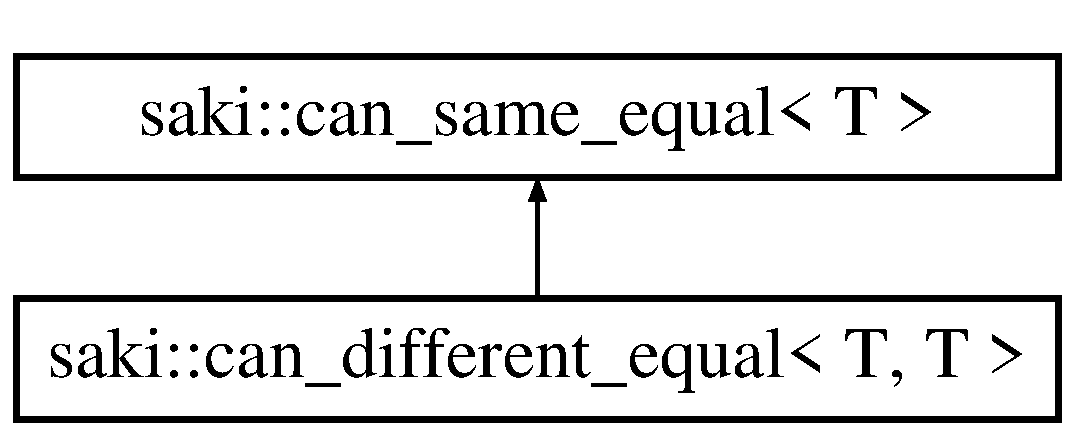
\includegraphics[height=2.000000cm]{structsaki_1_1can__different__equal_3_01_t_00_01_t_01_4}
\end{center}
\end{figure}
\subsection*{その他の継承メンバ}


この構造体詳解は次のファイルから抽出されました\+:\begin{DoxyCompactItemize}
\item 
C\+:/\+Users/tokir/\+Documents/\+Git\+Hub/\+Saki\+Cpp\+Library/saki/type\+\_\+traits/can\+\_\+binary\+\_\+operator/\mbox{\hyperlink{can__equal_8hpp}{can\+\_\+equal.\+hpp}}\end{DoxyCompactItemize}

\hypertarget{structsaki_1_1can__end}{}\section{saki\+:\+:can\+\_\+end$<$ T $>$ 構造体テンプレート}
\label{structsaki_1_1can__end}\index{saki\+::can\+\_\+end$<$ T $>$@{saki\+::can\+\_\+end$<$ T $>$}}


endできるかどうかを判定する構造体  




{\ttfamily \#include $<$can\+\_\+end\+\_\+method.\+hpp$>$}

\subsection*{静的公開変数類}
\begin{DoxyCompactItemize}
\item 
static constexpr auto \mbox{\hyperlink{structsaki_1_1can__end_a5448d219fb1809d8e1bb40ffe2361056}{value}} = decltype(end\+\_\+check$<$T$>$(nullptr))\+::value
\end{DoxyCompactItemize}


\subsection{詳解}
\subsubsection*{template$<$typename T$>$\newline
struct saki\+::can\+\_\+end$<$ T $>$}

endできるかどうかを判定する構造体 

\subsection{メンバ詳解}
\mbox{\Hypertarget{structsaki_1_1can__end_a5448d219fb1809d8e1bb40ffe2361056}\label{structsaki_1_1can__end_a5448d219fb1809d8e1bb40ffe2361056}} 
\index{saki\+::can\+\_\+end@{saki\+::can\+\_\+end}!value@{value}}
\index{value@{value}!saki\+::can\+\_\+end@{saki\+::can\+\_\+end}}
\subsubsection{\texorpdfstring{value}{value}}
{\footnotesize\ttfamily template$<$typename T $>$ \\
constexpr auto \mbox{\hyperlink{structsaki_1_1can__end}{saki\+::can\+\_\+end}}$<$ T $>$\+::value = decltype(end\+\_\+check$<$T$>$(nullptr))\+::value\hspace{0.3cm}{\ttfamily [static]}}



この構造体詳解は次のファイルから抽出されました\+:\begin{DoxyCompactItemize}
\item 
C\+:/\+Users/tokir/\+Documents/\+Git\+Hub/\+Saki\+Cpp\+Library/saki/type\+\_\+traits/\mbox{\hyperlink{can__end__method_8hpp}{can\+\_\+end\+\_\+method.\+hpp}}\end{DoxyCompactItemize}

\hypertarget{structsaki_1_1can__equal__equal}{}\section{saki\+:\+:can\+\_\+equal\+\_\+equal$<$ T $>$ 構造体テンプレート}
\label{structsaki_1_1can__equal__equal}\index{saki\+::can\+\_\+equal\+\_\+equal$<$ T $>$@{saki\+::can\+\_\+equal\+\_\+equal$<$ T $>$}}


イコールイコール比較できるかどうかを判定する構造体(==)  




{\ttfamily \#include $<$can\+\_\+equal\+\_\+equal.\+h$>$}

\subsection*{静的公開変数類}
\begin{DoxyCompactItemize}
\item 
static constexpr auto \mbox{\hyperlink{structsaki_1_1can__equal__equal_a260408f1ad1896949ac2f75caa272211}{value}} = decltype(equal\+\_\+equal\+\_\+check$<$T$>$(nullptr))\+::value
\end{DoxyCompactItemize}


\subsection{詳解}
\subsubsection*{template$<$typename T$>$\newline
struct saki\+::can\+\_\+equal\+\_\+equal$<$ T $>$}

イコールイコール比較できるかどうかを判定する構造体(==) 

\subsection{メンバ詳解}
\mbox{\Hypertarget{structsaki_1_1can__equal__equal_a260408f1ad1896949ac2f75caa272211}\label{structsaki_1_1can__equal__equal_a260408f1ad1896949ac2f75caa272211}} 
\index{saki\+::can\+\_\+equal\+\_\+equal@{saki\+::can\+\_\+equal\+\_\+equal}!value@{value}}
\index{value@{value}!saki\+::can\+\_\+equal\+\_\+equal@{saki\+::can\+\_\+equal\+\_\+equal}}
\subsubsection{\texorpdfstring{value}{value}}
{\footnotesize\ttfamily template$<$typename T $>$ \\
constexpr auto \mbox{\hyperlink{structsaki_1_1can__equal__equal}{saki\+::can\+\_\+equal\+\_\+equal}}$<$ T $>$\+::value = decltype(equal\+\_\+equal\+\_\+check$<$T$>$(nullptr))\+::value\hspace{0.3cm}{\ttfamily [static]}}



この構造体詳解は次のファイルから抽出されました\+:\begin{DoxyCompactItemize}
\item 
C\+:/\+Users/tokir/\+Documents/\+Git\+Hub/\+Saki\+Cpp\+Library/saki/type\+\_\+traits/can\+\_\+compare/\mbox{\hyperlink{can__equal__equal_8h}{can\+\_\+equal\+\_\+equal.\+h}}\end{DoxyCompactItemize}

\hypertarget{structsaki_1_1can__greater}{}\section{saki\+:\+:can\+\_\+greater$<$ T $>$ 構造体テンプレート}
\label{structsaki_1_1can__greater}\index{saki\+::can\+\_\+greater$<$ T $>$@{saki\+::can\+\_\+greater$<$ T $>$}}


より大きい比較できるかどうかを判定する構造体($>$)  




{\ttfamily \#include $<$can\+\_\+greater.\+h$>$}

\subsection*{静的公開変数類}
\begin{DoxyCompactItemize}
\item 
static constexpr auto \mbox{\hyperlink{structsaki_1_1can__greater_a75ef553abd1f49c63f4d31fed7f1f51f}{value}} = decltype(greater\+\_\+check$<$T$>$(nullptr))\+::value
\end{DoxyCompactItemize}


\subsection{詳解}
\subsubsection*{template$<$typename T$>$\newline
struct saki\+::can\+\_\+greater$<$ T $>$}

より大きい比較できるかどうかを判定する構造体($>$) 

\subsection{メンバ詳解}
\mbox{\Hypertarget{structsaki_1_1can__greater_a75ef553abd1f49c63f4d31fed7f1f51f}\label{structsaki_1_1can__greater_a75ef553abd1f49c63f4d31fed7f1f51f}} 
\index{saki\+::can\+\_\+greater@{saki\+::can\+\_\+greater}!value@{value}}
\index{value@{value}!saki\+::can\+\_\+greater@{saki\+::can\+\_\+greater}}
\subsubsection{\texorpdfstring{value}{value}}
{\footnotesize\ttfamily template$<$typename T $>$ \\
constexpr auto \mbox{\hyperlink{structsaki_1_1can__greater}{saki\+::can\+\_\+greater}}$<$ T $>$\+::value = decltype(greater\+\_\+check$<$T$>$(nullptr))\+::value\hspace{0.3cm}{\ttfamily [static]}}



この構造体詳解は次のファイルから抽出されました\+:\begin{DoxyCompactItemize}
\item 
C\+:/\+Users/tokir/\+Documents/\+Git\+Hub/\+Saki\+Cpp\+Library/saki/type\+\_\+traits/can\+\_\+compare/\mbox{\hyperlink{can__greater_8h}{can\+\_\+greater.\+h}}\end{DoxyCompactItemize}

\hypertarget{structsaki_1_1can__greater__or__equal}{}\section{saki\+:\+:can\+\_\+greater\+\_\+or\+\_\+equal$<$ T $>$ 構造体テンプレート}
\label{structsaki_1_1can__greater__or__equal}\index{saki\+::can\+\_\+greater\+\_\+or\+\_\+equal$<$ T $>$@{saki\+::can\+\_\+greater\+\_\+or\+\_\+equal$<$ T $>$}}


以上比較できるかどうかを判定する構造体($>$=)  




{\ttfamily \#include $<$can\+\_\+greater\+\_\+or\+\_\+equal.\+h$>$}

\subsection*{静的公開変数類}
\begin{DoxyCompactItemize}
\item 
static constexpr auto \mbox{\hyperlink{structsaki_1_1can__greater__or__equal_a33bdce8a91412add2b2c1a3f4635fb31}{value}} = decltype(greater\+\_\+or\+\_\+equal\+\_\+check$<$T$>$(nullptr))\+::value
\end{DoxyCompactItemize}


\subsection{詳解}
\subsubsection*{template$<$typename T$>$\newline
struct saki\+::can\+\_\+greater\+\_\+or\+\_\+equal$<$ T $>$}

以上比較できるかどうかを判定する構造体($>$=) 

\subsection{メンバ詳解}
\mbox{\Hypertarget{structsaki_1_1can__greater__or__equal_a33bdce8a91412add2b2c1a3f4635fb31}\label{structsaki_1_1can__greater__or__equal_a33bdce8a91412add2b2c1a3f4635fb31}} 
\index{saki\+::can\+\_\+greater\+\_\+or\+\_\+equal@{saki\+::can\+\_\+greater\+\_\+or\+\_\+equal}!value@{value}}
\index{value@{value}!saki\+::can\+\_\+greater\+\_\+or\+\_\+equal@{saki\+::can\+\_\+greater\+\_\+or\+\_\+equal}}
\subsubsection{\texorpdfstring{value}{value}}
{\footnotesize\ttfamily template$<$typename T $>$ \\
constexpr auto \mbox{\hyperlink{structsaki_1_1can__greater__or__equal}{saki\+::can\+\_\+greater\+\_\+or\+\_\+equal}}$<$ T $>$\+::value = decltype(greater\+\_\+or\+\_\+equal\+\_\+check$<$T$>$(nullptr))\+::value\hspace{0.3cm}{\ttfamily [static]}}



この構造体詳解は次のファイルから抽出されました\+:\begin{DoxyCompactItemize}
\item 
C\+:/\+Users/tokir/\+Documents/\+Git\+Hub/\+Saki\+Cpp\+Library/saki/type\+\_\+traits/can\+\_\+compare/\mbox{\hyperlink{can__greater__or__equal_8h}{can\+\_\+greater\+\_\+or\+\_\+equal.\+h}}\end{DoxyCompactItemize}

\hypertarget{structsaki_1_1can__less}{}\section{saki\+:\+:can\+\_\+less$<$ T $>$ 構造体テンプレート}
\label{structsaki_1_1can__less}\index{saki\+::can\+\_\+less$<$ T $>$@{saki\+::can\+\_\+less$<$ T $>$}}


より小さい比較できるかどうかを判定する構造体($<$)  




{\ttfamily \#include $<$can\+\_\+less.\+hpp$>$}

\subsection*{静的公開変数類}
\begin{DoxyCompactItemize}
\item 
static constexpr auto \mbox{\hyperlink{structsaki_1_1can__less_a49490d61ea0770eaf912571ff7219b29}{value}} = decltype(less\+\_\+check$<$T$>$(nullptr))\+::value
\end{DoxyCompactItemize}


\subsection{詳解}
\subsubsection*{template$<$typename T$>$\newline
struct saki\+::can\+\_\+less$<$ T $>$}

より小さい比較できるかどうかを判定する構造体($<$) 

\subsection{メンバ詳解}
\mbox{\Hypertarget{structsaki_1_1can__less_a49490d61ea0770eaf912571ff7219b29}\label{structsaki_1_1can__less_a49490d61ea0770eaf912571ff7219b29}} 
\index{saki\+::can\+\_\+less@{saki\+::can\+\_\+less}!value@{value}}
\index{value@{value}!saki\+::can\+\_\+less@{saki\+::can\+\_\+less}}
\subsubsection{\texorpdfstring{value}{value}}
{\footnotesize\ttfamily template$<$typename T $>$ \\
constexpr auto \mbox{\hyperlink{structsaki_1_1can__less}{saki\+::can\+\_\+less}}$<$ T $>$\+::value = decltype(less\+\_\+check$<$T$>$(nullptr))\+::value\hspace{0.3cm}{\ttfamily [static]}}



この構造体詳解は次のファイルから抽出されました\+:\begin{DoxyCompactItemize}
\item 
C\+:/\+Users/tokir/\+Documents/\+Git\+Hub/\+Saki\+Cpp\+Library/saki/type\+\_\+traits/can\+\_\+compare/\mbox{\hyperlink{can__less_8hpp}{can\+\_\+less.\+hpp}}\end{DoxyCompactItemize}

\hypertarget{structsaki_1_1can__less__or__equal}{}\section{saki\+:\+:can\+\_\+less\+\_\+or\+\_\+equal$<$ T $>$ 構造体テンプレート}
\label{structsaki_1_1can__less__or__equal}\index{saki\+::can\+\_\+less\+\_\+or\+\_\+equal$<$ T $>$@{saki\+::can\+\_\+less\+\_\+or\+\_\+equal$<$ T $>$}}


以下比較できるかどうかを判定する構造体($<$=)  




{\ttfamily \#include $<$can\+\_\+less\+\_\+or\+\_\+equal.\+hpp$>$}

\subsection*{静的公開変数類}
\begin{DoxyCompactItemize}
\item 
static constexpr auto \mbox{\hyperlink{structsaki_1_1can__less__or__equal_a5a0b1635454596a925eae248a7c7d94d}{value}} = decltype(less\+\_\+or\+\_\+equal\+\_\+check$<$T$>$(nullptr))\+::value
\end{DoxyCompactItemize}


\subsection{詳解}
\subsubsection*{template$<$typename T$>$\newline
struct saki\+::can\+\_\+less\+\_\+or\+\_\+equal$<$ T $>$}

以下比較できるかどうかを判定する構造体($<$=) 

\subsection{メンバ詳解}
\mbox{\Hypertarget{structsaki_1_1can__less__or__equal_a5a0b1635454596a925eae248a7c7d94d}\label{structsaki_1_1can__less__or__equal_a5a0b1635454596a925eae248a7c7d94d}} 
\index{saki\+::can\+\_\+less\+\_\+or\+\_\+equal@{saki\+::can\+\_\+less\+\_\+or\+\_\+equal}!value@{value}}
\index{value@{value}!saki\+::can\+\_\+less\+\_\+or\+\_\+equal@{saki\+::can\+\_\+less\+\_\+or\+\_\+equal}}
\subsubsection{\texorpdfstring{value}{value}}
{\footnotesize\ttfamily template$<$typename T $>$ \\
constexpr auto \mbox{\hyperlink{structsaki_1_1can__less__or__equal}{saki\+::can\+\_\+less\+\_\+or\+\_\+equal}}$<$ T $>$\+::value = decltype(less\+\_\+or\+\_\+equal\+\_\+check$<$T$>$(nullptr))\+::value\hspace{0.3cm}{\ttfamily [static]}}



この構造体詳解は次のファイルから抽出されました\+:\begin{DoxyCompactItemize}
\item 
C\+:/\+Users/tokir/\+Documents/\+Git\+Hub/\+Saki\+Cpp\+Library/saki/type\+\_\+traits/can\+\_\+compare/\mbox{\hyperlink{can__less__or__equal_8hpp}{can\+\_\+less\+\_\+or\+\_\+equal.\+hpp}}\end{DoxyCompactItemize}

\hypertarget{structsaki_1_1can__not__equal}{}\section{saki\+:\+:can\+\_\+not\+\_\+equal$<$ T $>$ 構造体テンプレート}
\label{structsaki_1_1can__not__equal}\index{saki\+::can\+\_\+not\+\_\+equal$<$ T $>$@{saki\+::can\+\_\+not\+\_\+equal$<$ T $>$}}


ノットイコール比較できるかどうかを判定する構造体(!=)  




{\ttfamily \#include $<$can\+\_\+not\+\_\+equal.\+hpp$>$}

\subsection*{静的公開変数類}
\begin{DoxyCompactItemize}
\item 
static constexpr auto \mbox{\hyperlink{structsaki_1_1can__not__equal_a5e6df940e64a430f970175377610d460}{value}} = decltype(not\+\_\+equal\+\_\+check$<$T$>$(nullptr))\+::value
\end{DoxyCompactItemize}


\subsection{詳解}
\subsubsection*{template$<$typename T$>$\newline
struct saki\+::can\+\_\+not\+\_\+equal$<$ T $>$}

ノットイコール比較できるかどうかを判定する構造体(!=) 

\subsection{メンバ詳解}
\mbox{\Hypertarget{structsaki_1_1can__not__equal_a5e6df940e64a430f970175377610d460}\label{structsaki_1_1can__not__equal_a5e6df940e64a430f970175377610d460}} 
\index{saki\+::can\+\_\+not\+\_\+equal@{saki\+::can\+\_\+not\+\_\+equal}!value@{value}}
\index{value@{value}!saki\+::can\+\_\+not\+\_\+equal@{saki\+::can\+\_\+not\+\_\+equal}}
\subsubsection{\texorpdfstring{value}{value}}
{\footnotesize\ttfamily template$<$typename T $>$ \\
constexpr auto \mbox{\hyperlink{structsaki_1_1can__not__equal}{saki\+::can\+\_\+not\+\_\+equal}}$<$ T $>$\+::value = decltype(not\+\_\+equal\+\_\+check$<$T$>$(nullptr))\+::value\hspace{0.3cm}{\ttfamily [static]}}



この構造体詳解は次のファイルから抽出されました\+:\begin{DoxyCompactItemize}
\item 
C\+:/\+Users/tokir/\+Documents/\+Git\+Hub/\+Saki\+Cpp\+Library/saki/type\+\_\+traits/can\+\_\+compare/\mbox{\hyperlink{can__not__equal_8hpp}{can\+\_\+not\+\_\+equal.\+hpp}}\end{DoxyCompactItemize}

\hypertarget{structsaki_1_1can__ostream}{}\section{saki\+:\+:can\+\_\+ostream$<$ T $>$ 構造体テンプレート}
\label{structsaki_1_1can__ostream}\index{saki\+::can\+\_\+ostream$<$ T $>$@{saki\+::can\+\_\+ostream$<$ T $>$}}


ostream演算子をオーバーロードしているかどうか判定する構造体(cout)  




{\ttfamily \#include $<$can\+\_\+ostream.\+h$>$}

\subsection*{静的公開変数類}
\begin{DoxyCompactItemize}
\item 
static constexpr auto \mbox{\hyperlink{structsaki_1_1can__ostream_a949a7959b4856ff60149c82f2b1f56fd}{value}} = decltype(ostream\+\_\+check$<$T$>$(nullptr))\+::value
\end{DoxyCompactItemize}


\subsection{詳解}
\subsubsection*{template$<$typename T$>$\newline
struct saki\+::can\+\_\+ostream$<$ T $>$}

ostream演算子をオーバーロードしているかどうか判定する構造体(cout) 

\subsection{メンバ詳解}
\mbox{\Hypertarget{structsaki_1_1can__ostream_a949a7959b4856ff60149c82f2b1f56fd}\label{structsaki_1_1can__ostream_a949a7959b4856ff60149c82f2b1f56fd}} 
\index{saki\+::can\+\_\+ostream@{saki\+::can\+\_\+ostream}!value@{value}}
\index{value@{value}!saki\+::can\+\_\+ostream@{saki\+::can\+\_\+ostream}}
\subsubsection{\texorpdfstring{value}{value}}
{\footnotesize\ttfamily template$<$typename T $>$ \\
constexpr auto \mbox{\hyperlink{structsaki_1_1can__ostream}{saki\+::can\+\_\+ostream}}$<$ T $>$\+::value = decltype(ostream\+\_\+check$<$T$>$(nullptr))\+::value\hspace{0.3cm}{\ttfamily [static]}}



この構造体詳解は次のファイルから抽出されました\+:\begin{DoxyCompactItemize}
\item 
C\+:/\+Users/tokir/\+Documents/\+Git\+Hub/\+Saki\+Cpp\+Library/saki/type\+\_\+traits/\mbox{\hyperlink{can__ostream_8h}{can\+\_\+ostream.\+h}}\end{DoxyCompactItemize}

\hypertarget{classsaki_1_1can__range__based__for}{}\section{saki\+:\+:can\+\_\+range\+\_\+based\+\_\+for$<$ T $>$ クラステンプレート}
\label{classsaki_1_1can__range__based__for}\index{saki\+::can\+\_\+range\+\_\+based\+\_\+for$<$ T $>$@{saki\+::can\+\_\+range\+\_\+based\+\_\+for$<$ T $>$}}


範囲ベースfor文に利用できる型かどうか判定する  




{\ttfamily \#include $<$can\+\_\+range\+\_\+based\+\_\+for.\+h$>$}

\subsection*{静的公開変数類}
\begin{DoxyCompactItemize}
\item 
static constexpr auto \mbox{\hyperlink{classsaki_1_1can__range__based__for_ad9b48de9333c69be9b613f1ccb6b4f13}{value}} = decltype(check\+\_\+range\+\_\+based\+\_\+for$<$T$>$(nullptr))\+::value
\end{DoxyCompactItemize}


\subsection{詳解}
\subsubsection*{template$<$typename T$>$\newline
class saki\+::can\+\_\+range\+\_\+based\+\_\+for$<$ T $>$}

範囲ベースfor文に利用できる型かどうか判定する 

std\+::beginとstd\+::endを利用できればtrueという判定になる 

\subsection{メンバ詳解}
\mbox{\Hypertarget{classsaki_1_1can__range__based__for_ad9b48de9333c69be9b613f1ccb6b4f13}\label{classsaki_1_1can__range__based__for_ad9b48de9333c69be9b613f1ccb6b4f13}} 
\index{saki\+::can\+\_\+range\+\_\+based\+\_\+for@{saki\+::can\+\_\+range\+\_\+based\+\_\+for}!value@{value}}
\index{value@{value}!saki\+::can\+\_\+range\+\_\+based\+\_\+for@{saki\+::can\+\_\+range\+\_\+based\+\_\+for}}
\subsubsection{\texorpdfstring{value}{value}}
{\footnotesize\ttfamily template$<$typename T $>$ \\
constexpr auto \mbox{\hyperlink{classsaki_1_1can__range__based__for}{saki\+::can\+\_\+range\+\_\+based\+\_\+for}}$<$ T $>$\+::value = decltype(check\+\_\+range\+\_\+based\+\_\+for$<$T$>$(nullptr))\+::value\hspace{0.3cm}{\ttfamily [static]}}



このクラス詳解は次のファイルから抽出されました\+:\begin{DoxyCompactItemize}
\item 
C\+:/\+Users/tokir/\+Documents/\+Git\+Hub/\+Saki\+Cpp\+Library/saki/type\+\_\+traits/\mbox{\hyperlink{can__range__based__for_8h}{can\+\_\+range\+\_\+based\+\_\+for.\+h}}\end{DoxyCompactItemize}

\hypertarget{structsaki_1_1can__same__equal}{}\section{saki\+:\+:can\+\_\+same\+\_\+equal$<$ T $>$ 構造体テンプレート}
\label{structsaki_1_1can__same__equal}\index{saki\+::can\+\_\+same\+\_\+equal$<$ T $>$@{saki\+::can\+\_\+same\+\_\+equal$<$ T $>$}}


代入演算子を定義しているかどうかを判定する構造体(同じ型同士)  




{\ttfamily \#include $<$can\+\_\+equal.\+h$>$}

saki\+:\+:can\+\_\+same\+\_\+equal$<$ T $>$ の継承関係図\begin{figure}[H]
\begin{center}
\leavevmode
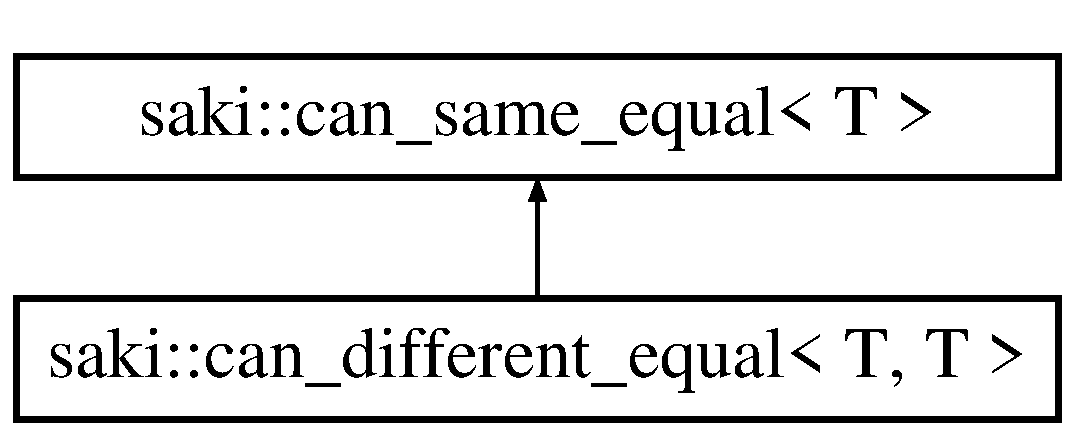
\includegraphics[height=2.000000cm]{structsaki_1_1can__same__equal}
\end{center}
\end{figure}
\subsection*{静的公開変数類}
\begin{DoxyCompactItemize}
\item 
static constexpr auto \mbox{\hyperlink{structsaki_1_1can__same__equal_a7a0e40058e8b1b27113f7fee26fec91f}{value}} = decltype(same\+\_\+equal\+\_\+check$<$T$>$(nullptr))\+::value
\end{DoxyCompactItemize}


\subsection{詳解}
\subsubsection*{template$<$typename T$>$\newline
struct saki\+::can\+\_\+same\+\_\+equal$<$ T $>$}

代入演算子を定義しているかどうかを判定する構造体(同じ型同士) 

\subsection{メンバ詳解}
\mbox{\Hypertarget{structsaki_1_1can__same__equal_a7a0e40058e8b1b27113f7fee26fec91f}\label{structsaki_1_1can__same__equal_a7a0e40058e8b1b27113f7fee26fec91f}} 
\index{saki\+::can\+\_\+same\+\_\+equal@{saki\+::can\+\_\+same\+\_\+equal}!value@{value}}
\index{value@{value}!saki\+::can\+\_\+same\+\_\+equal@{saki\+::can\+\_\+same\+\_\+equal}}
\subsubsection{\texorpdfstring{value}{value}}
{\footnotesize\ttfamily template$<$typename T $>$ \\
constexpr auto \mbox{\hyperlink{structsaki_1_1can__same__equal}{saki\+::can\+\_\+same\+\_\+equal}}$<$ T $>$\+::value = decltype(same\+\_\+equal\+\_\+check$<$T$>$(nullptr))\+::value\hspace{0.3cm}{\ttfamily [static]}}



この構造体詳解は次のファイルから抽出されました\+:\begin{DoxyCompactItemize}
\item 
C\+:/\+Users/tokir/\+Documents/\+Git\+Hub/\+Saki\+Cpp\+Library/saki/type\+\_\+traits/can\+\_\+binary\+\_\+operator/\mbox{\hyperlink{can__equal_8h}{can\+\_\+equal.\+h}}\end{DoxyCompactItemize}

\hypertarget{classsaki_1_1clock}{}\section{saki\+:\+:clock クラス}
\label{classsaki_1_1clock}\index{saki\+::clock@{saki\+::clock}}


時間を測るクラス  




{\ttfamily \#include $<$clock.\+h$>$}

\subsection*{公開型}
\begin{DoxyCompactItemize}
\item 
enum \mbox{\hyperlink{classsaki_1_1clock_a33900ca0b3320bafb061928ad6827bdf}{D\+U\+R\+A\+T\+I\+ON}} \{ \newline
\mbox{\hyperlink{classsaki_1_1clock_a33900ca0b3320bafb061928ad6827bdfadd3f965174e8bb2f64523981626ced1a}{D\+U\+R\+A\+T\+I\+O\+N\+::\+H\+O\+UR}}, 
\mbox{\hyperlink{classsaki_1_1clock_a33900ca0b3320bafb061928ad6827bdfa46bda4cde2f10bdb9e51e3bbefa4a2bf}{D\+U\+R\+A\+T\+I\+O\+N\+::\+M\+I\+N\+U\+TE}}, 
\mbox{\hyperlink{classsaki_1_1clock_a33900ca0b3320bafb061928ad6827bdfa2200becb80f0019c4a2ccecec350d0db}{D\+U\+R\+A\+T\+I\+O\+N\+::\+S\+E\+C\+O\+ND}}, 
\mbox{\hyperlink{classsaki_1_1clock_a33900ca0b3320bafb061928ad6827bdfa241d7907de05ad50c011812e927cd671}{D\+U\+R\+A\+T\+I\+O\+N\+::\+M\+I\+L\+L\+I\+S\+E\+C\+O\+ND}}, 
\newline
\mbox{\hyperlink{classsaki_1_1clock_a33900ca0b3320bafb061928ad6827bdfa52a3ae8e5d772e28d4e2105fefd2eed1}{D\+U\+R\+A\+T\+I\+O\+N\+::\+M\+I\+C\+R\+O\+S\+E\+C\+O\+ND}}, 
\mbox{\hyperlink{classsaki_1_1clock_a33900ca0b3320bafb061928ad6827bdfaeb8c6d69310ffef899148b680e672652}{D\+U\+R\+A\+T\+I\+O\+N\+::\+N\+A\+N\+O\+S\+E\+C\+O\+ND}}, 
\mbox{\hyperlink{classsaki_1_1clock_a33900ca0b3320bafb061928ad6827bdfab50339a10e1de285ac99d4c3990b8693}{D\+U\+R\+A\+T\+I\+O\+N\+::\+N\+O\+NE}}
 \}
\end{DoxyCompactItemize}
\subsection*{公開メンバ関数}
\begin{DoxyCompactItemize}
\item 
\mbox{\hyperlink{classsaki_1_1clock_aec6aa6ad43fcc8f992f7ee9a25e25354}{clock}} ()
\begin{DoxyCompactList}\small\item\em コンストラクタ \end{DoxyCompactList}\item 
void \mbox{\hyperlink{classsaki_1_1clock_ad8c77a4865ba0a3840c640014887a0e3}{start}} ()
\begin{DoxyCompactList}\small\item\em 開始時間のセット \end{DoxyCompactList}\item 
{\footnotesize template$<$typename T  = double, typename saki\+::enable\+\_\+if\+\_\+nullptr\+\_\+t$<$ std\+::is\+\_\+arithmetic\+\_\+v$<$ T $>$$>$  = nullptr$>$ }\\T \mbox{\hyperlink{classsaki_1_1clock_a9d74b8b909a93d819452f175b41d57e4}{end}} (\mbox{\hyperlink{classsaki_1_1clock_a33900ca0b3320bafb061928ad6827bdf}{D\+U\+R\+A\+T\+I\+ON}} duration=\mbox{\hyperlink{classsaki_1_1clock_a33900ca0b3320bafb061928ad6827bdfa241d7907de05ad50c011812e927cd671}{D\+U\+R\+A\+T\+I\+O\+N\+::\+M\+I\+L\+L\+I\+S\+E\+C\+O\+ND}})
\begin{DoxyCompactList}\small\item\em 開始時間をセットしてからの時間を返す \end{DoxyCompactList}\item 
{\footnotesize template$<$typename T  = double, typename saki\+::enable\+\_\+if\+\_\+nullptr\+\_\+t$<$ std\+::is\+\_\+arithmetic\+\_\+v$<$ T $>$$>$  = nullptr$>$ }\\T \mbox{\hyperlink{classsaki_1_1clock_a593da66eb6ce690e20e6602eecfa2b1e}{end\+\_\+and\+\_\+start}} (\mbox{\hyperlink{classsaki_1_1clock_a33900ca0b3320bafb061928ad6827bdf}{D\+U\+R\+A\+T\+I\+ON}} duration=\mbox{\hyperlink{classsaki_1_1clock_a33900ca0b3320bafb061928ad6827bdfa241d7907de05ad50c011812e927cd671}{D\+U\+R\+A\+T\+I\+O\+N\+::\+M\+I\+L\+L\+I\+S\+E\+C\+O\+ND}})
\begin{DoxyCompactList}\small\item\em 開始時間をセットしてからの時間を返し、そこからまた時間をスタートする \end{DoxyCompactList}\end{DoxyCompactItemize}


\subsection{詳解}
時間を測るクラス 

\subsection{列挙型メンバ詳解}
\mbox{\Hypertarget{classsaki_1_1clock_a33900ca0b3320bafb061928ad6827bdf}\label{classsaki_1_1clock_a33900ca0b3320bafb061928ad6827bdf}} 
\index{saki\+::clock@{saki\+::clock}!D\+U\+R\+A\+T\+I\+ON@{D\+U\+R\+A\+T\+I\+ON}}
\index{D\+U\+R\+A\+T\+I\+ON@{D\+U\+R\+A\+T\+I\+ON}!saki\+::clock@{saki\+::clock}}
\subsubsection{\texorpdfstring{D\+U\+R\+A\+T\+I\+ON}{DURATION}}
{\footnotesize\ttfamily enum \mbox{\hyperlink{classsaki_1_1clock_a33900ca0b3320bafb061928ad6827bdf}{saki\+::clock\+::\+D\+U\+R\+A\+T\+I\+ON}}\hspace{0.3cm}{\ttfamily [strong]}}

\begin{DoxyEnumFields}{列挙値}
\raisebox{\heightof{T}}[0pt][0pt]{\index{H\+O\+UR@{H\+O\+UR}!saki\+::clock@{saki\+::clock}}\index{saki\+::clock@{saki\+::clock}!H\+O\+UR@{H\+O\+UR}}}\mbox{\Hypertarget{classsaki_1_1clock_a33900ca0b3320bafb061928ad6827bdfadd3f965174e8bb2f64523981626ced1a}\label{classsaki_1_1clock_a33900ca0b3320bafb061928ad6827bdfadd3f965174e8bb2f64523981626ced1a}} 
H\+O\+UR&\\
\hline

\raisebox{\heightof{T}}[0pt][0pt]{\index{M\+I\+N\+U\+TE@{M\+I\+N\+U\+TE}!saki\+::clock@{saki\+::clock}}\index{saki\+::clock@{saki\+::clock}!M\+I\+N\+U\+TE@{M\+I\+N\+U\+TE}}}\mbox{\Hypertarget{classsaki_1_1clock_a33900ca0b3320bafb061928ad6827bdfa46bda4cde2f10bdb9e51e3bbefa4a2bf}\label{classsaki_1_1clock_a33900ca0b3320bafb061928ad6827bdfa46bda4cde2f10bdb9e51e3bbefa4a2bf}} 
M\+I\+N\+U\+TE&\\
\hline

\raisebox{\heightof{T}}[0pt][0pt]{\index{S\+E\+C\+O\+ND@{S\+E\+C\+O\+ND}!saki\+::clock@{saki\+::clock}}\index{saki\+::clock@{saki\+::clock}!S\+E\+C\+O\+ND@{S\+E\+C\+O\+ND}}}\mbox{\Hypertarget{classsaki_1_1clock_a33900ca0b3320bafb061928ad6827bdfa2200becb80f0019c4a2ccecec350d0db}\label{classsaki_1_1clock_a33900ca0b3320bafb061928ad6827bdfa2200becb80f0019c4a2ccecec350d0db}} 
S\+E\+C\+O\+ND&\\
\hline

\raisebox{\heightof{T}}[0pt][0pt]{\index{M\+I\+L\+L\+I\+S\+E\+C\+O\+ND@{M\+I\+L\+L\+I\+S\+E\+C\+O\+ND}!saki\+::clock@{saki\+::clock}}\index{saki\+::clock@{saki\+::clock}!M\+I\+L\+L\+I\+S\+E\+C\+O\+ND@{M\+I\+L\+L\+I\+S\+E\+C\+O\+ND}}}\mbox{\Hypertarget{classsaki_1_1clock_a33900ca0b3320bafb061928ad6827bdfa241d7907de05ad50c011812e927cd671}\label{classsaki_1_1clock_a33900ca0b3320bafb061928ad6827bdfa241d7907de05ad50c011812e927cd671}} 
M\+I\+L\+L\+I\+S\+E\+C\+O\+ND&\\
\hline

\raisebox{\heightof{T}}[0pt][0pt]{\index{M\+I\+C\+R\+O\+S\+E\+C\+O\+ND@{M\+I\+C\+R\+O\+S\+E\+C\+O\+ND}!saki\+::clock@{saki\+::clock}}\index{saki\+::clock@{saki\+::clock}!M\+I\+C\+R\+O\+S\+E\+C\+O\+ND@{M\+I\+C\+R\+O\+S\+E\+C\+O\+ND}}}\mbox{\Hypertarget{classsaki_1_1clock_a33900ca0b3320bafb061928ad6827bdfa52a3ae8e5d772e28d4e2105fefd2eed1}\label{classsaki_1_1clock_a33900ca0b3320bafb061928ad6827bdfa52a3ae8e5d772e28d4e2105fefd2eed1}} 
M\+I\+C\+R\+O\+S\+E\+C\+O\+ND&\\
\hline

\raisebox{\heightof{T}}[0pt][0pt]{\index{N\+A\+N\+O\+S\+E\+C\+O\+ND@{N\+A\+N\+O\+S\+E\+C\+O\+ND}!saki\+::clock@{saki\+::clock}}\index{saki\+::clock@{saki\+::clock}!N\+A\+N\+O\+S\+E\+C\+O\+ND@{N\+A\+N\+O\+S\+E\+C\+O\+ND}}}\mbox{\Hypertarget{classsaki_1_1clock_a33900ca0b3320bafb061928ad6827bdfaeb8c6d69310ffef899148b680e672652}\label{classsaki_1_1clock_a33900ca0b3320bafb061928ad6827bdfaeb8c6d69310ffef899148b680e672652}} 
N\+A\+N\+O\+S\+E\+C\+O\+ND&\\
\hline

\raisebox{\heightof{T}}[0pt][0pt]{\index{N\+O\+NE@{N\+O\+NE}!saki\+::clock@{saki\+::clock}}\index{saki\+::clock@{saki\+::clock}!N\+O\+NE@{N\+O\+NE}}}\mbox{\Hypertarget{classsaki_1_1clock_a33900ca0b3320bafb061928ad6827bdfab50339a10e1de285ac99d4c3990b8693}\label{classsaki_1_1clock_a33900ca0b3320bafb061928ad6827bdfab50339a10e1de285ac99d4c3990b8693}} 
N\+O\+NE&\\
\hline

\end{DoxyEnumFields}


\subsection{構築子と解体子}
\mbox{\Hypertarget{classsaki_1_1clock_aec6aa6ad43fcc8f992f7ee9a25e25354}\label{classsaki_1_1clock_aec6aa6ad43fcc8f992f7ee9a25e25354}} 
\index{saki\+::clock@{saki\+::clock}!clock@{clock}}
\index{clock@{clock}!saki\+::clock@{saki\+::clock}}
\subsubsection{\texorpdfstring{clock()}{clock()}}
{\footnotesize\ttfamily saki\+::clock\+::clock (\begin{DoxyParamCaption}{ }\end{DoxyParamCaption})\hspace{0.3cm}{\ttfamily [inline]}}



コンストラクタ 



\subsection{関数詳解}
\mbox{\Hypertarget{classsaki_1_1clock_a9d74b8b909a93d819452f175b41d57e4}\label{classsaki_1_1clock_a9d74b8b909a93d819452f175b41d57e4}} 
\index{saki\+::clock@{saki\+::clock}!end@{end}}
\index{end@{end}!saki\+::clock@{saki\+::clock}}
\subsubsection{\texorpdfstring{end()}{end()}}
{\footnotesize\ttfamily template$<$typename T  = double, typename saki\+::enable\+\_\+if\+\_\+nullptr\+\_\+t$<$ std\+::is\+\_\+arithmetic\+\_\+v$<$ T $>$$>$  = nullptr$>$ \\
T saki\+::clock\+::end (\begin{DoxyParamCaption}\item[{\mbox{\hyperlink{classsaki_1_1clock_a33900ca0b3320bafb061928ad6827bdf}{D\+U\+R\+A\+T\+I\+ON}}}]{duration = {\ttfamily \mbox{\hyperlink{classsaki_1_1clock_a33900ca0b3320bafb061928ad6827bdfa241d7907de05ad50c011812e927cd671}{D\+U\+R\+A\+T\+I\+O\+N\+::\+M\+I\+L\+L\+I\+S\+E\+C\+O\+ND}}} }\end{DoxyParamCaption})\hspace{0.3cm}{\ttfamily [inline]}}



開始時間をセットしてからの時間を返す 


\begin{DoxyParams}{引数}
{\em duration} & どの単位で返すか return 時間 \\
\hline
\end{DoxyParams}
\mbox{\Hypertarget{classsaki_1_1clock_a593da66eb6ce690e20e6602eecfa2b1e}\label{classsaki_1_1clock_a593da66eb6ce690e20e6602eecfa2b1e}} 
\index{saki\+::clock@{saki\+::clock}!end\+\_\+and\+\_\+start@{end\+\_\+and\+\_\+start}}
\index{end\+\_\+and\+\_\+start@{end\+\_\+and\+\_\+start}!saki\+::clock@{saki\+::clock}}
\subsubsection{\texorpdfstring{end\+\_\+and\+\_\+start()}{end\_and\_start()}}
{\footnotesize\ttfamily template$<$typename T  = double, typename saki\+::enable\+\_\+if\+\_\+nullptr\+\_\+t$<$ std\+::is\+\_\+arithmetic\+\_\+v$<$ T $>$$>$  = nullptr$>$ \\
T saki\+::clock\+::end\+\_\+and\+\_\+start (\begin{DoxyParamCaption}\item[{\mbox{\hyperlink{classsaki_1_1clock_a33900ca0b3320bafb061928ad6827bdf}{D\+U\+R\+A\+T\+I\+ON}}}]{duration = {\ttfamily \mbox{\hyperlink{classsaki_1_1clock_a33900ca0b3320bafb061928ad6827bdfa241d7907de05ad50c011812e927cd671}{D\+U\+R\+A\+T\+I\+O\+N\+::\+M\+I\+L\+L\+I\+S\+E\+C\+O\+ND}}} }\end{DoxyParamCaption})\hspace{0.3cm}{\ttfamily [inline]}}



開始時間をセットしてからの時間を返し、そこからまた時間をスタートする 


\begin{DoxyParams}{引数}
{\em duration} & どの単位で返すか return 時間 \\
\hline
\end{DoxyParams}
\mbox{\Hypertarget{classsaki_1_1clock_ad8c77a4865ba0a3840c640014887a0e3}\label{classsaki_1_1clock_ad8c77a4865ba0a3840c640014887a0e3}} 
\index{saki\+::clock@{saki\+::clock}!start@{start}}
\index{start@{start}!saki\+::clock@{saki\+::clock}}
\subsubsection{\texorpdfstring{start()}{start()}}
{\footnotesize\ttfamily void saki\+::clock\+::start (\begin{DoxyParamCaption}{ }\end{DoxyParamCaption})\hspace{0.3cm}{\ttfamily [inline]}}



開始時間のセット 



このクラス詳解は次のファイルから抽出されました\+:\begin{DoxyCompactItemize}
\item 
C\+:/\+Users/tokir/\+Documents/\+Git\+Hub/\+Saki\+Cpp\+Library/saki/clock/\mbox{\hyperlink{clock_2clock_8h}{clock.\+h}}\end{DoxyCompactItemize}

\hypertarget{classsaki_1_1const__iterator}{}\section{saki\+:\+:const\+\_\+iterator$<$ T $>$ クラステンプレート}
\label{classsaki_1_1const__iterator}\index{saki\+::const\+\_\+iterator$<$ T $>$@{saki\+::const\+\_\+iterator$<$ T $>$}}


constなイテレーター  




{\ttfamily \#include $<$iterator.\+hpp$>$}

saki\+:\+:const\+\_\+iterator$<$ T $>$ の継承関係図\begin{figure}[H]
\begin{center}
\leavevmode
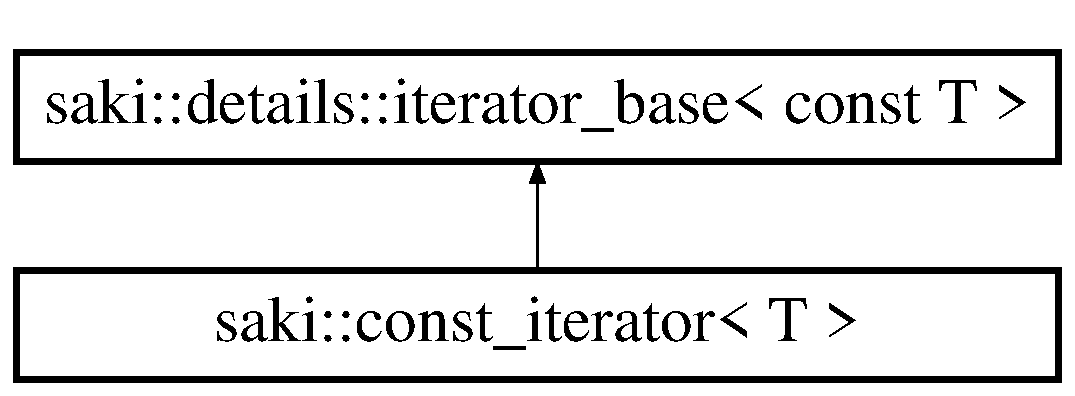
\includegraphics[height=2.000000cm]{classsaki_1_1const__iterator}
\end{center}
\end{figure}
\subsection*{公開メンバ関数}
\begin{DoxyCompactItemize}
\item 
constexpr \mbox{\hyperlink{classsaki_1_1const__iterator_a67dcc4ecf451800f4fa59a536d672ef5}{const\+\_\+iterator}} (const T $\ast$pointer)
\end{DoxyCompactItemize}
\subsection*{その他の継承メンバ}


\subsection{詳解}
\subsubsection*{template$<$typename T$>$\newline
class saki\+::const\+\_\+iterator$<$ T $>$}

constなイテレーター 

\subsection{構築子と解体子}
\mbox{\Hypertarget{classsaki_1_1const__iterator_a67dcc4ecf451800f4fa59a536d672ef5}\label{classsaki_1_1const__iterator_a67dcc4ecf451800f4fa59a536d672ef5}} 
\index{saki\+::const\+\_\+iterator@{saki\+::const\+\_\+iterator}!const\+\_\+iterator@{const\+\_\+iterator}}
\index{const\+\_\+iterator@{const\+\_\+iterator}!saki\+::const\+\_\+iterator@{saki\+::const\+\_\+iterator}}
\subsubsection{\texorpdfstring{const\+\_\+iterator()}{const\_iterator()}}
{\footnotesize\ttfamily template$<$typename T $>$ \\
constexpr \mbox{\hyperlink{classsaki_1_1const__iterator}{saki\+::const\+\_\+iterator}}$<$ T $>$\+::\mbox{\hyperlink{classsaki_1_1const__iterator}{const\+\_\+iterator}} (\begin{DoxyParamCaption}\item[{const T $\ast$}]{pointer }\end{DoxyParamCaption})\hspace{0.3cm}{\ttfamily [inline]}, {\ttfamily [explicit]}}



このクラス詳解は次のファイルから抽出されました\+:\begin{DoxyCompactItemize}
\item 
C\+:/\+Users/tokir/\+Documents/\+Git\+Hub/\+Saki\+Cpp\+Library/saki/iterator/\mbox{\hyperlink{iterator_2iterator_8hpp}{iterator.\+hpp}}\end{DoxyCompactItemize}

\hypertarget{classsaki_1_1const__reverse__iterator}{}\section{saki\+:\+:const\+\_\+reverse\+\_\+iterator$<$ T $>$ クラステンプレート}
\label{classsaki_1_1const__reverse__iterator}\index{saki\+::const\+\_\+reverse\+\_\+iterator$<$ T $>$@{saki\+::const\+\_\+reverse\+\_\+iterator$<$ T $>$}}


constなリバースイテレーター  




{\ttfamily \#include $<$reverse\+\_\+iterator.\+hpp$>$}

saki\+:\+:const\+\_\+reverse\+\_\+iterator$<$ T $>$ の継承関係図\begin{figure}[H]
\begin{center}
\leavevmode
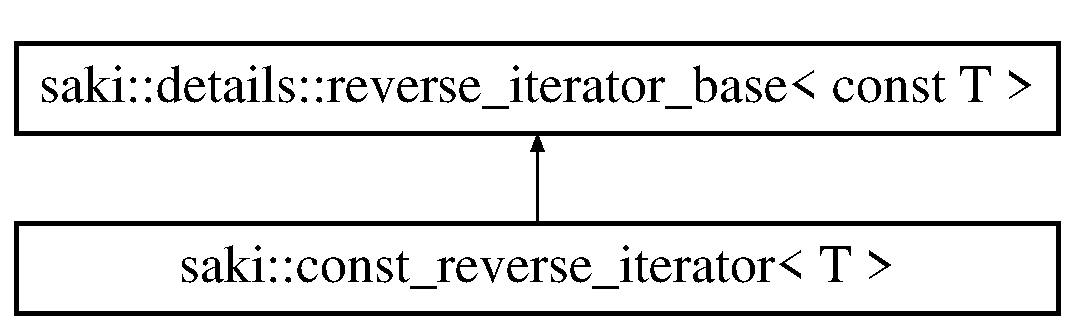
\includegraphics[height=2.000000cm]{classsaki_1_1const__reverse__iterator}
\end{center}
\end{figure}
\subsection*{公開メンバ関数}
\begin{DoxyCompactItemize}
\item 
constexpr \mbox{\hyperlink{classsaki_1_1const__reverse__iterator_ae696e711d884b66fb36c20262446cfae}{const\+\_\+reverse\+\_\+iterator}} (const T pointer)
\end{DoxyCompactItemize}
\subsection*{その他の継承メンバ}


\subsection{詳解}
\subsubsection*{template$<$typename T$>$\newline
class saki\+::const\+\_\+reverse\+\_\+iterator$<$ T $>$}

constなリバースイテレーター 

\subsection{構築子と解体子}
\mbox{\Hypertarget{classsaki_1_1const__reverse__iterator_ae696e711d884b66fb36c20262446cfae}\label{classsaki_1_1const__reverse__iterator_ae696e711d884b66fb36c20262446cfae}} 
\index{saki\+::const\+\_\+reverse\+\_\+iterator@{saki\+::const\+\_\+reverse\+\_\+iterator}!const\+\_\+reverse\+\_\+iterator@{const\+\_\+reverse\+\_\+iterator}}
\index{const\+\_\+reverse\+\_\+iterator@{const\+\_\+reverse\+\_\+iterator}!saki\+::const\+\_\+reverse\+\_\+iterator@{saki\+::const\+\_\+reverse\+\_\+iterator}}
\subsubsection{\texorpdfstring{const\+\_\+reverse\+\_\+iterator()}{const\_reverse\_iterator()}}
{\footnotesize\ttfamily template$<$typename T $>$ \\
constexpr \mbox{\hyperlink{classsaki_1_1const__reverse__iterator}{saki\+::const\+\_\+reverse\+\_\+iterator}}$<$ T $>$\+::\mbox{\hyperlink{classsaki_1_1const__reverse__iterator}{const\+\_\+reverse\+\_\+iterator}} (\begin{DoxyParamCaption}\item[{const T}]{pointer }\end{DoxyParamCaption})\hspace{0.3cm}{\ttfamily [inline]}, {\ttfamily [explicit]}}



このクラス詳解は次のファイルから抽出されました\+:\begin{DoxyCompactItemize}
\item 
C\+:/\+Users/tokir/\+Documents/\+Git\+Hub/\+Saki\+Cpp\+Library/saki/iterator/reverse/\mbox{\hyperlink{reverse__iterator_8hpp}{reverse\+\_\+iterator.\+hpp}}\end{DoxyCompactItemize}

\hypertarget{structsaki_1_1division}{}\section{saki\+:\+:division 構造体}
\label{structsaki_1_1division}\index{saki\+::division@{saki\+::division}}


割り算のconstexpr対応した関数オブジェクト  




{\ttfamily \#include $<$division.\+hpp$>$}

\subsection*{公開メンバ関数}
\begin{DoxyCompactItemize}
\item 
{\footnotesize template$<$typename T1 , typename T2 $>$ }\\constexpr auto \mbox{\hyperlink{structsaki_1_1division_a54652339884419a0b696265b17b32705}{operator()}} (const T1 \&t1, const T2 \&t2) const -\/$>$ decltype(t1/t2)
\end{DoxyCompactItemize}


\subsection{詳解}
割り算のconstexpr対応した関数オブジェクト 

\subsection{関数詳解}
\mbox{\Hypertarget{structsaki_1_1division_a54652339884419a0b696265b17b32705}\label{structsaki_1_1division_a54652339884419a0b696265b17b32705}} 
\index{saki\+::division@{saki\+::division}!operator()@{operator()}}
\index{operator()@{operator()}!saki\+::division@{saki\+::division}}
\subsubsection{\texorpdfstring{operator()()}{operator()()}}
{\footnotesize\ttfamily template$<$typename T1 , typename T2 $>$ \\
constexpr auto saki\+::division\+::operator() (\begin{DoxyParamCaption}\item[{const T1 \&}]{t1,  }\item[{const T2 \&}]{t2 }\end{DoxyParamCaption}) const -\/$>$ decltype(t1 / t2)
	\hspace{0.3cm}{\ttfamily [inline]}}



この構造体詳解は次のファイルから抽出されました\+:\begin{DoxyCompactItemize}
\item 
C\+:/\+Users/tokir/\+Documents/\+Git\+Hub/\+Saki\+Cpp\+Library/saki/function\+\_\+object/\mbox{\hyperlink{division_8hpp}{division.\+hpp}}\end{DoxyCompactItemize}

\hypertarget{structsaki_1_1double__constant}{}\section{saki\+:\+:double\+\_\+constant$<$ Integer, Dec, Zero\+Num $>$ 構造体テンプレート}
\label{structsaki_1_1double__constant}\index{saki\+::double\+\_\+constant$<$ Integer, Dec, Zero\+Num $>$@{saki\+::double\+\_\+constant$<$ Integer, Dec, Zero\+Num $>$}}


倍精度浮動小数点型の定数を表す  




{\ttfamily \#include $<$float\+\_\+constant.\+h$>$}

saki\+:\+:double\+\_\+constant$<$ Integer, Dec, Zero\+Num $>$ の継承関係図\begin{figure}[H]
\begin{center}
\leavevmode
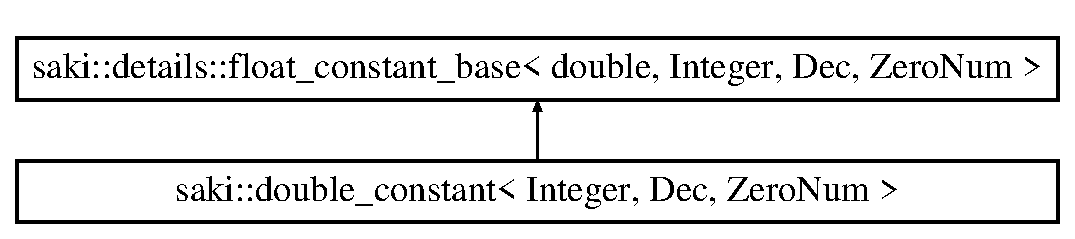
\includegraphics[height=2.000000cm]{structsaki_1_1double__constant}
\end{center}
\end{figure}
\subsection*{その他の継承メンバ}


\subsection{詳解}
\subsubsection*{template$<$int Integer, size\+\_\+t Dec, size\+\_\+t Zero\+Num = 0$>$\newline
struct saki\+::double\+\_\+constant$<$ Integer, Dec, Zero\+Num $>$}

倍精度浮動小数点型の定数を表す 

この構造体詳解は次のファイルから抽出されました\+:\begin{DoxyCompactItemize}
\item 
C\+:/\+Users/tokir/\+Documents/\+Git\+Hub/\+Saki\+Cpp\+Library/saki/type\+\_\+traits/\mbox{\hyperlink{float__constant_8h}{float\+\_\+constant.\+h}}\end{DoxyCompactItemize}

\hypertarget{structsaki_1_1enable__if__nullptr}{}\section{saki\+:\+:enable\+\_\+if\+\_\+nullptr$<$ bool $>$ 構造体テンプレート}
\label{structsaki_1_1enable__if__nullptr}\index{saki\+::enable\+\_\+if\+\_\+nullptr$<$ bool $>$@{saki\+::enable\+\_\+if\+\_\+nullptr$<$ bool $>$}}


enalbe\+\_\+ifのfalse  




{\ttfamily \#include $<$enable\+\_\+if\+\_\+nullptr.\+h$>$}



\subsection{詳解}
\subsubsection*{template$<$bool$>$\newline
struct saki\+::enable\+\_\+if\+\_\+nullptr$<$ bool $>$}

enalbe\+\_\+ifのfalse 

この構造体詳解は次のファイルから抽出されました\+:\begin{DoxyCompactItemize}
\item 
C\+:/\+Users/tokir/\+Documents/\+Git\+Hub/\+Saki\+Cpp\+Library/saki/type\+\_\+traits/\mbox{\hyperlink{enable__if__nullptr_8h}{enable\+\_\+if\+\_\+nullptr.\+h}}\end{DoxyCompactItemize}

\hypertarget{structsaki_1_1enable__if__nullptr_3_01true_01_4}{}\section{saki\+:\+:enable\+\_\+if\+\_\+nullptr$<$ true $>$ 構造体テンプレート}
\label{structsaki_1_1enable__if__nullptr_3_01true_01_4}\index{saki\+::enable\+\_\+if\+\_\+nullptr$<$ true $>$@{saki\+::enable\+\_\+if\+\_\+nullptr$<$ true $>$}}


enable\+\_\+ifのtrue  




{\ttfamily \#include $<$enable\+\_\+if\+\_\+nullptr.\+hpp$>$}

\subsection*{公開型}
\begin{DoxyCompactItemize}
\item 
using \mbox{\hyperlink{structsaki_1_1enable__if__nullptr_3_01true_01_4_a8f1b04372e036f2c7a60c7df41a02e50}{type}} = std\+::nullptr\+\_\+t
\end{DoxyCompactItemize}


\subsection{詳解}
\subsubsection*{template$<$$>$\newline
struct saki\+::enable\+\_\+if\+\_\+nullptr$<$ true $>$}

enable\+\_\+ifのtrue 

\subsection{型定義メンバ詳解}
\mbox{\Hypertarget{structsaki_1_1enable__if__nullptr_3_01true_01_4_a8f1b04372e036f2c7a60c7df41a02e50}\label{structsaki_1_1enable__if__nullptr_3_01true_01_4_a8f1b04372e036f2c7a60c7df41a02e50}} 
\index{saki\+::enable\+\_\+if\+\_\+nullptr$<$ true $>$@{saki\+::enable\+\_\+if\+\_\+nullptr$<$ true $>$}!type@{type}}
\index{type@{type}!saki\+::enable\+\_\+if\+\_\+nullptr$<$ true $>$@{saki\+::enable\+\_\+if\+\_\+nullptr$<$ true $>$}}
\subsubsection{\texorpdfstring{type}{type}}
{\footnotesize\ttfamily using \mbox{\hyperlink{structsaki_1_1enable__if__nullptr}{saki\+::enable\+\_\+if\+\_\+nullptr}}$<$ true $>$\+::\mbox{\hyperlink{structsaki_1_1enable__if__nullptr_3_01true_01_4_a8f1b04372e036f2c7a60c7df41a02e50}{type}} =  std\+::nullptr\+\_\+t}



この構造体詳解は次のファイルから抽出されました\+:\begin{DoxyCompactItemize}
\item 
C\+:/\+Users/tokir/\+Documents/\+Git\+Hub/\+Saki\+Cpp\+Library/saki/type\+\_\+traits/\mbox{\hyperlink{enable__if__nullptr_8hpp}{enable\+\_\+if\+\_\+nullptr.\+hpp}}\end{DoxyCompactItemize}

\hypertarget{structsaki_1_1factorial__limits}{}\section{saki\+:\+:factorial\+\_\+limits$<$ T $>$ 構造体テンプレート}
\label{structsaki_1_1factorial__limits}\index{saki\+::factorial\+\_\+limits$<$ T $>$@{saki\+::factorial\+\_\+limits$<$ T $>$}}


型ごとの最大階乗数  




{\ttfamily \#include $<$factorial.\+h$>$}

\subsection*{静的公開変数類}
\begin{DoxyCompactItemize}
\item 
static constexpr size\+\_\+t \mbox{\hyperlink{structsaki_1_1factorial__limits_af8dce5a6f0fd543e312138b15b92dbe8}{limit}} = 0
\end{DoxyCompactItemize}


\subsection{詳解}
\subsubsection*{template$<$typename T$>$\newline
struct saki\+::factorial\+\_\+limits$<$ T $>$}

型ごとの最大階乗数 

\subsection{メンバ詳解}
\mbox{\Hypertarget{structsaki_1_1factorial__limits_af8dce5a6f0fd543e312138b15b92dbe8}\label{structsaki_1_1factorial__limits_af8dce5a6f0fd543e312138b15b92dbe8}} 
\index{saki\+::factorial\+\_\+limits@{saki\+::factorial\+\_\+limits}!limit@{limit}}
\index{limit@{limit}!saki\+::factorial\+\_\+limits@{saki\+::factorial\+\_\+limits}}
\subsubsection{\texorpdfstring{limit}{limit}}
{\footnotesize\ttfamily template$<$typename T $>$ \\
constexpr size\+\_\+t \mbox{\hyperlink{structsaki_1_1factorial__limits}{saki\+::factorial\+\_\+limits}}$<$ T $>$\+::limit = 0\hspace{0.3cm}{\ttfamily [static]}}



この構造体詳解は次のファイルから抽出されました\+:\begin{DoxyCompactItemize}
\item 
C\+:/\+Users/tokir/\+Documents/\+Git\+Hub/\+Saki\+Cpp\+Library/saki/math/\mbox{\hyperlink{factorial_8h}{factorial.\+h}}\end{DoxyCompactItemize}

\hypertarget{structsaki_1_1factorial__limits_3_01char_01_4}{}\section{saki\+:\+:factorial\+\_\+limits$<$ char $>$ 構造体テンプレート}
\label{structsaki_1_1factorial__limits_3_01char_01_4}\index{saki\+::factorial\+\_\+limits$<$ char $>$@{saki\+::factorial\+\_\+limits$<$ char $>$}}


{\ttfamily \#include $<$factorial.\+h$>$}

\subsection*{静的公開変数類}
\begin{DoxyCompactItemize}
\item 
static constexpr size\+\_\+t \mbox{\hyperlink{structsaki_1_1factorial__limits_3_01char_01_4_a2502b6549e42673f75226ccc6d68a8eb}{limit}} = 5
\end{DoxyCompactItemize}


\subsection{メンバ詳解}
\mbox{\Hypertarget{structsaki_1_1factorial__limits_3_01char_01_4_a2502b6549e42673f75226ccc6d68a8eb}\label{structsaki_1_1factorial__limits_3_01char_01_4_a2502b6549e42673f75226ccc6d68a8eb}} 
\index{saki\+::factorial\+\_\+limits$<$ char $>$@{saki\+::factorial\+\_\+limits$<$ char $>$}!limit@{limit}}
\index{limit@{limit}!saki\+::factorial\+\_\+limits$<$ char $>$@{saki\+::factorial\+\_\+limits$<$ char $>$}}
\subsubsection{\texorpdfstring{limit}{limit}}
{\footnotesize\ttfamily constexpr size\+\_\+t \mbox{\hyperlink{structsaki_1_1factorial__limits}{saki\+::factorial\+\_\+limits}}$<$ char $>$\+::limit = 5\hspace{0.3cm}{\ttfamily [static]}}



この構造体詳解は次のファイルから抽出されました\+:\begin{DoxyCompactItemize}
\item 
C\+:/\+Users/tokir/\+Documents/\+Git\+Hub/\+Saki\+Cpp\+Library/saki/math/\mbox{\hyperlink{factorial_8h}{factorial.\+h}}\end{DoxyCompactItemize}

\hypertarget{structsaki_1_1factorial__limits_3_01char16__t_01_4}{}\section{saki\+:\+:factorial\+\_\+limits$<$ char16\+\_\+t $>$ 構造体テンプレート}
\label{structsaki_1_1factorial__limits_3_01char16__t_01_4}\index{saki\+::factorial\+\_\+limits$<$ char16\+\_\+t $>$@{saki\+::factorial\+\_\+limits$<$ char16\+\_\+t $>$}}


{\ttfamily \#include $<$factorial.\+hpp$>$}

\subsection*{静的公開変数類}
\begin{DoxyCompactItemize}
\item 
static constexpr std\+::size\+\_\+t \mbox{\hyperlink{structsaki_1_1factorial__limits_3_01char16__t_01_4_a8f9b3d37153ef1155b9bc99e5df3a397}{limit}} = 8
\end{DoxyCompactItemize}


\subsection{メンバ詳解}
\mbox{\Hypertarget{structsaki_1_1factorial__limits_3_01char16__t_01_4_a8f9b3d37153ef1155b9bc99e5df3a397}\label{structsaki_1_1factorial__limits_3_01char16__t_01_4_a8f9b3d37153ef1155b9bc99e5df3a397}} 
\index{saki\+::factorial\+\_\+limits$<$ char16\+\_\+t $>$@{saki\+::factorial\+\_\+limits$<$ char16\+\_\+t $>$}!limit@{limit}}
\index{limit@{limit}!saki\+::factorial\+\_\+limits$<$ char16\+\_\+t $>$@{saki\+::factorial\+\_\+limits$<$ char16\+\_\+t $>$}}
\subsubsection{\texorpdfstring{limit}{limit}}
{\footnotesize\ttfamily constexpr std\+::size\+\_\+t \mbox{\hyperlink{structsaki_1_1factorial__limits}{saki\+::factorial\+\_\+limits}}$<$ char16\+\_\+t $>$\+::limit = 8\hspace{0.3cm}{\ttfamily [static]}}



この構造体詳解は次のファイルから抽出されました\+:\begin{DoxyCompactItemize}
\item 
C\+:/\+Users/tokir/\+Documents/\+Git\+Hub/\+Saki\+Cpp\+Library/saki/math/\mbox{\hyperlink{factorial_8hpp}{factorial.\+hpp}}\end{DoxyCompactItemize}

\hypertarget{structsaki_1_1factorial__limits_3_01char32__t_01_4}{}\section{saki\+:\+:factorial\+\_\+limits$<$ char32\+\_\+t $>$ 構造体テンプレート}
\label{structsaki_1_1factorial__limits_3_01char32__t_01_4}\index{saki\+::factorial\+\_\+limits$<$ char32\+\_\+t $>$@{saki\+::factorial\+\_\+limits$<$ char32\+\_\+t $>$}}


{\ttfamily \#include $<$factorial.\+hpp$>$}

\subsection*{静的公開変数類}
\begin{DoxyCompactItemize}
\item 
static constexpr std\+::size\+\_\+t \mbox{\hyperlink{structsaki_1_1factorial__limits_3_01char32__t_01_4_a70ec9b7157ebb1ed3ac25580762ee018}{limit}} = 13
\end{DoxyCompactItemize}


\subsection{メンバ詳解}
\mbox{\Hypertarget{structsaki_1_1factorial__limits_3_01char32__t_01_4_a70ec9b7157ebb1ed3ac25580762ee018}\label{structsaki_1_1factorial__limits_3_01char32__t_01_4_a70ec9b7157ebb1ed3ac25580762ee018}} 
\index{saki\+::factorial\+\_\+limits$<$ char32\+\_\+t $>$@{saki\+::factorial\+\_\+limits$<$ char32\+\_\+t $>$}!limit@{limit}}
\index{limit@{limit}!saki\+::factorial\+\_\+limits$<$ char32\+\_\+t $>$@{saki\+::factorial\+\_\+limits$<$ char32\+\_\+t $>$}}
\subsubsection{\texorpdfstring{limit}{limit}}
{\footnotesize\ttfamily constexpr std\+::size\+\_\+t \mbox{\hyperlink{structsaki_1_1factorial__limits}{saki\+::factorial\+\_\+limits}}$<$ char32\+\_\+t $>$\+::limit = 13\hspace{0.3cm}{\ttfamily [static]}}



この構造体詳解は次のファイルから抽出されました\+:\begin{DoxyCompactItemize}
\item 
C\+:/\+Users/tokir/\+Documents/\+Git\+Hub/\+Saki\+Cpp\+Library/saki/math/\mbox{\hyperlink{factorial_8hpp}{factorial.\+hpp}}\end{DoxyCompactItemize}

\hypertarget{structsaki_1_1factorial__limits_3_01double_01_4}{}\section{saki\+:\+:factorial\+\_\+limits$<$ double $>$ 構造体テンプレート}
\label{structsaki_1_1factorial__limits_3_01double_01_4}\index{saki\+::factorial\+\_\+limits$<$ double $>$@{saki\+::factorial\+\_\+limits$<$ double $>$}}


{\ttfamily \#include $<$factorial.\+hpp$>$}

\subsection*{静的公開変数類}
\begin{DoxyCompactItemize}
\item 
static constexpr std\+::size\+\_\+t \mbox{\hyperlink{structsaki_1_1factorial__limits_3_01double_01_4_aa23876a9fb9d9100d6aa80acf586bfdf}{limit}} = 170
\end{DoxyCompactItemize}


\subsection{メンバ詳解}
\mbox{\Hypertarget{structsaki_1_1factorial__limits_3_01double_01_4_aa23876a9fb9d9100d6aa80acf586bfdf}\label{structsaki_1_1factorial__limits_3_01double_01_4_aa23876a9fb9d9100d6aa80acf586bfdf}} 
\index{saki\+::factorial\+\_\+limits$<$ double $>$@{saki\+::factorial\+\_\+limits$<$ double $>$}!limit@{limit}}
\index{limit@{limit}!saki\+::factorial\+\_\+limits$<$ double $>$@{saki\+::factorial\+\_\+limits$<$ double $>$}}
\subsubsection{\texorpdfstring{limit}{limit}}
{\footnotesize\ttfamily constexpr std\+::size\+\_\+t \mbox{\hyperlink{structsaki_1_1factorial__limits}{saki\+::factorial\+\_\+limits}}$<$ double $>$\+::limit = 170\hspace{0.3cm}{\ttfamily [static]}}



この構造体詳解は次のファイルから抽出されました\+:\begin{DoxyCompactItemize}
\item 
C\+:/\+Users/tokir/\+Documents/\+Git\+Hub/\+Saki\+Cpp\+Library/saki/math/\mbox{\hyperlink{factorial_8hpp}{factorial.\+hpp}}\end{DoxyCompactItemize}

\hypertarget{structsaki_1_1factorial__limits_3_01float_01_4}{}\section{saki\+:\+:factorial\+\_\+limits$<$ float $>$ 構造体テンプレート}
\label{structsaki_1_1factorial__limits_3_01float_01_4}\index{saki\+::factorial\+\_\+limits$<$ float $>$@{saki\+::factorial\+\_\+limits$<$ float $>$}}


{\ttfamily \#include $<$factorial.\+h$>$}

\subsection*{静的公開変数類}
\begin{DoxyCompactItemize}
\item 
static constexpr size\+\_\+t \mbox{\hyperlink{structsaki_1_1factorial__limits_3_01float_01_4_a0ae26b8bc828a91c8e886ce9ba99ad13}{limit}} = 34
\end{DoxyCompactItemize}


\subsection{メンバ詳解}
\mbox{\Hypertarget{structsaki_1_1factorial__limits_3_01float_01_4_a0ae26b8bc828a91c8e886ce9ba99ad13}\label{structsaki_1_1factorial__limits_3_01float_01_4_a0ae26b8bc828a91c8e886ce9ba99ad13}} 
\index{saki\+::factorial\+\_\+limits$<$ float $>$@{saki\+::factorial\+\_\+limits$<$ float $>$}!limit@{limit}}
\index{limit@{limit}!saki\+::factorial\+\_\+limits$<$ float $>$@{saki\+::factorial\+\_\+limits$<$ float $>$}}
\subsubsection{\texorpdfstring{limit}{limit}}
{\footnotesize\ttfamily constexpr size\+\_\+t \mbox{\hyperlink{structsaki_1_1factorial__limits}{saki\+::factorial\+\_\+limits}}$<$ float $>$\+::limit = 34\hspace{0.3cm}{\ttfamily [static]}}



この構造体詳解は次のファイルから抽出されました\+:\begin{DoxyCompactItemize}
\item 
C\+:/\+Users/tokir/\+Documents/\+Git\+Hub/\+Saki\+Cpp\+Library/saki/math/\mbox{\hyperlink{factorial_8h}{factorial.\+h}}\end{DoxyCompactItemize}

\hypertarget{structsaki_1_1factorial__limits_3_01int_01_4}{}\section{saki\+:\+:factorial\+\_\+limits$<$ int $>$ 構造体テンプレート}
\label{structsaki_1_1factorial__limits_3_01int_01_4}\index{saki\+::factorial\+\_\+limits$<$ int $>$@{saki\+::factorial\+\_\+limits$<$ int $>$}}


{\ttfamily \#include $<$factorial.\+h$>$}

\subsection*{静的公開変数類}
\begin{DoxyCompactItemize}
\item 
static constexpr size\+\_\+t \mbox{\hyperlink{structsaki_1_1factorial__limits_3_01int_01_4_a8015f9b9c2d1e4549f2870c70e973b95}{limit}} = 13
\end{DoxyCompactItemize}


\subsection{メンバ詳解}
\mbox{\Hypertarget{structsaki_1_1factorial__limits_3_01int_01_4_a8015f9b9c2d1e4549f2870c70e973b95}\label{structsaki_1_1factorial__limits_3_01int_01_4_a8015f9b9c2d1e4549f2870c70e973b95}} 
\index{saki\+::factorial\+\_\+limits$<$ int $>$@{saki\+::factorial\+\_\+limits$<$ int $>$}!limit@{limit}}
\index{limit@{limit}!saki\+::factorial\+\_\+limits$<$ int $>$@{saki\+::factorial\+\_\+limits$<$ int $>$}}
\subsubsection{\texorpdfstring{limit}{limit}}
{\footnotesize\ttfamily constexpr size\+\_\+t \mbox{\hyperlink{structsaki_1_1factorial__limits}{saki\+::factorial\+\_\+limits}}$<$ int $>$\+::limit = 13\hspace{0.3cm}{\ttfamily [static]}}



この構造体詳解は次のファイルから抽出されました\+:\begin{DoxyCompactItemize}
\item 
C\+:/\+Users/tokir/\+Documents/\+Git\+Hub/\+Saki\+Cpp\+Library/saki/math/\mbox{\hyperlink{factorial_8h}{factorial.\+h}}\end{DoxyCompactItemize}

\hypertarget{structsaki_1_1factorial__limits_3_01long_01_4}{}\section{saki\+:\+:factorial\+\_\+limits$<$ long $>$ 構造体テンプレート}
\label{structsaki_1_1factorial__limits_3_01long_01_4}\index{saki\+::factorial\+\_\+limits$<$ long $>$@{saki\+::factorial\+\_\+limits$<$ long $>$}}


{\ttfamily \#include $<$factorial.\+h$>$}

\subsection*{静的公開変数類}
\begin{DoxyCompactItemize}
\item 
static constexpr size\+\_\+t \mbox{\hyperlink{structsaki_1_1factorial__limits_3_01long_01_4_ae7124e54a372419173270e3142865be2}{limit}} = 13
\end{DoxyCompactItemize}


\subsection{メンバ詳解}
\mbox{\Hypertarget{structsaki_1_1factorial__limits_3_01long_01_4_ae7124e54a372419173270e3142865be2}\label{structsaki_1_1factorial__limits_3_01long_01_4_ae7124e54a372419173270e3142865be2}} 
\index{saki\+::factorial\+\_\+limits$<$ long $>$@{saki\+::factorial\+\_\+limits$<$ long $>$}!limit@{limit}}
\index{limit@{limit}!saki\+::factorial\+\_\+limits$<$ long $>$@{saki\+::factorial\+\_\+limits$<$ long $>$}}
\subsubsection{\texorpdfstring{limit}{limit}}
{\footnotesize\ttfamily constexpr size\+\_\+t \mbox{\hyperlink{structsaki_1_1factorial__limits}{saki\+::factorial\+\_\+limits}}$<$ long $>$\+::limit = 13\hspace{0.3cm}{\ttfamily [static]}}



この構造体詳解は次のファイルから抽出されました\+:\begin{DoxyCompactItemize}
\item 
C\+:/\+Users/tokir/\+Documents/\+Git\+Hub/\+Saki\+Cpp\+Library/saki/math/\mbox{\hyperlink{factorial_8h}{factorial.\+h}}\end{DoxyCompactItemize}

\hypertarget{structsaki_1_1factorial__limits_3_01long_01double_01_4}{}\section{saki\+:\+:factorial\+\_\+limits$<$ long double $>$ 構造体テンプレート}
\label{structsaki_1_1factorial__limits_3_01long_01double_01_4}\index{saki\+::factorial\+\_\+limits$<$ long double $>$@{saki\+::factorial\+\_\+limits$<$ long double $>$}}


{\ttfamily \#include $<$factorial.\+h$>$}

\subsection*{静的公開変数類}
\begin{DoxyCompactItemize}
\item 
static constexpr size\+\_\+t \mbox{\hyperlink{structsaki_1_1factorial__limits_3_01long_01double_01_4_a7b3f995098451f04c6cb8b6626fc9144}{limit}} = 170
\end{DoxyCompactItemize}


\subsection{メンバ詳解}
\mbox{\Hypertarget{structsaki_1_1factorial__limits_3_01long_01double_01_4_a7b3f995098451f04c6cb8b6626fc9144}\label{structsaki_1_1factorial__limits_3_01long_01double_01_4_a7b3f995098451f04c6cb8b6626fc9144}} 
\index{saki\+::factorial\+\_\+limits$<$ long double $>$@{saki\+::factorial\+\_\+limits$<$ long double $>$}!limit@{limit}}
\index{limit@{limit}!saki\+::factorial\+\_\+limits$<$ long double $>$@{saki\+::factorial\+\_\+limits$<$ long double $>$}}
\subsubsection{\texorpdfstring{limit}{limit}}
{\footnotesize\ttfamily constexpr size\+\_\+t \mbox{\hyperlink{structsaki_1_1factorial__limits}{saki\+::factorial\+\_\+limits}}$<$ long double $>$\+::limit = 170\hspace{0.3cm}{\ttfamily [static]}}



この構造体詳解は次のファイルから抽出されました\+:\begin{DoxyCompactItemize}
\item 
C\+:/\+Users/tokir/\+Documents/\+Git\+Hub/\+Saki\+Cpp\+Library/saki/math/\mbox{\hyperlink{factorial_8h}{factorial.\+h}}\end{DoxyCompactItemize}

\hypertarget{structsaki_1_1factorial__limits_3_01long_01long_01_4}{}\section{saki\+:\+:factorial\+\_\+limits$<$ long long $>$ 構造体テンプレート}
\label{structsaki_1_1factorial__limits_3_01long_01long_01_4}\index{saki\+::factorial\+\_\+limits$<$ long long $>$@{saki\+::factorial\+\_\+limits$<$ long long $>$}}


{\ttfamily \#include $<$factorial.\+h$>$}

\subsection*{静的公開変数類}
\begin{DoxyCompactItemize}
\item 
static constexpr size\+\_\+t \mbox{\hyperlink{structsaki_1_1factorial__limits_3_01long_01long_01_4_ae18bb2d394a29c3be5af05cec4454d02}{limit}} = 20
\end{DoxyCompactItemize}


\subsection{メンバ詳解}
\mbox{\Hypertarget{structsaki_1_1factorial__limits_3_01long_01long_01_4_ae18bb2d394a29c3be5af05cec4454d02}\label{structsaki_1_1factorial__limits_3_01long_01long_01_4_ae18bb2d394a29c3be5af05cec4454d02}} 
\index{saki\+::factorial\+\_\+limits$<$ long long $>$@{saki\+::factorial\+\_\+limits$<$ long long $>$}!limit@{limit}}
\index{limit@{limit}!saki\+::factorial\+\_\+limits$<$ long long $>$@{saki\+::factorial\+\_\+limits$<$ long long $>$}}
\subsubsection{\texorpdfstring{limit}{limit}}
{\footnotesize\ttfamily constexpr size\+\_\+t \mbox{\hyperlink{structsaki_1_1factorial__limits}{saki\+::factorial\+\_\+limits}}$<$ long long $>$\+::limit = 20\hspace{0.3cm}{\ttfamily [static]}}



この構造体詳解は次のファイルから抽出されました\+:\begin{DoxyCompactItemize}
\item 
C\+:/\+Users/tokir/\+Documents/\+Git\+Hub/\+Saki\+Cpp\+Library/saki/math/\mbox{\hyperlink{factorial_8h}{factorial.\+h}}\end{DoxyCompactItemize}

\hypertarget{structsaki_1_1factorial__limits_3_01short_01_4}{}\section{saki\+:\+:factorial\+\_\+limits$<$ short $>$ 構造体テンプレート}
\label{structsaki_1_1factorial__limits_3_01short_01_4}\index{saki\+::factorial\+\_\+limits$<$ short $>$@{saki\+::factorial\+\_\+limits$<$ short $>$}}


{\ttfamily \#include $<$factorial.\+hpp$>$}

\subsection*{静的公開変数類}
\begin{DoxyCompactItemize}
\item 
static constexpr std\+::size\+\_\+t \mbox{\hyperlink{structsaki_1_1factorial__limits_3_01short_01_4_ab6e08ed01efb95e0029077725d7133e5}{limit}} = 7
\end{DoxyCompactItemize}


\subsection{メンバ詳解}
\mbox{\Hypertarget{structsaki_1_1factorial__limits_3_01short_01_4_ab6e08ed01efb95e0029077725d7133e5}\label{structsaki_1_1factorial__limits_3_01short_01_4_ab6e08ed01efb95e0029077725d7133e5}} 
\index{saki\+::factorial\+\_\+limits$<$ short $>$@{saki\+::factorial\+\_\+limits$<$ short $>$}!limit@{limit}}
\index{limit@{limit}!saki\+::factorial\+\_\+limits$<$ short $>$@{saki\+::factorial\+\_\+limits$<$ short $>$}}
\subsubsection{\texorpdfstring{limit}{limit}}
{\footnotesize\ttfamily constexpr std\+::size\+\_\+t \mbox{\hyperlink{structsaki_1_1factorial__limits}{saki\+::factorial\+\_\+limits}}$<$ short $>$\+::limit = 7\hspace{0.3cm}{\ttfamily [static]}}



この構造体詳解は次のファイルから抽出されました\+:\begin{DoxyCompactItemize}
\item 
C\+:/\+Users/tokir/\+Documents/\+Git\+Hub/\+Saki\+Cpp\+Library/saki/math/\mbox{\hyperlink{factorial_8hpp}{factorial.\+hpp}}\end{DoxyCompactItemize}

\hypertarget{structsaki_1_1factorial__limits_3_01unsigned_01char_01_4}{}\section{saki\+:\+:factorial\+\_\+limits$<$ unsigned char $>$ 構造体テンプレート}
\label{structsaki_1_1factorial__limits_3_01unsigned_01char_01_4}\index{saki\+::factorial\+\_\+limits$<$ unsigned char $>$@{saki\+::factorial\+\_\+limits$<$ unsigned char $>$}}


{\ttfamily \#include $<$factorial.\+hpp$>$}

\subsection*{静的公開変数類}
\begin{DoxyCompactItemize}
\item 
static constexpr std\+::size\+\_\+t \mbox{\hyperlink{structsaki_1_1factorial__limits_3_01unsigned_01char_01_4_a4062994479e513651e5692ec85439e72}{limit}} = 6
\end{DoxyCompactItemize}


\subsection{メンバ詳解}
\mbox{\Hypertarget{structsaki_1_1factorial__limits_3_01unsigned_01char_01_4_a4062994479e513651e5692ec85439e72}\label{structsaki_1_1factorial__limits_3_01unsigned_01char_01_4_a4062994479e513651e5692ec85439e72}} 
\index{saki\+::factorial\+\_\+limits$<$ unsigned char $>$@{saki\+::factorial\+\_\+limits$<$ unsigned char $>$}!limit@{limit}}
\index{limit@{limit}!saki\+::factorial\+\_\+limits$<$ unsigned char $>$@{saki\+::factorial\+\_\+limits$<$ unsigned char $>$}}
\subsubsection{\texorpdfstring{limit}{limit}}
{\footnotesize\ttfamily constexpr std\+::size\+\_\+t \mbox{\hyperlink{structsaki_1_1factorial__limits}{saki\+::factorial\+\_\+limits}}$<$ unsigned char $>$\+::limit = 6\hspace{0.3cm}{\ttfamily [static]}}



この構造体詳解は次のファイルから抽出されました\+:\begin{DoxyCompactItemize}
\item 
C\+:/\+Users/tokir/\+Documents/\+Git\+Hub/\+Saki\+Cpp\+Library/saki/math/\mbox{\hyperlink{factorial_8hpp}{factorial.\+hpp}}\end{DoxyCompactItemize}

\hypertarget{structsaki_1_1factorial__limits_3_01unsigned_01int_01_4}{}\section{saki\+:\+:factorial\+\_\+limits$<$ unsigned int $>$ 構造体テンプレート}
\label{structsaki_1_1factorial__limits_3_01unsigned_01int_01_4}\index{saki\+::factorial\+\_\+limits$<$ unsigned int $>$@{saki\+::factorial\+\_\+limits$<$ unsigned int $>$}}


{\ttfamily \#include $<$factorial.\+hpp$>$}

\subsection*{静的公開変数類}
\begin{DoxyCompactItemize}
\item 
static constexpr std\+::size\+\_\+t \mbox{\hyperlink{structsaki_1_1factorial__limits_3_01unsigned_01int_01_4_a7dae8b98f0664b63cdf0230cd545ce59}{limit}} = 13
\end{DoxyCompactItemize}


\subsection{メンバ詳解}
\mbox{\Hypertarget{structsaki_1_1factorial__limits_3_01unsigned_01int_01_4_a7dae8b98f0664b63cdf0230cd545ce59}\label{structsaki_1_1factorial__limits_3_01unsigned_01int_01_4_a7dae8b98f0664b63cdf0230cd545ce59}} 
\index{saki\+::factorial\+\_\+limits$<$ unsigned int $>$@{saki\+::factorial\+\_\+limits$<$ unsigned int $>$}!limit@{limit}}
\index{limit@{limit}!saki\+::factorial\+\_\+limits$<$ unsigned int $>$@{saki\+::factorial\+\_\+limits$<$ unsigned int $>$}}
\subsubsection{\texorpdfstring{limit}{limit}}
{\footnotesize\ttfamily constexpr std\+::size\+\_\+t \mbox{\hyperlink{structsaki_1_1factorial__limits}{saki\+::factorial\+\_\+limits}}$<$ unsigned int $>$\+::limit = 13\hspace{0.3cm}{\ttfamily [static]}}



この構造体詳解は次のファイルから抽出されました\+:\begin{DoxyCompactItemize}
\item 
C\+:/\+Users/tokir/\+Documents/\+Git\+Hub/\+Saki\+Cpp\+Library/saki/math/\mbox{\hyperlink{factorial_8hpp}{factorial.\+hpp}}\end{DoxyCompactItemize}

\hypertarget{structsaki_1_1factorial__limits_3_01unsigned_01long_01_4}{}\section{saki\+:\+:factorial\+\_\+limits$<$ unsigned long $>$ 構造体テンプレート}
\label{structsaki_1_1factorial__limits_3_01unsigned_01long_01_4}\index{saki\+::factorial\+\_\+limits$<$ unsigned long $>$@{saki\+::factorial\+\_\+limits$<$ unsigned long $>$}}


{\ttfamily \#include $<$factorial.\+h$>$}

\subsection*{静的公開変数類}
\begin{DoxyCompactItemize}
\item 
static constexpr size\+\_\+t \mbox{\hyperlink{structsaki_1_1factorial__limits_3_01unsigned_01long_01_4_aebc732144c6ce41767d87c7cda6d9abe}{limit}} = 13
\end{DoxyCompactItemize}


\subsection{メンバ詳解}
\mbox{\Hypertarget{structsaki_1_1factorial__limits_3_01unsigned_01long_01_4_aebc732144c6ce41767d87c7cda6d9abe}\label{structsaki_1_1factorial__limits_3_01unsigned_01long_01_4_aebc732144c6ce41767d87c7cda6d9abe}} 
\index{saki\+::factorial\+\_\+limits$<$ unsigned long $>$@{saki\+::factorial\+\_\+limits$<$ unsigned long $>$}!limit@{limit}}
\index{limit@{limit}!saki\+::factorial\+\_\+limits$<$ unsigned long $>$@{saki\+::factorial\+\_\+limits$<$ unsigned long $>$}}
\subsubsection{\texorpdfstring{limit}{limit}}
{\footnotesize\ttfamily constexpr size\+\_\+t \mbox{\hyperlink{structsaki_1_1factorial__limits}{saki\+::factorial\+\_\+limits}}$<$ unsigned long $>$\+::limit = 13\hspace{0.3cm}{\ttfamily [static]}}



この構造体詳解は次のファイルから抽出されました\+:\begin{DoxyCompactItemize}
\item 
C\+:/\+Users/tokir/\+Documents/\+Git\+Hub/\+Saki\+Cpp\+Library/saki/math/\mbox{\hyperlink{factorial_8h}{factorial.\+h}}\end{DoxyCompactItemize}

\hypertarget{structsaki_1_1factorial__limits_3_01unsigned_01long_01long_01_4}{}\section{saki\+:\+:factorial\+\_\+limits$<$ unsigned long long $>$ 構造体テンプレート}
\label{structsaki_1_1factorial__limits_3_01unsigned_01long_01long_01_4}\index{saki\+::factorial\+\_\+limits$<$ unsigned long long $>$@{saki\+::factorial\+\_\+limits$<$ unsigned long long $>$}}


{\ttfamily \#include $<$factorial.\+hpp$>$}

\subsection*{静的公開変数類}
\begin{DoxyCompactItemize}
\item 
static constexpr std\+::size\+\_\+t \mbox{\hyperlink{structsaki_1_1factorial__limits_3_01unsigned_01long_01long_01_4_a14d4262bd332822e739948e6a32394c6}{limit}} = 22
\end{DoxyCompactItemize}


\subsection{メンバ詳解}
\mbox{\Hypertarget{structsaki_1_1factorial__limits_3_01unsigned_01long_01long_01_4_a14d4262bd332822e739948e6a32394c6}\label{structsaki_1_1factorial__limits_3_01unsigned_01long_01long_01_4_a14d4262bd332822e739948e6a32394c6}} 
\index{saki\+::factorial\+\_\+limits$<$ unsigned long long $>$@{saki\+::factorial\+\_\+limits$<$ unsigned long long $>$}!limit@{limit}}
\index{limit@{limit}!saki\+::factorial\+\_\+limits$<$ unsigned long long $>$@{saki\+::factorial\+\_\+limits$<$ unsigned long long $>$}}
\subsubsection{\texorpdfstring{limit}{limit}}
{\footnotesize\ttfamily constexpr std\+::size\+\_\+t \mbox{\hyperlink{structsaki_1_1factorial__limits}{saki\+::factorial\+\_\+limits}}$<$ unsigned long long $>$\+::limit = 22\hspace{0.3cm}{\ttfamily [static]}}



この構造体詳解は次のファイルから抽出されました\+:\begin{DoxyCompactItemize}
\item 
C\+:/\+Users/tokir/\+Documents/\+Git\+Hub/\+Saki\+Cpp\+Library/saki/math/\mbox{\hyperlink{factorial_8hpp}{factorial.\+hpp}}\end{DoxyCompactItemize}

\hypertarget{structsaki_1_1factorial__limits_3_01unsigned_01short_01_4}{}\section{saki\+:\+:factorial\+\_\+limits$<$ unsigned short $>$ 構造体テンプレート}
\label{structsaki_1_1factorial__limits_3_01unsigned_01short_01_4}\index{saki\+::factorial\+\_\+limits$<$ unsigned short $>$@{saki\+::factorial\+\_\+limits$<$ unsigned short $>$}}


{\ttfamily \#include $<$factorial.\+hpp$>$}

\subsection*{静的公開変数類}
\begin{DoxyCompactItemize}
\item 
static constexpr std\+::size\+\_\+t \mbox{\hyperlink{structsaki_1_1factorial__limits_3_01unsigned_01short_01_4_ac406679bfa5d5745f9d7d772c5a9ec83}{limit}} = 8
\end{DoxyCompactItemize}


\subsection{メンバ詳解}
\mbox{\Hypertarget{structsaki_1_1factorial__limits_3_01unsigned_01short_01_4_ac406679bfa5d5745f9d7d772c5a9ec83}\label{structsaki_1_1factorial__limits_3_01unsigned_01short_01_4_ac406679bfa5d5745f9d7d772c5a9ec83}} 
\index{saki\+::factorial\+\_\+limits$<$ unsigned short $>$@{saki\+::factorial\+\_\+limits$<$ unsigned short $>$}!limit@{limit}}
\index{limit@{limit}!saki\+::factorial\+\_\+limits$<$ unsigned short $>$@{saki\+::factorial\+\_\+limits$<$ unsigned short $>$}}
\subsubsection{\texorpdfstring{limit}{limit}}
{\footnotesize\ttfamily constexpr std\+::size\+\_\+t \mbox{\hyperlink{structsaki_1_1factorial__limits}{saki\+::factorial\+\_\+limits}}$<$ unsigned short $>$\+::limit = 8\hspace{0.3cm}{\ttfamily [static]}}



この構造体詳解は次のファイルから抽出されました\+:\begin{DoxyCompactItemize}
\item 
C\+:/\+Users/tokir/\+Documents/\+Git\+Hub/\+Saki\+Cpp\+Library/saki/math/\mbox{\hyperlink{factorial_8hpp}{factorial.\+hpp}}\end{DoxyCompactItemize}

\hypertarget{structsaki_1_1factorial__limits_3_01wchar__t_01_4}{}\section{saki\+:\+:factorial\+\_\+limits$<$ wchar\+\_\+t $>$ 構造体テンプレート}
\label{structsaki_1_1factorial__limits_3_01wchar__t_01_4}\index{saki\+::factorial\+\_\+limits$<$ wchar\+\_\+t $>$@{saki\+::factorial\+\_\+limits$<$ wchar\+\_\+t $>$}}


{\ttfamily \#include $<$factorial.\+h$>$}

\subsection*{静的公開変数類}
\begin{DoxyCompactItemize}
\item 
static constexpr size\+\_\+t \mbox{\hyperlink{structsaki_1_1factorial__limits_3_01wchar__t_01_4_ab3b034cf7691d44b603fa5d4bef8e363}{limit}} = 8
\end{DoxyCompactItemize}


\subsection{メンバ詳解}
\mbox{\Hypertarget{structsaki_1_1factorial__limits_3_01wchar__t_01_4_ab3b034cf7691d44b603fa5d4bef8e363}\label{structsaki_1_1factorial__limits_3_01wchar__t_01_4_ab3b034cf7691d44b603fa5d4bef8e363}} 
\index{saki\+::factorial\+\_\+limits$<$ wchar\+\_\+t $>$@{saki\+::factorial\+\_\+limits$<$ wchar\+\_\+t $>$}!limit@{limit}}
\index{limit@{limit}!saki\+::factorial\+\_\+limits$<$ wchar\+\_\+t $>$@{saki\+::factorial\+\_\+limits$<$ wchar\+\_\+t $>$}}
\subsubsection{\texorpdfstring{limit}{limit}}
{\footnotesize\ttfamily constexpr size\+\_\+t \mbox{\hyperlink{structsaki_1_1factorial__limits}{saki\+::factorial\+\_\+limits}}$<$ wchar\+\_\+t $>$\+::limit = 8\hspace{0.3cm}{\ttfamily [static]}}



この構造体詳解は次のファイルから抽出されました\+:\begin{DoxyCompactItemize}
\item 
C\+:/\+Users/tokir/\+Documents/\+Git\+Hub/\+Saki\+Cpp\+Library/saki/math/\mbox{\hyperlink{factorial_8h}{factorial.\+h}}\end{DoxyCompactItemize}

\hypertarget{structsaki_1_1fibonacci__limits}{}\section{saki\+:\+:fibonacci\+\_\+limits$<$ T $>$ 構造体テンプレート}
\label{structsaki_1_1fibonacci__limits}\index{saki\+::fibonacci\+\_\+limits$<$ T $>$@{saki\+::fibonacci\+\_\+limits$<$ T $>$}}


型ごとのフィボナッチ数  




{\ttfamily \#include $<$fibonacci.\+h$>$}

\subsection*{静的公開変数類}
\begin{DoxyCompactItemize}
\item 
static constexpr size\+\_\+t \mbox{\hyperlink{structsaki_1_1fibonacci__limits_a6dceda8ec10aee5a66f3032e48b2b58d}{limit}} = 0
\end{DoxyCompactItemize}


\subsection{詳解}
\subsubsection*{template$<$typename T$>$\newline
struct saki\+::fibonacci\+\_\+limits$<$ T $>$}

型ごとのフィボナッチ数 

\subsection{メンバ詳解}
\mbox{\Hypertarget{structsaki_1_1fibonacci__limits_a6dceda8ec10aee5a66f3032e48b2b58d}\label{structsaki_1_1fibonacci__limits_a6dceda8ec10aee5a66f3032e48b2b58d}} 
\index{saki\+::fibonacci\+\_\+limits@{saki\+::fibonacci\+\_\+limits}!limit@{limit}}
\index{limit@{limit}!saki\+::fibonacci\+\_\+limits@{saki\+::fibonacci\+\_\+limits}}
\subsubsection{\texorpdfstring{limit}{limit}}
{\footnotesize\ttfamily template$<$typename T $>$ \\
constexpr size\+\_\+t \mbox{\hyperlink{structsaki_1_1fibonacci__limits}{saki\+::fibonacci\+\_\+limits}}$<$ T $>$\+::limit = 0\hspace{0.3cm}{\ttfamily [static]}}



この構造体詳解は次のファイルから抽出されました\+:\begin{DoxyCompactItemize}
\item 
C\+:/\+Users/tokir/\+Documents/\+Git\+Hub/\+Saki\+Cpp\+Library/saki/math/\mbox{\hyperlink{fibonacci_8h}{fibonacci.\+h}}\end{DoxyCompactItemize}

\hypertarget{structsaki_1_1fibonacci__limits_3_01char_01_4}{}\section{saki\+:\+:fibonacci\+\_\+limits$<$ char $>$ 構造体テンプレート}
\label{structsaki_1_1fibonacci__limits_3_01char_01_4}\index{saki\+::fibonacci\+\_\+limits$<$ char $>$@{saki\+::fibonacci\+\_\+limits$<$ char $>$}}


{\ttfamily \#include $<$fibonacci.\+hpp$>$}

\subsection*{静的公開変数類}
\begin{DoxyCompactItemize}
\item 
static constexpr std\+::size\+\_\+t \mbox{\hyperlink{structsaki_1_1fibonacci__limits_3_01char_01_4_a61bce7b1ef85d9bcb5d5dd340f7ccc97}{limit}} = 11
\end{DoxyCompactItemize}


\subsection{メンバ詳解}
\mbox{\Hypertarget{structsaki_1_1fibonacci__limits_3_01char_01_4_a61bce7b1ef85d9bcb5d5dd340f7ccc97}\label{structsaki_1_1fibonacci__limits_3_01char_01_4_a61bce7b1ef85d9bcb5d5dd340f7ccc97}} 
\index{saki\+::fibonacci\+\_\+limits$<$ char $>$@{saki\+::fibonacci\+\_\+limits$<$ char $>$}!limit@{limit}}
\index{limit@{limit}!saki\+::fibonacci\+\_\+limits$<$ char $>$@{saki\+::fibonacci\+\_\+limits$<$ char $>$}}
\subsubsection{\texorpdfstring{limit}{limit}}
{\footnotesize\ttfamily constexpr std\+::size\+\_\+t \mbox{\hyperlink{structsaki_1_1fibonacci__limits}{saki\+::fibonacci\+\_\+limits}}$<$ char $>$\+::limit = 11\hspace{0.3cm}{\ttfamily [static]}}



この構造体詳解は次のファイルから抽出されました\+:\begin{DoxyCompactItemize}
\item 
C\+:/\+Users/tokir/\+Documents/\+Git\+Hub/\+Saki\+Cpp\+Library/saki/math/\mbox{\hyperlink{fibonacci_8hpp}{fibonacci.\+hpp}}\end{DoxyCompactItemize}

\hypertarget{structsaki_1_1fibonacci__limits_3_01char16__t_01_4}{}\section{saki\+:\+:fibonacci\+\_\+limits$<$ char16\+\_\+t $>$ 構造体テンプレート}
\label{structsaki_1_1fibonacci__limits_3_01char16__t_01_4}\index{saki\+::fibonacci\+\_\+limits$<$ char16\+\_\+t $>$@{saki\+::fibonacci\+\_\+limits$<$ char16\+\_\+t $>$}}


{\ttfamily \#include $<$fibonacci.\+h$>$}

\subsection*{静的公開変数類}
\begin{DoxyCompactItemize}
\item 
static constexpr size\+\_\+t \mbox{\hyperlink{structsaki_1_1fibonacci__limits_3_01char16__t_01_4_af352a6bb89e5e4cba18c13a927a3a632}{limit}} = 24
\end{DoxyCompactItemize}


\subsection{メンバ詳解}
\mbox{\Hypertarget{structsaki_1_1fibonacci__limits_3_01char16__t_01_4_af352a6bb89e5e4cba18c13a927a3a632}\label{structsaki_1_1fibonacci__limits_3_01char16__t_01_4_af352a6bb89e5e4cba18c13a927a3a632}} 
\index{saki\+::fibonacci\+\_\+limits$<$ char16\+\_\+t $>$@{saki\+::fibonacci\+\_\+limits$<$ char16\+\_\+t $>$}!limit@{limit}}
\index{limit@{limit}!saki\+::fibonacci\+\_\+limits$<$ char16\+\_\+t $>$@{saki\+::fibonacci\+\_\+limits$<$ char16\+\_\+t $>$}}
\subsubsection{\texorpdfstring{limit}{limit}}
{\footnotesize\ttfamily constexpr size\+\_\+t \mbox{\hyperlink{structsaki_1_1fibonacci__limits}{saki\+::fibonacci\+\_\+limits}}$<$ char16\+\_\+t $>$\+::limit = 24\hspace{0.3cm}{\ttfamily [static]}}



この構造体詳解は次のファイルから抽出されました\+:\begin{DoxyCompactItemize}
\item 
C\+:/\+Users/tokir/\+Documents/\+Git\+Hub/\+Saki\+Cpp\+Library/saki/math/\mbox{\hyperlink{fibonacci_8h}{fibonacci.\+h}}\end{DoxyCompactItemize}

\hypertarget{structsaki_1_1fibonacci__limits_3_01char32__t_01_4}{}\section{saki\+:\+:fibonacci\+\_\+limits$<$ char32\+\_\+t $>$ 構造体テンプレート}
\label{structsaki_1_1fibonacci__limits_3_01char32__t_01_4}\index{saki\+::fibonacci\+\_\+limits$<$ char32\+\_\+t $>$@{saki\+::fibonacci\+\_\+limits$<$ char32\+\_\+t $>$}}


{\ttfamily \#include $<$fibonacci.\+hpp$>$}

\subsection*{静的公開変数類}
\begin{DoxyCompactItemize}
\item 
static constexpr std\+::size\+\_\+t \mbox{\hyperlink{structsaki_1_1fibonacci__limits_3_01char32__t_01_4_acf2b561aca41b7f275abf992c4504c6d}{limit}} = 47
\end{DoxyCompactItemize}


\subsection{メンバ詳解}
\mbox{\Hypertarget{structsaki_1_1fibonacci__limits_3_01char32__t_01_4_acf2b561aca41b7f275abf992c4504c6d}\label{structsaki_1_1fibonacci__limits_3_01char32__t_01_4_acf2b561aca41b7f275abf992c4504c6d}} 
\index{saki\+::fibonacci\+\_\+limits$<$ char32\+\_\+t $>$@{saki\+::fibonacci\+\_\+limits$<$ char32\+\_\+t $>$}!limit@{limit}}
\index{limit@{limit}!saki\+::fibonacci\+\_\+limits$<$ char32\+\_\+t $>$@{saki\+::fibonacci\+\_\+limits$<$ char32\+\_\+t $>$}}
\subsubsection{\texorpdfstring{limit}{limit}}
{\footnotesize\ttfamily constexpr std\+::size\+\_\+t \mbox{\hyperlink{structsaki_1_1fibonacci__limits}{saki\+::fibonacci\+\_\+limits}}$<$ char32\+\_\+t $>$\+::limit = 47\hspace{0.3cm}{\ttfamily [static]}}



この構造体詳解は次のファイルから抽出されました\+:\begin{DoxyCompactItemize}
\item 
C\+:/\+Users/tokir/\+Documents/\+Git\+Hub/\+Saki\+Cpp\+Library/saki/math/\mbox{\hyperlink{fibonacci_8hpp}{fibonacci.\+hpp}}\end{DoxyCompactItemize}

\hypertarget{structsaki_1_1fibonacci__limits_3_01double_01_4}{}\section{saki\+:\+:fibonacci\+\_\+limits$<$ double $>$ 構造体テンプレート}
\label{structsaki_1_1fibonacci__limits_3_01double_01_4}\index{saki\+::fibonacci\+\_\+limits$<$ double $>$@{saki\+::fibonacci\+\_\+limits$<$ double $>$}}


{\ttfamily \#include $<$fibonacci.\+h$>$}

\subsection*{静的公開変数類}
\begin{DoxyCompactItemize}
\item 
static constexpr size\+\_\+t \mbox{\hyperlink{structsaki_1_1fibonacci__limits_3_01double_01_4_a0cb14c0cd3e8fad78c671fc002d0c1b3}{limit}} = 1476
\end{DoxyCompactItemize}


\subsection{メンバ詳解}
\mbox{\Hypertarget{structsaki_1_1fibonacci__limits_3_01double_01_4_a0cb14c0cd3e8fad78c671fc002d0c1b3}\label{structsaki_1_1fibonacci__limits_3_01double_01_4_a0cb14c0cd3e8fad78c671fc002d0c1b3}} 
\index{saki\+::fibonacci\+\_\+limits$<$ double $>$@{saki\+::fibonacci\+\_\+limits$<$ double $>$}!limit@{limit}}
\index{limit@{limit}!saki\+::fibonacci\+\_\+limits$<$ double $>$@{saki\+::fibonacci\+\_\+limits$<$ double $>$}}
\subsubsection{\texorpdfstring{limit}{limit}}
{\footnotesize\ttfamily constexpr size\+\_\+t \mbox{\hyperlink{structsaki_1_1fibonacci__limits}{saki\+::fibonacci\+\_\+limits}}$<$ double $>$\+::limit = 1476\hspace{0.3cm}{\ttfamily [static]}}



この構造体詳解は次のファイルから抽出されました\+:\begin{DoxyCompactItemize}
\item 
C\+:/\+Users/tokir/\+Documents/\+Git\+Hub/\+Saki\+Cpp\+Library/saki/math/\mbox{\hyperlink{fibonacci_8h}{fibonacci.\+h}}\end{DoxyCompactItemize}

\hypertarget{structsaki_1_1fibonacci__limits_3_01float_01_4}{}\section{saki\+:\+:fibonacci\+\_\+limits$<$ float $>$ 構造体テンプレート}
\label{structsaki_1_1fibonacci__limits_3_01float_01_4}\index{saki\+::fibonacci\+\_\+limits$<$ float $>$@{saki\+::fibonacci\+\_\+limits$<$ float $>$}}


{\ttfamily \#include $<$fibonacci.\+h$>$}

\subsection*{静的公開変数類}
\begin{DoxyCompactItemize}
\item 
static constexpr size\+\_\+t \mbox{\hyperlink{structsaki_1_1fibonacci__limits_3_01float_01_4_a973ff4cf0e32a3051888989d25498b76}{limit}} = 186
\end{DoxyCompactItemize}


\subsection{メンバ詳解}
\mbox{\Hypertarget{structsaki_1_1fibonacci__limits_3_01float_01_4_a973ff4cf0e32a3051888989d25498b76}\label{structsaki_1_1fibonacci__limits_3_01float_01_4_a973ff4cf0e32a3051888989d25498b76}} 
\index{saki\+::fibonacci\+\_\+limits$<$ float $>$@{saki\+::fibonacci\+\_\+limits$<$ float $>$}!limit@{limit}}
\index{limit@{limit}!saki\+::fibonacci\+\_\+limits$<$ float $>$@{saki\+::fibonacci\+\_\+limits$<$ float $>$}}
\subsubsection{\texorpdfstring{limit}{limit}}
{\footnotesize\ttfamily constexpr size\+\_\+t \mbox{\hyperlink{structsaki_1_1fibonacci__limits}{saki\+::fibonacci\+\_\+limits}}$<$ float $>$\+::limit = 186\hspace{0.3cm}{\ttfamily [static]}}



この構造体詳解は次のファイルから抽出されました\+:\begin{DoxyCompactItemize}
\item 
C\+:/\+Users/tokir/\+Documents/\+Git\+Hub/\+Saki\+Cpp\+Library/saki/math/\mbox{\hyperlink{fibonacci_8h}{fibonacci.\+h}}\end{DoxyCompactItemize}

\hypertarget{structsaki_1_1fibonacci__limits_3_01int_01_4}{}\section{saki\+:\+:fibonacci\+\_\+limits$<$ int $>$ 構造体テンプレート}
\label{structsaki_1_1fibonacci__limits_3_01int_01_4}\index{saki\+::fibonacci\+\_\+limits$<$ int $>$@{saki\+::fibonacci\+\_\+limits$<$ int $>$}}


{\ttfamily \#include $<$fibonacci.\+h$>$}

\subsection*{静的公開変数類}
\begin{DoxyCompactItemize}
\item 
static constexpr size\+\_\+t \mbox{\hyperlink{structsaki_1_1fibonacci__limits_3_01int_01_4_ae58f6b545454966902baa93e8cef278d}{limit}} = 46
\end{DoxyCompactItemize}


\subsection{メンバ詳解}
\mbox{\Hypertarget{structsaki_1_1fibonacci__limits_3_01int_01_4_ae58f6b545454966902baa93e8cef278d}\label{structsaki_1_1fibonacci__limits_3_01int_01_4_ae58f6b545454966902baa93e8cef278d}} 
\index{saki\+::fibonacci\+\_\+limits$<$ int $>$@{saki\+::fibonacci\+\_\+limits$<$ int $>$}!limit@{limit}}
\index{limit@{limit}!saki\+::fibonacci\+\_\+limits$<$ int $>$@{saki\+::fibonacci\+\_\+limits$<$ int $>$}}
\subsubsection{\texorpdfstring{limit}{limit}}
{\footnotesize\ttfamily constexpr size\+\_\+t \mbox{\hyperlink{structsaki_1_1fibonacci__limits}{saki\+::fibonacci\+\_\+limits}}$<$ int $>$\+::limit = 46\hspace{0.3cm}{\ttfamily [static]}}



この構造体詳解は次のファイルから抽出されました\+:\begin{DoxyCompactItemize}
\item 
C\+:/\+Users/tokir/\+Documents/\+Git\+Hub/\+Saki\+Cpp\+Library/saki/math/\mbox{\hyperlink{fibonacci_8h}{fibonacci.\+h}}\end{DoxyCompactItemize}

\hypertarget{structsaki_1_1fibonacci__limits_3_01long_01_4}{}\section{saki\+:\+:fibonacci\+\_\+limits$<$ long $>$ 構造体テンプレート}
\label{structsaki_1_1fibonacci__limits_3_01long_01_4}\index{saki\+::fibonacci\+\_\+limits$<$ long $>$@{saki\+::fibonacci\+\_\+limits$<$ long $>$}}


{\ttfamily \#include $<$fibonacci.\+hpp$>$}

\subsection*{静的公開変数類}
\begin{DoxyCompactItemize}
\item 
static constexpr std\+::size\+\_\+t \mbox{\hyperlink{structsaki_1_1fibonacci__limits_3_01long_01_4_a134a40f7a46cfc129ae9570fb95f267d}{limit}} = 46
\end{DoxyCompactItemize}


\subsection{メンバ詳解}
\mbox{\Hypertarget{structsaki_1_1fibonacci__limits_3_01long_01_4_a134a40f7a46cfc129ae9570fb95f267d}\label{structsaki_1_1fibonacci__limits_3_01long_01_4_a134a40f7a46cfc129ae9570fb95f267d}} 
\index{saki\+::fibonacci\+\_\+limits$<$ long $>$@{saki\+::fibonacci\+\_\+limits$<$ long $>$}!limit@{limit}}
\index{limit@{limit}!saki\+::fibonacci\+\_\+limits$<$ long $>$@{saki\+::fibonacci\+\_\+limits$<$ long $>$}}
\subsubsection{\texorpdfstring{limit}{limit}}
{\footnotesize\ttfamily constexpr std\+::size\+\_\+t \mbox{\hyperlink{structsaki_1_1fibonacci__limits}{saki\+::fibonacci\+\_\+limits}}$<$ long $>$\+::limit = 46\hspace{0.3cm}{\ttfamily [static]}}



この構造体詳解は次のファイルから抽出されました\+:\begin{DoxyCompactItemize}
\item 
C\+:/\+Users/tokir/\+Documents/\+Git\+Hub/\+Saki\+Cpp\+Library/saki/math/\mbox{\hyperlink{fibonacci_8hpp}{fibonacci.\+hpp}}\end{DoxyCompactItemize}

\hypertarget{structsaki_1_1fibonacci__limits_3_01long_01double_01_4}{}\section{saki\+:\+:fibonacci\+\_\+limits$<$ long double $>$ 構造体テンプレート}
\label{structsaki_1_1fibonacci__limits_3_01long_01double_01_4}\index{saki\+::fibonacci\+\_\+limits$<$ long double $>$@{saki\+::fibonacci\+\_\+limits$<$ long double $>$}}


{\ttfamily \#include $<$fibonacci.\+hpp$>$}

\subsection*{静的公開変数類}
\begin{DoxyCompactItemize}
\item 
static constexpr std\+::size\+\_\+t \mbox{\hyperlink{structsaki_1_1fibonacci__limits_3_01long_01double_01_4_a8e282bac966b4230161c94086f2c0a32}{limit}} = 1476
\end{DoxyCompactItemize}


\subsection{メンバ詳解}
\mbox{\Hypertarget{structsaki_1_1fibonacci__limits_3_01long_01double_01_4_a8e282bac966b4230161c94086f2c0a32}\label{structsaki_1_1fibonacci__limits_3_01long_01double_01_4_a8e282bac966b4230161c94086f2c0a32}} 
\index{saki\+::fibonacci\+\_\+limits$<$ long double $>$@{saki\+::fibonacci\+\_\+limits$<$ long double $>$}!limit@{limit}}
\index{limit@{limit}!saki\+::fibonacci\+\_\+limits$<$ long double $>$@{saki\+::fibonacci\+\_\+limits$<$ long double $>$}}
\subsubsection{\texorpdfstring{limit}{limit}}
{\footnotesize\ttfamily constexpr std\+::size\+\_\+t \mbox{\hyperlink{structsaki_1_1fibonacci__limits}{saki\+::fibonacci\+\_\+limits}}$<$ long double $>$\+::limit = 1476\hspace{0.3cm}{\ttfamily [static]}}



この構造体詳解は次のファイルから抽出されました\+:\begin{DoxyCompactItemize}
\item 
C\+:/\+Users/tokir/\+Documents/\+Git\+Hub/\+Saki\+Cpp\+Library/saki/math/\mbox{\hyperlink{fibonacci_8hpp}{fibonacci.\+hpp}}\end{DoxyCompactItemize}

\hypertarget{structsaki_1_1fibonacci__limits_3_01long_01long_01_4}{}\section{saki\+:\+:fibonacci\+\_\+limits$<$ long long $>$ 構造体テンプレート}
\label{structsaki_1_1fibonacci__limits_3_01long_01long_01_4}\index{saki\+::fibonacci\+\_\+limits$<$ long long $>$@{saki\+::fibonacci\+\_\+limits$<$ long long $>$}}


{\ttfamily \#include $<$fibonacci.\+hpp$>$}

\subsection*{静的公開変数類}
\begin{DoxyCompactItemize}
\item 
static constexpr std\+::size\+\_\+t \mbox{\hyperlink{structsaki_1_1fibonacci__limits_3_01long_01long_01_4_a46c10e09f0e4a8b8d557c9f2fa0cabd1}{limit}} = 92
\end{DoxyCompactItemize}


\subsection{メンバ詳解}
\mbox{\Hypertarget{structsaki_1_1fibonacci__limits_3_01long_01long_01_4_a46c10e09f0e4a8b8d557c9f2fa0cabd1}\label{structsaki_1_1fibonacci__limits_3_01long_01long_01_4_a46c10e09f0e4a8b8d557c9f2fa0cabd1}} 
\index{saki\+::fibonacci\+\_\+limits$<$ long long $>$@{saki\+::fibonacci\+\_\+limits$<$ long long $>$}!limit@{limit}}
\index{limit@{limit}!saki\+::fibonacci\+\_\+limits$<$ long long $>$@{saki\+::fibonacci\+\_\+limits$<$ long long $>$}}
\subsubsection{\texorpdfstring{limit}{limit}}
{\footnotesize\ttfamily constexpr std\+::size\+\_\+t \mbox{\hyperlink{structsaki_1_1fibonacci__limits}{saki\+::fibonacci\+\_\+limits}}$<$ long long $>$\+::limit = 92\hspace{0.3cm}{\ttfamily [static]}}



この構造体詳解は次のファイルから抽出されました\+:\begin{DoxyCompactItemize}
\item 
C\+:/\+Users/tokir/\+Documents/\+Git\+Hub/\+Saki\+Cpp\+Library/saki/math/\mbox{\hyperlink{fibonacci_8hpp}{fibonacci.\+hpp}}\end{DoxyCompactItemize}

\hypertarget{structsaki_1_1fibonacci__limits_3_01short_01_4}{}\section{saki\+:\+:fibonacci\+\_\+limits$<$ short $>$ 構造体テンプレート}
\label{structsaki_1_1fibonacci__limits_3_01short_01_4}\index{saki\+::fibonacci\+\_\+limits$<$ short $>$@{saki\+::fibonacci\+\_\+limits$<$ short $>$}}


{\ttfamily \#include $<$fibonacci.\+h$>$}

\subsection*{静的公開変数類}
\begin{DoxyCompactItemize}
\item 
static constexpr size\+\_\+t \mbox{\hyperlink{structsaki_1_1fibonacci__limits_3_01short_01_4_a610895ef7ef15c8fb9e7c5e431a5dd23}{limit}} = 23
\end{DoxyCompactItemize}


\subsection{メンバ詳解}
\mbox{\Hypertarget{structsaki_1_1fibonacci__limits_3_01short_01_4_a610895ef7ef15c8fb9e7c5e431a5dd23}\label{structsaki_1_1fibonacci__limits_3_01short_01_4_a610895ef7ef15c8fb9e7c5e431a5dd23}} 
\index{saki\+::fibonacci\+\_\+limits$<$ short $>$@{saki\+::fibonacci\+\_\+limits$<$ short $>$}!limit@{limit}}
\index{limit@{limit}!saki\+::fibonacci\+\_\+limits$<$ short $>$@{saki\+::fibonacci\+\_\+limits$<$ short $>$}}
\subsubsection{\texorpdfstring{limit}{limit}}
{\footnotesize\ttfamily constexpr size\+\_\+t \mbox{\hyperlink{structsaki_1_1fibonacci__limits}{saki\+::fibonacci\+\_\+limits}}$<$ short $>$\+::limit = 23\hspace{0.3cm}{\ttfamily [static]}}



この構造体詳解は次のファイルから抽出されました\+:\begin{DoxyCompactItemize}
\item 
C\+:/\+Users/tokir/\+Documents/\+Git\+Hub/\+Saki\+Cpp\+Library/saki/math/\mbox{\hyperlink{fibonacci_8h}{fibonacci.\+h}}\end{DoxyCompactItemize}

\hypertarget{structsaki_1_1fibonacci__limits_3_01unsigned_01char_01_4}{}\section{saki\+:\+:fibonacci\+\_\+limits$<$ unsigned char $>$ 構造体テンプレート}
\label{structsaki_1_1fibonacci__limits_3_01unsigned_01char_01_4}\index{saki\+::fibonacci\+\_\+limits$<$ unsigned char $>$@{saki\+::fibonacci\+\_\+limits$<$ unsigned char $>$}}


{\ttfamily \#include $<$fibonacci.\+hpp$>$}

\subsection*{静的公開変数類}
\begin{DoxyCompactItemize}
\item 
static constexpr std\+::size\+\_\+t \mbox{\hyperlink{structsaki_1_1fibonacci__limits_3_01unsigned_01char_01_4_a00ae7036814f186358f071f632153848}{limit}} = 13
\end{DoxyCompactItemize}


\subsection{メンバ詳解}
\mbox{\Hypertarget{structsaki_1_1fibonacci__limits_3_01unsigned_01char_01_4_a00ae7036814f186358f071f632153848}\label{structsaki_1_1fibonacci__limits_3_01unsigned_01char_01_4_a00ae7036814f186358f071f632153848}} 
\index{saki\+::fibonacci\+\_\+limits$<$ unsigned char $>$@{saki\+::fibonacci\+\_\+limits$<$ unsigned char $>$}!limit@{limit}}
\index{limit@{limit}!saki\+::fibonacci\+\_\+limits$<$ unsigned char $>$@{saki\+::fibonacci\+\_\+limits$<$ unsigned char $>$}}
\subsubsection{\texorpdfstring{limit}{limit}}
{\footnotesize\ttfamily constexpr std\+::size\+\_\+t \mbox{\hyperlink{structsaki_1_1fibonacci__limits}{saki\+::fibonacci\+\_\+limits}}$<$ unsigned char $>$\+::limit = 13\hspace{0.3cm}{\ttfamily [static]}}



この構造体詳解は次のファイルから抽出されました\+:\begin{DoxyCompactItemize}
\item 
C\+:/\+Users/tokir/\+Documents/\+Git\+Hub/\+Saki\+Cpp\+Library/saki/math/\mbox{\hyperlink{fibonacci_8hpp}{fibonacci.\+hpp}}\end{DoxyCompactItemize}

\hypertarget{structsaki_1_1fibonacci__limits_3_01unsigned_01int_01_4}{}\section{saki\+:\+:fibonacci\+\_\+limits$<$ unsigned int $>$ 構造体テンプレート}
\label{structsaki_1_1fibonacci__limits_3_01unsigned_01int_01_4}\index{saki\+::fibonacci\+\_\+limits$<$ unsigned int $>$@{saki\+::fibonacci\+\_\+limits$<$ unsigned int $>$}}


{\ttfamily \#include $<$fibonacci.\+h$>$}

\subsection*{静的公開変数類}
\begin{DoxyCompactItemize}
\item 
static constexpr size\+\_\+t \mbox{\hyperlink{structsaki_1_1fibonacci__limits_3_01unsigned_01int_01_4_ab6a13aa5a6c355d4f80e7315e216ded3}{limit}} = 47
\end{DoxyCompactItemize}


\subsection{メンバ詳解}
\mbox{\Hypertarget{structsaki_1_1fibonacci__limits_3_01unsigned_01int_01_4_ab6a13aa5a6c355d4f80e7315e216ded3}\label{structsaki_1_1fibonacci__limits_3_01unsigned_01int_01_4_ab6a13aa5a6c355d4f80e7315e216ded3}} 
\index{saki\+::fibonacci\+\_\+limits$<$ unsigned int $>$@{saki\+::fibonacci\+\_\+limits$<$ unsigned int $>$}!limit@{limit}}
\index{limit@{limit}!saki\+::fibonacci\+\_\+limits$<$ unsigned int $>$@{saki\+::fibonacci\+\_\+limits$<$ unsigned int $>$}}
\subsubsection{\texorpdfstring{limit}{limit}}
{\footnotesize\ttfamily constexpr size\+\_\+t \mbox{\hyperlink{structsaki_1_1fibonacci__limits}{saki\+::fibonacci\+\_\+limits}}$<$ unsigned int $>$\+::limit = 47\hspace{0.3cm}{\ttfamily [static]}}



この構造体詳解は次のファイルから抽出されました\+:\begin{DoxyCompactItemize}
\item 
C\+:/\+Users/tokir/\+Documents/\+Git\+Hub/\+Saki\+Cpp\+Library/saki/math/\mbox{\hyperlink{fibonacci_8h}{fibonacci.\+h}}\end{DoxyCompactItemize}

\hypertarget{structsaki_1_1fibonacci__limits_3_01unsigned_01long_01_4}{}\section{saki\+:\+:fibonacci\+\_\+limits$<$ unsigned long $>$ 構造体テンプレート}
\label{structsaki_1_1fibonacci__limits_3_01unsigned_01long_01_4}\index{saki\+::fibonacci\+\_\+limits$<$ unsigned long $>$@{saki\+::fibonacci\+\_\+limits$<$ unsigned long $>$}}


{\ttfamily \#include $<$fibonacci.\+hpp$>$}

\subsection*{静的公開変数類}
\begin{DoxyCompactItemize}
\item 
static constexpr std\+::size\+\_\+t \mbox{\hyperlink{structsaki_1_1fibonacci__limits_3_01unsigned_01long_01_4_ad77b6f0ac4e95c53aa88afa682993c98}{limit}} = 47
\end{DoxyCompactItemize}


\subsection{メンバ詳解}
\mbox{\Hypertarget{structsaki_1_1fibonacci__limits_3_01unsigned_01long_01_4_ad77b6f0ac4e95c53aa88afa682993c98}\label{structsaki_1_1fibonacci__limits_3_01unsigned_01long_01_4_ad77b6f0ac4e95c53aa88afa682993c98}} 
\index{saki\+::fibonacci\+\_\+limits$<$ unsigned long $>$@{saki\+::fibonacci\+\_\+limits$<$ unsigned long $>$}!limit@{limit}}
\index{limit@{limit}!saki\+::fibonacci\+\_\+limits$<$ unsigned long $>$@{saki\+::fibonacci\+\_\+limits$<$ unsigned long $>$}}
\subsubsection{\texorpdfstring{limit}{limit}}
{\footnotesize\ttfamily constexpr std\+::size\+\_\+t \mbox{\hyperlink{structsaki_1_1fibonacci__limits}{saki\+::fibonacci\+\_\+limits}}$<$ unsigned long $>$\+::limit = 47\hspace{0.3cm}{\ttfamily [static]}}



この構造体詳解は次のファイルから抽出されました\+:\begin{DoxyCompactItemize}
\item 
C\+:/\+Users/tokir/\+Documents/\+Git\+Hub/\+Saki\+Cpp\+Library/saki/math/\mbox{\hyperlink{fibonacci_8hpp}{fibonacci.\+hpp}}\end{DoxyCompactItemize}

\hypertarget{structsaki_1_1fibonacci__limits_3_01unsigned_01long_01long_01_4}{}\section{saki\+:\+:fibonacci\+\_\+limits$<$ unsigned long long $>$ 構造体テンプレート}
\label{structsaki_1_1fibonacci__limits_3_01unsigned_01long_01long_01_4}\index{saki\+::fibonacci\+\_\+limits$<$ unsigned long long $>$@{saki\+::fibonacci\+\_\+limits$<$ unsigned long long $>$}}


{\ttfamily \#include $<$fibonacci.\+h$>$}

\subsection*{静的公開変数類}
\begin{DoxyCompactItemize}
\item 
static constexpr size\+\_\+t \mbox{\hyperlink{structsaki_1_1fibonacci__limits_3_01unsigned_01long_01long_01_4_a545c9d82d0d2327f0d3e8299953e5492}{limit}} = 93
\end{DoxyCompactItemize}


\subsection{メンバ詳解}
\mbox{\Hypertarget{structsaki_1_1fibonacci__limits_3_01unsigned_01long_01long_01_4_a545c9d82d0d2327f0d3e8299953e5492}\label{structsaki_1_1fibonacci__limits_3_01unsigned_01long_01long_01_4_a545c9d82d0d2327f0d3e8299953e5492}} 
\index{saki\+::fibonacci\+\_\+limits$<$ unsigned long long $>$@{saki\+::fibonacci\+\_\+limits$<$ unsigned long long $>$}!limit@{limit}}
\index{limit@{limit}!saki\+::fibonacci\+\_\+limits$<$ unsigned long long $>$@{saki\+::fibonacci\+\_\+limits$<$ unsigned long long $>$}}
\subsubsection{\texorpdfstring{limit}{limit}}
{\footnotesize\ttfamily constexpr size\+\_\+t \mbox{\hyperlink{structsaki_1_1fibonacci__limits}{saki\+::fibonacci\+\_\+limits}}$<$ unsigned long long $>$\+::limit = 93\hspace{0.3cm}{\ttfamily [static]}}



この構造体詳解は次のファイルから抽出されました\+:\begin{DoxyCompactItemize}
\item 
C\+:/\+Users/tokir/\+Documents/\+Git\+Hub/\+Saki\+Cpp\+Library/saki/math/\mbox{\hyperlink{fibonacci_8h}{fibonacci.\+h}}\end{DoxyCompactItemize}

\hypertarget{structsaki_1_1fibonacci__limits_3_01unsigned_01short_01_4}{}\section{saki\+:\+:fibonacci\+\_\+limits$<$ unsigned short $>$ 構造体テンプレート}
\label{structsaki_1_1fibonacci__limits_3_01unsigned_01short_01_4}\index{saki\+::fibonacci\+\_\+limits$<$ unsigned short $>$@{saki\+::fibonacci\+\_\+limits$<$ unsigned short $>$}}


{\ttfamily \#include $<$fibonacci.\+h$>$}

\subsection*{静的公開変数類}
\begin{DoxyCompactItemize}
\item 
static constexpr size\+\_\+t \mbox{\hyperlink{structsaki_1_1fibonacci__limits_3_01unsigned_01short_01_4_af057ada046d709babcbf257fe1b6b954}{limit}} = 24
\end{DoxyCompactItemize}


\subsection{メンバ詳解}
\mbox{\Hypertarget{structsaki_1_1fibonacci__limits_3_01unsigned_01short_01_4_af057ada046d709babcbf257fe1b6b954}\label{structsaki_1_1fibonacci__limits_3_01unsigned_01short_01_4_af057ada046d709babcbf257fe1b6b954}} 
\index{saki\+::fibonacci\+\_\+limits$<$ unsigned short $>$@{saki\+::fibonacci\+\_\+limits$<$ unsigned short $>$}!limit@{limit}}
\index{limit@{limit}!saki\+::fibonacci\+\_\+limits$<$ unsigned short $>$@{saki\+::fibonacci\+\_\+limits$<$ unsigned short $>$}}
\subsubsection{\texorpdfstring{limit}{limit}}
{\footnotesize\ttfamily constexpr size\+\_\+t \mbox{\hyperlink{structsaki_1_1fibonacci__limits}{saki\+::fibonacci\+\_\+limits}}$<$ unsigned short $>$\+::limit = 24\hspace{0.3cm}{\ttfamily [static]}}



この構造体詳解は次のファイルから抽出されました\+:\begin{DoxyCompactItemize}
\item 
C\+:/\+Users/tokir/\+Documents/\+Git\+Hub/\+Saki\+Cpp\+Library/saki/math/\mbox{\hyperlink{fibonacci_8h}{fibonacci.\+h}}\end{DoxyCompactItemize}

\hypertarget{structsaki_1_1fibonacci__limits_3_01wchar__t_01_4}{}\section{saki\+:\+:fibonacci\+\_\+limits$<$ wchar\+\_\+t $>$ 構造体テンプレート}
\label{structsaki_1_1fibonacci__limits_3_01wchar__t_01_4}\index{saki\+::fibonacci\+\_\+limits$<$ wchar\+\_\+t $>$@{saki\+::fibonacci\+\_\+limits$<$ wchar\+\_\+t $>$}}


{\ttfamily \#include $<$fibonacci.\+hpp$>$}

\subsection*{静的公開変数類}
\begin{DoxyCompactItemize}
\item 
static constexpr std\+::size\+\_\+t \mbox{\hyperlink{structsaki_1_1fibonacci__limits_3_01wchar__t_01_4_a923d2a384d06cda8c9e10939161e909d}{limit}} = 24
\end{DoxyCompactItemize}


\subsection{メンバ詳解}
\mbox{\Hypertarget{structsaki_1_1fibonacci__limits_3_01wchar__t_01_4_a923d2a384d06cda8c9e10939161e909d}\label{structsaki_1_1fibonacci__limits_3_01wchar__t_01_4_a923d2a384d06cda8c9e10939161e909d}} 
\index{saki\+::fibonacci\+\_\+limits$<$ wchar\+\_\+t $>$@{saki\+::fibonacci\+\_\+limits$<$ wchar\+\_\+t $>$}!limit@{limit}}
\index{limit@{limit}!saki\+::fibonacci\+\_\+limits$<$ wchar\+\_\+t $>$@{saki\+::fibonacci\+\_\+limits$<$ wchar\+\_\+t $>$}}
\subsubsection{\texorpdfstring{limit}{limit}}
{\footnotesize\ttfamily constexpr std\+::size\+\_\+t \mbox{\hyperlink{structsaki_1_1fibonacci__limits}{saki\+::fibonacci\+\_\+limits}}$<$ wchar\+\_\+t $>$\+::limit = 24\hspace{0.3cm}{\ttfamily [static]}}



この構造体詳解は次のファイルから抽出されました\+:\begin{DoxyCompactItemize}
\item 
C\+:/\+Users/tokir/\+Documents/\+Git\+Hub/\+Saki\+Cpp\+Library/saki/math/\mbox{\hyperlink{fibonacci_8hpp}{fibonacci.\+hpp}}\end{DoxyCompactItemize}

\hypertarget{structsaki_1_1float__constant}{}\section{saki\+:\+:float\+\_\+constant$<$ Integer, Dec, Zero\+Num $>$ 構造体テンプレート}
\label{structsaki_1_1float__constant}\index{saki\+::float\+\_\+constant$<$ Integer, Dec, Zero\+Num $>$@{saki\+::float\+\_\+constant$<$ Integer, Dec, Zero\+Num $>$}}


浮動小数点型の定数を表す  




{\ttfamily \#include $<$float\+\_\+constant.\+h$>$}

saki\+:\+:float\+\_\+constant$<$ Integer, Dec, Zero\+Num $>$ の継承関係図\begin{figure}[H]
\begin{center}
\leavevmode
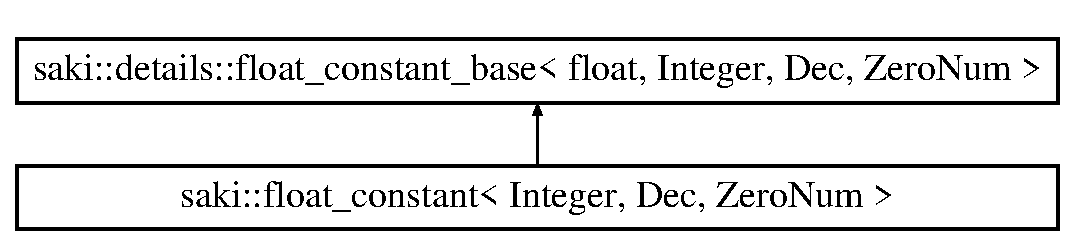
\includegraphics[height=2.000000cm]{structsaki_1_1float__constant}
\end{center}
\end{figure}
\subsection*{その他の継承メンバ}


\subsection{詳解}
\subsubsection*{template$<$int Integer, size\+\_\+t Dec, size\+\_\+t Zero\+Num = 0$>$\newline
struct saki\+::float\+\_\+constant$<$ Integer, Dec, Zero\+Num $>$}

浮動小数点型の定数を表す 

この構造体詳解は次のファイルから抽出されました\+:\begin{DoxyCompactItemize}
\item 
C\+:/\+Users/tokir/\+Documents/\+Git\+Hub/\+Saki\+Cpp\+Library/saki/type\+\_\+traits/\mbox{\hyperlink{float__constant_8h}{float\+\_\+constant.\+h}}\end{DoxyCompactItemize}

\hypertarget{structsaki_1_1details_1_1float__constant__base}{}\section{saki\+:\+:details\+:\+:float\+\_\+constant\+\_\+base$<$ T, Integer, Dec, Zero\+Num $>$ 構造体テンプレート}
\label{structsaki_1_1details_1_1float__constant__base}\index{saki\+::details\+::float\+\_\+constant\+\_\+base$<$ T, Integer, Dec, Zero\+Num $>$@{saki\+::details\+::float\+\_\+constant\+\_\+base$<$ T, Integer, Dec, Zero\+Num $>$}}


浮動小数点型の定数を表すベースクラス  




{\ttfamily \#include $<$float\+\_\+constant.\+hpp$>$}

\subsection*{公開メンバ関数}
\begin{DoxyCompactItemize}
\item 
constexpr \mbox{\hyperlink{structsaki_1_1details_1_1float__constant__base_a35b0e1f79344dc7f1dff6ed2b6209c7d}{operator T}} () const
\item 
constexpr T \mbox{\hyperlink{structsaki_1_1details_1_1float__constant__base_a914139c26ddf5f9664b381a51e6423d4}{operator()}} () const
\end{DoxyCompactItemize}
\subsection*{静的公開変数類}
\begin{DoxyCompactItemize}
\item 
static constexpr T \mbox{\hyperlink{structsaki_1_1details_1_1float__constant__base_a7c1fcb103a7419a7812cf095f1ffff61}{value}}
\end{DoxyCompactItemize}


\subsection{詳解}
\subsubsection*{template$<$typename T, int Integer, size\+\_\+t Dec, size\+\_\+t Zero\+Num = 0$>$\newline
struct saki\+::details\+::float\+\_\+constant\+\_\+base$<$ T, Integer, Dec, Zero\+Num $>$}

浮動小数点型の定数を表すベースクラス 

\subsection{関数詳解}
\mbox{\Hypertarget{structsaki_1_1details_1_1float__constant__base_a35b0e1f79344dc7f1dff6ed2b6209c7d}\label{structsaki_1_1details_1_1float__constant__base_a35b0e1f79344dc7f1dff6ed2b6209c7d}} 
\index{saki\+::details\+::float\+\_\+constant\+\_\+base@{saki\+::details\+::float\+\_\+constant\+\_\+base}!operator T@{operator T}}
\index{operator T@{operator T}!saki\+::details\+::float\+\_\+constant\+\_\+base@{saki\+::details\+::float\+\_\+constant\+\_\+base}}
\subsubsection{\texorpdfstring{operator T()}{operator T()}}
{\footnotesize\ttfamily template$<$typename T, int Integer, size\+\_\+t Dec, size\+\_\+t Zero\+Num = 0$>$ \\
constexpr \mbox{\hyperlink{structsaki_1_1details_1_1float__constant__base}{saki\+::details\+::float\+\_\+constant\+\_\+base}}$<$ T, Integer, Dec, Zero\+Num $>$\+::operator T (\begin{DoxyParamCaption}{ }\end{DoxyParamCaption}) const\hspace{0.3cm}{\ttfamily [inline]}}

\mbox{\Hypertarget{structsaki_1_1details_1_1float__constant__base_a914139c26ddf5f9664b381a51e6423d4}\label{structsaki_1_1details_1_1float__constant__base_a914139c26ddf5f9664b381a51e6423d4}} 
\index{saki\+::details\+::float\+\_\+constant\+\_\+base@{saki\+::details\+::float\+\_\+constant\+\_\+base}!operator()@{operator()}}
\index{operator()@{operator()}!saki\+::details\+::float\+\_\+constant\+\_\+base@{saki\+::details\+::float\+\_\+constant\+\_\+base}}
\subsubsection{\texorpdfstring{operator()()}{operator()()}}
{\footnotesize\ttfamily template$<$typename T, int Integer, size\+\_\+t Dec, size\+\_\+t Zero\+Num = 0$>$ \\
constexpr T \mbox{\hyperlink{structsaki_1_1details_1_1float__constant__base}{saki\+::details\+::float\+\_\+constant\+\_\+base}}$<$ T, Integer, Dec, Zero\+Num $>$\+::operator() (\begin{DoxyParamCaption}{ }\end{DoxyParamCaption}) const\hspace{0.3cm}{\ttfamily [inline]}}



\subsection{メンバ詳解}
\mbox{\Hypertarget{structsaki_1_1details_1_1float__constant__base_a7c1fcb103a7419a7812cf095f1ffff61}\label{structsaki_1_1details_1_1float__constant__base_a7c1fcb103a7419a7812cf095f1ffff61}} 
\index{saki\+::details\+::float\+\_\+constant\+\_\+base@{saki\+::details\+::float\+\_\+constant\+\_\+base}!value@{value}}
\index{value@{value}!saki\+::details\+::float\+\_\+constant\+\_\+base@{saki\+::details\+::float\+\_\+constant\+\_\+base}}
\subsubsection{\texorpdfstring{value}{value}}
{\footnotesize\ttfamily template$<$typename T, int Integer, size\+\_\+t Dec, size\+\_\+t Zero\+Num = 0$>$ \\
constexpr T \mbox{\hyperlink{structsaki_1_1details_1_1float__constant__base}{saki\+::details\+::float\+\_\+constant\+\_\+base}}$<$ T, Integer, Dec, Zero\+Num $>$\+::value\hspace{0.3cm}{\ttfamily [static]}}

{\bfseries 初期値\+:}
\begin{DoxyCode}
= Integer +
                               \mbox{\hyperlink{namespacesaki_a8bab6303ac2144b883080f04ebe26a0e}{saki::copysign}}(static\_cast<T>(Dec) /
                                                  \mbox{\hyperlink{namespacesaki_1_1details_a30b4cd78c970618ee2886123c28e4041}{saki::details::pow\_n}}(static\_cast<T>(1
      0),
                                                                       ZeroNum + 
      \mbox{\hyperlink{namespacesaki_a467dee57b7bbe101146713a82acfe95e}{saki::digit\_count}}(Dec)),
                                              Integer)
\end{DoxyCode}


この構造体詳解は次のファイルから抽出されました\+:\begin{DoxyCompactItemize}
\item 
C\+:/\+Users/tokir/\+Documents/\+Git\+Hub/\+Saki\+Cpp\+Library/saki/type\+\_\+traits/\mbox{\hyperlink{float__constant_8hpp}{float\+\_\+constant.\+hpp}}\end{DoxyCompactItemize}

\hypertarget{structsaki_1_1has__check}{}\section{saki\+:\+:has\+\_\+check$<$ T $>$ 構造体テンプレート}
\label{structsaki_1_1has__check}\index{saki\+::has\+\_\+check$<$ T $>$@{saki\+::has\+\_\+check$<$ T $>$}}


check関数を持っているかどうかを判定する構造体  




{\ttfamily \#include $<$has\+\_\+check\+\_\+method.\+h$>$}

\subsection*{静的公開変数類}
\begin{DoxyCompactItemize}
\item 
static constexpr auto \mbox{\hyperlink{structsaki_1_1has__check_aaf5325bde7c74e8afe2a69f8d657d62b}{value}} = decltype(check\+\_\+check$<$T$>$(nullptr))\+::value
\end{DoxyCompactItemize}


\subsection{詳解}
\subsubsection*{template$<$typename T$>$\newline
struct saki\+::has\+\_\+check$<$ T $>$}

check関数を持っているかどうかを判定する構造体 

\subsection{メンバ詳解}
\mbox{\Hypertarget{structsaki_1_1has__check_aaf5325bde7c74e8afe2a69f8d657d62b}\label{structsaki_1_1has__check_aaf5325bde7c74e8afe2a69f8d657d62b}} 
\index{saki\+::has\+\_\+check@{saki\+::has\+\_\+check}!value@{value}}
\index{value@{value}!saki\+::has\+\_\+check@{saki\+::has\+\_\+check}}
\subsubsection{\texorpdfstring{value}{value}}
{\footnotesize\ttfamily template$<$typename T $>$ \\
constexpr auto \mbox{\hyperlink{structsaki_1_1has__check}{saki\+::has\+\_\+check}}$<$ T $>$\+::value = decltype(check\+\_\+check$<$T$>$(nullptr))\+::value\hspace{0.3cm}{\ttfamily [static]}}



この構造体詳解は次のファイルから抽出されました\+:\begin{DoxyCompactItemize}
\item 
C\+:/\+Users/tokir/\+Documents/\+Git\+Hub/\+Saki\+Cpp\+Library/saki/meta/\mbox{\hyperlink{has__check__method_8h}{has\+\_\+check\+\_\+method.\+h}}\end{DoxyCompactItemize}

\hypertarget{structsaki_1_1has__x}{}\section{saki\+:\+:has\+\_\+x$<$ T $>$ 構造体テンプレート}
\label{structsaki_1_1has__x}\index{saki\+::has\+\_\+x$<$ T $>$@{saki\+::has\+\_\+x$<$ T $>$}}


変数xを持っているかどうかを判定する構造体  




{\ttfamily \#include $<$has\+\_\+variable.\+h$>$}

\subsection*{静的公開変数類}
\begin{DoxyCompactItemize}
\item 
static constexpr auto \mbox{\hyperlink{structsaki_1_1has__x_aa3b89fa1981c7d31e7ec0c70ea01b451}{value}} = decltype(check\+\_\+check$<$T$>$(nullptr))\+::value
\end{DoxyCompactItemize}


\subsection{詳解}
\subsubsection*{template$<$typename T$>$\newline
struct saki\+::has\+\_\+x$<$ T $>$}

変数xを持っているかどうかを判定する構造体 

\subsection{メンバ詳解}
\mbox{\Hypertarget{structsaki_1_1has__x_aa3b89fa1981c7d31e7ec0c70ea01b451}\label{structsaki_1_1has__x_aa3b89fa1981c7d31e7ec0c70ea01b451}} 
\index{saki\+::has\+\_\+x@{saki\+::has\+\_\+x}!value@{value}}
\index{value@{value}!saki\+::has\+\_\+x@{saki\+::has\+\_\+x}}
\subsubsection{\texorpdfstring{value}{value}}
{\footnotesize\ttfamily template$<$typename T $>$ \\
constexpr auto \mbox{\hyperlink{structsaki_1_1has__x}{saki\+::has\+\_\+x}}$<$ T $>$\+::value = decltype(check\+\_\+check$<$T$>$(nullptr))\+::value\hspace{0.3cm}{\ttfamily [static]}}



この構造体詳解は次のファイルから抽出されました\+:\begin{DoxyCompactItemize}
\item 
C\+:/\+Users/tokir/\+Documents/\+Git\+Hub/\+Saki\+Cpp\+Library/saki/type\+\_\+traits/\mbox{\hyperlink{has__variable_8h}{has\+\_\+variable.\+h}}\end{DoxyCompactItemize}

\hypertarget{structsaki_1_1has__y}{}\section{saki\+:\+:has\+\_\+y$<$ T $>$ 構造体テンプレート}
\label{structsaki_1_1has__y}\index{saki\+::has\+\_\+y$<$ T $>$@{saki\+::has\+\_\+y$<$ T $>$}}


変数yを持っているかどうかを判定する構造体  




{\ttfamily \#include $<$has\+\_\+y.\+hpp$>$}

\subsection*{静的公開変数類}
\begin{DoxyCompactItemize}
\item 
static constexpr auto \mbox{\hyperlink{structsaki_1_1has__y_aa7f43916663394a6d3b07295be5cc1ee}{value}} = decltype(y\+\_\+check$<$T$>$(nullptr))\+::value
\end{DoxyCompactItemize}


\subsection{詳解}
\subsubsection*{template$<$typename T$>$\newline
struct saki\+::has\+\_\+y$<$ T $>$}

変数yを持っているかどうかを判定する構造体 

\subsection{メンバ詳解}
\mbox{\Hypertarget{structsaki_1_1has__y_aa7f43916663394a6d3b07295be5cc1ee}\label{structsaki_1_1has__y_aa7f43916663394a6d3b07295be5cc1ee}} 
\index{saki\+::has\+\_\+y@{saki\+::has\+\_\+y}!value@{value}}
\index{value@{value}!saki\+::has\+\_\+y@{saki\+::has\+\_\+y}}
\subsubsection{\texorpdfstring{value}{value}}
{\footnotesize\ttfamily template$<$typename T $>$ \\
constexpr auto \mbox{\hyperlink{structsaki_1_1has__y}{saki\+::has\+\_\+y}}$<$ T $>$\+::value = decltype(y\+\_\+check$<$T$>$(nullptr))\+::value\hspace{0.3cm}{\ttfamily [static]}}



この構造体詳解は次のファイルから抽出されました\+:\begin{DoxyCompactItemize}
\item 
C\+:/\+Users/tokir/\+Documents/\+Git\+Hub/\+Saki\+Cpp\+Library/saki/type\+\_\+traits/has\+\_\+variable/\mbox{\hyperlink{has__y_8hpp}{has\+\_\+y.\+hpp}}\end{DoxyCompactItemize}

\hypertarget{structsaki_1_1has__z}{}\section{saki\+:\+:has\+\_\+z$<$ T $>$ 構造体テンプレート}
\label{structsaki_1_1has__z}\index{saki\+::has\+\_\+z$<$ T $>$@{saki\+::has\+\_\+z$<$ T $>$}}


変数yを持っているかどうかを判定する構造体  




{\ttfamily \#include $<$has\+\_\+z.\+h$>$}

\subsection*{静的公開変数類}
\begin{DoxyCompactItemize}
\item 
static constexpr auto \mbox{\hyperlink{structsaki_1_1has__z_a4abee363bc8a82bb0030300abba45ceb}{value}} = decltype(z\+\_\+check$<$T$>$(nullptr))\+::value
\end{DoxyCompactItemize}


\subsection{詳解}
\subsubsection*{template$<$typename T$>$\newline
struct saki\+::has\+\_\+z$<$ T $>$}

変数yを持っているかどうかを判定する構造体 

\subsection{メンバ詳解}
\mbox{\Hypertarget{structsaki_1_1has__z_a4abee363bc8a82bb0030300abba45ceb}\label{structsaki_1_1has__z_a4abee363bc8a82bb0030300abba45ceb}} 
\index{saki\+::has\+\_\+z@{saki\+::has\+\_\+z}!value@{value}}
\index{value@{value}!saki\+::has\+\_\+z@{saki\+::has\+\_\+z}}
\subsubsection{\texorpdfstring{value}{value}}
{\footnotesize\ttfamily template$<$typename T $>$ \\
constexpr auto \mbox{\hyperlink{structsaki_1_1has__z}{saki\+::has\+\_\+z}}$<$ T $>$\+::value = decltype(z\+\_\+check$<$T$>$(nullptr))\+::value\hspace{0.3cm}{\ttfamily [static]}}



この構造体詳解は次のファイルから抽出されました\+:\begin{DoxyCompactItemize}
\item 
C\+:/\+Users/tokir/\+Documents/\+Git\+Hub/\+Saki\+Cpp\+Library/saki/type\+\_\+traits/has\+\_\+variable/\mbox{\hyperlink{has__z_8h}{has\+\_\+z.\+h}}\end{DoxyCompactItemize}

\hypertarget{classsaki_1_1iterator}{}\section{saki\+:\+:iterator$<$ T $>$ クラステンプレート}
\label{classsaki_1_1iterator}\index{saki\+::iterator$<$ T $>$@{saki\+::iterator$<$ T $>$}}


ノーマルなイテレーター  




{\ttfamily \#include $<$iterator.\+hpp$>$}

saki\+:\+:iterator$<$ T $>$ の継承関係図\begin{figure}[H]
\begin{center}
\leavevmode
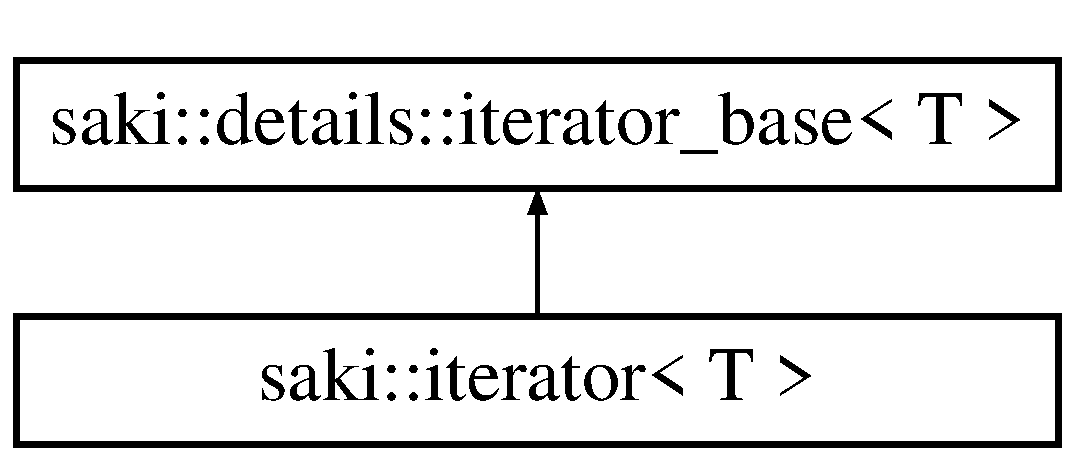
\includegraphics[height=2.000000cm]{classsaki_1_1iterator}
\end{center}
\end{figure}
\subsection*{公開メンバ関数}
\begin{DoxyCompactItemize}
\item 
constexpr \mbox{\hyperlink{classsaki_1_1iterator_aaf66a5b986033d29630294dd2646bec3}{iterator}} (T $\ast$pointer)
\end{DoxyCompactItemize}
\subsection*{その他の継承メンバ}


\subsection{詳解}
\subsubsection*{template$<$typename T$>$\newline
class saki\+::iterator$<$ T $>$}

ノーマルなイテレーター 

\subsection{構築子と解体子}
\mbox{\Hypertarget{classsaki_1_1iterator_aaf66a5b986033d29630294dd2646bec3}\label{classsaki_1_1iterator_aaf66a5b986033d29630294dd2646bec3}} 
\index{saki\+::iterator@{saki\+::iterator}!iterator@{iterator}}
\index{iterator@{iterator}!saki\+::iterator@{saki\+::iterator}}
\subsubsection{\texorpdfstring{iterator()}{iterator()}}
{\footnotesize\ttfamily template$<$typename T $>$ \\
constexpr \mbox{\hyperlink{classsaki_1_1iterator}{saki\+::iterator}}$<$ T $>$\+::\mbox{\hyperlink{classsaki_1_1iterator}{iterator}} (\begin{DoxyParamCaption}\item[{T $\ast$}]{pointer }\end{DoxyParamCaption})\hspace{0.3cm}{\ttfamily [inline]}, {\ttfamily [explicit]}}



このクラス詳解は次のファイルから抽出されました\+:\begin{DoxyCompactItemize}
\item 
C\+:/\+Users/tokir/\+Documents/\+Git\+Hub/\+Saki\+Cpp\+Library/saki/iterator/\mbox{\hyperlink{iterator_2iterator_8hpp}{iterator.\+hpp}}\end{DoxyCompactItemize}

\hypertarget{classsaki_1_1details_1_1iterator__base}{}\section{saki\+:\+:details\+:\+:iterator\+\_\+base$<$ T $>$ クラステンプレート}
\label{classsaki_1_1details_1_1iterator__base}\index{saki\+::details\+::iterator\+\_\+base$<$ T $>$@{saki\+::details\+::iterator\+\_\+base$<$ T $>$}}


イテレーターのベースクラス  




{\ttfamily \#include $<$iterator\+\_\+base.\+h$>$}

saki\+:\+:details\+:\+:iterator\+\_\+base$<$ T $>$ の継承関係図\begin{figure}[H]
\begin{center}
\leavevmode
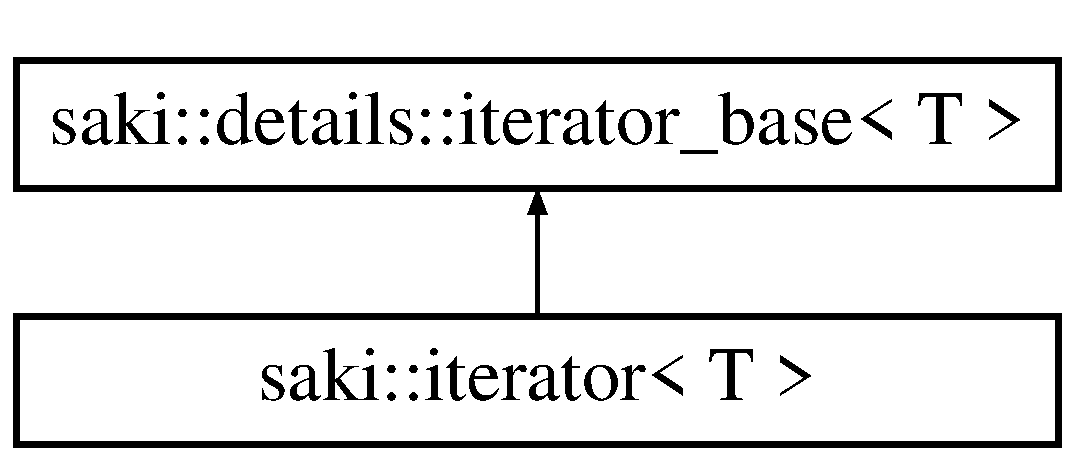
\includegraphics[height=2.000000cm]{classsaki_1_1details_1_1iterator__base}
\end{center}
\end{figure}
\subsection*{公開メンバ関数}
\begin{DoxyCompactItemize}
\item 
constexpr \mbox{\hyperlink{classsaki_1_1details_1_1iterator__base_a8fc711c3742cad39433fc3de560900f8}{iterator\+\_\+base}} (T $\ast$pointer)
\begin{DoxyCompactList}\small\item\em ポインタで初期化するコンストラクタ \end{DoxyCompactList}\item 
constexpr T \& \mbox{\hyperlink{classsaki_1_1details_1_1iterator__base_a621d7cd415fd0be31f666b54fadaf039}{operator$\ast$}} () const
\begin{DoxyCompactList}\small\item\em 間接参照演算子 \end{DoxyCompactList}\item 
constexpr T $\ast$ \mbox{\hyperlink{classsaki_1_1details_1_1iterator__base_a34d98882fa35d0c48ffe5a29c1a1f4cf}{operator-\/$>$}} () const
\begin{DoxyCompactList}\small\item\em アロー演算子 \end{DoxyCompactList}\item 
constexpr \mbox{\hyperlink{classsaki_1_1details_1_1iterator__base}{saki\+::details\+::iterator\+\_\+base}}$<$ T $>$ \& \mbox{\hyperlink{classsaki_1_1details_1_1iterator__base_a1539e90e42dd7208401df3ad5f6385b1}{operator++}} ()
\begin{DoxyCompactList}\small\item\em ++演算子(前置) \end{DoxyCompactList}\item 
constexpr \mbox{\hyperlink{classsaki_1_1details_1_1iterator__base}{saki\+::details\+::iterator\+\_\+base}}$<$ T $>$ \mbox{\hyperlink{classsaki_1_1details_1_1iterator__base_a47eb0dcb7d0467879a64eb252079d617}{operator++}} (int)
\begin{DoxyCompactList}\small\item\em ++演算子(後置) \end{DoxyCompactList}\item 
constexpr \mbox{\hyperlink{classsaki_1_1details_1_1iterator__base}{saki\+::details\+::iterator\+\_\+base}}$<$ T $>$ \& \mbox{\hyperlink{classsaki_1_1details_1_1iterator__base_abd955d1a288f42f0231f22c8a1e73040}{operator-\/-\/}} ()
\begin{DoxyCompactList}\small\item\em --演算子(前置) \end{DoxyCompactList}\item 
constexpr \mbox{\hyperlink{classsaki_1_1details_1_1iterator__base}{saki\+::details\+::iterator\+\_\+base}}$<$ T $>$ \mbox{\hyperlink{classsaki_1_1details_1_1iterator__base_a916d333d66267d52916eb442b092ed68}{operator-\/-\/}} (int)
\begin{DoxyCompactList}\small\item\em --演算子(後置) \end{DoxyCompactList}\end{DoxyCompactItemize}
\subsection*{限定公開変数類}
\begin{DoxyCompactItemize}
\item 
T $\ast$ \mbox{\hyperlink{classsaki_1_1details_1_1iterator__base_a26c42413a1c967669da4a52b1fe65f13}{itr}}
\end{DoxyCompactItemize}
\subsection*{フレンド}
\begin{DoxyCompactItemize}
\item 
{\footnotesize template$<$typename TT $>$ }\\constexpr bool \mbox{\hyperlink{classsaki_1_1details_1_1iterator__base_a6ac6c0419a9e263f0f89741137499a83}{operator==}} (const \mbox{\hyperlink{classsaki_1_1details_1_1iterator__base}{iterator\+\_\+base}}$<$ TT $>$ \&itr1, const \mbox{\hyperlink{classsaki_1_1details_1_1iterator__base}{iterator\+\_\+base}}$<$ TT $>$ \&itr2)
\item 
{\footnotesize template$<$typename TT $>$ }\\constexpr bool \mbox{\hyperlink{classsaki_1_1details_1_1iterator__base_a347d4c8755f8c350aa9c0151165549f2}{operator!=}} (const \mbox{\hyperlink{classsaki_1_1details_1_1iterator__base}{iterator\+\_\+base}}$<$ TT $>$ \&itr1, const \mbox{\hyperlink{classsaki_1_1details_1_1iterator__base}{iterator\+\_\+base}}$<$ TT $>$ \&itr2)
\end{DoxyCompactItemize}


\subsection{詳解}
\subsubsection*{template$<$typename T$>$\newline
class saki\+::details\+::iterator\+\_\+base$<$ T $>$}

イテレーターのベースクラス 

\subsection{構築子と解体子}
\mbox{\Hypertarget{classsaki_1_1details_1_1iterator__base_a8fc711c3742cad39433fc3de560900f8}\label{classsaki_1_1details_1_1iterator__base_a8fc711c3742cad39433fc3de560900f8}} 
\index{saki\+::details\+::iterator\+\_\+base@{saki\+::details\+::iterator\+\_\+base}!iterator\+\_\+base@{iterator\+\_\+base}}
\index{iterator\+\_\+base@{iterator\+\_\+base}!saki\+::details\+::iterator\+\_\+base@{saki\+::details\+::iterator\+\_\+base}}
\subsubsection{\texorpdfstring{iterator\+\_\+base()}{iterator\_base()}}
{\footnotesize\ttfamily template$<$typename T$>$ \\
constexpr \mbox{\hyperlink{classsaki_1_1details_1_1iterator__base}{saki\+::details\+::iterator\+\_\+base}}$<$ T $>$\+::\mbox{\hyperlink{classsaki_1_1details_1_1iterator__base}{iterator\+\_\+base}} (\begin{DoxyParamCaption}\item[{T $\ast$}]{pointer }\end{DoxyParamCaption})\hspace{0.3cm}{\ttfamily [inline]}, {\ttfamily [explicit]}}



ポインタで初期化するコンストラクタ 



\subsection{関数詳解}
\mbox{\Hypertarget{classsaki_1_1details_1_1iterator__base_a621d7cd415fd0be31f666b54fadaf039}\label{classsaki_1_1details_1_1iterator__base_a621d7cd415fd0be31f666b54fadaf039}} 
\index{saki\+::details\+::iterator\+\_\+base@{saki\+::details\+::iterator\+\_\+base}!operator$\ast$@{operator$\ast$}}
\index{operator$\ast$@{operator$\ast$}!saki\+::details\+::iterator\+\_\+base@{saki\+::details\+::iterator\+\_\+base}}
\subsubsection{\texorpdfstring{operator$\ast$()}{operator*()}}
{\footnotesize\ttfamily template$<$typename T$>$ \\
constexpr T\& \mbox{\hyperlink{classsaki_1_1details_1_1iterator__base}{saki\+::details\+::iterator\+\_\+base}}$<$ T $>$\+::operator$\ast$ (\begin{DoxyParamCaption}{ }\end{DoxyParamCaption}) const\hspace{0.3cm}{\ttfamily [inline]}}



間接参照演算子 

\mbox{\Hypertarget{classsaki_1_1details_1_1iterator__base_a1539e90e42dd7208401df3ad5f6385b1}\label{classsaki_1_1details_1_1iterator__base_a1539e90e42dd7208401df3ad5f6385b1}} 
\index{saki\+::details\+::iterator\+\_\+base@{saki\+::details\+::iterator\+\_\+base}!operator++@{operator++}}
\index{operator++@{operator++}!saki\+::details\+::iterator\+\_\+base@{saki\+::details\+::iterator\+\_\+base}}
\subsubsection{\texorpdfstring{operator++()}{operator++()}\hspace{0.1cm}{\footnotesize\ttfamily [1/2]}}
{\footnotesize\ttfamily template$<$typename T$>$ \\
constexpr \mbox{\hyperlink{classsaki_1_1details_1_1iterator__base}{saki\+::details\+::iterator\+\_\+base}}$<$T$>$\& \mbox{\hyperlink{classsaki_1_1details_1_1iterator__base}{saki\+::details\+::iterator\+\_\+base}}$<$ T $>$\+::operator++ (\begin{DoxyParamCaption}{ }\end{DoxyParamCaption})\hspace{0.3cm}{\ttfamily [inline]}}



++演算子(前置) 

\mbox{\Hypertarget{classsaki_1_1details_1_1iterator__base_a47eb0dcb7d0467879a64eb252079d617}\label{classsaki_1_1details_1_1iterator__base_a47eb0dcb7d0467879a64eb252079d617}} 
\index{saki\+::details\+::iterator\+\_\+base@{saki\+::details\+::iterator\+\_\+base}!operator++@{operator++}}
\index{operator++@{operator++}!saki\+::details\+::iterator\+\_\+base@{saki\+::details\+::iterator\+\_\+base}}
\subsubsection{\texorpdfstring{operator++()}{operator++()}\hspace{0.1cm}{\footnotesize\ttfamily [2/2]}}
{\footnotesize\ttfamily template$<$typename T$>$ \\
constexpr \mbox{\hyperlink{classsaki_1_1details_1_1iterator__base}{saki\+::details\+::iterator\+\_\+base}}$<$T$>$ \mbox{\hyperlink{classsaki_1_1details_1_1iterator__base}{saki\+::details\+::iterator\+\_\+base}}$<$ T $>$\+::operator++ (\begin{DoxyParamCaption}\item[{int}]{ }\end{DoxyParamCaption})\hspace{0.3cm}{\ttfamily [inline]}}



++演算子(後置) 

\mbox{\Hypertarget{classsaki_1_1details_1_1iterator__base_abd955d1a288f42f0231f22c8a1e73040}\label{classsaki_1_1details_1_1iterator__base_abd955d1a288f42f0231f22c8a1e73040}} 
\index{saki\+::details\+::iterator\+\_\+base@{saki\+::details\+::iterator\+\_\+base}!operator-\/-\/@{operator-\/-\/}}
\index{operator-\/-\/@{operator-\/-\/}!saki\+::details\+::iterator\+\_\+base@{saki\+::details\+::iterator\+\_\+base}}
\subsubsection{\texorpdfstring{operator-\/-\/()}{operator--()}\hspace{0.1cm}{\footnotesize\ttfamily [1/2]}}
{\footnotesize\ttfamily template$<$typename T$>$ \\
constexpr \mbox{\hyperlink{classsaki_1_1details_1_1iterator__base}{saki\+::details\+::iterator\+\_\+base}}$<$T$>$\& \mbox{\hyperlink{classsaki_1_1details_1_1iterator__base}{saki\+::details\+::iterator\+\_\+base}}$<$ T $>$\+::operator-\/-\/ (\begin{DoxyParamCaption}{ }\end{DoxyParamCaption})\hspace{0.3cm}{\ttfamily [inline]}}



--演算子(前置) 

\mbox{\Hypertarget{classsaki_1_1details_1_1iterator__base_a916d333d66267d52916eb442b092ed68}\label{classsaki_1_1details_1_1iterator__base_a916d333d66267d52916eb442b092ed68}} 
\index{saki\+::details\+::iterator\+\_\+base@{saki\+::details\+::iterator\+\_\+base}!operator-\/-\/@{operator-\/-\/}}
\index{operator-\/-\/@{operator-\/-\/}!saki\+::details\+::iterator\+\_\+base@{saki\+::details\+::iterator\+\_\+base}}
\subsubsection{\texorpdfstring{operator-\/-\/()}{operator--()}\hspace{0.1cm}{\footnotesize\ttfamily [2/2]}}
{\footnotesize\ttfamily template$<$typename T$>$ \\
constexpr \mbox{\hyperlink{classsaki_1_1details_1_1iterator__base}{saki\+::details\+::iterator\+\_\+base}}$<$T$>$ \mbox{\hyperlink{classsaki_1_1details_1_1iterator__base}{saki\+::details\+::iterator\+\_\+base}}$<$ T $>$\+::operator-\/-\/ (\begin{DoxyParamCaption}\item[{int}]{ }\end{DoxyParamCaption})\hspace{0.3cm}{\ttfamily [inline]}}



--演算子(後置) 

\mbox{\Hypertarget{classsaki_1_1details_1_1iterator__base_a34d98882fa35d0c48ffe5a29c1a1f4cf}\label{classsaki_1_1details_1_1iterator__base_a34d98882fa35d0c48ffe5a29c1a1f4cf}} 
\index{saki\+::details\+::iterator\+\_\+base@{saki\+::details\+::iterator\+\_\+base}!operator-\/$>$@{operator-\/$>$}}
\index{operator-\/$>$@{operator-\/$>$}!saki\+::details\+::iterator\+\_\+base@{saki\+::details\+::iterator\+\_\+base}}
\subsubsection{\texorpdfstring{operator-\/$>$()}{operator->()}}
{\footnotesize\ttfamily template$<$typename T$>$ \\
constexpr T$\ast$ \mbox{\hyperlink{classsaki_1_1details_1_1iterator__base}{saki\+::details\+::iterator\+\_\+base}}$<$ T $>$\+::operator-\/$>$ (\begin{DoxyParamCaption}{ }\end{DoxyParamCaption}) const\hspace{0.3cm}{\ttfamily [inline]}}



アロー演算子 



\subsection{フレンドと関連関数の詳解}
\mbox{\Hypertarget{classsaki_1_1details_1_1iterator__base_a347d4c8755f8c350aa9c0151165549f2}\label{classsaki_1_1details_1_1iterator__base_a347d4c8755f8c350aa9c0151165549f2}} 
\index{saki\+::details\+::iterator\+\_\+base@{saki\+::details\+::iterator\+\_\+base}!operator"!=@{operator"!=}}
\index{operator"!=@{operator"!=}!saki\+::details\+::iterator\+\_\+base@{saki\+::details\+::iterator\+\_\+base}}
\subsubsection{\texorpdfstring{operator"!=}{operator!=}}
{\footnotesize\ttfamily template$<$typename T$>$ \\
template$<$typename TT $>$ \\
constexpr bool operator!= (\begin{DoxyParamCaption}\item[{const \mbox{\hyperlink{classsaki_1_1details_1_1iterator__base}{iterator\+\_\+base}}$<$ TT $>$ \&}]{itr1,  }\item[{const \mbox{\hyperlink{classsaki_1_1details_1_1iterator__base}{iterator\+\_\+base}}$<$ TT $>$ \&}]{itr2 }\end{DoxyParamCaption})\hspace{0.3cm}{\ttfamily [friend]}}

\mbox{\Hypertarget{classsaki_1_1details_1_1iterator__base_a6ac6c0419a9e263f0f89741137499a83}\label{classsaki_1_1details_1_1iterator__base_a6ac6c0419a9e263f0f89741137499a83}} 
\index{saki\+::details\+::iterator\+\_\+base@{saki\+::details\+::iterator\+\_\+base}!operator==@{operator==}}
\index{operator==@{operator==}!saki\+::details\+::iterator\+\_\+base@{saki\+::details\+::iterator\+\_\+base}}
\subsubsection{\texorpdfstring{operator==}{operator==}}
{\footnotesize\ttfamily template$<$typename T$>$ \\
template$<$typename TT $>$ \\
constexpr bool operator== (\begin{DoxyParamCaption}\item[{const \mbox{\hyperlink{classsaki_1_1details_1_1iterator__base}{iterator\+\_\+base}}$<$ TT $>$ \&}]{itr1,  }\item[{const \mbox{\hyperlink{classsaki_1_1details_1_1iterator__base}{iterator\+\_\+base}}$<$ TT $>$ \&}]{itr2 }\end{DoxyParamCaption})\hspace{0.3cm}{\ttfamily [friend]}}



\subsection{メンバ詳解}
\mbox{\Hypertarget{classsaki_1_1details_1_1iterator__base_a26c42413a1c967669da4a52b1fe65f13}\label{classsaki_1_1details_1_1iterator__base_a26c42413a1c967669da4a52b1fe65f13}} 
\index{saki\+::details\+::iterator\+\_\+base@{saki\+::details\+::iterator\+\_\+base}!itr@{itr}}
\index{itr@{itr}!saki\+::details\+::iterator\+\_\+base@{saki\+::details\+::iterator\+\_\+base}}
\subsubsection{\texorpdfstring{itr}{itr}}
{\footnotesize\ttfamily template$<$typename T$>$ \\
T$\ast$ \mbox{\hyperlink{classsaki_1_1details_1_1iterator__base}{saki\+::details\+::iterator\+\_\+base}}$<$ T $>$\+::itr\hspace{0.3cm}{\ttfamily [protected]}}



このクラス詳解は次のファイルから抽出されました\+:\begin{DoxyCompactItemize}
\item 
C\+:/\+Users/tokir/\+Documents/\+Git\+Hub/\+Saki\+Cpp\+Library/saki/iterator/details/\mbox{\hyperlink{iterator__base_8h}{iterator\+\_\+base.\+h}}\end{DoxyCompactItemize}

\hypertarget{classsaki_1_1matrix}{}\section{saki\+:\+:matrix$<$ T $>$ クラステンプレート}
\label{classsaki_1_1matrix}\index{saki\+::matrix$<$ T $>$@{saki\+::matrix$<$ T $>$}}


行列  




{\ttfamily \#include $<$matrix\+\_\+math.\+hpp$>$}

\subsection*{公開メンバ関数}
\begin{DoxyCompactItemize}
\item 
constexpr \mbox{\hyperlink{classsaki_1_1matrix_aca5102e0cdaedc779d668597d03baf10}{matrix}} ()
\begin{DoxyCompactList}\small\item\em 引数なしコンストラクタ \end{DoxyCompactList}\item 
constexpr \mbox{\hyperlink{classsaki_1_1matrix_a55edebaa14a4a0ea6b6f263ebe9950f4}{matrix}} (const\+\_\+reference m00, const\+\_\+reference m01, const\+\_\+reference m02, const\+\_\+reference m03, const\+\_\+reference m10, const\+\_\+reference m11, const\+\_\+reference m12, const\+\_\+reference m13, const\+\_\+reference m20, const\+\_\+reference m21, const\+\_\+reference m22, const\+\_\+reference m23, const\+\_\+reference m30, const\+\_\+reference m31, const\+\_\+reference m32, const\+\_\+reference m33)
\begin{DoxyCompactList}\small\item\em 引数ありコンストラクタ \end{DoxyCompactList}\item 
{\footnotesize template$<$typename U $>$ }\\constexpr \mbox{\hyperlink{classsaki_1_1matrix_aadbe6027fea1fecafc641cd553855408}{matrix}} (const U arr\mbox{[}4\mbox{]}\mbox{[}4\mbox{]})
\begin{DoxyCompactList}\small\item\em 生配列からの初期化 \end{DoxyCompactList}\item 
{\footnotesize template$<$typename U1 , typename U2 , typename U3 , typename U4 $>$ }\\constexpr \mbox{\hyperlink{classsaki_1_1matrix_a05256e26b2d44fe97a157c5bb510cdaf}{matrix}} (const \mbox{\hyperlink{classsaki_1_1vector4}{saki\+::vector4}}$<$ U1 $>$ \&v1, const \mbox{\hyperlink{classsaki_1_1vector4}{saki\+::vector4}}$<$ U2 $>$ \&v2, const \mbox{\hyperlink{classsaki_1_1vector4}{saki\+::vector4}}$<$ U3 $>$ \&v3, const \mbox{\hyperlink{classsaki_1_1vector4}{saki\+::vector4}}$<$ U4 $>$ \&v4)
\begin{DoxyCompactList}\small\item\em vector4での初期化 \end{DoxyCompactList}\item 
\mbox{\hyperlink{classsaki_1_1matrix_ad17aa0026d1a795166d6654b1df702c3}{matrix}} (const \mbox{\hyperlink{classsaki_1_1matrix}{matrix}}$<$ value\+\_\+type $>$ \&)=default
\item 
\mbox{\hyperlink{classsaki_1_1matrix}{matrix}}$<$ value\+\_\+type $>$ \& \mbox{\hyperlink{classsaki_1_1matrix_a38c5f7e666e3888d90b1c4017219f53f}{operator=}} (const \mbox{\hyperlink{classsaki_1_1matrix}{matrix}}$<$ value\+\_\+type $>$ \&)=default
\item 
\mbox{\hyperlink{classsaki_1_1matrix_a16b927b776bc7454ebbf984b7f93c23e}{matrix}} (\mbox{\hyperlink{classsaki_1_1matrix}{matrix}}$<$ value\+\_\+type $>$ \&\&) noexcept=default
\item 
\mbox{\hyperlink{classsaki_1_1matrix}{matrix}}$<$ value\+\_\+type $>$ \& \mbox{\hyperlink{classsaki_1_1matrix_a06a7330daf074554dada53978e3ccd55}{operator=}} (\mbox{\hyperlink{classsaki_1_1matrix}{matrix}}$<$ value\+\_\+type $>$ \&\&) noexcept=default
\item 
\mbox{\hyperlink{classsaki_1_1matrix_a6fe9a4d52c93051ecdb1075abe5a272b}{$\sim$matrix}} () noexcept=default
\item 
{\footnotesize template$<$typename U  = value\+\_\+type$>$ }\\auto \mbox{\hyperlink{classsaki_1_1matrix_ad004cb2830b0c22778b99b57fcbde8df}{operator+=}} (const \mbox{\hyperlink{classsaki_1_1matrix}{saki\+::matrix}}$<$ U $>$ \&other)
\begin{DoxyCompactList}\small\item\em +=演算子 \end{DoxyCompactList}\item 
{\footnotesize template$<$typename U  = value\+\_\+type$>$ }\\auto \mbox{\hyperlink{classsaki_1_1matrix_ae7c736de15ce97ad5d41193beeecf18d}{operator-\/=}} (const \mbox{\hyperlink{classsaki_1_1matrix}{saki\+::matrix}}$<$ U $>$ \&other)
\begin{DoxyCompactList}\small\item\em -\/=演算子 \end{DoxyCompactList}\item 
{\footnotesize template$<$typename U  = value\+\_\+type$>$ }\\auto \mbox{\hyperlink{classsaki_1_1matrix_ade74f7e19240123da31171ca469246e7}{operator$\ast$=}} (const U \&scalar)
\begin{DoxyCompactList}\small\item\em $\ast$=演算子(スカラ) \end{DoxyCompactList}\item 
{\footnotesize template$<$typename U  = value\+\_\+type$>$ }\\auto \mbox{\hyperlink{classsaki_1_1matrix_acb32e13e61d31a15341fbf2996f6428b}{operator$\ast$=}} (const \mbox{\hyperlink{classsaki_1_1matrix}{saki\+::matrix}}$<$ U $>$ \&other)
\begin{DoxyCompactList}\small\item\em $\ast$=演算子(行列) \end{DoxyCompactList}\item 
{\footnotesize template$<$typename U  = value\+\_\+type$>$ }\\auto \mbox{\hyperlink{classsaki_1_1matrix_af70c929f45bbea2192aab47d49882d3c}{operator/=}} (const U \&scalar)
\begin{DoxyCompactList}\small\item\em /=演算子(スカラ) \end{DoxyCompactList}\item 
constexpr \mbox{\hyperlink{classsaki_1_1matrix}{saki\+::matrix}}$<$ value\+\_\+type $>$ \mbox{\hyperlink{classsaki_1_1matrix_ada12f77277660f640f46c9bc7e67c04c}{operator+}} () const
\begin{DoxyCompactList}\small\item\em 単項+演算子 \end{DoxyCompactList}\item 
constexpr \mbox{\hyperlink{classsaki_1_1matrix}{saki\+::matrix}}$<$ value\+\_\+type $>$ \mbox{\hyperlink{classsaki_1_1matrix_a11aa55aa5c0efdc11c93c6a80188ac62}{operator-\/}} () const
\begin{DoxyCompactList}\small\item\em 単項-\/演算子 \end{DoxyCompactList}\item 
constexpr \mbox{\hyperlink{classsaki_1_1array}{saki\+::array}}$<$ value\+\_\+type, 4 $>$ \& \mbox{\hyperlink{classsaki_1_1matrix_a9438f349876b7932a5c3c58a713e3e00}{operator\mbox{[}$\,$\mbox{]}}} (const size\+\_\+t index)
\begin{DoxyCompactList}\small\item\em \mbox{[}\mbox{]}演算子 \end{DoxyCompactList}\item 
constexpr const \mbox{\hyperlink{classsaki_1_1array}{saki\+::array}}$<$ value\+\_\+type, 4 $>$ \& \mbox{\hyperlink{classsaki_1_1matrix_a1a326fe310df8da04d32200dd6ae1e64}{operator\mbox{[}$\,$\mbox{]}}} (const size\+\_\+t index) const
\begin{DoxyCompactList}\small\item\em \mbox{[}\mbox{]}演算子(constexpr) \end{DoxyCompactList}\item 
void \mbox{\hyperlink{classsaki_1_1matrix_a9f7f8909ee94f44e91faca871f57b936}{identity}} ()
\begin{DoxyCompactList}\small\item\em 単位行列に変換 \end{DoxyCompactList}\item 
void \mbox{\hyperlink{classsaki_1_1matrix_a95e01e24e45757c1e45b5af25273a8fa}{transpose}} ()
\begin{DoxyCompactList}\small\item\em 転置行列に変換 \end{DoxyCompactList}\end{DoxyCompactItemize}


\subsection{詳解}
\subsubsection*{template$<$typename T$>$\newline
class saki\+::matrix$<$ T $>$}

行列 

\subsection{構築子と解体子}
\mbox{\Hypertarget{classsaki_1_1matrix_aca5102e0cdaedc779d668597d03baf10}\label{classsaki_1_1matrix_aca5102e0cdaedc779d668597d03baf10}} 
\index{saki\+::matrix@{saki\+::matrix}!matrix@{matrix}}
\index{matrix@{matrix}!saki\+::matrix@{saki\+::matrix}}
\subsubsection{\texorpdfstring{matrix()}{matrix()}\hspace{0.1cm}{\footnotesize\ttfamily [1/6]}}
{\footnotesize\ttfamily template$<$typename T$>$ \\
constexpr \mbox{\hyperlink{classsaki_1_1matrix}{saki\+::matrix}}$<$ T $>$\+::\mbox{\hyperlink{classsaki_1_1matrix}{matrix}} (\begin{DoxyParamCaption}{ }\end{DoxyParamCaption})\hspace{0.3cm}{\ttfamily [inline]}}



引数なしコンストラクタ 

Identity初期化 \mbox{\Hypertarget{classsaki_1_1matrix_a55edebaa14a4a0ea6b6f263ebe9950f4}\label{classsaki_1_1matrix_a55edebaa14a4a0ea6b6f263ebe9950f4}} 
\index{saki\+::matrix@{saki\+::matrix}!matrix@{matrix}}
\index{matrix@{matrix}!saki\+::matrix@{saki\+::matrix}}
\subsubsection{\texorpdfstring{matrix()}{matrix()}\hspace{0.1cm}{\footnotesize\ttfamily [2/6]}}
{\footnotesize\ttfamily template$<$typename T$>$ \\
constexpr \mbox{\hyperlink{classsaki_1_1matrix}{saki\+::matrix}}$<$ T $>$\+::\mbox{\hyperlink{classsaki_1_1matrix}{matrix}} (\begin{DoxyParamCaption}\item[{const\+\_\+reference}]{m00,  }\item[{const\+\_\+reference}]{m01,  }\item[{const\+\_\+reference}]{m02,  }\item[{const\+\_\+reference}]{m03,  }\item[{const\+\_\+reference}]{m10,  }\item[{const\+\_\+reference}]{m11,  }\item[{const\+\_\+reference}]{m12,  }\item[{const\+\_\+reference}]{m13,  }\item[{const\+\_\+reference}]{m20,  }\item[{const\+\_\+reference}]{m21,  }\item[{const\+\_\+reference}]{m22,  }\item[{const\+\_\+reference}]{m23,  }\item[{const\+\_\+reference}]{m30,  }\item[{const\+\_\+reference}]{m31,  }\item[{const\+\_\+reference}]{m32,  }\item[{const\+\_\+reference}]{m33 }\end{DoxyParamCaption})\hspace{0.3cm}{\ttfamily [inline]}}



引数ありコンストラクタ 

\mbox{\Hypertarget{classsaki_1_1matrix_aadbe6027fea1fecafc641cd553855408}\label{classsaki_1_1matrix_aadbe6027fea1fecafc641cd553855408}} 
\index{saki\+::matrix@{saki\+::matrix}!matrix@{matrix}}
\index{matrix@{matrix}!saki\+::matrix@{saki\+::matrix}}
\subsubsection{\texorpdfstring{matrix()}{matrix()}\hspace{0.1cm}{\footnotesize\ttfamily [3/6]}}
{\footnotesize\ttfamily template$<$typename T$>$ \\
template$<$typename U $>$ \\
constexpr \mbox{\hyperlink{classsaki_1_1matrix}{saki\+::matrix}}$<$ T $>$\+::\mbox{\hyperlink{classsaki_1_1matrix}{matrix}} (\begin{DoxyParamCaption}\item[{const U}]{arr\mbox{[}4\mbox{]}\mbox{[}4\mbox{]} }\end{DoxyParamCaption})\hspace{0.3cm}{\ttfamily [inline]}, {\ttfamily [explicit]}}



生配列からの初期化 


\begin{DoxyParams}{引数}
{\em arr} & 4$\ast$4の配列 \\
\hline
\end{DoxyParams}
\mbox{\Hypertarget{classsaki_1_1matrix_a05256e26b2d44fe97a157c5bb510cdaf}\label{classsaki_1_1matrix_a05256e26b2d44fe97a157c5bb510cdaf}} 
\index{saki\+::matrix@{saki\+::matrix}!matrix@{matrix}}
\index{matrix@{matrix}!saki\+::matrix@{saki\+::matrix}}
\subsubsection{\texorpdfstring{matrix()}{matrix()}\hspace{0.1cm}{\footnotesize\ttfamily [4/6]}}
{\footnotesize\ttfamily template$<$typename T$>$ \\
template$<$typename U1 , typename U2 , typename U3 , typename U4 $>$ \\
constexpr \mbox{\hyperlink{classsaki_1_1matrix}{saki\+::matrix}}$<$ T $>$\+::\mbox{\hyperlink{classsaki_1_1matrix}{matrix}} (\begin{DoxyParamCaption}\item[{const \mbox{\hyperlink{classsaki_1_1vector4}{saki\+::vector4}}$<$ U1 $>$ \&}]{v1,  }\item[{const \mbox{\hyperlink{classsaki_1_1vector4}{saki\+::vector4}}$<$ U2 $>$ \&}]{v2,  }\item[{const \mbox{\hyperlink{classsaki_1_1vector4}{saki\+::vector4}}$<$ U3 $>$ \&}]{v3,  }\item[{const \mbox{\hyperlink{classsaki_1_1vector4}{saki\+::vector4}}$<$ U4 $>$ \&}]{v4 }\end{DoxyParamCaption})\hspace{0.3cm}{\ttfamily [inline]}}



vector4での初期化 


\begin{DoxyParams}{引数}
{\em v1} & 1行目 \\
\hline
{\em v2} & 2行目 \\
\hline
{\em v3} & 3行目 \\
\hline
{\em v4} & 4行目 \\
\hline
\end{DoxyParams}
\mbox{\Hypertarget{classsaki_1_1matrix_ad17aa0026d1a795166d6654b1df702c3}\label{classsaki_1_1matrix_ad17aa0026d1a795166d6654b1df702c3}} 
\index{saki\+::matrix@{saki\+::matrix}!matrix@{matrix}}
\index{matrix@{matrix}!saki\+::matrix@{saki\+::matrix}}
\subsubsection{\texorpdfstring{matrix()}{matrix()}\hspace{0.1cm}{\footnotesize\ttfamily [5/6]}}
{\footnotesize\ttfamily template$<$typename T$>$ \\
\mbox{\hyperlink{classsaki_1_1matrix}{saki\+::matrix}}$<$ T $>$\+::\mbox{\hyperlink{classsaki_1_1matrix}{matrix}} (\begin{DoxyParamCaption}\item[{const \mbox{\hyperlink{classsaki_1_1matrix}{matrix}}$<$ value\+\_\+type $>$ \&}]{ }\end{DoxyParamCaption})\hspace{0.3cm}{\ttfamily [default]}}

\mbox{\Hypertarget{classsaki_1_1matrix_a16b927b776bc7454ebbf984b7f93c23e}\label{classsaki_1_1matrix_a16b927b776bc7454ebbf984b7f93c23e}} 
\index{saki\+::matrix@{saki\+::matrix}!matrix@{matrix}}
\index{matrix@{matrix}!saki\+::matrix@{saki\+::matrix}}
\subsubsection{\texorpdfstring{matrix()}{matrix()}\hspace{0.1cm}{\footnotesize\ttfamily [6/6]}}
{\footnotesize\ttfamily template$<$typename T$>$ \\
\mbox{\hyperlink{classsaki_1_1matrix}{saki\+::matrix}}$<$ T $>$\+::\mbox{\hyperlink{classsaki_1_1matrix}{matrix}} (\begin{DoxyParamCaption}\item[{\mbox{\hyperlink{classsaki_1_1matrix}{matrix}}$<$ value\+\_\+type $>$ \&\&}]{ }\end{DoxyParamCaption})\hspace{0.3cm}{\ttfamily [default]}, {\ttfamily [noexcept]}}

\mbox{\Hypertarget{classsaki_1_1matrix_a6fe9a4d52c93051ecdb1075abe5a272b}\label{classsaki_1_1matrix_a6fe9a4d52c93051ecdb1075abe5a272b}} 
\index{saki\+::matrix@{saki\+::matrix}!````~matrix@{$\sim$matrix}}
\index{````~matrix@{$\sim$matrix}!saki\+::matrix@{saki\+::matrix}}
\subsubsection{\texorpdfstring{$\sim$matrix()}{~matrix()}}
{\footnotesize\ttfamily template$<$typename T$>$ \\
\mbox{\hyperlink{classsaki_1_1matrix}{saki\+::matrix}}$<$ T $>$\+::$\sim$\mbox{\hyperlink{classsaki_1_1matrix}{matrix}} (\begin{DoxyParamCaption}{ }\end{DoxyParamCaption})\hspace{0.3cm}{\ttfamily [default]}, {\ttfamily [noexcept]}}



\subsection{関数詳解}
\mbox{\Hypertarget{classsaki_1_1matrix_a9f7f8909ee94f44e91faca871f57b936}\label{classsaki_1_1matrix_a9f7f8909ee94f44e91faca871f57b936}} 
\index{saki\+::matrix@{saki\+::matrix}!identity@{identity}}
\index{identity@{identity}!saki\+::matrix@{saki\+::matrix}}
\subsubsection{\texorpdfstring{identity()}{identity()}}
{\footnotesize\ttfamily template$<$typename T$>$ \\
void \mbox{\hyperlink{classsaki_1_1matrix}{saki\+::matrix}}$<$ T $>$\+::identity (\begin{DoxyParamCaption}{ }\end{DoxyParamCaption})\hspace{0.3cm}{\ttfamily [inline]}}



単位行列に変換 

\mbox{\Hypertarget{classsaki_1_1matrix_ade74f7e19240123da31171ca469246e7}\label{classsaki_1_1matrix_ade74f7e19240123da31171ca469246e7}} 
\index{saki\+::matrix@{saki\+::matrix}!operator$\ast$=@{operator$\ast$=}}
\index{operator$\ast$=@{operator$\ast$=}!saki\+::matrix@{saki\+::matrix}}
\subsubsection{\texorpdfstring{operator$\ast$=()}{operator*=()}\hspace{0.1cm}{\footnotesize\ttfamily [1/2]}}
{\footnotesize\ttfamily template$<$typename T$>$ \\
template$<$typename U  = value\+\_\+type$>$ \\
auto \mbox{\hyperlink{classsaki_1_1matrix}{saki\+::matrix}}$<$ T $>$\+::operator$\ast$= (\begin{DoxyParamCaption}\item[{const U \&}]{scalar }\end{DoxyParamCaption})\hspace{0.3cm}{\ttfamily [inline]}}



$\ast$=演算子(スカラ) 

\mbox{\Hypertarget{classsaki_1_1matrix_acb32e13e61d31a15341fbf2996f6428b}\label{classsaki_1_1matrix_acb32e13e61d31a15341fbf2996f6428b}} 
\index{saki\+::matrix@{saki\+::matrix}!operator$\ast$=@{operator$\ast$=}}
\index{operator$\ast$=@{operator$\ast$=}!saki\+::matrix@{saki\+::matrix}}
\subsubsection{\texorpdfstring{operator$\ast$=()}{operator*=()}\hspace{0.1cm}{\footnotesize\ttfamily [2/2]}}
{\footnotesize\ttfamily template$<$typename T$>$ \\
template$<$typename U  = value\+\_\+type$>$ \\
auto \mbox{\hyperlink{classsaki_1_1matrix}{saki\+::matrix}}$<$ T $>$\+::operator$\ast$= (\begin{DoxyParamCaption}\item[{const \mbox{\hyperlink{classsaki_1_1matrix}{saki\+::matrix}}$<$ U $>$ \&}]{other }\end{DoxyParamCaption})\hspace{0.3cm}{\ttfamily [inline]}}



$\ast$=演算子(行列) 

\mbox{\Hypertarget{classsaki_1_1matrix_ada12f77277660f640f46c9bc7e67c04c}\label{classsaki_1_1matrix_ada12f77277660f640f46c9bc7e67c04c}} 
\index{saki\+::matrix@{saki\+::matrix}!operator+@{operator+}}
\index{operator+@{operator+}!saki\+::matrix@{saki\+::matrix}}
\subsubsection{\texorpdfstring{operator+()}{operator+()}}
{\footnotesize\ttfamily template$<$typename T$>$ \\
constexpr \mbox{\hyperlink{classsaki_1_1matrix}{saki\+::matrix}}$<$value\+\_\+type$>$ \mbox{\hyperlink{classsaki_1_1matrix}{saki\+::matrix}}$<$ T $>$\+::operator+ (\begin{DoxyParamCaption}{ }\end{DoxyParamCaption}) const\hspace{0.3cm}{\ttfamily [inline]}}



単項+演算子 

\mbox{\Hypertarget{classsaki_1_1matrix_ad004cb2830b0c22778b99b57fcbde8df}\label{classsaki_1_1matrix_ad004cb2830b0c22778b99b57fcbde8df}} 
\index{saki\+::matrix@{saki\+::matrix}!operator+=@{operator+=}}
\index{operator+=@{operator+=}!saki\+::matrix@{saki\+::matrix}}
\subsubsection{\texorpdfstring{operator+=()}{operator+=()}}
{\footnotesize\ttfamily template$<$typename T$>$ \\
template$<$typename U  = value\+\_\+type$>$ \\
auto \mbox{\hyperlink{classsaki_1_1matrix}{saki\+::matrix}}$<$ T $>$\+::operator+= (\begin{DoxyParamCaption}\item[{const \mbox{\hyperlink{classsaki_1_1matrix}{saki\+::matrix}}$<$ U $>$ \&}]{other }\end{DoxyParamCaption})\hspace{0.3cm}{\ttfamily [inline]}}



+=演算子 

\mbox{\Hypertarget{classsaki_1_1matrix_a11aa55aa5c0efdc11c93c6a80188ac62}\label{classsaki_1_1matrix_a11aa55aa5c0efdc11c93c6a80188ac62}} 
\index{saki\+::matrix@{saki\+::matrix}!operator-\/@{operator-\/}}
\index{operator-\/@{operator-\/}!saki\+::matrix@{saki\+::matrix}}
\subsubsection{\texorpdfstring{operator-\/()}{operator-()}}
{\footnotesize\ttfamily template$<$typename T$>$ \\
constexpr \mbox{\hyperlink{classsaki_1_1matrix}{saki\+::matrix}}$<$value\+\_\+type$>$ \mbox{\hyperlink{classsaki_1_1matrix}{saki\+::matrix}}$<$ T $>$\+::operator-\/ (\begin{DoxyParamCaption}{ }\end{DoxyParamCaption}) const\hspace{0.3cm}{\ttfamily [inline]}}



単項-\/演算子 

\mbox{\Hypertarget{classsaki_1_1matrix_ae7c736de15ce97ad5d41193beeecf18d}\label{classsaki_1_1matrix_ae7c736de15ce97ad5d41193beeecf18d}} 
\index{saki\+::matrix@{saki\+::matrix}!operator-\/=@{operator-\/=}}
\index{operator-\/=@{operator-\/=}!saki\+::matrix@{saki\+::matrix}}
\subsubsection{\texorpdfstring{operator-\/=()}{operator-=()}}
{\footnotesize\ttfamily template$<$typename T$>$ \\
template$<$typename U  = value\+\_\+type$>$ \\
auto \mbox{\hyperlink{classsaki_1_1matrix}{saki\+::matrix}}$<$ T $>$\+::operator-\/= (\begin{DoxyParamCaption}\item[{const \mbox{\hyperlink{classsaki_1_1matrix}{saki\+::matrix}}$<$ U $>$ \&}]{other }\end{DoxyParamCaption})\hspace{0.3cm}{\ttfamily [inline]}}



-\/=演算子 

\mbox{\Hypertarget{classsaki_1_1matrix_af70c929f45bbea2192aab47d49882d3c}\label{classsaki_1_1matrix_af70c929f45bbea2192aab47d49882d3c}} 
\index{saki\+::matrix@{saki\+::matrix}!operator/=@{operator/=}}
\index{operator/=@{operator/=}!saki\+::matrix@{saki\+::matrix}}
\subsubsection{\texorpdfstring{operator/=()}{operator/=()}}
{\footnotesize\ttfamily template$<$typename T$>$ \\
template$<$typename U  = value\+\_\+type$>$ \\
auto \mbox{\hyperlink{classsaki_1_1matrix}{saki\+::matrix}}$<$ T $>$\+::operator/= (\begin{DoxyParamCaption}\item[{const U \&}]{scalar }\end{DoxyParamCaption})\hspace{0.3cm}{\ttfamily [inline]}}



/=演算子(スカラ) 

\mbox{\Hypertarget{classsaki_1_1matrix_a38c5f7e666e3888d90b1c4017219f53f}\label{classsaki_1_1matrix_a38c5f7e666e3888d90b1c4017219f53f}} 
\index{saki\+::matrix@{saki\+::matrix}!operator=@{operator=}}
\index{operator=@{operator=}!saki\+::matrix@{saki\+::matrix}}
\subsubsection{\texorpdfstring{operator=()}{operator=()}\hspace{0.1cm}{\footnotesize\ttfamily [1/2]}}
{\footnotesize\ttfamily template$<$typename T$>$ \\
\mbox{\hyperlink{classsaki_1_1matrix}{matrix}}$<$value\+\_\+type$>$\& \mbox{\hyperlink{classsaki_1_1matrix}{saki\+::matrix}}$<$ T $>$\+::operator= (\begin{DoxyParamCaption}\item[{const \mbox{\hyperlink{classsaki_1_1matrix}{matrix}}$<$ value\+\_\+type $>$ \&}]{ }\end{DoxyParamCaption})\hspace{0.3cm}{\ttfamily [default]}}

\mbox{\Hypertarget{classsaki_1_1matrix_a06a7330daf074554dada53978e3ccd55}\label{classsaki_1_1matrix_a06a7330daf074554dada53978e3ccd55}} 
\index{saki\+::matrix@{saki\+::matrix}!operator=@{operator=}}
\index{operator=@{operator=}!saki\+::matrix@{saki\+::matrix}}
\subsubsection{\texorpdfstring{operator=()}{operator=()}\hspace{0.1cm}{\footnotesize\ttfamily [2/2]}}
{\footnotesize\ttfamily template$<$typename T$>$ \\
\mbox{\hyperlink{classsaki_1_1matrix}{matrix}}$<$value\+\_\+type$>$\& \mbox{\hyperlink{classsaki_1_1matrix}{saki\+::matrix}}$<$ T $>$\+::operator= (\begin{DoxyParamCaption}\item[{\mbox{\hyperlink{classsaki_1_1matrix}{matrix}}$<$ value\+\_\+type $>$ \&\&}]{ }\end{DoxyParamCaption})\hspace{0.3cm}{\ttfamily [default]}, {\ttfamily [noexcept]}}

\mbox{\Hypertarget{classsaki_1_1matrix_a9438f349876b7932a5c3c58a713e3e00}\label{classsaki_1_1matrix_a9438f349876b7932a5c3c58a713e3e00}} 
\index{saki\+::matrix@{saki\+::matrix}!operator\mbox{[}\mbox{]}@{operator[]}}
\index{operator\mbox{[}\mbox{]}@{operator[]}!saki\+::matrix@{saki\+::matrix}}
\subsubsection{\texorpdfstring{operator[]()}{operator[]()}\hspace{0.1cm}{\footnotesize\ttfamily [1/2]}}
{\footnotesize\ttfamily template$<$typename T$>$ \\
constexpr \mbox{\hyperlink{classsaki_1_1array}{saki\+::array}}$<$value\+\_\+type, 4$>$\& \mbox{\hyperlink{classsaki_1_1matrix}{saki\+::matrix}}$<$ T $>$\+::operator\mbox{[}$\,$\mbox{]} (\begin{DoxyParamCaption}\item[{const size\+\_\+t}]{index }\end{DoxyParamCaption})\hspace{0.3cm}{\ttfamily [inline]}}



\mbox{[}\mbox{]}演算子 

\mbox{\Hypertarget{classsaki_1_1matrix_a1a326fe310df8da04d32200dd6ae1e64}\label{classsaki_1_1matrix_a1a326fe310df8da04d32200dd6ae1e64}} 
\index{saki\+::matrix@{saki\+::matrix}!operator\mbox{[}\mbox{]}@{operator[]}}
\index{operator\mbox{[}\mbox{]}@{operator[]}!saki\+::matrix@{saki\+::matrix}}
\subsubsection{\texorpdfstring{operator[]()}{operator[]()}\hspace{0.1cm}{\footnotesize\ttfamily [2/2]}}
{\footnotesize\ttfamily template$<$typename T$>$ \\
constexpr const \mbox{\hyperlink{classsaki_1_1array}{saki\+::array}}$<$value\+\_\+type, 4$>$\& \mbox{\hyperlink{classsaki_1_1matrix}{saki\+::matrix}}$<$ T $>$\+::operator\mbox{[}$\,$\mbox{]} (\begin{DoxyParamCaption}\item[{const size\+\_\+t}]{index }\end{DoxyParamCaption}) const\hspace{0.3cm}{\ttfamily [inline]}}



\mbox{[}\mbox{]}演算子(constexpr) 

\mbox{\Hypertarget{classsaki_1_1matrix_a95e01e24e45757c1e45b5af25273a8fa}\label{classsaki_1_1matrix_a95e01e24e45757c1e45b5af25273a8fa}} 
\index{saki\+::matrix@{saki\+::matrix}!transpose@{transpose}}
\index{transpose@{transpose}!saki\+::matrix@{saki\+::matrix}}
\subsubsection{\texorpdfstring{transpose()}{transpose()}}
{\footnotesize\ttfamily template$<$typename T$>$ \\
void \mbox{\hyperlink{classsaki_1_1matrix}{saki\+::matrix}}$<$ T $>$\+::transpose (\begin{DoxyParamCaption}{ }\end{DoxyParamCaption})\hspace{0.3cm}{\ttfamily [inline]}}



転置行列に変換 



このクラス詳解は次のファイルから抽出されました\+:\begin{DoxyCompactItemize}
\item 
C\+:/\+Users/tokir/\+Documents/\+Git\+Hub/\+Saki\+Cpp\+Library/saki/matrix/details/\mbox{\hyperlink{matrix__math_8hpp}{matrix\+\_\+math.\+hpp}}\item 
C\+:/\+Users/tokir/\+Documents/\+Git\+Hub/\+Saki\+Cpp\+Library/saki/matrix/\mbox{\hyperlink{matrix_2matrix_8hpp}{matrix.\+hpp}}\end{DoxyCompactItemize}

\hypertarget{classsaki_1_1_multiple_separation}{}\section{saki\+:\+:Multiple\+Separation クラス}
\label{classsaki_1_1_multiple_separation}\index{saki\+::\+Multiple\+Separation@{saki\+::\+Multiple\+Separation}}


split関数で利用する、区切り文字を複数指定できるクラス  




{\ttfamily \#include $<$multiple\+\_\+separation.\+h$>$}

\subsection*{公開メンバ関数}
\begin{DoxyCompactItemize}
\item 
{\footnotesize template$<$typename ... T$>$ }\\\mbox{\hyperlink{classsaki_1_1_multiple_separation_a5dd228278057afbf2f1779891de59c63}{Multiple\+Separation}} (const T \&...t)
\begin{DoxyCompactList}\small\item\em コンストラクタ \end{DoxyCompactList}\item 
bool \mbox{\hyperlink{classsaki_1_1_multiple_separation_a27725149daca02b021edf69c58bbe140}{check}} (const char c)
\begin{DoxyCompactList}\small\item\em 渡された引数が区切り文字かチェックする \end{DoxyCompactList}\end{DoxyCompactItemize}


\subsection{詳解}
split関数で利用する、区切り文字を複数指定できるクラス 

\subsection{構築子と解体子}
\mbox{\Hypertarget{classsaki_1_1_multiple_separation_a5dd228278057afbf2f1779891de59c63}\label{classsaki_1_1_multiple_separation_a5dd228278057afbf2f1779891de59c63}} 
\index{saki\+::\+Multiple\+Separation@{saki\+::\+Multiple\+Separation}!Multiple\+Separation@{Multiple\+Separation}}
\index{Multiple\+Separation@{Multiple\+Separation}!saki\+::\+Multiple\+Separation@{saki\+::\+Multiple\+Separation}}
\subsubsection{\texorpdfstring{Multiple\+Separation()}{MultipleSeparation()}}
{\footnotesize\ttfamily template$<$typename ... T$>$ \\
saki\+::\+Multiple\+Separation\+::\+Multiple\+Separation (\begin{DoxyParamCaption}\item[{const T \&...}]{t }\end{DoxyParamCaption})\hspace{0.3cm}{\ttfamily [inline]}, {\ttfamily [explicit]}}



コンストラクタ 


\begin{DoxyParams}{引数}
{\em t} & 区切り文字 \\
\hline
\end{DoxyParams}


\subsection{関数詳解}
\mbox{\Hypertarget{classsaki_1_1_multiple_separation_a27725149daca02b021edf69c58bbe140}\label{classsaki_1_1_multiple_separation_a27725149daca02b021edf69c58bbe140}} 
\index{saki\+::\+Multiple\+Separation@{saki\+::\+Multiple\+Separation}!check@{check}}
\index{check@{check}!saki\+::\+Multiple\+Separation@{saki\+::\+Multiple\+Separation}}
\subsubsection{\texorpdfstring{check()}{check()}}
{\footnotesize\ttfamily bool saki\+::\+Multiple\+Separation\+::check (\begin{DoxyParamCaption}\item[{const char}]{c }\end{DoxyParamCaption})\hspace{0.3cm}{\ttfamily [inline]}}



渡された引数が区切り文字かチェックする 


\begin{DoxyParams}{引数}
{\em c} & 判定する文字\\
\hline
\end{DoxyParams}
bool \mbox{\hyperlink{classsaki_1_1_multiple_separation_a27725149daca02b021edf69c58bbe140}{check(char)}}という形にしなけらばならない 

このクラス詳解は次のファイルから抽出されました\+:\begin{DoxyCompactItemize}
\item 
C\+:/\+Users/tokir/\+Documents/\+Git\+Hub/\+Saki\+Cpp\+Library/saki/split/details/\mbox{\hyperlink{multiple__separation_8h}{multiple\+\_\+separation.\+h}}\end{DoxyCompactItemize}

\hypertarget{structsaki_1_1multiplication}{}\section{saki\+:\+:multiplication 構造体}
\label{structsaki_1_1multiplication}\index{saki\+::multiplication@{saki\+::multiplication}}


掛け算のconstexpr対応した関数オブジェクト  




{\ttfamily \#include $<$multiplication.\+h$>$}

\subsection*{公開メンバ関数}
\begin{DoxyCompactItemize}
\item 
{\footnotesize template$<$typename T1 , typename T2 $>$ }\\constexpr auto \mbox{\hyperlink{structsaki_1_1multiplication_ad7c9cfc08911b6db3ea95d4cfd5ffa7f}{operator()}} (const T1 \&t1, const T2 \&t2) const
\end{DoxyCompactItemize}


\subsection{詳解}
掛け算のconstexpr対応した関数オブジェクト 

\subsection{関数詳解}
\mbox{\Hypertarget{structsaki_1_1multiplication_ad7c9cfc08911b6db3ea95d4cfd5ffa7f}\label{structsaki_1_1multiplication_ad7c9cfc08911b6db3ea95d4cfd5ffa7f}} 
\index{saki\+::multiplication@{saki\+::multiplication}!operator()@{operator()}}
\index{operator()@{operator()}!saki\+::multiplication@{saki\+::multiplication}}
\subsubsection{\texorpdfstring{operator()()}{operator()()}}
{\footnotesize\ttfamily template$<$typename T1 , typename T2 $>$ \\
constexpr auto saki\+::multiplication\+::operator() (\begin{DoxyParamCaption}\item[{const T1 \&}]{t1,  }\item[{const T2 \&}]{t2 }\end{DoxyParamCaption}) const\hspace{0.3cm}{\ttfamily [inline]}}



この構造体詳解は次のファイルから抽出されました\+:\begin{DoxyCompactItemize}
\item 
C\+:/\+Users/tokir/\+Documents/\+Git\+Hub/\+Saki\+Cpp\+Library/saki/function\+\_\+object/\mbox{\hyperlink{multiplication_8h}{multiplication.\+h}}\end{DoxyCompactItemize}

\hypertarget{classsaki_1_1_not_equal_separation}{}\section{saki\+:\+:Not\+Equal\+Separation クラス}
\label{classsaki_1_1_not_equal_separation}\index{saki\+::\+Not\+Equal\+Separation@{saki\+::\+Not\+Equal\+Separation}}


split関数で利用する、区切らない文字を指定できるクラス  




{\ttfamily \#include $<$not\+\_\+equal\+\_\+separation.\+h$>$}

\subsection*{公開メンバ関数}
\begin{DoxyCompactItemize}
\item 
{\footnotesize template$<$typename ... T$>$ }\\\mbox{\hyperlink{classsaki_1_1_not_equal_separation_a76a073717e7cdef404a9f5db0ea8d1c4}{Not\+Equal\+Separation}} (const T \&...t)
\begin{DoxyCompactList}\small\item\em コンストラクタ \end{DoxyCompactList}\item 
bool \mbox{\hyperlink{classsaki_1_1_not_equal_separation_ae0f0b0efa166ce1edcec289a8c04e549}{check}} (const char c)
\begin{DoxyCompactList}\small\item\em 渡された引数が区切らない文字かチェックする \end{DoxyCompactList}\end{DoxyCompactItemize}


\subsection{詳解}
split関数で利用する、区切らない文字を指定できるクラス 

\subsection{構築子と解体子}
\mbox{\Hypertarget{classsaki_1_1_not_equal_separation_a76a073717e7cdef404a9f5db0ea8d1c4}\label{classsaki_1_1_not_equal_separation_a76a073717e7cdef404a9f5db0ea8d1c4}} 
\index{saki\+::\+Not\+Equal\+Separation@{saki\+::\+Not\+Equal\+Separation}!Not\+Equal\+Separation@{Not\+Equal\+Separation}}
\index{Not\+Equal\+Separation@{Not\+Equal\+Separation}!saki\+::\+Not\+Equal\+Separation@{saki\+::\+Not\+Equal\+Separation}}
\subsubsection{\texorpdfstring{Not\+Equal\+Separation()}{NotEqualSeparation()}}
{\footnotesize\ttfamily template$<$typename ... T$>$ \\
saki\+::\+Not\+Equal\+Separation\+::\+Not\+Equal\+Separation (\begin{DoxyParamCaption}\item[{const T \&...}]{t }\end{DoxyParamCaption})\hspace{0.3cm}{\ttfamily [inline]}, {\ttfamily [explicit]}}



コンストラクタ 


\begin{DoxyParams}{引数}
{\em t} & 区切らない文字 \\
\hline
\end{DoxyParams}


\subsection{関数詳解}
\mbox{\Hypertarget{classsaki_1_1_not_equal_separation_ae0f0b0efa166ce1edcec289a8c04e549}\label{classsaki_1_1_not_equal_separation_ae0f0b0efa166ce1edcec289a8c04e549}} 
\index{saki\+::\+Not\+Equal\+Separation@{saki\+::\+Not\+Equal\+Separation}!check@{check}}
\index{check@{check}!saki\+::\+Not\+Equal\+Separation@{saki\+::\+Not\+Equal\+Separation}}
\subsubsection{\texorpdfstring{check()}{check()}}
{\footnotesize\ttfamily bool saki\+::\+Not\+Equal\+Separation\+::check (\begin{DoxyParamCaption}\item[{const char}]{c }\end{DoxyParamCaption})\hspace{0.3cm}{\ttfamily [inline]}}



渡された引数が区切らない文字かチェックする 


\begin{DoxyParams}{引数}
{\em c} & 判定する文字\\
\hline
\end{DoxyParams}
bool \mbox{\hyperlink{classsaki_1_1_not_equal_separation_ae0f0b0efa166ce1edcec289a8c04e549}{check(char)}}という形にしなけらばならない 

このクラス詳解は次のファイルから抽出されました\+:\begin{DoxyCompactItemize}
\item 
C\+:/\+Users/tokir/\+Documents/\+Git\+Hub/\+Saki\+Cpp\+Library/saki/split/details/\mbox{\hyperlink{not__equal__separation_8h}{not\+\_\+equal\+\_\+separation.\+h}}\end{DoxyCompactItemize}

\hypertarget{structsaki_1_1remove__reference__const}{}\section{saki\+:\+:remove\+\_\+reference\+\_\+const$<$ T $>$ 構造体テンプレート}
\label{structsaki_1_1remove__reference__const}\index{saki\+::remove\+\_\+reference\+\_\+const$<$ T $>$@{saki\+::remove\+\_\+reference\+\_\+const$<$ T $>$}}


参照とconst修飾を削除  




{\ttfamily \#include $<$remove\+\_\+reference\+\_\+const.\+hpp$>$}

\subsection*{公開型}
\begin{DoxyCompactItemize}
\item 
using \mbox{\hyperlink{structsaki_1_1remove__reference__const_ac1734aa19be1e083bd9bd22c05f930e3}{type}} = typename std\+::remove\+\_\+const\+\_\+t$<$ std\+::remove\+\_\+reference\+\_\+t$<$ T $>$ $>$
\end{DoxyCompactItemize}


\subsection{詳解}
\subsubsection*{template$<$typename T$>$\newline
struct saki\+::remove\+\_\+reference\+\_\+const$<$ T $>$}

参照とconst修飾を削除 

\subsection{型定義メンバ詳解}
\mbox{\Hypertarget{structsaki_1_1remove__reference__const_ac1734aa19be1e083bd9bd22c05f930e3}\label{structsaki_1_1remove__reference__const_ac1734aa19be1e083bd9bd22c05f930e3}} 
\index{saki\+::remove\+\_\+reference\+\_\+const@{saki\+::remove\+\_\+reference\+\_\+const}!type@{type}}
\index{type@{type}!saki\+::remove\+\_\+reference\+\_\+const@{saki\+::remove\+\_\+reference\+\_\+const}}
\subsubsection{\texorpdfstring{type}{type}}
{\footnotesize\ttfamily template$<$typename T$>$ \\
using \mbox{\hyperlink{structsaki_1_1remove__reference__const}{saki\+::remove\+\_\+reference\+\_\+const}}$<$ T $>$\+::\mbox{\hyperlink{structsaki_1_1remove__reference__const_ac1734aa19be1e083bd9bd22c05f930e3}{type}} =  typename std\+::remove\+\_\+const\+\_\+t$<$std\+::remove\+\_\+reference\+\_\+t$<$T$>$ $>$}



この構造体詳解は次のファイルから抽出されました\+:\begin{DoxyCompactItemize}
\item 
C\+:/\+Users/tokir/\+Documents/\+Git\+Hub/\+Saki\+Cpp\+Library/saki/type\+\_\+traits/\mbox{\hyperlink{remove__reference__const_8hpp}{remove\+\_\+reference\+\_\+const.\+hpp}}\end{DoxyCompactItemize}

\hypertarget{structsaki_1_1return__param}{}\section{saki\+:\+:return\+\_\+param 構造体}
\label{structsaki_1_1return__param}\index{saki\+::return\+\_\+param@{saki\+::return\+\_\+param}}


そのまま引数を返す関数オブジェクト  




{\ttfamily \#include $<$return\+\_\+param.\+hpp$>$}

\subsection*{公開メンバ関数}
\begin{DoxyCompactItemize}
\item 
{\footnotesize template$<$typename T $>$ }\\constexpr T \mbox{\hyperlink{structsaki_1_1return__param_a5f46ee3ac78c1459267e3a39b30b31c3}{operator()}} (const T \&t) const
\end{DoxyCompactItemize}


\subsection{詳解}
そのまま引数を返す関数オブジェクト 

\subsection{関数詳解}
\mbox{\Hypertarget{structsaki_1_1return__param_a5f46ee3ac78c1459267e3a39b30b31c3}\label{structsaki_1_1return__param_a5f46ee3ac78c1459267e3a39b30b31c3}} 
\index{saki\+::return\+\_\+param@{saki\+::return\+\_\+param}!operator()@{operator()}}
\index{operator()@{operator()}!saki\+::return\+\_\+param@{saki\+::return\+\_\+param}}
\subsubsection{\texorpdfstring{operator()()}{operator()()}}
{\footnotesize\ttfamily template$<$typename T $>$ \\
constexpr T saki\+::return\+\_\+param\+::operator() (\begin{DoxyParamCaption}\item[{const T \&}]{t }\end{DoxyParamCaption}) const\hspace{0.3cm}{\ttfamily [inline]}}



この構造体詳解は次のファイルから抽出されました\+:\begin{DoxyCompactItemize}
\item 
C\+:/\+Users/tokir/\+Documents/\+Git\+Hub/\+Saki\+Cpp\+Library/saki/function\+\_\+object/\mbox{\hyperlink{return__param_8hpp}{return\+\_\+param.\+hpp}}\end{DoxyCompactItemize}

\hypertarget{classsaki_1_1reverse__iterator}{}\section{saki\+:\+:reverse\+\_\+iterator$<$ T $>$ クラステンプレート}
\label{classsaki_1_1reverse__iterator}\index{saki\+::reverse\+\_\+iterator$<$ T $>$@{saki\+::reverse\+\_\+iterator$<$ T $>$}}


ノーマルなリバースイテレーター  




{\ttfamily \#include $<$reverse\+\_\+iterator.\+h$>$}

saki\+:\+:reverse\+\_\+iterator$<$ T $>$ の継承関係図\begin{figure}[H]
\begin{center}
\leavevmode
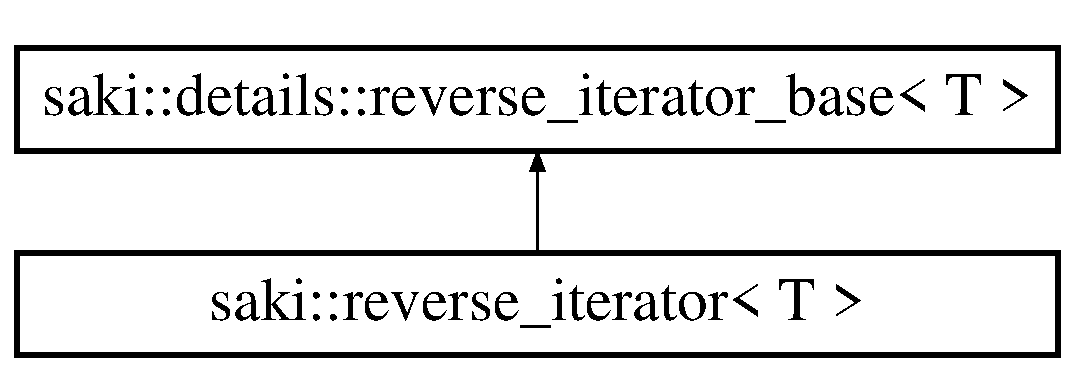
\includegraphics[height=2.000000cm]{classsaki_1_1reverse__iterator}
\end{center}
\end{figure}
\subsection*{公開メンバ関数}
\begin{DoxyCompactItemize}
\item 
constexpr \mbox{\hyperlink{classsaki_1_1reverse__iterator_aed4bbf5a55d71b1f95e2a24d5dc88158}{reverse\+\_\+iterator}} (T pointer)
\end{DoxyCompactItemize}
\subsection*{その他の継承メンバ}


\subsection{詳解}
\subsubsection*{template$<$typename T$>$\newline
class saki\+::reverse\+\_\+iterator$<$ T $>$}

ノーマルなリバースイテレーター 

\subsection{構築子と解体子}
\mbox{\Hypertarget{classsaki_1_1reverse__iterator_aed4bbf5a55d71b1f95e2a24d5dc88158}\label{classsaki_1_1reverse__iterator_aed4bbf5a55d71b1f95e2a24d5dc88158}} 
\index{saki\+::reverse\+\_\+iterator@{saki\+::reverse\+\_\+iterator}!reverse\+\_\+iterator@{reverse\+\_\+iterator}}
\index{reverse\+\_\+iterator@{reverse\+\_\+iterator}!saki\+::reverse\+\_\+iterator@{saki\+::reverse\+\_\+iterator}}
\subsubsection{\texorpdfstring{reverse\+\_\+iterator()}{reverse\_iterator()}}
{\footnotesize\ttfamily template$<$typename T $>$ \\
constexpr \mbox{\hyperlink{classsaki_1_1reverse__iterator}{saki\+::reverse\+\_\+iterator}}$<$ T $>$\+::\mbox{\hyperlink{classsaki_1_1reverse__iterator}{reverse\+\_\+iterator}} (\begin{DoxyParamCaption}\item[{T}]{pointer }\end{DoxyParamCaption})\hspace{0.3cm}{\ttfamily [inline]}, {\ttfamily [explicit]}}



このクラス詳解は次のファイルから抽出されました\+:\begin{DoxyCompactItemize}
\item 
C\+:/\+Users/tokir/\+Documents/\+Git\+Hub/\+Saki\+Cpp\+Library/saki/iterator/reverse/\mbox{\hyperlink{reverse__iterator_8h}{reverse\+\_\+iterator.\+h}}\end{DoxyCompactItemize}

\hypertarget{classsaki_1_1details_1_1reverse__iterator__base}{}\section{saki\+:\+:details\+:\+:reverse\+\_\+iterator\+\_\+base$<$ T $>$ クラステンプレート}
\label{classsaki_1_1details_1_1reverse__iterator__base}\index{saki\+::details\+::reverse\+\_\+iterator\+\_\+base$<$ T $>$@{saki\+::details\+::reverse\+\_\+iterator\+\_\+base$<$ T $>$}}


リバースイテレーターのベースクラス  




{\ttfamily \#include $<$reverse\+\_\+iterator\+\_\+base.\+h$>$}

saki\+:\+:details\+:\+:reverse\+\_\+iterator\+\_\+base$<$ T $>$ の継承関係図\begin{figure}[H]
\begin{center}
\leavevmode
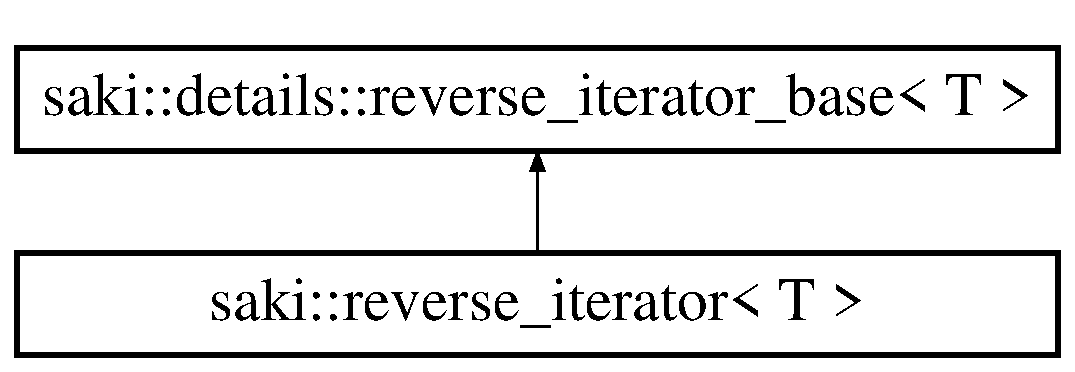
\includegraphics[height=2.000000cm]{classsaki_1_1details_1_1reverse__iterator__base}
\end{center}
\end{figure}
\subsection*{公開メンバ関数}
\begin{DoxyCompactItemize}
\item 
constexpr \mbox{\hyperlink{classsaki_1_1details_1_1reverse__iterator__base_accf1bbae68adfab1bf6e88927e3bc453}{reverse\+\_\+iterator\+\_\+base}} (T \+\_\+itr)
\item 
constexpr T\+::reference \mbox{\hyperlink{classsaki_1_1details_1_1reverse__iterator__base_a7f5228433a205d730e987452ff6e8800}{operator$\ast$}} () const
\begin{DoxyCompactList}\small\item\em 間接参照演算子 \end{DoxyCompactList}\item 
constexpr T\+::pointer \mbox{\hyperlink{classsaki_1_1details_1_1reverse__iterator__base_a15f86c8e2c5830b9b3eaf92cee6fb578}{operator-\/$>$}} () const
\begin{DoxyCompactList}\small\item\em アロー演算子 \end{DoxyCompactList}\item 
constexpr \mbox{\hyperlink{classsaki_1_1details_1_1reverse__iterator__base}{saki\+::details\+::reverse\+\_\+iterator\+\_\+base}}$<$ T $>$ \& \mbox{\hyperlink{classsaki_1_1details_1_1reverse__iterator__base_a6e8e3c069dea1df9a848c95ffe60acbb}{operator++}} ()
\begin{DoxyCompactList}\small\item\em ++演算子(前置) \end{DoxyCompactList}\item 
constexpr \mbox{\hyperlink{classsaki_1_1details_1_1reverse__iterator__base}{saki\+::details\+::reverse\+\_\+iterator\+\_\+base}}$<$ T $>$ \mbox{\hyperlink{classsaki_1_1details_1_1reverse__iterator__base_a7cd2bc5d74938f93c2b07e059068f830}{operator++}} (int)
\begin{DoxyCompactList}\small\item\em ++演算子(後置) \end{DoxyCompactList}\item 
constexpr \mbox{\hyperlink{classsaki_1_1details_1_1reverse__iterator__base}{saki\+::details\+::reverse\+\_\+iterator\+\_\+base}}$<$ T $>$ \& \mbox{\hyperlink{classsaki_1_1details_1_1reverse__iterator__base_aea4bcf44b41d1d5cdb37a630ed9a2e4e}{operator-\/-\/}} ()
\begin{DoxyCompactList}\small\item\em --演算子(前置) \end{DoxyCompactList}\item 
constexpr \mbox{\hyperlink{classsaki_1_1details_1_1reverse__iterator__base}{saki\+::details\+::reverse\+\_\+iterator\+\_\+base}}$<$ T $>$ \mbox{\hyperlink{classsaki_1_1details_1_1reverse__iterator__base_a244654b13c3e164f5382b1216fc5be1f}{operator-\/-\/}} (int)
\begin{DoxyCompactList}\small\item\em --演算子(後置) \end{DoxyCompactList}\end{DoxyCompactItemize}
\subsection*{限定公開変数類}
\begin{DoxyCompactItemize}
\item 
T \mbox{\hyperlink{classsaki_1_1details_1_1reverse__iterator__base_a02df09641bd727c19566dca6c219f279}{itr}}
\end{DoxyCompactItemize}
\subsection*{フレンド}
\begin{DoxyCompactItemize}
\item 
{\footnotesize template$<$typename TT $>$ }\\constexpr bool \mbox{\hyperlink{classsaki_1_1details_1_1reverse__iterator__base_ad8dd5df90aef93e3b60ea87f584a6acf}{operator==}} (const \mbox{\hyperlink{classsaki_1_1details_1_1reverse__iterator__base}{reverse\+\_\+iterator\+\_\+base}}$<$ TT $>$ \&itr1, const \mbox{\hyperlink{classsaki_1_1details_1_1reverse__iterator__base}{reverse\+\_\+iterator\+\_\+base}}$<$ TT $>$ \&itr2)
\item 
{\footnotesize template$<$typename TT $>$ }\\constexpr bool \mbox{\hyperlink{classsaki_1_1details_1_1reverse__iterator__base_a4f19034a62d0d61440f64e39642e2cc6}{operator!=}} (const \mbox{\hyperlink{classsaki_1_1details_1_1reverse__iterator__base}{reverse\+\_\+iterator\+\_\+base}}$<$ TT $>$ \&itr1, const \mbox{\hyperlink{classsaki_1_1details_1_1reverse__iterator__base}{reverse\+\_\+iterator\+\_\+base}}$<$ TT $>$ \&itr2)
\end{DoxyCompactItemize}


\subsection{詳解}
\subsubsection*{template$<$typename T$>$\newline
class saki\+::details\+::reverse\+\_\+iterator\+\_\+base$<$ T $>$}

リバースイテレーターのベースクラス 

\subsection{構築子と解体子}
\mbox{\Hypertarget{classsaki_1_1details_1_1reverse__iterator__base_accf1bbae68adfab1bf6e88927e3bc453}\label{classsaki_1_1details_1_1reverse__iterator__base_accf1bbae68adfab1bf6e88927e3bc453}} 
\index{saki\+::details\+::reverse\+\_\+iterator\+\_\+base@{saki\+::details\+::reverse\+\_\+iterator\+\_\+base}!reverse\+\_\+iterator\+\_\+base@{reverse\+\_\+iterator\+\_\+base}}
\index{reverse\+\_\+iterator\+\_\+base@{reverse\+\_\+iterator\+\_\+base}!saki\+::details\+::reverse\+\_\+iterator\+\_\+base@{saki\+::details\+::reverse\+\_\+iterator\+\_\+base}}
\subsubsection{\texorpdfstring{reverse\+\_\+iterator\+\_\+base()}{reverse\_iterator\_base()}}
{\footnotesize\ttfamily template$<$typename T$>$ \\
constexpr \mbox{\hyperlink{classsaki_1_1details_1_1reverse__iterator__base}{saki\+::details\+::reverse\+\_\+iterator\+\_\+base}}$<$ T $>$\+::\mbox{\hyperlink{classsaki_1_1details_1_1reverse__iterator__base}{reverse\+\_\+iterator\+\_\+base}} (\begin{DoxyParamCaption}\item[{T}]{\+\_\+itr }\end{DoxyParamCaption})\hspace{0.3cm}{\ttfamily [inline]}, {\ttfamily [explicit]}}



\subsection{関数詳解}
\mbox{\Hypertarget{classsaki_1_1details_1_1reverse__iterator__base_a7f5228433a205d730e987452ff6e8800}\label{classsaki_1_1details_1_1reverse__iterator__base_a7f5228433a205d730e987452ff6e8800}} 
\index{saki\+::details\+::reverse\+\_\+iterator\+\_\+base@{saki\+::details\+::reverse\+\_\+iterator\+\_\+base}!operator$\ast$@{operator$\ast$}}
\index{operator$\ast$@{operator$\ast$}!saki\+::details\+::reverse\+\_\+iterator\+\_\+base@{saki\+::details\+::reverse\+\_\+iterator\+\_\+base}}
\subsubsection{\texorpdfstring{operator$\ast$()}{operator*()}}
{\footnotesize\ttfamily template$<$typename T$>$ \\
constexpr T\+::reference \mbox{\hyperlink{classsaki_1_1details_1_1reverse__iterator__base}{saki\+::details\+::reverse\+\_\+iterator\+\_\+base}}$<$ T $>$\+::operator$\ast$ (\begin{DoxyParamCaption}{ }\end{DoxyParamCaption}) const\hspace{0.3cm}{\ttfamily [inline]}}



間接参照演算子 

\mbox{\Hypertarget{classsaki_1_1details_1_1reverse__iterator__base_a6e8e3c069dea1df9a848c95ffe60acbb}\label{classsaki_1_1details_1_1reverse__iterator__base_a6e8e3c069dea1df9a848c95ffe60acbb}} 
\index{saki\+::details\+::reverse\+\_\+iterator\+\_\+base@{saki\+::details\+::reverse\+\_\+iterator\+\_\+base}!operator++@{operator++}}
\index{operator++@{operator++}!saki\+::details\+::reverse\+\_\+iterator\+\_\+base@{saki\+::details\+::reverse\+\_\+iterator\+\_\+base}}
\subsubsection{\texorpdfstring{operator++()}{operator++()}\hspace{0.1cm}{\footnotesize\ttfamily [1/2]}}
{\footnotesize\ttfamily template$<$typename T$>$ \\
constexpr \mbox{\hyperlink{classsaki_1_1details_1_1reverse__iterator__base}{saki\+::details\+::reverse\+\_\+iterator\+\_\+base}}$<$T$>$\& \mbox{\hyperlink{classsaki_1_1details_1_1reverse__iterator__base}{saki\+::details\+::reverse\+\_\+iterator\+\_\+base}}$<$ T $>$\+::operator++ (\begin{DoxyParamCaption}{ }\end{DoxyParamCaption})\hspace{0.3cm}{\ttfamily [inline]}}



++演算子(前置) 

\mbox{\Hypertarget{classsaki_1_1details_1_1reverse__iterator__base_a7cd2bc5d74938f93c2b07e059068f830}\label{classsaki_1_1details_1_1reverse__iterator__base_a7cd2bc5d74938f93c2b07e059068f830}} 
\index{saki\+::details\+::reverse\+\_\+iterator\+\_\+base@{saki\+::details\+::reverse\+\_\+iterator\+\_\+base}!operator++@{operator++}}
\index{operator++@{operator++}!saki\+::details\+::reverse\+\_\+iterator\+\_\+base@{saki\+::details\+::reverse\+\_\+iterator\+\_\+base}}
\subsubsection{\texorpdfstring{operator++()}{operator++()}\hspace{0.1cm}{\footnotesize\ttfamily [2/2]}}
{\footnotesize\ttfamily template$<$typename T$>$ \\
constexpr \mbox{\hyperlink{classsaki_1_1details_1_1reverse__iterator__base}{saki\+::details\+::reverse\+\_\+iterator\+\_\+base}}$<$T$>$ \mbox{\hyperlink{classsaki_1_1details_1_1reverse__iterator__base}{saki\+::details\+::reverse\+\_\+iterator\+\_\+base}}$<$ T $>$\+::operator++ (\begin{DoxyParamCaption}\item[{int}]{ }\end{DoxyParamCaption})\hspace{0.3cm}{\ttfamily [inline]}}



++演算子(後置) 

\mbox{\Hypertarget{classsaki_1_1details_1_1reverse__iterator__base_aea4bcf44b41d1d5cdb37a630ed9a2e4e}\label{classsaki_1_1details_1_1reverse__iterator__base_aea4bcf44b41d1d5cdb37a630ed9a2e4e}} 
\index{saki\+::details\+::reverse\+\_\+iterator\+\_\+base@{saki\+::details\+::reverse\+\_\+iterator\+\_\+base}!operator-\/-\/@{operator-\/-\/}}
\index{operator-\/-\/@{operator-\/-\/}!saki\+::details\+::reverse\+\_\+iterator\+\_\+base@{saki\+::details\+::reverse\+\_\+iterator\+\_\+base}}
\subsubsection{\texorpdfstring{operator-\/-\/()}{operator--()}\hspace{0.1cm}{\footnotesize\ttfamily [1/2]}}
{\footnotesize\ttfamily template$<$typename T$>$ \\
constexpr \mbox{\hyperlink{classsaki_1_1details_1_1reverse__iterator__base}{saki\+::details\+::reverse\+\_\+iterator\+\_\+base}}$<$T$>$\& \mbox{\hyperlink{classsaki_1_1details_1_1reverse__iterator__base}{saki\+::details\+::reverse\+\_\+iterator\+\_\+base}}$<$ T $>$\+::operator-\/-\/ (\begin{DoxyParamCaption}{ }\end{DoxyParamCaption})\hspace{0.3cm}{\ttfamily [inline]}}



--演算子(前置) 

\mbox{\Hypertarget{classsaki_1_1details_1_1reverse__iterator__base_a244654b13c3e164f5382b1216fc5be1f}\label{classsaki_1_1details_1_1reverse__iterator__base_a244654b13c3e164f5382b1216fc5be1f}} 
\index{saki\+::details\+::reverse\+\_\+iterator\+\_\+base@{saki\+::details\+::reverse\+\_\+iterator\+\_\+base}!operator-\/-\/@{operator-\/-\/}}
\index{operator-\/-\/@{operator-\/-\/}!saki\+::details\+::reverse\+\_\+iterator\+\_\+base@{saki\+::details\+::reverse\+\_\+iterator\+\_\+base}}
\subsubsection{\texorpdfstring{operator-\/-\/()}{operator--()}\hspace{0.1cm}{\footnotesize\ttfamily [2/2]}}
{\footnotesize\ttfamily template$<$typename T$>$ \\
constexpr \mbox{\hyperlink{classsaki_1_1details_1_1reverse__iterator__base}{saki\+::details\+::reverse\+\_\+iterator\+\_\+base}}$<$T$>$ \mbox{\hyperlink{classsaki_1_1details_1_1reverse__iterator__base}{saki\+::details\+::reverse\+\_\+iterator\+\_\+base}}$<$ T $>$\+::operator-\/-\/ (\begin{DoxyParamCaption}\item[{int}]{ }\end{DoxyParamCaption})\hspace{0.3cm}{\ttfamily [inline]}}



--演算子(後置) 

\mbox{\Hypertarget{classsaki_1_1details_1_1reverse__iterator__base_a15f86c8e2c5830b9b3eaf92cee6fb578}\label{classsaki_1_1details_1_1reverse__iterator__base_a15f86c8e2c5830b9b3eaf92cee6fb578}} 
\index{saki\+::details\+::reverse\+\_\+iterator\+\_\+base@{saki\+::details\+::reverse\+\_\+iterator\+\_\+base}!operator-\/$>$@{operator-\/$>$}}
\index{operator-\/$>$@{operator-\/$>$}!saki\+::details\+::reverse\+\_\+iterator\+\_\+base@{saki\+::details\+::reverse\+\_\+iterator\+\_\+base}}
\subsubsection{\texorpdfstring{operator-\/$>$()}{operator->()}}
{\footnotesize\ttfamily template$<$typename T$>$ \\
constexpr T\+::pointer \mbox{\hyperlink{classsaki_1_1details_1_1reverse__iterator__base}{saki\+::details\+::reverse\+\_\+iterator\+\_\+base}}$<$ T $>$\+::operator-\/$>$ (\begin{DoxyParamCaption}{ }\end{DoxyParamCaption}) const\hspace{0.3cm}{\ttfamily [inline]}}



アロー演算子 



\subsection{フレンドと関連関数の詳解}
\mbox{\Hypertarget{classsaki_1_1details_1_1reverse__iterator__base_a4f19034a62d0d61440f64e39642e2cc6}\label{classsaki_1_1details_1_1reverse__iterator__base_a4f19034a62d0d61440f64e39642e2cc6}} 
\index{saki\+::details\+::reverse\+\_\+iterator\+\_\+base@{saki\+::details\+::reverse\+\_\+iterator\+\_\+base}!operator"!=@{operator"!=}}
\index{operator"!=@{operator"!=}!saki\+::details\+::reverse\+\_\+iterator\+\_\+base@{saki\+::details\+::reverse\+\_\+iterator\+\_\+base}}
\subsubsection{\texorpdfstring{operator"!=}{operator!=}}
{\footnotesize\ttfamily template$<$typename T$>$ \\
template$<$typename TT $>$ \\
constexpr bool operator!= (\begin{DoxyParamCaption}\item[{const \mbox{\hyperlink{classsaki_1_1details_1_1reverse__iterator__base}{reverse\+\_\+iterator\+\_\+base}}$<$ TT $>$ \&}]{itr1,  }\item[{const \mbox{\hyperlink{classsaki_1_1details_1_1reverse__iterator__base}{reverse\+\_\+iterator\+\_\+base}}$<$ TT $>$ \&}]{itr2 }\end{DoxyParamCaption})\hspace{0.3cm}{\ttfamily [friend]}}

\mbox{\Hypertarget{classsaki_1_1details_1_1reverse__iterator__base_ad8dd5df90aef93e3b60ea87f584a6acf}\label{classsaki_1_1details_1_1reverse__iterator__base_ad8dd5df90aef93e3b60ea87f584a6acf}} 
\index{saki\+::details\+::reverse\+\_\+iterator\+\_\+base@{saki\+::details\+::reverse\+\_\+iterator\+\_\+base}!operator==@{operator==}}
\index{operator==@{operator==}!saki\+::details\+::reverse\+\_\+iterator\+\_\+base@{saki\+::details\+::reverse\+\_\+iterator\+\_\+base}}
\subsubsection{\texorpdfstring{operator==}{operator==}}
{\footnotesize\ttfamily template$<$typename T$>$ \\
template$<$typename TT $>$ \\
constexpr bool operator== (\begin{DoxyParamCaption}\item[{const \mbox{\hyperlink{classsaki_1_1details_1_1reverse__iterator__base}{reverse\+\_\+iterator\+\_\+base}}$<$ TT $>$ \&}]{itr1,  }\item[{const \mbox{\hyperlink{classsaki_1_1details_1_1reverse__iterator__base}{reverse\+\_\+iterator\+\_\+base}}$<$ TT $>$ \&}]{itr2 }\end{DoxyParamCaption})\hspace{0.3cm}{\ttfamily [friend]}}



\subsection{メンバ詳解}
\mbox{\Hypertarget{classsaki_1_1details_1_1reverse__iterator__base_a02df09641bd727c19566dca6c219f279}\label{classsaki_1_1details_1_1reverse__iterator__base_a02df09641bd727c19566dca6c219f279}} 
\index{saki\+::details\+::reverse\+\_\+iterator\+\_\+base@{saki\+::details\+::reverse\+\_\+iterator\+\_\+base}!itr@{itr}}
\index{itr@{itr}!saki\+::details\+::reverse\+\_\+iterator\+\_\+base@{saki\+::details\+::reverse\+\_\+iterator\+\_\+base}}
\subsubsection{\texorpdfstring{itr}{itr}}
{\footnotesize\ttfamily template$<$typename T$>$ \\
T \mbox{\hyperlink{classsaki_1_1details_1_1reverse__iterator__base}{saki\+::details\+::reverse\+\_\+iterator\+\_\+base}}$<$ T $>$\+::itr\hspace{0.3cm}{\ttfamily [protected]}}



このクラス詳解は次のファイルから抽出されました\+:\begin{DoxyCompactItemize}
\item 
C\+:/\+Users/tokir/\+Documents/\+Git\+Hub/\+Saki\+Cpp\+Library/saki/iterator/reverse/details/\mbox{\hyperlink{reverse__iterator__base_8h}{reverse\+\_\+iterator\+\_\+base.\+h}}\end{DoxyCompactItemize}

\hypertarget{classsaki_1_1singleton}{}\section{saki\+:\+:singleton$<$ T $>$ クラステンプレート}
\label{classsaki_1_1singleton}\index{saki\+::singleton$<$ T $>$@{saki\+::singleton$<$ T $>$}}


継承するとシングルトンクラスになる  




{\ttfamily \#include $<$singleton.\+h$>$}

\subsection*{公開メンバ関数}
\begin{DoxyCompactItemize}
\item 
virtual \mbox{\hyperlink{classsaki_1_1singleton_a7e18a317dec7a4658f6d3376f2dd3ebd}{$\sim$singleton}} ()
\end{DoxyCompactItemize}
\subsection*{静的公開メンバ関数}
\begin{DoxyCompactItemize}
\item 
static std\+::unique\+\_\+ptr$<$ T $>$ \& \mbox{\hyperlink{classsaki_1_1singleton_a17071f9daca33c8dd4287dffc49457ec}{getinstance}} ()
\begin{DoxyCompactList}\small\item\em インスタンスを取得 \end{DoxyCompactList}\end{DoxyCompactItemize}
\subsection*{限定公開メンバ関数}
\begin{DoxyCompactItemize}
\item 
\mbox{\hyperlink{classsaki_1_1singleton_a511f5d5e51fdac173fa0dbea858f5ee0}{singleton}} ()
\end{DoxyCompactItemize}


\subsection{詳解}
\subsubsection*{template$<$typename T$>$\newline
class saki\+::singleton$<$ T $>$}

継承するとシングルトンクラスになる 

\subsection{構築子と解体子}
\mbox{\Hypertarget{classsaki_1_1singleton_a7e18a317dec7a4658f6d3376f2dd3ebd}\label{classsaki_1_1singleton_a7e18a317dec7a4658f6d3376f2dd3ebd}} 
\index{saki\+::singleton@{saki\+::singleton}!````~singleton@{$\sim$singleton}}
\index{````~singleton@{$\sim$singleton}!saki\+::singleton@{saki\+::singleton}}
\subsubsection{\texorpdfstring{$\sim$singleton()}{~singleton()}}
{\footnotesize\ttfamily template$<$typename T $>$ \\
virtual \mbox{\hyperlink{classsaki_1_1singleton}{saki\+::singleton}}$<$ T $>$\+::$\sim$\mbox{\hyperlink{classsaki_1_1singleton}{singleton}} (\begin{DoxyParamCaption}{ }\end{DoxyParamCaption})\hspace{0.3cm}{\ttfamily [inline]}, {\ttfamily [virtual]}}

\mbox{\Hypertarget{classsaki_1_1singleton_a511f5d5e51fdac173fa0dbea858f5ee0}\label{classsaki_1_1singleton_a511f5d5e51fdac173fa0dbea858f5ee0}} 
\index{saki\+::singleton@{saki\+::singleton}!singleton@{singleton}}
\index{singleton@{singleton}!saki\+::singleton@{saki\+::singleton}}
\subsubsection{\texorpdfstring{singleton()}{singleton()}}
{\footnotesize\ttfamily template$<$typename T $>$ \\
\mbox{\hyperlink{classsaki_1_1singleton}{saki\+::singleton}}$<$ T $>$\+::\mbox{\hyperlink{classsaki_1_1singleton}{singleton}} (\begin{DoxyParamCaption}{ }\end{DoxyParamCaption})\hspace{0.3cm}{\ttfamily [inline]}, {\ttfamily [protected]}}



\subsection{関数詳解}
\mbox{\Hypertarget{classsaki_1_1singleton_a17071f9daca33c8dd4287dffc49457ec}\label{classsaki_1_1singleton_a17071f9daca33c8dd4287dffc49457ec}} 
\index{saki\+::singleton@{saki\+::singleton}!getinstance@{getinstance}}
\index{getinstance@{getinstance}!saki\+::singleton@{saki\+::singleton}}
\subsubsection{\texorpdfstring{getinstance()}{getinstance()}}
{\footnotesize\ttfamily template$<$typename T $>$ \\
static std\+::unique\+\_\+ptr$<$T$>$\& \mbox{\hyperlink{classsaki_1_1singleton}{saki\+::singleton}}$<$ T $>$\+::getinstance (\begin{DoxyParamCaption}{ }\end{DoxyParamCaption})\hspace{0.3cm}{\ttfamily [inline]}, {\ttfamily [static]}}



インスタンスを取得 

\begin{DoxyReturn}{戻り値}
std\+::unique\+\_\+ptr$<$\+T$>$ インスタンスを返す 
\end{DoxyReturn}


このクラス詳解は次のファイルから抽出されました\+:\begin{DoxyCompactItemize}
\item 
C\+:/\+Users/tokir/\+Documents/\+Git\+Hub/\+Saki\+Cpp\+Library/saki/singleton/\mbox{\hyperlink{singleton_2singleton_8h}{singleton.\+h}}\end{DoxyCompactItemize}

\hypertarget{classsaki_1_1string__base}{}\section{saki\+:\+:string\+\_\+base$<$ T, N $>$ クラステンプレート}
\label{classsaki_1_1string__base}\index{saki\+::string\+\_\+base$<$ T, N $>$@{saki\+::string\+\_\+base$<$ T, N $>$}}


コンパイル時固定長string\+\_\+baseクラス  




{\ttfamily \#include $<$string.\+h$>$}

\subsection*{公開メンバ関数}
\begin{DoxyCompactItemize}
\item 
constexpr \mbox{\hyperlink{classsaki_1_1string__base_a5301a26e787034be1365a23964a267fd}{string\+\_\+base}} ()
\item 
constexpr \mbox{\hyperlink{classsaki_1_1string__base_a72a95e9a65c0e1e4bcbd47fca9c78281}{string\+\_\+base}} (const \mbox{\hyperlink{classsaki_1_1array}{saki\+::array}}$<$ T, N $>$ \&arr)
\item 
constexpr T \& \mbox{\hyperlink{classsaki_1_1string__base_aca7367871a2c8e1722032240f4fa42fa}{operator\mbox{[}$\,$\mbox{]}}} (size\+\_\+t index)
\item 
constexpr const T \& \mbox{\hyperlink{classsaki_1_1string__base_abfd90384f8529e8ac5cecb910000ac3b}{operator\mbox{[}$\,$\mbox{]}}} (size\+\_\+t index) const
\end{DoxyCompactItemize}


\subsection{詳解}
\subsubsection*{template$<$typename T, size\+\_\+t N$>$\newline
class saki\+::string\+\_\+base$<$ T, N $>$}

コンパイル時固定長string\+\_\+baseクラス 

\subsection{構築子と解体子}
\mbox{\Hypertarget{classsaki_1_1string__base_a5301a26e787034be1365a23964a267fd}\label{classsaki_1_1string__base_a5301a26e787034be1365a23964a267fd}} 
\index{saki\+::string\+\_\+base@{saki\+::string\+\_\+base}!string\+\_\+base@{string\+\_\+base}}
\index{string\+\_\+base@{string\+\_\+base}!saki\+::string\+\_\+base@{saki\+::string\+\_\+base}}
\subsubsection{\texorpdfstring{string\+\_\+base()}{string\_base()}\hspace{0.1cm}{\footnotesize\ttfamily [1/2]}}
{\footnotesize\ttfamily template$<$typename T , size\+\_\+t N$>$ \\
constexpr \mbox{\hyperlink{classsaki_1_1string__base}{saki\+::string\+\_\+base}}$<$ T, N $>$\+::\mbox{\hyperlink{classsaki_1_1string__base}{string\+\_\+base}} (\begin{DoxyParamCaption}{ }\end{DoxyParamCaption})\hspace{0.3cm}{\ttfamily [inline]}}

\mbox{\Hypertarget{classsaki_1_1string__base_a72a95e9a65c0e1e4bcbd47fca9c78281}\label{classsaki_1_1string__base_a72a95e9a65c0e1e4bcbd47fca9c78281}} 
\index{saki\+::string\+\_\+base@{saki\+::string\+\_\+base}!string\+\_\+base@{string\+\_\+base}}
\index{string\+\_\+base@{string\+\_\+base}!saki\+::string\+\_\+base@{saki\+::string\+\_\+base}}
\subsubsection{\texorpdfstring{string\+\_\+base()}{string\_base()}\hspace{0.1cm}{\footnotesize\ttfamily [2/2]}}
{\footnotesize\ttfamily template$<$typename T , size\+\_\+t N$>$ \\
constexpr \mbox{\hyperlink{classsaki_1_1string__base}{saki\+::string\+\_\+base}}$<$ T, N $>$\+::\mbox{\hyperlink{classsaki_1_1string__base}{string\+\_\+base}} (\begin{DoxyParamCaption}\item[{const \mbox{\hyperlink{classsaki_1_1array}{saki\+::array}}$<$ T, N $>$ \&}]{arr }\end{DoxyParamCaption})\hspace{0.3cm}{\ttfamily [inline]}}



\subsection{関数詳解}
\mbox{\Hypertarget{classsaki_1_1string__base_aca7367871a2c8e1722032240f4fa42fa}\label{classsaki_1_1string__base_aca7367871a2c8e1722032240f4fa42fa}} 
\index{saki\+::string\+\_\+base@{saki\+::string\+\_\+base}!operator\mbox{[}\mbox{]}@{operator[]}}
\index{operator\mbox{[}\mbox{]}@{operator[]}!saki\+::string\+\_\+base@{saki\+::string\+\_\+base}}
\subsubsection{\texorpdfstring{operator[]()}{operator[]()}\hspace{0.1cm}{\footnotesize\ttfamily [1/2]}}
{\footnotesize\ttfamily template$<$typename T , size\+\_\+t N$>$ \\
constexpr T\& \mbox{\hyperlink{classsaki_1_1string__base}{saki\+::string\+\_\+base}}$<$ T, N $>$\+::operator\mbox{[}$\,$\mbox{]} (\begin{DoxyParamCaption}\item[{size\+\_\+t}]{index }\end{DoxyParamCaption})\hspace{0.3cm}{\ttfamily [inline]}}

\mbox{\Hypertarget{classsaki_1_1string__base_abfd90384f8529e8ac5cecb910000ac3b}\label{classsaki_1_1string__base_abfd90384f8529e8ac5cecb910000ac3b}} 
\index{saki\+::string\+\_\+base@{saki\+::string\+\_\+base}!operator\mbox{[}\mbox{]}@{operator[]}}
\index{operator\mbox{[}\mbox{]}@{operator[]}!saki\+::string\+\_\+base@{saki\+::string\+\_\+base}}
\subsubsection{\texorpdfstring{operator[]()}{operator[]()}\hspace{0.1cm}{\footnotesize\ttfamily [2/2]}}
{\footnotesize\ttfamily template$<$typename T , size\+\_\+t N$>$ \\
constexpr const T\& \mbox{\hyperlink{classsaki_1_1string__base}{saki\+::string\+\_\+base}}$<$ T, N $>$\+::operator\mbox{[}$\,$\mbox{]} (\begin{DoxyParamCaption}\item[{size\+\_\+t}]{index }\end{DoxyParamCaption}) const\hspace{0.3cm}{\ttfamily [inline]}}



このクラス詳解は次のファイルから抽出されました\+:\begin{DoxyCompactItemize}
\item 
C\+:/\+Users/tokir/\+Documents/\+Git\+Hub/\+Saki\+Cpp\+Library/saki/string/\mbox{\hyperlink{string_2string_8h}{string.\+h}}\end{DoxyCompactItemize}

\hypertarget{structsaki_1_1subtraction}{}\section{saki\+:\+:subtraction 構造体}
\label{structsaki_1_1subtraction}\index{saki\+::subtraction@{saki\+::subtraction}}


引き算のconstexpr対応した関数オブジェクト  




{\ttfamily \#include $<$subtraction.\+hpp$>$}

\subsection*{公開メンバ関数}
\begin{DoxyCompactItemize}
\item 
{\footnotesize template$<$typename T1 , typename T2 $>$ }\\constexpr auto \mbox{\hyperlink{structsaki_1_1subtraction_a5de4626c125df92e70848fcac27eef74}{operator()}} (const T1 \&t1, const T2 \&t2) const -\/$>$ decltype(t1 -\/ t2)
\end{DoxyCompactItemize}


\subsection{詳解}
引き算のconstexpr対応した関数オブジェクト 

\subsection{関数詳解}
\mbox{\Hypertarget{structsaki_1_1subtraction_a5de4626c125df92e70848fcac27eef74}\label{structsaki_1_1subtraction_a5de4626c125df92e70848fcac27eef74}} 
\index{saki\+::subtraction@{saki\+::subtraction}!operator()@{operator()}}
\index{operator()@{operator()}!saki\+::subtraction@{saki\+::subtraction}}
\subsubsection{\texorpdfstring{operator()()}{operator()()}}
{\footnotesize\ttfamily template$<$typename T1 , typename T2 $>$ \\
constexpr auto saki\+::subtraction\+::operator() (\begin{DoxyParamCaption}\item[{const T1 \&}]{t1,  }\item[{const T2 \&}]{t2 }\end{DoxyParamCaption}) const -\/$>$ decltype(t1 -\/ t2)
	\hspace{0.3cm}{\ttfamily [inline]}}



この構造体詳解は次のファイルから抽出されました\+:\begin{DoxyCompactItemize}
\item 
C\+:/\+Users/tokir/\+Documents/\+Git\+Hub/\+Saki\+Cpp\+Library/saki/function\+\_\+object/\mbox{\hyperlink{subtraction_8hpp}{subtraction.\+hpp}}\end{DoxyCompactItemize}

\hypertarget{classsaki_1_1transform}{}\section{saki\+:\+:transform$<$ T $>$ クラステンプレート}
\label{classsaki_1_1transform}\index{saki\+::transform$<$ T $>$@{saki\+::transform$<$ T $>$}}


transformクラス  




{\ttfamily \#include $<$transform\+\_\+operator.\+h$>$}

\subsection*{公開メンバ関数}
\begin{DoxyCompactItemize}
\item 
constexpr \mbox{\hyperlink{classsaki_1_1transform_a6d3d745d729424d11a67514dcbedfc4b}{transform}} ()
\begin{DoxyCompactList}\small\item\em 引数なしコンストラクタ \end{DoxyCompactList}\item 
constexpr \mbox{\hyperlink{classsaki_1_1transform_ae508c65cf86017bc6deae19eda294dbf}{transform}} (const \mbox{\hyperlink{classsaki_1_1vector3}{saki\+::vector3}}$<$ T $>$ \&pos, const \mbox{\hyperlink{classsaki_1_1vector3}{saki\+::vector3}}$<$ T $>$ rot, const \mbox{\hyperlink{classsaki_1_1vector3}{saki\+::vector3}}$<$ T $>$sca)
\begin{DoxyCompactList}\small\item\em 各値を引数にとるコンストラクタ \end{DoxyCompactList}\item 
\mbox{\hyperlink{classsaki_1_1transform_a973773964975d30d4f4a114ebb94d5ef}{transform}} (const \mbox{\hyperlink{classsaki_1_1transform}{transform}}$<$ T $>$ \&)=default
\item 
\mbox{\hyperlink{classsaki_1_1transform}{transform}}$<$ T $>$ \& \mbox{\hyperlink{classsaki_1_1transform_a02ae1743b6a54bc004b69b5b9ec3e574}{operator=}} (const \mbox{\hyperlink{classsaki_1_1transform}{transform}}$<$ T $>$ \&)=default
\item 
\mbox{\hyperlink{classsaki_1_1transform_a570e4f075582d4c50376f1170bce7af2}{transform}} (\mbox{\hyperlink{classsaki_1_1transform}{transform}}$<$ T $>$ \&\&)=default
\item 
\mbox{\hyperlink{classsaki_1_1transform}{transform}}$<$ T $>$ \& \mbox{\hyperlink{classsaki_1_1transform_aa43de25eaecdc6d713f83998247e9736}{operator=}} (\mbox{\hyperlink{classsaki_1_1transform}{transform}}$<$ T $>$ \&\&)=default
\item 
constexpr void \mbox{\hyperlink{classsaki_1_1transform_a24a42ef2114b77f0e4520b693d677d60}{move}} (const \mbox{\hyperlink{classsaki_1_1vector3}{saki\+::vector3}}$<$ T $>$ \&pos)
\begin{DoxyCompactList}\small\item\em 移動 \end{DoxyCompactList}\item 
constexpr void \mbox{\hyperlink{classsaki_1_1transform_aad46d5a8b608aa9d94fd29a1fe4d5609}{move}} (const T \&x, const T \&y, const T \&z)
\begin{DoxyCompactList}\small\item\em 移動 \end{DoxyCompactList}\item 
constexpr void \mbox{\hyperlink{classsaki_1_1transform_a34a7facf52587a38a40a7ff6643568cf}{rotate}} (const \mbox{\hyperlink{classsaki_1_1vector3}{saki\+::vector3}}$<$ T $>$ \&rot)
\begin{DoxyCompactList}\small\item\em 回転 \end{DoxyCompactList}\item 
constexpr void \mbox{\hyperlink{classsaki_1_1transform_a00065f2da91bca7ac0aff6efd46ac2ae}{rotate}} (const T \&x, const T \&y, const T \&z)
\begin{DoxyCompactList}\small\item\em 回転 \end{DoxyCompactList}\item 
constexpr void \mbox{\hyperlink{classsaki_1_1transform_acb1e4cc039b689a97ed4098f566c7907}{expantion}} (const \mbox{\hyperlink{classsaki_1_1vector3}{saki\+::vector3}}$<$ T $>$ \&sca)
\begin{DoxyCompactList}\small\item\em 拡大 \end{DoxyCompactList}\item 
constexpr void \mbox{\hyperlink{classsaki_1_1transform_ab6c97d4f30cc45b1dc1d200ce7a0c483}{expantion}} (const T \&x, const T \&y, const T \&z)
\begin{DoxyCompactList}\small\item\em 拡大 \end{DoxyCompactList}\item 
constexpr auto \mbox{\hyperlink{classsaki_1_1transform_a6c1489a48121fc89bf7238327dd2a1c4}{get\+\_\+pos}} () const
\begin{DoxyCompactList}\small\item\em 位置のゲッタ \end{DoxyCompactList}\item 
constexpr void \mbox{\hyperlink{classsaki_1_1transform_a11a56e02fe536c08b55655d70548876f}{set\+\_\+pos}} (const \mbox{\hyperlink{classsaki_1_1vector3}{saki\+::vector3}}$<$ T $>$ \&pos)
\begin{DoxyCompactList}\small\item\em 位置のセッタ \end{DoxyCompactList}\item 
constexpr auto \mbox{\hyperlink{classsaki_1_1transform_ad0b5e29b9f201f3fcb34011a146a89c1}{get\+\_\+rot}} () const
\begin{DoxyCompactList}\small\item\em 回転のゲッタ \end{DoxyCompactList}\item 
constexpr void \mbox{\hyperlink{classsaki_1_1transform_a0920b584e25129a5b0d42dbc296abd55}{set\+\_\+rot}} (const \mbox{\hyperlink{classsaki_1_1vector3}{saki\+::vector3}}$<$ T $>$ \&rot)
\begin{DoxyCompactList}\small\item\em 回転のセッタ \end{DoxyCompactList}\item 
constexpr auto \mbox{\hyperlink{classsaki_1_1transform_a8d7e5a36cc869a8b43ee779d90074279}{get\+\_\+scale}} () const
\begin{DoxyCompactList}\small\item\em 拡縮のゲッタ \end{DoxyCompactList}\item 
constexpr void \mbox{\hyperlink{classsaki_1_1transform_ad1423bce28426ae4b739ccb22bc0fd5d}{set\+\_\+scale}} (const \mbox{\hyperlink{classsaki_1_1vector3}{saki\+::vector3}}$<$ T $>$ \&sca)
\begin{DoxyCompactList}\small\item\em 拡縮のセッタ \end{DoxyCompactList}\item 
{\footnotesize template$<$typename U  = T$>$ }\\constexpr auto \mbox{\hyperlink{classsaki_1_1transform_a6478b00898341e47040560a01f0b9cbc}{operator+=}} (const \mbox{\hyperlink{classsaki_1_1transform}{saki\+::transform}}$<$ U $>$ \&other)
\begin{DoxyCompactList}\small\item\em +=演算子 \end{DoxyCompactList}\item 
{\footnotesize template$<$typename U  = T$>$ }\\constexpr auto \mbox{\hyperlink{classsaki_1_1transform_a4ce71c92d3d4944f6773a021d0bd3234}{operator-\/=}} (const \mbox{\hyperlink{classsaki_1_1transform}{saki\+::transform}}$<$ U $>$ \&other)
\begin{DoxyCompactList}\small\item\em -\/=演算子 \end{DoxyCompactList}\item 
{\footnotesize template$<$typename U  = T$>$ }\\constexpr auto \mbox{\hyperlink{classsaki_1_1transform_a239258a92acd6ad904e8a5dea5cc78cf}{operator$\ast$=}} (const U \&scalar)
\begin{DoxyCompactList}\small\item\em $\ast$=演算子(スカラ) \end{DoxyCompactList}\item 
{\footnotesize template$<$typename U  = T$>$ }\\constexpr auto \mbox{\hyperlink{classsaki_1_1transform_a069699ce700d7a69503c17c78b58646e}{operator/=}} (const U \&scalar)
\begin{DoxyCompactList}\small\item\em /= 演算子(スカラ) \end{DoxyCompactList}\item 
constexpr \mbox{\hyperlink{classsaki_1_1transform}{saki\+::transform}}$<$ T $>$ \mbox{\hyperlink{classsaki_1_1transform_a67d95b1c1a7826256f06b1d1345474b5}{operator+}} () const
\begin{DoxyCompactList}\small\item\em 単項+演算子 \end{DoxyCompactList}\item 
constexpr \mbox{\hyperlink{classsaki_1_1transform}{saki\+::transform}}$<$ T $>$ \mbox{\hyperlink{classsaki_1_1transform_aba069deaa467ec2e4ea548b590084916}{operator-\/}} () const
\begin{DoxyCompactList}\small\item\em 単項-\/演算子 \end{DoxyCompactList}\end{DoxyCompactItemize}


\subsection{詳解}
\subsubsection*{template$<$typename T$>$\newline
class saki\+::transform$<$ T $>$}

transformクラス 

クォータニオンは使用していません 

\subsection{構築子と解体子}
\mbox{\Hypertarget{classsaki_1_1transform_a6d3d745d729424d11a67514dcbedfc4b}\label{classsaki_1_1transform_a6d3d745d729424d11a67514dcbedfc4b}} 
\index{saki\+::transform@{saki\+::transform}!transform@{transform}}
\index{transform@{transform}!saki\+::transform@{saki\+::transform}}
\subsubsection{\texorpdfstring{transform()}{transform()}\hspace{0.1cm}{\footnotesize\ttfamily [1/4]}}
{\footnotesize\ttfamily template$<$typename T$>$ \\
constexpr \mbox{\hyperlink{classsaki_1_1transform}{saki\+::transform}}$<$ T $>$\+::\mbox{\hyperlink{classsaki_1_1transform}{transform}} (\begin{DoxyParamCaption}{ }\end{DoxyParamCaption})\hspace{0.3cm}{\ttfamily [inline]}}



引数なしコンストラクタ 

\mbox{\Hypertarget{classsaki_1_1transform_ae508c65cf86017bc6deae19eda294dbf}\label{classsaki_1_1transform_ae508c65cf86017bc6deae19eda294dbf}} 
\index{saki\+::transform@{saki\+::transform}!transform@{transform}}
\index{transform@{transform}!saki\+::transform@{saki\+::transform}}
\subsubsection{\texorpdfstring{transform()}{transform()}\hspace{0.1cm}{\footnotesize\ttfamily [2/4]}}
{\footnotesize\ttfamily template$<$typename T$>$ \\
constexpr \mbox{\hyperlink{classsaki_1_1transform}{saki\+::transform}}$<$ T $>$\+::\mbox{\hyperlink{classsaki_1_1transform}{transform}} (\begin{DoxyParamCaption}\item[{const \mbox{\hyperlink{classsaki_1_1vector3}{saki\+::vector3}}$<$ T $>$ \&}]{pos,  }\item[{const \mbox{\hyperlink{classsaki_1_1vector3}{saki\+::vector3}}$<$ T $>$}]{rot,  }\item[{const \mbox{\hyperlink{classsaki_1_1vector3}{saki\+::vector3}}$<$ T $>$}]{sca }\end{DoxyParamCaption})\hspace{0.3cm}{\ttfamily [inline]}}



各値を引数にとるコンストラクタ 


\begin{DoxyParams}{引数}
{\em pos} & 位置 \\
\hline
{\em rot} & 回転 \\
\hline
{\em sca} & 拡縮 \\
\hline
\end{DoxyParams}
\mbox{\Hypertarget{classsaki_1_1transform_a973773964975d30d4f4a114ebb94d5ef}\label{classsaki_1_1transform_a973773964975d30d4f4a114ebb94d5ef}} 
\index{saki\+::transform@{saki\+::transform}!transform@{transform}}
\index{transform@{transform}!saki\+::transform@{saki\+::transform}}
\subsubsection{\texorpdfstring{transform()}{transform()}\hspace{0.1cm}{\footnotesize\ttfamily [3/4]}}
{\footnotesize\ttfamily template$<$typename T$>$ \\
\mbox{\hyperlink{classsaki_1_1transform}{saki\+::transform}}$<$ T $>$\+::\mbox{\hyperlink{classsaki_1_1transform}{transform}} (\begin{DoxyParamCaption}\item[{const \mbox{\hyperlink{classsaki_1_1transform}{transform}}$<$ T $>$ \&}]{ }\end{DoxyParamCaption})\hspace{0.3cm}{\ttfamily [default]}}

\mbox{\Hypertarget{classsaki_1_1transform_a570e4f075582d4c50376f1170bce7af2}\label{classsaki_1_1transform_a570e4f075582d4c50376f1170bce7af2}} 
\index{saki\+::transform@{saki\+::transform}!transform@{transform}}
\index{transform@{transform}!saki\+::transform@{saki\+::transform}}
\subsubsection{\texorpdfstring{transform()}{transform()}\hspace{0.1cm}{\footnotesize\ttfamily [4/4]}}
{\footnotesize\ttfamily template$<$typename T$>$ \\
\mbox{\hyperlink{classsaki_1_1transform}{saki\+::transform}}$<$ T $>$\+::\mbox{\hyperlink{classsaki_1_1transform}{transform}} (\begin{DoxyParamCaption}\item[{\mbox{\hyperlink{classsaki_1_1transform}{transform}}$<$ T $>$ \&\&}]{ }\end{DoxyParamCaption})\hspace{0.3cm}{\ttfamily [default]}}



\subsection{関数詳解}
\mbox{\Hypertarget{classsaki_1_1transform_acb1e4cc039b689a97ed4098f566c7907}\label{classsaki_1_1transform_acb1e4cc039b689a97ed4098f566c7907}} 
\index{saki\+::transform@{saki\+::transform}!expantion@{expantion}}
\index{expantion@{expantion}!saki\+::transform@{saki\+::transform}}
\subsubsection{\texorpdfstring{expantion()}{expantion()}\hspace{0.1cm}{\footnotesize\ttfamily [1/2]}}
{\footnotesize\ttfamily template$<$typename T$>$ \\
constexpr void \mbox{\hyperlink{classsaki_1_1transform}{saki\+::transform}}$<$ T $>$\+::expantion (\begin{DoxyParamCaption}\item[{const \mbox{\hyperlink{classsaki_1_1vector3}{saki\+::vector3}}$<$ T $>$ \&}]{sca }\end{DoxyParamCaption})\hspace{0.3cm}{\ttfamily [inline]}}



拡大 


\begin{DoxyParams}{引数}
{\em sca} & 拡大量 \\
\hline
\end{DoxyParams}
\mbox{\Hypertarget{classsaki_1_1transform_ab6c97d4f30cc45b1dc1d200ce7a0c483}\label{classsaki_1_1transform_ab6c97d4f30cc45b1dc1d200ce7a0c483}} 
\index{saki\+::transform@{saki\+::transform}!expantion@{expantion}}
\index{expantion@{expantion}!saki\+::transform@{saki\+::transform}}
\subsubsection{\texorpdfstring{expantion()}{expantion()}\hspace{0.1cm}{\footnotesize\ttfamily [2/2]}}
{\footnotesize\ttfamily template$<$typename T$>$ \\
constexpr void \mbox{\hyperlink{classsaki_1_1transform}{saki\+::transform}}$<$ T $>$\+::expantion (\begin{DoxyParamCaption}\item[{const T \&}]{x,  }\item[{const T \&}]{y,  }\item[{const T \&}]{z }\end{DoxyParamCaption})\hspace{0.3cm}{\ttfamily [inline]}}



拡大 


\begin{DoxyParams}{引数}
{\em x} & 拡大量(x) \\
\hline
{\em y} & 拡大量(y) \\
\hline
{\em z} & 拡大量(z) \\
\hline
\end{DoxyParams}
\mbox{\Hypertarget{classsaki_1_1transform_a6c1489a48121fc89bf7238327dd2a1c4}\label{classsaki_1_1transform_a6c1489a48121fc89bf7238327dd2a1c4}} 
\index{saki\+::transform@{saki\+::transform}!get\+\_\+pos@{get\+\_\+pos}}
\index{get\+\_\+pos@{get\+\_\+pos}!saki\+::transform@{saki\+::transform}}
\subsubsection{\texorpdfstring{get\+\_\+pos()}{get\_pos()}}
{\footnotesize\ttfamily template$<$typename T$>$ \\
constexpr auto \mbox{\hyperlink{classsaki_1_1transform}{saki\+::transform}}$<$ T $>$\+::get\+\_\+pos (\begin{DoxyParamCaption}{ }\end{DoxyParamCaption}) const\hspace{0.3cm}{\ttfamily [inline]}}



位置のゲッタ 

\begin{DoxyReturn}{戻り値}
位置 
\end{DoxyReturn}
\mbox{\Hypertarget{classsaki_1_1transform_ad0b5e29b9f201f3fcb34011a146a89c1}\label{classsaki_1_1transform_ad0b5e29b9f201f3fcb34011a146a89c1}} 
\index{saki\+::transform@{saki\+::transform}!get\+\_\+rot@{get\+\_\+rot}}
\index{get\+\_\+rot@{get\+\_\+rot}!saki\+::transform@{saki\+::transform}}
\subsubsection{\texorpdfstring{get\+\_\+rot()}{get\_rot()}}
{\footnotesize\ttfamily template$<$typename T$>$ \\
constexpr auto \mbox{\hyperlink{classsaki_1_1transform}{saki\+::transform}}$<$ T $>$\+::get\+\_\+rot (\begin{DoxyParamCaption}{ }\end{DoxyParamCaption}) const\hspace{0.3cm}{\ttfamily [inline]}}



回転のゲッタ 

\begin{DoxyReturn}{戻り値}
回転 
\end{DoxyReturn}
\mbox{\Hypertarget{classsaki_1_1transform_a8d7e5a36cc869a8b43ee779d90074279}\label{classsaki_1_1transform_a8d7e5a36cc869a8b43ee779d90074279}} 
\index{saki\+::transform@{saki\+::transform}!get\+\_\+scale@{get\+\_\+scale}}
\index{get\+\_\+scale@{get\+\_\+scale}!saki\+::transform@{saki\+::transform}}
\subsubsection{\texorpdfstring{get\+\_\+scale()}{get\_scale()}}
{\footnotesize\ttfamily template$<$typename T$>$ \\
constexpr auto \mbox{\hyperlink{classsaki_1_1transform}{saki\+::transform}}$<$ T $>$\+::get\+\_\+scale (\begin{DoxyParamCaption}{ }\end{DoxyParamCaption}) const\hspace{0.3cm}{\ttfamily [inline]}}



拡縮のゲッタ 

\begin{DoxyReturn}{戻り値}
拡縮 
\end{DoxyReturn}
\mbox{\Hypertarget{classsaki_1_1transform_a24a42ef2114b77f0e4520b693d677d60}\label{classsaki_1_1transform_a24a42ef2114b77f0e4520b693d677d60}} 
\index{saki\+::transform@{saki\+::transform}!move@{move}}
\index{move@{move}!saki\+::transform@{saki\+::transform}}
\subsubsection{\texorpdfstring{move()}{move()}\hspace{0.1cm}{\footnotesize\ttfamily [1/2]}}
{\footnotesize\ttfamily template$<$typename T$>$ \\
constexpr void \mbox{\hyperlink{classsaki_1_1transform}{saki\+::transform}}$<$ T $>$\+::move (\begin{DoxyParamCaption}\item[{const \mbox{\hyperlink{classsaki_1_1vector3}{saki\+::vector3}}$<$ T $>$ \&}]{pos }\end{DoxyParamCaption})\hspace{0.3cm}{\ttfamily [inline]}}



移動 


\begin{DoxyParams}{引数}
{\em pos} & 移動量 \\
\hline
\end{DoxyParams}
\mbox{\Hypertarget{classsaki_1_1transform_aad46d5a8b608aa9d94fd29a1fe4d5609}\label{classsaki_1_1transform_aad46d5a8b608aa9d94fd29a1fe4d5609}} 
\index{saki\+::transform@{saki\+::transform}!move@{move}}
\index{move@{move}!saki\+::transform@{saki\+::transform}}
\subsubsection{\texorpdfstring{move()}{move()}\hspace{0.1cm}{\footnotesize\ttfamily [2/2]}}
{\footnotesize\ttfamily template$<$typename T$>$ \\
constexpr void \mbox{\hyperlink{classsaki_1_1transform}{saki\+::transform}}$<$ T $>$\+::move (\begin{DoxyParamCaption}\item[{const T \&}]{x,  }\item[{const T \&}]{y,  }\item[{const T \&}]{z }\end{DoxyParamCaption})\hspace{0.3cm}{\ttfamily [inline]}}



移動 


\begin{DoxyParams}{引数}
{\em x} & 移動量(x) \\
\hline
{\em y} & 移動量(y) \\
\hline
{\em z} & 移動量(z) \\
\hline
\end{DoxyParams}
\mbox{\Hypertarget{classsaki_1_1transform_a239258a92acd6ad904e8a5dea5cc78cf}\label{classsaki_1_1transform_a239258a92acd6ad904e8a5dea5cc78cf}} 
\index{saki\+::transform@{saki\+::transform}!operator$\ast$=@{operator$\ast$=}}
\index{operator$\ast$=@{operator$\ast$=}!saki\+::transform@{saki\+::transform}}
\subsubsection{\texorpdfstring{operator$\ast$=()}{operator*=()}}
{\footnotesize\ttfamily template$<$typename T$>$ \\
template$<$typename U  = T$>$ \\
constexpr auto \mbox{\hyperlink{classsaki_1_1transform}{saki\+::transform}}$<$ T $>$\+::operator$\ast$= (\begin{DoxyParamCaption}\item[{const U \&}]{scalar }\end{DoxyParamCaption})\hspace{0.3cm}{\ttfamily [inline]}}



$\ast$=演算子(スカラ) 

\mbox{\Hypertarget{classsaki_1_1transform_a67d95b1c1a7826256f06b1d1345474b5}\label{classsaki_1_1transform_a67d95b1c1a7826256f06b1d1345474b5}} 
\index{saki\+::transform@{saki\+::transform}!operator+@{operator+}}
\index{operator+@{operator+}!saki\+::transform@{saki\+::transform}}
\subsubsection{\texorpdfstring{operator+()}{operator+()}}
{\footnotesize\ttfamily template$<$typename T$>$ \\
constexpr \mbox{\hyperlink{classsaki_1_1transform}{saki\+::transform}}$<$T$>$ \mbox{\hyperlink{classsaki_1_1transform}{saki\+::transform}}$<$ T $>$\+::operator+ (\begin{DoxyParamCaption}{ }\end{DoxyParamCaption}) const\hspace{0.3cm}{\ttfamily [inline]}}



単項+演算子 

\mbox{\Hypertarget{classsaki_1_1transform_a6478b00898341e47040560a01f0b9cbc}\label{classsaki_1_1transform_a6478b00898341e47040560a01f0b9cbc}} 
\index{saki\+::transform@{saki\+::transform}!operator+=@{operator+=}}
\index{operator+=@{operator+=}!saki\+::transform@{saki\+::transform}}
\subsubsection{\texorpdfstring{operator+=()}{operator+=()}}
{\footnotesize\ttfamily template$<$typename T$>$ \\
template$<$typename U  = T$>$ \\
constexpr auto \mbox{\hyperlink{classsaki_1_1transform}{saki\+::transform}}$<$ T $>$\+::operator+= (\begin{DoxyParamCaption}\item[{const \mbox{\hyperlink{classsaki_1_1transform}{saki\+::transform}}$<$ U $>$ \&}]{other }\end{DoxyParamCaption})\hspace{0.3cm}{\ttfamily [inline]}}



+=演算子 

\mbox{\Hypertarget{classsaki_1_1transform_aba069deaa467ec2e4ea548b590084916}\label{classsaki_1_1transform_aba069deaa467ec2e4ea548b590084916}} 
\index{saki\+::transform@{saki\+::transform}!operator-\/@{operator-\/}}
\index{operator-\/@{operator-\/}!saki\+::transform@{saki\+::transform}}
\subsubsection{\texorpdfstring{operator-\/()}{operator-()}}
{\footnotesize\ttfamily template$<$typename T$>$ \\
constexpr \mbox{\hyperlink{classsaki_1_1transform}{saki\+::transform}}$<$T$>$ \mbox{\hyperlink{classsaki_1_1transform}{saki\+::transform}}$<$ T $>$\+::operator-\/ (\begin{DoxyParamCaption}{ }\end{DoxyParamCaption}) const\hspace{0.3cm}{\ttfamily [inline]}}



単項-\/演算子 

\mbox{\Hypertarget{classsaki_1_1transform_a4ce71c92d3d4944f6773a021d0bd3234}\label{classsaki_1_1transform_a4ce71c92d3d4944f6773a021d0bd3234}} 
\index{saki\+::transform@{saki\+::transform}!operator-\/=@{operator-\/=}}
\index{operator-\/=@{operator-\/=}!saki\+::transform@{saki\+::transform}}
\subsubsection{\texorpdfstring{operator-\/=()}{operator-=()}}
{\footnotesize\ttfamily template$<$typename T$>$ \\
template$<$typename U  = T$>$ \\
constexpr auto \mbox{\hyperlink{classsaki_1_1transform}{saki\+::transform}}$<$ T $>$\+::operator-\/= (\begin{DoxyParamCaption}\item[{const \mbox{\hyperlink{classsaki_1_1transform}{saki\+::transform}}$<$ U $>$ \&}]{other }\end{DoxyParamCaption})\hspace{0.3cm}{\ttfamily [inline]}}



-\/=演算子 

\mbox{\Hypertarget{classsaki_1_1transform_a069699ce700d7a69503c17c78b58646e}\label{classsaki_1_1transform_a069699ce700d7a69503c17c78b58646e}} 
\index{saki\+::transform@{saki\+::transform}!operator/=@{operator/=}}
\index{operator/=@{operator/=}!saki\+::transform@{saki\+::transform}}
\subsubsection{\texorpdfstring{operator/=()}{operator/=()}}
{\footnotesize\ttfamily template$<$typename T$>$ \\
template$<$typename U  = T$>$ \\
constexpr auto \mbox{\hyperlink{classsaki_1_1transform}{saki\+::transform}}$<$ T $>$\+::operator/= (\begin{DoxyParamCaption}\item[{const U \&}]{scalar }\end{DoxyParamCaption})\hspace{0.3cm}{\ttfamily [inline]}}



/= 演算子(スカラ) 

\mbox{\Hypertarget{classsaki_1_1transform_a02ae1743b6a54bc004b69b5b9ec3e574}\label{classsaki_1_1transform_a02ae1743b6a54bc004b69b5b9ec3e574}} 
\index{saki\+::transform@{saki\+::transform}!operator=@{operator=}}
\index{operator=@{operator=}!saki\+::transform@{saki\+::transform}}
\subsubsection{\texorpdfstring{operator=()}{operator=()}\hspace{0.1cm}{\footnotesize\ttfamily [1/2]}}
{\footnotesize\ttfamily template$<$typename T$>$ \\
\mbox{\hyperlink{classsaki_1_1transform}{transform}}$<$T$>$\& \mbox{\hyperlink{classsaki_1_1transform}{saki\+::transform}}$<$ T $>$\+::operator= (\begin{DoxyParamCaption}\item[{const \mbox{\hyperlink{classsaki_1_1transform}{transform}}$<$ T $>$ \&}]{ }\end{DoxyParamCaption})\hspace{0.3cm}{\ttfamily [default]}}

\mbox{\Hypertarget{classsaki_1_1transform_aa43de25eaecdc6d713f83998247e9736}\label{classsaki_1_1transform_aa43de25eaecdc6d713f83998247e9736}} 
\index{saki\+::transform@{saki\+::transform}!operator=@{operator=}}
\index{operator=@{operator=}!saki\+::transform@{saki\+::transform}}
\subsubsection{\texorpdfstring{operator=()}{operator=()}\hspace{0.1cm}{\footnotesize\ttfamily [2/2]}}
{\footnotesize\ttfamily template$<$typename T$>$ \\
\mbox{\hyperlink{classsaki_1_1transform}{transform}}$<$T$>$\& \mbox{\hyperlink{classsaki_1_1transform}{saki\+::transform}}$<$ T $>$\+::operator= (\begin{DoxyParamCaption}\item[{\mbox{\hyperlink{classsaki_1_1transform}{transform}}$<$ T $>$ \&\&}]{ }\end{DoxyParamCaption})\hspace{0.3cm}{\ttfamily [default]}}

\mbox{\Hypertarget{classsaki_1_1transform_a34a7facf52587a38a40a7ff6643568cf}\label{classsaki_1_1transform_a34a7facf52587a38a40a7ff6643568cf}} 
\index{saki\+::transform@{saki\+::transform}!rotate@{rotate}}
\index{rotate@{rotate}!saki\+::transform@{saki\+::transform}}
\subsubsection{\texorpdfstring{rotate()}{rotate()}\hspace{0.1cm}{\footnotesize\ttfamily [1/2]}}
{\footnotesize\ttfamily template$<$typename T$>$ \\
constexpr void \mbox{\hyperlink{classsaki_1_1transform}{saki\+::transform}}$<$ T $>$\+::rotate (\begin{DoxyParamCaption}\item[{const \mbox{\hyperlink{classsaki_1_1vector3}{saki\+::vector3}}$<$ T $>$ \&}]{rot }\end{DoxyParamCaption})\hspace{0.3cm}{\ttfamily [inline]}}



回転 


\begin{DoxyParams}{引数}
{\em rot} & 回転量 \\
\hline
\end{DoxyParams}
\mbox{\Hypertarget{classsaki_1_1transform_a00065f2da91bca7ac0aff6efd46ac2ae}\label{classsaki_1_1transform_a00065f2da91bca7ac0aff6efd46ac2ae}} 
\index{saki\+::transform@{saki\+::transform}!rotate@{rotate}}
\index{rotate@{rotate}!saki\+::transform@{saki\+::transform}}
\subsubsection{\texorpdfstring{rotate()}{rotate()}\hspace{0.1cm}{\footnotesize\ttfamily [2/2]}}
{\footnotesize\ttfamily template$<$typename T$>$ \\
constexpr void \mbox{\hyperlink{classsaki_1_1transform}{saki\+::transform}}$<$ T $>$\+::rotate (\begin{DoxyParamCaption}\item[{const T \&}]{x,  }\item[{const T \&}]{y,  }\item[{const T \&}]{z }\end{DoxyParamCaption})\hspace{0.3cm}{\ttfamily [inline]}}



回転 


\begin{DoxyParams}{引数}
{\em x} & 回転量(x) \\
\hline
{\em y} & 回転量(y) \\
\hline
{\em z} & 回転量(z) \\
\hline
\end{DoxyParams}
\mbox{\Hypertarget{classsaki_1_1transform_a11a56e02fe536c08b55655d70548876f}\label{classsaki_1_1transform_a11a56e02fe536c08b55655d70548876f}} 
\index{saki\+::transform@{saki\+::transform}!set\+\_\+pos@{set\+\_\+pos}}
\index{set\+\_\+pos@{set\+\_\+pos}!saki\+::transform@{saki\+::transform}}
\subsubsection{\texorpdfstring{set\+\_\+pos()}{set\_pos()}}
{\footnotesize\ttfamily template$<$typename T$>$ \\
constexpr void \mbox{\hyperlink{classsaki_1_1transform}{saki\+::transform}}$<$ T $>$\+::set\+\_\+pos (\begin{DoxyParamCaption}\item[{const \mbox{\hyperlink{classsaki_1_1vector3}{saki\+::vector3}}$<$ T $>$ \&}]{pos }\end{DoxyParamCaption})\hspace{0.3cm}{\ttfamily [inline]}}



位置のセッタ 


\begin{DoxyParams}{引数}
{\em pos} & 位置 \\
\hline
\end{DoxyParams}
\mbox{\Hypertarget{classsaki_1_1transform_a0920b584e25129a5b0d42dbc296abd55}\label{classsaki_1_1transform_a0920b584e25129a5b0d42dbc296abd55}} 
\index{saki\+::transform@{saki\+::transform}!set\+\_\+rot@{set\+\_\+rot}}
\index{set\+\_\+rot@{set\+\_\+rot}!saki\+::transform@{saki\+::transform}}
\subsubsection{\texorpdfstring{set\+\_\+rot()}{set\_rot()}}
{\footnotesize\ttfamily template$<$typename T$>$ \\
constexpr void \mbox{\hyperlink{classsaki_1_1transform}{saki\+::transform}}$<$ T $>$\+::set\+\_\+rot (\begin{DoxyParamCaption}\item[{const \mbox{\hyperlink{classsaki_1_1vector3}{saki\+::vector3}}$<$ T $>$ \&}]{rot }\end{DoxyParamCaption})\hspace{0.3cm}{\ttfamily [inline]}}



回転のセッタ 


\begin{DoxyParams}{引数}
{\em rot} & 回転 \\
\hline
\end{DoxyParams}
\mbox{\Hypertarget{classsaki_1_1transform_ad1423bce28426ae4b739ccb22bc0fd5d}\label{classsaki_1_1transform_ad1423bce28426ae4b739ccb22bc0fd5d}} 
\index{saki\+::transform@{saki\+::transform}!set\+\_\+scale@{set\+\_\+scale}}
\index{set\+\_\+scale@{set\+\_\+scale}!saki\+::transform@{saki\+::transform}}
\subsubsection{\texorpdfstring{set\+\_\+scale()}{set\_scale()}}
{\footnotesize\ttfamily template$<$typename T$>$ \\
constexpr void \mbox{\hyperlink{classsaki_1_1transform}{saki\+::transform}}$<$ T $>$\+::set\+\_\+scale (\begin{DoxyParamCaption}\item[{const \mbox{\hyperlink{classsaki_1_1vector3}{saki\+::vector3}}$<$ T $>$ \&}]{sca }\end{DoxyParamCaption})\hspace{0.3cm}{\ttfamily [inline]}}



拡縮のセッタ 


\begin{DoxyParams}{引数}
{\em sca} & 拡縮 \\
\hline
\end{DoxyParams}


このクラス詳解は次のファイルから抽出されました\+:\begin{DoxyCompactItemize}
\item 
C\+:/\+Users/tokir/\+Documents/\+Git\+Hub/\+Saki\+Cpp\+Library/saki/transform/details/\mbox{\hyperlink{transform__operator_8h}{transform\+\_\+operator.\+h}}\item 
C\+:/\+Users/tokir/\+Documents/\+Git\+Hub/\+Saki\+Cpp\+Library/saki/transform/\mbox{\hyperlink{transform_2transform_8h}{transform.\+h}}\end{DoxyCompactItemize}

\hypertarget{classsaki_1_1vector2}{}\section{saki\+:\+:vector2$<$ T $>$ クラステンプレート}
\label{classsaki_1_1vector2}\index{saki\+::vector2$<$ T $>$@{saki\+::vector2$<$ T $>$}}


2次元でのベクトル  




{\ttfamily \#include $<$vector\+\_\+2d\+\_\+operator.\+hpp$>$}

\subsection*{公開メンバ関数}
\begin{DoxyCompactItemize}
\item 
constexpr \mbox{\hyperlink{classsaki_1_1vector2_a30a12a2e1e15cf3a41d33e7f3829aade}{vector2}} ()
\begin{DoxyCompactList}\small\item\em 引数なしコンストラクタ \end{DoxyCompactList}\item 
constexpr \mbox{\hyperlink{classsaki_1_1vector2_a28a39f7c69d7fd6393d498065cc51c00}{vector2}} (const\+\_\+reference \+\_\+x, const\+\_\+reference \+\_\+y)
\begin{DoxyCompactList}\small\item\em 引数ありコンストラクタ \end{DoxyCompactList}\item 
\mbox{\hyperlink{classsaki_1_1vector2_a10bf1b89f32e86f02e065d099d2a393c}{vector2}} (const \mbox{\hyperlink{classsaki_1_1vector2}{vector2}}$<$ value\+\_\+type $>$ \&)=default
\item 
\mbox{\hyperlink{classsaki_1_1vector2}{vector2}}$<$ value\+\_\+type $>$ \& \mbox{\hyperlink{classsaki_1_1vector2_a1eb44aa9d36eb7cae665d4c8544f5205}{operator=}} (const \mbox{\hyperlink{classsaki_1_1vector2}{vector2}}$<$ value\+\_\+type $>$ \&)=default
\item 
\mbox{\hyperlink{classsaki_1_1vector2_af19b2ba1f8433ef4feeff2cabae128d2}{vector2}} (\mbox{\hyperlink{classsaki_1_1vector2}{vector2}}$<$ value\+\_\+type $>$ \&\&) noexcept=default
\item 
\mbox{\hyperlink{classsaki_1_1vector2}{vector2}}$<$ value\+\_\+type $>$ \& \mbox{\hyperlink{classsaki_1_1vector2_affedbac760039d6968def3d5c5ed2f9f}{operator=}} (\mbox{\hyperlink{classsaki_1_1vector2}{vector2}}$<$ value\+\_\+type $>$ \&\&) noexcept=default
\item 
\mbox{\hyperlink{classsaki_1_1vector2_a45296d8f66d1c5db0127b074f42a456f}{$\sim$vector2}} () noexcept=default
\item 
{\footnotesize template$<$typename U  = value\+\_\+type$>$ }\\constexpr auto \mbox{\hyperlink{classsaki_1_1vector2_a7d05381a39a16fd2b8a5bf48756101f3}{operator+=}} (const \mbox{\hyperlink{classsaki_1_1vector2}{saki\+::vector2}}$<$ U $>$ \&other)
\begin{DoxyCompactList}\small\item\em +=演算子 \end{DoxyCompactList}\item 
{\footnotesize template$<$typename U  = value\+\_\+type$>$ }\\constexpr auto \mbox{\hyperlink{classsaki_1_1vector2_a7812bbe241d7b5871f35da490fea19b4}{operator-\/=}} (const \mbox{\hyperlink{classsaki_1_1vector2}{saki\+::vector2}}$<$ U $>$ \&other)
\begin{DoxyCompactList}\small\item\em -\/=演算子 \end{DoxyCompactList}\item 
{\footnotesize template$<$typename U  = value\+\_\+type$>$ }\\constexpr auto \mbox{\hyperlink{classsaki_1_1vector2_a203906261424323192294dac71cc1f35}{operator$\ast$=}} (const U \&scalar)
\begin{DoxyCompactList}\small\item\em $\ast$=演算子(スカラ) \end{DoxyCompactList}\item 
{\footnotesize template$<$typename U  = value\+\_\+type$>$ }\\constexpr auto \mbox{\hyperlink{classsaki_1_1vector2_aec034723124adf2fd39736d4db3bb020}{operator$\ast$=}} (const \mbox{\hyperlink{classsaki_1_1vector2}{saki\+::vector2}}$<$ U $>$ \&other)
\begin{DoxyCompactList}\small\item\em $\ast$=演算子(ベクトル) \end{DoxyCompactList}\item 
{\footnotesize template$<$typename U  = value\+\_\+type$>$ }\\constexpr auto \mbox{\hyperlink{classsaki_1_1vector2_a5ee8bf11db397db036607f461455696c}{operator/=}} (const U \&scalar)
\begin{DoxyCompactList}\small\item\em /=演算子(スカラ) \end{DoxyCompactList}\item 
{\footnotesize template$<$typename U  = value\+\_\+type$>$ }\\constexpr auto \mbox{\hyperlink{classsaki_1_1vector2_afd078748b33fd375b943a46057ace9ee}{operator/=}} (const \mbox{\hyperlink{classsaki_1_1vector2}{saki\+::vector2}}$<$ U $>$ \&other)
\begin{DoxyCompactList}\small\item\em /=演算子(ベクトル) \end{DoxyCompactList}\item 
constexpr \mbox{\hyperlink{classsaki_1_1vector2}{saki\+::vector2}}$<$ value\+\_\+type $>$ \mbox{\hyperlink{classsaki_1_1vector2_a860342168e4b74d2b3190d7383c144a5}{operator+}} () const
\begin{DoxyCompactList}\small\item\em 単項+演算子 \end{DoxyCompactList}\item 
constexpr \mbox{\hyperlink{classsaki_1_1vector2}{saki\+::vector2}}$<$ value\+\_\+type $>$ \mbox{\hyperlink{classsaki_1_1vector2_a92def26a2ee843e86295ba3bf5d56d31}{operator-\/}} () const
\begin{DoxyCompactList}\small\item\em 単項-\/演算子 \end{DoxyCompactList}\item 
constexpr reference \mbox{\hyperlink{classsaki_1_1vector2_a6bf127ca7ecdf4bc069bb172a147be1e}{operator\mbox{[}$\,$\mbox{]}}} (const size\+\_\+type index)
\begin{DoxyCompactList}\small\item\em \mbox{[}\mbox{]}演算子 \end{DoxyCompactList}\item 
constexpr const\+\_\+reference \mbox{\hyperlink{classsaki_1_1vector2_a31bc36eae8002f6616026a33bcd4d6f7}{operator\mbox{[}$\,$\mbox{]}}} (const size\+\_\+type index) const
\begin{DoxyCompactList}\small\item\em \mbox{[}\mbox{]}演算子(constexpr) \end{DoxyCompactList}\item 
constexpr \mbox{\hyperlink{classsaki_1_1vector2}{saki\+::vector2}}$<$ value\+\_\+type $>$ \& \mbox{\hyperlink{classsaki_1_1vector2_a47ae623f11d6f9cde6230b0d934bd54e}{operator++}} ()
\begin{DoxyCompactList}\small\item\em ++演算子(前置) \end{DoxyCompactList}\item 
constexpr \mbox{\hyperlink{classsaki_1_1vector2}{saki\+::vector2}}$<$ value\+\_\+type $>$ \mbox{\hyperlink{classsaki_1_1vector2_a04318d78cb10edb8a48d149254275a2b}{operator++}} (int)
\begin{DoxyCompactList}\small\item\em ++演算子(後置) \end{DoxyCompactList}\item 
constexpr \mbox{\hyperlink{classsaki_1_1vector2}{saki\+::vector2}}$<$ value\+\_\+type $>$ \& \mbox{\hyperlink{classsaki_1_1vector2_a89080c4aa884a4724db9a1a9928cf874}{operator-\/-\/}} ()
\begin{DoxyCompactList}\small\item\em --演算子(前置) \end{DoxyCompactList}\item 
constexpr \mbox{\hyperlink{classsaki_1_1vector2}{saki\+::vector2}}$<$ value\+\_\+type $>$ \mbox{\hyperlink{classsaki_1_1vector2_a22794cee08c50d6114ad4407c81b3d30}{operator-\/-\/}} (int)
\begin{DoxyCompactList}\small\item\em --演算子(後置) \end{DoxyCompactList}\item 
constexpr void \mbox{\hyperlink{classsaki_1_1vector2_a90907529f5891e7395e1253a95e7014d}{normalize}} ()
\begin{DoxyCompactList}\small\item\em 正規化 \end{DoxyCompactList}\end{DoxyCompactItemize}
\subsection*{公開変数類}
\begin{DoxyCompactItemize}
\item 
value\+\_\+type \mbox{\hyperlink{classsaki_1_1vector2_a8637207f0d001c6b44deb1834c29f5ad}{x}} = static\+\_\+cast$<$value\+\_\+type$>$(0)
\item 
value\+\_\+type \mbox{\hyperlink{classsaki_1_1vector2_a6275c229b3652cc2c4d88850507c5aea}{y}} = static\+\_\+cast$<$value\+\_\+type$>$(0)
\end{DoxyCompactItemize}


\subsection{詳解}
\subsubsection*{template$<$typename T$>$\newline
class saki\+::vector2$<$ T $>$}

2次元でのベクトル 

\subsection{構築子と解体子}
\mbox{\Hypertarget{classsaki_1_1vector2_a30a12a2e1e15cf3a41d33e7f3829aade}\label{classsaki_1_1vector2_a30a12a2e1e15cf3a41d33e7f3829aade}} 
\index{saki\+::vector2@{saki\+::vector2}!vector2@{vector2}}
\index{vector2@{vector2}!saki\+::vector2@{saki\+::vector2}}
\subsubsection{\texorpdfstring{vector2()}{vector2()}\hspace{0.1cm}{\footnotesize\ttfamily [1/4]}}
{\footnotesize\ttfamily template$<$typename T$>$ \\
constexpr \mbox{\hyperlink{classsaki_1_1vector2}{saki\+::vector2}}$<$ T $>$\+::\mbox{\hyperlink{classsaki_1_1vector2}{vector2}} (\begin{DoxyParamCaption}{ }\end{DoxyParamCaption})\hspace{0.3cm}{\ttfamily [inline]}}



引数なしコンストラクタ 

全て0で初期化 \mbox{\Hypertarget{classsaki_1_1vector2_a28a39f7c69d7fd6393d498065cc51c00}\label{classsaki_1_1vector2_a28a39f7c69d7fd6393d498065cc51c00}} 
\index{saki\+::vector2@{saki\+::vector2}!vector2@{vector2}}
\index{vector2@{vector2}!saki\+::vector2@{saki\+::vector2}}
\subsubsection{\texorpdfstring{vector2()}{vector2()}\hspace{0.1cm}{\footnotesize\ttfamily [2/4]}}
{\footnotesize\ttfamily template$<$typename T$>$ \\
constexpr \mbox{\hyperlink{classsaki_1_1vector2}{saki\+::vector2}}$<$ T $>$\+::\mbox{\hyperlink{classsaki_1_1vector2}{vector2}} (\begin{DoxyParamCaption}\item[{const\+\_\+reference}]{\+\_\+x,  }\item[{const\+\_\+reference}]{\+\_\+y }\end{DoxyParamCaption})\hspace{0.3cm}{\ttfamily [inline]}}



引数ありコンストラクタ 


\begin{DoxyParams}{引数}
{\em \+\_\+x} & xの初期値 \\
\hline
{\em \+\_\+y} & yの初期値 \\
\hline
\end{DoxyParams}
\mbox{\Hypertarget{classsaki_1_1vector2_a10bf1b89f32e86f02e065d099d2a393c}\label{classsaki_1_1vector2_a10bf1b89f32e86f02e065d099d2a393c}} 
\index{saki\+::vector2@{saki\+::vector2}!vector2@{vector2}}
\index{vector2@{vector2}!saki\+::vector2@{saki\+::vector2}}
\subsubsection{\texorpdfstring{vector2()}{vector2()}\hspace{0.1cm}{\footnotesize\ttfamily [3/4]}}
{\footnotesize\ttfamily template$<$typename T$>$ \\
\mbox{\hyperlink{classsaki_1_1vector2}{saki\+::vector2}}$<$ T $>$\+::\mbox{\hyperlink{classsaki_1_1vector2}{vector2}} (\begin{DoxyParamCaption}\item[{const \mbox{\hyperlink{classsaki_1_1vector2}{vector2}}$<$ value\+\_\+type $>$ \&}]{ }\end{DoxyParamCaption})\hspace{0.3cm}{\ttfamily [default]}}

\mbox{\Hypertarget{classsaki_1_1vector2_af19b2ba1f8433ef4feeff2cabae128d2}\label{classsaki_1_1vector2_af19b2ba1f8433ef4feeff2cabae128d2}} 
\index{saki\+::vector2@{saki\+::vector2}!vector2@{vector2}}
\index{vector2@{vector2}!saki\+::vector2@{saki\+::vector2}}
\subsubsection{\texorpdfstring{vector2()}{vector2()}\hspace{0.1cm}{\footnotesize\ttfamily [4/4]}}
{\footnotesize\ttfamily template$<$typename T$>$ \\
\mbox{\hyperlink{classsaki_1_1vector2}{saki\+::vector2}}$<$ T $>$\+::\mbox{\hyperlink{classsaki_1_1vector2}{vector2}} (\begin{DoxyParamCaption}\item[{\mbox{\hyperlink{classsaki_1_1vector2}{vector2}}$<$ value\+\_\+type $>$ \&\&}]{ }\end{DoxyParamCaption})\hspace{0.3cm}{\ttfamily [default]}, {\ttfamily [noexcept]}}

\mbox{\Hypertarget{classsaki_1_1vector2_a45296d8f66d1c5db0127b074f42a456f}\label{classsaki_1_1vector2_a45296d8f66d1c5db0127b074f42a456f}} 
\index{saki\+::vector2@{saki\+::vector2}!````~vector2@{$\sim$vector2}}
\index{````~vector2@{$\sim$vector2}!saki\+::vector2@{saki\+::vector2}}
\subsubsection{\texorpdfstring{$\sim$vector2()}{~vector2()}}
{\footnotesize\ttfamily template$<$typename T$>$ \\
\mbox{\hyperlink{classsaki_1_1vector2}{saki\+::vector2}}$<$ T $>$\+::$\sim$\mbox{\hyperlink{classsaki_1_1vector2}{vector2}} (\begin{DoxyParamCaption}{ }\end{DoxyParamCaption})\hspace{0.3cm}{\ttfamily [default]}, {\ttfamily [noexcept]}}



\subsection{関数詳解}
\mbox{\Hypertarget{classsaki_1_1vector2_a90907529f5891e7395e1253a95e7014d}\label{classsaki_1_1vector2_a90907529f5891e7395e1253a95e7014d}} 
\index{saki\+::vector2@{saki\+::vector2}!normalize@{normalize}}
\index{normalize@{normalize}!saki\+::vector2@{saki\+::vector2}}
\subsubsection{\texorpdfstring{normalize()}{normalize()}}
{\footnotesize\ttfamily template$<$typename T$>$ \\
constexpr void \mbox{\hyperlink{classsaki_1_1vector2}{saki\+::vector2}}$<$ T $>$\+::normalize (\begin{DoxyParamCaption}{ }\end{DoxyParamCaption})\hspace{0.3cm}{\ttfamily [inline]}}



正規化 

int型の場合、すべての要素が0で帰ります \mbox{\Hypertarget{classsaki_1_1vector2_a203906261424323192294dac71cc1f35}\label{classsaki_1_1vector2_a203906261424323192294dac71cc1f35}} 
\index{saki\+::vector2@{saki\+::vector2}!operator$\ast$=@{operator$\ast$=}}
\index{operator$\ast$=@{operator$\ast$=}!saki\+::vector2@{saki\+::vector2}}
\subsubsection{\texorpdfstring{operator$\ast$=()}{operator*=()}\hspace{0.1cm}{\footnotesize\ttfamily [1/2]}}
{\footnotesize\ttfamily template$<$typename T$>$ \\
template$<$typename U  = value\+\_\+type$>$ \\
constexpr auto \mbox{\hyperlink{classsaki_1_1vector2}{saki\+::vector2}}$<$ T $>$\+::operator$\ast$= (\begin{DoxyParamCaption}\item[{const U \&}]{scalar }\end{DoxyParamCaption})\hspace{0.3cm}{\ttfamily [inline]}}



$\ast$=演算子(スカラ) 

\mbox{\Hypertarget{classsaki_1_1vector2_aec034723124adf2fd39736d4db3bb020}\label{classsaki_1_1vector2_aec034723124adf2fd39736d4db3bb020}} 
\index{saki\+::vector2@{saki\+::vector2}!operator$\ast$=@{operator$\ast$=}}
\index{operator$\ast$=@{operator$\ast$=}!saki\+::vector2@{saki\+::vector2}}
\subsubsection{\texorpdfstring{operator$\ast$=()}{operator*=()}\hspace{0.1cm}{\footnotesize\ttfamily [2/2]}}
{\footnotesize\ttfamily template$<$typename T$>$ \\
template$<$typename U  = value\+\_\+type$>$ \\
constexpr auto \mbox{\hyperlink{classsaki_1_1vector2}{saki\+::vector2}}$<$ T $>$\+::operator$\ast$= (\begin{DoxyParamCaption}\item[{const \mbox{\hyperlink{classsaki_1_1vector2}{saki\+::vector2}}$<$ U $>$ \&}]{other }\end{DoxyParamCaption})\hspace{0.3cm}{\ttfamily [inline]}}



$\ast$=演算子(ベクトル) 

\mbox{\Hypertarget{classsaki_1_1vector2_a860342168e4b74d2b3190d7383c144a5}\label{classsaki_1_1vector2_a860342168e4b74d2b3190d7383c144a5}} 
\index{saki\+::vector2@{saki\+::vector2}!operator+@{operator+}}
\index{operator+@{operator+}!saki\+::vector2@{saki\+::vector2}}
\subsubsection{\texorpdfstring{operator+()}{operator+()}}
{\footnotesize\ttfamily template$<$typename T$>$ \\
constexpr \mbox{\hyperlink{classsaki_1_1vector2}{saki\+::vector2}}$<$value\+\_\+type$>$ \mbox{\hyperlink{classsaki_1_1vector2}{saki\+::vector2}}$<$ T $>$\+::operator+ (\begin{DoxyParamCaption}{ }\end{DoxyParamCaption}) const\hspace{0.3cm}{\ttfamily [inline]}}



単項+演算子 

\mbox{\Hypertarget{classsaki_1_1vector2_a47ae623f11d6f9cde6230b0d934bd54e}\label{classsaki_1_1vector2_a47ae623f11d6f9cde6230b0d934bd54e}} 
\index{saki\+::vector2@{saki\+::vector2}!operator++@{operator++}}
\index{operator++@{operator++}!saki\+::vector2@{saki\+::vector2}}
\subsubsection{\texorpdfstring{operator++()}{operator++()}\hspace{0.1cm}{\footnotesize\ttfamily [1/2]}}
{\footnotesize\ttfamily template$<$typename T$>$ \\
constexpr \mbox{\hyperlink{classsaki_1_1vector2}{saki\+::vector2}}$<$value\+\_\+type$>$\& \mbox{\hyperlink{classsaki_1_1vector2}{saki\+::vector2}}$<$ T $>$\+::operator++ (\begin{DoxyParamCaption}{ }\end{DoxyParamCaption})\hspace{0.3cm}{\ttfamily [inline]}}



++演算子(前置) 

\mbox{\Hypertarget{classsaki_1_1vector2_a04318d78cb10edb8a48d149254275a2b}\label{classsaki_1_1vector2_a04318d78cb10edb8a48d149254275a2b}} 
\index{saki\+::vector2@{saki\+::vector2}!operator++@{operator++}}
\index{operator++@{operator++}!saki\+::vector2@{saki\+::vector2}}
\subsubsection{\texorpdfstring{operator++()}{operator++()}\hspace{0.1cm}{\footnotesize\ttfamily [2/2]}}
{\footnotesize\ttfamily template$<$typename T$>$ \\
constexpr \mbox{\hyperlink{classsaki_1_1vector2}{saki\+::vector2}}$<$value\+\_\+type$>$ \mbox{\hyperlink{classsaki_1_1vector2}{saki\+::vector2}}$<$ T $>$\+::operator++ (\begin{DoxyParamCaption}\item[{int}]{ }\end{DoxyParamCaption})\hspace{0.3cm}{\ttfamily [inline]}}



++演算子(後置) 

\mbox{\Hypertarget{classsaki_1_1vector2_a7d05381a39a16fd2b8a5bf48756101f3}\label{classsaki_1_1vector2_a7d05381a39a16fd2b8a5bf48756101f3}} 
\index{saki\+::vector2@{saki\+::vector2}!operator+=@{operator+=}}
\index{operator+=@{operator+=}!saki\+::vector2@{saki\+::vector2}}
\subsubsection{\texorpdfstring{operator+=()}{operator+=()}}
{\footnotesize\ttfamily template$<$typename T$>$ \\
template$<$typename U  = value\+\_\+type$>$ \\
constexpr auto \mbox{\hyperlink{classsaki_1_1vector2}{saki\+::vector2}}$<$ T $>$\+::operator+= (\begin{DoxyParamCaption}\item[{const \mbox{\hyperlink{classsaki_1_1vector2}{saki\+::vector2}}$<$ U $>$ \&}]{other }\end{DoxyParamCaption})\hspace{0.3cm}{\ttfamily [inline]}}



+=演算子 

\mbox{\Hypertarget{classsaki_1_1vector2_a92def26a2ee843e86295ba3bf5d56d31}\label{classsaki_1_1vector2_a92def26a2ee843e86295ba3bf5d56d31}} 
\index{saki\+::vector2@{saki\+::vector2}!operator-\/@{operator-\/}}
\index{operator-\/@{operator-\/}!saki\+::vector2@{saki\+::vector2}}
\subsubsection{\texorpdfstring{operator-\/()}{operator-()}}
{\footnotesize\ttfamily template$<$typename T$>$ \\
constexpr \mbox{\hyperlink{classsaki_1_1vector2}{saki\+::vector2}}$<$value\+\_\+type$>$ \mbox{\hyperlink{classsaki_1_1vector2}{saki\+::vector2}}$<$ T $>$\+::operator-\/ (\begin{DoxyParamCaption}{ }\end{DoxyParamCaption}) const\hspace{0.3cm}{\ttfamily [inline]}}



単項-\/演算子 

\mbox{\Hypertarget{classsaki_1_1vector2_a89080c4aa884a4724db9a1a9928cf874}\label{classsaki_1_1vector2_a89080c4aa884a4724db9a1a9928cf874}} 
\index{saki\+::vector2@{saki\+::vector2}!operator-\/-\/@{operator-\/-\/}}
\index{operator-\/-\/@{operator-\/-\/}!saki\+::vector2@{saki\+::vector2}}
\subsubsection{\texorpdfstring{operator-\/-\/()}{operator--()}\hspace{0.1cm}{\footnotesize\ttfamily [1/2]}}
{\footnotesize\ttfamily template$<$typename T$>$ \\
constexpr \mbox{\hyperlink{classsaki_1_1vector2}{saki\+::vector2}}$<$value\+\_\+type$>$\& \mbox{\hyperlink{classsaki_1_1vector2}{saki\+::vector2}}$<$ T $>$\+::operator-\/-\/ (\begin{DoxyParamCaption}{ }\end{DoxyParamCaption})\hspace{0.3cm}{\ttfamily [inline]}}



--演算子(前置) 

\mbox{\Hypertarget{classsaki_1_1vector2_a22794cee08c50d6114ad4407c81b3d30}\label{classsaki_1_1vector2_a22794cee08c50d6114ad4407c81b3d30}} 
\index{saki\+::vector2@{saki\+::vector2}!operator-\/-\/@{operator-\/-\/}}
\index{operator-\/-\/@{operator-\/-\/}!saki\+::vector2@{saki\+::vector2}}
\subsubsection{\texorpdfstring{operator-\/-\/()}{operator--()}\hspace{0.1cm}{\footnotesize\ttfamily [2/2]}}
{\footnotesize\ttfamily template$<$typename T$>$ \\
constexpr \mbox{\hyperlink{classsaki_1_1vector2}{saki\+::vector2}}$<$value\+\_\+type$>$ \mbox{\hyperlink{classsaki_1_1vector2}{saki\+::vector2}}$<$ T $>$\+::operator-\/-\/ (\begin{DoxyParamCaption}\item[{int}]{ }\end{DoxyParamCaption})\hspace{0.3cm}{\ttfamily [inline]}}



--演算子(後置) 

\mbox{\Hypertarget{classsaki_1_1vector2_a7812bbe241d7b5871f35da490fea19b4}\label{classsaki_1_1vector2_a7812bbe241d7b5871f35da490fea19b4}} 
\index{saki\+::vector2@{saki\+::vector2}!operator-\/=@{operator-\/=}}
\index{operator-\/=@{operator-\/=}!saki\+::vector2@{saki\+::vector2}}
\subsubsection{\texorpdfstring{operator-\/=()}{operator-=()}}
{\footnotesize\ttfamily template$<$typename T$>$ \\
template$<$typename U  = value\+\_\+type$>$ \\
constexpr auto \mbox{\hyperlink{classsaki_1_1vector2}{saki\+::vector2}}$<$ T $>$\+::operator-\/= (\begin{DoxyParamCaption}\item[{const \mbox{\hyperlink{classsaki_1_1vector2}{saki\+::vector2}}$<$ U $>$ \&}]{other }\end{DoxyParamCaption})\hspace{0.3cm}{\ttfamily [inline]}}



-\/=演算子 

\mbox{\Hypertarget{classsaki_1_1vector2_a5ee8bf11db397db036607f461455696c}\label{classsaki_1_1vector2_a5ee8bf11db397db036607f461455696c}} 
\index{saki\+::vector2@{saki\+::vector2}!operator/=@{operator/=}}
\index{operator/=@{operator/=}!saki\+::vector2@{saki\+::vector2}}
\subsubsection{\texorpdfstring{operator/=()}{operator/=()}\hspace{0.1cm}{\footnotesize\ttfamily [1/2]}}
{\footnotesize\ttfamily template$<$typename T$>$ \\
template$<$typename U  = value\+\_\+type$>$ \\
constexpr auto \mbox{\hyperlink{classsaki_1_1vector2}{saki\+::vector2}}$<$ T $>$\+::operator/= (\begin{DoxyParamCaption}\item[{const U \&}]{scalar }\end{DoxyParamCaption})\hspace{0.3cm}{\ttfamily [inline]}}



/=演算子(スカラ) 

\mbox{\Hypertarget{classsaki_1_1vector2_afd078748b33fd375b943a46057ace9ee}\label{classsaki_1_1vector2_afd078748b33fd375b943a46057ace9ee}} 
\index{saki\+::vector2@{saki\+::vector2}!operator/=@{operator/=}}
\index{operator/=@{operator/=}!saki\+::vector2@{saki\+::vector2}}
\subsubsection{\texorpdfstring{operator/=()}{operator/=()}\hspace{0.1cm}{\footnotesize\ttfamily [2/2]}}
{\footnotesize\ttfamily template$<$typename T$>$ \\
template$<$typename U  = value\+\_\+type$>$ \\
constexpr auto \mbox{\hyperlink{classsaki_1_1vector2}{saki\+::vector2}}$<$ T $>$\+::operator/= (\begin{DoxyParamCaption}\item[{const \mbox{\hyperlink{classsaki_1_1vector2}{saki\+::vector2}}$<$ U $>$ \&}]{other }\end{DoxyParamCaption})\hspace{0.3cm}{\ttfamily [inline]}}



/=演算子(ベクトル) 

\mbox{\Hypertarget{classsaki_1_1vector2_a1eb44aa9d36eb7cae665d4c8544f5205}\label{classsaki_1_1vector2_a1eb44aa9d36eb7cae665d4c8544f5205}} 
\index{saki\+::vector2@{saki\+::vector2}!operator=@{operator=}}
\index{operator=@{operator=}!saki\+::vector2@{saki\+::vector2}}
\subsubsection{\texorpdfstring{operator=()}{operator=()}\hspace{0.1cm}{\footnotesize\ttfamily [1/2]}}
{\footnotesize\ttfamily template$<$typename T$>$ \\
\mbox{\hyperlink{classsaki_1_1vector2}{vector2}}$<$value\+\_\+type$>$\& \mbox{\hyperlink{classsaki_1_1vector2}{saki\+::vector2}}$<$ T $>$\+::operator= (\begin{DoxyParamCaption}\item[{const \mbox{\hyperlink{classsaki_1_1vector2}{vector2}}$<$ value\+\_\+type $>$ \&}]{ }\end{DoxyParamCaption})\hspace{0.3cm}{\ttfamily [default]}}

\mbox{\Hypertarget{classsaki_1_1vector2_affedbac760039d6968def3d5c5ed2f9f}\label{classsaki_1_1vector2_affedbac760039d6968def3d5c5ed2f9f}} 
\index{saki\+::vector2@{saki\+::vector2}!operator=@{operator=}}
\index{operator=@{operator=}!saki\+::vector2@{saki\+::vector2}}
\subsubsection{\texorpdfstring{operator=()}{operator=()}\hspace{0.1cm}{\footnotesize\ttfamily [2/2]}}
{\footnotesize\ttfamily template$<$typename T$>$ \\
\mbox{\hyperlink{classsaki_1_1vector2}{vector2}}$<$value\+\_\+type$>$\& \mbox{\hyperlink{classsaki_1_1vector2}{saki\+::vector2}}$<$ T $>$\+::operator= (\begin{DoxyParamCaption}\item[{\mbox{\hyperlink{classsaki_1_1vector2}{vector2}}$<$ value\+\_\+type $>$ \&\&}]{ }\end{DoxyParamCaption})\hspace{0.3cm}{\ttfamily [default]}, {\ttfamily [noexcept]}}

\mbox{\Hypertarget{classsaki_1_1vector2_a6bf127ca7ecdf4bc069bb172a147be1e}\label{classsaki_1_1vector2_a6bf127ca7ecdf4bc069bb172a147be1e}} 
\index{saki\+::vector2@{saki\+::vector2}!operator\mbox{[}\mbox{]}@{operator[]}}
\index{operator\mbox{[}\mbox{]}@{operator[]}!saki\+::vector2@{saki\+::vector2}}
\subsubsection{\texorpdfstring{operator[]()}{operator[]()}\hspace{0.1cm}{\footnotesize\ttfamily [1/2]}}
{\footnotesize\ttfamily template$<$typename T$>$ \\
constexpr reference \mbox{\hyperlink{classsaki_1_1vector2}{saki\+::vector2}}$<$ T $>$\+::operator\mbox{[}$\,$\mbox{]} (\begin{DoxyParamCaption}\item[{const size\+\_\+type}]{index }\end{DoxyParamCaption})\hspace{0.3cm}{\ttfamily [inline]}}



\mbox{[}\mbox{]}演算子 

\mbox{\Hypertarget{classsaki_1_1vector2_a31bc36eae8002f6616026a33bcd4d6f7}\label{classsaki_1_1vector2_a31bc36eae8002f6616026a33bcd4d6f7}} 
\index{saki\+::vector2@{saki\+::vector2}!operator\mbox{[}\mbox{]}@{operator[]}}
\index{operator\mbox{[}\mbox{]}@{operator[]}!saki\+::vector2@{saki\+::vector2}}
\subsubsection{\texorpdfstring{operator[]()}{operator[]()}\hspace{0.1cm}{\footnotesize\ttfamily [2/2]}}
{\footnotesize\ttfamily template$<$typename T$>$ \\
constexpr const\+\_\+reference \mbox{\hyperlink{classsaki_1_1vector2}{saki\+::vector2}}$<$ T $>$\+::operator\mbox{[}$\,$\mbox{]} (\begin{DoxyParamCaption}\item[{const size\+\_\+type}]{index }\end{DoxyParamCaption}) const\hspace{0.3cm}{\ttfamily [inline]}}



\mbox{[}\mbox{]}演算子(constexpr) 



\subsection{メンバ詳解}
\mbox{\Hypertarget{classsaki_1_1vector2_a8637207f0d001c6b44deb1834c29f5ad}\label{classsaki_1_1vector2_a8637207f0d001c6b44deb1834c29f5ad}} 
\index{saki\+::vector2@{saki\+::vector2}!x@{x}}
\index{x@{x}!saki\+::vector2@{saki\+::vector2}}
\subsubsection{\texorpdfstring{x}{x}}
{\footnotesize\ttfamily template$<$typename T$>$ \\
value\+\_\+type \mbox{\hyperlink{classsaki_1_1vector2}{saki\+::vector2}}$<$ T $>$\+::x = static\+\_\+cast$<$value\+\_\+type$>$(0)}

\mbox{\Hypertarget{classsaki_1_1vector2_a6275c229b3652cc2c4d88850507c5aea}\label{classsaki_1_1vector2_a6275c229b3652cc2c4d88850507c5aea}} 
\index{saki\+::vector2@{saki\+::vector2}!y@{y}}
\index{y@{y}!saki\+::vector2@{saki\+::vector2}}
\subsubsection{\texorpdfstring{y}{y}}
{\footnotesize\ttfamily template$<$typename T$>$ \\
value\+\_\+type \mbox{\hyperlink{classsaki_1_1vector2}{saki\+::vector2}}$<$ T $>$\+::y = static\+\_\+cast$<$value\+\_\+type$>$(0)}



このクラス詳解は次のファイルから抽出されました\+:\begin{DoxyCompactItemize}
\item 
C\+:/\+Users/tokir/\+Documents/\+Git\+Hub/\+Saki\+Cpp\+Library/saki/vector/details/2d/\mbox{\hyperlink{vector__2d__operator_8hpp}{vector\+\_\+2d\+\_\+operator.\+hpp}}\item 
C\+:/\+Users/tokir/\+Documents/\+Git\+Hub/\+Saki\+Cpp\+Library/saki/vector/\mbox{\hyperlink{vector__2d_8hpp}{vector\+\_\+2d.\+hpp}}\end{DoxyCompactItemize}

\hypertarget{classsaki_1_1vector3}{}\section{saki\+:\+:vector3$<$ T $>$ クラステンプレート}
\label{classsaki_1_1vector3}\index{saki\+::vector3$<$ T $>$@{saki\+::vector3$<$ T $>$}}


3次元でのベクトル  




{\ttfamily \#include $<$vector\+\_\+3d\+\_\+operator.\+h$>$}

\subsection*{公開メンバ関数}
\begin{DoxyCompactItemize}
\item 
constexpr \mbox{\hyperlink{classsaki_1_1vector3_af8c424a90ac24c595f7f9f74c74a9db3}{vector3}} ()
\begin{DoxyCompactList}\small\item\em 引数なしコンストラクタ \end{DoxyCompactList}\item 
constexpr \mbox{\hyperlink{classsaki_1_1vector3_a2ac12ac3883e0d3eced195d84268e2dc}{vector3}} (const\+\_\+reference \+\_\+x, const\+\_\+reference \+\_\+y, const\+\_\+reference \+\_\+z)
\begin{DoxyCompactList}\small\item\em 引数ありコンストラクタ \end{DoxyCompactList}\item 
constexpr \mbox{\hyperlink{classsaki_1_1vector3_ac8b0372f738282716b0089d489775c61}{vector3}} (const\+\_\+pointer const pointer)
\begin{DoxyCompactList}\small\item\em 生配列からの初期化 \end{DoxyCompactList}\item 
\mbox{\hyperlink{classsaki_1_1vector3_aa8ab59086636c03062a54515c5d30162}{vector3}} (const \mbox{\hyperlink{classsaki_1_1vector3}{vector3}}$<$ value\+\_\+type $>$ \&)=default
\item 
\mbox{\hyperlink{classsaki_1_1vector3}{vector3}}$<$ value\+\_\+type $>$ \& \mbox{\hyperlink{classsaki_1_1vector3_a9f7a6db4eb38f4b0551c0e2250326327}{operator=}} (const \mbox{\hyperlink{classsaki_1_1vector3}{vector3}}$<$ value\+\_\+type $>$ \&)=default
\item 
\mbox{\hyperlink{classsaki_1_1vector3_a50a48aa79b10d3cdcfcd9a0a0a5801e5}{vector3}} (\mbox{\hyperlink{classsaki_1_1vector3}{vector3}}$<$ value\+\_\+type $>$ \&\&) noexcept=default
\item 
\mbox{\hyperlink{classsaki_1_1vector3}{vector3}}$<$ value\+\_\+type $>$ \& \mbox{\hyperlink{classsaki_1_1vector3_a3040b68e9d396eac595c655a8cb00c3b}{operator=}} (\mbox{\hyperlink{classsaki_1_1vector3}{vector3}}$<$ value\+\_\+type $>$ \&\&) noexcept=default
\item 
{\footnotesize template$<$typename U  = value\+\_\+type$>$ }\\constexpr auto \mbox{\hyperlink{classsaki_1_1vector3_a43154ea2ea8a46b43e1bd7d6afe9dd09}{operator+=}} (const \mbox{\hyperlink{classsaki_1_1vector3}{saki\+::vector3}}$<$ U $>$ \&other)
\begin{DoxyCompactList}\small\item\em +=演算子 \end{DoxyCompactList}\item 
{\footnotesize template$<$typename U  = value\+\_\+type$>$ }\\constexpr auto \mbox{\hyperlink{classsaki_1_1vector3_ad52d6e5aff4f4c1575f9f4ee07730eff}{operator-\/=}} (const \mbox{\hyperlink{classsaki_1_1vector3}{saki\+::vector3}}$<$ U $>$ \&other)
\begin{DoxyCompactList}\small\item\em -\/=演算子 \end{DoxyCompactList}\item 
{\footnotesize template$<$typename U  = value\+\_\+type$>$ }\\constexpr auto \mbox{\hyperlink{classsaki_1_1vector3_a4318c169c217b1b35b3d79ee53d767f5}{operator$\ast$=}} (const U \&scalar)
\begin{DoxyCompactList}\small\item\em $\ast$=演算子(スカラ) \end{DoxyCompactList}\item 
{\footnotesize template$<$typename U  = value\+\_\+type$>$ }\\constexpr auto \mbox{\hyperlink{classsaki_1_1vector3_acb87d334559aa5e1da12e680193eba84}{operator$\ast$=}} (const \mbox{\hyperlink{classsaki_1_1vector3}{saki\+::vector3}}$<$ U $>$ \&other)
\begin{DoxyCompactList}\small\item\em $\ast$=演算子(ベクトル) \end{DoxyCompactList}\item 
{\footnotesize template$<$typename U  = value\+\_\+type$>$ }\\constexpr auto \mbox{\hyperlink{classsaki_1_1vector3_aada96ea6099dc050f89bc0fead1706ca}{operator/=}} (const U \&scalar)
\begin{DoxyCompactList}\small\item\em /=演算子(スカラ) \end{DoxyCompactList}\item 
{\footnotesize template$<$typename U  = value\+\_\+type$>$ }\\constexpr auto \mbox{\hyperlink{classsaki_1_1vector3_ad50fe15d3b66f8c90775b595ee0c7472}{operator/=}} (const \mbox{\hyperlink{classsaki_1_1vector3}{saki\+::vector3}}$<$ U $>$ \&other)
\begin{DoxyCompactList}\small\item\em /=演算子(ベクトル) \end{DoxyCompactList}\item 
constexpr \mbox{\hyperlink{classsaki_1_1vector3}{saki\+::vector3}}$<$ value\+\_\+type $>$ \mbox{\hyperlink{classsaki_1_1vector3_a8417faf227247d5062195eb6d8a513fc}{operator+}} () const
\begin{DoxyCompactList}\small\item\em 単項+演算子 \end{DoxyCompactList}\item 
constexpr \mbox{\hyperlink{classsaki_1_1vector3}{saki\+::vector3}}$<$ value\+\_\+type $>$ \mbox{\hyperlink{classsaki_1_1vector3_a6b8e1173064629de9e97c63f718d0a74}{operator-\/}} () const
\begin{DoxyCompactList}\small\item\em 単項-\/演算子 \end{DoxyCompactList}\item 
constexpr reference \mbox{\hyperlink{classsaki_1_1vector3_aa6b26c430b47bc51d614bd55ba636b7f}{operator\mbox{[}$\,$\mbox{]}}} (const size\+\_\+type index)
\begin{DoxyCompactList}\small\item\em \mbox{[}\mbox{]}演算子 \end{DoxyCompactList}\item 
constexpr const\+\_\+reference \mbox{\hyperlink{classsaki_1_1vector3_a540ef290a40ceb4023b1f5153eee7da6}{operator\mbox{[}$\,$\mbox{]}}} (const size\+\_\+type index) const
\begin{DoxyCompactList}\small\item\em \mbox{[}\mbox{]}演算子(constexpr) \end{DoxyCompactList}\item 
constexpr \mbox{\hyperlink{classsaki_1_1vector3}{saki\+::vector3}}$<$ value\+\_\+type $>$ \& \mbox{\hyperlink{classsaki_1_1vector3_afa127eca73c7de76a82bb158e78c1d70}{operator++}} ()
\begin{DoxyCompactList}\small\item\em ++演算子(前置) \end{DoxyCompactList}\item 
constexpr \mbox{\hyperlink{classsaki_1_1vector3}{saki\+::vector3}}$<$ value\+\_\+type $>$ \mbox{\hyperlink{classsaki_1_1vector3_a2310ac18d9b37a8ab6d967bfd9720998}{operator++}} (int)
\begin{DoxyCompactList}\small\item\em ++演算子(後置) \end{DoxyCompactList}\item 
constexpr \mbox{\hyperlink{classsaki_1_1vector3}{saki\+::vector3}}$<$ value\+\_\+type $>$ \& \mbox{\hyperlink{classsaki_1_1vector3_ae72c214f2b976854cc8f87009eb34956}{operator-\/-\/}} ()
\begin{DoxyCompactList}\small\item\em --演算子(前置) \end{DoxyCompactList}\item 
constexpr \mbox{\hyperlink{classsaki_1_1vector3}{saki\+::vector3}}$<$ value\+\_\+type $>$ \mbox{\hyperlink{classsaki_1_1vector3_a9b3a81278ca27fc7fc43417c47cb80a4}{operator-\/-\/}} (int)
\begin{DoxyCompactList}\small\item\em --演算子(後置) \end{DoxyCompactList}\item 
constexpr void \mbox{\hyperlink{classsaki_1_1vector3_af99372de14e9ddba3eba28327c555930}{normalize}} ()
\begin{DoxyCompactList}\small\item\em 正規化 \end{DoxyCompactList}\end{DoxyCompactItemize}
\subsection*{公開変数類}
\begin{DoxyCompactItemize}
\item 
value\+\_\+type \mbox{\hyperlink{classsaki_1_1vector3_af3c83fc9c183501a5cfd42f33cac21df}{x}} = static\+\_\+cast$<$value\+\_\+type$>$(0)
\item 
value\+\_\+type \mbox{\hyperlink{classsaki_1_1vector3_a5ecb4148ebb05a45be8371459a57b1b2}{y}} = static\+\_\+cast$<$value\+\_\+type$>$(0)
\item 
value\+\_\+type \mbox{\hyperlink{classsaki_1_1vector3_a910df22d3a9c3a2da377756454f3b645}{z}} = static\+\_\+cast$<$value\+\_\+type$>$(0)
\end{DoxyCompactItemize}


\subsection{詳解}
\subsubsection*{template$<$typename T$>$\newline
class saki\+::vector3$<$ T $>$}

3次元でのベクトル 

\subsection{構築子と解体子}
\mbox{\Hypertarget{classsaki_1_1vector3_af8c424a90ac24c595f7f9f74c74a9db3}\label{classsaki_1_1vector3_af8c424a90ac24c595f7f9f74c74a9db3}} 
\index{saki\+::vector3@{saki\+::vector3}!vector3@{vector3}}
\index{vector3@{vector3}!saki\+::vector3@{saki\+::vector3}}
\subsubsection{\texorpdfstring{vector3()}{vector3()}\hspace{0.1cm}{\footnotesize\ttfamily [1/5]}}
{\footnotesize\ttfamily template$<$typename T$>$ \\
constexpr \mbox{\hyperlink{classsaki_1_1vector3}{saki\+::vector3}}$<$ T $>$\+::\mbox{\hyperlink{classsaki_1_1vector3}{vector3}} (\begin{DoxyParamCaption}{ }\end{DoxyParamCaption})\hspace{0.3cm}{\ttfamily [inline]}}



引数なしコンストラクタ 

全て0で初期化 \mbox{\Hypertarget{classsaki_1_1vector3_a2ac12ac3883e0d3eced195d84268e2dc}\label{classsaki_1_1vector3_a2ac12ac3883e0d3eced195d84268e2dc}} 
\index{saki\+::vector3@{saki\+::vector3}!vector3@{vector3}}
\index{vector3@{vector3}!saki\+::vector3@{saki\+::vector3}}
\subsubsection{\texorpdfstring{vector3()}{vector3()}\hspace{0.1cm}{\footnotesize\ttfamily [2/5]}}
{\footnotesize\ttfamily template$<$typename T$>$ \\
constexpr \mbox{\hyperlink{classsaki_1_1vector3}{saki\+::vector3}}$<$ T $>$\+::\mbox{\hyperlink{classsaki_1_1vector3}{vector3}} (\begin{DoxyParamCaption}\item[{const\+\_\+reference}]{\+\_\+x,  }\item[{const\+\_\+reference}]{\+\_\+y,  }\item[{const\+\_\+reference}]{\+\_\+z }\end{DoxyParamCaption})\hspace{0.3cm}{\ttfamily [inline]}}



引数ありコンストラクタ 


\begin{DoxyParams}{引数}
{\em \+\_\+x} & xの初期値 \\
\hline
{\em \+\_\+y} & yの初期値 \\
\hline
{\em \+\_\+z} & zの初期値 \\
\hline
\end{DoxyParams}
\mbox{\Hypertarget{classsaki_1_1vector3_ac8b0372f738282716b0089d489775c61}\label{classsaki_1_1vector3_ac8b0372f738282716b0089d489775c61}} 
\index{saki\+::vector3@{saki\+::vector3}!vector3@{vector3}}
\index{vector3@{vector3}!saki\+::vector3@{saki\+::vector3}}
\subsubsection{\texorpdfstring{vector3()}{vector3()}\hspace{0.1cm}{\footnotesize\ttfamily [3/5]}}
{\footnotesize\ttfamily template$<$typename T$>$ \\
constexpr \mbox{\hyperlink{classsaki_1_1vector3}{saki\+::vector3}}$<$ T $>$\+::\mbox{\hyperlink{classsaki_1_1vector3}{vector3}} (\begin{DoxyParamCaption}\item[{const\+\_\+pointer const}]{pointer }\end{DoxyParamCaption})\hspace{0.3cm}{\ttfamily [inline]}, {\ttfamily [explicit]}}



生配列からの初期化 


\begin{DoxyParams}{引数}
{\em pointer} & 配列のポインタ \\
\hline
\end{DoxyParams}
\mbox{\Hypertarget{classsaki_1_1vector3_aa8ab59086636c03062a54515c5d30162}\label{classsaki_1_1vector3_aa8ab59086636c03062a54515c5d30162}} 
\index{saki\+::vector3@{saki\+::vector3}!vector3@{vector3}}
\index{vector3@{vector3}!saki\+::vector3@{saki\+::vector3}}
\subsubsection{\texorpdfstring{vector3()}{vector3()}\hspace{0.1cm}{\footnotesize\ttfamily [4/5]}}
{\footnotesize\ttfamily template$<$typename T$>$ \\
\mbox{\hyperlink{classsaki_1_1vector3}{saki\+::vector3}}$<$ T $>$\+::\mbox{\hyperlink{classsaki_1_1vector3}{vector3}} (\begin{DoxyParamCaption}\item[{const \mbox{\hyperlink{classsaki_1_1vector3}{vector3}}$<$ value\+\_\+type $>$ \&}]{ }\end{DoxyParamCaption})\hspace{0.3cm}{\ttfamily [default]}}

\mbox{\Hypertarget{classsaki_1_1vector3_a50a48aa79b10d3cdcfcd9a0a0a5801e5}\label{classsaki_1_1vector3_a50a48aa79b10d3cdcfcd9a0a0a5801e5}} 
\index{saki\+::vector3@{saki\+::vector3}!vector3@{vector3}}
\index{vector3@{vector3}!saki\+::vector3@{saki\+::vector3}}
\subsubsection{\texorpdfstring{vector3()}{vector3()}\hspace{0.1cm}{\footnotesize\ttfamily [5/5]}}
{\footnotesize\ttfamily template$<$typename T$>$ \\
\mbox{\hyperlink{classsaki_1_1vector3}{saki\+::vector3}}$<$ T $>$\+::\mbox{\hyperlink{classsaki_1_1vector3}{vector3}} (\begin{DoxyParamCaption}\item[{\mbox{\hyperlink{classsaki_1_1vector3}{vector3}}$<$ value\+\_\+type $>$ \&\&}]{ }\end{DoxyParamCaption})\hspace{0.3cm}{\ttfamily [default]}, {\ttfamily [noexcept]}}



\subsection{関数詳解}
\mbox{\Hypertarget{classsaki_1_1vector3_af99372de14e9ddba3eba28327c555930}\label{classsaki_1_1vector3_af99372de14e9ddba3eba28327c555930}} 
\index{saki\+::vector3@{saki\+::vector3}!normalize@{normalize}}
\index{normalize@{normalize}!saki\+::vector3@{saki\+::vector3}}
\subsubsection{\texorpdfstring{normalize()}{normalize()}}
{\footnotesize\ttfamily template$<$typename T$>$ \\
constexpr void \mbox{\hyperlink{classsaki_1_1vector3}{saki\+::vector3}}$<$ T $>$\+::normalize (\begin{DoxyParamCaption}{ }\end{DoxyParamCaption})\hspace{0.3cm}{\ttfamily [inline]}}



正規化 

int型の場合、すべての要素が0で返ります \mbox{\Hypertarget{classsaki_1_1vector3_a4318c169c217b1b35b3d79ee53d767f5}\label{classsaki_1_1vector3_a4318c169c217b1b35b3d79ee53d767f5}} 
\index{saki\+::vector3@{saki\+::vector3}!operator$\ast$=@{operator$\ast$=}}
\index{operator$\ast$=@{operator$\ast$=}!saki\+::vector3@{saki\+::vector3}}
\subsubsection{\texorpdfstring{operator$\ast$=()}{operator*=()}\hspace{0.1cm}{\footnotesize\ttfamily [1/2]}}
{\footnotesize\ttfamily template$<$typename T$>$ \\
template$<$typename U  = value\+\_\+type$>$ \\
constexpr auto \mbox{\hyperlink{classsaki_1_1vector3}{saki\+::vector3}}$<$ T $>$\+::operator$\ast$= (\begin{DoxyParamCaption}\item[{const U \&}]{scalar }\end{DoxyParamCaption})\hspace{0.3cm}{\ttfamily [inline]}}



$\ast$=演算子(スカラ) 

\mbox{\Hypertarget{classsaki_1_1vector3_acb87d334559aa5e1da12e680193eba84}\label{classsaki_1_1vector3_acb87d334559aa5e1da12e680193eba84}} 
\index{saki\+::vector3@{saki\+::vector3}!operator$\ast$=@{operator$\ast$=}}
\index{operator$\ast$=@{operator$\ast$=}!saki\+::vector3@{saki\+::vector3}}
\subsubsection{\texorpdfstring{operator$\ast$=()}{operator*=()}\hspace{0.1cm}{\footnotesize\ttfamily [2/2]}}
{\footnotesize\ttfamily template$<$typename T$>$ \\
template$<$typename U  = value\+\_\+type$>$ \\
constexpr auto \mbox{\hyperlink{classsaki_1_1vector3}{saki\+::vector3}}$<$ T $>$\+::operator$\ast$= (\begin{DoxyParamCaption}\item[{const \mbox{\hyperlink{classsaki_1_1vector3}{saki\+::vector3}}$<$ U $>$ \&}]{other }\end{DoxyParamCaption})\hspace{0.3cm}{\ttfamily [inline]}}



$\ast$=演算子(ベクトル) 

\mbox{\Hypertarget{classsaki_1_1vector3_a8417faf227247d5062195eb6d8a513fc}\label{classsaki_1_1vector3_a8417faf227247d5062195eb6d8a513fc}} 
\index{saki\+::vector3@{saki\+::vector3}!operator+@{operator+}}
\index{operator+@{operator+}!saki\+::vector3@{saki\+::vector3}}
\subsubsection{\texorpdfstring{operator+()}{operator+()}}
{\footnotesize\ttfamily template$<$typename T$>$ \\
constexpr \mbox{\hyperlink{classsaki_1_1vector3}{saki\+::vector3}}$<$value\+\_\+type$>$ \mbox{\hyperlink{classsaki_1_1vector3}{saki\+::vector3}}$<$ T $>$\+::operator+ (\begin{DoxyParamCaption}{ }\end{DoxyParamCaption}) const\hspace{0.3cm}{\ttfamily [inline]}}



単項+演算子 

\mbox{\Hypertarget{classsaki_1_1vector3_afa127eca73c7de76a82bb158e78c1d70}\label{classsaki_1_1vector3_afa127eca73c7de76a82bb158e78c1d70}} 
\index{saki\+::vector3@{saki\+::vector3}!operator++@{operator++}}
\index{operator++@{operator++}!saki\+::vector3@{saki\+::vector3}}
\subsubsection{\texorpdfstring{operator++()}{operator++()}\hspace{0.1cm}{\footnotesize\ttfamily [1/2]}}
{\footnotesize\ttfamily template$<$typename T$>$ \\
constexpr \mbox{\hyperlink{classsaki_1_1vector3}{saki\+::vector3}}$<$value\+\_\+type$>$\& \mbox{\hyperlink{classsaki_1_1vector3}{saki\+::vector3}}$<$ T $>$\+::operator++ (\begin{DoxyParamCaption}{ }\end{DoxyParamCaption})\hspace{0.3cm}{\ttfamily [inline]}}



++演算子(前置) 

\mbox{\Hypertarget{classsaki_1_1vector3_a2310ac18d9b37a8ab6d967bfd9720998}\label{classsaki_1_1vector3_a2310ac18d9b37a8ab6d967bfd9720998}} 
\index{saki\+::vector3@{saki\+::vector3}!operator++@{operator++}}
\index{operator++@{operator++}!saki\+::vector3@{saki\+::vector3}}
\subsubsection{\texorpdfstring{operator++()}{operator++()}\hspace{0.1cm}{\footnotesize\ttfamily [2/2]}}
{\footnotesize\ttfamily template$<$typename T$>$ \\
constexpr \mbox{\hyperlink{classsaki_1_1vector3}{saki\+::vector3}}$<$value\+\_\+type$>$ \mbox{\hyperlink{classsaki_1_1vector3}{saki\+::vector3}}$<$ T $>$\+::operator++ (\begin{DoxyParamCaption}\item[{int}]{ }\end{DoxyParamCaption})\hspace{0.3cm}{\ttfamily [inline]}}



++演算子(後置) 

\mbox{\Hypertarget{classsaki_1_1vector3_a43154ea2ea8a46b43e1bd7d6afe9dd09}\label{classsaki_1_1vector3_a43154ea2ea8a46b43e1bd7d6afe9dd09}} 
\index{saki\+::vector3@{saki\+::vector3}!operator+=@{operator+=}}
\index{operator+=@{operator+=}!saki\+::vector3@{saki\+::vector3}}
\subsubsection{\texorpdfstring{operator+=()}{operator+=()}}
{\footnotesize\ttfamily template$<$typename T$>$ \\
template$<$typename U  = value\+\_\+type$>$ \\
constexpr auto \mbox{\hyperlink{classsaki_1_1vector3}{saki\+::vector3}}$<$ T $>$\+::operator+= (\begin{DoxyParamCaption}\item[{const \mbox{\hyperlink{classsaki_1_1vector3}{saki\+::vector3}}$<$ U $>$ \&}]{other }\end{DoxyParamCaption})\hspace{0.3cm}{\ttfamily [inline]}}



+=演算子 

\mbox{\Hypertarget{classsaki_1_1vector3_a6b8e1173064629de9e97c63f718d0a74}\label{classsaki_1_1vector3_a6b8e1173064629de9e97c63f718d0a74}} 
\index{saki\+::vector3@{saki\+::vector3}!operator-\/@{operator-\/}}
\index{operator-\/@{operator-\/}!saki\+::vector3@{saki\+::vector3}}
\subsubsection{\texorpdfstring{operator-\/()}{operator-()}}
{\footnotesize\ttfamily template$<$typename T$>$ \\
constexpr \mbox{\hyperlink{classsaki_1_1vector3}{saki\+::vector3}}$<$value\+\_\+type$>$ \mbox{\hyperlink{classsaki_1_1vector3}{saki\+::vector3}}$<$ T $>$\+::operator-\/ (\begin{DoxyParamCaption}{ }\end{DoxyParamCaption}) const\hspace{0.3cm}{\ttfamily [inline]}}



単項-\/演算子 

\mbox{\Hypertarget{classsaki_1_1vector3_ae72c214f2b976854cc8f87009eb34956}\label{classsaki_1_1vector3_ae72c214f2b976854cc8f87009eb34956}} 
\index{saki\+::vector3@{saki\+::vector3}!operator-\/-\/@{operator-\/-\/}}
\index{operator-\/-\/@{operator-\/-\/}!saki\+::vector3@{saki\+::vector3}}
\subsubsection{\texorpdfstring{operator-\/-\/()}{operator--()}\hspace{0.1cm}{\footnotesize\ttfamily [1/2]}}
{\footnotesize\ttfamily template$<$typename T$>$ \\
constexpr \mbox{\hyperlink{classsaki_1_1vector3}{saki\+::vector3}}$<$value\+\_\+type$>$\& \mbox{\hyperlink{classsaki_1_1vector3}{saki\+::vector3}}$<$ T $>$\+::operator-\/-\/ (\begin{DoxyParamCaption}{ }\end{DoxyParamCaption})\hspace{0.3cm}{\ttfamily [inline]}}



--演算子(前置) 

\mbox{\Hypertarget{classsaki_1_1vector3_a9b3a81278ca27fc7fc43417c47cb80a4}\label{classsaki_1_1vector3_a9b3a81278ca27fc7fc43417c47cb80a4}} 
\index{saki\+::vector3@{saki\+::vector3}!operator-\/-\/@{operator-\/-\/}}
\index{operator-\/-\/@{operator-\/-\/}!saki\+::vector3@{saki\+::vector3}}
\subsubsection{\texorpdfstring{operator-\/-\/()}{operator--()}\hspace{0.1cm}{\footnotesize\ttfamily [2/2]}}
{\footnotesize\ttfamily template$<$typename T$>$ \\
constexpr \mbox{\hyperlink{classsaki_1_1vector3}{saki\+::vector3}}$<$value\+\_\+type$>$ \mbox{\hyperlink{classsaki_1_1vector3}{saki\+::vector3}}$<$ T $>$\+::operator-\/-\/ (\begin{DoxyParamCaption}\item[{int}]{ }\end{DoxyParamCaption})\hspace{0.3cm}{\ttfamily [inline]}}



--演算子(後置) 

\mbox{\Hypertarget{classsaki_1_1vector3_ad52d6e5aff4f4c1575f9f4ee07730eff}\label{classsaki_1_1vector3_ad52d6e5aff4f4c1575f9f4ee07730eff}} 
\index{saki\+::vector3@{saki\+::vector3}!operator-\/=@{operator-\/=}}
\index{operator-\/=@{operator-\/=}!saki\+::vector3@{saki\+::vector3}}
\subsubsection{\texorpdfstring{operator-\/=()}{operator-=()}}
{\footnotesize\ttfamily template$<$typename T$>$ \\
template$<$typename U  = value\+\_\+type$>$ \\
constexpr auto \mbox{\hyperlink{classsaki_1_1vector3}{saki\+::vector3}}$<$ T $>$\+::operator-\/= (\begin{DoxyParamCaption}\item[{const \mbox{\hyperlink{classsaki_1_1vector3}{saki\+::vector3}}$<$ U $>$ \&}]{other }\end{DoxyParamCaption})\hspace{0.3cm}{\ttfamily [inline]}}



-\/=演算子 

\mbox{\Hypertarget{classsaki_1_1vector3_aada96ea6099dc050f89bc0fead1706ca}\label{classsaki_1_1vector3_aada96ea6099dc050f89bc0fead1706ca}} 
\index{saki\+::vector3@{saki\+::vector3}!operator/=@{operator/=}}
\index{operator/=@{operator/=}!saki\+::vector3@{saki\+::vector3}}
\subsubsection{\texorpdfstring{operator/=()}{operator/=()}\hspace{0.1cm}{\footnotesize\ttfamily [1/2]}}
{\footnotesize\ttfamily template$<$typename T$>$ \\
template$<$typename U  = value\+\_\+type$>$ \\
constexpr auto \mbox{\hyperlink{classsaki_1_1vector3}{saki\+::vector3}}$<$ T $>$\+::operator/= (\begin{DoxyParamCaption}\item[{const U \&}]{scalar }\end{DoxyParamCaption})\hspace{0.3cm}{\ttfamily [inline]}}



/=演算子(スカラ) 

\mbox{\Hypertarget{classsaki_1_1vector3_ad50fe15d3b66f8c90775b595ee0c7472}\label{classsaki_1_1vector3_ad50fe15d3b66f8c90775b595ee0c7472}} 
\index{saki\+::vector3@{saki\+::vector3}!operator/=@{operator/=}}
\index{operator/=@{operator/=}!saki\+::vector3@{saki\+::vector3}}
\subsubsection{\texorpdfstring{operator/=()}{operator/=()}\hspace{0.1cm}{\footnotesize\ttfamily [2/2]}}
{\footnotesize\ttfamily template$<$typename T$>$ \\
template$<$typename U  = value\+\_\+type$>$ \\
constexpr auto \mbox{\hyperlink{classsaki_1_1vector3}{saki\+::vector3}}$<$ T $>$\+::operator/= (\begin{DoxyParamCaption}\item[{const \mbox{\hyperlink{classsaki_1_1vector3}{saki\+::vector3}}$<$ U $>$ \&}]{other }\end{DoxyParamCaption})\hspace{0.3cm}{\ttfamily [inline]}}



/=演算子(ベクトル) 

\mbox{\Hypertarget{classsaki_1_1vector3_a9f7a6db4eb38f4b0551c0e2250326327}\label{classsaki_1_1vector3_a9f7a6db4eb38f4b0551c0e2250326327}} 
\index{saki\+::vector3@{saki\+::vector3}!operator=@{operator=}}
\index{operator=@{operator=}!saki\+::vector3@{saki\+::vector3}}
\subsubsection{\texorpdfstring{operator=()}{operator=()}\hspace{0.1cm}{\footnotesize\ttfamily [1/2]}}
{\footnotesize\ttfamily template$<$typename T$>$ \\
\mbox{\hyperlink{classsaki_1_1vector3}{vector3}}$<$value\+\_\+type$>$\& \mbox{\hyperlink{classsaki_1_1vector3}{saki\+::vector3}}$<$ T $>$\+::operator= (\begin{DoxyParamCaption}\item[{const \mbox{\hyperlink{classsaki_1_1vector3}{vector3}}$<$ value\+\_\+type $>$ \&}]{ }\end{DoxyParamCaption})\hspace{0.3cm}{\ttfamily [default]}}

\mbox{\Hypertarget{classsaki_1_1vector3_a3040b68e9d396eac595c655a8cb00c3b}\label{classsaki_1_1vector3_a3040b68e9d396eac595c655a8cb00c3b}} 
\index{saki\+::vector3@{saki\+::vector3}!operator=@{operator=}}
\index{operator=@{operator=}!saki\+::vector3@{saki\+::vector3}}
\subsubsection{\texorpdfstring{operator=()}{operator=()}\hspace{0.1cm}{\footnotesize\ttfamily [2/2]}}
{\footnotesize\ttfamily template$<$typename T$>$ \\
\mbox{\hyperlink{classsaki_1_1vector3}{vector3}}$<$value\+\_\+type$>$\& \mbox{\hyperlink{classsaki_1_1vector3}{saki\+::vector3}}$<$ T $>$\+::operator= (\begin{DoxyParamCaption}\item[{\mbox{\hyperlink{classsaki_1_1vector3}{vector3}}$<$ value\+\_\+type $>$ \&\&}]{ }\end{DoxyParamCaption})\hspace{0.3cm}{\ttfamily [default]}, {\ttfamily [noexcept]}}

\mbox{\Hypertarget{classsaki_1_1vector3_aa6b26c430b47bc51d614bd55ba636b7f}\label{classsaki_1_1vector3_aa6b26c430b47bc51d614bd55ba636b7f}} 
\index{saki\+::vector3@{saki\+::vector3}!operator\mbox{[}\mbox{]}@{operator[]}}
\index{operator\mbox{[}\mbox{]}@{operator[]}!saki\+::vector3@{saki\+::vector3}}
\subsubsection{\texorpdfstring{operator[]()}{operator[]()}\hspace{0.1cm}{\footnotesize\ttfamily [1/2]}}
{\footnotesize\ttfamily template$<$typename T$>$ \\
constexpr reference \mbox{\hyperlink{classsaki_1_1vector3}{saki\+::vector3}}$<$ T $>$\+::operator\mbox{[}$\,$\mbox{]} (\begin{DoxyParamCaption}\item[{const size\+\_\+type}]{index }\end{DoxyParamCaption})\hspace{0.3cm}{\ttfamily [inline]}}



\mbox{[}\mbox{]}演算子 

\mbox{\Hypertarget{classsaki_1_1vector3_a540ef290a40ceb4023b1f5153eee7da6}\label{classsaki_1_1vector3_a540ef290a40ceb4023b1f5153eee7da6}} 
\index{saki\+::vector3@{saki\+::vector3}!operator\mbox{[}\mbox{]}@{operator[]}}
\index{operator\mbox{[}\mbox{]}@{operator[]}!saki\+::vector3@{saki\+::vector3}}
\subsubsection{\texorpdfstring{operator[]()}{operator[]()}\hspace{0.1cm}{\footnotesize\ttfamily [2/2]}}
{\footnotesize\ttfamily template$<$typename T$>$ \\
constexpr const\+\_\+reference \mbox{\hyperlink{classsaki_1_1vector3}{saki\+::vector3}}$<$ T $>$\+::operator\mbox{[}$\,$\mbox{]} (\begin{DoxyParamCaption}\item[{const size\+\_\+type}]{index }\end{DoxyParamCaption}) const\hspace{0.3cm}{\ttfamily [inline]}}



\mbox{[}\mbox{]}演算子(constexpr) 



\subsection{メンバ詳解}
\mbox{\Hypertarget{classsaki_1_1vector3_af3c83fc9c183501a5cfd42f33cac21df}\label{classsaki_1_1vector3_af3c83fc9c183501a5cfd42f33cac21df}} 
\index{saki\+::vector3@{saki\+::vector3}!x@{x}}
\index{x@{x}!saki\+::vector3@{saki\+::vector3}}
\subsubsection{\texorpdfstring{x}{x}}
{\footnotesize\ttfamily template$<$typename T$>$ \\
value\+\_\+type \mbox{\hyperlink{classsaki_1_1vector3}{saki\+::vector3}}$<$ T $>$\+::x = static\+\_\+cast$<$value\+\_\+type$>$(0)}

\mbox{\Hypertarget{classsaki_1_1vector3_a5ecb4148ebb05a45be8371459a57b1b2}\label{classsaki_1_1vector3_a5ecb4148ebb05a45be8371459a57b1b2}} 
\index{saki\+::vector3@{saki\+::vector3}!y@{y}}
\index{y@{y}!saki\+::vector3@{saki\+::vector3}}
\subsubsection{\texorpdfstring{y}{y}}
{\footnotesize\ttfamily template$<$typename T$>$ \\
value\+\_\+type \mbox{\hyperlink{classsaki_1_1vector3}{saki\+::vector3}}$<$ T $>$\+::y = static\+\_\+cast$<$value\+\_\+type$>$(0)}

\mbox{\Hypertarget{classsaki_1_1vector3_a910df22d3a9c3a2da377756454f3b645}\label{classsaki_1_1vector3_a910df22d3a9c3a2da377756454f3b645}} 
\index{saki\+::vector3@{saki\+::vector3}!z@{z}}
\index{z@{z}!saki\+::vector3@{saki\+::vector3}}
\subsubsection{\texorpdfstring{z}{z}}
{\footnotesize\ttfamily template$<$typename T$>$ \\
value\+\_\+type \mbox{\hyperlink{classsaki_1_1vector3}{saki\+::vector3}}$<$ T $>$\+::z = static\+\_\+cast$<$value\+\_\+type$>$(0)}



このクラス詳解は次のファイルから抽出されました\+:\begin{DoxyCompactItemize}
\item 
C\+:/\+Users/tokir/\+Documents/\+Git\+Hub/\+Saki\+Cpp\+Library/saki/vector/details/3d/\mbox{\hyperlink{vector__3d__operator_8h}{vector\+\_\+3d\+\_\+operator.\+h}}\item 
C\+:/\+Users/tokir/\+Documents/\+Git\+Hub/\+Saki\+Cpp\+Library/saki/vector/\mbox{\hyperlink{vector__3d_8h}{vector\+\_\+3d.\+h}}\end{DoxyCompactItemize}

\hypertarget{classsaki_1_1vector4}{}\section{saki\+:\+:vector4$<$ T $>$ クラステンプレート}
\label{classsaki_1_1vector4}\index{saki\+::vector4$<$ T $>$@{saki\+::vector4$<$ T $>$}}


4次元でのベクトル  




{\ttfamily \#include $<$vector\+\_\+4d\+\_\+operator.\+hpp$>$}

\subsection*{公開メンバ関数}
\begin{DoxyCompactItemize}
\item 
constexpr \mbox{\hyperlink{classsaki_1_1vector4_a79dd4b2f31976d739dd7c6a3a799cd5b}{vector4}} ()
\begin{DoxyCompactList}\small\item\em 引数なしコンストラクタ \end{DoxyCompactList}\item 
constexpr \mbox{\hyperlink{classsaki_1_1vector4_a49fe2f8b17fc93ffb433fcceec620ae0}{vector4}} (const\+\_\+reference \+\_\+x, const\+\_\+reference \+\_\+y, const\+\_\+reference \+\_\+z, const\+\_\+reference \+\_\+w)
\begin{DoxyCompactList}\small\item\em 引数ありコンストラクタ \end{DoxyCompactList}\item 
\mbox{\hyperlink{classsaki_1_1vector4_a48d6b2d19c4bdf4a909d5017e7fb9aaa}{vector4}} (const \mbox{\hyperlink{classsaki_1_1vector4}{vector4}}$<$ value\+\_\+type $>$ \&)=default
\item 
\mbox{\hyperlink{classsaki_1_1vector4}{vector4}}$<$ value\+\_\+type $>$ \& \mbox{\hyperlink{classsaki_1_1vector4_a0fba7bd5e55de03aca8c11a952e7217f}{operator=}} (const \mbox{\hyperlink{classsaki_1_1vector4}{vector4}}$<$ value\+\_\+type $>$ \&)=default
\item 
\mbox{\hyperlink{classsaki_1_1vector4_ab122c461e9e6e775f981d6c197c43fe1}{vector4}} (\mbox{\hyperlink{classsaki_1_1vector4}{vector4}}$<$ value\+\_\+type $>$ \&\&) noexcept=default
\item 
\mbox{\hyperlink{classsaki_1_1vector4}{vector4}}$<$ value\+\_\+type $>$ \& \mbox{\hyperlink{classsaki_1_1vector4_a6e841a2c8d0467586902a4fc0fa6b9a4}{operator=}} (\mbox{\hyperlink{classsaki_1_1vector4}{vector4}}$<$ value\+\_\+type $>$ \&\&) noexcept=default
\item 
\mbox{\hyperlink{classsaki_1_1vector4_ad73b902c393f8a7271b491734369ba97}{$\sim$vector4}} () noexcept=default
\item 
{\footnotesize template$<$typename U  = value\+\_\+type$>$ }\\constexpr auto \mbox{\hyperlink{classsaki_1_1vector4_a2109bee349eec6cba816718ecae33070}{operator+=}} (const \mbox{\hyperlink{classsaki_1_1vector4}{saki\+::vector4}}$<$ U $>$ \&other)
\begin{DoxyCompactList}\small\item\em +=演算子 \end{DoxyCompactList}\item 
{\footnotesize template$<$typename U  = value\+\_\+type$>$ }\\constexpr auto \mbox{\hyperlink{classsaki_1_1vector4_ab7b3e11c18b1a5bb5f3d8a029c6d8ccf}{operator-\/=}} (const \mbox{\hyperlink{classsaki_1_1vector4}{saki\+::vector4}}$<$ U $>$ \&other)
\begin{DoxyCompactList}\small\item\em -\/=演算子 \end{DoxyCompactList}\item 
{\footnotesize template$<$typename U  = value\+\_\+type$>$ }\\constexpr auto \mbox{\hyperlink{classsaki_1_1vector4_a49e953fdbce76c145389e6f2f7b09da0}{operator$\ast$=}} (const U \&scalar)
\begin{DoxyCompactList}\small\item\em $\ast$=演算子(スカラ) \end{DoxyCompactList}\item 
{\footnotesize template$<$typename U  = value\+\_\+type$>$ }\\constexpr auto \mbox{\hyperlink{classsaki_1_1vector4_acf5408d6463791999ce594ef19c438a4}{operator$\ast$=}} (const \mbox{\hyperlink{classsaki_1_1vector4}{saki\+::vector4}}$<$ U $>$ \&other)
\begin{DoxyCompactList}\small\item\em $\ast$=演算子(ベクトル) \end{DoxyCompactList}\item 
{\footnotesize template$<$typename U  = value\+\_\+type$>$ }\\constexpr auto \mbox{\hyperlink{classsaki_1_1vector4_af16bb700b952faa321775357a7926d8b}{operator/=}} (const U \&scalar)
\begin{DoxyCompactList}\small\item\em /=演算子(スカラ) \end{DoxyCompactList}\item 
{\footnotesize template$<$typename U  = value\+\_\+type$>$ }\\constexpr auto \mbox{\hyperlink{classsaki_1_1vector4_a4801bb02c1dcbbdde6be286699085628}{operator/=}} (const \mbox{\hyperlink{classsaki_1_1vector4}{saki\+::vector4}}$<$ U $>$ \&other)
\begin{DoxyCompactList}\small\item\em /=演算子(ベクトル) \end{DoxyCompactList}\item 
constexpr \mbox{\hyperlink{classsaki_1_1vector4}{saki\+::vector4}}$<$ value\+\_\+type $>$ \mbox{\hyperlink{classsaki_1_1vector4_a05af0dc450cd074cdf247beb8a4ceedd}{operator+}} () const
\begin{DoxyCompactList}\small\item\em 単項+演算子 \end{DoxyCompactList}\item 
constexpr \mbox{\hyperlink{classsaki_1_1vector4}{saki\+::vector4}}$<$ value\+\_\+type $>$ \mbox{\hyperlink{classsaki_1_1vector4_a24f601d217a8ad649cb0109a20baec2b}{operator-\/}} () const
\begin{DoxyCompactList}\small\item\em 単項-\/演算子 \end{DoxyCompactList}\item 
constexpr reference \mbox{\hyperlink{classsaki_1_1vector4_a6f1d99c42ab1163a09614eed8062c9b5}{operator\mbox{[}$\,$\mbox{]}}} (const unsigned int index)
\begin{DoxyCompactList}\small\item\em \mbox{[}\mbox{]}演算子 \end{DoxyCompactList}\item 
constexpr const\+\_\+reference \mbox{\hyperlink{classsaki_1_1vector4_a545d7cafc89c0267507e5c42f0963c18}{operator\mbox{[}$\,$\mbox{]}}} (const unsigned int index) const
\begin{DoxyCompactList}\small\item\em \mbox{[}\mbox{]}演算子(constexpr) \end{DoxyCompactList}\item 
constexpr \mbox{\hyperlink{classsaki_1_1vector4}{saki\+::vector4}}$<$ value\+\_\+type $>$ \& \mbox{\hyperlink{classsaki_1_1vector4_a8e271ede1ff3ffddcaa89a8b3e04fee7}{operator++}} ()
\begin{DoxyCompactList}\small\item\em ++演算子(前置) \end{DoxyCompactList}\item 
constexpr \mbox{\hyperlink{classsaki_1_1vector4}{saki\+::vector4}}$<$ value\+\_\+type $>$ \mbox{\hyperlink{classsaki_1_1vector4_ab0ac68c756d4435af9255a9635dc33ed}{operator++}} (int)
\begin{DoxyCompactList}\small\item\em ++演算子(後置) \end{DoxyCompactList}\item 
constexpr \mbox{\hyperlink{classsaki_1_1vector4}{saki\+::vector4}}$<$ value\+\_\+type $>$ \& \mbox{\hyperlink{classsaki_1_1vector4_a602623df1870e123f03b8948f3f0f5df}{operator-\/-\/}} ()
\begin{DoxyCompactList}\small\item\em --演算子(前置) \end{DoxyCompactList}\item 
constexpr \mbox{\hyperlink{classsaki_1_1vector4}{saki\+::vector4}}$<$ value\+\_\+type $>$ \mbox{\hyperlink{classsaki_1_1vector4_af0937fd1074b0ab42f0c95ba1229817b}{operator-\/-\/}} (int)
\begin{DoxyCompactList}\small\item\em --演算子(後置) \end{DoxyCompactList}\item 
constexpr void \mbox{\hyperlink{classsaki_1_1vector4_a559bf8b322a0949cfe985ec82e32b2f4}{normalize}} ()
\begin{DoxyCompactList}\small\item\em 正規化 \end{DoxyCompactList}\end{DoxyCompactItemize}
\subsection*{公開変数類}
\begin{DoxyCompactItemize}
\item 
value\+\_\+type \mbox{\hyperlink{classsaki_1_1vector4_a8b2ff4254dd0ba142490c77927bfbf8e}{x}} = static\+\_\+cast$<$value\+\_\+type$>$(0)
\item 
value\+\_\+type \mbox{\hyperlink{classsaki_1_1vector4_a827cd630cd250d5fe85290f6671dbe0b}{y}} = static\+\_\+cast$<$value\+\_\+type$>$(0)
\item 
value\+\_\+type \mbox{\hyperlink{classsaki_1_1vector4_a42ece0235847ec6ee945516d4dc3ab48}{z}} = static\+\_\+cast$<$value\+\_\+type$>$(0)
\item 
value\+\_\+type \mbox{\hyperlink{classsaki_1_1vector4_a4db38b2a56279d65d701b14c21f7b073}{w}} = static\+\_\+cast$<$value\+\_\+type$>$(0)
\end{DoxyCompactItemize}


\subsection{詳解}
\subsubsection*{template$<$typename T$>$\newline
class saki\+::vector4$<$ T $>$}

4次元でのベクトル 

\subsection{構築子と解体子}
\mbox{\Hypertarget{classsaki_1_1vector4_a79dd4b2f31976d739dd7c6a3a799cd5b}\label{classsaki_1_1vector4_a79dd4b2f31976d739dd7c6a3a799cd5b}} 
\index{saki\+::vector4@{saki\+::vector4}!vector4@{vector4}}
\index{vector4@{vector4}!saki\+::vector4@{saki\+::vector4}}
\subsubsection{\texorpdfstring{vector4()}{vector4()}\hspace{0.1cm}{\footnotesize\ttfamily [1/4]}}
{\footnotesize\ttfamily template$<$typename T$>$ \\
constexpr \mbox{\hyperlink{classsaki_1_1vector4}{saki\+::vector4}}$<$ T $>$\+::\mbox{\hyperlink{classsaki_1_1vector4}{vector4}} (\begin{DoxyParamCaption}{ }\end{DoxyParamCaption})\hspace{0.3cm}{\ttfamily [inline]}}



引数なしコンストラクタ 

全て0で初期化 \mbox{\Hypertarget{classsaki_1_1vector4_a49fe2f8b17fc93ffb433fcceec620ae0}\label{classsaki_1_1vector4_a49fe2f8b17fc93ffb433fcceec620ae0}} 
\index{saki\+::vector4@{saki\+::vector4}!vector4@{vector4}}
\index{vector4@{vector4}!saki\+::vector4@{saki\+::vector4}}
\subsubsection{\texorpdfstring{vector4()}{vector4()}\hspace{0.1cm}{\footnotesize\ttfamily [2/4]}}
{\footnotesize\ttfamily template$<$typename T$>$ \\
constexpr \mbox{\hyperlink{classsaki_1_1vector4}{saki\+::vector4}}$<$ T $>$\+::\mbox{\hyperlink{classsaki_1_1vector4}{vector4}} (\begin{DoxyParamCaption}\item[{const\+\_\+reference}]{\+\_\+x,  }\item[{const\+\_\+reference}]{\+\_\+y,  }\item[{const\+\_\+reference}]{\+\_\+z,  }\item[{const\+\_\+reference}]{\+\_\+w }\end{DoxyParamCaption})\hspace{0.3cm}{\ttfamily [inline]}}



引数ありコンストラクタ 


\begin{DoxyParams}{引数}
{\em \+\_\+x} & xの初期値 \\
\hline
{\em \+\_\+y} & yの初期値 \\
\hline
{\em \+\_\+z} & zの初期値 \\
\hline
{\em \+\_\+w} & wの初期値 \\
\hline
\end{DoxyParams}
\mbox{\Hypertarget{classsaki_1_1vector4_a48d6b2d19c4bdf4a909d5017e7fb9aaa}\label{classsaki_1_1vector4_a48d6b2d19c4bdf4a909d5017e7fb9aaa}} 
\index{saki\+::vector4@{saki\+::vector4}!vector4@{vector4}}
\index{vector4@{vector4}!saki\+::vector4@{saki\+::vector4}}
\subsubsection{\texorpdfstring{vector4()}{vector4()}\hspace{0.1cm}{\footnotesize\ttfamily [3/4]}}
{\footnotesize\ttfamily template$<$typename T$>$ \\
\mbox{\hyperlink{classsaki_1_1vector4}{saki\+::vector4}}$<$ T $>$\+::\mbox{\hyperlink{classsaki_1_1vector4}{vector4}} (\begin{DoxyParamCaption}\item[{const \mbox{\hyperlink{classsaki_1_1vector4}{vector4}}$<$ value\+\_\+type $>$ \&}]{ }\end{DoxyParamCaption})\hspace{0.3cm}{\ttfamily [default]}}

\mbox{\Hypertarget{classsaki_1_1vector4_ab122c461e9e6e775f981d6c197c43fe1}\label{classsaki_1_1vector4_ab122c461e9e6e775f981d6c197c43fe1}} 
\index{saki\+::vector4@{saki\+::vector4}!vector4@{vector4}}
\index{vector4@{vector4}!saki\+::vector4@{saki\+::vector4}}
\subsubsection{\texorpdfstring{vector4()}{vector4()}\hspace{0.1cm}{\footnotesize\ttfamily [4/4]}}
{\footnotesize\ttfamily template$<$typename T$>$ \\
\mbox{\hyperlink{classsaki_1_1vector4}{saki\+::vector4}}$<$ T $>$\+::\mbox{\hyperlink{classsaki_1_1vector4}{vector4}} (\begin{DoxyParamCaption}\item[{\mbox{\hyperlink{classsaki_1_1vector4}{vector4}}$<$ value\+\_\+type $>$ \&\&}]{ }\end{DoxyParamCaption})\hspace{0.3cm}{\ttfamily [default]}, {\ttfamily [noexcept]}}

\mbox{\Hypertarget{classsaki_1_1vector4_ad73b902c393f8a7271b491734369ba97}\label{classsaki_1_1vector4_ad73b902c393f8a7271b491734369ba97}} 
\index{saki\+::vector4@{saki\+::vector4}!````~vector4@{$\sim$vector4}}
\index{````~vector4@{$\sim$vector4}!saki\+::vector4@{saki\+::vector4}}
\subsubsection{\texorpdfstring{$\sim$vector4()}{~vector4()}}
{\footnotesize\ttfamily template$<$typename T$>$ \\
\mbox{\hyperlink{classsaki_1_1vector4}{saki\+::vector4}}$<$ T $>$\+::$\sim$\mbox{\hyperlink{classsaki_1_1vector4}{vector4}} (\begin{DoxyParamCaption}{ }\end{DoxyParamCaption})\hspace{0.3cm}{\ttfamily [default]}, {\ttfamily [noexcept]}}



\subsection{関数詳解}
\mbox{\Hypertarget{classsaki_1_1vector4_a559bf8b322a0949cfe985ec82e32b2f4}\label{classsaki_1_1vector4_a559bf8b322a0949cfe985ec82e32b2f4}} 
\index{saki\+::vector4@{saki\+::vector4}!normalize@{normalize}}
\index{normalize@{normalize}!saki\+::vector4@{saki\+::vector4}}
\subsubsection{\texorpdfstring{normalize()}{normalize()}}
{\footnotesize\ttfamily template$<$typename T$>$ \\
constexpr void \mbox{\hyperlink{classsaki_1_1vector4}{saki\+::vector4}}$<$ T $>$\+::normalize (\begin{DoxyParamCaption}{ }\end{DoxyParamCaption})\hspace{0.3cm}{\ttfamily [inline]}}



正規化 

int型の場合、すべての要素が0で返ります \mbox{\Hypertarget{classsaki_1_1vector4_a49e953fdbce76c145389e6f2f7b09da0}\label{classsaki_1_1vector4_a49e953fdbce76c145389e6f2f7b09da0}} 
\index{saki\+::vector4@{saki\+::vector4}!operator$\ast$=@{operator$\ast$=}}
\index{operator$\ast$=@{operator$\ast$=}!saki\+::vector4@{saki\+::vector4}}
\subsubsection{\texorpdfstring{operator$\ast$=()}{operator*=()}\hspace{0.1cm}{\footnotesize\ttfamily [1/2]}}
{\footnotesize\ttfamily template$<$typename T$>$ \\
template$<$typename U  = value\+\_\+type$>$ \\
constexpr auto \mbox{\hyperlink{classsaki_1_1vector4}{saki\+::vector4}}$<$ T $>$\+::operator$\ast$= (\begin{DoxyParamCaption}\item[{const U \&}]{scalar }\end{DoxyParamCaption})\hspace{0.3cm}{\ttfamily [inline]}}



$\ast$=演算子(スカラ) 

\mbox{\Hypertarget{classsaki_1_1vector4_acf5408d6463791999ce594ef19c438a4}\label{classsaki_1_1vector4_acf5408d6463791999ce594ef19c438a4}} 
\index{saki\+::vector4@{saki\+::vector4}!operator$\ast$=@{operator$\ast$=}}
\index{operator$\ast$=@{operator$\ast$=}!saki\+::vector4@{saki\+::vector4}}
\subsubsection{\texorpdfstring{operator$\ast$=()}{operator*=()}\hspace{0.1cm}{\footnotesize\ttfamily [2/2]}}
{\footnotesize\ttfamily template$<$typename T$>$ \\
template$<$typename U  = value\+\_\+type$>$ \\
constexpr auto \mbox{\hyperlink{classsaki_1_1vector4}{saki\+::vector4}}$<$ T $>$\+::operator$\ast$= (\begin{DoxyParamCaption}\item[{const \mbox{\hyperlink{classsaki_1_1vector4}{saki\+::vector4}}$<$ U $>$ \&}]{other }\end{DoxyParamCaption})\hspace{0.3cm}{\ttfamily [inline]}}



$\ast$=演算子(ベクトル) 

\mbox{\Hypertarget{classsaki_1_1vector4_a05af0dc450cd074cdf247beb8a4ceedd}\label{classsaki_1_1vector4_a05af0dc450cd074cdf247beb8a4ceedd}} 
\index{saki\+::vector4@{saki\+::vector4}!operator+@{operator+}}
\index{operator+@{operator+}!saki\+::vector4@{saki\+::vector4}}
\subsubsection{\texorpdfstring{operator+()}{operator+()}}
{\footnotesize\ttfamily template$<$typename T$>$ \\
constexpr \mbox{\hyperlink{classsaki_1_1vector4}{saki\+::vector4}}$<$value\+\_\+type$>$ \mbox{\hyperlink{classsaki_1_1vector4}{saki\+::vector4}}$<$ T $>$\+::operator+ (\begin{DoxyParamCaption}{ }\end{DoxyParamCaption}) const\hspace{0.3cm}{\ttfamily [inline]}}



単項+演算子 

\mbox{\Hypertarget{classsaki_1_1vector4_a8e271ede1ff3ffddcaa89a8b3e04fee7}\label{classsaki_1_1vector4_a8e271ede1ff3ffddcaa89a8b3e04fee7}} 
\index{saki\+::vector4@{saki\+::vector4}!operator++@{operator++}}
\index{operator++@{operator++}!saki\+::vector4@{saki\+::vector4}}
\subsubsection{\texorpdfstring{operator++()}{operator++()}\hspace{0.1cm}{\footnotesize\ttfamily [1/2]}}
{\footnotesize\ttfamily template$<$typename T$>$ \\
constexpr \mbox{\hyperlink{classsaki_1_1vector4}{saki\+::vector4}}$<$value\+\_\+type$>$\& \mbox{\hyperlink{classsaki_1_1vector4}{saki\+::vector4}}$<$ T $>$\+::operator++ (\begin{DoxyParamCaption}{ }\end{DoxyParamCaption})\hspace{0.3cm}{\ttfamily [inline]}}



++演算子(前置) 

\mbox{\Hypertarget{classsaki_1_1vector4_ab0ac68c756d4435af9255a9635dc33ed}\label{classsaki_1_1vector4_ab0ac68c756d4435af9255a9635dc33ed}} 
\index{saki\+::vector4@{saki\+::vector4}!operator++@{operator++}}
\index{operator++@{operator++}!saki\+::vector4@{saki\+::vector4}}
\subsubsection{\texorpdfstring{operator++()}{operator++()}\hspace{0.1cm}{\footnotesize\ttfamily [2/2]}}
{\footnotesize\ttfamily template$<$typename T$>$ \\
constexpr \mbox{\hyperlink{classsaki_1_1vector4}{saki\+::vector4}}$<$value\+\_\+type$>$ \mbox{\hyperlink{classsaki_1_1vector4}{saki\+::vector4}}$<$ T $>$\+::operator++ (\begin{DoxyParamCaption}\item[{int}]{ }\end{DoxyParamCaption})\hspace{0.3cm}{\ttfamily [inline]}}



++演算子(後置) 

\mbox{\Hypertarget{classsaki_1_1vector4_a2109bee349eec6cba816718ecae33070}\label{classsaki_1_1vector4_a2109bee349eec6cba816718ecae33070}} 
\index{saki\+::vector4@{saki\+::vector4}!operator+=@{operator+=}}
\index{operator+=@{operator+=}!saki\+::vector4@{saki\+::vector4}}
\subsubsection{\texorpdfstring{operator+=()}{operator+=()}}
{\footnotesize\ttfamily template$<$typename T$>$ \\
template$<$typename U  = value\+\_\+type$>$ \\
constexpr auto \mbox{\hyperlink{classsaki_1_1vector4}{saki\+::vector4}}$<$ T $>$\+::operator+= (\begin{DoxyParamCaption}\item[{const \mbox{\hyperlink{classsaki_1_1vector4}{saki\+::vector4}}$<$ U $>$ \&}]{other }\end{DoxyParamCaption})\hspace{0.3cm}{\ttfamily [inline]}}



+=演算子 

\mbox{\Hypertarget{classsaki_1_1vector4_a24f601d217a8ad649cb0109a20baec2b}\label{classsaki_1_1vector4_a24f601d217a8ad649cb0109a20baec2b}} 
\index{saki\+::vector4@{saki\+::vector4}!operator-\/@{operator-\/}}
\index{operator-\/@{operator-\/}!saki\+::vector4@{saki\+::vector4}}
\subsubsection{\texorpdfstring{operator-\/()}{operator-()}}
{\footnotesize\ttfamily template$<$typename T$>$ \\
constexpr \mbox{\hyperlink{classsaki_1_1vector4}{saki\+::vector4}}$<$value\+\_\+type$>$ \mbox{\hyperlink{classsaki_1_1vector4}{saki\+::vector4}}$<$ T $>$\+::operator-\/ (\begin{DoxyParamCaption}{ }\end{DoxyParamCaption}) const\hspace{0.3cm}{\ttfamily [inline]}}



単項-\/演算子 

\mbox{\Hypertarget{classsaki_1_1vector4_a602623df1870e123f03b8948f3f0f5df}\label{classsaki_1_1vector4_a602623df1870e123f03b8948f3f0f5df}} 
\index{saki\+::vector4@{saki\+::vector4}!operator-\/-\/@{operator-\/-\/}}
\index{operator-\/-\/@{operator-\/-\/}!saki\+::vector4@{saki\+::vector4}}
\subsubsection{\texorpdfstring{operator-\/-\/()}{operator--()}\hspace{0.1cm}{\footnotesize\ttfamily [1/2]}}
{\footnotesize\ttfamily template$<$typename T$>$ \\
constexpr \mbox{\hyperlink{classsaki_1_1vector4}{saki\+::vector4}}$<$value\+\_\+type$>$\& \mbox{\hyperlink{classsaki_1_1vector4}{saki\+::vector4}}$<$ T $>$\+::operator-\/-\/ (\begin{DoxyParamCaption}{ }\end{DoxyParamCaption})\hspace{0.3cm}{\ttfamily [inline]}}



--演算子(前置) 

\mbox{\Hypertarget{classsaki_1_1vector4_af0937fd1074b0ab42f0c95ba1229817b}\label{classsaki_1_1vector4_af0937fd1074b0ab42f0c95ba1229817b}} 
\index{saki\+::vector4@{saki\+::vector4}!operator-\/-\/@{operator-\/-\/}}
\index{operator-\/-\/@{operator-\/-\/}!saki\+::vector4@{saki\+::vector4}}
\subsubsection{\texorpdfstring{operator-\/-\/()}{operator--()}\hspace{0.1cm}{\footnotesize\ttfamily [2/2]}}
{\footnotesize\ttfamily template$<$typename T$>$ \\
constexpr \mbox{\hyperlink{classsaki_1_1vector4}{saki\+::vector4}}$<$value\+\_\+type$>$ \mbox{\hyperlink{classsaki_1_1vector4}{saki\+::vector4}}$<$ T $>$\+::operator-\/-\/ (\begin{DoxyParamCaption}\item[{int}]{ }\end{DoxyParamCaption})\hspace{0.3cm}{\ttfamily [inline]}}



--演算子(後置) 

\mbox{\Hypertarget{classsaki_1_1vector4_ab7b3e11c18b1a5bb5f3d8a029c6d8ccf}\label{classsaki_1_1vector4_ab7b3e11c18b1a5bb5f3d8a029c6d8ccf}} 
\index{saki\+::vector4@{saki\+::vector4}!operator-\/=@{operator-\/=}}
\index{operator-\/=@{operator-\/=}!saki\+::vector4@{saki\+::vector4}}
\subsubsection{\texorpdfstring{operator-\/=()}{operator-=()}}
{\footnotesize\ttfamily template$<$typename T$>$ \\
template$<$typename U  = value\+\_\+type$>$ \\
constexpr auto \mbox{\hyperlink{classsaki_1_1vector4}{saki\+::vector4}}$<$ T $>$\+::operator-\/= (\begin{DoxyParamCaption}\item[{const \mbox{\hyperlink{classsaki_1_1vector4}{saki\+::vector4}}$<$ U $>$ \&}]{other }\end{DoxyParamCaption})\hspace{0.3cm}{\ttfamily [inline]}}



-\/=演算子 

\mbox{\Hypertarget{classsaki_1_1vector4_af16bb700b952faa321775357a7926d8b}\label{classsaki_1_1vector4_af16bb700b952faa321775357a7926d8b}} 
\index{saki\+::vector4@{saki\+::vector4}!operator/=@{operator/=}}
\index{operator/=@{operator/=}!saki\+::vector4@{saki\+::vector4}}
\subsubsection{\texorpdfstring{operator/=()}{operator/=()}\hspace{0.1cm}{\footnotesize\ttfamily [1/2]}}
{\footnotesize\ttfamily template$<$typename T$>$ \\
template$<$typename U  = value\+\_\+type$>$ \\
constexpr auto \mbox{\hyperlink{classsaki_1_1vector4}{saki\+::vector4}}$<$ T $>$\+::operator/= (\begin{DoxyParamCaption}\item[{const U \&}]{scalar }\end{DoxyParamCaption})\hspace{0.3cm}{\ttfamily [inline]}}



/=演算子(スカラ) 

\mbox{\Hypertarget{classsaki_1_1vector4_a4801bb02c1dcbbdde6be286699085628}\label{classsaki_1_1vector4_a4801bb02c1dcbbdde6be286699085628}} 
\index{saki\+::vector4@{saki\+::vector4}!operator/=@{operator/=}}
\index{operator/=@{operator/=}!saki\+::vector4@{saki\+::vector4}}
\subsubsection{\texorpdfstring{operator/=()}{operator/=()}\hspace{0.1cm}{\footnotesize\ttfamily [2/2]}}
{\footnotesize\ttfamily template$<$typename T$>$ \\
template$<$typename U  = value\+\_\+type$>$ \\
constexpr auto \mbox{\hyperlink{classsaki_1_1vector4}{saki\+::vector4}}$<$ T $>$\+::operator/= (\begin{DoxyParamCaption}\item[{const \mbox{\hyperlink{classsaki_1_1vector4}{saki\+::vector4}}$<$ U $>$ \&}]{other }\end{DoxyParamCaption})\hspace{0.3cm}{\ttfamily [inline]}}



/=演算子(ベクトル) 

\mbox{\Hypertarget{classsaki_1_1vector4_a0fba7bd5e55de03aca8c11a952e7217f}\label{classsaki_1_1vector4_a0fba7bd5e55de03aca8c11a952e7217f}} 
\index{saki\+::vector4@{saki\+::vector4}!operator=@{operator=}}
\index{operator=@{operator=}!saki\+::vector4@{saki\+::vector4}}
\subsubsection{\texorpdfstring{operator=()}{operator=()}\hspace{0.1cm}{\footnotesize\ttfamily [1/2]}}
{\footnotesize\ttfamily template$<$typename T$>$ \\
\mbox{\hyperlink{classsaki_1_1vector4}{vector4}}$<$value\+\_\+type$>$\& \mbox{\hyperlink{classsaki_1_1vector4}{saki\+::vector4}}$<$ T $>$\+::operator= (\begin{DoxyParamCaption}\item[{const \mbox{\hyperlink{classsaki_1_1vector4}{vector4}}$<$ value\+\_\+type $>$ \&}]{ }\end{DoxyParamCaption})\hspace{0.3cm}{\ttfamily [default]}}

\mbox{\Hypertarget{classsaki_1_1vector4_a6e841a2c8d0467586902a4fc0fa6b9a4}\label{classsaki_1_1vector4_a6e841a2c8d0467586902a4fc0fa6b9a4}} 
\index{saki\+::vector4@{saki\+::vector4}!operator=@{operator=}}
\index{operator=@{operator=}!saki\+::vector4@{saki\+::vector4}}
\subsubsection{\texorpdfstring{operator=()}{operator=()}\hspace{0.1cm}{\footnotesize\ttfamily [2/2]}}
{\footnotesize\ttfamily template$<$typename T$>$ \\
\mbox{\hyperlink{classsaki_1_1vector4}{vector4}}$<$value\+\_\+type$>$\& \mbox{\hyperlink{classsaki_1_1vector4}{saki\+::vector4}}$<$ T $>$\+::operator= (\begin{DoxyParamCaption}\item[{\mbox{\hyperlink{classsaki_1_1vector4}{vector4}}$<$ value\+\_\+type $>$ \&\&}]{ }\end{DoxyParamCaption})\hspace{0.3cm}{\ttfamily [default]}, {\ttfamily [noexcept]}}

\mbox{\Hypertarget{classsaki_1_1vector4_a6f1d99c42ab1163a09614eed8062c9b5}\label{classsaki_1_1vector4_a6f1d99c42ab1163a09614eed8062c9b5}} 
\index{saki\+::vector4@{saki\+::vector4}!operator\mbox{[}\mbox{]}@{operator[]}}
\index{operator\mbox{[}\mbox{]}@{operator[]}!saki\+::vector4@{saki\+::vector4}}
\subsubsection{\texorpdfstring{operator[]()}{operator[]()}\hspace{0.1cm}{\footnotesize\ttfamily [1/2]}}
{\footnotesize\ttfamily template$<$typename T$>$ \\
constexpr reference \mbox{\hyperlink{classsaki_1_1vector4}{saki\+::vector4}}$<$ T $>$\+::operator\mbox{[}$\,$\mbox{]} (\begin{DoxyParamCaption}\item[{const unsigned int}]{index }\end{DoxyParamCaption})\hspace{0.3cm}{\ttfamily [inline]}}



\mbox{[}\mbox{]}演算子 

\mbox{\Hypertarget{classsaki_1_1vector4_a545d7cafc89c0267507e5c42f0963c18}\label{classsaki_1_1vector4_a545d7cafc89c0267507e5c42f0963c18}} 
\index{saki\+::vector4@{saki\+::vector4}!operator\mbox{[}\mbox{]}@{operator[]}}
\index{operator\mbox{[}\mbox{]}@{operator[]}!saki\+::vector4@{saki\+::vector4}}
\subsubsection{\texorpdfstring{operator[]()}{operator[]()}\hspace{0.1cm}{\footnotesize\ttfamily [2/2]}}
{\footnotesize\ttfamily template$<$typename T$>$ \\
constexpr const\+\_\+reference \mbox{\hyperlink{classsaki_1_1vector4}{saki\+::vector4}}$<$ T $>$\+::operator\mbox{[}$\,$\mbox{]} (\begin{DoxyParamCaption}\item[{const unsigned int}]{index }\end{DoxyParamCaption}) const\hspace{0.3cm}{\ttfamily [inline]}}



\mbox{[}\mbox{]}演算子(constexpr) 



\subsection{メンバ詳解}
\mbox{\Hypertarget{classsaki_1_1vector4_a4db38b2a56279d65d701b14c21f7b073}\label{classsaki_1_1vector4_a4db38b2a56279d65d701b14c21f7b073}} 
\index{saki\+::vector4@{saki\+::vector4}!w@{w}}
\index{w@{w}!saki\+::vector4@{saki\+::vector4}}
\subsubsection{\texorpdfstring{w}{w}}
{\footnotesize\ttfamily template$<$typename T$>$ \\
value\+\_\+type \mbox{\hyperlink{classsaki_1_1vector4}{saki\+::vector4}}$<$ T $>$\+::w = static\+\_\+cast$<$value\+\_\+type$>$(0)}

\mbox{\Hypertarget{classsaki_1_1vector4_a8b2ff4254dd0ba142490c77927bfbf8e}\label{classsaki_1_1vector4_a8b2ff4254dd0ba142490c77927bfbf8e}} 
\index{saki\+::vector4@{saki\+::vector4}!x@{x}}
\index{x@{x}!saki\+::vector4@{saki\+::vector4}}
\subsubsection{\texorpdfstring{x}{x}}
{\footnotesize\ttfamily template$<$typename T$>$ \\
value\+\_\+type \mbox{\hyperlink{classsaki_1_1vector4}{saki\+::vector4}}$<$ T $>$\+::x = static\+\_\+cast$<$value\+\_\+type$>$(0)}

\mbox{\Hypertarget{classsaki_1_1vector4_a827cd630cd250d5fe85290f6671dbe0b}\label{classsaki_1_1vector4_a827cd630cd250d5fe85290f6671dbe0b}} 
\index{saki\+::vector4@{saki\+::vector4}!y@{y}}
\index{y@{y}!saki\+::vector4@{saki\+::vector4}}
\subsubsection{\texorpdfstring{y}{y}}
{\footnotesize\ttfamily template$<$typename T$>$ \\
value\+\_\+type \mbox{\hyperlink{classsaki_1_1vector4}{saki\+::vector4}}$<$ T $>$\+::y = static\+\_\+cast$<$value\+\_\+type$>$(0)}

\mbox{\Hypertarget{classsaki_1_1vector4_a42ece0235847ec6ee945516d4dc3ab48}\label{classsaki_1_1vector4_a42ece0235847ec6ee945516d4dc3ab48}} 
\index{saki\+::vector4@{saki\+::vector4}!z@{z}}
\index{z@{z}!saki\+::vector4@{saki\+::vector4}}
\subsubsection{\texorpdfstring{z}{z}}
{\footnotesize\ttfamily template$<$typename T$>$ \\
value\+\_\+type \mbox{\hyperlink{classsaki_1_1vector4}{saki\+::vector4}}$<$ T $>$\+::z = static\+\_\+cast$<$value\+\_\+type$>$(0)}



このクラス詳解は次のファイルから抽出されました\+:\begin{DoxyCompactItemize}
\item 
C\+:/\+Users/tokir/\+Documents/\+Git\+Hub/\+Saki\+Cpp\+Library/saki/vector/details/4d/\mbox{\hyperlink{vector__4d__operator_8hpp}{vector\+\_\+4d\+\_\+operator.\+hpp}}\item 
C\+:/\+Users/tokir/\+Documents/\+Git\+Hub/\+Saki\+Cpp\+Library/saki/vector/\mbox{\hyperlink{vector__4d_8hpp}{vector\+\_\+4d.\+hpp}}\end{DoxyCompactItemize}

\chapter{ファイル詳解}
\hypertarget{algorithm_8hpp}{}\section{C\+:/\+Users/tokir/\+Documents/\+Git\+Hub/\+Saki\+Cpp\+Library/saki/algorithm.hpp ファイル}
\label{algorithm_8hpp}\index{C\+:/\+Users/tokir/\+Documents/\+Git\+Hub/\+Saki\+Cpp\+Library/saki/algorithm.\+hpp@{C\+:/\+Users/tokir/\+Documents/\+Git\+Hub/\+Saki\+Cpp\+Library/saki/algorithm.\+hpp}}


簡易インクルード(algorithm)  


{\ttfamily \#include $<$saki/algorithm/copy.\+hpp$>$}\newline


\subsection{詳解}
簡易インクルード(algorithm) 

\begin{DoxyAuthor}{著者}
石山 悠 
\end{DoxyAuthor}
\begin{DoxyDate}{日付}
2019/01/02 
\end{DoxyDate}

\hypertarget{copy_8hpp}{}\section{C\+:/\+Users/tokir/\+Documents/\+Git\+Hub/\+Saki\+Cpp\+Library/saki/algorithm/copy.hpp ファイル}
\label{copy_8hpp}\index{C\+:/\+Users/tokir/\+Documents/\+Git\+Hub/\+Saki\+Cpp\+Library/saki/algorithm/copy.\+hpp@{C\+:/\+Users/tokir/\+Documents/\+Git\+Hub/\+Saki\+Cpp\+Library/saki/algorithm/copy.\+hpp}}


既存のcopy関数の簡略化  


{\ttfamily \#include $<$iterator$>$}\newline
{\ttfamily \#include $<$saki/type\+\_\+traits/enable\+\_\+if\+\_\+nullptr.\+hpp$>$}\newline
{\ttfamily \#include $<$saki/type\+\_\+traits/can\+\_\+range\+\_\+based\+\_\+for.\+hpp$>$}\newline
\subsection*{名前空間}
\begin{DoxyCompactItemize}
\item 
 \mbox{\hyperlink{namespacesaki}{saki}}
\end{DoxyCompactItemize}
\subsection*{関数}
\begin{DoxyCompactItemize}
\item 
{\footnotesize template$<$typename Container1 , typename Container2 , saki\+::enable\+\_\+if\+\_\+nullptr\+\_\+t$<$ saki\+::can\+\_\+range\+\_\+based\+\_\+for\+\_\+v$<$ Container1 $>$ \&\&saki\+::can\+\_\+range\+\_\+based\+\_\+for\+\_\+v$<$ Container2 $>$ $>$  = nullptr$>$ }\\constexpr auto \mbox{\hyperlink{namespacesaki_abd8c75003f2a213607842f5d82eac806}{saki\+::copy}} (const Container1 \&con1, Container2 \&con2) -\/$>$ decltype($\ast$std\+::begin(con2)= $\ast$std\+::begin(con1), std\+::begin(con2))
\begin{DoxyCompactList}\small\item\em コンテナとコンテナを渡すcopy \end{DoxyCompactList}\end{DoxyCompactItemize}


\subsection{詳解}
既存のcopy関数の簡略化 

\begin{DoxyAuthor}{著者}
石山 悠 
\end{DoxyAuthor}
\begin{DoxyDate}{日付}
2019/01/24 
\end{DoxyDate}

\hypertarget{array_2array_8hpp}{}\section{C\+:/\+Users/tokir/\+Documents/\+Git\+Hub/\+Saki\+Cpp\+Library/saki/array/array.hpp ファイル}
\label{array_2array_8hpp}\index{C\+:/\+Users/tokir/\+Documents/\+Git\+Hub/\+Saki\+Cpp\+Library/saki/array/array.\+hpp@{C\+:/\+Users/tokir/\+Documents/\+Git\+Hub/\+Saki\+Cpp\+Library/saki/array/array.\+hpp}}
{\ttfamily \#include $<$cstddef$>$}\newline
{\ttfamily \#include $<$saki/macro/type\+\_\+macro.\+hpp$>$}\newline
{\ttfamily \#include $<$saki/array/details/array\+\_\+operator.\+hpp$>$}\newline
{\ttfamily \#include $<$saki/iterator/iterator.\+hpp$>$}\newline
{\ttfamily \#include $<$saki/iterator/reverse/reverse\+\_\+iterator.\+hpp$>$}\newline
\subsection*{クラス}
\begin{DoxyCompactItemize}
\item 
class \mbox{\hyperlink{classsaki_1_1array}{saki\+::array$<$ T, Size $>$}}
\begin{DoxyCompactList}\small\item\em コンパイル時固定長配列クラス \end{DoxyCompactList}\item 
class \mbox{\hyperlink{classsaki_1_1array_3_01_t_00_010_01_4}{saki\+::array$<$ T, 0 $>$}}
\end{DoxyCompactItemize}
\subsection*{名前空間}
\begin{DoxyCompactItemize}
\item 
 \mbox{\hyperlink{namespacesaki}{saki}}
\end{DoxyCompactItemize}

\hypertarget{array_8hpp}{}\section{C\+:/\+Users/tokir/\+Documents/\+Git\+Hub/\+Saki\+Cpp\+Library/saki/array.hpp ファイル}
\label{array_8hpp}\index{C\+:/\+Users/tokir/\+Documents/\+Git\+Hub/\+Saki\+Cpp\+Library/saki/array.\+hpp@{C\+:/\+Users/tokir/\+Documents/\+Git\+Hub/\+Saki\+Cpp\+Library/saki/array.\+hpp}}
{\ttfamily \#include $<$saki/array/array.\+hpp$>$}\newline

\hypertarget{array__operator_8hpp}{}\section{C\+:/\+Users/tokir/\+Documents/\+Git\+Hub/\+Saki\+Cpp\+Library/saki/array/details/array\+\_\+operator.hpp ファイル}
\label{array__operator_8hpp}\index{C\+:/\+Users/tokir/\+Documents/\+Git\+Hub/\+Saki\+Cpp\+Library/saki/array/details/array\+\_\+operator.\+hpp@{C\+:/\+Users/tokir/\+Documents/\+Git\+Hub/\+Saki\+Cpp\+Library/saki/array/details/array\+\_\+operator.\+hpp}}


配列クラスの演算子  


{\ttfamily \#include $<$cstddef$>$}\newline
\subsection*{クラス}
\begin{DoxyCompactItemize}
\item 
class \mbox{\hyperlink{classsaki_1_1array}{saki\+::array$<$ T, Size $>$}}
\begin{DoxyCompactList}\small\item\em コンパイル時固定長配列クラス \end{DoxyCompactList}\end{DoxyCompactItemize}
\subsection*{名前空間}
\begin{DoxyCompactItemize}
\item 
 \mbox{\hyperlink{namespacesaki}{saki}}
\end{DoxyCompactItemize}
\subsection*{関数}
\begin{DoxyCompactItemize}
\item 
{\footnotesize template$<$typename T , size\+\_\+t Size$>$ }\\constexpr bool \mbox{\hyperlink{namespacesaki_a5ce8a66ed6ece15fa9ddeaec2746374d}{saki\+::operator==}} (const array$<$ T, Size $>$ \&arr1, const array$<$ T, Size $>$ \&arr2)
\begin{DoxyCompactList}\small\item\em ==演算子 \end{DoxyCompactList}\item 
{\footnotesize template$<$typename T , size\+\_\+t Size$>$ }\\constexpr bool \mbox{\hyperlink{namespacesaki_aed742cc915a830fea9f4993c0a031c45}{saki\+::operator!=}} (const array$<$ T, Size $>$ \&arr1, const array$<$ T, Size $>$ \&arr2)
\begin{DoxyCompactList}\small\item\em !=演算子 \end{DoxyCompactList}\end{DoxyCompactItemize}


\subsection{詳解}
配列クラスの演算子 

\begin{DoxyAuthor}{著者}
石山 悠 
\end{DoxyAuthor}
\begin{DoxyDate}{日付}
2018/12/24 
\end{DoxyDate}

\hypertarget{clock_2clock_8hpp}{}\section{C\+:/\+Users/tokir/\+Documents/\+Git\+Hub/\+Saki\+Cpp\+Library/saki/clock/clock.hpp ファイル}
\label{clock_2clock_8hpp}\index{C\+:/\+Users/tokir/\+Documents/\+Git\+Hub/\+Saki\+Cpp\+Library/saki/clock/clock.\+hpp@{C\+:/\+Users/tokir/\+Documents/\+Git\+Hub/\+Saki\+Cpp\+Library/saki/clock/clock.\+hpp}}
{\ttfamily \#include $<$chrono$>$}\newline
{\ttfamily \#include $<$type\+\_\+traits$>$}\newline
{\ttfamily \#include $<$saki/type\+\_\+traits/enable\+\_\+if\+\_\+nullptr.\+hpp$>$}\newline
\subsection*{クラス}
\begin{DoxyCompactItemize}
\item 
class \mbox{\hyperlink{classsaki_1_1clock}{saki\+::clock}}
\begin{DoxyCompactList}\small\item\em 時間を測るクラス \end{DoxyCompactList}\end{DoxyCompactItemize}
\subsection*{名前空間}
\begin{DoxyCompactItemize}
\item 
 \mbox{\hyperlink{namespacesaki}{saki}}
\end{DoxyCompactItemize}

\hypertarget{clock_8hpp}{}\section{C\+:/\+Users/tokir/\+Documents/\+Git\+Hub/\+Saki\+Cpp\+Library/saki/clock.hpp ファイル}
\label{clock_8hpp}\index{C\+:/\+Users/tokir/\+Documents/\+Git\+Hub/\+Saki\+Cpp\+Library/saki/clock.\+hpp@{C\+:/\+Users/tokir/\+Documents/\+Git\+Hub/\+Saki\+Cpp\+Library/saki/clock.\+hpp}}
{\ttfamily \#include $<$saki/clock/clock.\+hpp$>$}\newline

\hypertarget{compare_8hpp}{}\section{C\+:/\+Users/tokir/\+Documents/\+Git\+Hub/\+Saki\+Cpp\+Library/saki/compare.hpp ファイル}
\label{compare_8hpp}\index{C\+:/\+Users/tokir/\+Documents/\+Git\+Hub/\+Saki\+Cpp\+Library/saki/compare.\+hpp@{C\+:/\+Users/tokir/\+Documents/\+Git\+Hub/\+Saki\+Cpp\+Library/saki/compare.\+hpp}}


簡易インクルード(compare)  


{\ttfamily \#include $<$saki/compare/is\+\_\+fit.\+hpp$>$}\newline
{\ttfamily \#include $<$saki/compare/is\+\_\+max.\+hpp$>$}\newline
{\ttfamily \#include $<$saki/compare/is\+\_\+min.\+hpp$>$}\newline
{\ttfamily \#include $<$saki/compare/multi\+\_\+equal.\+hpp$>$}\newline


\subsection{詳解}
簡易インクルード(compare) 

\begin{DoxyAuthor}{著者}
石山 悠 
\end{DoxyAuthor}
\begin{DoxyDate}{日付}
2019/01/18 
\end{DoxyDate}

\hypertarget{is__fit_8hpp}{}\section{C\+:/\+Users/tokir/\+Documents/\+Git\+Hub/\+Saki\+Cpp\+Library/saki/compare/is\+\_\+fit.hpp ファイル}
\label{is__fit_8hpp}\index{C\+:/\+Users/tokir/\+Documents/\+Git\+Hub/\+Saki\+Cpp\+Library/saki/compare/is\+\_\+fit.\+hpp@{C\+:/\+Users/tokir/\+Documents/\+Git\+Hub/\+Saki\+Cpp\+Library/saki/compare/is\+\_\+fit.\+hpp}}


範囲内かどうかの判定を行う  


{\ttfamily \#include $<$type\+\_\+traits$>$}\newline
{\ttfamily \#include $<$saki/type\+\_\+traits/can\+\_\+compare/can\+\_\+less\+\_\+or\+\_\+equal.\+hpp$>$}\newline
{\ttfamily \#include $<$saki/type\+\_\+traits/enable\+\_\+if\+\_\+nullptr.\+hpp$>$}\newline
\subsection*{名前空間}
\begin{DoxyCompactItemize}
\item 
 \mbox{\hyperlink{namespacesaki}{saki}}
\end{DoxyCompactItemize}
\subsection*{関数}
\begin{DoxyCompactItemize}
\item 
{\footnotesize template$<$typename T , typename saki\+::enable\+\_\+if\+\_\+nullptr\+\_\+t$<$ saki\+::can\+\_\+less\+\_\+or\+\_\+equal\+\_\+v$<$ T $>$ $>$  = nullptr$>$ }\\constexpr bool \mbox{\hyperlink{namespacesaki_a45597d7382905409bada2316f78502fc}{saki\+::is\+\_\+fit}} (const T \&x, const T \&min\+\_\+n, const T \&max\+\_\+n)
\begin{DoxyCompactList}\small\item\em 範囲内かどうかの判定を行う \end{DoxyCompactList}\item 
{\footnotesize template$<$typename First , typename Min\+Type , typename Max\+Type , typename saki\+::enable\+\_\+if\+\_\+nullptr\+\_\+t$<$ std\+::is\+\_\+convertible\+\_\+v$<$ Min\+Type, First $>$ \&\&std\+::is\+\_\+convertible\+\_\+v$<$ Max\+Type, First $>$ \&\&saki\+::can\+\_\+less\+\_\+or\+\_\+equal\+\_\+v$<$ First $>$ $>$  = nullptr$>$ }\\constexpr bool \mbox{\hyperlink{namespacesaki_a09478d8cb01d75e93d34f884d7133dc9}{saki\+::is\+\_\+fit}} (First x, Min\+Type min\+\_\+n, Max\+Type max\+\_\+n)
\begin{DoxyCompactList}\small\item\em 型をそろえる \end{DoxyCompactList}\end{DoxyCompactItemize}


\subsection{詳解}
範囲内かどうかの判定を行う 

\begin{DoxyAuthor}{著者}
石山 悠 
\end{DoxyAuthor}
\begin{DoxyDate}{日付}
2019/01/21 
\end{DoxyDate}

\hypertarget{is__max_8hpp}{}\section{C\+:/\+Users/tokir/\+Documents/\+Git\+Hub/\+Saki\+Cpp\+Library/saki/compare/is\+\_\+max.hpp ファイル}
\label{is__max_8hpp}\index{C\+:/\+Users/tokir/\+Documents/\+Git\+Hub/\+Saki\+Cpp\+Library/saki/compare/is\+\_\+max.\+hpp@{C\+:/\+Users/tokir/\+Documents/\+Git\+Hub/\+Saki\+Cpp\+Library/saki/compare/is\+\_\+max.\+hpp}}


複数の比較を一度に行う($>$=)  


{\ttfamily \#include $<$type\+\_\+traits$>$}\newline
{\ttfamily \#include $<$saki/type\+\_\+traits/can\+\_\+compare/can\+\_\+less.\+hpp$>$}\newline
{\ttfamily \#include $<$saki/type\+\_\+traits/enable\+\_\+if\+\_\+nullptr.\+hpp$>$}\newline
\subsection*{名前空間}
\begin{DoxyCompactItemize}
\item 
 \mbox{\hyperlink{namespacesaki}{saki}}
\item 
 \mbox{\hyperlink{namespacesaki_1_1impl}{saki\+::impl}}
\end{DoxyCompactItemize}
\subsection*{関数}
\begin{DoxyCompactItemize}
\item 
{\footnotesize template$<$typename T $>$ }\\constexpr bool \mbox{\hyperlink{namespacesaki_1_1impl_a1eb562842d6a5bcde39a463f04755157}{saki\+::impl\+::is\+\_\+max\+\_\+impl}} (const T \&)
\begin{DoxyCompactList}\small\item\em 比較するものがない(なくなった)場合、trueを返す \end{DoxyCompactList}\item 
{\footnotesize template$<$typename First , typename Second , typename... Args$>$ }\\constexpr bool \mbox{\hyperlink{namespacesaki_1_1impl_aa2d9e924789f49e245eca3d8fa7a57ed}{saki\+::impl\+::is\+\_\+max\+\_\+impl}} (const First \&first, Second second, const Args \&... args)
\begin{DoxyCompactList}\small\item\em is\+\_\+maxの実装部 \end{DoxyCompactList}\item 
{\footnotesize template$<$typename First , typename... Args, saki\+::enable\+\_\+if\+\_\+nullptr\+\_\+t$<$ std\+::conjunction\+\_\+v$<$ std\+::is\+\_\+convertible$<$ Args, First $>$... $>$ \&\&std\+::conjunction\+\_\+v$<$ saki\+::can\+\_\+less$<$ First $>$$>$ $>$  = nullptr$>$ }\\constexpr bool \mbox{\hyperlink{namespacesaki_af73b5897b021844313675413b6c8aac2}{saki\+::is\+\_\+max}} (const First \&first, const Args \&... args)
\begin{DoxyCompactList}\small\item\em 複数の比較を一度に行える($>$=) \end{DoxyCompactList}\end{DoxyCompactItemize}


\subsection{詳解}
複数の比較を一度に行う($>$=) 

\begin{DoxyAuthor}{著者}
石山 悠 
\end{DoxyAuthor}
\begin{DoxyDate}{日付}
2019/01/21 
\end{DoxyDate}

\hypertarget{is__min_8hpp}{}\section{C\+:/\+Users/tokir/\+Documents/\+Git\+Hub/\+Saki\+Cpp\+Library/saki/compare/is\+\_\+min.hpp ファイル}
\label{is__min_8hpp}\index{C\+:/\+Users/tokir/\+Documents/\+Git\+Hub/\+Saki\+Cpp\+Library/saki/compare/is\+\_\+min.\+hpp@{C\+:/\+Users/tokir/\+Documents/\+Git\+Hub/\+Saki\+Cpp\+Library/saki/compare/is\+\_\+min.\+hpp}}


複数の比較を一度に行う($<$=)  


{\ttfamily \#include $<$type\+\_\+traits$>$}\newline
{\ttfamily \#include $<$saki/type\+\_\+traits/can\+\_\+compare/can\+\_\+greater.\+hpp$>$}\newline
{\ttfamily \#include $<$saki/type\+\_\+traits/enable\+\_\+if\+\_\+nullptr.\+hpp$>$}\newline
\subsection*{名前空間}
\begin{DoxyCompactItemize}
\item 
 \mbox{\hyperlink{namespacesaki}{saki}}
\item 
 \mbox{\hyperlink{namespacesaki_1_1impl}{saki\+::impl}}
\end{DoxyCompactItemize}
\subsection*{関数}
\begin{DoxyCompactItemize}
\item 
{\footnotesize template$<$typename T $>$ }\\constexpr bool \mbox{\hyperlink{namespacesaki_1_1impl_ac84f4d7f2170d7090fc5e9fb79c21b7f}{saki\+::impl\+::is\+\_\+min\+\_\+impl}} (const T \&)
\begin{DoxyCompactList}\small\item\em 比較するものがない(なくなった)場合、trueを返す \end{DoxyCompactList}\item 
{\footnotesize template$<$typename First , typename Second , typename... Args$>$ }\\constexpr bool \mbox{\hyperlink{namespacesaki_1_1impl_ad6976cd10062dbcffec09620629f16bd}{saki\+::impl\+::is\+\_\+min\+\_\+impl}} (const First \&first, Second second, const Args \&... args)
\begin{DoxyCompactList}\small\item\em is\+\_\+minの実装部 \end{DoxyCompactList}\item 
{\footnotesize template$<$typename First , typename... Args, saki\+::enable\+\_\+if\+\_\+nullptr\+\_\+t$<$ std\+::conjunction\+\_\+v$<$ std\+::is\+\_\+convertible$<$ First, Args $>$... $>$ \&\&std\+::conjunction\+\_\+v$<$ saki\+::can\+\_\+greater$<$ First $>$$>$ $>$  = nullptr$>$ }\\constexpr bool \mbox{\hyperlink{namespacesaki_a761604ec865e518ea0ba335b709be060}{saki\+::is\+\_\+min}} (const First \&first, const Args \&... args)
\begin{DoxyCompactList}\small\item\em 複数の比較を一度に行える($<$=) \end{DoxyCompactList}\end{DoxyCompactItemize}


\subsection{詳解}
複数の比較を一度に行う($<$=) 

\begin{DoxyAuthor}{著者}
石山 悠 
\end{DoxyAuthor}
\begin{DoxyDate}{日付}
2019/01/21 
\end{DoxyDate}

\hypertarget{multi__equal_8hpp}{}\section{C\+:/\+Users/tokir/\+Documents/\+Git\+Hub/\+Saki\+Cpp\+Library/saki/compare/multi\+\_\+equal.hpp ファイル}
\label{multi__equal_8hpp}\index{C\+:/\+Users/tokir/\+Documents/\+Git\+Hub/\+Saki\+Cpp\+Library/saki/compare/multi\+\_\+equal.\+hpp@{C\+:/\+Users/tokir/\+Documents/\+Git\+Hub/\+Saki\+Cpp\+Library/saki/compare/multi\+\_\+equal.\+hpp}}


複数の比較を一度に行う(==)  


{\ttfamily \#include $<$type\+\_\+traits$>$}\newline
{\ttfamily \#include $<$saki/type\+\_\+traits/can\+\_\+compare/can\+\_\+equal\+\_\+equal.\+hpp$>$}\newline
\subsection*{名前空間}
\begin{DoxyCompactItemize}
\item 
 \mbox{\hyperlink{namespacesaki}{saki}}
\item 
 \mbox{\hyperlink{namespacesaki_1_1impl}{saki\+::impl}}
\end{DoxyCompactItemize}
\subsection*{関数}
\begin{DoxyCompactItemize}
\item 
{\footnotesize template$<$typename T $>$ }\\constexpr bool \mbox{\hyperlink{namespacesaki_1_1impl_ac271639854025a923addee4879780f96}{saki\+::impl\+::multi\+\_\+equal\+\_\+impl}} (const T \&)
\begin{DoxyCompactList}\small\item\em 比較するものがない(なくなった)場合、falseを返す \end{DoxyCompactList}\item 
{\footnotesize template$<$typename First , typename Second , typename... Args$>$ }\\constexpr bool \mbox{\hyperlink{namespacesaki_1_1impl_a45ac6c0cbcb74e4c612f3b66352defff}{saki\+::impl\+::multi\+\_\+equal\+\_\+impl}} (const First \&first, Second second, const Args \&... args)
\begin{DoxyCompactList}\small\item\em multi\+\_\+equalの実装部 \end{DoxyCompactList}\item 
{\footnotesize template$<$typename First , typename... Args, saki\+::enable\+\_\+if\+\_\+nullptr\+\_\+t$<$ std\+::conjunction\+\_\+v$<$ std\+::is\+\_\+convertible$<$ First, Args $>$... $>$ \&\&std\+::conjunction\+\_\+v$<$ saki\+::can\+\_\+equal\+\_\+equal$<$ First $>$$>$ $>$  = nullptr$>$ }\\constexpr bool \mbox{\hyperlink{namespacesaki_a098cd355949dd93ffdaf620f0fc7e236}{saki\+::multi\+\_\+equal}} (const First \&first, const Args \&... args)
\begin{DoxyCompactList}\small\item\em 複数の比較を一度に行える \end{DoxyCompactList}\end{DoxyCompactItemize}


\subsection{詳解}
複数の比較を一度に行う(==) 

\begin{DoxyAuthor}{著者}
石山 悠 
\end{DoxyAuthor}
\begin{DoxyDate}{日付}
2019/01/18 
\end{DoxyDate}

\hypertarget{function__object_8hpp}{}\section{C\+:/\+Users/tokir/\+Documents/\+Git\+Hub/\+Saki\+Cpp\+Library/saki/function\+\_\+object.hpp ファイル}
\label{function__object_8hpp}\index{C\+:/\+Users/tokir/\+Documents/\+Git\+Hub/\+Saki\+Cpp\+Library/saki/function\+\_\+object.\+hpp@{C\+:/\+Users/tokir/\+Documents/\+Git\+Hub/\+Saki\+Cpp\+Library/saki/function\+\_\+object.\+hpp}}


簡易インクルード(function\+\_\+object)  


{\ttfamily \#include $<$saki/function\+\_\+object/addition.\+hpp$>$}\newline
{\ttfamily \#include $<$saki/function\+\_\+object/division.\+hpp$>$}\newline
{\ttfamily \#include $<$saki/function\+\_\+object/multiplication.\+hpp$>$}\newline
{\ttfamily \#include $<$saki/function\+\_\+object/return\+\_\+param.\+hpp$>$}\newline
{\ttfamily \#include $<$saki/function\+\_\+object/subtraction.\+hpp$>$}\newline


\subsection{詳解}
簡易インクルード(function\+\_\+object) 

\begin{DoxyAuthor}{著者}
石山 悠 
\end{DoxyAuthor}
\begin{DoxyDate}{日付}
2018/12/08 
\end{DoxyDate}

\hypertarget{addition_8hpp}{}\section{C\+:/\+Users/tokir/\+Documents/\+Git\+Hub/\+Saki\+Cpp\+Library/saki/function\+\_\+object/addition.hpp ファイル}
\label{addition_8hpp}\index{C\+:/\+Users/tokir/\+Documents/\+Git\+Hub/\+Saki\+Cpp\+Library/saki/function\+\_\+object/addition.\+hpp@{C\+:/\+Users/tokir/\+Documents/\+Git\+Hub/\+Saki\+Cpp\+Library/saki/function\+\_\+object/addition.\+hpp}}


足し算のオペレーターを呼び出すconstexpr関数オブジェクト  


\subsection*{クラス}
\begin{DoxyCompactItemize}
\item 
struct \mbox{\hyperlink{structsaki_1_1addition}{saki\+::addition}}
\begin{DoxyCompactList}\small\item\em 足し算のconstexpr対応した関数オブジェクト \end{DoxyCompactList}\end{DoxyCompactItemize}
\subsection*{名前空間}
\begin{DoxyCompactItemize}
\item 
 \mbox{\hyperlink{namespacesaki}{saki}}
\end{DoxyCompactItemize}


\subsection{詳解}
足し算のオペレーターを呼び出すconstexpr関数オブジェクト 

\begin{DoxyAuthor}{著者}
石山 悠 
\end{DoxyAuthor}
\begin{DoxyDate}{日付}
2018/12/08 
\end{DoxyDate}

\hypertarget{division_8hpp}{}\section{C\+:/\+Users/tokir/\+Documents/\+Git\+Hub/\+Saki\+Cpp\+Library/saki/function\+\_\+object/division.hpp ファイル}
\label{division_8hpp}\index{C\+:/\+Users/tokir/\+Documents/\+Git\+Hub/\+Saki\+Cpp\+Library/saki/function\+\_\+object/division.\+hpp@{C\+:/\+Users/tokir/\+Documents/\+Git\+Hub/\+Saki\+Cpp\+Library/saki/function\+\_\+object/division.\+hpp}}


割り算のオペレーターを呼び出すconstexpr関数オブジェクト  


\subsection*{クラス}
\begin{DoxyCompactItemize}
\item 
struct \mbox{\hyperlink{structsaki_1_1division}{saki\+::division}}
\begin{DoxyCompactList}\small\item\em 割り算のconstexpr対応した関数オブジェクト \end{DoxyCompactList}\end{DoxyCompactItemize}
\subsection*{名前空間}
\begin{DoxyCompactItemize}
\item 
 \mbox{\hyperlink{namespacesaki}{saki}}
\end{DoxyCompactItemize}


\subsection{詳解}
割り算のオペレーターを呼び出すconstexpr関数オブジェクト 

\begin{DoxyAuthor}{著者}
石山 悠 
\end{DoxyAuthor}
\begin{DoxyDate}{日付}
2018/12/08 
\end{DoxyDate}

\hypertarget{multiplication_8hpp}{}\section{C\+:/\+Users/tokir/\+Documents/\+Git\+Hub/\+Saki\+Cpp\+Library/saki/function\+\_\+object/multiplication.hpp ファイル}
\label{multiplication_8hpp}\index{C\+:/\+Users/tokir/\+Documents/\+Git\+Hub/\+Saki\+Cpp\+Library/saki/function\+\_\+object/multiplication.\+hpp@{C\+:/\+Users/tokir/\+Documents/\+Git\+Hub/\+Saki\+Cpp\+Library/saki/function\+\_\+object/multiplication.\+hpp}}


掛け算のオペレーターを呼び出すconstexpr関数オブジェクト  


\subsection*{クラス}
\begin{DoxyCompactItemize}
\item 
struct \mbox{\hyperlink{structsaki_1_1multiplication}{saki\+::multiplication}}
\begin{DoxyCompactList}\small\item\em 掛け算のconstexpr対応した関数オブジェクト \end{DoxyCompactList}\end{DoxyCompactItemize}
\subsection*{名前空間}
\begin{DoxyCompactItemize}
\item 
 \mbox{\hyperlink{namespacesaki}{saki}}
\end{DoxyCompactItemize}


\subsection{詳解}
掛け算のオペレーターを呼び出すconstexpr関数オブジェクト 

\begin{DoxyAuthor}{著者}
石山 悠 
\end{DoxyAuthor}
\begin{DoxyDate}{日付}
2018/12/08 
\end{DoxyDate}

\hypertarget{return__param_8hpp}{}\section{C\+:/\+Users/tokir/\+Documents/\+Git\+Hub/\+Saki\+Cpp\+Library/saki/function\+\_\+object/return\+\_\+param.hpp ファイル}
\label{return__param_8hpp}\index{C\+:/\+Users/tokir/\+Documents/\+Git\+Hub/\+Saki\+Cpp\+Library/saki/function\+\_\+object/return\+\_\+param.\+hpp@{C\+:/\+Users/tokir/\+Documents/\+Git\+Hub/\+Saki\+Cpp\+Library/saki/function\+\_\+object/return\+\_\+param.\+hpp}}


そのまま引数の値を返す関数オブジェクト  


\subsection*{クラス}
\begin{DoxyCompactItemize}
\item 
struct \mbox{\hyperlink{structsaki_1_1return__param}{saki\+::return\+\_\+param}}
\begin{DoxyCompactList}\small\item\em そのまま引数を返す関数オブジェクト \end{DoxyCompactList}\end{DoxyCompactItemize}
\subsection*{名前空間}
\begin{DoxyCompactItemize}
\item 
 \mbox{\hyperlink{namespacesaki}{saki}}
\end{DoxyCompactItemize}


\subsection{詳解}
そのまま引数の値を返す関数オブジェクト 

\begin{DoxyAuthor}{著者}
石山 悠 
\end{DoxyAuthor}
\begin{DoxyDate}{日付}
2018/12/10 
\end{DoxyDate}

\hypertarget{subtraction_8hpp}{}\section{C\+:/\+Users/tokir/\+Documents/\+Git\+Hub/\+Saki\+Cpp\+Library/saki/function\+\_\+object/subtraction.hpp ファイル}
\label{subtraction_8hpp}\index{C\+:/\+Users/tokir/\+Documents/\+Git\+Hub/\+Saki\+Cpp\+Library/saki/function\+\_\+object/subtraction.\+hpp@{C\+:/\+Users/tokir/\+Documents/\+Git\+Hub/\+Saki\+Cpp\+Library/saki/function\+\_\+object/subtraction.\+hpp}}


引き算のオペレーターを呼び出すconstexpr関数オブジェクト  


\subsection*{クラス}
\begin{DoxyCompactItemize}
\item 
struct \mbox{\hyperlink{structsaki_1_1subtraction}{saki\+::subtraction}}
\begin{DoxyCompactList}\small\item\em 引き算のconstexpr対応した関数オブジェクト \end{DoxyCompactList}\end{DoxyCompactItemize}
\subsection*{名前空間}
\begin{DoxyCompactItemize}
\item 
 \mbox{\hyperlink{namespacesaki}{saki}}
\end{DoxyCompactItemize}


\subsection{詳解}
引き算のオペレーターを呼び出すconstexpr関数オブジェクト 

\begin{DoxyAuthor}{著者}
石山 悠 
\end{DoxyAuthor}
\begin{DoxyDate}{日付}
2018/12/08 
\end{DoxyDate}

\hypertarget{iterator__base_8hpp}{}\section{C\+:/\+Users/tokir/\+Documents/\+Git\+Hub/\+Saki\+Cpp\+Library/saki/iterator/details/iterator\+\_\+base.hpp ファイル}
\label{iterator__base_8hpp}\index{C\+:/\+Users/tokir/\+Documents/\+Git\+Hub/\+Saki\+Cpp\+Library/saki/iterator/details/iterator\+\_\+base.\+hpp@{C\+:/\+Users/tokir/\+Documents/\+Git\+Hub/\+Saki\+Cpp\+Library/saki/iterator/details/iterator\+\_\+base.\+hpp}}


イテレーターのベースクラス  


{\ttfamily \#include $<$saki/iterator/details/iterator\+\_\+operator.\+hpp$>$}\newline
\subsection*{クラス}
\begin{DoxyCompactItemize}
\item 
class \mbox{\hyperlink{classsaki_1_1details_1_1iterator__base}{saki\+::details\+::iterator\+\_\+base$<$ T $>$}}
\begin{DoxyCompactList}\small\item\em イテレーターのベースクラス \end{DoxyCompactList}\end{DoxyCompactItemize}
\subsection*{名前空間}
\begin{DoxyCompactItemize}
\item 
 \mbox{\hyperlink{namespacesaki_1_1details}{saki\+::details}}
\end{DoxyCompactItemize}


\subsection{詳解}
イテレーターのベースクラス 

\begin{DoxyAuthor}{著者}
石山 悠 
\end{DoxyAuthor}
\begin{DoxyDate}{日付}
2019/01/13 
\end{DoxyDate}

\hypertarget{iterator__operator_8hpp}{}\section{C\+:/\+Users/tokir/\+Documents/\+Git\+Hub/\+Saki\+Cpp\+Library/saki/iterator/details/iterator\+\_\+operator.hpp ファイル}
\label{iterator__operator_8hpp}\index{C\+:/\+Users/tokir/\+Documents/\+Git\+Hub/\+Saki\+Cpp\+Library/saki/iterator/details/iterator\+\_\+operator.\+hpp@{C\+:/\+Users/tokir/\+Documents/\+Git\+Hub/\+Saki\+Cpp\+Library/saki/iterator/details/iterator\+\_\+operator.\+hpp}}


iteratorクラスの演算子  


\subsection*{クラス}
\begin{DoxyCompactItemize}
\item 
class \mbox{\hyperlink{classsaki_1_1details_1_1iterator__base}{saki\+::details\+::iterator\+\_\+base$<$ T $>$}}
\begin{DoxyCompactList}\small\item\em イテレーターのベースクラス \end{DoxyCompactList}\end{DoxyCompactItemize}
\subsection*{名前空間}
\begin{DoxyCompactItemize}
\item 
 \mbox{\hyperlink{namespacesaki_1_1details}{saki\+::details}}
\end{DoxyCompactItemize}
\subsection*{関数}
\begin{DoxyCompactItemize}
\item 
{\footnotesize template$<$typename T $>$ }\\constexpr bool \mbox{\hyperlink{namespacesaki_1_1details_ac09d938c2d3cea1119bb4a46a2c2a1b1}{saki\+::details\+::operator==}} (const iterator\+\_\+base$<$ T $>$ \&itr1, const iterator\+\_\+base$<$ T $>$ \&itr2)
\begin{DoxyCompactList}\small\item\em ==演算子 \end{DoxyCompactList}\item 
{\footnotesize template$<$typename T $>$ }\\constexpr bool \mbox{\hyperlink{namespacesaki_1_1details_ab425131a223957045b2744e15c53d36f}{saki\+::details\+::operator!=}} (const iterator\+\_\+base$<$ T $>$ \&itr1, const iterator\+\_\+base$<$ T $>$ \&itr2)
\begin{DoxyCompactList}\small\item\em !=演算子 \end{DoxyCompactList}\end{DoxyCompactItemize}


\subsection{詳解}
iteratorクラスの演算子 

\begin{DoxyAuthor}{著者}
石山 悠 
\end{DoxyAuthor}
\begin{DoxyDate}{日付}
2019/01/09 
\end{DoxyDate}

\hypertarget{iterator_2iterator_8hpp}{}\section{C\+:/\+Users/tokir/\+Documents/\+Git\+Hub/\+Saki\+Cpp\+Library/saki/iterator/iterator.hpp ファイル}
\label{iterator_2iterator_8hpp}\index{C\+:/\+Users/tokir/\+Documents/\+Git\+Hub/\+Saki\+Cpp\+Library/saki/iterator/iterator.\+hpp@{C\+:/\+Users/tokir/\+Documents/\+Git\+Hub/\+Saki\+Cpp\+Library/saki/iterator/iterator.\+hpp}}
{\ttfamily \#include $<$saki/macro/type\+\_\+macro.\+hpp$>$}\newline
{\ttfamily \#include $<$saki/iterator/details/iterator\+\_\+base.\+hpp$>$}\newline
\subsection*{クラス}
\begin{DoxyCompactItemize}
\item 
class \mbox{\hyperlink{classsaki_1_1iterator}{saki\+::iterator$<$ T $>$}}
\begin{DoxyCompactList}\small\item\em ノーマルなイテレーター \end{DoxyCompactList}\item 
class \mbox{\hyperlink{classsaki_1_1const__iterator}{saki\+::const\+\_\+iterator$<$ T $>$}}
\begin{DoxyCompactList}\small\item\em constなイテレーター \end{DoxyCompactList}\end{DoxyCompactItemize}
\subsection*{名前空間}
\begin{DoxyCompactItemize}
\item 
 \mbox{\hyperlink{namespacesaki}{saki}}
\end{DoxyCompactItemize}

\hypertarget{iterator_8hpp}{}\section{C\+:/\+Users/tokir/\+Documents/\+Git\+Hub/\+Saki\+Cpp\+Library/saki/iterator.hpp ファイル}
\label{iterator_8hpp}\index{C\+:/\+Users/tokir/\+Documents/\+Git\+Hub/\+Saki\+Cpp\+Library/saki/iterator.\+hpp@{C\+:/\+Users/tokir/\+Documents/\+Git\+Hub/\+Saki\+Cpp\+Library/saki/iterator.\+hpp}}
{\ttfamily \#include $<$saki/iterator/iterator.\+hpp$>$}\newline
{\ttfamily \#include $<$saki/iterator/reverse/reverse\+\_\+iterator.\+hpp$>$}\newline

\hypertarget{reverse__iterator__base_8hpp}{}\section{C\+:/\+Users/tokir/\+Documents/\+Git\+Hub/\+Saki\+Cpp\+Library/saki/iterator/reverse/details/reverse\+\_\+iterator\+\_\+base.hpp ファイル}
\label{reverse__iterator__base_8hpp}\index{C\+:/\+Users/tokir/\+Documents/\+Git\+Hub/\+Saki\+Cpp\+Library/saki/iterator/reverse/details/reverse\+\_\+iterator\+\_\+base.\+hpp@{C\+:/\+Users/tokir/\+Documents/\+Git\+Hub/\+Saki\+Cpp\+Library/saki/iterator/reverse/details/reverse\+\_\+iterator\+\_\+base.\+hpp}}


リバースイテレーターのベースクラス  


{\ttfamily \#include $<$saki/iterator/reverse/details/reverse\+\_\+iterator\+\_\+operator.\+hpp$>$}\newline
\subsection*{クラス}
\begin{DoxyCompactItemize}
\item 
class \mbox{\hyperlink{classsaki_1_1details_1_1reverse__iterator__base}{saki\+::details\+::reverse\+\_\+iterator\+\_\+base$<$ T $>$}}
\begin{DoxyCompactList}\small\item\em リバースイテレーターのベースクラス \end{DoxyCompactList}\end{DoxyCompactItemize}
\subsection*{名前空間}
\begin{DoxyCompactItemize}
\item 
 \mbox{\hyperlink{namespacesaki_1_1details}{saki\+::details}}
\end{DoxyCompactItemize}
\subsection*{関数}
\begin{DoxyCompactItemize}
\item 
{\footnotesize template$<$typename Iterator $>$ }\\decltype(auto) constexpr \mbox{\hyperlink{namespacesaki_1_1details_adc4632dd965cb0131ddadd1bacbe4971}{saki\+::details\+::operator\+\_\+arrow}} (Iterator \&\&itr)
\begin{DoxyCompactList}\small\item\em アロー演算子を呼ぶ関数 \end{DoxyCompactList}\end{DoxyCompactItemize}


\subsection{詳解}
リバースイテレーターのベースクラス 

\begin{DoxyAuthor}{著者}
石山 悠 
\end{DoxyAuthor}
\begin{DoxyDate}{日付}
2019/01/14 
\end{DoxyDate}

\hypertarget{reverse__iterator__operator_8hpp}{}\section{C\+:/\+Users/tokir/\+Documents/\+Git\+Hub/\+Saki\+Cpp\+Library/saki/iterator/reverse/details/reverse\+\_\+iterator\+\_\+operator.hpp ファイル}
\label{reverse__iterator__operator_8hpp}\index{C\+:/\+Users/tokir/\+Documents/\+Git\+Hub/\+Saki\+Cpp\+Library/saki/iterator/reverse/details/reverse\+\_\+iterator\+\_\+operator.\+hpp@{C\+:/\+Users/tokir/\+Documents/\+Git\+Hub/\+Saki\+Cpp\+Library/saki/iterator/reverse/details/reverse\+\_\+iterator\+\_\+operator.\+hpp}}


reverse\+\_\+iteratorクラスの演算子  


\subsection*{クラス}
\begin{DoxyCompactItemize}
\item 
class \mbox{\hyperlink{classsaki_1_1details_1_1reverse__iterator__base}{saki\+::details\+::reverse\+\_\+iterator\+\_\+base$<$ T $>$}}
\begin{DoxyCompactList}\small\item\em リバースイテレーターのベースクラス \end{DoxyCompactList}\end{DoxyCompactItemize}
\subsection*{名前空間}
\begin{DoxyCompactItemize}
\item 
 \mbox{\hyperlink{namespacesaki_1_1details}{saki\+::details}}
\end{DoxyCompactItemize}
\subsection*{関数}
\begin{DoxyCompactItemize}
\item 
{\footnotesize template$<$typename T $>$ }\\constexpr bool \mbox{\hyperlink{namespacesaki_1_1details_ac39a55e205a0ce7eca13df0569358fe2}{saki\+::details\+::operator==}} (const reverse\+\_\+iterator\+\_\+base$<$ T $>$ \&itr1, const reverse\+\_\+iterator\+\_\+base$<$ T $>$ \&itr2)
\begin{DoxyCompactList}\small\item\em ==演算子 \end{DoxyCompactList}\item 
{\footnotesize template$<$typename T $>$ }\\constexpr bool \mbox{\hyperlink{namespacesaki_1_1details_a67a43f1e216aa1da9934815a21bfe2ee}{saki\+::details\+::operator!=}} (const reverse\+\_\+iterator\+\_\+base$<$ T $>$ \&itr1, const reverse\+\_\+iterator\+\_\+base$<$ T $>$ \&itr2)
\begin{DoxyCompactList}\small\item\em !=演算子 \end{DoxyCompactList}\end{DoxyCompactItemize}


\subsection{詳解}
reverse\+\_\+iteratorクラスの演算子 

\begin{DoxyAuthor}{著者}
石山 悠 
\end{DoxyAuthor}
\begin{DoxyDate}{日付}
2019/01/09 
\end{DoxyDate}

\hypertarget{reverse__iterator_8hpp}{}\section{C\+:/\+Users/tokir/\+Documents/\+Git\+Hub/\+Saki\+Cpp\+Library/saki/iterator/reverse/reverse\+\_\+iterator.hpp ファイル}
\label{reverse__iterator_8hpp}\index{C\+:/\+Users/tokir/\+Documents/\+Git\+Hub/\+Saki\+Cpp\+Library/saki/iterator/reverse/reverse\+\_\+iterator.\+hpp@{C\+:/\+Users/tokir/\+Documents/\+Git\+Hub/\+Saki\+Cpp\+Library/saki/iterator/reverse/reverse\+\_\+iterator.\+hpp}}


逆方向に進むイテレーター  


{\ttfamily \#include $<$saki/iterator/reverse/details/reverse\+\_\+iterator\+\_\+base.\+hpp$>$}\newline
\subsection*{クラス}
\begin{DoxyCompactItemize}
\item 
class \mbox{\hyperlink{classsaki_1_1reverse__iterator}{saki\+::reverse\+\_\+iterator$<$ T $>$}}
\begin{DoxyCompactList}\small\item\em ノーマルなリバースイテレーター \end{DoxyCompactList}\item 
class \mbox{\hyperlink{classsaki_1_1const__reverse__iterator}{saki\+::const\+\_\+reverse\+\_\+iterator$<$ T $>$}}
\begin{DoxyCompactList}\small\item\em constなリバースイテレーター \end{DoxyCompactList}\end{DoxyCompactItemize}
\subsection*{名前空間}
\begin{DoxyCompactItemize}
\item 
 \mbox{\hyperlink{namespacesaki}{saki}}
\end{DoxyCompactItemize}


\subsection{詳解}
逆方向に進むイテレーター 

\begin{DoxyAuthor}{著者}
石山 悠 
\end{DoxyAuthor}
\begin{DoxyDate}{日付}
2019/01/13 
\end{DoxyDate}

\hypertarget{macro_8hpp}{}\section{C\+:/\+Users/tokir/\+Documents/\+Git\+Hub/\+Saki\+Cpp\+Library/saki/macro.hpp ファイル}
\label{macro_8hpp}\index{C\+:/\+Users/tokir/\+Documents/\+Git\+Hub/\+Saki\+Cpp\+Library/saki/macro.\+hpp@{C\+:/\+Users/tokir/\+Documents/\+Git\+Hub/\+Saki\+Cpp\+Library/saki/macro.\+hpp}}


簡易インクルード(macro)  


{\ttfamily \#include $<$saki/macro/type\+\_\+macro.\+hpp$>$}\newline


\subsection{詳解}
簡易インクルード(macro) 

\begin{DoxyAuthor}{著者}
石山 悠 
\end{DoxyAuthor}
\begin{DoxyDate}{日付}
2018/12/13 
\end{DoxyDate}

\hypertarget{type__macro_8hpp}{}\section{C\+:/\+Users/tokir/\+Documents/\+Git\+Hub/\+Saki\+Cpp\+Library/saki/macro/type\+\_\+macro.hpp ファイル}
\label{type__macro_8hpp}\index{C\+:/\+Users/tokir/\+Documents/\+Git\+Hub/\+Saki\+Cpp\+Library/saki/macro/type\+\_\+macro.\+hpp@{C\+:/\+Users/tokir/\+Documents/\+Git\+Hub/\+Saki\+Cpp\+Library/saki/macro/type\+\_\+macro.\+hpp}}


value\+\_\+type,pointer,reference等を自動定義  


{\ttfamily \#include $<$cstddef$>$}\newline
\subsection*{マクロ定義}
\begin{DoxyCompactItemize}
\item 
\#define \mbox{\hyperlink{type__macro_8hpp_a887a945f39183a6c615ed78abe5ab967}{S\+A\+K\+I\+\_\+\+T\+Y\+P\+E\+\_\+\+M\+A\+C\+RO}}(T)
\end{DoxyCompactItemize}


\subsection{詳解}
value\+\_\+type,pointer,reference等を自動定義 

\begin{DoxyAuthor}{著者}
石山 悠 
\end{DoxyAuthor}
\begin{DoxyDate}{日付}
2018/12/13 
\end{DoxyDate}


\subsection{マクロ定義詳解}
\mbox{\Hypertarget{type__macro_8hpp_a887a945f39183a6c615ed78abe5ab967}\label{type__macro_8hpp_a887a945f39183a6c615ed78abe5ab967}} 
\index{type\+\_\+macro.\+hpp@{type\+\_\+macro.\+hpp}!S\+A\+K\+I\+\_\+\+T\+Y\+P\+E\+\_\+\+M\+A\+C\+RO@{S\+A\+K\+I\+\_\+\+T\+Y\+P\+E\+\_\+\+M\+A\+C\+RO}}
\index{S\+A\+K\+I\+\_\+\+T\+Y\+P\+E\+\_\+\+M\+A\+C\+RO@{S\+A\+K\+I\+\_\+\+T\+Y\+P\+E\+\_\+\+M\+A\+C\+RO}!type\+\_\+macro.\+hpp@{type\+\_\+macro.\+hpp}}
\subsubsection{\texorpdfstring{S\+A\+K\+I\+\_\+\+T\+Y\+P\+E\+\_\+\+M\+A\+C\+RO}{SAKI\_TYPE\_MACRO}}
{\footnotesize\ttfamily \#define S\+A\+K\+I\+\_\+\+T\+Y\+P\+E\+\_\+\+M\+A\+C\+RO(\begin{DoxyParamCaption}\item[{}]{T }\end{DoxyParamCaption})}

{\bfseries 値\+:}
\begin{DoxyCode}
\textcolor{keyword}{using} value\_type = T;              \(\backslash\)
    using size\_type = size\_t;          \(\backslash\)
    using difference\_type = ptrdiff\_t; \(\backslash\)
    using pointer = T *;               \(\backslash\)
    using const\_pointer = \textcolor{keyword}{const} T *;   \(\backslash\)
    using reference = T &;             \(\backslash\)
    using const\_reference = \textcolor{keyword}{const} T &;
\end{DoxyCode}

\hypertarget{math_8hpp}{}\section{C\+:/\+Users/tokir/\+Documents/\+Git\+Hub/\+Saki\+Cpp\+Library/saki/math.hpp ファイル}
\label{math_8hpp}\index{C\+:/\+Users/tokir/\+Documents/\+Git\+Hub/\+Saki\+Cpp\+Library/saki/math.\+hpp@{C\+:/\+Users/tokir/\+Documents/\+Git\+Hub/\+Saki\+Cpp\+Library/saki/math.\+hpp}}


簡易インクルード(math)  


{\ttfamily \#include $<$saki/math/abs.\+hpp$>$}\newline
{\ttfamily \#include $<$saki/math/acos.\+hpp$>$}\newline
{\ttfamily \#include $<$saki/math/acosh.\+hpp$>$}\newline
{\ttfamily \#include $<$saki/math/asin.\+hpp$>$}\newline
{\ttfamily \#include $<$saki/math/asinh.\+hpp$>$}\newline
{\ttfamily \#include $<$saki/math/atan.\+hpp$>$}\newline
{\ttfamily \#include $<$saki/math/atan2.\+hpp$>$}\newline
{\ttfamily \#include $<$saki/math/atanh.\+hpp$>$}\newline
{\ttfamily \#include $<$saki/math/cbrt.\+hpp$>$}\newline
{\ttfamily \#include $<$saki/math/copysign.\+hpp$>$}\newline
{\ttfamily \#include $<$saki/math/cos.\+hpp$>$}\newline
{\ttfamily \#include $<$saki/math/cosh.\+hpp$>$}\newline
{\ttfamily \#include $<$saki/math/degree\+\_\+radian\+\_\+conversion.\+hpp$>$}\newline
{\ttfamily \#include $<$saki/math/digit\+\_\+count.\+hpp$>$}\newline
{\ttfamily \#include $<$saki/math/distance.\+hpp$>$}\newline
{\ttfamily \#include $<$saki/math/exchange.\+hpp$>$}\newline
{\ttfamily \#include $<$saki/math/exp.\+hpp$>$}\newline
{\ttfamily \#include $<$saki/math/exp2.\+hpp$>$}\newline
{\ttfamily \#include $<$saki/math/expm1.\+hpp$>$}\newline
{\ttfamily \#include $<$saki/math/factorial.\+hpp$>$}\newline
{\ttfamily \#include $<$saki/math/fibonacci.\+hpp$>$}\newline
{\ttfamily \#include $<$saki/math/floor.\+hpp$>$}\newline
{\ttfamily \#include $<$saki/math/fmod.\+hpp$>$}\newline
{\ttfamily \#include $<$saki/math/frexp.\+hpp$>$}\newline
{\ttfamily \#include $<$saki/math/hypot.\+hpp$>$}\newline
{\ttfamily \#include $<$saki/math/ilogb.\+hpp$>$}\newline
{\ttfamily \#include $<$saki/math/is\+\_\+odd\+\_\+even.\+hpp$>$}\newline
{\ttfamily \#include $<$saki/math/isinf.\+hpp$>$}\newline
{\ttfamily \#include $<$saki/math/isnan.\+hpp$>$}\newline
{\ttfamily \#include $<$saki/math/ldexp.\+hpp$>$}\newline
{\ttfamily \#include $<$saki/math/log.\+hpp$>$}\newline
{\ttfamily \#include $<$saki/math/log1p.\+hpp$>$}\newline
{\ttfamily \#include $<$saki/math/log2.\+hpp$>$}\newline
{\ttfamily \#include $<$saki/math/log10.\+hpp$>$}\newline
{\ttfamily \#include $<$saki/math/logb.\+hpp$>$}\newline
{\ttfamily \#include $<$saki/math/pi.\+hpp$>$}\newline
{\ttfamily \#include $<$saki/math/pow.\+hpp$>$}\newline
{\ttfamily \#include $<$saki/math/sigma.\+hpp$>$}\newline
{\ttfamily \#include $<$saki/math/signbit.\+hpp$>$}\newline
{\ttfamily \#include $<$saki/math/sin.\+hpp$>$}\newline
{\ttfamily \#include $<$saki/math/sinh.\+hpp$>$}\newline
{\ttfamily \#include $<$saki/math/sqrt.\+hpp$>$}\newline
{\ttfamily \#include $<$saki/math/tan.\+hpp$>$}\newline
{\ttfamily \#include $<$saki/math/tanh.\+hpp$>$}\newline


\subsection{詳解}
簡易インクルード(math) 

\begin{DoxyAuthor}{著者}
石山 悠 
\end{DoxyAuthor}
\begin{DoxyDate}{日付}
2019/01/02 
\end{DoxyDate}

\hypertarget{abs_8hpp}{}\section{C\+:/\+Users/tokir/\+Documents/\+Git\+Hub/\+Saki\+Cpp\+Library/saki/math/abs.hpp ファイル}
\label{abs_8hpp}\index{C\+:/\+Users/tokir/\+Documents/\+Git\+Hub/\+Saki\+Cpp\+Library/saki/math/abs.\+hpp@{C\+:/\+Users/tokir/\+Documents/\+Git\+Hub/\+Saki\+Cpp\+Library/saki/math/abs.\+hpp}}


コンパイル時絶対値  


{\ttfamily \#include $<$type\+\_\+traits$>$}\newline
{\ttfamily \#include $<$saki/type\+\_\+traits/enable\+\_\+if\+\_\+nullptr.\+hpp$>$}\newline
{\ttfamily \#include $<$saki/math/isnan.\+hpp$>$}\newline
\subsection*{名前空間}
\begin{DoxyCompactItemize}
\item 
 \mbox{\hyperlink{namespacesaki}{saki}}
\end{DoxyCompactItemize}
\subsection*{関数}
\begin{DoxyCompactItemize}
\item 
{\footnotesize template$<$typename T , saki\+::enable\+\_\+if\+\_\+nullptr\+\_\+t$<$!std\+::is\+\_\+unsigned\+\_\+v$<$ T $>$$>$  = nullptr$>$ }\\constexpr T \mbox{\hyperlink{namespacesaki_a37cd607ad87b208aa6105b5d8287dc9e}{saki\+::abs}} (T x)
\begin{DoxyCompactList}\small\item\em コンパイル時絶対値 \end{DoxyCompactList}\end{DoxyCompactItemize}


\subsection{詳解}
コンパイル時絶対値 

\begin{DoxyAuthor}{著者}
石山 悠 
\end{DoxyAuthor}
\begin{DoxyDate}{日付}
2019/01/19 
\end{DoxyDate}

\hypertarget{acos_8hpp}{}\section{C\+:/\+Users/tokir/\+Documents/\+Git\+Hub/\+Saki\+Cpp\+Library/saki/math/acos.hpp ファイル}
\label{acos_8hpp}\index{C\+:/\+Users/tokir/\+Documents/\+Git\+Hub/\+Saki\+Cpp\+Library/saki/math/acos.\+hpp@{C\+:/\+Users/tokir/\+Documents/\+Git\+Hub/\+Saki\+Cpp\+Library/saki/math/acos.\+hpp}}


コンパイル時acos  


{\ttfamily \#include $<$limits$>$}\newline
{\ttfamily \#include $<$type\+\_\+traits$>$}\newline
{\ttfamily \#include $<$saki/type\+\_\+traits/enable\+\_\+if\+\_\+nullptr.\+hpp$>$}\newline
{\ttfamily \#include $<$saki/math/abs.\+hpp$>$}\newline
{\ttfamily \#include $<$saki/math/isnan.\+hpp$>$}\newline
{\ttfamily \#include $<$saki/math/pi.\+hpp$>$}\newline
{\ttfamily \#include $<$saki/math/asin.\+hpp$>$}\newline
\subsection*{名前空間}
\begin{DoxyCompactItemize}
\item 
 \mbox{\hyperlink{namespacesaki}{saki}}
\end{DoxyCompactItemize}
\subsection*{関数}
\begin{DoxyCompactItemize}
\item 
{\footnotesize template$<$typename T , saki\+::enable\+\_\+if\+\_\+nullptr\+\_\+t$<$ std\+::is\+\_\+floating\+\_\+point\+\_\+v$<$ T $>$$>$  = nullptr$>$ }\\constexpr T \mbox{\hyperlink{namespacesaki_a3189b75c5c7ecbf6d2204142da5fa813}{saki\+::acos}} (T x)
\begin{DoxyCompactList}\small\item\em コンパイル時acos \end{DoxyCompactList}\item 
{\footnotesize template$<$typename T , saki\+::enable\+\_\+if\+\_\+nullptr\+\_\+t$<$ std\+::is\+\_\+integral\+\_\+v$<$ T $>$$>$  = nullptr$>$ }\\constexpr double \mbox{\hyperlink{namespacesaki_a2cad65bf92f361b4b564268af96a7844}{saki\+::acos}} (T x)
\begin{DoxyCompactList}\small\item\em 引数がint型の場合に、戻り値をdouble型にするためのもの \end{DoxyCompactList}\end{DoxyCompactItemize}


\subsection{詳解}
コンパイル時acos 

\begin{DoxyAuthor}{著者}
石山 悠 
\end{DoxyAuthor}
\begin{DoxyDate}{日付}
2019/01/06 
\end{DoxyDate}

\hypertarget{acosh_8hpp}{}\section{C\+:/\+Users/tokir/\+Documents/\+Git\+Hub/\+Saki\+Cpp\+Library/saki/math/acosh.hpp ファイル}
\label{acosh_8hpp}\index{C\+:/\+Users/tokir/\+Documents/\+Git\+Hub/\+Saki\+Cpp\+Library/saki/math/acosh.\+hpp@{C\+:/\+Users/tokir/\+Documents/\+Git\+Hub/\+Saki\+Cpp\+Library/saki/math/acosh.\+hpp}}


コンパイル時acosh  


{\ttfamily \#include $<$type\+\_\+traits$>$}\newline
{\ttfamily \#include $<$limits$>$}\newline
{\ttfamily \#include $<$saki/type\+\_\+traits/enable\+\_\+if\+\_\+nullptr.\+hpp$>$}\newline
{\ttfamily \#include $<$saki/math/isnan.\+hpp$>$}\newline
{\ttfamily \#include $<$saki/math/isinf.\+hpp$>$}\newline
{\ttfamily \#include $<$saki/math/log.\+hpp$>$}\newline
{\ttfamily \#include $<$saki/math/sqrt.\+hpp$>$}\newline
\subsection*{名前空間}
\begin{DoxyCompactItemize}
\item 
 \mbox{\hyperlink{namespacesaki}{saki}}
\end{DoxyCompactItemize}
\subsection*{関数}
\begin{DoxyCompactItemize}
\item 
{\footnotesize template$<$typename T , typename saki\+::enable\+\_\+if\+\_\+nullptr\+\_\+t$<$ std\+::is\+\_\+floating\+\_\+point\+\_\+v$<$ T $>$$>$  = nullptr$>$ }\\constexpr T \mbox{\hyperlink{namespacesaki_ac1c85a4defc25dc9eb6b380f29946f83}{saki\+::acosh}} (T x)
\begin{DoxyCompactList}\small\item\em コンパイル時sinh \end{DoxyCompactList}\item 
{\footnotesize template$<$typename T , typename saki\+::enable\+\_\+if\+\_\+nullptr\+\_\+t$<$ std\+::is\+\_\+integral\+\_\+v$<$ T $>$$>$  = nullptr$>$ }\\constexpr double \mbox{\hyperlink{namespacesaki_a8d3766d425082661e966b04504b90002}{saki\+::acosh}} (T x)
\begin{DoxyCompactList}\small\item\em 引数がint型の場合に、戻り値をdouble型にするためのもの \end{DoxyCompactList}\end{DoxyCompactItemize}


\subsection{詳解}
コンパイル時acosh 

\begin{DoxyAuthor}{著者}
石山 悠 
\end{DoxyAuthor}
\begin{DoxyDate}{日付}
2019/01/08 
\end{DoxyDate}

\hypertarget{asin_8hpp}{}\section{C\+:/\+Users/tokir/\+Documents/\+Git\+Hub/\+Saki\+Cpp\+Library/saki/math/asin.hpp ファイル}
\label{asin_8hpp}\index{C\+:/\+Users/tokir/\+Documents/\+Git\+Hub/\+Saki\+Cpp\+Library/saki/math/asin.\+hpp@{C\+:/\+Users/tokir/\+Documents/\+Git\+Hub/\+Saki\+Cpp\+Library/saki/math/asin.\+hpp}}


コンパイル時asin  


{\ttfamily \#include $<$cstddef$>$}\newline
{\ttfamily \#include $<$limits$>$}\newline
{\ttfamily \#include $<$type\+\_\+traits$>$}\newline
{\ttfamily \#include $<$saki/type\+\_\+traits/enable\+\_\+if\+\_\+nullptr.\+hpp$>$}\newline
{\ttfamily \#include $<$saki/math/abs.\+hpp$>$}\newline
{\ttfamily \#include $<$saki/math/factorial.\+hpp$>$}\newline
{\ttfamily \#include $<$saki/math/sqrt.\+hpp$>$}\newline
{\ttfamily \#include $<$saki/math/pow.\+hpp$>$}\newline
{\ttfamily \#include $<$saki/math/copysign.\+hpp$>$}\newline
{\ttfamily \#include $<$saki/math/pi.\+hpp$>$}\newline
{\ttfamily \#include $<$saki/math/isnan.\+hpp$>$}\newline
\subsection*{名前空間}
\begin{DoxyCompactItemize}
\item 
 \mbox{\hyperlink{namespacesaki}{saki}}
\end{DoxyCompactItemize}
\subsection*{関数}
\begin{DoxyCompactItemize}
\item 
{\footnotesize template$<$typename T , typename saki\+::enable\+\_\+if\+\_\+nullptr\+\_\+t$<$ std\+::is\+\_\+floating\+\_\+point\+\_\+v$<$ T $>$$>$  = nullptr$>$ }\\constexpr T \mbox{\hyperlink{namespacesaki_a63f2b40515cd62b037dade64aa8465db}{saki\+::asin}} (T x)
\begin{DoxyCompactList}\small\item\em コンパイル時asin \end{DoxyCompactList}\item 
{\footnotesize template$<$typename T , typename saki\+::enable\+\_\+if\+\_\+nullptr\+\_\+t$<$ std\+::is\+\_\+integral\+\_\+v$<$ T $>$$>$  = nullptr$>$ }\\constexpr double \mbox{\hyperlink{namespacesaki_aac285debedd1f53761a838c0e4f57af0}{saki\+::asin}} (T x)
\begin{DoxyCompactList}\small\item\em 引数がint型の場合に、戻り値をdouble型にするためのもの \end{DoxyCompactList}\end{DoxyCompactItemize}


\subsection{詳解}
コンパイル時asin 

\begin{DoxyAuthor}{著者}
石山 悠 
\end{DoxyAuthor}
\begin{DoxyDate}{日付}
2019/01/06 
\end{DoxyDate}

\hypertarget{asinh_8hpp}{}\section{C\+:/\+Users/tokir/\+Documents/\+Git\+Hub/\+Saki\+Cpp\+Library/saki/math/asinh.hpp ファイル}
\label{asinh_8hpp}\index{C\+:/\+Users/tokir/\+Documents/\+Git\+Hub/\+Saki\+Cpp\+Library/saki/math/asinh.\+hpp@{C\+:/\+Users/tokir/\+Documents/\+Git\+Hub/\+Saki\+Cpp\+Library/saki/math/asinh.\+hpp}}


コンパイル時asinh  


{\ttfamily \#include $<$type\+\_\+traits$>$}\newline
{\ttfamily \#include $<$limits$>$}\newline
{\ttfamily \#include $<$saki/type\+\_\+traits/enable\+\_\+if\+\_\+nullptr.\+hpp$>$}\newline
{\ttfamily \#include $<$saki/math/isnan.\+hpp$>$}\newline
{\ttfamily \#include $<$saki/math/isinf.\+hpp$>$}\newline
{\ttfamily \#include $<$saki/math/log.\+hpp$>$}\newline
{\ttfamily \#include $<$saki/math/sqrt.\+hpp$>$}\newline
\subsection*{名前空間}
\begin{DoxyCompactItemize}
\item 
 \mbox{\hyperlink{namespacesaki}{saki}}
\end{DoxyCompactItemize}
\subsection*{関数}
\begin{DoxyCompactItemize}
\item 
{\footnotesize template$<$typename T , saki\+::enable\+\_\+if\+\_\+nullptr\+\_\+t$<$ std\+::is\+\_\+floating\+\_\+point\+\_\+v$<$ T $>$$>$  = nullptr$>$ }\\constexpr T \mbox{\hyperlink{namespacesaki_ab097a2d600f313b6bdd3099e61a10b9e}{saki\+::asinh}} (T x)
\begin{DoxyCompactList}\small\item\em コンパイル時asinh \end{DoxyCompactList}\item 
{\footnotesize template$<$typename T , saki\+::enable\+\_\+if\+\_\+nullptr\+\_\+t$<$ std\+::is\+\_\+integral\+\_\+v$<$ T $>$$>$  = nullptr$>$ }\\constexpr double \mbox{\hyperlink{namespacesaki_aac840ca5d9b98ac0a8c5b15752f02072}{saki\+::asinh}} (T x)
\begin{DoxyCompactList}\small\item\em 引数がint型の場合に、戻り値をdouble型にするためのもの \end{DoxyCompactList}\end{DoxyCompactItemize}


\subsection{詳解}
コンパイル時asinh 

\begin{DoxyAuthor}{著者}
石山 悠 
\end{DoxyAuthor}
\begin{DoxyDate}{日付}
2019/01/08 
\end{DoxyDate}

\hypertarget{atan_8hpp}{}\section{C\+:/\+Users/tokir/\+Documents/\+Git\+Hub/\+Saki\+Cpp\+Library/saki/math/atan.hpp ファイル}
\label{atan_8hpp}\index{C\+:/\+Users/tokir/\+Documents/\+Git\+Hub/\+Saki\+Cpp\+Library/saki/math/atan.\+hpp@{C\+:/\+Users/tokir/\+Documents/\+Git\+Hub/\+Saki\+Cpp\+Library/saki/math/atan.\+hpp}}


コンパイル時atan  


{\ttfamily \#include $<$limits$>$}\newline
{\ttfamily \#include $<$type\+\_\+traits$>$}\newline
{\ttfamily \#include $<$saki/type\+\_\+traits/enable\+\_\+if\+\_\+nullptr.\+hpp$>$}\newline
{\ttfamily \#include $<$saki/math/abs.\+hpp$>$}\newline
{\ttfamily \#include $<$saki/math/sqrt.\+hpp$>$}\newline
{\ttfamily \#include $<$saki/math/pow.\+hpp$>$}\newline
{\ttfamily \#include $<$saki/math/pi.\+hpp$>$}\newline
{\ttfamily \#include $<$saki/math/isnan.\+hpp$>$}\newline
\subsection*{名前空間}
\begin{DoxyCompactItemize}
\item 
 \mbox{\hyperlink{namespacesaki}{saki}}
\end{DoxyCompactItemize}
\subsection*{関数}
\begin{DoxyCompactItemize}
\item 
{\footnotesize template$<$typename T , saki\+::enable\+\_\+if\+\_\+nullptr\+\_\+t$<$ std\+::is\+\_\+floating\+\_\+point\+\_\+v$<$ T $>$$>$  = nullptr$>$ }\\constexpr T \mbox{\hyperlink{namespacesaki_a524b9439c745f69bd8a8b681b03b4b01}{saki\+::atan}} (T x)
\begin{DoxyCompactList}\small\item\em コンパイル時atan \end{DoxyCompactList}\item 
{\footnotesize template$<$typename T , saki\+::enable\+\_\+if\+\_\+nullptr\+\_\+t$<$ std\+::is\+\_\+integral\+\_\+v$<$ T $>$$>$  = nullptr$>$ }\\constexpr double \mbox{\hyperlink{namespacesaki_acd8a08085fc9210a4e8d61f6c04febe2}{saki\+::atan}} (T x)
\begin{DoxyCompactList}\small\item\em 引数がint型の場合に、戻り値をdouble型にするためのもの \end{DoxyCompactList}\end{DoxyCompactItemize}


\subsection{詳解}
コンパイル時atan 

\begin{DoxyAuthor}{著者}
石山 悠 
\end{DoxyAuthor}
\begin{DoxyDate}{日付}
2019/01/06 
\end{DoxyDate}

\hypertarget{atan2_8hpp}{}\section{C\+:/\+Users/tokir/\+Documents/\+Git\+Hub/\+Saki\+Cpp\+Library/saki/math/atan2.hpp ファイル}
\label{atan2_8hpp}\index{C\+:/\+Users/tokir/\+Documents/\+Git\+Hub/\+Saki\+Cpp\+Library/saki/math/atan2.\+hpp@{C\+:/\+Users/tokir/\+Documents/\+Git\+Hub/\+Saki\+Cpp\+Library/saki/math/atan2.\+hpp}}


コンパイル時atan2  


{\ttfamily \#include $<$limits$>$}\newline
{\ttfamily \#include $<$type\+\_\+traits$>$}\newline
{\ttfamily \#include $<$saki/type\+\_\+traits/enable\+\_\+if\+\_\+nullptr.\+hpp$>$}\newline
{\ttfamily \#include $<$saki/math/isnan.\+hpp$>$}\newline
{\ttfamily \#include $<$saki/math/signbit.\+hpp$>$}\newline
{\ttfamily \#include $<$saki/math/copysign.\+hpp$>$}\newline
{\ttfamily \#include $<$saki/math/atan.\+hpp$>$}\newline
{\ttfamily \#include $<$saki/math/pi.\+hpp$>$}\newline
{\ttfamily \#include $<$saki/math/isinf.\+hpp$>$}\newline
\subsection*{名前空間}
\begin{DoxyCompactItemize}
\item 
 \mbox{\hyperlink{namespacesaki}{saki}}
\end{DoxyCompactItemize}
\subsection*{関数}
\begin{DoxyCompactItemize}
\item 
{\footnotesize template$<$typename T , saki\+::enable\+\_\+if\+\_\+nullptr\+\_\+t$<$ std\+::is\+\_\+floating\+\_\+point\+\_\+v$<$ T $>$$>$  = nullptr$>$ }\\constexpr T \mbox{\hyperlink{namespacesaki_ac528a4ab6013623bfe6257229e302015}{saki\+::atan2}} (T y, T x)
\begin{DoxyCompactList}\small\item\em コンパイル時atan2 \end{DoxyCompactList}\item 
{\footnotesize template$<$typename T , saki\+::enable\+\_\+if\+\_\+nullptr\+\_\+t$<$ std\+::is\+\_\+integral\+\_\+v$<$ T $>$$>$  = nullptr$>$ }\\constexpr double \mbox{\hyperlink{namespacesaki_a1f8c6dc6223b790f6d227c8d22cf8b86}{saki\+::atan2}} (T y, T x)
\begin{DoxyCompactList}\small\item\em 引数がint型の場合に、戻り値をdouble型にするためのもの \end{DoxyCompactList}\item 
{\footnotesize template$<$typename T1 , typename T2 , saki\+::enable\+\_\+if\+\_\+nullptr\+\_\+t$<$ std\+::is\+\_\+arithmetic\+\_\+v$<$ std\+::common\+\_\+type\+\_\+t$<$ T1, T2 $>$$>$$>$  = nullptr$>$ }\\constexpr auto \mbox{\hyperlink{namespacesaki_a3f53502e50280167d22bef45227219f0}{saki\+::atan2}} (T1 y, T2 x)
\begin{DoxyCompactList}\small\item\em 型をそろえる \end{DoxyCompactList}\end{DoxyCompactItemize}


\subsection{詳解}
コンパイル時atan2 

\begin{DoxyAuthor}{著者}
石山 悠 
\end{DoxyAuthor}
\begin{DoxyDate}{日付}
2019/01/06 
\end{DoxyDate}

\hypertarget{atanh_8hpp}{}\section{C\+:/\+Users/tokir/\+Documents/\+Git\+Hub/\+Saki\+Cpp\+Library/saki/math/atanh.hpp ファイル}
\label{atanh_8hpp}\index{C\+:/\+Users/tokir/\+Documents/\+Git\+Hub/\+Saki\+Cpp\+Library/saki/math/atanh.\+hpp@{C\+:/\+Users/tokir/\+Documents/\+Git\+Hub/\+Saki\+Cpp\+Library/saki/math/atanh.\+hpp}}


コンパイル時atanh  


{\ttfamily \#include $<$type\+\_\+traits$>$}\newline
{\ttfamily \#include $<$limits$>$}\newline
{\ttfamily \#include $<$saki/type\+\_\+traits/enable\+\_\+if\+\_\+nullptr.\+hpp$>$}\newline
{\ttfamily \#include $<$saki/math/abs.\+hpp$>$}\newline
{\ttfamily \#include $<$saki/math/isnan.\+hpp$>$}\newline
{\ttfamily \#include $<$saki/math/isinf.\+hpp$>$}\newline
{\ttfamily \#include $<$saki/math/log.\+hpp$>$}\newline
{\ttfamily \#include $<$saki/math/sqrt.\+hpp$>$}\newline
{\ttfamily \#include $<$saki/math/copysign.\+hpp$>$}\newline
\subsection*{名前空間}
\begin{DoxyCompactItemize}
\item 
 \mbox{\hyperlink{namespacesaki}{saki}}
\end{DoxyCompactItemize}
\subsection*{関数}
\begin{DoxyCompactItemize}
\item 
{\footnotesize template$<$typename T , typename saki\+::enable\+\_\+if\+\_\+nullptr\+\_\+t$<$ std\+::is\+\_\+floating\+\_\+point\+\_\+v$<$ T $>$$>$  = nullptr$>$ }\\constexpr T \mbox{\hyperlink{namespacesaki_adbfceeab527c51676d00fae31e077dcf}{saki\+::atanh}} (T x)
\begin{DoxyCompactList}\small\item\em コンパイル時atanh \end{DoxyCompactList}\item 
{\footnotesize template$<$typename T , typename saki\+::enable\+\_\+if\+\_\+nullptr\+\_\+t$<$ std\+::is\+\_\+integral\+\_\+v$<$ T $>$$>$  = nullptr$>$ }\\constexpr double \mbox{\hyperlink{namespacesaki_a1b7d87f99b61600e1201b10de467200f}{saki\+::atanh}} (T x)
\begin{DoxyCompactList}\small\item\em 引数がint型の場合に、戻り値をdouble型にするためのもの \end{DoxyCompactList}\end{DoxyCompactItemize}


\subsection{詳解}
コンパイル時atanh 

\begin{DoxyAuthor}{著者}
石山 悠 
\end{DoxyAuthor}
\begin{DoxyDate}{日付}
2019/01/08 
\end{DoxyDate}

\hypertarget{cbrt_8hpp}{}\section{C\+:/\+Users/tokir/\+Documents/\+Git\+Hub/\+Saki\+Cpp\+Library/saki/math/cbrt.hpp ファイル}
\label{cbrt_8hpp}\index{C\+:/\+Users/tokir/\+Documents/\+Git\+Hub/\+Saki\+Cpp\+Library/saki/math/cbrt.\+hpp@{C\+:/\+Users/tokir/\+Documents/\+Git\+Hub/\+Saki\+Cpp\+Library/saki/math/cbrt.\+hpp}}


コンパイル時cbrt  


{\ttfamily \#include $<$type\+\_\+traits$>$}\newline
{\ttfamily \#include $<$limits$>$}\newline
{\ttfamily \#include $<$saki/type\+\_\+traits/enable\+\_\+if\+\_\+nullptr.\+hpp$>$}\newline
{\ttfamily \#include $<$saki/math/isnan.\+hpp$>$}\newline
{\ttfamily \#include $<$saki/math/isinf.\+hpp$>$}\newline
{\ttfamily \#include $<$saki/math/pow.\+hpp$>$}\newline
\subsection*{名前空間}
\begin{DoxyCompactItemize}
\item 
 \mbox{\hyperlink{namespacesaki}{saki}}
\end{DoxyCompactItemize}
\subsection*{関数}
\begin{DoxyCompactItemize}
\item 
{\footnotesize template$<$typename T , saki\+::enable\+\_\+if\+\_\+nullptr\+\_\+t$<$ std\+::is\+\_\+floating\+\_\+point\+\_\+v$<$ T $>$$>$  = nullptr$>$ }\\constexpr T \mbox{\hyperlink{namespacesaki_a8836c929b71a61cf0151d3b76eb7af15}{saki\+::cbrt}} (T x)
\begin{DoxyCompactList}\small\item\em コンパイル時cbrt \end{DoxyCompactList}\item 
{\footnotesize template$<$typename T , saki\+::enable\+\_\+if\+\_\+nullptr\+\_\+t$<$ std\+::is\+\_\+integral\+\_\+v$<$ T $>$$>$  = nullptr$>$ }\\constexpr double \mbox{\hyperlink{namespacesaki_a5a3d1ab0508dcff1fb2e17a4ef8a855d}{saki\+::cbrt}} (T x)
\begin{DoxyCompactList}\small\item\em 引数がint型の場合に、戻り値をdouble型にするためのもの \end{DoxyCompactList}\end{DoxyCompactItemize}


\subsection{詳解}
コンパイル時cbrt 

\begin{DoxyAuthor}{著者}
石山 悠 
\end{DoxyAuthor}
\begin{DoxyDate}{日付}
2019/01/08 
\end{DoxyDate}

\hypertarget{copysign_8hpp}{}\section{C\+:/\+Users/tokir/\+Documents/\+Git\+Hub/\+Saki\+Cpp\+Library/saki/math/copysign.hpp ファイル}
\label{copysign_8hpp}\index{C\+:/\+Users/tokir/\+Documents/\+Git\+Hub/\+Saki\+Cpp\+Library/saki/math/copysign.\+hpp@{C\+:/\+Users/tokir/\+Documents/\+Git\+Hub/\+Saki\+Cpp\+Library/saki/math/copysign.\+hpp}}


コンパイル時符号コピー  


{\ttfamily \#include $<$limits$>$}\newline
{\ttfamily \#include $<$saki/math/abs.\+hpp$>$}\newline
{\ttfamily \#include $<$saki/math/isnan.\+hpp$>$}\newline
\subsection*{名前空間}
\begin{DoxyCompactItemize}
\item 
 \mbox{\hyperlink{namespacesaki}{saki}}
\end{DoxyCompactItemize}
\subsection*{関数}
\begin{DoxyCompactItemize}
\item 
{\footnotesize template$<$typename T , typename Sign\+Type $>$ }\\constexpr T \mbox{\hyperlink{namespacesaki_a8bab6303ac2144b883080f04ebe26a0e}{saki\+::copysign}} (const T \&x, const Sign\+Type \&y)
\begin{DoxyCompactList}\small\item\em コンパイル時符号コピー \end{DoxyCompactList}\end{DoxyCompactItemize}


\subsection{詳解}
コンパイル時符号コピー 

\begin{DoxyAuthor}{著者}
石山 悠 
\end{DoxyAuthor}
\begin{DoxyDate}{日付}
2018/12/09 
\end{DoxyDate}

\hypertarget{cos_8hpp}{}\section{C\+:/\+Users/tokir/\+Documents/\+Git\+Hub/\+Saki\+Cpp\+Library/saki/math/cos.hpp ファイル}
\label{cos_8hpp}\index{C\+:/\+Users/tokir/\+Documents/\+Git\+Hub/\+Saki\+Cpp\+Library/saki/math/cos.\+hpp@{C\+:/\+Users/tokir/\+Documents/\+Git\+Hub/\+Saki\+Cpp\+Library/saki/math/cos.\+hpp}}


コンパイル時cos  


{\ttfamily \#include $<$cstddef$>$}\newline
{\ttfamily \#include $<$type\+\_\+traits$>$}\newline
{\ttfamily \#include $<$limits$>$}\newline
{\ttfamily \#include $<$saki/type\+\_\+traits/enable\+\_\+if\+\_\+nullptr.\+hpp$>$}\newline
{\ttfamily \#include $<$saki/math/factorial.\+hpp$>$}\newline
{\ttfamily \#include $<$saki/math/pi.\+hpp$>$}\newline
{\ttfamily \#include $<$saki/math/pow.\+hpp$>$}\newline
{\ttfamily \#include $<$saki/math/isnan.\+hpp$>$}\newline
{\ttfamily \#include $<$saki/math/isinf.\+hpp$>$}\newline
\subsection*{名前空間}
\begin{DoxyCompactItemize}
\item 
 \mbox{\hyperlink{namespacesaki}{saki}}
\end{DoxyCompactItemize}
\subsection*{関数}
\begin{DoxyCompactItemize}
\item 
{\footnotesize template$<$typename T , typename saki\+::enable\+\_\+if\+\_\+nullptr\+\_\+t$<$ std\+::is\+\_\+floating\+\_\+point\+\_\+v$<$ T $>$$>$  = nullptr$>$ }\\constexpr T \mbox{\hyperlink{namespacesaki_a82551963a8cab889ca6f76ed346d6f4f}{saki\+::cos}} (T x)
\begin{DoxyCompactList}\small\item\em コンパイル時cos \end{DoxyCompactList}\item 
{\footnotesize template$<$typename T , typename saki\+::enable\+\_\+if\+\_\+nullptr\+\_\+t$<$ std\+::is\+\_\+integral\+\_\+v$<$ T $>$$>$  = nullptr$>$ }\\constexpr double \mbox{\hyperlink{namespacesaki_ab1f49aa2d1182883ae8b4c01b346cc88}{saki\+::cos}} (T x)
\begin{DoxyCompactList}\small\item\em 引数がint型の場合に、戻り値をdouble型にするためのもの \end{DoxyCompactList}\end{DoxyCompactItemize}


\subsection{詳解}
コンパイル時cos 

\begin{DoxyAuthor}{著者}
石山 悠 
\end{DoxyAuthor}
\begin{DoxyDate}{日付}
2019/01/05 
\end{DoxyDate}

\hypertarget{cosh_8hpp}{}\section{C\+:/\+Users/tokir/\+Documents/\+Git\+Hub/\+Saki\+Cpp\+Library/saki/math/cosh.hpp ファイル}
\label{cosh_8hpp}\index{C\+:/\+Users/tokir/\+Documents/\+Git\+Hub/\+Saki\+Cpp\+Library/saki/math/cosh.\+hpp@{C\+:/\+Users/tokir/\+Documents/\+Git\+Hub/\+Saki\+Cpp\+Library/saki/math/cosh.\+hpp}}


コンパイル時cosh  


{\ttfamily \#include $<$cstddef$>$}\newline
{\ttfamily \#include $<$type\+\_\+traits$>$}\newline
{\ttfamily \#include $<$limits$>$}\newline
{\ttfamily \#include $<$saki/type\+\_\+traits/enable\+\_\+if\+\_\+nullptr.\+hpp$>$}\newline
{\ttfamily \#include $<$saki/math/factorial.\+hpp$>$}\newline
{\ttfamily \#include $<$saki/math/pow.\+hpp$>$}\newline
{\ttfamily \#include $<$saki/math/isnan.\+hpp$>$}\newline
{\ttfamily \#include $<$saki/math/isinf.\+hpp$>$}\newline
\subsection*{名前空間}
\begin{DoxyCompactItemize}
\item 
 \mbox{\hyperlink{namespacesaki}{saki}}
\end{DoxyCompactItemize}
\subsection*{関数}
\begin{DoxyCompactItemize}
\item 
{\footnotesize template$<$typename T , typename saki\+::enable\+\_\+if\+\_\+nullptr\+\_\+t$<$ std\+::is\+\_\+floating\+\_\+point\+\_\+v$<$ T $>$$>$  = nullptr$>$ }\\constexpr T \mbox{\hyperlink{namespacesaki_a0f8167af6da5c9eb510d33dadae13708}{saki\+::cosh}} (T x)
\begin{DoxyCompactList}\small\item\em コンパイル時cosh \end{DoxyCompactList}\item 
{\footnotesize template$<$typename T , typename saki\+::enable\+\_\+if\+\_\+nullptr\+\_\+t$<$ std\+::is\+\_\+integral\+\_\+v$<$ T $>$$>$  = nullptr$>$ }\\constexpr double \mbox{\hyperlink{namespacesaki_afe248729248030bd5858469409e902d2}{saki\+::cosh}} (T x)
\begin{DoxyCompactList}\small\item\em 引数がint型の場合に、戻り値をdouble型にするためのもの \end{DoxyCompactList}\end{DoxyCompactItemize}


\subsection{詳解}
コンパイル時cosh 

\begin{DoxyAuthor}{著者}
石山 悠 
\end{DoxyAuthor}
\begin{DoxyDate}{日付}
2019/01/08 
\end{DoxyDate}

\hypertarget{degree__radian__conversion_8hpp}{}\section{C\+:/\+Users/tokir/\+Documents/\+Git\+Hub/\+Saki\+Cpp\+Library/saki/math/degree\+\_\+radian\+\_\+conversion.hpp ファイル}
\label{degree__radian__conversion_8hpp}\index{C\+:/\+Users/tokir/\+Documents/\+Git\+Hub/\+Saki\+Cpp\+Library/saki/math/degree\+\_\+radian\+\_\+conversion.\+hpp@{C\+:/\+Users/tokir/\+Documents/\+Git\+Hub/\+Saki\+Cpp\+Library/saki/math/degree\+\_\+radian\+\_\+conversion.\+hpp}}


Degreeから\+Radian、\+Radianから\+Degreeへの変換  


{\ttfamily \#include $<$type\+\_\+traits$>$}\newline
{\ttfamily \#include $<$saki/math/isnan.\+hpp$>$}\newline
{\ttfamily \#include $<$saki/math/isinf.\+hpp$>$}\newline
{\ttfamily \#include $<$saki/math/pi.\+hpp$>$}\newline
{\ttfamily \#include $<$saki/type\+\_\+traits/enable\+\_\+if\+\_\+nullptr.\+hpp$>$}\newline
\subsection*{名前空間}
\begin{DoxyCompactItemize}
\item 
 \mbox{\hyperlink{namespacesaki}{saki}}
\end{DoxyCompactItemize}
\subsection*{関数}
\begin{DoxyCompactItemize}
\item 
{\footnotesize template$<$typename T , typename saki\+::enable\+\_\+if\+\_\+nullptr\+\_\+t$<$ std\+::is\+\_\+floating\+\_\+point\+\_\+v$<$ T $>$$>$  = nullptr$>$ }\\constexpr T \mbox{\hyperlink{namespacesaki_a27595b1e53058ce792db7f8d29e2e9af}{saki\+::to\+\_\+radian}} (T deg)
\begin{DoxyCompactList}\small\item\em Degreeから\+Radianに変換 \end{DoxyCompactList}\item 
{\footnotesize template$<$typename T , typename saki\+::enable\+\_\+if\+\_\+nullptr\+\_\+t$<$ std\+::is\+\_\+integral\+\_\+v$<$ T $>$$>$  = nullptr$>$ }\\constexpr double \mbox{\hyperlink{namespacesaki_aa671d122197cf10439eee0d271f51fe6}{saki\+::to\+\_\+radian}} (T deg)
\begin{DoxyCompactList}\small\item\em 引数がint型の場合に、戻り値をdouble型にするためのもの \end{DoxyCompactList}\item 
{\footnotesize template$<$typename T , typename saki\+::enable\+\_\+if\+\_\+nullptr\+\_\+t$<$ std\+::is\+\_\+floating\+\_\+point\+\_\+v$<$ T $>$$>$  = nullptr$>$ }\\constexpr T \mbox{\hyperlink{namespacesaki_af9f6d8f2c0663a0452c7edd17bf5daf0}{saki\+::to\+\_\+degree}} (T rad)
\begin{DoxyCompactList}\small\item\em Radianから\+Degreeに変換 \end{DoxyCompactList}\item 
{\footnotesize template$<$typename T , typename saki\+::enable\+\_\+if\+\_\+nullptr\+\_\+t$<$ std\+::is\+\_\+integral\+\_\+v$<$ T $>$$>$  = nullptr$>$ }\\constexpr double \mbox{\hyperlink{namespacesaki_aa7cb33956f8d7354b485aee878d7805d}{saki\+::to\+\_\+degree}} (T rad)
\begin{DoxyCompactList}\small\item\em 引数がint型の場合に、戻り値をdouble型にするためのもの \end{DoxyCompactList}\end{DoxyCompactItemize}


\subsection{詳解}
Degreeから\+Radian、\+Radianから\+Degreeへの変換 

\begin{DoxyAuthor}{著者}
石山 悠 
\end{DoxyAuthor}
\begin{DoxyDate}{日付}
2019/01/19 
\end{DoxyDate}

\hypertarget{pow__n_8hpp}{}\section{C\+:/\+Users/tokir/\+Documents/\+Git\+Hub/\+Saki\+Cpp\+Library/saki/math/details/pow\+\_\+n.hpp ファイル}
\label{pow__n_8hpp}\index{C\+:/\+Users/tokir/\+Documents/\+Git\+Hub/\+Saki\+Cpp\+Library/saki/math/details/pow\+\_\+n.\+hpp@{C\+:/\+Users/tokir/\+Documents/\+Git\+Hub/\+Saki\+Cpp\+Library/saki/math/details/pow\+\_\+n.\+hpp}}


第二引数がint型のpow  


{\ttfamily \#include $<$cstddef$>$}\newline
{\ttfamily \#include $<$type\+\_\+traits$>$}\newline
{\ttfamily \#include $<$saki/type\+\_\+traits/enable\+\_\+if\+\_\+nullptr.\+hpp$>$}\newline
\subsection*{名前空間}
\begin{DoxyCompactItemize}
\item 
 \mbox{\hyperlink{namespacesaki}{saki}}
\item 
 \mbox{\hyperlink{namespacesaki_1_1details}{saki\+::details}}
\end{DoxyCompactItemize}
\subsection*{関数}
\begin{DoxyCompactItemize}
\item 
{\footnotesize template$<$typename T1 , typename T2 , typename saki\+::enable\+\_\+if\+\_\+nullptr\+\_\+t$<$ std\+::is\+\_\+integral\+\_\+v$<$ T2 $>$$>$  = nullptr$>$ }\\constexpr T1 \mbox{\hyperlink{namespacesaki_1_1details_a30b4cd78c970618ee2886123c28e4041}{saki\+::details\+::pow\+\_\+n}} (T1 x, T2 y)
\begin{DoxyCompactList}\small\item\em powから派生 \end{DoxyCompactList}\end{DoxyCompactItemize}


\subsection{詳解}
第二引数がint型のpow 

\begin{DoxyAuthor}{著者}
石山 悠 
\end{DoxyAuthor}
\begin{DoxyDate}{日付}
2019/01/19 
\end{DoxyDate}

\hypertarget{digit__count_8hpp}{}\section{C\+:/\+Users/tokir/\+Documents/\+Git\+Hub/\+Saki\+Cpp\+Library/saki/math/digit\+\_\+count.hpp ファイル}
\label{digit__count_8hpp}\index{C\+:/\+Users/tokir/\+Documents/\+Git\+Hub/\+Saki\+Cpp\+Library/saki/math/digit\+\_\+count.\+hpp@{C\+:/\+Users/tokir/\+Documents/\+Git\+Hub/\+Saki\+Cpp\+Library/saki/math/digit\+\_\+count.\+hpp}}


整数部の桁数を数える  


{\ttfamily \#include $<$cstddef$>$}\newline
{\ttfamily \#include $<$type\+\_\+traits$>$}\newline
{\ttfamily \#include $<$limits$>$}\newline
{\ttfamily \#include $<$saki/type\+\_\+traits/enable\+\_\+if\+\_\+nullptr.\+hpp$>$}\newline
{\ttfamily \#include $<$saki/math/abs.\+hpp$>$}\newline
{\ttfamily \#include $<$saki/math/isnan.\+hpp$>$}\newline
{\ttfamily \#include $<$saki/math/isinf.\+hpp$>$}\newline
\subsection*{名前空間}
\begin{DoxyCompactItemize}
\item 
 \mbox{\hyperlink{namespacesaki}{saki}}
\end{DoxyCompactItemize}
\subsection*{関数}
\begin{DoxyCompactItemize}
\item 
{\footnotesize template$<$typename T , typename saki\+::enable\+\_\+if\+\_\+nullptr\+\_\+t$<$ std\+::is\+\_\+arithmetic\+\_\+v$<$ T $>$$>$  = nullptr$>$ }\\constexpr size\+\_\+t \mbox{\hyperlink{namespacesaki_a467dee57b7bbe101146713a82acfe95e}{saki\+::digit\+\_\+count}} (T x)
\begin{DoxyCompactList}\small\item\em 整数部の桁数を数える関数 \end{DoxyCompactList}\end{DoxyCompactItemize}


\subsection{詳解}
整数部の桁数を数える 

\begin{DoxyAuthor}{著者}
石山 悠 
\end{DoxyAuthor}
\begin{DoxyDate}{日付}
2019/01/15 
\end{DoxyDate}

\hypertarget{distance_8hpp}{}\section{C\+:/\+Users/tokir/\+Documents/\+Git\+Hub/\+Saki\+Cpp\+Library/saki/math/distance.hpp ファイル}
\label{distance_8hpp}\index{C\+:/\+Users/tokir/\+Documents/\+Git\+Hub/\+Saki\+Cpp\+Library/saki/math/distance.\+hpp@{C\+:/\+Users/tokir/\+Documents/\+Git\+Hub/\+Saki\+Cpp\+Library/saki/math/distance.\+hpp}}


2点間の距離を測る  


{\ttfamily \#include $<$type\+\_\+traits$>$}\newline
{\ttfamily \#include $<$saki/math/hypot.\+hpp$>$}\newline
{\ttfamily \#include $<$saki/type\+\_\+traits/enable\+\_\+if\+\_\+nullptr.\+hpp$>$}\newline
{\ttfamily \#include $<$saki/type\+\_\+traits/has\+\_\+variable/has\+\_\+x.\+hpp$>$}\newline
{\ttfamily \#include $<$saki/type\+\_\+traits/has\+\_\+variable/has\+\_\+y.\+hpp$>$}\newline
{\ttfamily \#include $<$saki/type\+\_\+traits/has\+\_\+variable/has\+\_\+z.\+hpp$>$}\newline
\subsection*{名前空間}
\begin{DoxyCompactItemize}
\item 
 \mbox{\hyperlink{namespacesaki}{saki}}
\end{DoxyCompactItemize}
\subsection*{関数}
\begin{DoxyCompactItemize}
\item 
{\footnotesize template$<$typename T1 , typename T2 , typename saki\+::enable\+\_\+if\+\_\+nullptr\+\_\+t$<$ saki\+::has\+\_\+x\+\_\+v$<$ T1 $>$ \&\&saki\+::has\+\_\+x\+\_\+v$<$ T2 $>$ \&\&saki\+::has\+\_\+y\+\_\+v$<$ T1 $>$ \&\&saki\+::has\+\_\+y\+\_\+v$<$ T2 $>$$>$  = nullptr$>$ }\\constexpr auto \mbox{\hyperlink{namespacesaki_ae6eddecfb6a747238185b21c8ee1cd60}{saki\+::distance\+XY}} (const T1 \&v1, const T2 \&v2)
\begin{DoxyCompactList}\small\item\em 二点間の距離(\+X\+Y) \end{DoxyCompactList}\item 
{\footnotesize template$<$typename T1 , typename T2 , typename saki\+::enable\+\_\+if\+\_\+nullptr\+\_\+t$<$ saki\+::has\+\_\+x\+\_\+v$<$ T1 $>$ \&\&saki\+::has\+\_\+x\+\_\+v$<$ T2 $>$ \&\&saki\+::has\+\_\+z\+\_\+v$<$ T1 $>$ \&\&saki\+::has\+\_\+z\+\_\+v$<$ T2 $>$$>$  = nullptr$>$ }\\constexpr auto \mbox{\hyperlink{namespacesaki_a6bd1999d77d0ba6f6101747d82593c66}{saki\+::distance\+XZ}} (const T1 \&v1, const T2 \&v2)
\begin{DoxyCompactList}\small\item\em 二点間の距離(\+X\+Z) \end{DoxyCompactList}\item 
{\footnotesize template$<$typename T1 , typename T2 , typename saki\+::enable\+\_\+if\+\_\+nullptr\+\_\+t$<$ saki\+::has\+\_\+y\+\_\+v$<$ T1 $>$ \&\&saki\+::has\+\_\+y\+\_\+v$<$ T2 $>$ \&\&saki\+::has\+\_\+z\+\_\+v$<$ T1 $>$ \&\&saki\+::has\+\_\+z\+\_\+v$<$ T2 $>$$>$  = nullptr$>$ }\\constexpr auto \mbox{\hyperlink{namespacesaki_a708a45bd2134a3a276e7acb2566eb8c1}{saki\+::distance\+YZ}} (const T1 \&v1, const T2 \&v2)
\begin{DoxyCompactList}\small\item\em 二点間の距離(\+Y\+Z) \end{DoxyCompactList}\item 
{\footnotesize template$<$typename T1 , typename T2 , typename saki\+::enable\+\_\+if\+\_\+nullptr\+\_\+t$<$ saki\+::has\+\_\+x\+\_\+v$<$ T1 $>$ \&\&saki\+::has\+\_\+x\+\_\+v$<$ T2 $>$ \&\&saki\+::has\+\_\+y\+\_\+v$<$ T1 $>$ \&\&saki\+::has\+\_\+y\+\_\+v$<$ T2 $>$ \&\&saki\+::has\+\_\+z\+\_\+v$<$ T1 $>$ \&\&saki\+::has\+\_\+z\+\_\+v$<$ T2 $>$$>$  = nullptr$>$ }\\constexpr auto \mbox{\hyperlink{namespacesaki_af202425b916b22c2b3a26731689d5c21}{saki\+::distance\+X\+YZ}} (const T1 \&v1, const T2 \&v2)
\begin{DoxyCompactList}\small\item\em 二点間の距離(\+X\+Y\+Z) \end{DoxyCompactList}\end{DoxyCompactItemize}


\subsection{詳解}
2点間の距離を測る 

\begin{DoxyAuthor}{著者}
石山 悠 
\end{DoxyAuthor}
\begin{DoxyDate}{日付}
2019/01/22 
\end{DoxyDate}

\hypertarget{exchange_8hpp}{}\section{C\+:/\+Users/tokir/\+Documents/\+Git\+Hub/\+Saki\+Cpp\+Library/saki/math/exchange.hpp ファイル}
\label{exchange_8hpp}\index{C\+:/\+Users/tokir/\+Documents/\+Git\+Hub/\+Saki\+Cpp\+Library/saki/math/exchange.\+hpp@{C\+:/\+Users/tokir/\+Documents/\+Git\+Hub/\+Saki\+Cpp\+Library/saki/math/exchange.\+hpp}}


コンパイル時exchange  


{\ttfamily \#include $<$type\+\_\+traits$>$}\newline
{\ttfamily \#include $<$utility$>$}\newline
\subsection*{名前空間}
\begin{DoxyCompactItemize}
\item 
 \mbox{\hyperlink{namespacesaki}{saki}}
\end{DoxyCompactItemize}
\subsection*{関数}
\begin{DoxyCompactItemize}
\item 
{\footnotesize template$<$typename T , typename U  = T$>$ }\\constexpr T \mbox{\hyperlink{namespacesaki_ace0188c33098d6ac615fc71e64ab6dda}{saki\+::exchange}} (T \&obj, U \&\&new\+\_\+val)
\begin{DoxyCompactList}\small\item\em コンパイル時exchange \end{DoxyCompactList}\end{DoxyCompactItemize}


\subsection{詳解}
コンパイル時exchange 

\begin{DoxyAuthor}{著者}
石山 悠 
\end{DoxyAuthor}
\begin{DoxyDate}{日付}
2018/11/21 
\end{DoxyDate}

\hypertarget{exp_8hpp}{}\section{C\+:/\+Users/tokir/\+Documents/\+Git\+Hub/\+Saki\+Cpp\+Library/saki/math/exp.hpp ファイル}
\label{exp_8hpp}\index{C\+:/\+Users/tokir/\+Documents/\+Git\+Hub/\+Saki\+Cpp\+Library/saki/math/exp.\+hpp@{C\+:/\+Users/tokir/\+Documents/\+Git\+Hub/\+Saki\+Cpp\+Library/saki/math/exp.\+hpp}}


コンパイル時exp  


{\ttfamily \#include $<$cstddef$>$}\newline
{\ttfamily \#include $<$limits$>$}\newline
{\ttfamily \#include $<$type\+\_\+traits$>$}\newline
{\ttfamily \#include $<$saki/type\+\_\+traits/enable\+\_\+if\+\_\+nullptr.\+hpp$>$}\newline
{\ttfamily \#include $<$saki/math/abs.\+hpp$>$}\newline
{\ttfamily \#include $<$saki/math/factorial.\+hpp$>$}\newline
{\ttfamily \#include $<$saki/math/isnan.\+hpp$>$}\newline
{\ttfamily \#include $<$saki/math/details/pow\+\_\+n.\+hpp$>$}\newline
{\ttfamily \#include $<$saki/math/is\+\_\+odd\+\_\+even.\+hpp$>$}\newline
\subsection*{名前空間}
\begin{DoxyCompactItemize}
\item 
 \mbox{\hyperlink{namespacesaki}{saki}}
\end{DoxyCompactItemize}
\subsection*{関数}
\begin{DoxyCompactItemize}
\item 
{\footnotesize template$<$typename T , typename saki\+::enable\+\_\+if\+\_\+nullptr\+\_\+t$<$ std\+::is\+\_\+floating\+\_\+point\+\_\+v$<$ T $>$$>$  = nullptr$>$ }\\constexpr T \mbox{\hyperlink{namespacesaki_abc1268e543a60d43b04f1418f5ef3e41}{saki\+::exp}} (T x)
\begin{DoxyCompactList}\small\item\em コンパイル時exp \end{DoxyCompactList}\item 
{\footnotesize template$<$typename T , typename saki\+::enable\+\_\+if\+\_\+nullptr\+\_\+t$<$ std\+::is\+\_\+integral\+\_\+v$<$ T $>$$>$  = nullptr$>$ }\\constexpr double \mbox{\hyperlink{namespacesaki_ab7883c6dfd2cf3ae04993f64d98345fc}{saki\+::exp}} (T x)
\begin{DoxyCompactList}\small\item\em 引数がint型の場合に、戻り値をdouble型にするためのもの \end{DoxyCompactList}\end{DoxyCompactItemize}


\subsection{詳解}
コンパイル時exp 

\begin{DoxyAuthor}{著者}
石山 悠 
\end{DoxyAuthor}
\begin{DoxyDate}{日付}
2019/01/06 
\end{DoxyDate}

\hypertarget{exp2_8hpp}{}\section{C\+:/\+Users/tokir/\+Documents/\+Git\+Hub/\+Saki\+Cpp\+Library/saki/math/exp2.hpp ファイル}
\label{exp2_8hpp}\index{C\+:/\+Users/tokir/\+Documents/\+Git\+Hub/\+Saki\+Cpp\+Library/saki/math/exp2.\+hpp@{C\+:/\+Users/tokir/\+Documents/\+Git\+Hub/\+Saki\+Cpp\+Library/saki/math/exp2.\+hpp}}
{\ttfamily \#include $<$limits$>$}\newline
{\ttfamily \#include $<$type\+\_\+traits$>$}\newline
{\ttfamily \#include $<$saki/type\+\_\+traits/enable\+\_\+if\+\_\+nullptr.\+hpp$>$}\newline
{\ttfamily \#include $<$saki/math/isnan.\+hpp$>$}\newline
{\ttfamily \#include $<$saki/math/exp.\+hpp$>$}\newline
{\ttfamily \#include $<$saki/math/log.\+hpp$>$}\newline
\subsection*{名前空間}
\begin{DoxyCompactItemize}
\item 
 \mbox{\hyperlink{namespacesaki}{saki}}
\end{DoxyCompactItemize}
\subsection*{関数}
\begin{DoxyCompactItemize}
\item 
{\footnotesize template$<$typename T , typename saki\+::enable\+\_\+if\+\_\+nullptr\+\_\+t$<$ std\+::is\+\_\+floating\+\_\+point\+\_\+v$<$ T $>$$>$  = nullptr$>$ }\\constexpr T \mbox{\hyperlink{namespacesaki_a2e2d4ba08357bbab05c97ae261c80343}{saki\+::exp2}} (T x)
\begin{DoxyCompactList}\small\item\em コンパイル時exp2 \end{DoxyCompactList}\item 
{\footnotesize template$<$typename T , typename saki\+::enable\+\_\+if\+\_\+nullptr\+\_\+t$<$ std\+::is\+\_\+integral\+\_\+v$<$ T $>$$>$  = nullptr$>$ }\\constexpr double \mbox{\hyperlink{namespacesaki_a35e9ce74a5f65c8d38a4901bf513ac1e}{saki\+::exp2}} (T x)
\begin{DoxyCompactList}\small\item\em 引数がint型の場合に、戻り値をdouble型にするためのもの \end{DoxyCompactList}\end{DoxyCompactItemize}

\hypertarget{expm1_8hpp}{}\section{C\+:/\+Users/tokir/\+Documents/\+Git\+Hub/\+Saki\+Cpp\+Library/saki/math/expm1.hpp ファイル}
\label{expm1_8hpp}\index{C\+:/\+Users/tokir/\+Documents/\+Git\+Hub/\+Saki\+Cpp\+Library/saki/math/expm1.\+hpp@{C\+:/\+Users/tokir/\+Documents/\+Git\+Hub/\+Saki\+Cpp\+Library/saki/math/expm1.\+hpp}}


コンパイル時expm1  


{\ttfamily \#include $<$limits$>$}\newline
{\ttfamily \#include $<$type\+\_\+traits$>$}\newline
{\ttfamily \#include $<$saki/type\+\_\+traits/enable\+\_\+if\+\_\+nullptr.\+hpp$>$}\newline
{\ttfamily \#include $<$saki/math/isnan.\+hpp$>$}\newline
{\ttfamily \#include $<$saki/math/exp.\+hpp$>$}\newline
\subsection*{名前空間}
\begin{DoxyCompactItemize}
\item 
 \mbox{\hyperlink{namespacesaki}{saki}}
\end{DoxyCompactItemize}
\subsection*{関数}
\begin{DoxyCompactItemize}
\item 
{\footnotesize template$<$typename T , typename saki\+::enable\+\_\+if\+\_\+nullptr\+\_\+t$<$ std\+::is\+\_\+floating\+\_\+point\+\_\+v$<$ T $>$$>$  = nullptr$>$ }\\constexpr T \mbox{\hyperlink{namespacesaki_aabb63a6251c75f6f1e76a58f5438de69}{saki\+::expm1}} (T x)
\begin{DoxyCompactList}\small\item\em コンパイル時expm1 \end{DoxyCompactList}\item 
{\footnotesize template$<$typename T , typename saki\+::enable\+\_\+if\+\_\+nullptr\+\_\+t$<$ std\+::is\+\_\+integral\+\_\+v$<$ T $>$$>$  = nullptr$>$ }\\constexpr double \mbox{\hyperlink{namespacesaki_ae4490f448ed3d82712306c54d6821788}{saki\+::expm1}} (T x)
\begin{DoxyCompactList}\small\item\em 引数がint型の場合に、戻り値をdouble型にするためのもの \end{DoxyCompactList}\end{DoxyCompactItemize}


\subsection{詳解}
コンパイル時expm1 

\begin{DoxyAuthor}{著者}
石山 悠 
\end{DoxyAuthor}
\begin{DoxyDate}{日付}
2019/01/10 
\end{DoxyDate}

\hypertarget{factorial_8hpp}{}\section{C\+:/\+Users/tokir/\+Documents/\+Git\+Hub/\+Saki\+Cpp\+Library/saki/math/factorial.hpp ファイル}
\label{factorial_8hpp}\index{C\+:/\+Users/tokir/\+Documents/\+Git\+Hub/\+Saki\+Cpp\+Library/saki/math/factorial.\+hpp@{C\+:/\+Users/tokir/\+Documents/\+Git\+Hub/\+Saki\+Cpp\+Library/saki/math/factorial.\+hpp}}


階乗  


{\ttfamily \#include $<$cstdint$>$}\newline
{\ttfamily \#include $<$cstddef$>$}\newline
\subsection*{クラス}
\begin{DoxyCompactItemize}
\item 
struct \mbox{\hyperlink{structsaki_1_1factorial__limits}{saki\+::factorial\+\_\+limits$<$ T $>$}}
\begin{DoxyCompactList}\small\item\em 型ごとの最大階乗数 \end{DoxyCompactList}\item 
struct \mbox{\hyperlink{structsaki_1_1factorial__limits_3_01float_01_4}{saki\+::factorial\+\_\+limits$<$ float $>$}}
\item 
struct \mbox{\hyperlink{structsaki_1_1factorial__limits_3_01double_01_4}{saki\+::factorial\+\_\+limits$<$ double $>$}}
\item 
struct \mbox{\hyperlink{structsaki_1_1factorial__limits_3_01long_01double_01_4}{saki\+::factorial\+\_\+limits$<$ long double $>$}}
\item 
struct \mbox{\hyperlink{structsaki_1_1factorial__limits_3_01char_01_4}{saki\+::factorial\+\_\+limits$<$ char $>$}}
\item 
struct \mbox{\hyperlink{structsaki_1_1factorial__limits_3_01unsigned_01char_01_4}{saki\+::factorial\+\_\+limits$<$ unsigned char $>$}}
\item 
struct \mbox{\hyperlink{structsaki_1_1factorial__limits_3_01wchar__t_01_4}{saki\+::factorial\+\_\+limits$<$ wchar\+\_\+t $>$}}
\item 
struct \mbox{\hyperlink{structsaki_1_1factorial__limits_3_01char16__t_01_4}{saki\+::factorial\+\_\+limits$<$ char16\+\_\+t $>$}}
\item 
struct \mbox{\hyperlink{structsaki_1_1factorial__limits_3_01char32__t_01_4}{saki\+::factorial\+\_\+limits$<$ char32\+\_\+t $>$}}
\item 
struct \mbox{\hyperlink{structsaki_1_1factorial__limits_3_01short_01_4}{saki\+::factorial\+\_\+limits$<$ short $>$}}
\item 
struct \mbox{\hyperlink{structsaki_1_1factorial__limits_3_01unsigned_01short_01_4}{saki\+::factorial\+\_\+limits$<$ unsigned short $>$}}
\item 
struct \mbox{\hyperlink{structsaki_1_1factorial__limits_3_01int_01_4}{saki\+::factorial\+\_\+limits$<$ int $>$}}
\item 
struct \mbox{\hyperlink{structsaki_1_1factorial__limits_3_01unsigned_01int_01_4}{saki\+::factorial\+\_\+limits$<$ unsigned int $>$}}
\item 
struct \mbox{\hyperlink{structsaki_1_1factorial__limits_3_01long_01_4}{saki\+::factorial\+\_\+limits$<$ long $>$}}
\item 
struct \mbox{\hyperlink{structsaki_1_1factorial__limits_3_01unsigned_01long_01_4}{saki\+::factorial\+\_\+limits$<$ unsigned long $>$}}
\item 
struct \mbox{\hyperlink{structsaki_1_1factorial__limits_3_01long_01long_01_4}{saki\+::factorial\+\_\+limits$<$ long long $>$}}
\item 
struct \mbox{\hyperlink{structsaki_1_1factorial__limits_3_01unsigned_01long_01long_01_4}{saki\+::factorial\+\_\+limits$<$ unsigned long long $>$}}
\end{DoxyCompactItemize}
\subsection*{名前空間}
\begin{DoxyCompactItemize}
\item 
 \mbox{\hyperlink{namespacesaki}{saki}}
\end{DoxyCompactItemize}
\subsection*{関数}
\begin{DoxyCompactItemize}
\item 
{\footnotesize template$<$typename T  = double$>$ }\\constexpr T \mbox{\hyperlink{namespacesaki_a224c4843b72acf995e13809a5caaafd8}{saki\+::factorial}} (size\+\_\+t N)
\begin{DoxyCompactList}\small\item\em 階乗(引数バージョン) \end{DoxyCompactList}\item 
{\footnotesize template$<$size\+\_\+t N, typename T  = double$>$ }\\constexpr T \mbox{\hyperlink{namespacesaki_a9dead910b791cee99cf82d1bd2a5d90c}{saki\+::factorial}} ()
\begin{DoxyCompactList}\small\item\em 階乗(仮引数バージョン) \end{DoxyCompactList}\end{DoxyCompactItemize}


\subsection{詳解}
階乗 

\begin{DoxyAuthor}{著者}
石山 悠 
\end{DoxyAuthor}
\begin{DoxyDate}{日付}
2019/01/06 
\end{DoxyDate}

\hypertarget{fibonacci_8hpp}{}\section{C\+:/\+Users/tokir/\+Documents/\+Git\+Hub/\+Saki\+Cpp\+Library/saki/math/fibonacci.hpp ファイル}
\label{fibonacci_8hpp}\index{C\+:/\+Users/tokir/\+Documents/\+Git\+Hub/\+Saki\+Cpp\+Library/saki/math/fibonacci.\+hpp@{C\+:/\+Users/tokir/\+Documents/\+Git\+Hub/\+Saki\+Cpp\+Library/saki/math/fibonacci.\+hpp}}


フィボナッチ数列を出す関数  


{\ttfamily \#include $<$cstdint$>$}\newline
{\ttfamily \#include $<$cstddef$>$}\newline
{\ttfamily \#include $<$saki/math/exchange.\+hpp$>$}\newline
{\ttfamily \#include $<$type\+\_\+traits$>$}\newline
{\ttfamily \#include $<$saki/type\+\_\+traits/enable\+\_\+if\+\_\+nullptr.\+hpp$>$}\newline
\subsection*{クラス}
\begin{DoxyCompactItemize}
\item 
struct \mbox{\hyperlink{structsaki_1_1fibonacci__limits}{saki\+::fibonacci\+\_\+limits$<$ T $>$}}
\begin{DoxyCompactList}\small\item\em 型ごとのフィボナッチ数 \end{DoxyCompactList}\item 
struct \mbox{\hyperlink{structsaki_1_1fibonacci__limits_3_01float_01_4}{saki\+::fibonacci\+\_\+limits$<$ float $>$}}
\item 
struct \mbox{\hyperlink{structsaki_1_1fibonacci__limits_3_01double_01_4}{saki\+::fibonacci\+\_\+limits$<$ double $>$}}
\item 
struct \mbox{\hyperlink{structsaki_1_1fibonacci__limits_3_01long_01double_01_4}{saki\+::fibonacci\+\_\+limits$<$ long double $>$}}
\item 
struct \mbox{\hyperlink{structsaki_1_1fibonacci__limits_3_01char_01_4}{saki\+::fibonacci\+\_\+limits$<$ char $>$}}
\item 
struct \mbox{\hyperlink{structsaki_1_1fibonacci__limits_3_01unsigned_01char_01_4}{saki\+::fibonacci\+\_\+limits$<$ unsigned char $>$}}
\item 
struct \mbox{\hyperlink{structsaki_1_1fibonacci__limits_3_01wchar__t_01_4}{saki\+::fibonacci\+\_\+limits$<$ wchar\+\_\+t $>$}}
\item 
struct \mbox{\hyperlink{structsaki_1_1fibonacci__limits_3_01char16__t_01_4}{saki\+::fibonacci\+\_\+limits$<$ char16\+\_\+t $>$}}
\item 
struct \mbox{\hyperlink{structsaki_1_1fibonacci__limits_3_01char32__t_01_4}{saki\+::fibonacci\+\_\+limits$<$ char32\+\_\+t $>$}}
\item 
struct \mbox{\hyperlink{structsaki_1_1fibonacci__limits_3_01short_01_4}{saki\+::fibonacci\+\_\+limits$<$ short $>$}}
\item 
struct \mbox{\hyperlink{structsaki_1_1fibonacci__limits_3_01unsigned_01short_01_4}{saki\+::fibonacci\+\_\+limits$<$ unsigned short $>$}}
\item 
struct \mbox{\hyperlink{structsaki_1_1fibonacci__limits_3_01int_01_4}{saki\+::fibonacci\+\_\+limits$<$ int $>$}}
\item 
struct \mbox{\hyperlink{structsaki_1_1fibonacci__limits_3_01unsigned_01int_01_4}{saki\+::fibonacci\+\_\+limits$<$ unsigned int $>$}}
\item 
struct \mbox{\hyperlink{structsaki_1_1fibonacci__limits_3_01long_01_4}{saki\+::fibonacci\+\_\+limits$<$ long $>$}}
\item 
struct \mbox{\hyperlink{structsaki_1_1fibonacci__limits_3_01unsigned_01long_01_4}{saki\+::fibonacci\+\_\+limits$<$ unsigned long $>$}}
\item 
struct \mbox{\hyperlink{structsaki_1_1fibonacci__limits_3_01long_01long_01_4}{saki\+::fibonacci\+\_\+limits$<$ long long $>$}}
\item 
struct \mbox{\hyperlink{structsaki_1_1fibonacci__limits_3_01unsigned_01long_01long_01_4}{saki\+::fibonacci\+\_\+limits$<$ unsigned long long $>$}}
\end{DoxyCompactItemize}
\subsection*{名前空間}
\begin{DoxyCompactItemize}
\item 
 \mbox{\hyperlink{namespacesaki}{saki}}
\end{DoxyCompactItemize}
\subsection*{関数}
\begin{DoxyCompactItemize}
\item 
{\footnotesize template$<$typename T  = double, saki\+::enable\+\_\+if\+\_\+nullptr\+\_\+t$<$ std\+::is\+\_\+arithmetic\+\_\+v$<$ T $>$$>$  = nullptr$>$ }\\constexpr T \mbox{\hyperlink{namespacesaki_a2cf00e678b37e53b924241bc7ece7b24}{saki\+::fibonacci}} (size\+\_\+t N)
\begin{DoxyCompactList}\small\item\em フィボナッチ数列求める関数 \end{DoxyCompactList}\item 
{\footnotesize template$<$size\+\_\+t N, typename T  = double, saki\+::enable\+\_\+if\+\_\+nullptr\+\_\+t$<$ std\+::is\+\_\+arithmetic\+\_\+v$<$ T $>$$>$  = nullptr$>$ }\\constexpr T \mbox{\hyperlink{namespacesaki_ac830e7b8acb5cda194f6ba9f340e5bc0}{saki\+::fibonacci}} ()
\begin{DoxyCompactList}\small\item\em フィボナッチ数列を求める関数 \end{DoxyCompactList}\end{DoxyCompactItemize}


\subsection{詳解}
フィボナッチ数列を出す関数 

\begin{DoxyAuthor}{著者}
石山 悠 
\end{DoxyAuthor}
\begin{DoxyDate}{日付}
2018/12/28 
\end{DoxyDate}

\hypertarget{floor_8hpp}{}\section{C\+:/\+Users/tokir/\+Documents/\+Git\+Hub/\+Saki\+Cpp\+Library/saki/math/floor.hpp ファイル}
\label{floor_8hpp}\index{C\+:/\+Users/tokir/\+Documents/\+Git\+Hub/\+Saki\+Cpp\+Library/saki/math/floor.\+hpp@{C\+:/\+Users/tokir/\+Documents/\+Git\+Hub/\+Saki\+Cpp\+Library/saki/math/floor.\+hpp}}


コンパイル時floor  


{\ttfamily \#include $<$cstddef$>$}\newline
{\ttfamily \#include $<$type\+\_\+traits$>$}\newline
{\ttfamily \#include $<$limits$>$}\newline
{\ttfamily \#include $<$saki/type\+\_\+traits/enable\+\_\+if\+\_\+nullptr.\+hpp$>$}\newline
{\ttfamily \#include $<$saki/math/abs.\+hpp$>$}\newline
{\ttfamily \#include $<$saki/math/isnan.\+hpp$>$}\newline
{\ttfamily \#include $<$saki/math/isinf.\+hpp$>$}\newline
{\ttfamily \#include $<$saki/math/fmod.\+hpp$>$}\newline
{\ttfamily \#include $<$saki/math/log.\+hpp$>$}\newline
{\ttfamily \#include $<$saki/math/copysign.\+hpp$>$}\newline
{\ttfamily \#include $<$saki/math/details/pow\+\_\+n.\+hpp$>$}\newline
\subsection*{名前空間}
\begin{DoxyCompactItemize}
\item 
 \mbox{\hyperlink{namespacesaki}{saki}}
\end{DoxyCompactItemize}
\subsection*{関数}
\begin{DoxyCompactItemize}
\item 
{\footnotesize template$<$typename T , saki\+::enable\+\_\+if\+\_\+nullptr\+\_\+t$<$ std\+::is\+\_\+floating\+\_\+point\+\_\+v$<$ T $>$$>$  = nullptr$>$ }\\constexpr T \mbox{\hyperlink{namespacesaki_a0718c031975604811084b62bbba93f7f}{saki\+::floor}} (T x)
\begin{DoxyCompactList}\small\item\em コンパイル時floor \end{DoxyCompactList}\item 
{\footnotesize template$<$typename T , saki\+::enable\+\_\+if\+\_\+nullptr\+\_\+t$<$ std\+::is\+\_\+integral\+\_\+v$<$ T $>$$>$  = nullptr$>$ }\\constexpr double \mbox{\hyperlink{namespacesaki_a327cd6800fef212948644f69cb31d4ff}{saki\+::floor}} (T x)
\begin{DoxyCompactList}\small\item\em 引数がint型の場合に、戻り値をdouble型にするためのもの \end{DoxyCompactList}\end{DoxyCompactItemize}


\subsection{詳解}
コンパイル時floor 

\begin{DoxyAuthor}{著者}
石山 悠 
\end{DoxyAuthor}
\begin{DoxyDate}{日付}
2019/01/15 
\end{DoxyDate}

\hypertarget{fmod_8hpp}{}\section{C\+:/\+Users/tokir/\+Documents/\+Git\+Hub/\+Saki\+Cpp\+Library/saki/math/fmod.hpp ファイル}
\label{fmod_8hpp}\index{C\+:/\+Users/tokir/\+Documents/\+Git\+Hub/\+Saki\+Cpp\+Library/saki/math/fmod.\+hpp@{C\+:/\+Users/tokir/\+Documents/\+Git\+Hub/\+Saki\+Cpp\+Library/saki/math/fmod.\+hpp}}


コンパイル時float,double剰余  


{\ttfamily \#include $<$cstddef$>$}\newline
{\ttfamily \#include $<$type\+\_\+traits$>$}\newline
{\ttfamily \#include $<$limits$>$}\newline
{\ttfamily \#include $<$saki/type\+\_\+traits/enable\+\_\+if\+\_\+nullptr.\+hpp$>$}\newline
{\ttfamily \#include $<$saki/math/isnan.\+hpp$>$}\newline
{\ttfamily \#include $<$saki/math/signbit.\+hpp$>$}\newline
{\ttfamily \#include $<$saki/math/isinf.\+hpp$>$}\newline
\subsection*{名前空間}
\begin{DoxyCompactItemize}
\item 
 \mbox{\hyperlink{namespacesaki}{saki}}
\end{DoxyCompactItemize}
\subsection*{関数}
\begin{DoxyCompactItemize}
\item 
{\footnotesize template$<$typename T , typename saki\+::enable\+\_\+if\+\_\+nullptr\+\_\+t$<$ std\+::is\+\_\+floating\+\_\+point\+\_\+v$<$ T $>$$>$  = nullptr$>$ }\\constexpr T \mbox{\hyperlink{namespacesaki_a8a7b926b9d370e4a9aed84579675222c}{saki\+::fmod}} (T x, T y)
\begin{DoxyCompactList}\small\item\em コンパイル時float,double剰余 \end{DoxyCompactList}\item 
{\footnotesize template$<$typename T1 , typename T2 $>$ }\\constexpr auto \mbox{\hyperlink{namespacesaki_a258bf6b0db67891f24b056905ac93591}{saki\+::fmod}} (T1 x, T2 y)
\begin{DoxyCompactList}\small\item\em 型が違う場合はそろえる \end{DoxyCompactList}\end{DoxyCompactItemize}


\subsection{詳解}
コンパイル時float,double剰余 

\begin{DoxyAuthor}{著者}
石山 悠 
\end{DoxyAuthor}
\begin{DoxyDate}{日付}
2019/01/02 
\end{DoxyDate}

\hypertarget{frexp_8hpp}{}\section{C\+:/\+Users/tokir/\+Documents/\+Git\+Hub/\+Saki\+Cpp\+Library/saki/math/frexp.hpp ファイル}
\label{frexp_8hpp}\index{C\+:/\+Users/tokir/\+Documents/\+Git\+Hub/\+Saki\+Cpp\+Library/saki/math/frexp.\+hpp@{C\+:/\+Users/tokir/\+Documents/\+Git\+Hub/\+Saki\+Cpp\+Library/saki/math/frexp.\+hpp}}


コンパイル時frexp  


{\ttfamily \#include $<$type\+\_\+traits$>$}\newline
{\ttfamily \#include $<$saki/type\+\_\+traits/enable\+\_\+if\+\_\+nullptr.\+hpp$>$}\newline
{\ttfamily \#include $<$saki/math/isnan.\+hpp$>$}\newline
{\ttfamily \#include $<$saki/math/isinf.\+hpp$>$}\newline
{\ttfamily \#include $<$saki/math/log2.\+hpp$>$}\newline
{\ttfamily \#include $<$saki/math/abs.\+hpp$>$}\newline
{\ttfamily \#include $<$saki/math/details/pow\+\_\+n.\+hpp$>$}\newline
\subsection*{名前空間}
\begin{DoxyCompactItemize}
\item 
 \mbox{\hyperlink{namespacesaki}{saki}}
\end{DoxyCompactItemize}
\subsection*{関数}
\begin{DoxyCompactItemize}
\item 
{\footnotesize template$<$typename T , typename saki\+::enable\+\_\+if\+\_\+nullptr\+\_\+t$<$ std\+::is\+\_\+floating\+\_\+point\+\_\+v$<$ T $>$$>$  = nullptr$>$ }\\constexpr T \mbox{\hyperlink{namespacesaki_a00438d1cd099cfd0e2938f9e3defd283}{saki\+::frexp}} (T value, int $\ast$exp)
\begin{DoxyCompactList}\small\item\em コンパイル時frexp \end{DoxyCompactList}\item 
{\footnotesize template$<$typename T , typename saki\+::enable\+\_\+if\+\_\+nullptr\+\_\+t$<$ std\+::is\+\_\+integral\+\_\+v$<$ T $>$$>$  = nullptr$>$ }\\constexpr double \mbox{\hyperlink{namespacesaki_a915bdd850c89e1ed06c5087790109f11}{saki\+::frexp}} (T value, int $\ast$exp)
\begin{DoxyCompactList}\small\item\em 引数がint型の場合に、戻り値をdouble型にするためのもの \end{DoxyCompactList}\end{DoxyCompactItemize}


\subsection{詳解}
コンパイル時frexp 

\begin{DoxyAuthor}{著者}
石山 悠 
\end{DoxyAuthor}
\begin{DoxyDate}{日付}
2019/01/15 
\end{DoxyDate}

\hypertarget{hypot_8hpp}{}\section{C\+:/\+Users/tokir/\+Documents/\+Git\+Hub/\+Saki\+Cpp\+Library/saki/math/hypot.hpp ファイル}
\label{hypot_8hpp}\index{C\+:/\+Users/tokir/\+Documents/\+Git\+Hub/\+Saki\+Cpp\+Library/saki/math/hypot.\+hpp@{C\+:/\+Users/tokir/\+Documents/\+Git\+Hub/\+Saki\+Cpp\+Library/saki/math/hypot.\+hpp}}


コンパイル時hypot  


{\ttfamily \#include $<$limits$>$}\newline
{\ttfamily \#include $<$type\+\_\+traits$>$}\newline
{\ttfamily \#include $<$saki/type\+\_\+traits/enable\+\_\+if\+\_\+nullptr.\+hpp$>$}\newline
{\ttfamily \#include $<$saki/math/isnan.\+hpp$>$}\newline
{\ttfamily \#include $<$saki/math/sqrt.\+hpp$>$}\newline
{\ttfamily \#include $<$saki/math/abs.\+hpp$>$}\newline
{\ttfamily \#include $<$saki/math/isinf.\+hpp$>$}\newline
\subsection*{名前空間}
\begin{DoxyCompactItemize}
\item 
 \mbox{\hyperlink{namespacesaki}{saki}}
\end{DoxyCompactItemize}
\subsection*{関数}
\begin{DoxyCompactItemize}
\item 
{\footnotesize template$<$typename T , typename saki\+::enable\+\_\+if\+\_\+nullptr\+\_\+t$<$ std\+::is\+\_\+floating\+\_\+point\+\_\+v$<$ T $>$$>$  = nullptr$>$ }\\constexpr T \mbox{\hyperlink{namespacesaki_a0dfe75bfa0e5223a0390c5e2941e69bc}{saki\+::hypot}} (T x, T y)
\begin{DoxyCompactList}\small\item\em ------2引数-\/-\/------ \end{DoxyCompactList}\item 
{\footnotesize template$<$typename T , typename saki\+::enable\+\_\+if\+\_\+nullptr\+\_\+t$<$ std\+::is\+\_\+integral\+\_\+v$<$ T $>$$>$  = nullptr$>$ }\\constexpr double \mbox{\hyperlink{namespacesaki_ad888da163ba5c006d664d564fb48f7a7}{saki\+::hypot}} (T x, T y)
\begin{DoxyCompactList}\small\item\em 引数がint型の場合に、戻り値をdouble型にするためのもの \end{DoxyCompactList}\item 
{\footnotesize template$<$typename T1 , typename T2 , typename saki\+::enable\+\_\+if\+\_\+nullptr\+\_\+t$<$ std\+::is\+\_\+arithmetic\+\_\+v$<$ T1 $>$ \&\&std\+::is\+\_\+arithmetic\+\_\+v$<$ T2 $>$$>$  = nullptr$>$ }\\constexpr auto \mbox{\hyperlink{namespacesaki_ae2b457ea76e5aedc8279d8c78a07b26b}{saki\+::hypot}} (T1 x, T2 y)
\begin{DoxyCompactList}\small\item\em 型が違う場合はそろえる \end{DoxyCompactList}\item 
{\footnotesize template$<$typename T , typename saki\+::enable\+\_\+if\+\_\+nullptr\+\_\+t$<$ std\+::is\+\_\+floating\+\_\+point\+\_\+v$<$ T $>$$>$  = nullptr$>$ }\\constexpr T \mbox{\hyperlink{namespacesaki_a56768ecf1270205a8c9b3ac8cdf4a590}{saki\+::hypot}} (T x, T y, T z)
\begin{DoxyCompactList}\small\item\em ------3引数-\/-\/------ \end{DoxyCompactList}\item 
{\footnotesize template$<$typename T , typename saki\+::enable\+\_\+if\+\_\+nullptr\+\_\+t$<$ std\+::is\+\_\+integral\+\_\+v$<$ T $>$$>$  = nullptr$>$ }\\constexpr double \mbox{\hyperlink{namespacesaki_ad56e1232bb063b3bc0e7cf2b3f655247}{saki\+::hypot}} (T x, T y, T z)
\begin{DoxyCompactList}\small\item\em 引数がint型の場合に、戻り値をdouble型にするためのもの \end{DoxyCompactList}\item 
{\footnotesize template$<$typename T1 , typename T2 , typename T3 , typename saki\+::enable\+\_\+if\+\_\+nullptr\+\_\+t$<$ std\+::is\+\_\+arithmetic\+\_\+v$<$ T1 $>$ \&\&std\+::is\+\_\+arithmetic\+\_\+v$<$ T2 $>$ \&\&std\+::is\+\_\+arithmetic\+\_\+v$<$ T3 $>$$>$  = nullptr$>$ }\\constexpr auto \mbox{\hyperlink{namespacesaki_a210e4f63ae8c3ff62e53396f8ba45d91}{saki\+::hypot}} (T1 x, T2 y, T3 z)
\begin{DoxyCompactList}\small\item\em 型が違う場合はそろえる \end{DoxyCompactList}\end{DoxyCompactItemize}


\subsection{詳解}
コンパイル時hypot 

\begin{DoxyAuthor}{著者}
石山 悠 
\end{DoxyAuthor}
\begin{DoxyDate}{日付}
2019/01/08 
\end{DoxyDate}

\hypertarget{ilogb_8hpp}{}\section{C\+:/\+Users/tokir/\+Documents/\+Git\+Hub/\+Saki\+Cpp\+Library/saki/math/ilogb.hpp ファイル}
\label{ilogb_8hpp}\index{C\+:/\+Users/tokir/\+Documents/\+Git\+Hub/\+Saki\+Cpp\+Library/saki/math/ilogb.\+hpp@{C\+:/\+Users/tokir/\+Documents/\+Git\+Hub/\+Saki\+Cpp\+Library/saki/math/ilogb.\+hpp}}


コンパイル時ilogb  


{\ttfamily \#include $<$type\+\_\+traits$>$}\newline
{\ttfamily \#include $<$cmath$>$}\newline
{\ttfamily \#include $<$saki/type\+\_\+traits/enable\+\_\+if\+\_\+nullptr.\+hpp$>$}\newline
{\ttfamily \#include $<$saki/math/isnan.\+hpp$>$}\newline
{\ttfamily \#include $<$saki/math/isinf.\+hpp$>$}\newline
{\ttfamily \#include $<$saki/math/logb.\+hpp$>$}\newline
\subsection*{名前空間}
\begin{DoxyCompactItemize}
\item 
 \mbox{\hyperlink{namespacesaki}{saki}}
\end{DoxyCompactItemize}
\subsection*{関数}
\begin{DoxyCompactItemize}
\item 
{\footnotesize template$<$typename T , typename saki\+::enable\+\_\+if\+\_\+nullptr\+\_\+t$<$ std\+::is\+\_\+floating\+\_\+point\+\_\+v$<$ T $>$$>$  = nullptr$>$ }\\constexpr int \mbox{\hyperlink{namespacesaki_a582e9de82aa8572287c01530ae2626a8}{saki\+::ilogb}} (T x)
\begin{DoxyCompactList}\small\item\em コンパイル時ilogb \end{DoxyCompactList}\end{DoxyCompactItemize}


\subsection{詳解}
コンパイル時ilogb 

\begin{DoxyAuthor}{著者}
石山 悠 
\end{DoxyAuthor}
\begin{DoxyDate}{日付}
2019/01/15 
\end{DoxyDate}

\hypertarget{is__odd__even_8hpp}{}\section{C\+:/\+Users/tokir/\+Documents/\+Git\+Hub/\+Saki\+Cpp\+Library/saki/math/is\+\_\+odd\+\_\+even.hpp ファイル}
\label{is__odd__even_8hpp}\index{C\+:/\+Users/tokir/\+Documents/\+Git\+Hub/\+Saki\+Cpp\+Library/saki/math/is\+\_\+odd\+\_\+even.\+hpp@{C\+:/\+Users/tokir/\+Documents/\+Git\+Hub/\+Saki\+Cpp\+Library/saki/math/is\+\_\+odd\+\_\+even.\+hpp}}


奇数がどうか、偶数かどうか判定する関数  


{\ttfamily \#include $<$limits$>$}\newline
{\ttfamily \#include $<$saki/math/fmod.\+hpp$>$}\newline
{\ttfamily \#include $<$saki/math/isinf.\+hpp$>$}\newline
{\ttfamily \#include $<$saki/math/isnan.\+hpp$>$}\newline
{\ttfamily \#include $<$type\+\_\+traits$>$}\newline
{\ttfamily \#include $<$saki/type\+\_\+traits/enable\+\_\+if\+\_\+nullptr.\+hpp$>$}\newline
\subsection*{名前空間}
\begin{DoxyCompactItemize}
\item 
 \mbox{\hyperlink{namespacesaki}{saki}}
\end{DoxyCompactItemize}
\subsection*{関数}
\begin{DoxyCompactItemize}
\item 
{\footnotesize template$<$typename T , saki\+::enable\+\_\+if\+\_\+nullptr\+\_\+t$<$ std\+::is\+\_\+arithmetic\+\_\+v$<$ T $>$$>$  = nullptr$>$ }\\constexpr bool \mbox{\hyperlink{namespacesaki_ae0752a8969900319135a2cb16bb98e2c}{saki\+::is\+\_\+odd}} (T x)
\begin{DoxyCompactList}\small\item\em 奇数がどうか判定する関数 \end{DoxyCompactList}\item 
{\footnotesize template$<$typename T , saki\+::enable\+\_\+if\+\_\+nullptr\+\_\+t$<$ std\+::is\+\_\+arithmetic\+\_\+v$<$ T $>$$>$  = nullptr$>$ }\\constexpr bool \mbox{\hyperlink{namespacesaki_a9b20d1e721a18d69e8fa1e758be27818}{saki\+::is\+\_\+even}} (T x)
\begin{DoxyCompactList}\small\item\em 偶数がどうか判定する関数 \end{DoxyCompactList}\end{DoxyCompactItemize}


\subsection{詳解}
奇数がどうか、偶数かどうか判定する関数 

\begin{DoxyAuthor}{著者}
石山 悠 
\end{DoxyAuthor}
\begin{DoxyDate}{日付}
2019/01/07 
\end{DoxyDate}

\hypertarget{isinf_8hpp}{}\section{C\+:/\+Users/tokir/\+Documents/\+Git\+Hub/\+Saki\+Cpp\+Library/saki/math/isinf.hpp ファイル}
\label{isinf_8hpp}\index{C\+:/\+Users/tokir/\+Documents/\+Git\+Hub/\+Saki\+Cpp\+Library/saki/math/isinf.\+hpp@{C\+:/\+Users/tokir/\+Documents/\+Git\+Hub/\+Saki\+Cpp\+Library/saki/math/isinf.\+hpp}}


コンパイル時isinf  


{\ttfamily \#include $<$limits$>$}\newline
{\ttfamily \#include $<$type\+\_\+traits$>$}\newline
{\ttfamily \#include $<$saki/type\+\_\+traits/enable\+\_\+if\+\_\+nullptr.\+hpp$>$}\newline
\subsection*{名前空間}
\begin{DoxyCompactItemize}
\item 
 \mbox{\hyperlink{namespacesaki}{saki}}
\end{DoxyCompactItemize}
\subsection*{関数}
\begin{DoxyCompactItemize}
\item 
{\footnotesize template$<$typename T , saki\+::enable\+\_\+if\+\_\+nullptr\+\_\+t$<$ std\+::is\+\_\+floating\+\_\+point\+\_\+v$<$ T $>$$>$  = nullptr$>$ }\\constexpr bool \mbox{\hyperlink{namespacesaki_a2168418bb30a857d2d018d0d05c7ace0}{saki\+::isinf}} (T x)
\begin{DoxyCompactList}\small\item\em コンパイル時isinf \end{DoxyCompactList}\end{DoxyCompactItemize}


\subsection{詳解}
コンパイル時isinf 

\begin{DoxyAuthor}{著者}
石山 悠 
\end{DoxyAuthor}
\begin{DoxyDate}{日付}
2019/01/08 
\end{DoxyDate}

\hypertarget{isnan_8hpp}{}\section{C\+:/\+Users/tokir/\+Documents/\+Git\+Hub/\+Saki\+Cpp\+Library/saki/math/isnan.hpp ファイル}
\label{isnan_8hpp}\index{C\+:/\+Users/tokir/\+Documents/\+Git\+Hub/\+Saki\+Cpp\+Library/saki/math/isnan.\+hpp@{C\+:/\+Users/tokir/\+Documents/\+Git\+Hub/\+Saki\+Cpp\+Library/saki/math/isnan.\+hpp}}


Not a Numberかどうか判定する関数  


{\ttfamily \#include $<$type\+\_\+traits$>$}\newline
{\ttfamily \#include $<$saki/type\+\_\+traits/enable\+\_\+if\+\_\+nullptr.\+hpp$>$}\newline
\subsection*{名前空間}
\begin{DoxyCompactItemize}
\item 
 \mbox{\hyperlink{namespacesaki}{saki}}
\end{DoxyCompactItemize}
\subsection*{関数}
\begin{DoxyCompactItemize}
\item 
{\footnotesize template$<$typename T , saki\+::enable\+\_\+if\+\_\+nullptr\+\_\+t$<$ std\+::is\+\_\+floating\+\_\+point\+\_\+v$<$ T $>$$>$  = nullptr$>$ }\\constexpr bool \mbox{\hyperlink{namespacesaki_a446ca3f39e4dc8e57db4aafa03a4e232}{saki\+::isnan}} (T x)
\begin{DoxyCompactList}\small\item\em Not a Numberかどうか判定 \end{DoxyCompactList}\end{DoxyCompactItemize}


\subsection{詳解}
Not a Numberかどうか判定する関数 

\begin{DoxyAuthor}{著者}
石山 悠 
\end{DoxyAuthor}
\begin{DoxyDate}{日付}
2019/01/02 
\end{DoxyDate}

\hypertarget{ldexp_8hpp}{}\section{C\+:/\+Users/tokir/\+Documents/\+Git\+Hub/\+Saki\+Cpp\+Library/saki/math/ldexp.hpp ファイル}
\label{ldexp_8hpp}\index{C\+:/\+Users/tokir/\+Documents/\+Git\+Hub/\+Saki\+Cpp\+Library/saki/math/ldexp.\+hpp@{C\+:/\+Users/tokir/\+Documents/\+Git\+Hub/\+Saki\+Cpp\+Library/saki/math/ldexp.\+hpp}}


コンパイル時ldexp  


{\ttfamily \#include $<$type\+\_\+traits$>$}\newline
{\ttfamily \#include $<$saki/type\+\_\+traits/enable\+\_\+if\+\_\+nullptr.\+hpp$>$}\newline
{\ttfamily \#include $<$saki/math/isnan.\+hpp$>$}\newline
{\ttfamily \#include $<$saki/math/isinf.\+hpp$>$}\newline
{\ttfamily \#include $<$saki/math/details/pow\+\_\+n.\+hpp$>$}\newline
\subsection*{名前空間}
\begin{DoxyCompactItemize}
\item 
 \mbox{\hyperlink{namespacesaki}{saki}}
\end{DoxyCompactItemize}
\subsection*{関数}
\begin{DoxyCompactItemize}
\item 
{\footnotesize template$<$typename T , typename IntegerT , saki\+::enable\+\_\+if\+\_\+nullptr\+\_\+t$<$ std\+::is\+\_\+floating\+\_\+point\+\_\+v$<$ T $>$ \&\&std\+::is\+\_\+integral\+\_\+v$<$ Integer\+T $>$$>$  = nullptr$>$ }\\constexpr T \mbox{\hyperlink{namespacesaki_a03b7a22945dcbce6e2bb0593025c90c4}{saki\+::ldexp}} (T x, IntegerT exp)
\begin{DoxyCompactList}\small\item\em コンパイル時ldexp \end{DoxyCompactList}\item 
{\footnotesize template$<$typename T , typename IntegerT , saki\+::enable\+\_\+if\+\_\+nullptr\+\_\+t$<$ std\+::is\+\_\+integral\+\_\+v$<$ T $>$ \&\&std\+::is\+\_\+integral\+\_\+v$<$ Integer\+T $>$$>$  = nullptr$>$ }\\constexpr double \mbox{\hyperlink{namespacesaki_ad9202fb752e29a81d507ef9a0f8e8bd5}{saki\+::ldexp}} (T x, IntegerT exp)
\begin{DoxyCompactList}\small\item\em 引数がint型の場合に、戻り値をdouble型にするためのもの \end{DoxyCompactList}\end{DoxyCompactItemize}


\subsection{詳解}
コンパイル時ldexp 

\begin{DoxyAuthor}{著者}
石山 悠 
\end{DoxyAuthor}
\begin{DoxyDate}{日付}
2019/01/15 
\end{DoxyDate}

\hypertarget{log_8hpp}{}\section{C\+:/\+Users/tokir/\+Documents/\+Git\+Hub/\+Saki\+Cpp\+Library/saki/math/log.hpp ファイル}
\label{log_8hpp}\index{C\+:/\+Users/tokir/\+Documents/\+Git\+Hub/\+Saki\+Cpp\+Library/saki/math/log.\+hpp@{C\+:/\+Users/tokir/\+Documents/\+Git\+Hub/\+Saki\+Cpp\+Library/saki/math/log.\+hpp}}


コンパイル時log  


{\ttfamily \#include $<$cstddef$>$}\newline
{\ttfamily \#include $<$limits$>$}\newline
{\ttfamily \#include $<$type\+\_\+traits$>$}\newline
{\ttfamily \#include $<$saki/type\+\_\+traits/enable\+\_\+if\+\_\+nullptr.\+hpp$>$}\newline
{\ttfamily \#include $<$saki/math/isnan.\+hpp$>$}\newline
{\ttfamily \#include $<$saki/math/isinf.\+hpp$>$}\newline
{\ttfamily \#include $<$saki/math/sqrt.\+hpp$>$}\newline
{\ttfamily \#include $<$saki/math/details/pow\+\_\+n.\+hpp$>$}\newline
\subsection*{名前空間}
\begin{DoxyCompactItemize}
\item 
 \mbox{\hyperlink{namespacesaki}{saki}}
\end{DoxyCompactItemize}
\subsection*{関数}
\begin{DoxyCompactItemize}
\item 
{\footnotesize template$<$typename T , typename saki\+::enable\+\_\+if\+\_\+nullptr\+\_\+t$<$ std\+::is\+\_\+floating\+\_\+point\+\_\+v$<$ T $>$$>$  = nullptr$>$ }\\constexpr T \mbox{\hyperlink{namespacesaki_a64136b916afd50ceb9bfb93ae12c63fb}{saki\+::log}} (T x)
\begin{DoxyCompactList}\small\item\em コンパイル時log \end{DoxyCompactList}\item 
{\footnotesize template$<$typename T , typename saki\+::enable\+\_\+if\+\_\+nullptr\+\_\+t$<$ std\+::is\+\_\+integral\+\_\+v$<$ T $>$$>$  = nullptr$>$ }\\constexpr double \mbox{\hyperlink{namespacesaki_a7f260fd4311e2bd21ae770f8aed6fa81}{saki\+::log}} (T x)
\begin{DoxyCompactList}\small\item\em 引数がint型の場合に、戻り値をdouble型にするためのもの \end{DoxyCompactList}\end{DoxyCompactItemize}


\subsection{詳解}
コンパイル時log 

\begin{DoxyAuthor}{著者}
石山 悠 
\end{DoxyAuthor}
\begin{DoxyDate}{日付}
2019/01/06 
\end{DoxyDate}

\hypertarget{log10_8hpp}{}\section{C\+:/\+Users/tokir/\+Documents/\+Git\+Hub/\+Saki\+Cpp\+Library/saki/math/log10.hpp ファイル}
\label{log10_8hpp}\index{C\+:/\+Users/tokir/\+Documents/\+Git\+Hub/\+Saki\+Cpp\+Library/saki/math/log10.\+hpp@{C\+:/\+Users/tokir/\+Documents/\+Git\+Hub/\+Saki\+Cpp\+Library/saki/math/log10.\+hpp}}


コンパイル時log10  


{\ttfamily \#include $<$limits$>$}\newline
{\ttfamily \#include $<$type\+\_\+traits$>$}\newline
{\ttfamily \#include $<$saki/type\+\_\+traits/enable\+\_\+if\+\_\+nullptr.\+hpp$>$}\newline
{\ttfamily \#include $<$saki/math/isnan.\+hpp$>$}\newline
{\ttfamily \#include $<$saki/math/log.\+hpp$>$}\newline
\subsection*{名前空間}
\begin{DoxyCompactItemize}
\item 
 \mbox{\hyperlink{namespacesaki}{saki}}
\end{DoxyCompactItemize}
\subsection*{関数}
\begin{DoxyCompactItemize}
\item 
{\footnotesize template$<$typename T , typename saki\+::enable\+\_\+if\+\_\+nullptr\+\_\+t$<$ std\+::is\+\_\+floating\+\_\+point\+\_\+v$<$ T $>$$>$  = nullptr$>$ }\\constexpr T \mbox{\hyperlink{namespacesaki_aa1a5f3dfe15009e9e985b8b0647211e6}{saki\+::log10}} (T x)
\begin{DoxyCompactList}\small\item\em コンパイル時log10 \end{DoxyCompactList}\item 
{\footnotesize template$<$typename T , typename saki\+::enable\+\_\+if\+\_\+nullptr\+\_\+t$<$ std\+::is\+\_\+integral\+\_\+v$<$ T $>$$>$  = nullptr$>$ }\\constexpr double \mbox{\hyperlink{namespacesaki_a7e5fde452567de6eaae1d5c481497757}{saki\+::log10}} (T x)
\begin{DoxyCompactList}\small\item\em 引数がint型の場合に、戻り値をdouble型にするためのもの \end{DoxyCompactList}\end{DoxyCompactItemize}


\subsection{詳解}
コンパイル時log10 

\begin{DoxyAuthor}{著者}
石山 悠 
\end{DoxyAuthor}
\begin{DoxyDate}{日付}
2019/01/12 
\end{DoxyDate}

\hypertarget{log1p_8hpp}{}\section{C\+:/\+Users/tokir/\+Documents/\+Git\+Hub/\+Saki\+Cpp\+Library/saki/math/log1p.hpp ファイル}
\label{log1p_8hpp}\index{C\+:/\+Users/tokir/\+Documents/\+Git\+Hub/\+Saki\+Cpp\+Library/saki/math/log1p.\+hpp@{C\+:/\+Users/tokir/\+Documents/\+Git\+Hub/\+Saki\+Cpp\+Library/saki/math/log1p.\+hpp}}


コンパイル時log1p  


{\ttfamily \#include $<$limits$>$}\newline
{\ttfamily \#include $<$type\+\_\+traits$>$}\newline
{\ttfamily \#include $<$saki/type\+\_\+traits/enable\+\_\+if\+\_\+nullptr.\+hpp$>$}\newline
{\ttfamily \#include $<$saki/math/isnan.\+hpp$>$}\newline
{\ttfamily \#include $<$saki/math/log.\+hpp$>$}\newline
\subsection*{名前空間}
\begin{DoxyCompactItemize}
\item 
 \mbox{\hyperlink{namespacesaki}{saki}}
\end{DoxyCompactItemize}
\subsection*{関数}
\begin{DoxyCompactItemize}
\item 
{\footnotesize template$<$typename T , saki\+::enable\+\_\+if\+\_\+nullptr\+\_\+t$<$ std\+::is\+\_\+floating\+\_\+point\+\_\+v$<$ T $>$$>$  = nullptr$>$ }\\constexpr T \mbox{\hyperlink{namespacesaki_ae0b2550b674acc69fa1fbe407917fdc7}{saki\+::log1p}} (T x)
\begin{DoxyCompactList}\small\item\em コンパイル時log1p \end{DoxyCompactList}\item 
{\footnotesize template$<$typename T , saki\+::enable\+\_\+if\+\_\+nullptr\+\_\+t$<$ std\+::is\+\_\+integral\+\_\+v$<$ T $>$$>$  = nullptr$>$ }\\constexpr double \mbox{\hyperlink{namespacesaki_aec755aa143bd9a0d03c5ebb2dc5dd3de}{saki\+::log1p}} (T x)
\begin{DoxyCompactList}\small\item\em 引数がint型の場合に、戻り値をdouble型にするためのもの \end{DoxyCompactList}\end{DoxyCompactItemize}


\subsection{詳解}
コンパイル時log1p 

\begin{DoxyAuthor}{著者}
石山 悠 
\end{DoxyAuthor}
\begin{DoxyDate}{日付}
2019/01/13 
\end{DoxyDate}

\hypertarget{log2_8hpp}{}\section{C\+:/\+Users/tokir/\+Documents/\+Git\+Hub/\+Saki\+Cpp\+Library/saki/math/log2.hpp ファイル}
\label{log2_8hpp}\index{C\+:/\+Users/tokir/\+Documents/\+Git\+Hub/\+Saki\+Cpp\+Library/saki/math/log2.\+hpp@{C\+:/\+Users/tokir/\+Documents/\+Git\+Hub/\+Saki\+Cpp\+Library/saki/math/log2.\+hpp}}


コンパイル時log2  


{\ttfamily \#include $<$limits$>$}\newline
{\ttfamily \#include $<$type\+\_\+traits$>$}\newline
{\ttfamily \#include $<$saki/type\+\_\+traits/enable\+\_\+if\+\_\+nullptr.\+hpp$>$}\newline
{\ttfamily \#include $<$saki/math/isnan.\+hpp$>$}\newline
{\ttfamily \#include $<$saki/math/log.\+hpp$>$}\newline
\subsection*{名前空間}
\begin{DoxyCompactItemize}
\item 
 \mbox{\hyperlink{namespacesaki}{saki}}
\end{DoxyCompactItemize}
\subsection*{関数}
\begin{DoxyCompactItemize}
\item 
{\footnotesize template$<$typename T , typename saki\+::enable\+\_\+if\+\_\+nullptr\+\_\+t$<$ std\+::is\+\_\+floating\+\_\+point\+\_\+v$<$ T $>$$>$  = nullptr$>$ }\\constexpr T \mbox{\hyperlink{namespacesaki_ac184cde6c3531e01531219e081e25452}{saki\+::log2}} (T x)
\begin{DoxyCompactList}\small\item\em コンパイル時log2 \end{DoxyCompactList}\item 
{\footnotesize template$<$typename T , typename saki\+::enable\+\_\+if\+\_\+nullptr\+\_\+t$<$ std\+::is\+\_\+integral\+\_\+v$<$ T $>$$>$  = nullptr$>$ }\\constexpr double \mbox{\hyperlink{namespacesaki_a8cb2f664389aab32abc797d9a60db4dc}{saki\+::log2}} (T x)
\begin{DoxyCompactList}\small\item\em 引数がint型の場合に、戻り値をdouble型にするためのもの \end{DoxyCompactList}\end{DoxyCompactItemize}


\subsection{詳解}
コンパイル時log2 

\begin{DoxyAuthor}{著者}
石山 悠 
\end{DoxyAuthor}
\begin{DoxyDate}{日付}
2019/01/13 
\end{DoxyDate}

\hypertarget{logb_8hpp}{}\section{C\+:/\+Users/tokir/\+Documents/\+Git\+Hub/\+Saki\+Cpp\+Library/saki/math/logb.hpp ファイル}
\label{logb_8hpp}\index{C\+:/\+Users/tokir/\+Documents/\+Git\+Hub/\+Saki\+Cpp\+Library/saki/math/logb.\+hpp@{C\+:/\+Users/tokir/\+Documents/\+Git\+Hub/\+Saki\+Cpp\+Library/saki/math/logb.\+hpp}}


コンパイル時logb  


{\ttfamily \#include $<$type\+\_\+traits$>$}\newline
{\ttfamily \#include $<$saki/type\+\_\+traits/enable\+\_\+if\+\_\+nullptr.\+hpp$>$}\newline
{\ttfamily \#include $<$saki/math/isnan.\+hpp$>$}\newline
{\ttfamily \#include $<$saki/math/isinf.\+hpp$>$}\newline
{\ttfamily \#include $<$saki/math/log2.\+hpp$>$}\newline
{\ttfamily \#include $<$saki/math/abs.\+hpp$>$}\newline
{\ttfamily \#include $<$saki/math/floor.\+hpp$>$}\newline
\subsection*{名前空間}
\begin{DoxyCompactItemize}
\item 
 \mbox{\hyperlink{namespacesaki}{saki}}
\end{DoxyCompactItemize}
\subsection*{関数}
\begin{DoxyCompactItemize}
\item 
{\footnotesize template$<$typename T , typename saki\+::enable\+\_\+if\+\_\+nullptr\+\_\+t$<$ std\+::is\+\_\+floating\+\_\+point\+\_\+v$<$ T $>$$>$  = nullptr$>$ }\\constexpr T \mbox{\hyperlink{namespacesaki_ab7e81af48b13fbf88f135d296471bac1}{saki\+::logb}} (T x)
\begin{DoxyCompactList}\small\item\em コンパイル時logb \end{DoxyCompactList}\item 
{\footnotesize template$<$typename T , typename saki\+::enable\+\_\+if\+\_\+nullptr\+\_\+t$<$ std\+::is\+\_\+integral\+\_\+v$<$ T $>$$>$  = nullptr$>$ }\\constexpr double \mbox{\hyperlink{namespacesaki_adf4ba562bb9897e98b75eb95027bfad5}{saki\+::logb}} (T x)
\begin{DoxyCompactList}\small\item\em 引数がint型の場合に、戻り値をdouble型にするためのもの \end{DoxyCompactList}\end{DoxyCompactItemize}


\subsection{詳解}
コンパイル時logb 

\begin{DoxyAuthor}{著者}
石山 悠 
\end{DoxyAuthor}
\begin{DoxyDate}{日付}
2019/01/15 
\end{DoxyDate}

\hypertarget{pi_8hpp}{}\section{C\+:/\+Users/tokir/\+Documents/\+Git\+Hub/\+Saki\+Cpp\+Library/saki/math/pi.hpp ファイル}
\label{pi_8hpp}\index{C\+:/\+Users/tokir/\+Documents/\+Git\+Hub/\+Saki\+Cpp\+Library/saki/math/pi.\+hpp@{C\+:/\+Users/tokir/\+Documents/\+Git\+Hub/\+Saki\+Cpp\+Library/saki/math/pi.\+hpp}}


円周率のテンプレート変数  


{\ttfamily \#include $<$type\+\_\+traits$>$}\newline
{\ttfamily \#include $<$saki/type\+\_\+traits/enable\+\_\+if\+\_\+nullptr.\+hpp$>$}\newline
\subsection*{名前空間}
\begin{DoxyCompactItemize}
\item 
 \mbox{\hyperlink{namespacesaki}{saki}}
\end{DoxyCompactItemize}


\subsection{詳解}
円周率のテンプレート変数 

\begin{DoxyAuthor}{著者}
石山 悠 
\end{DoxyAuthor}
\begin{DoxyDate}{日付}
2018/10/15 
\end{DoxyDate}

\hypertarget{pow_8hpp}{}\section{C\+:/\+Users/tokir/\+Documents/\+Git\+Hub/\+Saki\+Cpp\+Library/saki/math/pow.hpp ファイル}
\label{pow_8hpp}\index{C\+:/\+Users/tokir/\+Documents/\+Git\+Hub/\+Saki\+Cpp\+Library/saki/math/pow.\+hpp@{C\+:/\+Users/tokir/\+Documents/\+Git\+Hub/\+Saki\+Cpp\+Library/saki/math/pow.\+hpp}}


累乗を求める関数  


{\ttfamily \#include $<$cstddef$>$}\newline
{\ttfamily \#include $<$limits$>$}\newline
{\ttfamily \#include $<$type\+\_\+traits$>$}\newline
{\ttfamily \#include $<$saki/type\+\_\+traits/enable\+\_\+if\+\_\+nullptr.\+hpp$>$}\newline
{\ttfamily \#include $<$saki/math/isnan.\+hpp$>$}\newline
{\ttfamily \#include $<$saki/math/signbit.\+hpp$>$}\newline
{\ttfamily \#include $<$saki/math/log.\+hpp$>$}\newline
{\ttfamily \#include $<$saki/math/exp.\+hpp$>$}\newline
{\ttfamily \#include $<$saki/math/fmod.\+hpp$>$}\newline
{\ttfamily \#include $<$saki/math/abs.\+hpp$>$}\newline
{\ttfamily \#include $<$saki/math/is\+\_\+odd\+\_\+even.\+hpp$>$}\newline
{\ttfamily \#include $<$saki/math/isinf.\+hpp$>$}\newline
{\ttfamily \#include $<$saki/math/details/pow\+\_\+n.\+hpp$>$}\newline
\subsection*{名前空間}
\begin{DoxyCompactItemize}
\item 
 \mbox{\hyperlink{namespacesaki}{saki}}
\end{DoxyCompactItemize}
\subsection*{関数}
\begin{DoxyCompactItemize}
\item 
{\footnotesize template$<$typename T , typename saki\+::enable\+\_\+if\+\_\+nullptr\+\_\+t$<$ std\+::is\+\_\+floating\+\_\+point\+\_\+v$<$ T $>$$>$  = nullptr$>$ }\\constexpr T \mbox{\hyperlink{namespacesaki_aa5b66f18d7c8c94b4c50731449ed3240}{saki\+::pow}} (T x, T y)
\begin{DoxyCompactList}\small\item\em コンパイル時累乗 \end{DoxyCompactList}\item 
{\footnotesize template$<$typename T , typename saki\+::enable\+\_\+if\+\_\+nullptr\+\_\+t$<$ std\+::is\+\_\+integral\+\_\+v$<$ T $>$$>$  = nullptr$>$ }\\constexpr double \mbox{\hyperlink{namespacesaki_a53b0e93733e85d7c6ab17aea25072536}{saki\+::pow}} (T x, T y)
\begin{DoxyCompactList}\small\item\em 引数がint型の場合に、戻り値をdouble型にするためのもの \end{DoxyCompactList}\item 
{\footnotesize template$<$typename T1 , typename T2 $>$ }\\constexpr auto \mbox{\hyperlink{namespacesaki_aede1168d9c20adf475c0a27670925c34}{saki\+::pow}} (T1 x, T2 y)
\begin{DoxyCompactList}\small\item\em 型をそろえる \end{DoxyCompactList}\end{DoxyCompactItemize}


\subsection{詳解}
累乗を求める関数 

\begin{DoxyAuthor}{著者}
石山 悠 
\end{DoxyAuthor}
\begin{DoxyDate}{日付}
2019/01/07 
\end{DoxyDate}

\hypertarget{sigma_8hpp}{}\section{C\+:/\+Users/tokir/\+Documents/\+Git\+Hub/\+Saki\+Cpp\+Library/saki/math/sigma.hpp ファイル}
\label{sigma_8hpp}\index{C\+:/\+Users/tokir/\+Documents/\+Git\+Hub/\+Saki\+Cpp\+Library/saki/math/sigma.\+hpp@{C\+:/\+Users/tokir/\+Documents/\+Git\+Hub/\+Saki\+Cpp\+Library/saki/math/sigma.\+hpp}}


数学のシグマ(Σ)  


{\ttfamily \#include $<$type\+\_\+traits$>$}\newline
{\ttfamily \#include $<$saki/type\+\_\+traits/enable\+\_\+if\+\_\+nullptr.\+hpp$>$}\newline
{\ttfamily \#include $<$saki/function\+\_\+object/return\+\_\+param.\+hpp$>$}\newline
\subsection*{名前空間}
\begin{DoxyCompactItemize}
\item 
 \mbox{\hyperlink{namespacesaki}{saki}}
\end{DoxyCompactItemize}
\subsection*{関数}
\begin{DoxyCompactItemize}
\item 
{\footnotesize template$<$typename T  = int, typename Func  = saki\+::return\+\_\+param, typename saki\+::enable\+\_\+if\+\_\+nullptr\+\_\+t$<$ std\+::is\+\_\+arithmetic\+\_\+v$<$ T $>$ \&\&std\+::is\+\_\+invocable\+\_\+v$<$ Func, T $>$$>$  = nullptr$>$ }\\constexpr T \mbox{\hyperlink{namespacesaki_ac51e06f83630682641e0d99d5c957a9c}{saki\+::sigma}} (T start, const T \&end, Func \&\&f=Func())
\begin{DoxyCompactList}\small\item\em 数学のシグマを簡単に実装 \end{DoxyCompactList}\end{DoxyCompactItemize}


\subsection{詳解}
数学のシグマ(Σ) 

\begin{DoxyAuthor}{著者}
石山 悠 
\end{DoxyAuthor}
\begin{DoxyDate}{日付}
2019/01/18 
\end{DoxyDate}

\hypertarget{signbit_8hpp}{}\section{C\+:/\+Users/tokir/\+Documents/\+Git\+Hub/\+Saki\+Cpp\+Library/saki/math/signbit.hpp ファイル}
\label{signbit_8hpp}\index{C\+:/\+Users/tokir/\+Documents/\+Git\+Hub/\+Saki\+Cpp\+Library/saki/math/signbit.\+hpp@{C\+:/\+Users/tokir/\+Documents/\+Git\+Hub/\+Saki\+Cpp\+Library/saki/math/signbit.\+hpp}}


負数かどうか判定する関数  


{\ttfamily \#include $<$saki/math/copysign.\+hpp$>$}\newline
{\ttfamily \#include $<$saki/math/isnan.\+hpp$>$}\newline
\subsection*{名前空間}
\begin{DoxyCompactItemize}
\item 
 \mbox{\hyperlink{namespacesaki}{saki}}
\end{DoxyCompactItemize}
\subsection*{関数}
\begin{DoxyCompactItemize}
\item 
{\footnotesize template$<$typename T $>$ }\\constexpr bool \mbox{\hyperlink{namespacesaki_a2e595e3d1c68d48646e3fe481cda4fe0}{saki\+::signbit}} (T x)
\begin{DoxyCompactList}\small\item\em 負数かどうか判定する \end{DoxyCompactList}\end{DoxyCompactItemize}


\subsection{詳解}
負数かどうか判定する関数 

\begin{DoxyAuthor}{著者}
石山 悠 
\end{DoxyAuthor}
\begin{DoxyDate}{日付}
2019/01/03 
\end{DoxyDate}

\hypertarget{sin_8hpp}{}\section{C\+:/\+Users/tokir/\+Documents/\+Git\+Hub/\+Saki\+Cpp\+Library/saki/math/sin.hpp ファイル}
\label{sin_8hpp}\index{C\+:/\+Users/tokir/\+Documents/\+Git\+Hub/\+Saki\+Cpp\+Library/saki/math/sin.\+hpp@{C\+:/\+Users/tokir/\+Documents/\+Git\+Hub/\+Saki\+Cpp\+Library/saki/math/sin.\+hpp}}


コンパイル時sin  


{\ttfamily \#include $<$type\+\_\+traits$>$}\newline
{\ttfamily \#include $<$limits$>$}\newline
{\ttfamily \#include $<$saki/type\+\_\+traits/enable\+\_\+if\+\_\+nullptr.\+hpp$>$}\newline
{\ttfamily \#include $<$saki/math/factorial.\+hpp$>$}\newline
{\ttfamily \#include $<$saki/math/pi.\+hpp$>$}\newline
{\ttfamily \#include $<$saki/math/pow.\+hpp$>$}\newline
{\ttfamily \#include $<$saki/math/isnan.\+hpp$>$}\newline
{\ttfamily \#include $<$saki/math/cos.\+hpp$>$}\newline
{\ttfamily \#include $<$saki/math/isinf.\+hpp$>$}\newline
\subsection*{名前空間}
\begin{DoxyCompactItemize}
\item 
 \mbox{\hyperlink{namespacesaki}{saki}}
\end{DoxyCompactItemize}
\subsection*{関数}
\begin{DoxyCompactItemize}
\item 
{\footnotesize template$<$typename T , typename saki\+::enable\+\_\+if\+\_\+nullptr\+\_\+t$<$ std\+::is\+\_\+floating\+\_\+point\+\_\+v$<$ T $>$$>$  = nullptr$>$ }\\constexpr T \mbox{\hyperlink{namespacesaki_a743f7284cdebb6406db9b37e42bcd730}{saki\+::sin}} (T x)
\begin{DoxyCompactList}\small\item\em コンパイル時sin \end{DoxyCompactList}\item 
{\footnotesize template$<$typename T , typename saki\+::enable\+\_\+if\+\_\+nullptr\+\_\+t$<$ std\+::is\+\_\+integral\+\_\+v$<$ T $>$$>$  = nullptr$>$ }\\constexpr double \mbox{\hyperlink{namespacesaki_a9fd77d1e52189e28f4a5d069891501cf}{saki\+::sin}} (T x)
\begin{DoxyCompactList}\small\item\em 引数がint型の場合に、戻り値をdouble型にするためのもの \end{DoxyCompactList}\end{DoxyCompactItemize}


\subsection{詳解}
コンパイル時sin 

\begin{DoxyAuthor}{著者}
石山 悠 
\end{DoxyAuthor}
\begin{DoxyDate}{日付}
2019/01/03 
\end{DoxyDate}

\hypertarget{sinh_8hpp}{}\section{C\+:/\+Users/tokir/\+Documents/\+Git\+Hub/\+Saki\+Cpp\+Library/saki/math/sinh.hpp ファイル}
\label{sinh_8hpp}\index{C\+:/\+Users/tokir/\+Documents/\+Git\+Hub/\+Saki\+Cpp\+Library/saki/math/sinh.\+hpp@{C\+:/\+Users/tokir/\+Documents/\+Git\+Hub/\+Saki\+Cpp\+Library/saki/math/sinh.\+hpp}}


コンパイル時sinh  


{\ttfamily \#include $<$cstddef$>$}\newline
{\ttfamily \#include $<$type\+\_\+traits$>$}\newline
{\ttfamily \#include $<$limits$>$}\newline
{\ttfamily \#include $<$saki/type\+\_\+traits/enable\+\_\+if\+\_\+nullptr.\+hpp$>$}\newline
{\ttfamily \#include $<$saki/math/factorial.\+hpp$>$}\newline
{\ttfamily \#include $<$saki/math/pow.\+hpp$>$}\newline
{\ttfamily \#include $<$saki/math/isnan.\+hpp$>$}\newline
{\ttfamily \#include $<$saki/math/isinf.\+hpp$>$}\newline
\subsection*{名前空間}
\begin{DoxyCompactItemize}
\item 
 \mbox{\hyperlink{namespacesaki}{saki}}
\end{DoxyCompactItemize}
\subsection*{関数}
\begin{DoxyCompactItemize}
\item 
{\footnotesize template$<$typename T , saki\+::enable\+\_\+if\+\_\+nullptr\+\_\+t$<$ std\+::is\+\_\+floating\+\_\+point\+\_\+v$<$ T $>$$>$  = nullptr$>$ }\\constexpr T \mbox{\hyperlink{namespacesaki_abe1ef6db83d59a5eb2daac9bff09d312}{saki\+::sinh}} (T x)
\begin{DoxyCompactList}\small\item\em コンパイル時sinh \end{DoxyCompactList}\item 
{\footnotesize template$<$typename T , saki\+::enable\+\_\+if\+\_\+nullptr\+\_\+t$<$ std\+::is\+\_\+integral\+\_\+v$<$ T $>$$>$  = nullptr$>$ }\\constexpr double \mbox{\hyperlink{namespacesaki_a8199390b7650fdebe491aaeb4c3a44c3}{saki\+::sinh}} (T x)
\begin{DoxyCompactList}\small\item\em 引数がint型の場合に、戻り値をdouble型にするためのもの \end{DoxyCompactList}\end{DoxyCompactItemize}


\subsection{詳解}
コンパイル時sinh 

\begin{DoxyAuthor}{著者}
石山 悠 
\end{DoxyAuthor}
\begin{DoxyDate}{日付}
2019/01/08 
\end{DoxyDate}

\hypertarget{sqrt_8hpp}{}\section{C\+:/\+Users/tokir/\+Documents/\+Git\+Hub/\+Saki\+Cpp\+Library/saki/math/sqrt.hpp ファイル}
\label{sqrt_8hpp}\index{C\+:/\+Users/tokir/\+Documents/\+Git\+Hub/\+Saki\+Cpp\+Library/saki/math/sqrt.\+hpp@{C\+:/\+Users/tokir/\+Documents/\+Git\+Hub/\+Saki\+Cpp\+Library/saki/math/sqrt.\+hpp}}


コンパイル時平方根  


{\ttfamily \#include $<$limits$>$}\newline
{\ttfamily \#include $<$type\+\_\+traits$>$}\newline
{\ttfamily \#include $<$saki/type\+\_\+traits/enable\+\_\+if\+\_\+nullptr.\+hpp$>$}\newline
{\ttfamily \#include $<$saki/math/isnan.\+hpp$>$}\newline
{\ttfamily \#include $<$saki/math/isinf.\+hpp$>$}\newline
\subsection*{名前空間}
\begin{DoxyCompactItemize}
\item 
 \mbox{\hyperlink{namespacesaki}{saki}}
\item 
 \mbox{\hyperlink{namespacesaki_1_1details}{saki\+::details}}
\end{DoxyCompactItemize}
\subsection*{関数}
\begin{DoxyCompactItemize}
\item 
{\footnotesize template$<$typename T , typename saki\+::enable\+\_\+if\+\_\+nullptr\+\_\+t$<$ std\+::is\+\_\+floating\+\_\+point\+\_\+v$<$ T $>$$>$  = nullptr$>$ }\\constexpr T \mbox{\hyperlink{namespacesaki_a5c2f6c98a144d6ba6683c86c865fd595}{saki\+::sqrt}} (T x)
\begin{DoxyCompactList}\small\item\em コンパイル時平方根 \end{DoxyCompactList}\item 
{\footnotesize template$<$typename T , typename saki\+::enable\+\_\+if\+\_\+nullptr\+\_\+t$<$ std\+::is\+\_\+integral\+\_\+v$<$ T $>$$>$  = nullptr$>$ }\\constexpr double \mbox{\hyperlink{namespacesaki_a66fac13294984ad19b8b7fec3b5466b5}{saki\+::sqrt}} (T x)
\begin{DoxyCompactList}\small\item\em 引数がint型の場合に、戻り値をdouble型にするためのもの \end{DoxyCompactList}\end{DoxyCompactItemize}


\subsection{詳解}
コンパイル時平方根 

\begin{DoxyAuthor}{著者}
石山 悠 
\end{DoxyAuthor}
\begin{DoxyDate}{日付}
2018/11/21 
\end{DoxyDate}

\hypertarget{tan_8hpp}{}\section{C\+:/\+Users/tokir/\+Documents/\+Git\+Hub/\+Saki\+Cpp\+Library/saki/math/tan.hpp ファイル}
\label{tan_8hpp}\index{C\+:/\+Users/tokir/\+Documents/\+Git\+Hub/\+Saki\+Cpp\+Library/saki/math/tan.\+hpp@{C\+:/\+Users/tokir/\+Documents/\+Git\+Hub/\+Saki\+Cpp\+Library/saki/math/tan.\+hpp}}


コンパイル時tan  


{\ttfamily \#include $<$type\+\_\+traits$>$}\newline
{\ttfamily \#include $<$limits$>$}\newline
{\ttfamily \#include $<$saki/type\+\_\+traits/enable\+\_\+if\+\_\+nullptr.\+hpp$>$}\newline
{\ttfamily \#include $<$saki/math/isnan.\+hpp$>$}\newline
{\ttfamily \#include $<$saki/math/sin.\+hpp$>$}\newline
{\ttfamily \#include $<$saki/math/cos.\+hpp$>$}\newline
{\ttfamily \#include $<$saki/math/isinf.\+hpp$>$}\newline
\subsection*{名前空間}
\begin{DoxyCompactItemize}
\item 
 \mbox{\hyperlink{namespacesaki}{saki}}
\end{DoxyCompactItemize}
\subsection*{関数}
\begin{DoxyCompactItemize}
\item 
{\footnotesize template$<$typename T , typename saki\+::enable\+\_\+if\+\_\+nullptr\+\_\+t$<$ std\+::is\+\_\+floating\+\_\+point\+\_\+v$<$ T $>$$>$  = nullptr$>$ }\\constexpr T \mbox{\hyperlink{namespacesaki_a491321db8475898649b625dca5401726}{saki\+::tan}} (T x)
\begin{DoxyCompactList}\small\item\em コンパイル時tan \end{DoxyCompactList}\item 
{\footnotesize template$<$typename T , typename saki\+::enable\+\_\+if\+\_\+nullptr\+\_\+t$<$ std\+::is\+\_\+integral\+\_\+v$<$ T $>$$>$  = nullptr$>$ }\\constexpr double \mbox{\hyperlink{namespacesaki_a52704083849bbdf4ab635cca985c00ae}{saki\+::tan}} (T x)
\begin{DoxyCompactList}\small\item\em 引数がint型の場合に、戻り値をdouble型にするためのもの \end{DoxyCompactList}\end{DoxyCompactItemize}


\subsection{詳解}
コンパイル時tan 

\begin{DoxyAuthor}{著者}
石山 悠 
\end{DoxyAuthor}
\begin{DoxyDate}{日付}
2019/01/05 
\end{DoxyDate}

\hypertarget{tanh_8hpp}{}\section{C\+:/\+Users/tokir/\+Documents/\+Git\+Hub/\+Saki\+Cpp\+Library/saki/math/tanh.hpp ファイル}
\label{tanh_8hpp}\index{C\+:/\+Users/tokir/\+Documents/\+Git\+Hub/\+Saki\+Cpp\+Library/saki/math/tanh.\+hpp@{C\+:/\+Users/tokir/\+Documents/\+Git\+Hub/\+Saki\+Cpp\+Library/saki/math/tanh.\+hpp}}


コンパイル時tanh  


{\ttfamily \#include $<$type\+\_\+traits$>$}\newline
{\ttfamily \#include $<$limits$>$}\newline
{\ttfamily \#include $<$saki/type\+\_\+traits/enable\+\_\+if\+\_\+nullptr.\+hpp$>$}\newline
{\ttfamily \#include $<$saki/math/isnan.\+hpp$>$}\newline
{\ttfamily \#include $<$saki/math/isinf.\+hpp$>$}\newline
{\ttfamily \#include $<$saki/math/copysign.\+hpp$>$}\newline
{\ttfamily \#include $<$saki/math/sinh.\+hpp$>$}\newline
{\ttfamily \#include $<$saki/math/cosh.\+hpp$>$}\newline
\subsection*{名前空間}
\begin{DoxyCompactItemize}
\item 
 \mbox{\hyperlink{namespacesaki}{saki}}
\end{DoxyCompactItemize}
\subsection*{関数}
\begin{DoxyCompactItemize}
\item 
{\footnotesize template$<$typename T , typename saki\+::enable\+\_\+if\+\_\+nullptr\+\_\+t$<$ std\+::is\+\_\+floating\+\_\+point\+\_\+v$<$ T $>$$>$  = nullptr$>$ }\\constexpr T \mbox{\hyperlink{namespacesaki_af2674216630169ce211f8076492ce14e}{saki\+::tanh}} (T x)
\begin{DoxyCompactList}\small\item\em コンパイル時tanh \end{DoxyCompactList}\item 
{\footnotesize template$<$typename T , typename saki\+::enable\+\_\+if\+\_\+nullptr\+\_\+t$<$ std\+::is\+\_\+integral\+\_\+v$<$ T $>$$>$  = nullptr$>$ }\\constexpr double \mbox{\hyperlink{namespacesaki_a5faf83bc9a4a7e981275deba551d2f3f}{saki\+::tanh}} (T x)
\begin{DoxyCompactList}\small\item\em 引数がint型の場合に、戻り値をdouble型にするためのもの \end{DoxyCompactList}\end{DoxyCompactItemize}


\subsection{詳解}
コンパイル時tanh 

\begin{DoxyAuthor}{著者}
石山 悠 
\end{DoxyAuthor}
\begin{DoxyDate}{日付}
2019/01/08 
\end{DoxyDate}

\hypertarget{matrix__math_8hpp}{}\section{C\+:/\+Users/tokir/\+Documents/\+Git\+Hub/\+Saki\+Cpp\+Library/saki/matrix/details/matrix\+\_\+math.hpp ファイル}
\label{matrix__math_8hpp}\index{C\+:/\+Users/tokir/\+Documents/\+Git\+Hub/\+Saki\+Cpp\+Library/saki/matrix/details/matrix\+\_\+math.\+hpp@{C\+:/\+Users/tokir/\+Documents/\+Git\+Hub/\+Saki\+Cpp\+Library/saki/matrix/details/matrix\+\_\+math.\+hpp}}


行列関係の計算関数  


{\ttfamily \#include $<$type\+\_\+traits$>$}\newline
{\ttfamily \#include $<$saki/vector/vector\+\_\+2d.\+hpp$>$}\newline
{\ttfamily \#include $<$saki/vector/vector\+\_\+3d.\+hpp$>$}\newline
{\ttfamily \#include $<$saki/vector/vector\+\_\+4d.\+hpp$>$}\newline
{\ttfamily \#include $<$saki/math/sin.\+hpp$>$}\newline
{\ttfamily \#include $<$saki/math/cos.\+hpp$>$}\newline
\subsection*{クラス}
\begin{DoxyCompactItemize}
\item 
class \mbox{\hyperlink{classsaki_1_1matrix}{saki\+::matrix$<$ T $>$}}
\begin{DoxyCompactList}\small\item\em 行列 \end{DoxyCompactList}\end{DoxyCompactItemize}
\subsection*{名前空間}
\begin{DoxyCompactItemize}
\item 
 \mbox{\hyperlink{namespacesaki}{saki}}
\end{DoxyCompactItemize}
\subsection*{関数}
\begin{DoxyCompactItemize}
\item 
{\footnotesize template$<$typename T $>$ }\\constexpr matrix$<$ T $>$ \mbox{\hyperlink{namespacesaki_a2311e77a2bed9d914a6b3e8056d6023a}{saki\+::translate}} (const \mbox{\hyperlink{classsaki_1_1vector2}{saki\+::vector2}}$<$ T $>$ \&vec)
\begin{DoxyCompactList}\small\item\em 平行移動 \end{DoxyCompactList}\item 
{\footnotesize template$<$typename T $>$ }\\constexpr matrix$<$ T $>$ \mbox{\hyperlink{namespacesaki_a492418470fa4dedb2065e7916460f0e0}{saki\+::translate}} (const \mbox{\hyperlink{classsaki_1_1vector3}{saki\+::vector3}}$<$ T $>$ \&vec)
\begin{DoxyCompactList}\small\item\em 平行移動 \end{DoxyCompactList}\item 
{\footnotesize template$<$typename T $>$ }\\constexpr matrix$<$ T $>$ \mbox{\hyperlink{namespacesaki_abdd23c2e56d1500ae2e8b662c5ddcf7c}{saki\+::translate}} (const \mbox{\hyperlink{classsaki_1_1vector4}{saki\+::vector4}}$<$ T $>$ \&vec)
\begin{DoxyCompactList}\small\item\em 平行移動 \end{DoxyCompactList}\item 
{\footnotesize template$<$typename T $>$ }\\constexpr matrix$<$ T $>$ \mbox{\hyperlink{namespacesaki_abda5ab30bf4dc9240857d62d56e590f9}{saki\+::scaling}} (const \mbox{\hyperlink{classsaki_1_1vector2}{saki\+::vector2}}$<$ T $>$ \&vec)
\begin{DoxyCompactList}\small\item\em 拡縮 \end{DoxyCompactList}\item 
{\footnotesize template$<$typename T $>$ }\\constexpr matrix$<$ T $>$ \mbox{\hyperlink{namespacesaki_affcd920fe27abc17e5fa50f04bfabe05}{saki\+::scaling}} (const \mbox{\hyperlink{classsaki_1_1vector3}{saki\+::vector3}}$<$ T $>$ \&vec)
\begin{DoxyCompactList}\small\item\em 拡縮 \end{DoxyCompactList}\item 
{\footnotesize template$<$typename T $>$ }\\constexpr matrix$<$ T $>$ \mbox{\hyperlink{namespacesaki_aededd0f357c48d1e96af77b06cb3e786}{saki\+::scaling}} (const \mbox{\hyperlink{classsaki_1_1vector4}{saki\+::vector4}}$<$ T $>$ \&vec)
\begin{DoxyCompactList}\small\item\em 拡縮 \end{DoxyCompactList}\item 
{\footnotesize template$<$typename T $>$ }\\constexpr matrix$<$ T $>$ \mbox{\hyperlink{namespacesaki_a1a0f91a98432f3bbfe95892d3b547c1a}{saki\+::rotate\+\_\+x}} (T angle)
\begin{DoxyCompactList}\small\item\em X軸の回転 \end{DoxyCompactList}\item 
{\footnotesize template$<$typename T $>$ }\\constexpr matrix$<$ T $>$ \mbox{\hyperlink{namespacesaki_a0d794fa366b6fdf189b5b242730d020e}{saki\+::rotate\+\_\+y}} (T angle)
\begin{DoxyCompactList}\small\item\em Y軸の回転 \end{DoxyCompactList}\item 
{\footnotesize template$<$typename T $>$ }\\constexpr matrix$<$ T $>$ \mbox{\hyperlink{namespacesaki_a0dcbd0c8e630d947ba6f0c6e0875d552}{saki\+::rotate\+\_\+z}} (T angle)
\begin{DoxyCompactList}\small\item\em Z軸の回転 \end{DoxyCompactList}\item 
{\footnotesize template$<$typename T1 , typename T2 , typename T3 $>$ }\\constexpr auto \mbox{\hyperlink{namespacesaki_a1e89f783c61c36d9885c70d966218dc0}{saki\+::rotate\+\_\+roll\+\_\+pitch\+\_\+yaw}} (T1 roll, T2 pitch, T3 yaw)
\end{DoxyCompactItemize}


\subsection{詳解}
行列関係の計算関数 

\begin{DoxyAuthor}{著者}
石山 悠 
\end{DoxyAuthor}
\begin{DoxyDate}{日付}
2018/12/29 
\end{DoxyDate}

\hypertarget{matrix__operator_8hpp}{}\section{C\+:/\+Users/tokir/\+Documents/\+Git\+Hub/\+Saki\+Cpp\+Library/saki/matrix/details/matrix\+\_\+operator.hpp ファイル}
\label{matrix__operator_8hpp}\index{C\+:/\+Users/tokir/\+Documents/\+Git\+Hub/\+Saki\+Cpp\+Library/saki/matrix/details/matrix\+\_\+operator.\+hpp@{C\+:/\+Users/tokir/\+Documents/\+Git\+Hub/\+Saki\+Cpp\+Library/saki/matrix/details/matrix\+\_\+operator.\+hpp}}


matrixクラスの演算子  


{\ttfamily \#include $<$utility$>$}\newline
{\ttfamily \#include $<$type\+\_\+traits$>$}\newline
{\ttfamily \#include $<$saki/function\+\_\+object.\+hpp$>$}\newline
\subsection*{クラス}
\begin{DoxyCompactItemize}
\item 
class \mbox{\hyperlink{classsaki_1_1matrix}{saki\+::matrix$<$ T $>$}}
\begin{DoxyCompactList}\small\item\em 行列 \end{DoxyCompactList}\end{DoxyCompactItemize}
\subsection*{名前空間}
\begin{DoxyCompactItemize}
\item 
 \mbox{\hyperlink{namespacesaki}{saki}}
\item 
 \mbox{\hyperlink{namespacesaki_1_1details}{saki\+::details}}
\end{DoxyCompactItemize}
\subsection*{関数}
\begin{DoxyCompactItemize}
\item 
{\footnotesize template$<$typename T1 , typename T2 , typename Func $>$ }\\constexpr auto \mbox{\hyperlink{namespacesaki_1_1details_a95cd387e134b1b940cde0b171926e01e}{saki\+::details\+::matrix\+\_\+matrix\+\_\+some\+\_\+operator}} (const matrix$<$ T1 $>$ \&m1, const matrix$<$ T2 $>$ \&m2, const Func \&f)
\begin{DoxyCompactList}\small\item\em 行列同士の演算(+と-\/) \end{DoxyCompactList}\item 
{\footnotesize template$<$typename T1 , typename T2 , typename Func $>$ }\\constexpr auto \mbox{\hyperlink{namespacesaki_1_1details_aa3d3214e16ce99b6f4aca7d61d41077f}{saki\+::details\+::matrix\+\_\+scalar\+\_\+some\+\_\+operator}} (const matrix$<$ T1 $>$ \&m, const T2 \&scalar, const Func \&f)
\begin{DoxyCompactList}\small\item\em 行列とスカラの演算 \end{DoxyCompactList}\item 
{\footnotesize template$<$typename T1 , typename T2 $>$ }\\constexpr auto \mbox{\hyperlink{namespacesaki_a10eb3090250dfcb43dd1c7579b6b473c}{saki\+::operator+}} (const matrix$<$ T1 $>$ \&m1, const matrix$<$ T2 $>$ \&m2)
\begin{DoxyCompactList}\small\item\em +演算子 \end{DoxyCompactList}\item 
{\footnotesize template$<$typename T1 , typename T2 $>$ }\\constexpr auto \mbox{\hyperlink{namespacesaki_aa7474901f1f0d3a80142ed713b75ed5e}{saki\+::operator-\/}} (const matrix$<$ T1 $>$ \&m1, const matrix$<$ T2 $>$ \&m2)
\begin{DoxyCompactList}\small\item\em -\/演算子 \end{DoxyCompactList}\item 
{\footnotesize template$<$typename T1 , typename T2 $>$ }\\constexpr auto \mbox{\hyperlink{namespacesaki_a8ec94b07795582554759e6f844b6055f}{saki\+::operator$\ast$}} (const matrix$<$ T1 $>$ \&m, const T2 \&scalar)
\begin{DoxyCompactList}\small\item\em $\ast$演算子(行列$\ast$スカラ) \end{DoxyCompactList}\item 
{\footnotesize template$<$typename T1 , typename T2 $>$ }\\constexpr auto \mbox{\hyperlink{namespacesaki_acc7d16324180fd378c3636f9bd961d20}{saki\+::operator$\ast$}} (const T1 \&scalar, const matrix$<$ T2 $>$ \&m)
\begin{DoxyCompactList}\small\item\em $\ast$演算子(スカラ$\ast$行列) \end{DoxyCompactList}\item 
{\footnotesize template$<$typename T1 , typename T2 $>$ }\\constexpr auto \mbox{\hyperlink{namespacesaki_ae7d9d53f473cbaa176e97500ea9ee491}{saki\+::operator$\ast$}} (const matrix$<$ T1 $>$ \&m1, const matrix$<$ T2 $>$ \&m2)
\begin{DoxyCompactList}\small\item\em $\ast$演算子(行列$\ast$行列) \end{DoxyCompactList}\item 
{\footnotesize template$<$typename T1 , typename T2 $>$ }\\constexpr auto \mbox{\hyperlink{namespacesaki_ac69ad44a115a64e5874921344c34d62e}{saki\+::operator/}} (const matrix$<$ T1 $>$ \&m, const T2 \&scalar)
\begin{DoxyCompactList}\small\item\em /演算子(スカラ) \end{DoxyCompactList}\item 
{\footnotesize template$<$typename T $>$ }\\constexpr bool \mbox{\hyperlink{namespacesaki_a67e5e15cae6e9152e0bd5ac2e1705da4}{saki\+::operator==}} (const matrix$<$ T $>$ \&m1, const matrix$<$ T $>$ \&m2)
\begin{DoxyCompactList}\small\item\em ==演算子 \end{DoxyCompactList}\item 
{\footnotesize template$<$typename T $>$ }\\constexpr bool \mbox{\hyperlink{namespacesaki_a76722addb100e11d9eb9370ced3b027c}{saki\+::operator!=}} (const matrix$<$ T $>$ \&m1, const matrix$<$ T $>$ \&m2)
\begin{DoxyCompactList}\small\item\em !=演算子 \end{DoxyCompactList}\item 
{\footnotesize template$<$typename T1 , typename T2 $>$ }\\constexpr bool \mbox{\hyperlink{namespacesaki_a1ffbf8122dda5209dc384e64747bec32}{saki\+::operator==}} (const matrix$<$ T1 $>$ \&m1, const matrix$<$ T2 $>$ \&m2)
\begin{DoxyCompactList}\small\item\em ==演算子(型不一致) \end{DoxyCompactList}\item 
{\footnotesize template$<$typename T1 , typename T2 $>$ }\\constexpr bool \mbox{\hyperlink{namespacesaki_a4bef07cf55a40a115c89e6e20406b124}{saki\+::operator!=}} (const matrix$<$ T1 $>$ \&m1, const matrix$<$ T2 $>$ \&m2)
\begin{DoxyCompactList}\small\item\em !=演算子(型不一致) \end{DoxyCompactList}\end{DoxyCompactItemize}


\subsection{詳解}
matrixクラスの演算子 

\begin{DoxyAuthor}{著者}
石山 悠 
\end{DoxyAuthor}
\begin{DoxyDate}{日付}
2018/12/13 
\end{DoxyDate}

\hypertarget{matrix_2matrix_8hpp}{}\section{C\+:/\+Users/tokir/\+Documents/\+Git\+Hub/\+Saki\+Cpp\+Library/saki/matrix/matrix.hpp ファイル}
\label{matrix_2matrix_8hpp}\index{C\+:/\+Users/tokir/\+Documents/\+Git\+Hub/\+Saki\+Cpp\+Library/saki/matrix/matrix.\+hpp@{C\+:/\+Users/tokir/\+Documents/\+Git\+Hub/\+Saki\+Cpp\+Library/saki/matrix/matrix.\+hpp}}
{\ttfamily \#include $<$cstddef$>$}\newline
{\ttfamily \#include $<$type\+\_\+traits$>$}\newline
{\ttfamily \#include $<$saki/matrix/details/matrix\+\_\+operator.\+hpp$>$}\newline
{\ttfamily \#include $<$saki/matrix/details/matrix\+\_\+math.\+hpp$>$}\newline
{\ttfamily \#include $<$saki/macro/type\+\_\+macro.\+hpp$>$}\newline
{\ttfamily \#include $<$saki/vector/vector\+\_\+4d.\+hpp$>$}\newline
{\ttfamily \#include $<$saki/array/array.\+hpp$>$}\newline
\subsection*{クラス}
\begin{DoxyCompactItemize}
\item 
class \mbox{\hyperlink{classsaki_1_1matrix}{saki\+::matrix$<$ T $>$}}
\begin{DoxyCompactList}\small\item\em 行列 \end{DoxyCompactList}\end{DoxyCompactItemize}
\subsection*{名前空間}
\begin{DoxyCompactItemize}
\item 
 \mbox{\hyperlink{namespacesaki}{saki}}
\end{DoxyCompactItemize}

\hypertarget{matrix_8hpp}{}\section{C\+:/\+Users/tokir/\+Documents/\+Git\+Hub/\+Saki\+Cpp\+Library/saki/matrix.hpp ファイル}
\label{matrix_8hpp}\index{C\+:/\+Users/tokir/\+Documents/\+Git\+Hub/\+Saki\+Cpp\+Library/saki/matrix.\+hpp@{C\+:/\+Users/tokir/\+Documents/\+Git\+Hub/\+Saki\+Cpp\+Library/saki/matrix.\+hpp}}
{\ttfamily \#include $<$saki/matrix/matrix.\+hpp$>$}\newline

\hypertarget{numeric_8hpp}{}\section{C\+:/\+Users/tokir/\+Documents/\+Git\+Hub/\+Saki\+Cpp\+Library/saki/numeric.hpp ファイル}
\label{numeric_8hpp}\index{C\+:/\+Users/tokir/\+Documents/\+Git\+Hub/\+Saki\+Cpp\+Library/saki/numeric.\+hpp@{C\+:/\+Users/tokir/\+Documents/\+Git\+Hub/\+Saki\+Cpp\+Library/saki/numeric.\+hpp}}


簡易インクルード(numeric)  


{\ttfamily \#include $<$saki/numeric/accumulate.\+hpp$>$}\newline


\subsection{詳解}
簡易インクルード(numeric) 

\begin{DoxyAuthor}{著者}
石山 悠 
\end{DoxyAuthor}
\begin{DoxyDate}{日付}
2019/01/16 
\end{DoxyDate}

\hypertarget{accumulate_8hpp}{}\section{C\+:/\+Users/tokir/\+Documents/\+Git\+Hub/\+Saki\+Cpp\+Library/saki/numeric/accumulate.hpp ファイル}
\label{accumulate_8hpp}\index{C\+:/\+Users/tokir/\+Documents/\+Git\+Hub/\+Saki\+Cpp\+Library/saki/numeric/accumulate.\+hpp@{C\+:/\+Users/tokir/\+Documents/\+Git\+Hub/\+Saki\+Cpp\+Library/saki/numeric/accumulate.\+hpp}}


既存のaccumulate関数の簡略化  


{\ttfamily \#include $<$type\+\_\+traits$>$}\newline
{\ttfamily \#include $<$saki/type\+\_\+traits/enable\+\_\+if\+\_\+nullptr.\+hpp$>$}\newline
{\ttfamily \#include $<$saki/type\+\_\+traits/can\+\_\+range\+\_\+based\+\_\+for.\+hpp$>$}\newline
{\ttfamily \#include $<$saki/type\+\_\+traits/remove\+\_\+reference\+\_\+const.\+hpp$>$}\newline
{\ttfamily \#include $<$saki/function\+\_\+object/addition.\+hpp$>$}\newline
\subsection*{名前空間}
\begin{DoxyCompactItemize}
\item 
 \mbox{\hyperlink{namespacesaki}{saki}}
\end{DoxyCompactItemize}
\subsection*{関数}
\begin{DoxyCompactItemize}
\item 
{\footnotesize template$<$typename Container , typename Binary\+Operation  = saki\+::addition, typename T  = saki\+::remove\+\_\+reference\+\_\+const\+\_\+t$<$typename Container\+::value\+\_\+type$>$, typename saki\+::enable\+\_\+if\+\_\+nullptr\+\_\+t$<$ saki\+::can\+\_\+range\+\_\+based\+\_\+for\+\_\+v$<$ Container $>$ \&\&std\+::is\+\_\+invocable\+\_\+r\+\_\+v$<$ T, Binary\+Operation, T, T $>$ $>$  = nullptr$>$ }\\constexpr T \mbox{\hyperlink{namespacesaki_a6f2ea69ef5e31c8004ba36bb10384333}{saki\+::accumulate}} (const Container \&con, T init=0, Binary\+Operation \&\&binary\+\_\+op=\mbox{\hyperlink{structsaki_1_1addition}{saki\+::addition}}())
\begin{DoxyCompactList}\small\item\em 引数が2つの関数を指定し、それをすべての要素で回す \end{DoxyCompactList}\end{DoxyCompactItemize}


\subsection{詳解}
既存のaccumulate関数の簡略化 

\begin{DoxyAuthor}{著者}
石山 悠 
\end{DoxyAuthor}
\begin{DoxyDate}{日付}
2019/01/15 
\end{DoxyDate}

\hypertarget{random_2random_8hpp}{}\section{C\+:/\+Users/tokir/\+Documents/\+Git\+Hub/\+Saki\+Cpp\+Library/saki/random/random.hpp ファイル}
\label{random_2random_8hpp}\index{C\+:/\+Users/tokir/\+Documents/\+Git\+Hub/\+Saki\+Cpp\+Library/saki/random/random.\+hpp@{C\+:/\+Users/tokir/\+Documents/\+Git\+Hub/\+Saki\+Cpp\+Library/saki/random/random.\+hpp}}
{\ttfamily \#include $<$random$>$}\newline
{\ttfamily \#include $<$cassert$>$}\newline
{\ttfamily \#include $<$type\+\_\+traits$>$}\newline
{\ttfamily \#include $<$saki/type\+\_\+traits/enable\+\_\+if\+\_\+nullptr.\+hpp$>$}\newline
\subsection*{名前空間}
\begin{DoxyCompactItemize}
\item 
 \mbox{\hyperlink{namespacesaki}{saki}}
\end{DoxyCompactItemize}
\subsection*{関数}
\begin{DoxyCompactItemize}
\item 
{\footnotesize template$<$typename T , saki\+::enable\+\_\+if\+\_\+nullptr\+\_\+t$<$ std\+::is\+\_\+arithmetic\+\_\+v$<$ T $>$$>$  = nullptr$>$ }\\T \mbox{\hyperlink{namespacesaki_adec39fdef417fa75fb6a6bd06b08490c}{saki\+::random}} (const T random\+\_\+min, const T random\+\_\+max)
\begin{DoxyCompactList}\small\item\em 最小値と最大値を引数にとり、その間からランダムな値を返す \end{DoxyCompactList}\item 
{\footnotesize template$<$typename T1 , typename T2 , saki\+::enable\+\_\+if\+\_\+nullptr\+\_\+t$<$ std\+::is\+\_\+arithmetic\+\_\+v$<$ T1 $>$ \&\&std\+::is\+\_\+arithmetic\+\_\+v$<$ T2 $>$$>$  = nullptr$>$ }\\auto \mbox{\hyperlink{namespacesaki_a8a3d0c8d244f1f8e5c6c8310f7e7b647}{saki\+::random}} (const T1 random\+\_\+min, const T2 random\+\_\+max)
\end{DoxyCompactItemize}

\hypertarget{random_8hpp}{}\section{C\+:/\+Users/tokir/\+Documents/\+Git\+Hub/\+Saki\+Cpp\+Library/saki/random.hpp ファイル}
\label{random_8hpp}\index{C\+:/\+Users/tokir/\+Documents/\+Git\+Hub/\+Saki\+Cpp\+Library/saki/random.\+hpp@{C\+:/\+Users/tokir/\+Documents/\+Git\+Hub/\+Saki\+Cpp\+Library/saki/random.\+hpp}}
{\ttfamily \#include $<$saki/random/random.\+hpp$>$}\newline

\hypertarget{saki_8hpp}{}\section{C\+:/\+Users/tokir/\+Documents/\+Git\+Hub/\+Saki\+Cpp\+Library/saki/saki.hpp ファイル}
\label{saki_8hpp}\index{C\+:/\+Users/tokir/\+Documents/\+Git\+Hub/\+Saki\+Cpp\+Library/saki/saki.\+hpp@{C\+:/\+Users/tokir/\+Documents/\+Git\+Hub/\+Saki\+Cpp\+Library/saki/saki.\+hpp}}


簡易インクルード(saki)  


{\ttfamily \#include $<$saki/algorithm.\+hpp$>$}\newline
{\ttfamily \#include $<$saki/array.\+hpp$>$}\newline
{\ttfamily \#include $<$saki/clock.\+hpp$>$}\newline
{\ttfamily \#include $<$saki/compare.\+hpp$>$}\newline
{\ttfamily \#include $<$saki/function\+\_\+object.\+hpp$>$}\newline
{\ttfamily \#include $<$saki/iterator.\+hpp$>$}\newline
{\ttfamily \#include $<$saki/macro.\+hpp$>$}\newline
{\ttfamily \#include $<$saki/math.\+hpp$>$}\newline
{\ttfamily \#include $<$saki/matrix.\+hpp$>$}\newline
{\ttfamily \#include $<$saki/numeric.\+hpp$>$}\newline
{\ttfamily \#include $<$saki/random.\+hpp$>$}\newline
{\ttfamily \#include $<$saki/singleton.\+hpp$>$}\newline
{\ttfamily \#include $<$saki/split.\+hpp$>$}\newline
{\ttfamily \#include $<$saki/string.\+hpp$>$}\newline
{\ttfamily \#include $<$saki/transform.\+hpp$>$}\newline
{\ttfamily \#include $<$saki/type\+\_\+traits.\+hpp$>$}\newline
{\ttfamily \#include $<$saki/vector.\+hpp$>$}\newline


\subsection{詳解}
簡易インクルード(saki) 

\begin{DoxyAuthor}{著者}
石山 悠 
\end{DoxyAuthor}
\begin{DoxyDate}{日付}
2019/01/21 
\end{DoxyDate}

\hypertarget{singleton_2singleton_8hpp}{}\section{C\+:/\+Users/tokir/\+Documents/\+Git\+Hub/\+Saki\+Cpp\+Library/saki/singleton/singleton.hpp ファイル}
\label{singleton_2singleton_8hpp}\index{C\+:/\+Users/tokir/\+Documents/\+Git\+Hub/\+Saki\+Cpp\+Library/saki/singleton/singleton.\+hpp@{C\+:/\+Users/tokir/\+Documents/\+Git\+Hub/\+Saki\+Cpp\+Library/saki/singleton/singleton.\+hpp}}
{\ttfamily \#include $<$memory$>$}\newline
\subsection*{クラス}
\begin{DoxyCompactItemize}
\item 
class \mbox{\hyperlink{classsaki_1_1singleton}{saki\+::singleton$<$ T $>$}}
\begin{DoxyCompactList}\small\item\em 継承するとシングルトンクラスになる \end{DoxyCompactList}\end{DoxyCompactItemize}
\subsection*{名前空間}
\begin{DoxyCompactItemize}
\item 
 \mbox{\hyperlink{namespacesaki}{saki}}
\end{DoxyCompactItemize}

\hypertarget{singleton_8hpp}{}\section{C\+:/\+Users/tokir/\+Documents/\+Git\+Hub/\+Saki\+Cpp\+Library/saki/singleton.hpp ファイル}
\label{singleton_8hpp}\index{C\+:/\+Users/tokir/\+Documents/\+Git\+Hub/\+Saki\+Cpp\+Library/saki/singleton.\+hpp@{C\+:/\+Users/tokir/\+Documents/\+Git\+Hub/\+Saki\+Cpp\+Library/saki/singleton.\+hpp}}
{\ttfamily \#include $<$saki/singleton/singleton.\+hpp$>$}\newline

\hypertarget{multiple__separation_8hpp}{}\section{C\+:/\+Users/tokir/\+Documents/\+Git\+Hub/\+Saki\+Cpp\+Library/saki/split/details/multiple\+\_\+separation.hpp ファイル}
\label{multiple__separation_8hpp}\index{C\+:/\+Users/tokir/\+Documents/\+Git\+Hub/\+Saki\+Cpp\+Library/saki/split/details/multiple\+\_\+separation.\+hpp@{C\+:/\+Users/tokir/\+Documents/\+Git\+Hub/\+Saki\+Cpp\+Library/saki/split/details/multiple\+\_\+separation.\+hpp}}


区切り文字を一つでも複数でも選択できるようにする  


{\ttfamily \#include $<$vector$>$}\newline
\subsection*{クラス}
\begin{DoxyCompactItemize}
\item 
class \mbox{\hyperlink{classsaki_1_1_multiple_separation}{saki\+::\+Multiple\+Separation}}
\begin{DoxyCompactList}\small\item\em split関数で利用する、区切り文字を複数指定できるクラス \end{DoxyCompactList}\end{DoxyCompactItemize}
\subsection*{名前空間}
\begin{DoxyCompactItemize}
\item 
 \mbox{\hyperlink{namespacesaki}{saki}}
\end{DoxyCompactItemize}


\subsection{詳解}
区切り文字を一つでも複数でも選択できるようにする 

\begin{DoxyAuthor}{著者}
石山 悠 
\end{DoxyAuthor}
\begin{DoxyDate}{日付}
2018/12/23 
\end{DoxyDate}

\hypertarget{not__equal__separation_8hpp}{}\section{C\+:/\+Users/tokir/\+Documents/\+Git\+Hub/\+Saki\+Cpp\+Library/saki/split/details/not\+\_\+equal\+\_\+separation.hpp ファイル}
\label{not__equal__separation_8hpp}\index{C\+:/\+Users/tokir/\+Documents/\+Git\+Hub/\+Saki\+Cpp\+Library/saki/split/details/not\+\_\+equal\+\_\+separation.\+hpp@{C\+:/\+Users/tokir/\+Documents/\+Git\+Hub/\+Saki\+Cpp\+Library/saki/split/details/not\+\_\+equal\+\_\+separation.\+hpp}}


区切らない文字を選択する  


{\ttfamily \#include $<$vector$>$}\newline
\subsection*{クラス}
\begin{DoxyCompactItemize}
\item 
class \mbox{\hyperlink{classsaki_1_1_not_equal_separation}{saki\+::\+Not\+Equal\+Separation}}
\begin{DoxyCompactList}\small\item\em split関数で利用する、区切らない文字を指定できるクラス \end{DoxyCompactList}\end{DoxyCompactItemize}
\subsection*{名前空間}
\begin{DoxyCompactItemize}
\item 
 \mbox{\hyperlink{namespacesaki}{saki}}
\end{DoxyCompactItemize}


\subsection{詳解}
区切らない文字を選択する 

\begin{DoxyAuthor}{著者}
石山 悠 
\end{DoxyAuthor}
\begin{DoxyDate}{日付}
2018/12/23 
\end{DoxyDate}

\hypertarget{split_2split_8hpp}{}\section{C\+:/\+Users/tokir/\+Documents/\+Git\+Hub/\+Saki\+Cpp\+Library/saki/split/split.hpp ファイル}
\label{split_2split_8hpp}\index{C\+:/\+Users/tokir/\+Documents/\+Git\+Hub/\+Saki\+Cpp\+Library/saki/split/split.\+hpp@{C\+:/\+Users/tokir/\+Documents/\+Git\+Hub/\+Saki\+Cpp\+Library/saki/split/split.\+hpp}}
{\ttfamily \#include $<$string$>$}\newline
{\ttfamily \#include $<$vector$>$}\newline
{\ttfamily \#include $<$type\+\_\+traits$>$}\newline
{\ttfamily \#include $<$saki/type\+\_\+traits/enable\+\_\+if\+\_\+nullptr.\+hpp$>$}\newline
{\ttfamily \#include $<$saki/split/details/multiple\+\_\+separation.\+hpp$>$}\newline
{\ttfamily \#include $<$saki/split/details/not\+\_\+equal\+\_\+separation.\+hpp$>$}\newline
{\ttfamily \#include $<$saki/type\+\_\+traits/has\+\_\+check\+\_\+method.\+hpp$>$}\newline
\subsection*{名前空間}
\begin{DoxyCompactItemize}
\item 
 \mbox{\hyperlink{namespacesaki}{saki}}
\end{DoxyCompactItemize}
\subsection*{関数}
\begin{DoxyCompactItemize}
\item 
{\footnotesize template$<$template$<$ typename, typename $>$ typename Container = std\+::vector, typename T , typename saki\+::enable\+\_\+if\+\_\+nullptr\+\_\+t$<$ saki\+::has\+\_\+check\+\_\+v$<$ T $>$$>$  = nullptr$>$ }\\Container$<$ std\+::string, std\+::allocator$<$ std\+::string $>$ $>$ \mbox{\hyperlink{namespacesaki_ad15185db28f6e77d65411ca83f64f5bb}{saki\+::split}} (const std\+::string \&str, T \&\&split\+\_\+separation)
\begin{DoxyCompactList}\small\item\em string型を指定された文字で区切ったものをvectorで返す \end{DoxyCompactList}\item 
{\footnotesize template$<$template$<$ typename, typename $>$ typename Container = std\+::vector, typename First , typename... T$>$ }\\Container$<$ std\+::string, std\+::allocator$<$ std\+::string $>$ $>$ \mbox{\hyperlink{namespacesaki_a937a85e91730e4bb6fb84a9f1027d205}{saki\+::split}} (const std\+::string \&str, First first\+\_\+separation, T... t)
\begin{DoxyCompactList}\small\item\em string型を指定された文字で区切ったものをvectorで返す \end{DoxyCompactList}\end{DoxyCompactItemize}

\hypertarget{split_8hpp}{}\section{C\+:/\+Users/tokir/\+Documents/\+Git\+Hub/\+Saki\+Cpp\+Library/saki/split.hpp ファイル}
\label{split_8hpp}\index{C\+:/\+Users/tokir/\+Documents/\+Git\+Hub/\+Saki\+Cpp\+Library/saki/split.\+hpp@{C\+:/\+Users/tokir/\+Documents/\+Git\+Hub/\+Saki\+Cpp\+Library/saki/split.\+hpp}}
{\ttfamily \#include $<$saki/split/split.\+hpp$>$}\newline

\hypertarget{string_8hpp}{}\section{C\+:/\+Users/tokir/\+Documents/\+Git\+Hub/\+Saki\+Cpp\+Library/saki/string.hpp ファイル}
\label{string_8hpp}\index{C\+:/\+Users/tokir/\+Documents/\+Git\+Hub/\+Saki\+Cpp\+Library/saki/string.\+hpp@{C\+:/\+Users/tokir/\+Documents/\+Git\+Hub/\+Saki\+Cpp\+Library/saki/string.\+hpp}}


簡易インクルード(string)  


{\ttfamily \#include $<$saki/string/alias.\+hpp$>$}\newline
{\ttfamily \#include $<$saki/string/to\+\_\+string.\+hpp$>$}\newline


\subsection{詳解}
簡易インクルード(string) 

\begin{DoxyAuthor}{著者}
石山 悠 
\end{DoxyAuthor}
\begin{DoxyDate}{日付}
2019/01/16 
\end{DoxyDate}

\hypertarget{alias_8hpp}{}\section{C\+:/\+Users/tokir/\+Documents/\+Git\+Hub/\+Saki\+Cpp\+Library/saki/string/alias.hpp ファイル}
\label{alias_8hpp}\index{C\+:/\+Users/tokir/\+Documents/\+Git\+Hub/\+Saki\+Cpp\+Library/saki/string/alias.\+hpp@{C\+:/\+Users/tokir/\+Documents/\+Git\+Hub/\+Saki\+Cpp\+Library/saki/string/alias.\+hpp}}


string\+\_\+baseを使用しやすく、エイリアス宣言しておく  


{\ttfamily \#include $<$saki/string/base/string\+\_\+base.\+hpp$>$}\newline
\subsection*{名前空間}
\begin{DoxyCompactItemize}
\item 
 \mbox{\hyperlink{namespacesaki}{saki}}
\end{DoxyCompactItemize}
\subsection*{型定義}
\begin{DoxyCompactItemize}
\item 
{\footnotesize template$<$size\+\_\+t N$>$ }\\using \mbox{\hyperlink{namespacesaki_a47847d63f1d9c97ca37f33eeecb27674}{saki\+::string}} = \mbox{\hyperlink{classsaki_1_1string__base}{saki\+::string\+\_\+base}}$<$ char, N $>$
\end{DoxyCompactItemize}


\subsection{詳解}
string\+\_\+baseを使用しやすく、エイリアス宣言しておく 

\begin{DoxyAuthor}{著者}
石山 悠 
\end{DoxyAuthor}
\begin{DoxyDate}{日付}
2019/01/22 
\end{DoxyDate}

\hypertarget{string__base_8hpp}{}\section{C\+:/\+Users/tokir/\+Documents/\+Git\+Hub/\+Saki\+Cpp\+Library/saki/string/base/string\+\_\+base.hpp ファイル}
\label{string__base_8hpp}\index{C\+:/\+Users/tokir/\+Documents/\+Git\+Hub/\+Saki\+Cpp\+Library/saki/string/base/string\+\_\+base.\+hpp@{C\+:/\+Users/tokir/\+Documents/\+Git\+Hub/\+Saki\+Cpp\+Library/saki/string/base/string\+\_\+base.\+hpp}}


コンパイル時固定長stringクラスのベースクラス  


{\ttfamily \#include $<$cstddef$>$}\newline
{\ttfamily \#include $<$ostream$>$}\newline
{\ttfamily \#include $<$utility$>$}\newline
{\ttfamily \#include $<$saki/macro/type\+\_\+macro.\+hpp$>$}\newline
{\ttfamily \#include $<$saki/array/array.\+hpp$>$}\newline
{\ttfamily \#include $<$saki/type\+\_\+traits/enable\+\_\+if\+\_\+nullptr.\+hpp$>$}\newline
\subsection*{クラス}
\begin{DoxyCompactItemize}
\item 
class \mbox{\hyperlink{classsaki_1_1string__base}{saki\+::string\+\_\+base$<$ T, Size $>$}}
\begin{DoxyCompactList}\small\item\em コンパイル時固定長string\+\_\+baseクラス \end{DoxyCompactList}\end{DoxyCompactItemize}
\subsection*{名前空間}
\begin{DoxyCompactItemize}
\item 
 \mbox{\hyperlink{namespacesaki}{saki}}
\end{DoxyCompactItemize}
\subsection*{関数}
\begin{DoxyCompactItemize}
\item 
{\footnotesize template$<$typename T , size\+\_\+t N$>$ }\\std\+::ostream \& \mbox{\hyperlink{namespacesaki_abf390d4e6c19fdb92d3a68afb7e71032}{saki\+::operator$<$$<$}} (std\+::ostream \&os, const string\+\_\+base$<$ T, N $>$ \&str)
\begin{DoxyCompactList}\small\item\em stringの出力 \end{DoxyCompactList}\item 
{\footnotesize template$<$typename T , size\+\_\+t N$>$ }\\constexpr bool \mbox{\hyperlink{namespacesaki_a1f5c975d021d701e0360608eb7a872eb}{saki\+::operator==}} (const \mbox{\hyperlink{classsaki_1_1string__base}{saki\+::string\+\_\+base}}$<$ T, N $>$ \&str1, const char $\ast$str2)
\item 
{\footnotesize template$<$typename T , size\+\_\+t N$>$ }\\constexpr bool \mbox{\hyperlink{namespacesaki_a7637dfb057d475605a3564df27789e60}{saki\+::operator!=}} (const \mbox{\hyperlink{classsaki_1_1string__base}{saki\+::string\+\_\+base}}$<$ T, N $>$ \&str1, const char $\ast$str2)
\item 
{\footnotesize template$<$typename T , size\+\_\+t N$>$ }\\constexpr bool \mbox{\hyperlink{namespacesaki_aeab22d0272e78c7d3a44ce241259c996}{saki\+::operator==}} (const char $\ast$str1, const \mbox{\hyperlink{classsaki_1_1string__base}{saki\+::string\+\_\+base}}$<$ T, N $>$ \&str2)
\item 
{\footnotesize template$<$typename T , size\+\_\+t N$>$ }\\constexpr bool \mbox{\hyperlink{namespacesaki_a155d8277bf6806453219cc8145920fbd}{saki\+::operator!=}} (const char $\ast$str1, const \mbox{\hyperlink{classsaki_1_1string__base}{saki\+::string\+\_\+base}}$<$ T, N $>$ \&str2)
\item 
{\footnotesize template$<$typename T , size\+\_\+t N$>$ }\\constexpr bool \mbox{\hyperlink{namespacesaki_a69af90ebb2b8a4f7bf399a381a8898c9}{saki\+::operator==}} (const \mbox{\hyperlink{classsaki_1_1string__base}{saki\+::string\+\_\+base}}$<$ T, N $>$ \&str1, const \mbox{\hyperlink{classsaki_1_1string__base}{saki\+::string\+\_\+base}}$<$ T, N $>$ \&str2)
\item 
{\footnotesize template$<$typename T , size\+\_\+t N$>$ }\\constexpr bool \mbox{\hyperlink{namespacesaki_a97d9fc5d2082989be021e821379631d0}{saki\+::operator!=}} (const \mbox{\hyperlink{classsaki_1_1string__base}{saki\+::string\+\_\+base}}$<$ T, N $>$ \&str1, const \mbox{\hyperlink{classsaki_1_1string__base}{saki\+::string\+\_\+base}}$<$ T, N $>$ \&str2)
\end{DoxyCompactItemize}


\subsection{詳解}
コンパイル時固定長stringクラスのベースクラス 

\begin{DoxyAuthor}{著者}
石山 悠 
\end{DoxyAuthor}
\begin{DoxyDate}{日付}
2019/01/22 
\end{DoxyDate}

\hypertarget{to__string_8hpp}{}\section{C\+:/\+Users/tokir/\+Documents/\+Git\+Hub/\+Saki\+Cpp\+Library/saki/string/to\+\_\+string.hpp ファイル}
\label{to__string_8hpp}\index{C\+:/\+Users/tokir/\+Documents/\+Git\+Hub/\+Saki\+Cpp\+Library/saki/string/to\+\_\+string.\+hpp@{C\+:/\+Users/tokir/\+Documents/\+Git\+Hub/\+Saki\+Cpp\+Library/saki/string/to\+\_\+string.\+hpp}}


指定した型をstring型に変換する関数の簡易インクルード  


{\ttfamily \#include $<$saki/string/to\+\_\+string/int\+\_\+to\+\_\+string.\+hpp$>$}\newline


\subsection{詳解}
指定した型をstring型に変換する関数の簡易インクルード 

\begin{DoxyAuthor}{著者}
石山 悠 
\end{DoxyAuthor}
\begin{DoxyDate}{日付}
2019/01/28 
\end{DoxyDate}

\hypertarget{int__to__string_8hpp}{}\section{C\+:/\+Users/tokir/\+Documents/\+Git\+Hub/\+Saki\+Cpp\+Library/saki/string/to\+\_\+string/int\+\_\+to\+\_\+string.hpp ファイル}
\label{int__to__string_8hpp}\index{C\+:/\+Users/tokir/\+Documents/\+Git\+Hub/\+Saki\+Cpp\+Library/saki/string/to\+\_\+string/int\+\_\+to\+\_\+string.\+hpp@{C\+:/\+Users/tokir/\+Documents/\+Git\+Hub/\+Saki\+Cpp\+Library/saki/string/to\+\_\+string/int\+\_\+to\+\_\+string.\+hpp}}


int型からstring型に変換  


{\ttfamily \#include $<$cstddef$>$}\newline
{\ttfamily \#include $<$limits$>$}\newline
{\ttfamily \#include $<$type\+\_\+traits$>$}\newline
{\ttfamily \#include $<$saki/math/details/pow\+\_\+n.\+hpp$>$}\newline
{\ttfamily \#include $<$saki/math/digit\+\_\+count.\+hpp$>$}\newline
{\ttfamily \#include $<$saki/math/abs.\+hpp$>$}\newline
{\ttfamily \#include $<$saki/type\+\_\+traits/enable\+\_\+if\+\_\+nullptr.\+hpp$>$}\newline
{\ttfamily \#include $<$saki/string/base/string\+\_\+base.\+hpp$>$}\newline
\subsection*{名前空間}
\begin{DoxyCompactItemize}
\item 
 \mbox{\hyperlink{namespacesaki}{saki}}
\end{DoxyCompactItemize}
\subsection*{関数}
\begin{DoxyCompactItemize}
\item 
{\footnotesize template$<$typename T , typename Integer , size\+\_\+t N = saki\+::digit\+\_\+count(std\+::numeric\+\_\+limits$<$\+Integer$>$\+::max()) + 1, typename String\+Type  = saki\+::string\+\_\+base$<$\+T, N$>$, typename saki\+::enable\+\_\+if\+\_\+nullptr\+\_\+t$<$ std\+::is\+\_\+integral\+\_\+v$<$ Integer $>$$>$  = nullptr$>$ }\\constexpr String\+Type \mbox{\hyperlink{namespacesaki_a52a09941a80893dfdea6da4c220fba08}{saki\+::int\+\_\+to\+\_\+string}} (Integer x)
\begin{DoxyCompactList}\small\item\em int型からstring型に変換 \end{DoxyCompactList}\end{DoxyCompactItemize}


\subsection{詳解}
int型からstring型に変換 

\begin{DoxyAuthor}{著者}
石山 悠 
\end{DoxyAuthor}
\begin{DoxyDate}{日付}
2019/01/26 
\end{DoxyDate}

\hypertarget{transform__operator_8hpp}{}\section{C\+:/\+Users/tokir/\+Documents/\+Git\+Hub/\+Saki\+Cpp\+Library/saki/transform/details/transform\+\_\+operator.hpp ファイル}
\label{transform__operator_8hpp}\index{C\+:/\+Users/tokir/\+Documents/\+Git\+Hub/\+Saki\+Cpp\+Library/saki/transform/details/transform\+\_\+operator.\+hpp@{C\+:/\+Users/tokir/\+Documents/\+Git\+Hub/\+Saki\+Cpp\+Library/saki/transform/details/transform\+\_\+operator.\+hpp}}


transformクラスの演算子  


{\ttfamily \#include $<$utility$>$}\newline
\subsection*{クラス}
\begin{DoxyCompactItemize}
\item 
class \mbox{\hyperlink{classsaki_1_1transform}{saki\+::transform$<$ T $>$}}
\begin{DoxyCompactList}\small\item\em transformクラス \end{DoxyCompactList}\end{DoxyCompactItemize}
\subsection*{名前空間}
\begin{DoxyCompactItemize}
\item 
 \mbox{\hyperlink{namespacesaki}{saki}}
\item 
 \mbox{\hyperlink{namespacesaki_1_1details}{saki\+::details}}
\end{DoxyCompactItemize}
\subsection*{関数}
\begin{DoxyCompactItemize}
\item 
{\footnotesize template$<$typename T1 , typename T2 , typename Func $>$ }\\constexpr auto \mbox{\hyperlink{namespacesaki_1_1details_a9cc45efebcefc4c153ed6ddd63de93f7}{saki\+::details\+::transform\+\_\+transform\+\_\+some\+\_\+operator}} (const \mbox{\hyperlink{classsaki_1_1transform}{saki\+::transform}}$<$ T1 $>$ \&v1, const \mbox{\hyperlink{classsaki_1_1transform}{saki\+::transform}}$<$ T2 $>$ \&v2, Func \&\&f)
\begin{DoxyCompactList}\small\item\em transform同士の演算 \end{DoxyCompactList}\item 
{\footnotesize template$<$typename T1 , typename T2 , typename Func $>$ }\\constexpr auto \mbox{\hyperlink{namespacesaki_1_1details_a28e351f8fafd551dda6ba3cb32e6d0af}{saki\+::details\+::transform\+\_\+scalar\+\_\+some\+\_\+operator}} (const \mbox{\hyperlink{classsaki_1_1transform}{saki\+::transform}}$<$ T1 $>$ \&v, const T2 \&scalar, Func \&\&f)
\begin{DoxyCompactList}\small\item\em transformとスカラの演算 \end{DoxyCompactList}\item 
{\footnotesize template$<$typename T1 , typename T2 $>$ }\\constexpr auto \mbox{\hyperlink{namespacesaki_a8f643bf5bc8002b1fefb916ff9c1d56a}{saki\+::operator+}} (const \mbox{\hyperlink{classsaki_1_1transform}{saki\+::transform}}$<$ T1 $>$ \&v1, const \mbox{\hyperlink{classsaki_1_1transform}{saki\+::transform}}$<$ T2 $>$ \&v2)
\begin{DoxyCompactList}\small\item\em +演算子 \end{DoxyCompactList}\item 
{\footnotesize template$<$typename T1 , typename T2 $>$ }\\constexpr auto \mbox{\hyperlink{namespacesaki_a1a8b351ef2a4ccd991bc774540619b3a}{saki\+::operator-\/}} (const \mbox{\hyperlink{classsaki_1_1transform}{saki\+::transform}}$<$ T1 $>$ \&v1, const \mbox{\hyperlink{classsaki_1_1transform}{saki\+::transform}}$<$ T2 $>$ \&v2)
\begin{DoxyCompactList}\small\item\em -\/演算子 \end{DoxyCompactList}\item 
{\footnotesize template$<$typename T1 , typename T2 $>$ }\\constexpr auto \mbox{\hyperlink{namespacesaki_ab9612151e27555ea59013c6a7da3322d}{saki\+::operator$\ast$}} (const \mbox{\hyperlink{classsaki_1_1transform}{saki\+::transform}}$<$ T1 $>$ \&v, const T2 \&scalar)
\begin{DoxyCompactList}\small\item\em $\ast$演算子(transform$\ast$スカラ) \end{DoxyCompactList}\item 
{\footnotesize template$<$typename T1 , typename T2 $>$ }\\constexpr auto \mbox{\hyperlink{namespacesaki_a9f06bb4644df2b78c5032c0656472d4c}{saki\+::operator$\ast$}} (const T1 \&scalar, const \mbox{\hyperlink{classsaki_1_1transform}{saki\+::transform}}$<$ T2 $>$ \&v)
\begin{DoxyCompactList}\small\item\em $\ast$演算子(スカラ$\ast$transform) \end{DoxyCompactList}\item 
{\footnotesize template$<$typename T1 , typename T2 $>$ }\\constexpr auto \mbox{\hyperlink{namespacesaki_aae41cae2f869873e083124ad5f1b5f67}{saki\+::operator/}} (const \mbox{\hyperlink{classsaki_1_1transform}{saki\+::transform}}$<$ T1 $>$ \&v, const T2 \&scalar)
\begin{DoxyCompactList}\small\item\em /演算子(スカラ) \end{DoxyCompactList}\item 
{\footnotesize template$<$typename T $>$ }\\constexpr bool \mbox{\hyperlink{namespacesaki_a57a23952c9becf92a51ff1742f645d66}{saki\+::operator==}} (const \mbox{\hyperlink{classsaki_1_1transform}{saki\+::transform}}$<$ T $>$ \&v1, const \mbox{\hyperlink{classsaki_1_1transform}{saki\+::transform}}$<$ T $>$ \&v2)
\begin{DoxyCompactList}\small\item\em ==演算子 \end{DoxyCompactList}\item 
{\footnotesize template$<$typename T $>$ }\\constexpr bool \mbox{\hyperlink{namespacesaki_af91b2b2e47f5556c7604281af5223247}{saki\+::operator!=}} (const \mbox{\hyperlink{classsaki_1_1transform}{saki\+::transform}}$<$ T $>$ \&v1, const \mbox{\hyperlink{classsaki_1_1transform}{saki\+::transform}}$<$ T $>$ \&v2)
\begin{DoxyCompactList}\small\item\em !=演算子 \end{DoxyCompactList}\item 
{\footnotesize template$<$typename T1 , typename T2 $>$ }\\constexpr bool \mbox{\hyperlink{namespacesaki_afde7d962261485c2054cd1a98ed337ed}{saki\+::operator==}} (const \mbox{\hyperlink{classsaki_1_1transform}{saki\+::transform}}$<$ T1 $>$ \&v1, const \mbox{\hyperlink{classsaki_1_1transform}{saki\+::transform}}$<$ T2 $>$ \&v2)
\begin{DoxyCompactList}\small\item\em ==演算子(型不一致) \end{DoxyCompactList}\item 
{\footnotesize template$<$typename T1 , typename T2 $>$ }\\constexpr bool \mbox{\hyperlink{namespacesaki_a8c33f5cbcafab48779b77c324716fed9}{saki\+::operator!=}} (const \mbox{\hyperlink{classsaki_1_1transform}{saki\+::transform}}$<$ T1 $>$ \&v1, const \mbox{\hyperlink{classsaki_1_1transform}{saki\+::transform}}$<$ T2 $>$ \&v2)
\begin{DoxyCompactList}\small\item\em !=演算子(型不一致) \end{DoxyCompactList}\end{DoxyCompactItemize}


\subsection{詳解}
transformクラスの演算子 

\begin{DoxyAuthor}{著者}
石山 悠 
\end{DoxyAuthor}
\begin{DoxyDate}{日付}
2018/12/16 
\end{DoxyDate}

\hypertarget{transform_2transform_8hpp}{}\section{C\+:/\+Users/tokir/\+Documents/\+Git\+Hub/\+Saki\+Cpp\+Library/saki/transform/transform.hpp ファイル}
\label{transform_2transform_8hpp}\index{C\+:/\+Users/tokir/\+Documents/\+Git\+Hub/\+Saki\+Cpp\+Library/saki/transform/transform.\+hpp@{C\+:/\+Users/tokir/\+Documents/\+Git\+Hub/\+Saki\+Cpp\+Library/saki/transform/transform.\+hpp}}
{\ttfamily \#include $<$saki/vector/vector\+\_\+3d.\+hpp$>$}\newline
{\ttfamily \#include $<$saki/transform/details/transform\+\_\+operator.\+hpp$>$}\newline
\subsection*{クラス}
\begin{DoxyCompactItemize}
\item 
class \mbox{\hyperlink{classsaki_1_1transform}{saki\+::transform$<$ T $>$}}
\begin{DoxyCompactList}\small\item\em transformクラス \end{DoxyCompactList}\end{DoxyCompactItemize}
\subsection*{名前空間}
\begin{DoxyCompactItemize}
\item 
 \mbox{\hyperlink{namespacesaki}{saki}}
\end{DoxyCompactItemize}

\hypertarget{transform_8hpp}{}\section{C\+:/\+Users/tokir/\+Documents/\+Git\+Hub/\+Saki\+Cpp\+Library/saki/transform.hpp ファイル}
\label{transform_8hpp}\index{C\+:/\+Users/tokir/\+Documents/\+Git\+Hub/\+Saki\+Cpp\+Library/saki/transform.\+hpp@{C\+:/\+Users/tokir/\+Documents/\+Git\+Hub/\+Saki\+Cpp\+Library/saki/transform.\+hpp}}
{\ttfamily \#include $<$saki/transform/transform.\+hpp$>$}\newline

\hypertarget{type__traits_8hpp}{}\section{C\+:/\+Users/tokir/\+Documents/\+Git\+Hub/\+Saki\+Cpp\+Library/saki/type\+\_\+traits.hpp ファイル}
\label{type__traits_8hpp}\index{C\+:/\+Users/tokir/\+Documents/\+Git\+Hub/\+Saki\+Cpp\+Library/saki/type\+\_\+traits.\+hpp@{C\+:/\+Users/tokir/\+Documents/\+Git\+Hub/\+Saki\+Cpp\+Library/saki/type\+\_\+traits.\+hpp}}


簡易インクルード(type\+\_\+traits)  


{\ttfamily \#include $<$saki/type\+\_\+traits/can\+\_\+begin\+\_\+method.\+hpp$>$}\newline
{\ttfamily \#include $<$saki/type\+\_\+traits/can\+\_\+binary\+\_\+operator.\+hpp$>$}\newline
{\ttfamily \#include $<$saki/type\+\_\+traits/can\+\_\+compare.\+hpp$>$}\newline
{\ttfamily \#include $<$saki/type\+\_\+traits/can\+\_\+end\+\_\+method.\+hpp$>$}\newline
{\ttfamily \#include $<$saki/type\+\_\+traits/can\+\_\+ostream.\+hpp$>$}\newline
{\ttfamily \#include $<$saki/type\+\_\+traits/can\+\_\+range\+\_\+based\+\_\+for.\+hpp$>$}\newline
{\ttfamily \#include $<$saki/type\+\_\+traits/enable\+\_\+if\+\_\+nullptr.\+hpp$>$}\newline
{\ttfamily \#include $<$saki/type\+\_\+traits/float\+\_\+constant.\+hpp$>$}\newline
{\ttfamily \#include $<$saki/type\+\_\+traits/has\+\_\+check\+\_\+method.\+hpp$>$}\newline
{\ttfamily \#include $<$saki/type\+\_\+traits/has\+\_\+variable.\+hpp$>$}\newline
{\ttfamily \#include $<$saki/type\+\_\+traits/remove\+\_\+reference\+\_\+const.\+hpp$>$}\newline


\subsection{詳解}
簡易インクルード(type\+\_\+traits) 

\begin{DoxyAuthor}{著者}
石山 悠 
\end{DoxyAuthor}
\begin{DoxyDate}{日付}
2019/01/15 
\end{DoxyDate}

\hypertarget{can__begin__method_8hpp}{}\section{C\+:/\+Users/tokir/\+Documents/\+Git\+Hub/\+Saki\+Cpp\+Library/saki/type\+\_\+traits/can\+\_\+begin\+\_\+method.hpp ファイル}
\label{can__begin__method_8hpp}\index{C\+:/\+Users/tokir/\+Documents/\+Git\+Hub/\+Saki\+Cpp\+Library/saki/type\+\_\+traits/can\+\_\+begin\+\_\+method.\+hpp@{C\+:/\+Users/tokir/\+Documents/\+Git\+Hub/\+Saki\+Cpp\+Library/saki/type\+\_\+traits/can\+\_\+begin\+\_\+method.\+hpp}}


指定した型がstd\+::beginできるかどうか判定するメタ関数  


{\ttfamily \#include $<$type\+\_\+traits$>$}\newline
{\ttfamily \#include $<$utility$>$}\newline
{\ttfamily \#include $<$iterator$>$}\newline
\subsection*{クラス}
\begin{DoxyCompactItemize}
\item 
struct \mbox{\hyperlink{structsaki_1_1can__begin}{saki\+::can\+\_\+begin$<$ T $>$}}
\begin{DoxyCompactList}\small\item\em beginできるかどうかを判定する構造体 \end{DoxyCompactList}\end{DoxyCompactItemize}
\subsection*{名前空間}
\begin{DoxyCompactItemize}
\item 
 \mbox{\hyperlink{namespacesaki}{saki}}
\end{DoxyCompactItemize}


\subsection{詳解}
指定した型がstd\+::beginできるかどうか判定するメタ関数 

\begin{DoxyAuthor}{著者}
石山 悠 
\end{DoxyAuthor}
\begin{DoxyDate}{日付}
2018/12/13 
\end{DoxyDate}

\hypertarget{can__binary__operator_8hpp}{}\section{C\+:/\+Users/tokir/\+Documents/\+Git\+Hub/\+Saki\+Cpp\+Library/saki/type\+\_\+traits/can\+\_\+binary\+\_\+operator.hpp ファイル}
\label{can__binary__operator_8hpp}\index{C\+:/\+Users/tokir/\+Documents/\+Git\+Hub/\+Saki\+Cpp\+Library/saki/type\+\_\+traits/can\+\_\+binary\+\_\+operator.\+hpp@{C\+:/\+Users/tokir/\+Documents/\+Git\+Hub/\+Saki\+Cpp\+Library/saki/type\+\_\+traits/can\+\_\+binary\+\_\+operator.\+hpp}}


指定した型が二項演算子のオーバーロードをしているかどうか判定するメタ関数の簡易インクルード  


{\ttfamily \#include $<$saki/type\+\_\+traits/can\+\_\+binary\+\_\+operator/can\+\_\+equal.\+hpp$>$}\newline


\subsection{詳解}
指定した型が二項演算子のオーバーロードをしているかどうか判定するメタ関数の簡易インクルード 

\begin{DoxyAuthor}{著者}
石山 悠 
\end{DoxyAuthor}
\begin{DoxyDate}{日付}
2019/01/24 
\end{DoxyDate}

\hypertarget{can__equal_8hpp}{}\section{C\+:/\+Users/tokir/\+Documents/\+Git\+Hub/\+Saki\+Cpp\+Library/saki/type\+\_\+traits/can\+\_\+binary\+\_\+operator/can\+\_\+equal.hpp ファイル}
\label{can__equal_8hpp}\index{C\+:/\+Users/tokir/\+Documents/\+Git\+Hub/\+Saki\+Cpp\+Library/saki/type\+\_\+traits/can\+\_\+binary\+\_\+operator/can\+\_\+equal.\+hpp@{C\+:/\+Users/tokir/\+Documents/\+Git\+Hub/\+Saki\+Cpp\+Library/saki/type\+\_\+traits/can\+\_\+binary\+\_\+operator/can\+\_\+equal.\+hpp}}


指定した型が(=)演算子を使用できるかどうか判定するメタ関数  


{\ttfamily \#include $<$type\+\_\+traits$>$}\newline
{\ttfamily \#include $<$utility$>$}\newline
{\ttfamily \#include $<$saki/type\+\_\+traits/remove\+\_\+reference\+\_\+const.\+hpp$>$}\newline
\subsection*{クラス}
\begin{DoxyCompactItemize}
\item 
struct \mbox{\hyperlink{structsaki_1_1can__same__equal}{saki\+::can\+\_\+same\+\_\+equal$<$ T $>$}}
\begin{DoxyCompactList}\small\item\em 代入演算子を定義しているかどうかを判定する構造体(同じ型同士) \end{DoxyCompactList}\item 
struct \mbox{\hyperlink{structsaki_1_1can__different__equal}{saki\+::can\+\_\+different\+\_\+equal$<$ T1, T2 $>$}}
\begin{DoxyCompactList}\small\item\em 代入演算子を定義しているかどうかを判定する構造体(違う型同士) \end{DoxyCompactList}\item 
struct \mbox{\hyperlink{structsaki_1_1can__different__equal_3_01_t_00_01_t_01_4}{saki\+::can\+\_\+different\+\_\+equal$<$ T, T $>$}}
\end{DoxyCompactItemize}
\subsection*{名前空間}
\begin{DoxyCompactItemize}
\item 
 \mbox{\hyperlink{namespacesaki}{saki}}
\end{DoxyCompactItemize}


\subsection{詳解}
指定した型が(=)演算子を使用できるかどうか判定するメタ関数 

\begin{DoxyAuthor}{著者}
石山 悠 
\end{DoxyAuthor}
\begin{DoxyDate}{日付}
2019/01/24 
\end{DoxyDate}

\hypertarget{can__compare_8hpp}{}\section{C\+:/\+Users/tokir/\+Documents/\+Git\+Hub/\+Saki\+Cpp\+Library/saki/type\+\_\+traits/can\+\_\+compare.hpp ファイル}
\label{can__compare_8hpp}\index{C\+:/\+Users/tokir/\+Documents/\+Git\+Hub/\+Saki\+Cpp\+Library/saki/type\+\_\+traits/can\+\_\+compare.\+hpp@{C\+:/\+Users/tokir/\+Documents/\+Git\+Hub/\+Saki\+Cpp\+Library/saki/type\+\_\+traits/can\+\_\+compare.\+hpp}}


指定した型が比較演算子のオーバーロードをしているかどうか判定するメタ関数の簡易インクルード  


{\ttfamily \#include $<$saki/type\+\_\+traits/can\+\_\+compare/can\+\_\+equal\+\_\+equal.\+hpp$>$}\newline
{\ttfamily \#include $<$saki/type\+\_\+traits/can\+\_\+compare/can\+\_\+greater.\+hpp$>$}\newline
{\ttfamily \#include $<$saki/type\+\_\+traits/can\+\_\+compare/can\+\_\+greater\+\_\+or\+\_\+equal.\+hpp$>$}\newline
{\ttfamily \#include $<$saki/type\+\_\+traits/can\+\_\+compare/can\+\_\+less.\+hpp$>$}\newline
{\ttfamily \#include $<$saki/type\+\_\+traits/can\+\_\+compare/can\+\_\+less\+\_\+or\+\_\+equal.\+hpp$>$}\newline
{\ttfamily \#include $<$saki/type\+\_\+traits/can\+\_\+compare/can\+\_\+not\+\_\+equal.\+hpp$>$}\newline


\subsection{詳解}
指定した型が比較演算子のオーバーロードをしているかどうか判定するメタ関数の簡易インクルード 

\begin{DoxyAuthor}{著者}
石山 悠 
\end{DoxyAuthor}
\begin{DoxyDate}{日付}
2019/01/22 
\end{DoxyDate}

\hypertarget{can__equal__equal_8hpp}{}\section{C\+:/\+Users/tokir/\+Documents/\+Git\+Hub/\+Saki\+Cpp\+Library/saki/type\+\_\+traits/can\+\_\+compare/can\+\_\+equal\+\_\+equal.hpp ファイル}
\label{can__equal__equal_8hpp}\index{C\+:/\+Users/tokir/\+Documents/\+Git\+Hub/\+Saki\+Cpp\+Library/saki/type\+\_\+traits/can\+\_\+compare/can\+\_\+equal\+\_\+equal.\+hpp@{C\+:/\+Users/tokir/\+Documents/\+Git\+Hub/\+Saki\+Cpp\+Library/saki/type\+\_\+traits/can\+\_\+compare/can\+\_\+equal\+\_\+equal.\+hpp}}


指定した型が(==)演算子を使用できるかどうか判定するメタ関数  


{\ttfamily \#include $<$type\+\_\+traits$>$}\newline
{\ttfamily \#include $<$utility$>$}\newline
{\ttfamily \#include $<$saki/type\+\_\+traits/remove\+\_\+reference\+\_\+const.\+hpp$>$}\newline
\subsection*{クラス}
\begin{DoxyCompactItemize}
\item 
struct \mbox{\hyperlink{structsaki_1_1can__equal__equal}{saki\+::can\+\_\+equal\+\_\+equal$<$ T $>$}}
\begin{DoxyCompactList}\small\item\em イコールイコール比較できるかどうかを判定する構造体(==) \end{DoxyCompactList}\end{DoxyCompactItemize}
\subsection*{名前空間}
\begin{DoxyCompactItemize}
\item 
 \mbox{\hyperlink{namespacesaki}{saki}}
\end{DoxyCompactItemize}


\subsection{詳解}
指定した型が(==)演算子を使用できるかどうか判定するメタ関数 

\begin{DoxyAuthor}{著者}
石山 悠 
\end{DoxyAuthor}
\begin{DoxyDate}{日付}
2019/01/22 
\end{DoxyDate}

\hypertarget{can__greater_8hpp}{}\section{C\+:/\+Users/tokir/\+Documents/\+Git\+Hub/\+Saki\+Cpp\+Library/saki/type\+\_\+traits/can\+\_\+compare/can\+\_\+greater.hpp ファイル}
\label{can__greater_8hpp}\index{C\+:/\+Users/tokir/\+Documents/\+Git\+Hub/\+Saki\+Cpp\+Library/saki/type\+\_\+traits/can\+\_\+compare/can\+\_\+greater.\+hpp@{C\+:/\+Users/tokir/\+Documents/\+Git\+Hub/\+Saki\+Cpp\+Library/saki/type\+\_\+traits/can\+\_\+compare/can\+\_\+greater.\+hpp}}


指定した型が($>$)演算子を使用できるかどうか判定するメタ関数  


{\ttfamily \#include $<$type\+\_\+traits$>$}\newline
{\ttfamily \#include $<$utility$>$}\newline
{\ttfamily \#include $<$saki/type\+\_\+traits/remove\+\_\+reference\+\_\+const.\+hpp$>$}\newline
\subsection*{クラス}
\begin{DoxyCompactItemize}
\item 
struct \mbox{\hyperlink{structsaki_1_1can__greater}{saki\+::can\+\_\+greater$<$ T $>$}}
\begin{DoxyCompactList}\small\item\em より大きい比較できるかどうかを判定する構造体($>$) \end{DoxyCompactList}\end{DoxyCompactItemize}
\subsection*{名前空間}
\begin{DoxyCompactItemize}
\item 
 \mbox{\hyperlink{namespacesaki}{saki}}
\end{DoxyCompactItemize}


\subsection{詳解}
指定した型が($>$)演算子を使用できるかどうか判定するメタ関数 

\begin{DoxyAuthor}{著者}
石山 悠 
\end{DoxyAuthor}
\begin{DoxyDate}{日付}
2019/01/22 
\end{DoxyDate}

\hypertarget{can__greater__or__equal_8hpp}{}\section{C\+:/\+Users/tokir/\+Documents/\+Git\+Hub/\+Saki\+Cpp\+Library/saki/type\+\_\+traits/can\+\_\+compare/can\+\_\+greater\+\_\+or\+\_\+equal.hpp ファイル}
\label{can__greater__or__equal_8hpp}\index{C\+:/\+Users/tokir/\+Documents/\+Git\+Hub/\+Saki\+Cpp\+Library/saki/type\+\_\+traits/can\+\_\+compare/can\+\_\+greater\+\_\+or\+\_\+equal.\+hpp@{C\+:/\+Users/tokir/\+Documents/\+Git\+Hub/\+Saki\+Cpp\+Library/saki/type\+\_\+traits/can\+\_\+compare/can\+\_\+greater\+\_\+or\+\_\+equal.\+hpp}}


指定した型が($>$=)演算子を使用できるかどうか判定するメタ関数  


{\ttfamily \#include $<$type\+\_\+traits$>$}\newline
{\ttfamily \#include $<$utility$>$}\newline
{\ttfamily \#include $<$saki/type\+\_\+traits/remove\+\_\+reference\+\_\+const.\+hpp$>$}\newline
\subsection*{クラス}
\begin{DoxyCompactItemize}
\item 
struct \mbox{\hyperlink{structsaki_1_1can__greater__or__equal}{saki\+::can\+\_\+greater\+\_\+or\+\_\+equal$<$ T $>$}}
\begin{DoxyCompactList}\small\item\em 以上比較できるかどうかを判定する構造体($>$=) \end{DoxyCompactList}\end{DoxyCompactItemize}
\subsection*{名前空間}
\begin{DoxyCompactItemize}
\item 
 \mbox{\hyperlink{namespacesaki}{saki}}
\end{DoxyCompactItemize}


\subsection{詳解}
指定した型が($>$=)演算子を使用できるかどうか判定するメタ関数 

\begin{DoxyAuthor}{著者}
石山 悠 
\end{DoxyAuthor}
\begin{DoxyDate}{日付}
2019/01/22 
\end{DoxyDate}

\hypertarget{can__less_8hpp}{}\section{C\+:/\+Users/tokir/\+Documents/\+Git\+Hub/\+Saki\+Cpp\+Library/saki/type\+\_\+traits/can\+\_\+compare/can\+\_\+less.hpp ファイル}
\label{can__less_8hpp}\index{C\+:/\+Users/tokir/\+Documents/\+Git\+Hub/\+Saki\+Cpp\+Library/saki/type\+\_\+traits/can\+\_\+compare/can\+\_\+less.\+hpp@{C\+:/\+Users/tokir/\+Documents/\+Git\+Hub/\+Saki\+Cpp\+Library/saki/type\+\_\+traits/can\+\_\+compare/can\+\_\+less.\+hpp}}


指定した型が($<$)演算子を使用できるかどうか判定するメタ関数  


{\ttfamily \#include $<$type\+\_\+traits$>$}\newline
{\ttfamily \#include $<$utility$>$}\newline
{\ttfamily \#include $<$saki/type\+\_\+traits/remove\+\_\+reference\+\_\+const.\+hpp$>$}\newline
\subsection*{クラス}
\begin{DoxyCompactItemize}
\item 
struct \mbox{\hyperlink{structsaki_1_1can__less}{saki\+::can\+\_\+less$<$ T $>$}}
\begin{DoxyCompactList}\small\item\em より小さい比較できるかどうかを判定する構造体($<$) \end{DoxyCompactList}\end{DoxyCompactItemize}
\subsection*{名前空間}
\begin{DoxyCompactItemize}
\item 
 \mbox{\hyperlink{namespacesaki}{saki}}
\end{DoxyCompactItemize}


\subsection{詳解}
指定した型が($<$)演算子を使用できるかどうか判定するメタ関数 

\begin{DoxyAuthor}{著者}
石山 悠 
\end{DoxyAuthor}
\begin{DoxyDate}{日付}
2019/01/22 
\end{DoxyDate}

\hypertarget{can__less__or__equal_8hpp}{}\section{C\+:/\+Users/tokir/\+Documents/\+Git\+Hub/\+Saki\+Cpp\+Library/saki/type\+\_\+traits/can\+\_\+compare/can\+\_\+less\+\_\+or\+\_\+equal.hpp ファイル}
\label{can__less__or__equal_8hpp}\index{C\+:/\+Users/tokir/\+Documents/\+Git\+Hub/\+Saki\+Cpp\+Library/saki/type\+\_\+traits/can\+\_\+compare/can\+\_\+less\+\_\+or\+\_\+equal.\+hpp@{C\+:/\+Users/tokir/\+Documents/\+Git\+Hub/\+Saki\+Cpp\+Library/saki/type\+\_\+traits/can\+\_\+compare/can\+\_\+less\+\_\+or\+\_\+equal.\+hpp}}


指定した型が($<$=)演算子を使用できるかどうか判定するメタ関数  


{\ttfamily \#include $<$type\+\_\+traits$>$}\newline
{\ttfamily \#include $<$utility$>$}\newline
{\ttfamily \#include $<$saki/type\+\_\+traits/remove\+\_\+reference\+\_\+const.\+hpp$>$}\newline
\subsection*{クラス}
\begin{DoxyCompactItemize}
\item 
struct \mbox{\hyperlink{structsaki_1_1can__less__or__equal}{saki\+::can\+\_\+less\+\_\+or\+\_\+equal$<$ T $>$}}
\begin{DoxyCompactList}\small\item\em 以下比較できるかどうかを判定する構造体($<$=) \end{DoxyCompactList}\end{DoxyCompactItemize}
\subsection*{名前空間}
\begin{DoxyCompactItemize}
\item 
 \mbox{\hyperlink{namespacesaki}{saki}}
\end{DoxyCompactItemize}


\subsection{詳解}
指定した型が($<$=)演算子を使用できるかどうか判定するメタ関数 

\begin{DoxyAuthor}{著者}
石山 悠 
\end{DoxyAuthor}
\begin{DoxyDate}{日付}
2019/01/22 
\end{DoxyDate}

\hypertarget{can__not__equal_8hpp}{}\section{C\+:/\+Users/tokir/\+Documents/\+Git\+Hub/\+Saki\+Cpp\+Library/saki/type\+\_\+traits/can\+\_\+compare/can\+\_\+not\+\_\+equal.hpp ファイル}
\label{can__not__equal_8hpp}\index{C\+:/\+Users/tokir/\+Documents/\+Git\+Hub/\+Saki\+Cpp\+Library/saki/type\+\_\+traits/can\+\_\+compare/can\+\_\+not\+\_\+equal.\+hpp@{C\+:/\+Users/tokir/\+Documents/\+Git\+Hub/\+Saki\+Cpp\+Library/saki/type\+\_\+traits/can\+\_\+compare/can\+\_\+not\+\_\+equal.\+hpp}}


指定した型が(!=)演算子を使用できるかどうか判定するメタ関数  


{\ttfamily \#include $<$type\+\_\+traits$>$}\newline
{\ttfamily \#include $<$utility$>$}\newline
{\ttfamily \#include $<$saki/type\+\_\+traits/remove\+\_\+reference\+\_\+const.\+hpp$>$}\newline
\subsection*{クラス}
\begin{DoxyCompactItemize}
\item 
struct \mbox{\hyperlink{structsaki_1_1can__not__equal}{saki\+::can\+\_\+not\+\_\+equal$<$ T $>$}}
\begin{DoxyCompactList}\small\item\em ノットイコール比較できるかどうかを判定する構造体(!=) \end{DoxyCompactList}\end{DoxyCompactItemize}
\subsection*{名前空間}
\begin{DoxyCompactItemize}
\item 
 \mbox{\hyperlink{namespacesaki}{saki}}
\end{DoxyCompactItemize}


\subsection{詳解}
指定した型が(!=)演算子を使用できるかどうか判定するメタ関数 

\begin{DoxyAuthor}{著者}
石山 悠 
\end{DoxyAuthor}
\begin{DoxyDate}{日付}
2019/01/22 
\end{DoxyDate}

\hypertarget{can__end__method_8hpp}{}\section{C\+:/\+Users/tokir/\+Documents/\+Git\+Hub/\+Saki\+Cpp\+Library/saki/type\+\_\+traits/can\+\_\+end\+\_\+method.hpp ファイル}
\label{can__end__method_8hpp}\index{C\+:/\+Users/tokir/\+Documents/\+Git\+Hub/\+Saki\+Cpp\+Library/saki/type\+\_\+traits/can\+\_\+end\+\_\+method.\+hpp@{C\+:/\+Users/tokir/\+Documents/\+Git\+Hub/\+Saki\+Cpp\+Library/saki/type\+\_\+traits/can\+\_\+end\+\_\+method.\+hpp}}


指定した型がstd\+::endできるかどうか判定するメタ関数  


{\ttfamily \#include $<$type\+\_\+traits$>$}\newline
{\ttfamily \#include $<$utility$>$}\newline
{\ttfamily \#include $<$iterator$>$}\newline
\subsection*{クラス}
\begin{DoxyCompactItemize}
\item 
struct \mbox{\hyperlink{structsaki_1_1can__end}{saki\+::can\+\_\+end$<$ T $>$}}
\begin{DoxyCompactList}\small\item\em endできるかどうかを判定する構造体 \end{DoxyCompactList}\end{DoxyCompactItemize}
\subsection*{名前空間}
\begin{DoxyCompactItemize}
\item 
 \mbox{\hyperlink{namespacesaki}{saki}}
\end{DoxyCompactItemize}


\subsection{詳解}
指定した型がstd\+::endできるかどうか判定するメタ関数 

\begin{DoxyAuthor}{著者}
石山 悠 
\end{DoxyAuthor}
\begin{DoxyDate}{日付}
2019/01/12 
\end{DoxyDate}

\hypertarget{can__ostream_8hpp}{}\section{C\+:/\+Users/tokir/\+Documents/\+Git\+Hub/\+Saki\+Cpp\+Library/saki/type\+\_\+traits/can\+\_\+ostream.hpp ファイル}
\label{can__ostream_8hpp}\index{C\+:/\+Users/tokir/\+Documents/\+Git\+Hub/\+Saki\+Cpp\+Library/saki/type\+\_\+traits/can\+\_\+ostream.\+hpp@{C\+:/\+Users/tokir/\+Documents/\+Git\+Hub/\+Saki\+Cpp\+Library/saki/type\+\_\+traits/can\+\_\+ostream.\+hpp}}


指定した型がostream演算子をオーバーロードしているかどうか判定する(正確にはcout)  


{\ttfamily \#include $<$type\+\_\+traits$>$}\newline
{\ttfamily \#include $<$utility$>$}\newline
{\ttfamily \#include $<$iostream$>$}\newline
{\ttfamily \#include $<$saki/type\+\_\+traits/remove\+\_\+reference\+\_\+const.\+hpp$>$}\newline
\subsection*{クラス}
\begin{DoxyCompactItemize}
\item 
struct \mbox{\hyperlink{structsaki_1_1can__ostream}{saki\+::can\+\_\+ostream$<$ T $>$}}
\begin{DoxyCompactList}\small\item\em ostream演算子をオーバーロードしているかどうか判定する構造体(cout) \end{DoxyCompactList}\end{DoxyCompactItemize}
\subsection*{名前空間}
\begin{DoxyCompactItemize}
\item 
 \mbox{\hyperlink{namespacesaki}{saki}}
\end{DoxyCompactItemize}


\subsection{詳解}
指定した型がostream演算子をオーバーロードしているかどうか判定する(正確にはcout) 

\begin{DoxyAuthor}{著者}
石山 悠 
\end{DoxyAuthor}
\begin{DoxyDate}{日付}
2019/01/22 
\end{DoxyDate}

\hypertarget{can__range__based__for_8hpp}{}\section{C\+:/\+Users/tokir/\+Documents/\+Git\+Hub/\+Saki\+Cpp\+Library/saki/type\+\_\+traits/can\+\_\+range\+\_\+based\+\_\+for.hpp ファイル}
\label{can__range__based__for_8hpp}\index{C\+:/\+Users/tokir/\+Documents/\+Git\+Hub/\+Saki\+Cpp\+Library/saki/type\+\_\+traits/can\+\_\+range\+\_\+based\+\_\+for.\+hpp@{C\+:/\+Users/tokir/\+Documents/\+Git\+Hub/\+Saki\+Cpp\+Library/saki/type\+\_\+traits/can\+\_\+range\+\_\+based\+\_\+for.\+hpp}}


範囲ベースfor文に利用できる型がどうか判定するメタ関数  


{\ttfamily \#include $<$type\+\_\+traits$>$}\newline
{\ttfamily \#include $<$utility$>$}\newline
{\ttfamily \#include $<$saki/type\+\_\+traits/can\+\_\+begin\+\_\+method.\+hpp$>$}\newline
{\ttfamily \#include $<$saki/type\+\_\+traits/can\+\_\+end\+\_\+method.\+hpp$>$}\newline
{\ttfamily \#include $<$saki/type\+\_\+traits/enable\+\_\+if\+\_\+nullptr.\+hpp$>$}\newline
\subsection*{クラス}
\begin{DoxyCompactItemize}
\item 
class \mbox{\hyperlink{classsaki_1_1can__range__based__for}{saki\+::can\+\_\+range\+\_\+based\+\_\+for$<$ T $>$}}
\begin{DoxyCompactList}\small\item\em 範囲ベースfor文に利用できる型かどうか判定する \end{DoxyCompactList}\end{DoxyCompactItemize}
\subsection*{名前空間}
\begin{DoxyCompactItemize}
\item 
 \mbox{\hyperlink{namespacesaki}{saki}}
\end{DoxyCompactItemize}


\subsection{詳解}
範囲ベースfor文に利用できる型がどうか判定するメタ関数 

\begin{DoxyAuthor}{著者}
石山 悠 
\end{DoxyAuthor}
\begin{DoxyDate}{日付}
2019/01/12 
\end{DoxyDate}

\hypertarget{enable__if__nullptr_8hpp}{}\section{C\+:/\+Users/tokir/\+Documents/\+Git\+Hub/\+Saki\+Cpp\+Library/saki/type\+\_\+traits/enable\+\_\+if\+\_\+nullptr.hpp ファイル}
\label{enable__if__nullptr_8hpp}\index{C\+:/\+Users/tokir/\+Documents/\+Git\+Hub/\+Saki\+Cpp\+Library/saki/type\+\_\+traits/enable\+\_\+if\+\_\+nullptr.\+hpp@{C\+:/\+Users/tokir/\+Documents/\+Git\+Hub/\+Saki\+Cpp\+Library/saki/type\+\_\+traits/enable\+\_\+if\+\_\+nullptr.\+hpp}}


nullptr\+\_\+tを返すenabled\+\_\+if  


{\ttfamily \#include $<$cstddef$>$}\newline
\subsection*{クラス}
\begin{DoxyCompactItemize}
\item 
struct \mbox{\hyperlink{structsaki_1_1enable__if__nullptr}{saki\+::enable\+\_\+if\+\_\+nullptr$<$ bool $>$}}
\begin{DoxyCompactList}\small\item\em enalbe\+\_\+ifのfalse \end{DoxyCompactList}\item 
struct \mbox{\hyperlink{structsaki_1_1enable__if__nullptr_3_01true_01_4}{saki\+::enable\+\_\+if\+\_\+nullptr$<$ true $>$}}
\begin{DoxyCompactList}\small\item\em enable\+\_\+ifのtrue \end{DoxyCompactList}\end{DoxyCompactItemize}
\subsection*{名前空間}
\begin{DoxyCompactItemize}
\item 
 \mbox{\hyperlink{namespacesaki}{saki}}
\end{DoxyCompactItemize}
\subsection*{型定義}
\begin{DoxyCompactItemize}
\item 
{\footnotesize template$<$bool Con$>$ }\\using \mbox{\hyperlink{namespacesaki_a4c362f5119aac94085eab0bf794facf7}{saki\+::enable\+\_\+if\+\_\+nullptr\+\_\+t}} = typename enable\+\_\+if\+\_\+nullptr$<$ Con $>$\+::type
\begin{DoxyCompactList}\small\item\em enable\+\_\+if\+\_\+nullptrを簡単に呼び出せる変数 \end{DoxyCompactList}\end{DoxyCompactItemize}


\subsection{詳解}
nullptr\+\_\+tを返すenabled\+\_\+if 

\begin{DoxyAuthor}{著者}
石山 悠 
\end{DoxyAuthor}
\begin{DoxyDate}{日付}
2019/01/19 
\end{DoxyDate}

\hypertarget{float__constant_8hpp}{}\section{C\+:/\+Users/tokir/\+Documents/\+Git\+Hub/\+Saki\+Cpp\+Library/saki/type\+\_\+traits/float\+\_\+constant.hpp ファイル}
\label{float__constant_8hpp}\index{C\+:/\+Users/tokir/\+Documents/\+Git\+Hub/\+Saki\+Cpp\+Library/saki/type\+\_\+traits/float\+\_\+constant.\+hpp@{C\+:/\+Users/tokir/\+Documents/\+Git\+Hub/\+Saki\+Cpp\+Library/saki/type\+\_\+traits/float\+\_\+constant.\+hpp}}


浮動小数点型の定数を表す型  


{\ttfamily \#include $<$cstddef$>$}\newline
{\ttfamily \#include $<$saki/math/digit\+\_\+count.\+hpp$>$}\newline
{\ttfamily \#include $<$saki/math/details/pow\+\_\+n.\+hpp$>$}\newline
{\ttfamily \#include $<$saki/math/copysign.\+hpp$>$}\newline
\subsection*{クラス}
\begin{DoxyCompactItemize}
\item 
struct \mbox{\hyperlink{structsaki_1_1details_1_1float__constant__base}{saki\+::details\+::float\+\_\+constant\+\_\+base$<$ T, Integer, Dec, Zero\+Num $>$}}
\begin{DoxyCompactList}\small\item\em 浮動小数点型の定数を表すベースクラス \end{DoxyCompactList}\item 
struct \mbox{\hyperlink{structsaki_1_1float__constant}{saki\+::float\+\_\+constant$<$ Integer, Dec, Zero\+Num $>$}}
\begin{DoxyCompactList}\small\item\em 浮動小数点型の定数を表す \end{DoxyCompactList}\item 
struct \mbox{\hyperlink{structsaki_1_1double__constant}{saki\+::double\+\_\+constant$<$ Integer, Dec, Zero\+Num $>$}}
\begin{DoxyCompactList}\small\item\em 倍精度浮動小数点型の定数を表す \end{DoxyCompactList}\end{DoxyCompactItemize}
\subsection*{名前空間}
\begin{DoxyCompactItemize}
\item 
 \mbox{\hyperlink{namespacesaki}{saki}}
\item 
 \mbox{\hyperlink{namespacesaki_1_1details}{saki\+::details}}
\end{DoxyCompactItemize}


\subsection{詳解}
浮動小数点型の定数を表す型 

\begin{DoxyAuthor}{著者}
石山 悠 
\end{DoxyAuthor}
\begin{DoxyDate}{日付}
2019/01/15 
\end{DoxyDate}

\hypertarget{has__check__method_8hpp}{}\section{C\+:/\+Users/tokir/\+Documents/\+Git\+Hub/\+Saki\+Cpp\+Library/saki/type\+\_\+traits/has\+\_\+check\+\_\+method.hpp ファイル}
\label{has__check__method_8hpp}\index{C\+:/\+Users/tokir/\+Documents/\+Git\+Hub/\+Saki\+Cpp\+Library/saki/type\+\_\+traits/has\+\_\+check\+\_\+method.\+hpp@{C\+:/\+Users/tokir/\+Documents/\+Git\+Hub/\+Saki\+Cpp\+Library/saki/type\+\_\+traits/has\+\_\+check\+\_\+method.\+hpp}}


指定した型がcheck関数を持っているかどうか判定するメタ関数  


{\ttfamily \#include $<$type\+\_\+traits$>$}\newline
{\ttfamily \#include $<$utility$>$}\newline
\subsection*{クラス}
\begin{DoxyCompactItemize}
\item 
struct \mbox{\hyperlink{structsaki_1_1has__check}{saki\+::has\+\_\+check$<$ T $>$}}
\begin{DoxyCompactList}\small\item\em check関数を持っているかどうかを判定する構造体 \end{DoxyCompactList}\end{DoxyCompactItemize}
\subsection*{名前空間}
\begin{DoxyCompactItemize}
\item 
 \mbox{\hyperlink{namespacesaki}{saki}}
\end{DoxyCompactItemize}


\subsection{詳解}
指定した型がcheck関数を持っているかどうか判定するメタ関数 

\begin{DoxyAuthor}{著者}
石山 悠 
\end{DoxyAuthor}
\begin{DoxyDate}{日付}
2018/12/23 
\end{DoxyDate}

\hypertarget{has__variable_8hpp}{}\section{C\+:/\+Users/tokir/\+Documents/\+Git\+Hub/\+Saki\+Cpp\+Library/saki/type\+\_\+traits/has\+\_\+variable.hpp ファイル}
\label{has__variable_8hpp}\index{C\+:/\+Users/tokir/\+Documents/\+Git\+Hub/\+Saki\+Cpp\+Library/saki/type\+\_\+traits/has\+\_\+variable.\+hpp@{C\+:/\+Users/tokir/\+Documents/\+Git\+Hub/\+Saki\+Cpp\+Library/saki/type\+\_\+traits/has\+\_\+variable.\+hpp}}


指定した型が特定の変数を持っているかどうか判定するメタ関数の簡易インクルード  


{\ttfamily \#include $<$saki/type\+\_\+traits/has\+\_\+variable/has\+\_\+x.\+hpp$>$}\newline
{\ttfamily \#include $<$saki/type\+\_\+traits/has\+\_\+variable/has\+\_\+y.\+hpp$>$}\newline
{\ttfamily \#include $<$saki/type\+\_\+traits/has\+\_\+variable/has\+\_\+z.\+hpp$>$}\newline


\subsection{詳解}
指定した型が特定の変数を持っているかどうか判定するメタ関数の簡易インクルード 

\begin{DoxyAuthor}{著者}
石山 悠 
\end{DoxyAuthor}
\begin{DoxyDate}{日付}
2018/12/29 
\end{DoxyDate}

\hypertarget{has__x_8hpp}{}\section{C\+:/\+Users/tokir/\+Documents/\+Git\+Hub/\+Saki\+Cpp\+Library/saki/type\+\_\+traits/has\+\_\+variable/has\+\_\+x.hpp ファイル}
\label{has__x_8hpp}\index{C\+:/\+Users/tokir/\+Documents/\+Git\+Hub/\+Saki\+Cpp\+Library/saki/type\+\_\+traits/has\+\_\+variable/has\+\_\+x.\+hpp@{C\+:/\+Users/tokir/\+Documents/\+Git\+Hub/\+Saki\+Cpp\+Library/saki/type\+\_\+traits/has\+\_\+variable/has\+\_\+x.\+hpp}}


指定した型が変数xを持っているかどうか判定するメタ関数  


{\ttfamily \#include $<$type\+\_\+traits$>$}\newline
{\ttfamily \#include $<$utility$>$}\newline
{\ttfamily \#include $<$saki/type\+\_\+traits/remove\+\_\+reference\+\_\+const.\+hpp$>$}\newline
\subsection*{クラス}
\begin{DoxyCompactItemize}
\item 
struct \mbox{\hyperlink{structsaki_1_1has__x}{saki\+::has\+\_\+x$<$ T $>$}}
\begin{DoxyCompactList}\small\item\em 変数xを持っているかどうかを判定する構造体 \end{DoxyCompactList}\end{DoxyCompactItemize}
\subsection*{名前空間}
\begin{DoxyCompactItemize}
\item 
 \mbox{\hyperlink{namespacesaki}{saki}}
\end{DoxyCompactItemize}


\subsection{詳解}
指定した型が変数xを持っているかどうか判定するメタ関数 

\begin{DoxyAuthor}{著者}
石山 悠 
\end{DoxyAuthor}
\begin{DoxyDate}{日付}
2018/12/29 
\end{DoxyDate}

\hypertarget{has__y_8hpp}{}\section{C\+:/\+Users/tokir/\+Documents/\+Git\+Hub/\+Saki\+Cpp\+Library/saki/type\+\_\+traits/has\+\_\+variable/has\+\_\+y.hpp ファイル}
\label{has__y_8hpp}\index{C\+:/\+Users/tokir/\+Documents/\+Git\+Hub/\+Saki\+Cpp\+Library/saki/type\+\_\+traits/has\+\_\+variable/has\+\_\+y.\+hpp@{C\+:/\+Users/tokir/\+Documents/\+Git\+Hub/\+Saki\+Cpp\+Library/saki/type\+\_\+traits/has\+\_\+variable/has\+\_\+y.\+hpp}}


指定した型が変数yを持っているかどうか判定するメタ関数  


{\ttfamily \#include $<$type\+\_\+traits$>$}\newline
{\ttfamily \#include $<$utility$>$}\newline
{\ttfamily \#include $<$saki/type\+\_\+traits/remove\+\_\+reference\+\_\+const.\+hpp$>$}\newline
\subsection*{クラス}
\begin{DoxyCompactItemize}
\item 
struct \mbox{\hyperlink{structsaki_1_1has__y}{saki\+::has\+\_\+y$<$ T $>$}}
\begin{DoxyCompactList}\small\item\em 変数yを持っているかどうかを判定する構造体 \end{DoxyCompactList}\end{DoxyCompactItemize}
\subsection*{名前空間}
\begin{DoxyCompactItemize}
\item 
 \mbox{\hyperlink{namespacesaki}{saki}}
\end{DoxyCompactItemize}


\subsection{詳解}
指定した型が変数yを持っているかどうか判定するメタ関数 

\begin{DoxyAuthor}{著者}
石山 悠 
\end{DoxyAuthor}
\begin{DoxyDate}{日付}
2019/01/22 
\end{DoxyDate}

\hypertarget{has__z_8hpp}{}\section{C\+:/\+Users/tokir/\+Documents/\+Git\+Hub/\+Saki\+Cpp\+Library/saki/type\+\_\+traits/has\+\_\+variable/has\+\_\+z.hpp ファイル}
\label{has__z_8hpp}\index{C\+:/\+Users/tokir/\+Documents/\+Git\+Hub/\+Saki\+Cpp\+Library/saki/type\+\_\+traits/has\+\_\+variable/has\+\_\+z.\+hpp@{C\+:/\+Users/tokir/\+Documents/\+Git\+Hub/\+Saki\+Cpp\+Library/saki/type\+\_\+traits/has\+\_\+variable/has\+\_\+z.\+hpp}}


指定した型が変数zを持っているかどうか判定するメタ関数  


{\ttfamily \#include $<$type\+\_\+traits$>$}\newline
{\ttfamily \#include $<$utility$>$}\newline
{\ttfamily \#include $<$saki/type\+\_\+traits/remove\+\_\+reference\+\_\+const.\+hpp$>$}\newline
\subsection*{クラス}
\begin{DoxyCompactItemize}
\item 
struct \mbox{\hyperlink{structsaki_1_1has__z}{saki\+::has\+\_\+z$<$ T $>$}}
\begin{DoxyCompactList}\small\item\em 変数yを持っているかどうかを判定する構造体 \end{DoxyCompactList}\end{DoxyCompactItemize}
\subsection*{名前空間}
\begin{DoxyCompactItemize}
\item 
 \mbox{\hyperlink{namespacesaki}{saki}}
\end{DoxyCompactItemize}


\subsection{詳解}
指定した型が変数zを持っているかどうか判定するメタ関数 

\begin{DoxyAuthor}{著者}
石山 悠 
\end{DoxyAuthor}
\begin{DoxyDate}{日付}
2019/01/22 
\end{DoxyDate}

\hypertarget{remove__reference__const_8hpp}{}\section{C\+:/\+Users/tokir/\+Documents/\+Git\+Hub/\+Saki\+Cpp\+Library/saki/type\+\_\+traits/remove\+\_\+reference\+\_\+const.hpp ファイル}
\label{remove__reference__const_8hpp}\index{C\+:/\+Users/tokir/\+Documents/\+Git\+Hub/\+Saki\+Cpp\+Library/saki/type\+\_\+traits/remove\+\_\+reference\+\_\+const.\+hpp@{C\+:/\+Users/tokir/\+Documents/\+Git\+Hub/\+Saki\+Cpp\+Library/saki/type\+\_\+traits/remove\+\_\+reference\+\_\+const.\+hpp}}


参照とconst修飾を削除した型を返す  


{\ttfamily \#include $<$type\+\_\+traits$>$}\newline
\subsection*{クラス}
\begin{DoxyCompactItemize}
\item 
struct \mbox{\hyperlink{structsaki_1_1remove__reference__const}{saki\+::remove\+\_\+reference\+\_\+const$<$ T $>$}}
\begin{DoxyCompactList}\small\item\em 参照とconst修飾を削除 \end{DoxyCompactList}\end{DoxyCompactItemize}
\subsection*{名前空間}
\begin{DoxyCompactItemize}
\item 
 \mbox{\hyperlink{namespacesaki}{saki}}
\end{DoxyCompactItemize}
\subsection*{型定義}
\begin{DoxyCompactItemize}
\item 
{\footnotesize template$<$typename T $>$ }\\using \mbox{\hyperlink{namespacesaki_aff6964622fdfcdf489dab4b87727a8e4}{saki\+::remove\+\_\+reference\+\_\+const\+\_\+t}} = typename \mbox{\hyperlink{structsaki_1_1remove__reference__const}{saki\+::remove\+\_\+reference\+\_\+const}}$<$ T $>$\+::type
\begin{DoxyCompactList}\small\item\em remove\+\_\+reference\+\_\+constを簡単に呼び出せるようにした \end{DoxyCompactList}\end{DoxyCompactItemize}


\subsection{詳解}
参照とconst修飾を削除した型を返す 

\begin{DoxyAuthor}{著者}
石山 悠 
\end{DoxyAuthor}
\begin{DoxyDate}{日付}
2019/01/12 
\end{DoxyDate}

\hypertarget{vector_8hpp}{}\section{C\+:/\+Users/tokir/\+Documents/\+Git\+Hub/\+Saki\+Cpp\+Library/saki/vector.hpp ファイル}
\label{vector_8hpp}\index{C\+:/\+Users/tokir/\+Documents/\+Git\+Hub/\+Saki\+Cpp\+Library/saki/vector.\+hpp@{C\+:/\+Users/tokir/\+Documents/\+Git\+Hub/\+Saki\+Cpp\+Library/saki/vector.\+hpp}}


簡易インクルード(vector)  


{\ttfamily \#include $<$saki/vector/vector\+\_\+2d.\+hpp$>$}\newline
{\ttfamily \#include $<$saki/vector/vector\+\_\+3d.\+hpp$>$}\newline
{\ttfamily \#include $<$saki/vector/vector\+\_\+4d.\+hpp$>$}\newline


\subsection{詳解}
簡易インクルード(vector) 

\begin{DoxyAuthor}{著者}
石山 悠 
\end{DoxyAuthor}
\begin{DoxyDate}{日付}
2018/11/22 
\end{DoxyDate}

\hypertarget{vector__2d__operator_8hpp}{}\section{C\+:/\+Users/tokir/\+Documents/\+Git\+Hub/\+Saki\+Cpp\+Library/saki/vector/details/2d/vector\+\_\+2d\+\_\+operator.hpp ファイル}
\label{vector__2d__operator_8hpp}\index{C\+:/\+Users/tokir/\+Documents/\+Git\+Hub/\+Saki\+Cpp\+Library/saki/vector/details/2d/vector\+\_\+2d\+\_\+operator.\+hpp@{C\+:/\+Users/tokir/\+Documents/\+Git\+Hub/\+Saki\+Cpp\+Library/saki/vector/details/2d/vector\+\_\+2d\+\_\+operator.\+hpp}}


vector2クラスの演算子  


{\ttfamily \#include $<$utility$>$}\newline
{\ttfamily \#include $<$saki/function\+\_\+object.\+hpp$>$}\newline
{\ttfamily \#include $<$type\+\_\+traits$>$}\newline
\subsection*{クラス}
\begin{DoxyCompactItemize}
\item 
class \mbox{\hyperlink{classsaki_1_1vector2}{saki\+::vector2$<$ T $>$}}
\begin{DoxyCompactList}\small\item\em 2次元でのベクトル \end{DoxyCompactList}\end{DoxyCompactItemize}
\subsection*{名前空間}
\begin{DoxyCompactItemize}
\item 
 \mbox{\hyperlink{namespacesaki}{saki}}
\item 
 \mbox{\hyperlink{namespacesaki_1_1details}{saki\+::details}}
\end{DoxyCompactItemize}
\subsection*{関数}
\begin{DoxyCompactItemize}
\item 
{\footnotesize template$<$typename T1 , typename T2 , typename Func $>$ }\\constexpr auto \mbox{\hyperlink{namespacesaki_1_1details_a83d5020a51b57f3b8f8166e785861cc5}{saki\+::details\+::vector2\+\_\+vector2\+\_\+some\+\_\+operator}} (const vector2$<$ T1 $>$ \&v1, const vector2$<$ T2 $>$ \&v2, Func \&\&f)
\begin{DoxyCompactList}\small\item\em ベクトル同士の演算 \end{DoxyCompactList}\item 
{\footnotesize template$<$typename T1 , typename T2 , typename Func $>$ }\\constexpr auto \mbox{\hyperlink{namespacesaki_1_1details_a02e93149670af3f28e74fcb7dbcf4fa9}{saki\+::details\+::vector2\+\_\+scalar\+\_\+some\+\_\+operator}} (const vector2$<$ T1 $>$ \&v, const T2 \&scalar, Func \&\&f)
\begin{DoxyCompactList}\small\item\em ベクトルとスカラの演算 \end{DoxyCompactList}\item 
{\footnotesize template$<$typename T1 , typename T2 $>$ }\\constexpr auto \mbox{\hyperlink{namespacesaki_a7c132b30fc5554123e166c29a5292607}{saki\+::operator+}} (const vector2$<$ T1 $>$ \&v1, const vector2$<$ T2 $>$ \&v2)
\begin{DoxyCompactList}\small\item\em +演算子 \end{DoxyCompactList}\item 
{\footnotesize template$<$typename T1 , typename T2 $>$ }\\constexpr auto \mbox{\hyperlink{namespacesaki_ab08546185e6a03ba6496daf21d943799}{saki\+::operator-\/}} (const vector2$<$ T1 $>$ \&v1, const vector2$<$ T2 $>$ \&v2)
\begin{DoxyCompactList}\small\item\em -\/演算子 \end{DoxyCompactList}\item 
{\footnotesize template$<$typename T1 , typename T2 $>$ }\\constexpr auto \mbox{\hyperlink{namespacesaki_af6d6668922b972ec01303867612e4783}{saki\+::operator$\ast$}} (const vector2$<$ T1 $>$ \&v, const T2 \&scalar)
\begin{DoxyCompactList}\small\item\em $\ast$演算子(ベクトル$\ast$スカラ) \end{DoxyCompactList}\item 
{\footnotesize template$<$typename T1 , typename T2 $>$ }\\constexpr auto \mbox{\hyperlink{namespacesaki_a7d5d04727e813b089aadf4b97247b64a}{saki\+::operator$\ast$}} (const T1 \&scalar, const vector2$<$ T2 $>$ \&v)
\begin{DoxyCompactList}\small\item\em $\ast$演算子(スカラ$\ast$ベクトル) \end{DoxyCompactList}\item 
{\footnotesize template$<$typename T1 , typename T2 $>$ }\\constexpr auto \mbox{\hyperlink{namespacesaki_a1db47b2e2e0826325ae66ee6216ba5fc}{saki\+::operator$\ast$}} (const vector2$<$ T1 $>$ \&v1, const vector2$<$ T2 $>$ \&v2)
\begin{DoxyCompactList}\small\item\em $\ast$演算子(ベクトル) \end{DoxyCompactList}\item 
{\footnotesize template$<$typename T1 , typename T2 $>$ }\\constexpr auto \mbox{\hyperlink{namespacesaki_ab12f7d971656317d7e0502bf64fe762a}{saki\+::operator/}} (const vector2$<$ T1 $>$ \&v, const T2 \&scalar)
\begin{DoxyCompactList}\small\item\em /演算子(スカラ) \end{DoxyCompactList}\item 
{\footnotesize template$<$typename T1 , typename T2 $>$ }\\constexpr auto \mbox{\hyperlink{namespacesaki_af613b8219c84ed98901c66a082938a61}{saki\+::operator/}} (const vector2$<$ T1 $>$ \&v1, const vector2$<$ T2 $>$ \&v2)
\begin{DoxyCompactList}\small\item\em /演算子(ベクトル) \end{DoxyCompactList}\item 
{\footnotesize template$<$typename T $>$ }\\constexpr bool \mbox{\hyperlink{namespacesaki_a2aafc5056183a1a522b89497ee3439e9}{saki\+::operator==}} (const vector2$<$ T $>$ \&v1, const vector2$<$ T $>$ \&v2)
\begin{DoxyCompactList}\small\item\em ==演算子 \end{DoxyCompactList}\item 
{\footnotesize template$<$typename T $>$ }\\constexpr bool \mbox{\hyperlink{namespacesaki_ac0c806d3237b6718e95e9b71f838bcc1}{saki\+::operator!=}} (const vector2$<$ T $>$ \&v1, const vector2$<$ T $>$ \&v2)
\begin{DoxyCompactList}\small\item\em !=演算子 \end{DoxyCompactList}\item 
{\footnotesize template$<$typename T1 , typename T2 $>$ }\\constexpr bool \mbox{\hyperlink{namespacesaki_a07efea0cf7385fc13c00519e8f0f7732}{saki\+::operator==}} (const vector2$<$ T1 $>$ \&v1, const vector2$<$ T2 $>$ \&v2)
\begin{DoxyCompactList}\small\item\em ==演算子(型不一致) \end{DoxyCompactList}\item 
{\footnotesize template$<$typename T1 , typename T2 $>$ }\\constexpr bool \mbox{\hyperlink{namespacesaki_a0d7159e145464e2deab2de2a76be1c00}{saki\+::operator!=}} (const vector2$<$ T1 $>$ \&v1, const vector2$<$ T2 $>$ \&v2)
\begin{DoxyCompactList}\small\item\em !=演算子(型不一致) \end{DoxyCompactList}\end{DoxyCompactItemize}


\subsection{詳解}
vector2クラスの演算子 

\begin{DoxyAuthor}{著者}
石山 悠 
\end{DoxyAuthor}
\begin{DoxyDate}{日付}
2018/12/13 
\end{DoxyDate}

\hypertarget{vector__3d__operator_8hpp}{}\section{C\+:/\+Users/tokir/\+Documents/\+Git\+Hub/\+Saki\+Cpp\+Library/saki/vector/details/3d/vector\+\_\+3d\+\_\+operator.hpp ファイル}
\label{vector__3d__operator_8hpp}\index{C\+:/\+Users/tokir/\+Documents/\+Git\+Hub/\+Saki\+Cpp\+Library/saki/vector/details/3d/vector\+\_\+3d\+\_\+operator.\+hpp@{C\+:/\+Users/tokir/\+Documents/\+Git\+Hub/\+Saki\+Cpp\+Library/saki/vector/details/3d/vector\+\_\+3d\+\_\+operator.\+hpp}}


vector3クラスの演算子  


{\ttfamily \#include $<$utility$>$}\newline
{\ttfamily \#include $<$saki/function\+\_\+object.\+hpp$>$}\newline
{\ttfamily \#include $<$type\+\_\+traits$>$}\newline
\subsection*{クラス}
\begin{DoxyCompactItemize}
\item 
class \mbox{\hyperlink{classsaki_1_1vector3}{saki\+::vector3$<$ T $>$}}
\begin{DoxyCompactList}\small\item\em 3次元でのベクトル \end{DoxyCompactList}\end{DoxyCompactItemize}
\subsection*{名前空間}
\begin{DoxyCompactItemize}
\item 
 \mbox{\hyperlink{namespacesaki}{saki}}
\item 
 \mbox{\hyperlink{namespacesaki_1_1details}{saki\+::details}}
\end{DoxyCompactItemize}
\subsection*{関数}
\begin{DoxyCompactItemize}
\item 
{\footnotesize template$<$typename T1 , typename T2 , typename Func $>$ }\\constexpr auto \mbox{\hyperlink{namespacesaki_1_1details_a2febe2ef2ca8b6222cd2edd5c82863ad}{saki\+::details\+::vector3\+\_\+vector3\+\_\+some\+\_\+operator}} (const vector3$<$ T1 $>$ \&v1, const vector3$<$ T2 $>$ \&v2, Func \&\&f)
\begin{DoxyCompactList}\small\item\em ベクトル同士の演算 \end{DoxyCompactList}\item 
{\footnotesize template$<$typename T1 , typename T2 , typename Func $>$ }\\constexpr auto \mbox{\hyperlink{namespacesaki_1_1details_a66b715797dcf04fae99e5cd60ea82cb3}{saki\+::details\+::vector3\+\_\+scalar\+\_\+some\+\_\+operator}} (const vector3$<$ T1 $>$ \&v, const T2 \&scalar, Func \&\&f)
\begin{DoxyCompactList}\small\item\em ベクトルとスカラの演算 \end{DoxyCompactList}\item 
{\footnotesize template$<$typename T1 , typename T2 $>$ }\\constexpr auto \mbox{\hyperlink{namespacesaki_af2eb9872710ab7ebca5e7a665f1a7cd7}{saki\+::operator+}} (const vector3$<$ T1 $>$ \&v1, const vector3$<$ T2 $>$ \&v2)
\begin{DoxyCompactList}\small\item\em +演算子 \end{DoxyCompactList}\item 
{\footnotesize template$<$typename T1 , typename T2 $>$ }\\constexpr auto \mbox{\hyperlink{namespacesaki_a8697755777c25ac12687ea8804f80331}{saki\+::operator-\/}} (const vector3$<$ T1 $>$ \&v1, const vector3$<$ T2 $>$ \&v2)
\begin{DoxyCompactList}\small\item\em -\/演算子 \end{DoxyCompactList}\item 
{\footnotesize template$<$typename T1 , typename T2 $>$ }\\constexpr auto \mbox{\hyperlink{namespacesaki_abd9716c5a5ccdc1cafb975df8897acb3}{saki\+::operator$\ast$}} (const vector3$<$ T1 $>$ \&v, const T2 \&scalar)
\begin{DoxyCompactList}\small\item\em $\ast$演算子(ベクトル$\ast$スカラ) \end{DoxyCompactList}\item 
{\footnotesize template$<$typename T1 , typename T2 $>$ }\\constexpr auto \mbox{\hyperlink{namespacesaki_ab3e41594237dcaac47a2a27ed97f48f6}{saki\+::operator$\ast$}} (const T1 \&scalar, const vector3$<$ T2 $>$ \&v)
\begin{DoxyCompactList}\small\item\em $\ast$演算子(スカラ$\ast$ベクトル) \end{DoxyCompactList}\item 
{\footnotesize template$<$typename T1 , typename T2 $>$ }\\constexpr auto \mbox{\hyperlink{namespacesaki_a59d261ceb3780fa55acc164671b67992}{saki\+::operator$\ast$}} (const vector3$<$ T1 $>$ \&v1, const vector3$<$ T2 $>$ \&v2)
\begin{DoxyCompactList}\small\item\em $\ast$演算子(ベクトル) \end{DoxyCompactList}\item 
{\footnotesize template$<$typename T1 , typename T2 $>$ }\\constexpr auto \mbox{\hyperlink{namespacesaki_a15270d7bd5638726debe317a16a6b26b}{saki\+::operator/}} (const vector3$<$ T1 $>$ \&v, const T2 \&scalar)
\begin{DoxyCompactList}\small\item\em /演算子(スカラ) \end{DoxyCompactList}\item 
{\footnotesize template$<$typename T1 , typename T2 $>$ }\\constexpr auto \mbox{\hyperlink{namespacesaki_aee335c88f00f71e52e37fd4bfb77b181}{saki\+::operator/}} (const vector3$<$ T1 $>$ \&v1, const vector3$<$ T2 $>$ \&v2)
\begin{DoxyCompactList}\small\item\em /演算子(ベクトル) \end{DoxyCompactList}\item 
{\footnotesize template$<$typename T $>$ }\\constexpr bool \mbox{\hyperlink{namespacesaki_a3ce1faca02399d52a09851a1b6e8afe3}{saki\+::operator==}} (const vector3$<$ T $>$ \&v1, const vector3$<$ T $>$ \&v2)
\begin{DoxyCompactList}\small\item\em ==演算子 \end{DoxyCompactList}\item 
{\footnotesize template$<$typename T $>$ }\\constexpr bool \mbox{\hyperlink{namespacesaki_aa8b0dcab7f268e88f01c92c95cd12135}{saki\+::operator!=}} (const vector3$<$ T $>$ \&v1, const vector3$<$ T $>$ \&v2)
\begin{DoxyCompactList}\small\item\em !=演算子 \end{DoxyCompactList}\item 
{\footnotesize template$<$typename T1 , typename T2 $>$ }\\constexpr bool \mbox{\hyperlink{namespacesaki_a5f3eb3ebd6a3ee43771849069101153f}{saki\+::operator==}} (const vector3$<$ T1 $>$ \&v1, const vector3$<$ T2 $>$ \&v2)
\begin{DoxyCompactList}\small\item\em ==演算子(型不一致) \end{DoxyCompactList}\item 
{\footnotesize template$<$typename T1 , typename T2 $>$ }\\constexpr bool \mbox{\hyperlink{namespacesaki_ae8393ad670f8bb199a92d4287bb1bf3a}{saki\+::operator!=}} (const vector3$<$ T1 $>$ \&v1, const vector3$<$ T2 $>$ \&v2)
\begin{DoxyCompactList}\small\item\em !=演算子(型不一致) \end{DoxyCompactList}\end{DoxyCompactItemize}


\subsection{詳解}
vector3クラスの演算子 

\begin{DoxyAuthor}{著者}
石山 悠 
\end{DoxyAuthor}
\begin{DoxyDate}{日付}
2018/12/13 
\end{DoxyDate}

\hypertarget{vector__4d__operator_8hpp}{}\section{C\+:/\+Users/tokir/\+Documents/\+Git\+Hub/\+Saki\+Cpp\+Library/saki/vector/details/4d/vector\+\_\+4d\+\_\+operator.hpp ファイル}
\label{vector__4d__operator_8hpp}\index{C\+:/\+Users/tokir/\+Documents/\+Git\+Hub/\+Saki\+Cpp\+Library/saki/vector/details/4d/vector\+\_\+4d\+\_\+operator.\+hpp@{C\+:/\+Users/tokir/\+Documents/\+Git\+Hub/\+Saki\+Cpp\+Library/saki/vector/details/4d/vector\+\_\+4d\+\_\+operator.\+hpp}}


vector4クラスの演算子  


{\ttfamily \#include $<$utility$>$}\newline
{\ttfamily \#include $<$saki/function\+\_\+object.\+hpp$>$}\newline
{\ttfamily \#include $<$type\+\_\+traits$>$}\newline
\subsection*{クラス}
\begin{DoxyCompactItemize}
\item 
class \mbox{\hyperlink{classsaki_1_1vector4}{saki\+::vector4$<$ T $>$}}
\begin{DoxyCompactList}\small\item\em 4次元でのベクトル \end{DoxyCompactList}\end{DoxyCompactItemize}
\subsection*{名前空間}
\begin{DoxyCompactItemize}
\item 
 \mbox{\hyperlink{namespacesaki}{saki}}
\item 
 \mbox{\hyperlink{namespacesaki_1_1details}{saki\+::details}}
\end{DoxyCompactItemize}
\subsection*{関数}
\begin{DoxyCompactItemize}
\item 
{\footnotesize template$<$typename T1 , typename T2 , typename Func $>$ }\\constexpr auto \mbox{\hyperlink{namespacesaki_1_1details_a059dd5f75d9b1f557f4125e09c15d16c}{saki\+::details\+::vector4\+\_\+vector4\+\_\+some\+\_\+operator}} (const vector4$<$ T1 $>$ \&v1, const vector4$<$ T2 $>$ \&v2, Func \&\&f)
\begin{DoxyCompactList}\small\item\em ベクトル同士の演算 \end{DoxyCompactList}\item 
{\footnotesize template$<$typename T1 , typename T2 , typename Func $>$ }\\constexpr auto \mbox{\hyperlink{namespacesaki_1_1details_abda7a9b7cd977b6a1e866891e695a60a}{saki\+::details\+::vector4\+\_\+scalar\+\_\+some\+\_\+operator}} (const vector4$<$ T1 $>$ \&v, const T2 \&scalar, Func \&\&f)
\begin{DoxyCompactList}\small\item\em ベクトルとスカラの演算 \end{DoxyCompactList}\item 
{\footnotesize template$<$typename T1 , typename T2 $>$ }\\constexpr auto \mbox{\hyperlink{namespacesaki_aba02830a0fe4fd92a264f80bd5f6cd65}{saki\+::operator+}} (const vector4$<$ T1 $>$ \&v1, const vector4$<$ T2 $>$ \&v2)
\begin{DoxyCompactList}\small\item\em +演算子 \end{DoxyCompactList}\item 
{\footnotesize template$<$typename T1 , typename T2 $>$ }\\constexpr auto \mbox{\hyperlink{namespacesaki_a9b9369c0656bd3b8b940eadf027b41f3}{saki\+::operator-\/}} (const vector4$<$ T1 $>$ \&v1, const vector4$<$ T2 $>$ \&v2)
\begin{DoxyCompactList}\small\item\em -\/演算子 \end{DoxyCompactList}\item 
{\footnotesize template$<$typename T1 , typename T2 $>$ }\\constexpr auto \mbox{\hyperlink{namespacesaki_a0fe5418c09468a2435c0a8a85a941174}{saki\+::operator$\ast$}} (const vector4$<$ T1 $>$ \&v, const T2 \&scalar)
\begin{DoxyCompactList}\small\item\em $\ast$演算子(ベクトル$\ast$スカラ) \end{DoxyCompactList}\item 
{\footnotesize template$<$typename T1 , typename T2 $>$ }\\constexpr auto \mbox{\hyperlink{namespacesaki_ad1caaaf5b1af879f2d546a4b2e10974e}{saki\+::operator$\ast$}} (const T1 \&scalar, const vector4$<$ T2 $>$ \&v)
\begin{DoxyCompactList}\small\item\em $\ast$演算子(スカラ$\ast$ベクトル) \end{DoxyCompactList}\item 
{\footnotesize template$<$typename T1 , typename T2 $>$ }\\constexpr auto \mbox{\hyperlink{namespacesaki_a19656e376d8720e2a67f3d08082770b0}{saki\+::operator$\ast$}} (const vector4$<$ T1 $>$ \&v1, const vector4$<$ T2 $>$ \&v2)
\begin{DoxyCompactList}\small\item\em $\ast$演算子(ベクトル) \end{DoxyCompactList}\item 
{\footnotesize template$<$typename T1 , typename T2 $>$ }\\constexpr auto \mbox{\hyperlink{namespacesaki_a5525c6da34ded0620ee6d965e687bedc}{saki\+::operator/}} (const vector4$<$ T1 $>$ \&v, const T2 \&scalar)
\begin{DoxyCompactList}\small\item\em /演算子(スカラ) \end{DoxyCompactList}\item 
{\footnotesize template$<$typename T1 , typename T2 $>$ }\\constexpr auto \mbox{\hyperlink{namespacesaki_ac72c945dc5e1e8fe6065beac4a310a54}{saki\+::operator/}} (const vector4$<$ T1 $>$ \&v1, const vector4$<$ T2 $>$ \&v2)
\begin{DoxyCompactList}\small\item\em /演算子(ベクトル) \end{DoxyCompactList}\item 
{\footnotesize template$<$typename T $>$ }\\constexpr bool \mbox{\hyperlink{namespacesaki_abe77ceb7257097320a66f9f182d11111}{saki\+::operator==}} (const vector4$<$ T $>$ \&v1, const vector4$<$ T $>$ \&v2)
\begin{DoxyCompactList}\small\item\em ==演算子 \end{DoxyCompactList}\item 
{\footnotesize template$<$typename T $>$ }\\constexpr bool \mbox{\hyperlink{namespacesaki_a6805502ef12cd12f6be61a958fd35aa7}{saki\+::operator!=}} (const vector4$<$ T $>$ \&v1, const vector4$<$ T $>$ \&v2)
\begin{DoxyCompactList}\small\item\em !=演算子 \end{DoxyCompactList}\item 
{\footnotesize template$<$typename T1 , typename T2 $>$ }\\constexpr bool \mbox{\hyperlink{namespacesaki_af2a10e5e2974f482b6da75d9137dc143}{saki\+::operator==}} (const vector4$<$ T1 $>$ \&v1, const vector4$<$ T2 $>$ \&v2)
\begin{DoxyCompactList}\small\item\em ==演算子(型不一致) \end{DoxyCompactList}\item 
{\footnotesize template$<$typename T1 , typename T2 $>$ }\\constexpr bool \mbox{\hyperlink{namespacesaki_abf6f98117a7a12898df59d2041040000}{saki\+::operator!=}} (const vector4$<$ T1 $>$ \&v1, const vector4$<$ T2 $>$ \&v2)
\begin{DoxyCompactList}\small\item\em !=演算子(型不一致) \end{DoxyCompactList}\end{DoxyCompactItemize}


\subsection{詳解}
vector4クラスの演算子 

\begin{DoxyAuthor}{著者}
石山 悠 
\end{DoxyAuthor}
\begin{DoxyDate}{日付}
2018/12/13 
\end{DoxyDate}

\hypertarget{vector__2d_8hpp}{}\section{C\+:/\+Users/tokir/\+Documents/\+Git\+Hub/\+Saki\+Cpp\+Library/saki/vector/vector\+\_\+2d.hpp ファイル}
\label{vector__2d_8hpp}\index{C\+:/\+Users/tokir/\+Documents/\+Git\+Hub/\+Saki\+Cpp\+Library/saki/vector/vector\+\_\+2d.\+hpp@{C\+:/\+Users/tokir/\+Documents/\+Git\+Hub/\+Saki\+Cpp\+Library/saki/vector/vector\+\_\+2d.\+hpp}}


2次元でのベクトル  


{\ttfamily \#include $<$limits$>$}\newline
{\ttfamily \#include $<$saki/math/sqrt.\+hpp$>$}\newline
{\ttfamily \#include $<$saki/vector/details/2d/vector\+\_\+2d\+\_\+operator.\+hpp$>$}\newline
{\ttfamily \#include $<$saki/macro/type\+\_\+macro.\+hpp$>$}\newline
{\ttfamily \#include $<$cmath$>$}\newline
\subsection*{クラス}
\begin{DoxyCompactItemize}
\item 
class \mbox{\hyperlink{classsaki_1_1vector2}{saki\+::vector2$<$ T $>$}}
\begin{DoxyCompactList}\small\item\em 2次元でのベクトル \end{DoxyCompactList}\end{DoxyCompactItemize}
\subsection*{名前空間}
\begin{DoxyCompactItemize}
\item 
 \mbox{\hyperlink{namespacesaki}{saki}}
\end{DoxyCompactItemize}
\subsection*{関数}
\begin{DoxyCompactItemize}
\item 
{\footnotesize template$<$typename U  = double, typename T $>$ }\\constexpr \mbox{\hyperlink{classsaki_1_1vector2}{saki\+::vector2}}$<$ U $>$ \mbox{\hyperlink{namespacesaki_a0ca208fb45c585d9cd23276fb91e40ee}{saki\+::normalize}} (const \mbox{\hyperlink{classsaki_1_1vector2}{saki\+::vector2}}$<$ T $>$ \&v)
\begin{DoxyCompactList}\small\item\em 正規化 \end{DoxyCompactList}\item 
{\footnotesize template$<$typename U  = double, typename T1 , typename T2 $>$ }\\constexpr U \mbox{\hyperlink{namespacesaki_a820a45ae402c8447bce4fee36a1f7d62}{saki\+::dot}} (const \mbox{\hyperlink{classsaki_1_1vector2}{saki\+::vector2}}$<$ T1 $>$ \&v1, const \mbox{\hyperlink{classsaki_1_1vector2}{saki\+::vector2}}$<$ T2 $>$ \&v2)
\begin{DoxyCompactList}\small\item\em 内積 \end{DoxyCompactList}\item 
{\footnotesize template$<$typename U  = double, typename T1 , typename T2 $>$ }\\constexpr U \mbox{\hyperlink{namespacesaki_a457d78ffe360e1d8a78d14ec5dab38f2}{saki\+::cross}} (const \mbox{\hyperlink{classsaki_1_1vector2}{saki\+::vector2}}$<$ T1 $>$ \&v1, const \mbox{\hyperlink{classsaki_1_1vector2}{saki\+::vector2}}$<$ T2 $>$ \&v2)
\begin{DoxyCompactList}\small\item\em 外積 \end{DoxyCompactList}\item 
{\footnotesize template$<$typename U  = double, typename T1 , typename T2 , typename T  = double$>$ }\\constexpr \mbox{\hyperlink{classsaki_1_1vector2}{saki\+::vector2}}$<$ U $>$ \mbox{\hyperlink{namespacesaki_aca2e4449261f40ee6f47abc49844e66c}{saki\+::lerp}} (const \mbox{\hyperlink{classsaki_1_1vector2}{saki\+::vector2}}$<$ T1 $>$ \&v1, const \mbox{\hyperlink{classsaki_1_1vector2}{saki\+::vector2}}$<$ T2 $>$ \&v2, const T \&t, const T \&base=1)
\begin{DoxyCompactList}\small\item\em 線形補間 \end{DoxyCompactList}\end{DoxyCompactItemize}


\subsection{詳解}
2次元でのベクトル 

\begin{DoxyAuthor}{著者}
石山 悠 
\end{DoxyAuthor}
\begin{DoxyDate}{日付}
2018/12/13 
\end{DoxyDate}

\hypertarget{vector__3d_8hpp}{}\section{C\+:/\+Users/tokir/\+Documents/\+Git\+Hub/\+Saki\+Cpp\+Library/saki/vector/vector\+\_\+3d.hpp ファイル}
\label{vector__3d_8hpp}\index{C\+:/\+Users/tokir/\+Documents/\+Git\+Hub/\+Saki\+Cpp\+Library/saki/vector/vector\+\_\+3d.\+hpp@{C\+:/\+Users/tokir/\+Documents/\+Git\+Hub/\+Saki\+Cpp\+Library/saki/vector/vector\+\_\+3d.\+hpp}}


3次元でのベクトル  


{\ttfamily \#include $<$limits$>$}\newline
{\ttfamily \#include $<$saki/math/sqrt.\+hpp$>$}\newline
{\ttfamily \#include $<$saki/vector/details/3d/vector\+\_\+3d\+\_\+operator.\+hpp$>$}\newline
{\ttfamily \#include $<$saki/macro/type\+\_\+macro.\+hpp$>$}\newline
{\ttfamily \#include $<$cmath$>$}\newline
\subsection*{クラス}
\begin{DoxyCompactItemize}
\item 
class \mbox{\hyperlink{classsaki_1_1vector3}{saki\+::vector3$<$ T $>$}}
\begin{DoxyCompactList}\small\item\em 3次元でのベクトル \end{DoxyCompactList}\end{DoxyCompactItemize}
\subsection*{名前空間}
\begin{DoxyCompactItemize}
\item 
 \mbox{\hyperlink{namespacesaki}{saki}}
\end{DoxyCompactItemize}
\subsection*{関数}
\begin{DoxyCompactItemize}
\item 
{\footnotesize template$<$typename U  = double, typename T $>$ }\\constexpr \mbox{\hyperlink{classsaki_1_1vector3}{saki\+::vector3}}$<$ U $>$ \mbox{\hyperlink{namespacesaki_aa38ed490dc1e7d5df7241eefd1c9453b}{saki\+::normalize}} (const \mbox{\hyperlink{classsaki_1_1vector3}{saki\+::vector3}}$<$ T $>$ \&v)
\begin{DoxyCompactList}\small\item\em 正規化 \end{DoxyCompactList}\item 
{\footnotesize template$<$typename U  = double, typename T1 , typename T2 $>$ }\\constexpr U \mbox{\hyperlink{namespacesaki_a5be905d72bf8dc80abc703fe69fa6fec}{saki\+::dot}} (const \mbox{\hyperlink{classsaki_1_1vector3}{saki\+::vector3}}$<$ T1 $>$ \&v1, const \mbox{\hyperlink{classsaki_1_1vector3}{saki\+::vector3}}$<$ T2 $>$ \&v2)
\begin{DoxyCompactList}\small\item\em 内積 \end{DoxyCompactList}\item 
{\footnotesize template$<$typename U  = double, typename T1 , typename T2 $>$ }\\constexpr \mbox{\hyperlink{classsaki_1_1vector3}{saki\+::vector3}}$<$ U $>$ \mbox{\hyperlink{namespacesaki_a980242869d69e47ff8b10335e86ccf6f}{saki\+::cross}} (const \mbox{\hyperlink{classsaki_1_1vector3}{saki\+::vector3}}$<$ T1 $>$ \&v1, const \mbox{\hyperlink{classsaki_1_1vector3}{saki\+::vector3}}$<$ T2 $>$ \&v2)
\begin{DoxyCompactList}\small\item\em 外積 \end{DoxyCompactList}\item 
{\footnotesize template$<$typename U  = double, typename T1 , typename T2 , typename T  = double$>$ }\\constexpr \mbox{\hyperlink{classsaki_1_1vector3}{saki\+::vector3}}$<$ U $>$ \mbox{\hyperlink{namespacesaki_a1dc5233651ca71b38ed5a53ef304e480}{saki\+::lerp}} (const \mbox{\hyperlink{classsaki_1_1vector3}{saki\+::vector3}}$<$ T1 $>$ \&v1, const \mbox{\hyperlink{classsaki_1_1vector3}{saki\+::vector3}}$<$ T2 $>$ \&v2, const T \&t, const T \&base=1)
\begin{DoxyCompactList}\small\item\em 線形補間 \end{DoxyCompactList}\end{DoxyCompactItemize}


\subsection{詳解}
3次元でのベクトル 

\begin{DoxyAuthor}{著者}
石山 悠 
\end{DoxyAuthor}
\begin{DoxyDate}{日付}
2018/12/06 
\end{DoxyDate}

\hypertarget{vector__4d_8hpp}{}\section{C\+:/\+Users/tokir/\+Documents/\+Git\+Hub/\+Saki\+Cpp\+Library/saki/vector/vector\+\_\+4d.hpp ファイル}
\label{vector__4d_8hpp}\index{C\+:/\+Users/tokir/\+Documents/\+Git\+Hub/\+Saki\+Cpp\+Library/saki/vector/vector\+\_\+4d.\+hpp@{C\+:/\+Users/tokir/\+Documents/\+Git\+Hub/\+Saki\+Cpp\+Library/saki/vector/vector\+\_\+4d.\+hpp}}


4次元でのベクトル  


{\ttfamily \#include $<$limits$>$}\newline
{\ttfamily \#include $<$saki/math/sqrt.\+hpp$>$}\newline
{\ttfamily \#include $<$saki/vector/details/4d/vector\+\_\+4d\+\_\+operator.\+hpp$>$}\newline
{\ttfamily \#include $<$saki/macro/type\+\_\+macro.\+hpp$>$}\newline
{\ttfamily \#include $<$cmath$>$}\newline
\subsection*{クラス}
\begin{DoxyCompactItemize}
\item 
class \mbox{\hyperlink{classsaki_1_1vector4}{saki\+::vector4$<$ T $>$}}
\begin{DoxyCompactList}\small\item\em 4次元でのベクトル \end{DoxyCompactList}\end{DoxyCompactItemize}
\subsection*{名前空間}
\begin{DoxyCompactItemize}
\item 
 \mbox{\hyperlink{namespacesaki}{saki}}
\end{DoxyCompactItemize}
\subsection*{関数}
\begin{DoxyCompactItemize}
\item 
{\footnotesize template$<$typename U  = double, typename T $>$ }\\constexpr \mbox{\hyperlink{classsaki_1_1vector4}{saki\+::vector4}}$<$ U $>$ \mbox{\hyperlink{namespacesaki_afcef74d7e32ef8cf446d075beeed4b41}{saki\+::normalize}} (const \mbox{\hyperlink{classsaki_1_1vector4}{saki\+::vector4}}$<$ T $>$ \&v)
\begin{DoxyCompactList}\small\item\em 正規化 \end{DoxyCompactList}\item 
{\footnotesize template$<$typename U  = double, typename T1 , typename T2 $>$ }\\constexpr U \mbox{\hyperlink{namespacesaki_a990ff61a01d4cf819df3fe2774842acf}{saki\+::dot}} (const \mbox{\hyperlink{classsaki_1_1vector4}{saki\+::vector4}}$<$ T1 $>$ \&v1, const \mbox{\hyperlink{classsaki_1_1vector4}{saki\+::vector4}}$<$ T2 $>$ \&v2)
\begin{DoxyCompactList}\small\item\em 内積 \end{DoxyCompactList}\item 
{\footnotesize template$<$typename U  = double, typename T1 , typename T2 , typename T  = double$>$ }\\constexpr \mbox{\hyperlink{classsaki_1_1vector4}{saki\+::vector4}}$<$ U $>$ \mbox{\hyperlink{namespacesaki_acc3cd6d8e07cbfcd2691c4d9ffe25416}{saki\+::lerp}} (const \mbox{\hyperlink{classsaki_1_1vector4}{saki\+::vector4}}$<$ T1 $>$ \&v1, const \mbox{\hyperlink{classsaki_1_1vector4}{saki\+::vector4}}$<$ T2 $>$ \&v2, const T \&t, const T \&base=1)
\begin{DoxyCompactList}\small\item\em 線形補間 \end{DoxyCompactList}\end{DoxyCompactItemize}


\subsection{詳解}
4次元でのベクトル 

\begin{DoxyAuthor}{著者}
石山 悠 
\end{DoxyAuthor}
\begin{DoxyDate}{日付}
2018/12/13 
\end{DoxyDate}

%--- End generated contents ---

% Index
\backmatter
\newpage
\phantomsection
\clearemptydoublepage
\addcontentsline{toc}{chapter}{索引}
\printindex

\end{document}
